\chapter{Experiments}

In this chapter we assess the encodings obtained from Variational Greedy Infomax (V-GIM) and compare results against its non-variational counterpart, GIM. We train the encoders on sequential data from the audio domain and assess the encodings' quality. The assessment is achieved by projecting the encodings into a two-dimensional space using t-SNE and observing the emergence of possible clusters. Additionally, the representations obtained from the encoders are used as input for a linear classifier, whose accuracy scores provide insights in the representations' performance.

Finally, we gather more insights in the encodings. We assess the amount of labelled data required for obtaining adequate performance in downstream tasks, by training the linear classifier on smaller subsets of the dataset. We also provide insights in the underlying structure of the encodings, by training a decoder on top of each of V-GIM's modules.


%- Experimental details encoder:
%	- Learning task: to find representations for speech data.
%	- Dataset:
%		- full data + split up
%	- Architecture
%- Results
%	- Loss functies
%	- Linear separability (t-sne)
%	
%- Generalisation (generalisation)
%		- Accuracies Subsets
%- Interpretability
%		- Encoder distributions (shows that interpolation can make sense)
%		- Decoder: loss, architecture

	






% TODO: I CALL IT Variational Greedy Infomax: V-GIM

\section{Experimental details encoder}

	
	
	\subsection{Dataset}
		The Greedy Infomax model is trained on speech data. The model takes as input a raw speech signal of a fixed length and outputs a latent representation for that signal. The dataset is split up into 729 training files and 122 test files. In each file consists of a single spoken sound consisting of three consonants and three vowels, where the consonants and vowels alternate each other. Some Examples are the sounds "gi-ga-bu" and "ba-bi-gu". All the sounds are spoken by the same person, at a constant and peaceful \textbf{todo: describe emotional aspects of speech audio}. 
		
		The following transformations are applied to the audio files. Although the original contains a sample rate of 441 Khz, the audio files are downsampled to 16 Khz, matching the sample rate used by Löwe \cite{lowePuttingEndEndtoEnd2020}. This significantly reduces the size of the latent representations, and thus the required amount of VRAM during training. Additionally, two types of noise are added to the data. We apply Gaussian white noise, at different decibels ranging between zero and fifteen \textbf{TODO ...}.
		
		- also background noise from dataset. is a way to enlarge our dataset. 
		- Each audio file is cut to have length \textbf{10240}. Additionally, 
		
		
		Splitting: see appendix  \ref{appendix:split_syllables}
		
	\subsection{Architecture}
		% cnn + gru: so inputs can have variable lengths
			Training is done speech signals of fixed length, eg 8,800 samples. Notice however, that the neural network only makes use of convolutional neural networks layers and GRU's, no fully connected layers. The input dimensions can therefore be variable during inference. Only the number of channels in the latent representations should be constant, but the length can change.
			
		\begin{figure}[h]
			\centering
			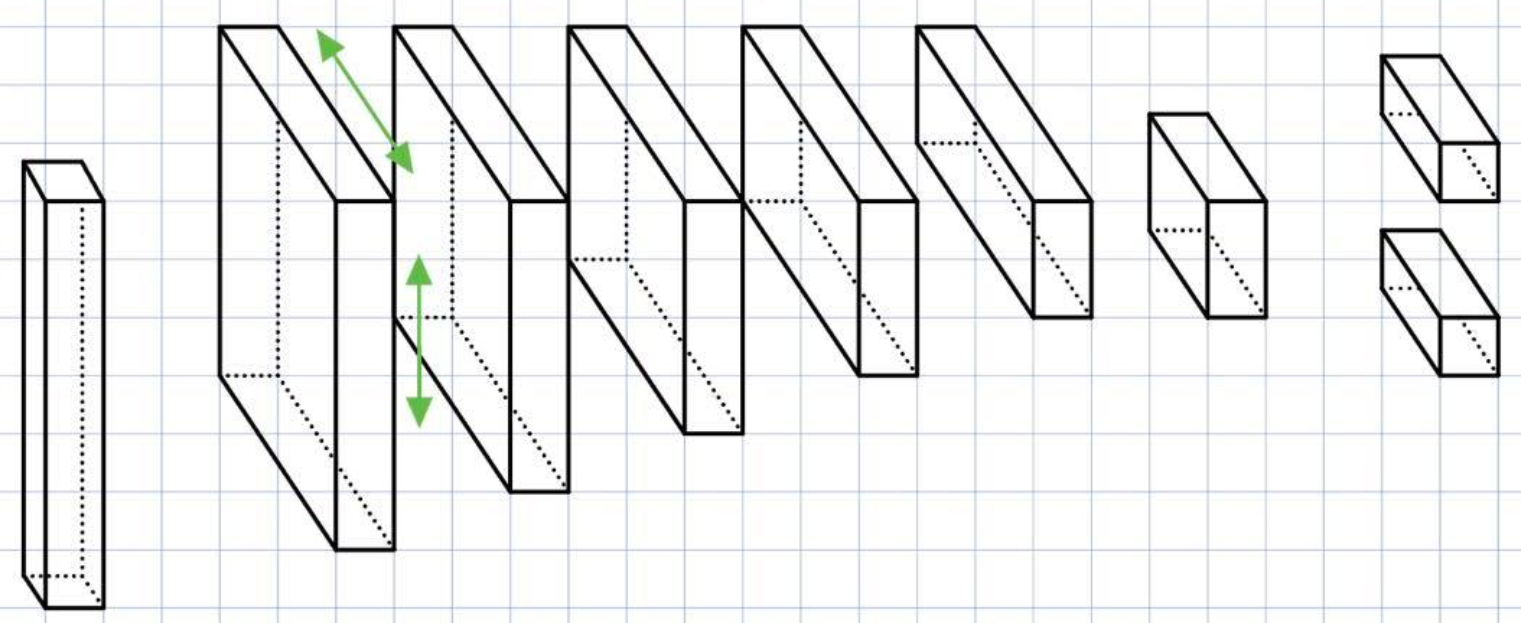
\includegraphics[width=0.7\linewidth]{architecture}
			\caption{}
			\label{fig:architecture}
		\end{figure}
	
		Figure \ref{fig:architecture} displays how via contrastive predictive coding an input speech signal is transformed into two latent vectors. The two vectors combined describe a Gaussian distribution for each feature of the latent representation. One vector corresponds to the means and the other to the standard deviations of the latent distributions. We variational autoencoders assume independent latent features, such that the covariance matrix is non negative on the diagonal and zero off the diagonal. This allows the covariance matrix to be described using a single vector. We again, make use of this (plausible incorrect?) assumption of having independent latent features.




		% Training on longer patches, classification on padded sub-patches.
		During inference, (in this context obtaining the latent representations for our input signals), depending on the length of the input signal, the length of the output latent representation will differ.
		If we wish to look at how separable latent representations are for syllables, the length can be variable. Some input sounds could be 6,600 samples, while others 8,800 samples. We therefore pad the syllables with zeroes in front and end of the signal, to obtain fixed length of equal to that of the longest syllable; 8,800 samples.
		
		Training happens on longer data samples, and every \textbf{X} epochs t-SNE visualisations are made to observe evolutional of dis-entanglement.
		

\section{Results}

	% Enkele loss curces etc
	\subsection{Results CPC}
	
	\begin{figure}[h] % distr beta = 0, module 1
		\centering
				\begin{subfigure}[b]{0.45\textwidth}
			\centering
			% This file was created with tikzplotlib v0.10.1.
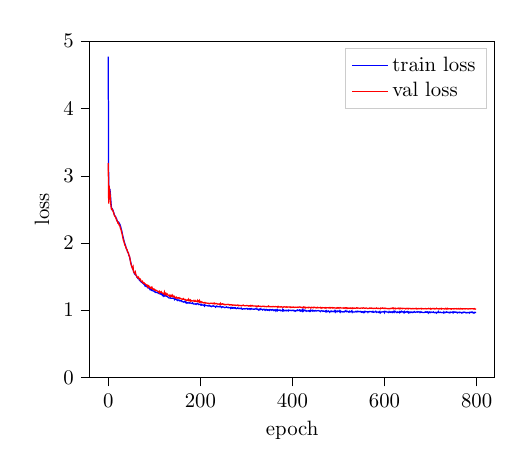
\begin{tikzpicture}[scale=0.75]

\definecolor{darkgray176}{RGB}{176,176,176}
\definecolor{lightgray204}{RGB}{204,204,204}

\begin{axis}[
legend cell align={left},
legend style={fill opacity=0.8, draw opacity=1, text opacity=1, draw=lightgray204},
tick align=outside,
tick pos=left,
x grid style={darkgray176},
xlabel={epoch},
xmin=-39.95, xmax=838.95,
xtick style={color=black},
y grid style={darkgray176},
ylabel={loss},
%ymin=0.766462631026904, ymax=4.9639792372783,
ymin=0, ymax=5,
ytick style={color=black}
]
\addplot [semithick, blue]
table {%
0 4.77318302790324
1 2.82349546750387
2 2.64447561899821
3 2.77237407366435
4 2.78129434585571
5 2.7005729675293
6 2.60248470306396
7 2.52906648317973
8 2.50064452489217
9 2.50624068578084
10 2.49251842498779
11 2.47220285733541
12 2.45464158058167
13 2.42697429656982
14 2.40570044517517
15 2.39877390861511
16 2.39136123657227
17 2.3739488919576
18 2.36341786384583
19 2.34293206532796
20 2.32241646448771
21 2.31134144465129
22 2.31324466069539
23 2.30598990122477
24 2.29167668024699
25 2.2839986483256
26 2.26445070902506
27 2.24438762664795
28 2.21447086334229
29 2.1932524840037
30 2.1603479385376
31 2.12762029965719
32 2.09522064526876
33 2.07273952166239
34 2.04036005338033
35 2.01156930128733
36 1.99235769112905
37 1.97092076142629
38 1.95159558455149
39 1.92247450351715
40 1.91070024172465
41 1.89166037241618
42 1.87214843432109
43 1.857958873113
44 1.84082369009654
45 1.81239640712738
46 1.80266439914703
47 1.77085427443186
48 1.74382936954498
49 1.7113550901413
50 1.6837116877238
51 1.65848024686178
52 1.63519390424093
53 1.63980011145274
54 1.60514783859253
55 1.58419768015544
56 1.55903752644857
57 1.54388833045959
58 1.54807595411936
59 1.52696160475413
60 1.52489956219991
61 1.51568480332692
62 1.49394702911377
63 1.48710914452871
64 1.47856386502584
65 1.47011439005534
66 1.46716018517812
67 1.46394801139832
68 1.44238332907359
69 1.44375669956207
70 1.4335701862971
71 1.42323748270671
72 1.41885268688202
73 1.41401668389638
74 1.41122730573018
75 1.401264945666
76 1.39735496044159
77 1.39205233256022
78 1.3812464872996
79 1.37892401218414
80 1.36239043871562
81 1.36717069149017
82 1.35402238368988
83 1.35631310939789
84 1.3511666059494
85 1.34234388669332
86 1.3422513405482
87 1.33544274171193
88 1.3297127087911
89 1.33126401901245
90 1.3194743792216
91 1.30526391665141
92 1.30877868334452
93 1.30192887783051
94 1.29791943232218
95 1.30909351507823
96 1.29058531920115
97 1.29049571355184
98 1.28703983624776
99 1.28414579232534
100 1.28646012147268
101 1.27306302388509
102 1.27423894405365
103 1.264550725619
104 1.26555025577545
105 1.26603921254476
106 1.26473859945933
107 1.26149725914001
108 1.26423680782318
109 1.25020829836528
110 1.25313222408295
111 1.24979257583618
112 1.24503072102865
113 1.24018307526906
114 1.24317272504171
115 1.25724335511525
116 1.23603761196136
117 1.22750008106232
118 1.21925671895345
119 1.23145218690236
120 1.2124350865682
121 1.22306029001872
122 1.21448290348053
123 1.23192656040192
124 1.21968003114065
125 1.23131843407949
126 1.21075137456258
127 1.2064360777537
128 1.20748368899028
129 1.19925999641418
130 1.19519253571828
131 1.19036146004995
132 1.18161722024282
133 1.18319284915924
134 1.18234586715698
135 1.18546561400096
136 1.17787369092305
137 1.17935752868652
138 1.1804358959198
139 1.18006678422292
140 1.17842284838359
141 1.18032077948252
142 1.18326663970947
143 1.17977511882782
144 1.15732022126516
145 1.16289103031158
146 1.16928092638652
147 1.16585028171539
148 1.16038397947947
149 1.15419975916545
150 1.14527599016825
151 1.14262692133586
152 1.15447402000427
153 1.15435508886973
154 1.15094105402629
155 1.14165997505188
156 1.13765569527944
157 1.13995762666066
158 1.1406538883845
159 1.14025433858236
160 1.13039982318878
161 1.13338955243429
162 1.1289381980896
163 1.12131083011627
164 1.12349196275075
165 1.12611663341522
166 1.13345650831858
167 1.12232704957326
168 1.12751011053721
169 1.11109721660614
170 1.11611882845561
171 1.10614200433095
172 1.11232415835063
173 1.10961806774139
174 1.10921041170756
175 1.11223423480988
176 1.10653785864512
177 1.11308101812998
178 1.10848693052928
179 1.10770217577616
180 1.10281292597453
181 1.10221457481384
182 1.10035920143127
183 1.1115779876709
184 1.1045831044515
185 1.09462873140971
186 1.094606757164
187 1.09277880191803
188 1.09322933355967
189 1.09679925441742
190 1.08820176124573
191 1.08663765589396
192 1.09593113263448
193 1.10153563817342
194 1.09681351979574
195 1.09624433517456
196 1.08609584967295
197 1.08926737308502
198 1.08899700641632
199 1.08961232503255
200 1.08061075210571
201 1.08885606129964
202 1.09035646915436
203 1.07667358716329
204 1.08042101065318
205 1.07912158966064
206 1.07634274164836
207 1.07277381420135
208 1.0785471200943
209 1.06415164470673
210 1.0794130563736
211 1.07321592171987
212 1.06975829601288
213 1.06926842530568
214 1.07006641228994
215 1.06723654270172
216 1.06544578075409
217 1.06225927670797
218 1.06297198931376
219 1.07384459177653
220 1.06515697638194
221 1.06526243686676
222 1.0608518520991
223 1.06276373068492
224 1.05410369237264
225 1.05742315451304
226 1.0597011645635
227 1.06411520640055
228 1.06796729564667
229 1.06041852633158
230 1.06095004081726
231 1.05889292558034
232 1.05696519215902
233 1.04580064614614
234 1.0516242980957
235 1.06281129519145
236 1.06305960814158
237 1.05549895763397
238 1.05199646949768
239 1.05362021923065
240 1.05359323819478
241 1.05656766891479
242 1.05213252703349
243 1.06234037876129
244 1.05786236127218
245 1.05093983809153
246 1.04032131036123
247 1.04546431700389
248 1.05183180173238
249 1.05195717016856
250 1.04829680919647
251 1.04673532644908
252 1.04329903920492
253 1.03898719946543
254 1.03956147034963
255 1.04201662540436
256 1.04609823226929
257 1.05024178822835
258 1.04539628823598
259 1.04060065746307
260 1.03779359658559
261 1.04301071166992
262 1.03717815876007
263 1.03865083058675
264 1.03739094734192
265 1.03955753644307
266 1.02803464730581
267 1.03915723164876
268 1.03358995914459
269 1.04064186414083
270 1.03132526079814
271 1.03467845916748
272 1.03808120886485
273 1.02979187170664
274 1.03558989365896
275 1.03247443834941
276 1.03823328018188
277 1.02722001075745
278 1.0228374004364
279 1.02738813559214
280 1.03046441078186
281 1.03686873118083
282 1.02669966220856
283 1.02911615371704
284 1.02476946512858
285 1.02876893679301
286 1.02726980050405
287 1.0298015276591
288 1.02435207366943
289 1.03140811125437
290 1.02210676670074
291 1.01501977443695
292 1.01677540938059
293 1.02146065235138
294 1.02300560474396
295 1.02245398362478
296 1.01983034610748
297 1.02148914337158
298 1.02162424723307
299 1.02027732133865
300 1.02532470226288
301 1.025767882665
302 1.02523505687714
303 1.01607565085093
304 1.02189477284749
305 1.01794115702311
306 1.01985788345337
307 1.02350171407064
308 1.0137255191803
309 1.02074035008748
310 1.02141773700714
311 1.024866938591
312 1.01800984144211
313 1.02021837234497
314 1.01971501111984
315 1.01485828558604
316 1.01570183038712
317 1.01759858926137
318 1.01647897561391
319 1.01957764228185
320 1.0184770822525
321 1.02758785088857
322 1.01726380983988
323 1.01533321539561
324 1.01872233549754
325 1.01701664924622
326 1.00336035092672
327 1.00953718026479
328 1.01429533958435
329 1.00724504391352
330 1.02109789848328
331 1.01288839181264
332 1.01762211322784
333 1.0147590637207
334 1.01303652922312
335 1.00367915630341
336 1.01085519790649
337 1.01027083396912
338 1.01565170288086
339 1.00673230489095
340 1.01014991601308
341 0.999194403489431
342 1.0055939356486
343 1.01296003659566
344 1.00492527087529
345 1.00191901127497
346 1.00688960154851
347 1.00080978870392
348 1.00572536389033
349 1.00737343231837
350 0.999158402283986
351 1.01136179765066
352 1.01081645488739
353 1.00390926996867
354 1.00673174858093
355 1.00002576907476
356 1.0088059703509
357 1.01115338007609
358 1.00895631313324
359 0.995758175849915
360 0.998561143875122
361 1.00477683544159
362 0.997286081314087
363 1.00347085793813
364 0.990313867727915
365 1.00827244917552
366 1.00308215618134
367 0.993881503740946
368 1.00817743937174
369 0.998443086942037
370 1.00041995445887
371 0.998472213745117
372 1.00179465611776
373 1.00496967633565
374 0.99479067325592
375 0.991618454456329
376 0.995748301347097
377 0.997022807598114
378 0.992162764072418
379 1.01201113065084
380 0.994642357031504
381 1.00269607702891
382 0.992556889851888
383 0.99697881937027
384 0.997688472270966
385 0.99444834391276
386 1.00074207782745
387 0.993134160836538
388 0.9981822570165
389 1.00015020370483
390 0.994283556938171
391 0.989677647749583
392 1.00291868050893
393 0.999600728352865
394 0.997915069262187
395 0.999336242675781
396 0.996019701162974
397 0.99842909971873
398 0.993980268637339
399 0.998267312844594
400 0.997798879941305
401 1.00089557965597
402 0.996208429336548
403 0.998635053634644
404 0.987486640612284
405 0.99400269985199
406 0.992410699526469
407 0.985347131888072
408 0.995540698369344
409 0.999054769674937
410 0.997415204842885
411 1.00424967209498
412 0.994718690713247
413 0.99588018655777
414 0.997307101885478
415 1.00417955716451
416 0.99402791261673
417 1.00086975097656
418 0.986425260702769
419 0.986976484457652
420 0.993578473726908
421 1.00586251417796
422 0.989299496014913
423 1.00880302985509
424 0.987371027469635
425 0.994316736857096
426 0.997924049695333
427 1.00333871444066
428 0.994100868701935
429 0.995581209659576
430 0.984843631585439
431 0.990061481793722
432 0.987317482630412
433 0.987607498963674
434 0.99085017045339
435 0.989208022753398
436 0.994175394376119
437 0.984116752942403
438 0.991821050643921
439 0.985806524753571
440 1.00215325752894
441 0.995361189047495
442 0.993731220563253
443 0.98835676908493
444 0.999169031778971
445 0.994167268276215
446 0.994577407836914
447 0.986076315244039
448 0.992286701997121
449 0.995156983534495
450 0.99592516819636
451 0.988463719685872
452 0.989400406678518
453 0.991093019644419
454 0.993026534716288
455 0.991647521654765
456 0.996180176734924
457 0.992725074291229
458 0.99130767583847
459 0.987074057261149
460 0.985625465710958
461 0.98018471399943
462 0.990522265434265
463 0.995668927828471
464 0.993494272232056
465 0.99093614021937
466 0.983717083930969
467 0.985197405020396
468 0.989650090535482
469 0.985493878523509
470 0.986208538214366
471 0.981104493141174
472 0.989290853341421
473 0.978047847747803
474 0.991539637247721
475 0.980186005433401
476 0.984004954497019
477 0.979789058367411
478 0.989546338717143
479 0.985851585865021
480 0.9814825852712
481 0.971488416194916
482 0.982728600502014
483 0.982302526632945
484 0.990212678909302
485 0.980808099110921
486 0.978102207183838
487 0.984086592992147
488 0.986159205436707
489 0.983742197354635
490 0.978950202465057
491 0.984819332758586
492 0.994552155335744
493 0.974896470705668
494 0.988852481047312
495 0.978783090909322
496 0.984478255112966
497 0.978518505891164
498 0.988398909568787
499 0.98401939868927
500 0.987609128157298
501 0.987914880116781
502 0.980099240938822
503 0.992740869522095
504 0.97374302148819
505 0.986462950706482
506 0.982351998488108
507 0.978004038333893
508 0.974581360816956
509 0.977119147777557
510 0.979325234889984
511 0.975952009359995
512 0.973198354244232
513 0.985048751036326
514 0.982684731483459
515 0.987491726875305
516 0.995139022668203
517 0.978458166122437
518 0.978292127450307
519 0.985782702763875
520 0.983109215895335
521 0.980572740236918
522 0.973398407300313
523 0.970669408639272
524 0.984611908594767
525 0.978074630101522
526 0.975667039553324
527 0.978140632311503
528 0.987409830093384
529 0.992791752020518
530 0.970087031523387
531 0.978887816270193
532 0.974406778812408
533 0.975158949693044
534 0.974492927392324
535 0.975346326828003
536 0.976473132769267
537 0.983329057693481
538 0.97741182645162
539 0.982467552026113
540 0.975909094015757
541 0.978306214014689
542 0.986021836598714
543 0.978562513987223
544 0.979986786842346
545 0.979821304480235
546 0.979385276635488
547 0.982568343480428
548 0.97709600130717
549 0.979777673880259
550 0.971911748250326
551 0.9778946240743
552 0.977550367514292
553 0.96910305817922
554 0.974399487177531
555 0.966692984104156
556 0.980726420879364
557 0.972916305065155
558 0.982898732026418
559 0.983507951100667
560 0.977215747038523
561 0.978801071643829
562 0.979653398195902
563 0.979268570741018
564 0.968430121739705
565 0.978812992572784
566 0.979154487450918
567 0.976821442445119
568 0.982877492904663
569 0.981142004330953
570 0.979298869768778
571 0.979425311088562
572 0.975968698660533
573 0.981699089209239
574 0.974335451920827
575 0.982049763202667
576 0.970686197280884
577 0.971425473690033
578 0.973110775152842
579 0.974015394846598
580 0.980320115884145
581 0.98606797059377
582 0.975744068622589
583 0.968281865119934
584 0.975185692310333
585 0.975420316060384
586 0.974225441614787
587 0.968505263328552
588 0.974172631899516
589 0.968145847320557
590 0.980003555615743
591 0.962411264578501
592 0.970946709314982
593 0.972045282522837
594 0.97475129365921
595 0.976983984311422
596 0.97574790318807
597 0.975930432478587
598 0.97842796643575
599 0.981857101122538
600 0.964972138404846
601 0.982097387313843
602 0.979564428329468
603 0.982954422632853
604 0.97627466917038
605 0.97483374675115
606 0.972867091496786
607 0.972493489583333
608 0.970237950483958
609 0.966216067473094
610 0.981039702892303
611 0.972168644269307
612 0.973717331886292
613 0.969411253929138
614 0.977225244045258
615 0.974056998888651
616 0.968641539414724
617 0.975370824337006
618 0.966817378997803
619 0.973647773265839
620 0.982434431711833
621 0.970868647098541
622 0.984674791495005
623 0.977852205435435
624 0.981652716795603
625 0.972910463809967
626 0.971175452073415
627 0.965049862861633
628 0.974063555399577
629 0.970737874507904
630 0.971841812133789
631 0.970213154951731
632 0.977654258410136
633 0.96525518099467
634 0.977625211079915
635 0.97088227669398
636 0.976237952709198
637 0.984388550122579
638 0.974150458971659
639 0.97512682278951
640 0.9796076019605
641 0.972622116406759
642 0.964066843191783
643 0.979873716831207
644 0.967878301938375
645 0.974310119946798
646 0.971816758314768
647 0.976560473442078
648 0.978116830190023
649 0.971834460894267
650 0.980676253636678
651 0.975660602251689
652 0.963904996713003
653 0.974164287249247
654 0.964964171250661
655 0.972234904766083
656 0.973644892374674
657 0.967475871245066
658 0.973986268043518
659 0.973434527715047
660 0.966661353905996
661 0.971389651298523
662 0.967136561870575
663 0.971375564734141
664 0.978911022345225
665 0.980407973130544
666 0.971928656101227
667 0.968379179636637
668 0.970372637112935
669 0.973975539207458
670 0.976503630479177
671 0.979294200738271
672 0.971852918465932
673 0.972858806451162
674 0.977224230766296
675 0.97346309820811
676 0.975266297658285
677 0.964694043000539
678 0.969182471434275
679 0.978262762228648
680 0.972481111685435
681 0.969014624754588
682 0.969340642293294
683 0.966596186161041
684 0.967128376166026
685 0.967366973559062
686 0.965617020924886
687 0.970353662967682
688 0.971198598543803
689 0.976458827654521
690 0.969665070374807
691 0.97083055973053
692 0.975877225399017
693 0.970661242802938
694 0.975173453489939
695 0.959020415941874
696 0.968898018201192
697 0.972191830476125
698 0.975710451602936
699 0.964645405610402
700 0.970426519711812
701 0.974340856075287
702 0.971760114034017
703 0.967306574185689
704 0.969853738943736
705 0.971393565336863
706 0.975995083649953
707 0.96746027469635
708 0.968015650908152
709 0.963340123494466
710 0.964515864849091
711 0.969387451807658
712 0.968196630477905
713 0.95882644255956
714 0.970125297705332
715 0.969966729482015
716 0.967481036980947
717 0.980506996313731
718 0.966641287008921
719 0.965403020381927
720 0.968972762425741
721 0.972157677014669
722 0.968838353951772
723 0.964846650759379
724 0.966631809870402
725 0.967106918493907
726 0.966839094956716
727 0.965678950150808
728 0.961091697216034
729 0.976930280526479
730 0.969932933648427
731 0.962427874406179
732 0.968680282433828
733 0.969242691993713
734 0.973547379175822
735 0.977297325929006
736 0.968383073806763
737 0.971770683924357
738 0.971964617570241
739 0.966383775075277
740 0.963698844114939
741 0.961479465166728
742 0.971028288205465
743 0.964948097864787
744 0.971877674261729
745 0.96917865673701
746 0.969457050164541
747 0.969050923983256
748 0.974046965440114
749 0.960827628771464
750 0.97017506758372
751 0.978243748346964
752 0.970496714115143
753 0.969222009181976
754 0.974244316418966
755 0.971182783444723
756 0.972101787726084
757 0.966466089089712
758 0.960623403390249
759 0.969286223252614
760 0.965993026892344
761 0.965990404287974
762 0.972123205661774
763 0.964775522549947
764 0.970292607943217
765 0.966280241807302
766 0.968728721141815
767 0.962765177090963
768 0.957258840401967
769 0.963924407958984
770 0.96856427192688
771 0.971259216467539
772 0.965835789839427
773 0.973560750484467
774 0.970288455486298
775 0.970431566238403
776 0.966421107451121
777 0.961062252521515
778 0.965643505255381
779 0.962040483951569
780 0.965963363647461
781 0.964816013971964
782 0.96634715795517
783 0.964792927106222
784 0.957991659641266
785 0.969284395376841
786 0.972879389921824
787 0.966335753599803
788 0.965797742207845
789 0.972991387049357
790 0.975750923156738
791 0.965976854165395
792 0.969976902008057
793 0.964464008808136
794 0.957401712735494
795 0.95826256275177
796 0.970207432905833
797 0.968756298224131
798 0.965933779875437
799 0.966743965943654
};
\addlegendentry{train loss}
\addplot [semithick, red]
table {%
0 3.18817353248596
1 2.58615636825562
2 2.74251127243042
3 2.79088640213013
4 2.7313449382782
5 2.63192105293274
6 2.5462920665741
7 2.50334215164185
8 2.50713658332825
9 2.5010027885437
10 2.4782075881958
11 2.46338891983032
12 2.44067049026489
13 2.41785597801208
14 2.40613579750061
15 2.39184784889221
16 2.38242840766907
17 2.36530947685242
18 2.34402179718018
19 2.3277907371521
20 2.32069325447083
21 2.2976393699646
22 2.30218243598938
23 2.27970910072327
24 2.26445984840393
25 2.26277756690979
26 2.23212623596191
27 2.21221208572388
28 2.19356822967529
29 2.16065192222595
30 2.13969898223877
31 2.10676074028015
32 2.06871342658997
33 2.0383186340332
34 2.02660250663757
35 1.99751889705658
36 1.97040677070618
37 1.96310830116272
38 1.93828547000885
39 1.92580032348633
40 1.90227723121643
41 1.90006577968597
42 1.86582314968109
43 1.86290955543518
44 1.85060250759125
45 1.81429898738861
46 1.80558395385742
47 1.77832221984863
48 1.73388040065765
49 1.69674074649811
50 1.6741281747818
51 1.64896082878113
52 1.6374853849411
53 1.61972224712372
54 1.64082527160645
55 1.57291150093079
56 1.56644010543823
57 1.55988442897797
58 1.54774045944214
59 1.56632912158966
60 1.52742314338684
61 1.52018141746521
62 1.50289583206177
63 1.49477660655975
64 1.48228120803833
65 1.47832882404327
66 1.48987686634064
67 1.46968853473663
68 1.46834421157837
69 1.45391237735748
70 1.45970177650452
71 1.43787217140198
72 1.4316680431366
73 1.42498290538788
74 1.43123114109039
75 1.41618978977203
76 1.40261292457581
77 1.41165089607239
78 1.40649938583374
79 1.39647495746613
80 1.39379227161407
81 1.38716912269592
82 1.38357770442963
83 1.37367868423462
84 1.36613607406616
85 1.37090933322906
86 1.34751093387604
87 1.36771559715271
88 1.36405205726624
89 1.35039258003235
90 1.33873820304871
91 1.34015738964081
92 1.32924592494965
93 1.33906960487366
94 1.33025097846985
95 1.34178674221039
96 1.32359766960144
97 1.31170737743378
98 1.31263315677643
99 1.31707072257996
100 1.31450033187866
101 1.30316090583801
102 1.29488742351532
103 1.29976737499237
104 1.29593420028687
105 1.29337871074677
106 1.28589153289795
107 1.28491842746735
108 1.28128349781036
109 1.27904903888702
110 1.26756727695465
111 1.27880072593689
112 1.26124632358551
113 1.27041327953339
114 1.26899349689484
115 1.27677774429321
116 1.26418721675873
117 1.25915229320526
118 1.2510871887207
119 1.25005304813385
120 1.24921047687531
121 1.24150705337524
122 1.26874947547913
123 1.23959147930145
124 1.2446014881134
125 1.25270962715149
126 1.22552645206451
127 1.23356246948242
128 1.24300289154053
129 1.23398637771606
130 1.22319447994232
131 1.22148418426514
132 1.2159640789032
133 1.20994472503662
134 1.2236133813858
135 1.20778274536133
136 1.21412944793701
137 1.22134864330292
138 1.20472526550293
139 1.20184016227722
140 1.22093331813812
141 1.20479321479797
142 1.20874178409576
143 1.21009969711304
144 1.19152724742889
145 1.19239807128906
146 1.19223940372467
147 1.18214869499207
148 1.19305419921875
149 1.18188178539276
150 1.17984616756439
151 1.18431735038757
152 1.18533945083618
153 1.18078136444092
154 1.18610954284668
155 1.17508554458618
156 1.17830419540405
157 1.17863392829895
158 1.16828060150146
159 1.16636800765991
160 1.16763269901276
161 1.16103255748749
162 1.16547238826752
163 1.1731618642807
164 1.16259241104126
165 1.16332626342773
166 1.16162776947021
167 1.16119503974915
168 1.15910089015961
169 1.14385008811951
170 1.14813721179962
171 1.15210461616516
172 1.14721143245697
173 1.14651584625244
174 1.16259479522705
175 1.14222919940948
176 1.14284646511078
177 1.15252459049225
178 1.1425449848175
179 1.15204000473022
180 1.13583159446716
181 1.14176797866821
182 1.14071226119995
183 1.13991725444794
184 1.13830423355103
185 1.13695311546326
186 1.14511156082153
187 1.13077795505524
188 1.13159108161926
189 1.1427971124649
190 1.13470482826233
191 1.13568568229675
192 1.13321614265442
193 1.12954139709473
194 1.14626085758209
195 1.13081252574921
196 1.13734316825867
197 1.12675297260284
198 1.14312660694122
199 1.12226891517639
200 1.12788724899292
201 1.11685061454773
202 1.12192595005035
203 1.12653577327728
204 1.11951243877411
205 1.11376738548279
206 1.11477315425873
207 1.11319375038147
208 1.10788369178772
209 1.11205041408539
210 1.11664378643036
211 1.10666418075562
212 1.10582673549652
213 1.10840511322021
214 1.10745799541473
215 1.10595858097076
216 1.1029189825058
217 1.10543930530548
218 1.10435271263123
219 1.09907412528992
220 1.09950697422028
221 1.10245823860168
222 1.1040370464325
223 1.10559523105621
224 1.10411846637726
225 1.10543966293335
226 1.10275328159332
227 1.09848380088806
228 1.10498344898224
229 1.09960436820984
230 1.0960818529129
231 1.10512781143188
232 1.09729194641113
233 1.09779965877533
234 1.09864068031311
235 1.10109841823578
236 1.0987982749939
237 1.09342527389526
238 1.0907084941864
239 1.09164941310883
240 1.09134078025818
241 1.09108769893646
242 1.09492087364197
243 1.08814835548401
244 1.10264790058136
245 1.08941674232483
246 1.08724975585938
247 1.0888934135437
248 1.09740495681763
249 1.09557163715363
250 1.09042513370514
251 1.08595812320709
252 1.08866441249847
253 1.0818235874176
254 1.08486139774323
255 1.08188700675964
256 1.08569979667664
257 1.08552157878876
258 1.08528172969818
259 1.08536553382874
260 1.08884310722351
261 1.08605968952179
262 1.08229613304138
263 1.08338952064514
264 1.0764240026474
265 1.08104121685028
266 1.08026278018951
267 1.08129286766052
268 1.07891654968262
269 1.08170652389526
270 1.07380259037018
271 1.0747401714325
272 1.07757771015167
273 1.07855081558228
274 1.07776272296906
275 1.07274675369263
276 1.07482838630676
277 1.07674586772919
278 1.07487607002258
279 1.0726306438446
280 1.07578933238983
281 1.07832205295563
282 1.07683062553406
283 1.06675410270691
284 1.06923043727875
285 1.07307767868042
286 1.07041251659393
287 1.07060217857361
288 1.06877183914185
289 1.0655642747879
290 1.07115054130554
291 1.07038772106171
292 1.06940877437592
293 1.07706022262573
294 1.06916308403015
295 1.06930601596832
296 1.06778049468994
297 1.06747210025787
298 1.06747651100159
299 1.06685948371887
300 1.07050335407257
301 1.06966161727905
302 1.07144105434418
303 1.06637942790985
304 1.06542873382568
305 1.06150841712952
306 1.06574440002441
307 1.06549143791199
308 1.06272923946381
309 1.07031428813934
310 1.06463921070099
311 1.06852328777313
312 1.06375646591187
313 1.07051062583923
314 1.06602096557617
315 1.06212031841278
316 1.06255269050598
317 1.062420129776
318 1.06329047679901
319 1.06271398067474
320 1.06134569644928
321 1.06266713142395
322 1.05444014072418
323 1.06091582775116
324 1.05444920063019
325 1.0612565279007
326 1.06586289405823
327 1.05943393707275
328 1.05880832672119
329 1.05840587615967
330 1.05802845954895
331 1.05879926681519
332 1.05279946327209
333 1.05591189861298
334 1.05803883075714
335 1.06002879142761
336 1.05906987190247
337 1.06072008609772
338 1.05617547035217
339 1.05831778049469
340 1.05386900901794
341 1.05645155906677
342 1.05672085285187
343 1.05287575721741
344 1.05353081226349
345 1.05632042884827
346 1.05492496490479
347 1.05241751670837
348 1.06250953674316
349 1.05418789386749
350 1.05266690254211
351 1.05588579177856
352 1.05306315422058
353 1.05395221710205
354 1.05418491363525
355 1.05209827423096
356 1.05396950244904
357 1.05374026298523
358 1.05732131004333
359 1.05317175388336
360 1.05099940299988
361 1.052605509758
362 1.05295860767365
363 1.05585134029388
364 1.05304408073425
365 1.05133235454559
366 1.05355763435364
367 1.0528302192688
368 1.04668366909027
369 1.05785036087036
370 1.0499769449234
371 1.04830551147461
372 1.04967510700226
373 1.051837682724
374 1.04730629920959
375 1.05042433738708
376 1.05309498310089
377 1.04838418960571
378 1.04838752746582
379 1.04576599597931
380 1.04465568065643
381 1.05030882358551
382 1.05217504501343
383 1.05032789707184
384 1.0469411611557
385 1.04653704166412
386 1.04994106292725
387 1.04548299312592
388 1.05006492137909
389 1.04593634605408
390 1.04848325252533
391 1.04994297027588
392 1.04875564575195
393 1.04637825489044
394 1.0476496219635
395 1.05082857608795
396 1.04216694831848
397 1.04490292072296
398 1.0424497127533
399 1.04764199256897
400 1.04313778877258
401 1.04312908649445
402 1.04843354225159
403 1.04361367225647
404 1.04362142086029
405 1.04081654548645
406 1.04605305194855
407 1.04406487941742
408 1.04504084587097
409 1.04463911056519
410 1.04331755638123
411 1.04595601558685
412 1.04171943664551
413 1.04392409324646
414 1.04743087291718
415 1.04995620250702
416 1.0457319021225
417 1.04618346691132
418 1.04838621616364
419 1.04421257972717
420 1.04079914093018
421 1.04207897186279
422 1.04345381259918
423 1.04082989692688
424 1.04757285118103
425 1.03757441043854
426 1.04125261306763
427 1.04730808734894
428 1.03574156761169
429 1.04203033447266
430 1.04257798194885
431 1.03967118263245
432 1.04283916950226
433 1.04067647457123
434 1.03649616241455
435 1.04365181922913
436 1.04304707050323
437 1.043088555336
438 1.03918528556824
439 1.0390008687973
440 1.03115689754486
441 1.04504287242889
442 1.04444050788879
443 1.04047012329102
444 1.04124402999878
445 1.03685760498047
446 1.04434394836426
447 1.04164755344391
448 1.04411637783051
449 1.04032349586487
450 1.03835427761078
451 1.03954088687897
452 1.03531289100647
453 1.03903722763062
454 1.0438015460968
455 1.03626978397369
456 1.03922188282013
457 1.03647744655609
458 1.03867149353027
459 1.03926765918732
460 1.03984141349792
461 1.04329442977905
462 1.03174066543579
463 1.03697991371155
464 1.03295397758484
465 1.04059839248657
466 1.03844010829926
467 1.03787434101105
468 1.03890883922577
469 1.0383335351944
470 1.03359937667847
471 1.03966426849365
472 1.03320562839508
473 1.03832304477692
474 1.03421545028687
475 1.03700232505798
476 1.03788816928864
477 1.03659784793854
478 1.03868234157562
479 1.03434550762177
480 1.03972434997559
481 1.04124569892883
482 1.03200817108154
483 1.03914296627045
484 1.03738164901733
485 1.03571045398712
486 1.04052066802979
487 1.03291463851929
488 1.03656446933746
489 1.03363835811615
490 1.03781175613403
491 1.03686332702637
492 1.0341329574585
493 1.03303813934326
494 1.03433001041412
495 1.02951693534851
496 1.03330886363983
497 1.04008531570435
498 1.03835296630859
499 1.03073883056641
500 1.03737163543701
501 1.03399968147278
502 1.03241610527039
503 1.03955686092377
504 1.03928279876709
505 1.03347539901733
506 1.03373241424561
507 1.03284108638763
508 1.03345477581024
509 1.03263068199158
510 1.03352010250092
511 1.03111529350281
512 1.03822708129883
513 1.03154444694519
514 1.03396677970886
515 1.03593480587006
516 1.0315455198288
517 1.03729605674744
518 1.03671216964722
519 1.02705204486847
520 1.03199207782745
521 1.03371584415436
522 1.0300726890564
523 1.03175151348114
524 1.03056001663208
525 1.03375065326691
526 1.02874529361725
527 1.03429567813873
528 1.02849721908569
529 1.03076982498169
530 1.02683353424072
531 1.03497588634491
532 1.02798366546631
533 1.02953803539276
534 1.03371739387512
535 1.03083658218384
536 1.03160524368286
537 1.02973556518555
538 1.02891397476196
539 1.03685534000397
540 1.03411483764648
541 1.03175532817841
542 1.03546440601349
543 1.03383994102478
544 1.03125989437103
545 1.03078508377075
546 1.02997958660126
547 1.02822768688202
548 1.03038704395294
549 1.03290617465973
550 1.03188824653625
551 1.0329749584198
552 1.02982842922211
553 1.03056967258453
554 1.03632867336273
555 1.03228986263275
556 1.03179323673248
557 1.03044724464417
558 1.02844333648682
559 1.03031826019287
560 1.03424024581909
561 1.03310441970825
562 1.02926874160767
563 1.02699446678162
564 1.02614676952362
565 1.02710926532745
566 1.02898871898651
567 1.03244304656982
568 1.03228354454041
569 1.02878844738007
570 1.02915954589844
571 1.0350102186203
572 1.03163158893585
573 1.02770376205444
574 1.03117215633392
575 1.03000366687775
576 1.02601754665375
577 1.02705347537994
578 1.02964627742767
579 1.02823722362518
580 1.02607703208923
581 1.03059113025665
582 1.03125250339508
583 1.03506529331207
584 1.02861249446869
585 1.02637541294098
586 1.02725493907928
587 1.03032255172729
588 1.02630734443665
589 1.02772176265717
590 1.0279837846756
591 1.02313959598541
592 1.03342425823212
593 1.03045105934143
594 1.02892541885376
595 1.03030836582184
596 1.03454172611237
597 1.02914214134216
598 1.02949190139771
599 1.02512431144714
600 1.030428647995
601 1.03349697589874
602 1.02759337425232
603 1.02613198757172
604 1.02778577804565
605 1.02471077442169
606 1.02463293075562
607 1.02327930927277
608 1.02487206459045
609 1.02407419681549
610 1.02388262748718
611 1.02203214168549
612 1.02820110321045
613 1.02426445484161
614 1.02806949615479
615 1.02674412727356
616 1.02687990665436
617 1.03368365764618
618 1.02862238883972
619 1.02308070659637
620 1.03165054321289
621 1.02411735057831
622 1.02649748325348
623 1.03154468536377
624 1.0218288898468
625 1.02673804759979
626 1.02634310722351
627 1.02625977993011
628 1.02904343605042
629 1.02690923213959
630 1.02775824069977
631 1.03132021427155
632 1.02165901660919
633 1.02735018730164
634 1.02308201789856
635 1.03021240234375
636 1.02497911453247
637 1.02475476264954
638 1.02939462661743
639 1.02289724349976
640 1.02578318119049
641 1.0271338224411
642 1.02918434143066
643 1.02747893333435
644 1.02484035491943
645 1.0239040851593
646 1.02015101909637
647 1.02856576442719
648 1.02623677253723
649 1.02321243286133
650 1.02765429019928
651 1.02558732032776
652 1.02053046226501
653 1.02877521514893
654 1.02652454376221
655 1.02689182758331
656 1.02373361587524
657 1.02539956569672
658 1.02148044109344
659 1.02083396911621
660 1.02613592147827
661 1.02356052398682
662 1.02518320083618
663 1.02294778823853
664 1.02465391159058
665 1.02411198616028
666 1.02185344696045
667 1.02613627910614
668 1.02782297134399
669 1.02251482009888
670 1.02709054946899
671 1.01992797851562
672 1.02192747592926
673 1.02257752418518
674 1.02630639076233
675 1.0236918926239
676 1.0232275724411
677 1.02443587779999
678 1.02556872367859
679 1.02481842041016
680 1.01959657669067
681 1.02728867530823
682 1.02318358421326
683 1.02260959148407
684 1.02073490619659
685 1.0222419500351
686 1.02348506450653
687 1.02294385433197
688 1.02274489402771
689 1.02517545223236
690 1.0229572057724
691 1.02028334140778
692 1.02089416980743
693 1.0234432220459
694 1.0224027633667
695 1.02187860012054
696 1.02816569805145
697 1.02411270141602
698 1.02346074581146
699 1.02114701271057
700 1.02665829658508
701 1.01741981506348
702 1.02360868453979
703 1.02451252937317
704 1.02340698242188
705 1.02595221996307
706 1.02409183979034
707 1.0254784822464
708 1.02131116390228
709 1.02524065971375
710 1.02026677131653
711 1.02178692817688
712 1.02484285831451
713 1.02989745140076
714 1.02121579647064
715 1.02192795276642
716 1.02341246604919
717 1.01939678192139
718 1.02272820472717
719 1.02028095722198
720 1.02568280696869
721 1.02163469791412
722 1.02380919456482
723 1.0190761089325
724 1.02724599838257
725 1.02147352695465
726 1.02337980270386
727 1.0211797952652
728 1.02187597751617
729 1.02266454696655
730 1.01995265483856
731 1.02054357528687
732 1.02268171310425
733 1.02830708026886
734 1.01817297935486
735 1.02373743057251
736 1.02098023891449
737 1.02840805053711
738 1.01962029933929
739 1.0233211517334
740 1.0228830575943
741 1.02191722393036
742 1.02103579044342
743 1.01987838745117
744 1.02179825305939
745 1.01683402061462
746 1.02352964878082
747 1.02248525619507
748 1.02375149726868
749 1.02185726165771
750 1.01993501186371
751 1.02468812465668
752 1.02010941505432
753 1.02226650714874
754 1.0208420753479
755 1.02146577835083
756 1.02467608451843
757 1.01844668388367
758 1.01954329013824
759 1.02197337150574
760 1.02341628074646
761 1.02614772319794
762 1.01760160923004
763 1.01886224746704
764 1.02027487754822
765 1.02556669712067
766 1.0194308757782
767 1.02156734466553
768 1.02210366725922
769 1.01816654205322
770 1.02362620830536
771 1.02210438251495
772 1.02369463443756
773 1.01991355419159
774 1.02203047275543
775 1.02229356765747
776 1.01991820335388
777 1.0222110748291
778 1.02173125743866
779 1.02091944217682
780 1.02153503894806
781 1.01861155033112
782 1.02164673805237
783 1.02019667625427
784 1.02083718776703
785 1.02331304550171
786 1.02042925357819
787 1.02071261405945
788 1.02276313304901
789 1.02242302894592
790 1.02295899391174
791 1.02299475669861
792 1.02282512187958
793 1.02326095104218
794 1.01872825622559
795 1.02407217025757
796 1.01759076118469
797 1.01637649536133
798 1.01789379119873
799 1.01713418960571
};
\addlegendentry{val loss}
\end{axis}

\end{tikzpicture}

			\caption{Module 1: $\beta=0.0035$}
		\end{subfigure}
		\hfill
		\begin{subfigure}[b]{0.45\textwidth}
			\centering
			% This file was created with tikzplotlib v0.10.1.
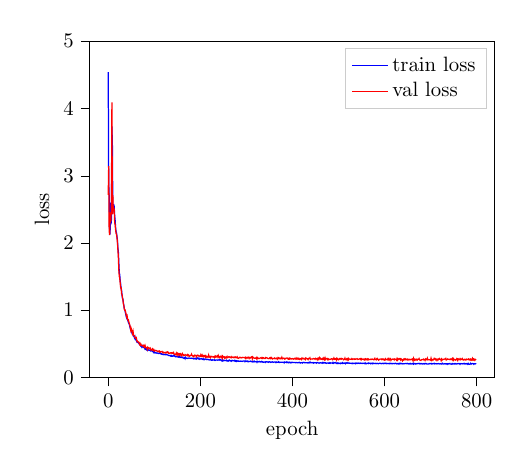
\begin{tikzpicture}[scale=0.75]

\definecolor{darkgray176}{RGB}{176,176,176}
\definecolor{lightgray204}{RGB}{204,204,204}

\begin{axis}[
legend cell align={left},
legend style={fill opacity=0.8, draw opacity=1, text opacity=1, draw=lightgray204},
tick align=outside,
tick pos=left,
x grid style={darkgray176},
xlabel={epoch},
xmin=-39.95, xmax=838.95,
xtick style={color=black},
y grid style={darkgray176},
ylabel={loss},
%ymin=-0.021006298561891, ymax=4.75973882526159,
ymin=0, ymax=5,
ytick style={color=black}
]
\addplot [semithick, blue]
table {%
0 4.54243222872416
1 2.91224869092306
2 2.70756467183431
3 2.20921150843302
4 2.12441794077555
5 2.59923768043518
6 2.27799201011658
7 2.3481650352478
8 3.7341996828715
9 3.47541880607605
10 2.49392302831014
11 2.57739162445068
12 2.50233284632365
13 2.52744952837626
14 2.40901843706767
15 2.33890557289124
16 2.23251644770304
17 2.170379002889
18 2.15254338582357
19 2.10055685043335
20 2.04287695884705
21 1.92793639500936
22 1.87178158760071
23 1.71000194549561
24 1.56501265366872
25 1.52897401650747
26 1.4415009021759
27 1.39354634284973
28 1.32204147179921
29 1.29988586902618
30 1.22322515646617
31 1.17662286758423
32 1.16533064842224
33 1.10909024874369
34 1.06669811407725
35 1.02210748195648
36 1.00717761119207
37 0.972453912099203
38 0.943314731121063
39 0.907348016897837
40 0.886219044526418
41 0.868048906326294
42 0.860821922620138
43 0.836703022321065
44 0.814626495043437
45 0.802799999713898
46 0.786758561929067
47 0.755470077196757
48 0.723514477411906
49 0.724357565244039
50 0.696030517419179
51 0.677563945452372
52 0.651315033435822
53 0.654884517192841
54 0.635948876539866
55 0.615236004193624
56 0.610344906648
57 0.591572244962057
58 0.6064639488856
59 0.560573995113373
60 0.558573583761851
61 0.558662454287211
62 0.528558989365896
63 0.530122796694438
64 0.520792643229167
65 0.517385641733805
66 0.510840396086375
67 0.502012133598328
68 0.4931700527668
69 0.485118051369985
70 0.477811147769292
71 0.463958313067754
72 0.461648672819138
73 0.450137943029404
74 0.468188325564067
75 0.452291667461395
76 0.452158600091934
77 0.447512894868851
78 0.444141695896784
79 0.433066775401433
80 0.421434670686722
81 0.431173692146937
82 0.424106448888779
83 0.414001941680908
84 0.423673033714294
85 0.407048185666402
86 0.423825492461522
87 0.409576753775279
88 0.405763864517212
89 0.407238811254501
90 0.404822478691737
91 0.399141887823741
92 0.394373993078868
93 0.397426605224609
94 0.396282802025477
95 0.397517383098602
96 0.385017096996307
97 0.384532352288564
98 0.381175915400187
99 0.371287435293198
100 0.388231406609217
101 0.368989835182826
102 0.372081061204274
103 0.365734418233236
104 0.367855419715246
105 0.364329049984614
106 0.361339569091797
107 0.365005761384964
108 0.365050892035166
109 0.355991582075755
110 0.355605016152064
111 0.359149356683095
112 0.36028328537941
113 0.357479939858119
114 0.353164861599604
115 0.348035633563995
116 0.354147960742315
117 0.347699880599976
118 0.342826664447784
119 0.345733275016149
120 0.340557942787806
121 0.343486070632935
122 0.3461674451828
123 0.339414179325104
124 0.339618057012558
125 0.337416837612788
126 0.340026577313741
127 0.339782565832138
128 0.340259204308192
129 0.334815929333369
130 0.332334687312444
131 0.326290786266327
132 0.326169590155284
133 0.327941646178563
134 0.324016173680623
135 0.319881856441498
136 0.327327171961466
137 0.31907785932223
138 0.326547851165136
139 0.315328309933345
140 0.315540234247843
141 0.3183873295784
142 0.328102320432663
143 0.321295936902364
144 0.323758572340012
145 0.313768704732259
146 0.314784566561381
147 0.307946940263112
148 0.310459911823273
149 0.310275634129842
150 0.307165374358495
151 0.308205644289653
152 0.301831632852554
153 0.303824216127396
154 0.318283875783284
155 0.302999248107274
156 0.298143694798152
157 0.305724153916041
158 0.303494026263555
159 0.299708555142085
160 0.295811196168264
161 0.302237162987391
162 0.295111189285914
163 0.289083590110143
164 0.287380745013555
165 0.291332691907883
166 0.296830375989278
167 0.280707766612371
168 0.299491425355275
169 0.290432850519816
170 0.287170926729838
171 0.284206291039785
172 0.286390900611877
173 0.283303459485372
174 0.287125587463379
175 0.290914356708527
176 0.288411358992259
177 0.287985652685165
178 0.284752080837886
179 0.286448250214259
180 0.285262723763784
181 0.287699888149897
182 0.283894240856171
183 0.286740610996882
184 0.286182234684626
185 0.281156380971273
186 0.275917182366053
187 0.279307623704274
188 0.280228535334269
189 0.286345918973287
190 0.277051866054535
191 0.272789130608241
192 0.285243928432465
193 0.283734450737635
194 0.289654433727264
195 0.279389003912608
196 0.276555716991425
197 0.286145945390065
198 0.272041231393814
199 0.275958657264709
200 0.276214212179184
201 0.27856300274531
202 0.274838874737422
203 0.279192417860031
204 0.273392289876938
205 0.270391533772151
206 0.276224335034688
207 0.268364111582438
208 0.274308353662491
209 0.265875329573949
210 0.271153410275777
211 0.274776488542557
212 0.275056262811025
213 0.269873708486557
214 0.266371200482051
215 0.267951836188634
216 0.270300428072612
217 0.26624650756518
218 0.264399240414302
219 0.266360352436701
220 0.261595696210861
221 0.261257479588191
222 0.264023651679357
223 0.266486714283625
224 0.25815490881602
225 0.260816136995951
226 0.257317026456197
227 0.264893730481466
228 0.260904371738434
229 0.260463337103526
230 0.258353849252065
231 0.263581256071726
232 0.253510112563769
233 0.255989263455073
234 0.260997196038564
235 0.259674280881882
236 0.261326014995575
237 0.258689562479655
238 0.256636296709379
239 0.261239091555278
240 0.261643826961517
241 0.264623632033666
242 0.259043057759603
243 0.262194414933523
244 0.26593475540479
245 0.257523556550344
246 0.250290478269259
247 0.256915380557378
248 0.248994534214338
249 0.262858202060064
250 0.256686429182688
251 0.248531758785248
252 0.253601888815562
253 0.254459192355474
254 0.252931416034698
255 0.254205122590065
256 0.251114666461945
257 0.258358548084895
258 0.247837275266647
259 0.249046494563421
260 0.241342614094416
261 0.245692784587542
262 0.25620877246062
263 0.260157893101374
264 0.252562870581945
265 0.245441834131877
266 0.248910074432691
267 0.252502232789993
268 0.243029475212097
269 0.249610046545664
270 0.254315555095673
271 0.251527920365334
272 0.247995505730311
273 0.248847345511119
274 0.245852659145991
275 0.255099674065908
276 0.242993553479513
277 0.247608905037244
278 0.239134833216667
279 0.247542272011439
280 0.242103531956673
281 0.243768205245336
282 0.248935808738073
283 0.242127686738968
284 0.239563246568044
285 0.242035915454229
286 0.243719687064489
287 0.242338175574938
288 0.244040538867315
289 0.240186333656311
290 0.240161960323652
291 0.242235312859217
292 0.239688495794932
293 0.245744859178861
294 0.244108830889066
295 0.244313433766365
296 0.245534181594849
297 0.234506825606028
298 0.23882024983565
299 0.24714769423008
300 0.243201792240143
301 0.238929897546768
302 0.239622036616007
303 0.24484221637249
304 0.23360113799572
305 0.237093587716421
306 0.23941304286321
307 0.2386208375295
308 0.237806235750516
309 0.243769417206446
310 0.244075124462446
311 0.235987658301989
312 0.235050782561302
313 0.232385983069738
314 0.241136138637861
315 0.233620911836624
316 0.232571353514989
317 0.243267079194387
318 0.234569524725278
319 0.233594809969266
320 0.235100150108337
321 0.234482884407043
322 0.23801230887572
323 0.226572304964066
324 0.239169334371885
325 0.233990480502447
326 0.234145368138949
327 0.232355485359828
328 0.239859059453011
329 0.236137901743253
330 0.234488313396772
331 0.230090195933978
332 0.23244567712148
333 0.239268417159716
334 0.231554041306178
335 0.23322506248951
336 0.227772668004036
337 0.226621170838674
338 0.231945728262266
339 0.231304536263148
340 0.232033242781957
341 0.224519843856494
342 0.23323896030585
343 0.234128768245379
344 0.231620043516159
345 0.233919719854991
346 0.230894943078359
347 0.230348706245422
348 0.225872337818146
349 0.233749836683273
350 0.234655434886614
351 0.231812303264936
352 0.225724577903748
353 0.230311165253321
354 0.226945489645004
355 0.23012646039327
356 0.229854310552279
357 0.233078653613726
358 0.225739479064941
359 0.228678613901138
360 0.228269656499227
361 0.230774099628131
362 0.231495648622513
363 0.231071472167969
364 0.223231603701909
365 0.230529884497325
366 0.223925828933716
367 0.226101179917653
368 0.226038222511609
369 0.228525976339976
370 0.234671254952749
371 0.224443172415098
372 0.227036654949188
373 0.224164853493373
374 0.227943723400434
375 0.227113862832387
376 0.227426980932554
377 0.225698331991831
378 0.225351835290591
379 0.227035587032636
380 0.227942203481992
381 0.226681083440781
382 0.217774202426275
383 0.230822076400121
384 0.227732678254445
385 0.226625472307205
386 0.225435813268026
387 0.230682462453842
388 0.223024924596151
389 0.229064241051674
390 0.22544585665067
391 0.219520290692647
392 0.226019660631816
393 0.222313975294431
394 0.228043178717295
395 0.225415706634521
396 0.21871417760849
397 0.223141660292943
398 0.220714822411537
399 0.227267488837242
400 0.222433045506477
401 0.224132786194483
402 0.222309629122416
403 0.222796315948168
404 0.224309747417768
405 0.221905832489332
406 0.221143255631129
407 0.219028055667877
408 0.223732004563014
409 0.222204421957334
410 0.221082493662834
411 0.218878000974655
412 0.221445505817731
413 0.220594495534897
414 0.223097970088323
415 0.225744307041168
416 0.219943811496099
417 0.214520340164502
418 0.219381302595139
419 0.219834700226784
420 0.220403825243314
421 0.222422525286674
422 0.215772107243538
423 0.221846997737885
424 0.22382065653801
425 0.226053938269615
426 0.219769606987635
427 0.221001545588175
428 0.219887649019559
429 0.220924516518911
430 0.218407526612282
431 0.219160720705986
432 0.218281780680021
433 0.216913039485613
434 0.221455996235212
435 0.223321944475174
436 0.215999995668729
437 0.224222684899966
438 0.229911352197329
439 0.221173738439878
440 0.224053338170052
441 0.220142900943756
442 0.220919599135717
443 0.221409161885579
444 0.218048284451167
445 0.221191624800364
446 0.213779985904694
447 0.221142301956813
448 0.21854305267334
449 0.220585604508718
450 0.218538383642832
451 0.220530485113462
452 0.213501483201981
453 0.221128215392431
454 0.222008590896924
455 0.219233557581902
456 0.217591201265653
457 0.214607109626134
458 0.213237792253494
459 0.216833531856537
460 0.219243913888931
461 0.218809689084689
462 0.216443320115407
463 0.214508771896362
464 0.218099042773247
465 0.223514750599861
466 0.212390527129173
467 0.215946907798449
468 0.222472012042999
469 0.217491110165914
470 0.220249772071838
471 0.216118052601814
472 0.218168725570043
473 0.211147050062815
474 0.209964523712794
475 0.21523575981458
476 0.216337968905767
477 0.215676948428154
478 0.213721180955569
479 0.213509514927864
480 0.220055411259333
481 0.211333602666855
482 0.210363626480103
483 0.218205660581589
484 0.217014645536741
485 0.215994740525881
486 0.21625342965126
487 0.212310994664828
488 0.223277101914088
489 0.209919507304827
490 0.212898373603821
491 0.218425422906876
492 0.217896421750387
493 0.220639571547508
494 0.223072186112404
495 0.210098872582118
496 0.21295324464639
497 0.207952752709389
498 0.21608297030131
499 0.218469699223836
500 0.207948590318362
501 0.208472038308779
502 0.211312512556712
503 0.212536642948786
504 0.20660558839639
505 0.214226389924685
506 0.214211175839106
507 0.211217825611432
508 0.208220322926839
509 0.220745945970217
510 0.214049542943637
511 0.210053210457166
512 0.210692177216212
513 0.21632959942023
514 0.216769084334373
515 0.205789764722188
516 0.214937130610148
517 0.218805889288584
518 0.213573997219404
519 0.213723609844844
520 0.218766182661057
521 0.212392608324687
522 0.215792899330457
523 0.213261137406031
524 0.214122841755549
525 0.211906462907791
526 0.211442162593206
527 0.212636197606723
528 0.208499391873678
529 0.211127330859502
530 0.206873824199041
531 0.213056862354279
532 0.208096325397491
533 0.212988565365473
534 0.213476861516635
535 0.209902813037237
536 0.212731222311656
537 0.206262936194738
538 0.215046629309654
539 0.21425919731458
540 0.208879162867864
541 0.212919667363167
542 0.209092964728673
543 0.215770011146863
544 0.212803224722544
545 0.212765882412593
546 0.209809596339862
547 0.2148291071256
548 0.214043269554774
549 0.209198340773582
550 0.212841709454854
551 0.21346585949262
552 0.209706117709478
553 0.210919842123985
554 0.212343399723371
555 0.211826488375664
556 0.208309854070346
557 0.20625085135301
558 0.216374188661575
559 0.206068843603134
560 0.206109290321668
561 0.206135521332423
562 0.212073291341464
563 0.210637142260869
564 0.211444695790609
565 0.207490374644597
566 0.21536611020565
567 0.211177056034406
568 0.211624383926392
569 0.210535441835721
570 0.205261155962944
571 0.212429448962212
572 0.208233579993248
573 0.208693593740463
574 0.205159589648247
575 0.214676345388095
576 0.210599690675735
577 0.206827417016029
578 0.208070198694865
579 0.210136274496714
580 0.209687029321988
581 0.211443578203519
582 0.205810070037842
583 0.208101858695348
584 0.208925192554792
585 0.210197304685911
586 0.205839132269224
587 0.205498034755389
588 0.206749642888705
589 0.212328851222992
590 0.211621657013893
591 0.210461556911469
592 0.207152083516121
593 0.204326033592224
594 0.208298936486244
595 0.207559814055761
596 0.210948040088018
597 0.208991184830666
598 0.205900068084399
599 0.212760090827942
600 0.209674676259359
601 0.209319035212199
602 0.209089860320091
603 0.21371424694856
604 0.207117925087611
605 0.20539032916228
606 0.208611771464348
607 0.209076737364133
608 0.206585258245468
609 0.208765288194021
610 0.206439912319183
611 0.205748875935872
612 0.212885106603305
613 0.207257509231567
614 0.205393269658089
615 0.209407870968183
616 0.206734796365102
617 0.204247698187828
618 0.208062176903089
619 0.209776898225149
620 0.207667877276738
621 0.205240175127983
622 0.207107444604238
623 0.209410438934962
624 0.212612425287565
625 0.208690007527669
626 0.203715602556864
627 0.201906288663546
628 0.20694932838281
629 0.203969130913417
630 0.206332186857859
631 0.201602856318156
632 0.209922085205714
633 0.203390444318453
634 0.210753912727038
635 0.212272509932518
636 0.20437303185463
637 0.208684012293816
638 0.207017908493678
639 0.203855931758881
640 0.201808412869771
641 0.206021363536517
642 0.20619277159373
643 0.205508410930634
644 0.205936267971992
645 0.208281606435776
646 0.208150600393613
647 0.205144827564557
648 0.208200554052989
649 0.205209955573082
650 0.209545900424322
651 0.206596503655116
652 0.201920092105865
653 0.20405446489652
654 0.201586991548538
655 0.208207796017329
656 0.209580088655154
657 0.201953654487928
658 0.200685406724612
659 0.203985720872879
660 0.202885871132215
661 0.206917032599449
662 0.212048863371213
663 0.200282484292984
664 0.209503218531609
665 0.206222489476204
666 0.206236456831296
667 0.200757662455241
668 0.206284071008364
669 0.202572042743365
670 0.202936425805092
671 0.20330448448658
672 0.208891784151395
673 0.209517200787862
674 0.20668537914753
675 0.2108530352513
676 0.206344251831373
677 0.201369265715281
678 0.206867178281148
679 0.204968119661013
680 0.207916925350825
681 0.20487883190314
682 0.201454490423203
683 0.202748397986094
684 0.20737266043822
685 0.204940338929494
686 0.199937631686529
687 0.201091994841894
688 0.208834002415339
689 0.205223838488261
690 0.208791837096214
691 0.205037916700045
692 0.199698353807131
693 0.199512506524722
694 0.202456623315811
695 0.202301383018494
696 0.201046129067739
697 0.206705942749977
698 0.205989728371302
699 0.206748182574908
700 0.206596026817958
701 0.204228485623995
702 0.208204333980878
703 0.199960420529048
704 0.203234712282817
705 0.204710717002551
706 0.208126783370972
707 0.20646924773852
708 0.210557277003924
709 0.202683324615161
710 0.204331422845523
711 0.206163311998049
712 0.203286737203598
713 0.205897808074951
714 0.202801297108332
715 0.204766551653544
716 0.203817089398702
717 0.207279741764069
718 0.203411693374316
719 0.204465741912524
720 0.200168495376905
721 0.20298149685065
722 0.205414801836014
723 0.202806229392687
724 0.199361925323804
725 0.200731590390205
726 0.210394422213236
727 0.203352530797323
728 0.201880450050036
729 0.20132448275884
730 0.203060746192932
731 0.203764210144679
732 0.204419056574504
733 0.201044460137685
734 0.205049385627111
735 0.205261548360189
736 0.19630029797554
737 0.204501489798228
738 0.203545853495598
739 0.200930312275887
740 0.203531568249067
741 0.203205486138662
742 0.207867791255315
743 0.200182874997457
744 0.201865583658218
745 0.200597241520882
746 0.198125710090001
747 0.208367521564166
748 0.203548073768616
749 0.200940002997716
750 0.20299552877744
751 0.20377524693807
752 0.201032489538193
753 0.208412786324819
754 0.201542759935061
755 0.204964404304822
756 0.201286524534225
757 0.201182420055072
758 0.204244077205658
759 0.205876017610232
760 0.20733783642451
761 0.20498271783193
762 0.207758044203122
763 0.205615147948265
764 0.196373239159584
765 0.204712549845378
766 0.207749431331952
767 0.206054190794627
768 0.203636005520821
769 0.202556535601616
770 0.203070089221001
771 0.206324130296707
772 0.208440060416857
773 0.202314287424088
774 0.209185739358266
775 0.205882598956426
776 0.202366804083188
777 0.201800669233004
778 0.205916066964467
779 0.20328676700592
780 0.206659177939097
781 0.197762231032054
782 0.20859406888485
783 0.200202653805415
784 0.19805538157622
785 0.198576216896375
786 0.200136989355087
787 0.210773542523384
788 0.199507455031077
789 0.205237731337547
790 0.203903704881668
791 0.207418829202652
792 0.206501970688502
793 0.206106265385946
794 0.196325520674388
795 0.20532817641894
796 0.206240400671959
797 0.205507904291153
798 0.205234338839849
799 0.200280790527662
};
\addlegendentry{train loss}
\addplot [semithick, red]
table {%
0 2.71524333953857
1 3.14493083953857
2 2.19318723678589
3 2.11673927307129
4 2.45414781570435
5 2.31881189346313
6 2.33640623092651
7 2.63474607467651
8 4.09191274642944
9 2.42481422424316
10 2.71087455749512
11 2.47104239463806
12 2.51914024353027
13 2.49627423286438
14 2.30570459365845
15 2.27105188369751
16 2.19933533668518
17 2.14571785926819
18 2.12623453140259
19 2.08209824562073
20 2.01259803771973
21 1.90011370182037
22 1.79617214202881
23 1.6018842458725
24 1.50280916690826
25 1.47905313968658
26 1.40238130092621
27 1.33445799350739
28 1.33462762832642
29 1.24560046195984
30 1.2354519367218
31 1.18833744525909
32 1.1500643491745
33 1.09281015396118
34 1.06507098674774
35 1.01626229286194
36 0.998548984527588
37 0.99847799539566
38 0.967219948768616
39 0.933606147766113
40 0.903528273105621
41 0.917429625988007
42 0.873073518276215
43 0.849622070789337
44 0.853515565395355
45 0.819920539855957
46 0.799167990684509
47 0.779588878154755
48 0.746079325675964
49 0.703554570674896
50 0.726966977119446
51 0.703784704208374
52 0.671796560287476
53 0.648435294628143
54 0.682254254817963
55 0.63234007358551
56 0.625268578529358
57 0.620174050331116
58 0.596090734004974
59 0.589709043502808
60 0.583789229393005
61 0.591918766498566
62 0.554888248443604
63 0.533428847789764
64 0.537935853004456
65 0.529174447059631
66 0.529259145259857
67 0.513974606990814
68 0.494408875703812
69 0.508383691310883
70 0.487918376922607
71 0.494668066501617
72 0.479057371616364
73 0.472059071063995
74 0.470112681388855
75 0.475154250860214
76 0.47993141412735
77 0.464390724897385
78 0.471186727285385
79 0.452475309371948
80 0.475163042545319
81 0.450073093175888
82 0.444685995578766
83 0.446090787649155
84 0.441155254840851
85 0.421196520328522
86 0.450402736663818
87 0.442815601825714
88 0.441159844398499
89 0.429302215576172
90 0.434784680604935
91 0.439234733581543
92 0.410093903541565
93 0.408014595508575
94 0.408702373504639
95 0.421477437019348
96 0.427280813455582
97 0.404661864042282
98 0.401023298501968
99 0.413238853216171
100 0.394541770219803
101 0.403016269207001
102 0.400539606809616
103 0.403053283691406
104 0.398938715457916
105 0.399627089500427
106 0.392402529716492
107 0.389138698577881
108 0.385263562202454
109 0.392770141363144
110 0.387941718101501
111 0.393387854099274
112 0.376339673995972
113 0.375324636697769
114 0.384795278310776
115 0.383179068565369
116 0.382314443588257
117 0.38763839006424
118 0.378500163555145
119 0.366143673658371
120 0.3755062520504
121 0.368725121021271
122 0.371069520711899
123 0.371702373027802
124 0.369820326566696
125 0.364324778318405
126 0.376410067081451
127 0.36943456530571
128 0.37557578086853
129 0.382351189851761
130 0.377406150102615
131 0.357828915119171
132 0.358043402433395
133 0.359381198883057
134 0.365142017602921
135 0.367659538984299
136 0.362121909856796
137 0.366898536682129
138 0.362636715173721
139 0.368812292814255
140 0.36060893535614
141 0.358884930610657
142 0.370219469070435
143 0.349356800317764
144 0.345850676298141
145 0.34193879365921
146 0.345949560403824
147 0.339157044887543
148 0.362589865922928
149 0.347835719585419
150 0.357741385698318
151 0.336623907089233
152 0.357859253883362
153 0.354463279247284
154 0.335699737071991
155 0.348476111888885
156 0.338527292013168
157 0.351633727550507
158 0.340233772993088
159 0.326304495334625
160 0.343320816755295
161 0.355277121067047
162 0.337228119373322
163 0.340348929166794
164 0.324956446886063
165 0.328633934259415
166 0.329880952835083
167 0.341116905212402
168 0.333079546689987
169 0.333814978599548
170 0.332246392965317
171 0.325957894325256
172 0.338686525821686
173 0.327411979436874
174 0.33534973859787
175 0.321455478668213
176 0.313501626253128
177 0.317443698644638
178 0.328714489936829
179 0.327763587236404
180 0.328899443149567
181 0.346440136432648
182 0.326866209506989
183 0.32556140422821
184 0.317509710788727
185 0.321379482746124
186 0.308968842029572
187 0.327909469604492
188 0.333309322595596
189 0.328772455453873
190 0.326111912727356
191 0.317643582820892
192 0.306795477867126
193 0.330628007650375
194 0.333025723695755
195 0.331352263689041
196 0.327268064022064
197 0.31675985455513
198 0.321325719356537
199 0.31776037812233
200 0.316217422485352
201 0.335279017686844
202 0.312040895223618
203 0.314970791339874
204 0.33358633518219
205 0.315363556146622
206 0.308499068021774
207 0.32266503572464
208 0.315496504306793
209 0.326814144849777
210 0.327851086854935
211 0.307223856449127
212 0.320593595504761
213 0.303383946418762
214 0.313253462314606
215 0.307433605194092
216 0.303965359926224
217 0.314826875925064
218 0.334385275840759
219 0.301650613546371
220 0.306345075368881
221 0.313430726528168
222 0.295184135437012
223 0.305948436260223
224 0.313039749860764
225 0.315004825592041
226 0.308373034000397
227 0.304184257984161
228 0.302781462669373
229 0.3095743060112
230 0.31012761592865
231 0.298546612262726
232 0.318206191062927
233 0.306637167930603
234 0.316086113452911
235 0.307430326938629
236 0.314179480075836
237 0.3207046687603
238 0.305507212877274
239 0.327327072620392
240 0.30906668305397
241 0.296957165002823
242 0.309823095798492
243 0.307840615510941
244 0.313376367092133
245 0.294832527637482
246 0.293065577745438
247 0.313341200351715
248 0.289594173431396
249 0.31426814198494
250 0.304412543773651
251 0.309143036603928
252 0.306555718183517
253 0.289101272821426
254 0.305297553539276
255 0.301431208848953
256 0.290679007768631
257 0.303221434354782
258 0.313039004802704
259 0.294802069664001
260 0.297984153032303
261 0.305210739374161
262 0.30916154384613
263 0.308325499296188
264 0.302165567874908
265 0.295228600502014
266 0.297786623239517
267 0.309212028980255
268 0.297522246837616
269 0.30489706993103
270 0.302469491958618
271 0.300398707389832
272 0.295726418495178
273 0.305054664611816
274 0.303745955228806
275 0.296287357807159
276 0.306257724761963
277 0.301704049110413
278 0.295286983251572
279 0.295466691255569
280 0.307526350021362
281 0.293816834688187
282 0.286484271287918
283 0.28600150346756
284 0.289205759763718
285 0.299583405256271
286 0.301256239414215
287 0.294545292854309
288 0.296567767858505
289 0.293786376714706
290 0.291912496089935
291 0.297255784273148
292 0.299626350402832
293 0.297298848628998
294 0.296688228845596
295 0.298349261283875
296 0.297208994626999
297 0.289938271045685
298 0.299066305160522
299 0.282986104488373
300 0.294618338346481
301 0.299029767513275
302 0.289171308279037
303 0.291724145412445
304 0.301875472068787
305 0.293390721082687
306 0.282966792583466
307 0.297341018915176
308 0.293129235506058
309 0.290369033813477
310 0.302080541849136
311 0.306436866521835
312 0.308235198259354
313 0.280890882015228
314 0.305377542972565
315 0.295843303203583
316 0.289359092712402
317 0.290731370449066
318 0.285462886095047
319 0.286507874727249
320 0.288462847471237
321 0.293607205152512
322 0.281521201133728
323 0.297925680875778
324 0.282341778278351
325 0.291826337575912
326 0.283529311418533
327 0.284211426973343
328 0.283007681369781
329 0.285643935203552
330 0.289918273687363
331 0.2938172519207
332 0.289297133684158
333 0.284754693508148
334 0.295765340328217
335 0.285476982593536
336 0.294661164283752
337 0.294373482465744
338 0.284626483917236
339 0.287087559700012
340 0.282341122627258
341 0.282837450504303
342 0.295679032802582
343 0.290789127349854
344 0.294836401939392
345 0.291998386383057
346 0.285474359989166
347 0.28190279006958
348 0.282541275024414
349 0.279908329248428
350 0.28523862361908
351 0.294856190681458
352 0.296642899513245
353 0.283814072608948
354 0.297939628362656
355 0.291557490825653
356 0.280616819858551
357 0.275934278964996
358 0.283960789442062
359 0.283924996852875
360 0.28329274058342
361 0.289984852075577
362 0.27974209189415
363 0.280175775289536
364 0.284759402275085
365 0.288199722766876
366 0.278442144393921
367 0.284270703792572
368 0.273783087730408
369 0.296346783638
370 0.291762292385101
371 0.285325616598129
372 0.28871351480484
373 0.280261605978012
374 0.286687344312668
375 0.281061738729477
376 0.282729953527451
377 0.299908697605133
378 0.278321921825409
379 0.285633444786072
380 0.288194477558136
381 0.2836774289608
382 0.284860849380493
383 0.275891780853271
384 0.283032536506653
385 0.278482437133789
386 0.286694973707199
387 0.287868291139603
388 0.290237635374069
389 0.288964480161667
390 0.279861271381378
391 0.270379453897476
392 0.270613133907318
393 0.286253780126572
394 0.277190566062927
395 0.286283254623413
396 0.280592054128647
397 0.274460107088089
398 0.279447078704834
399 0.276779890060425
400 0.281002849340439
401 0.281629353761673
402 0.273339509963989
403 0.271336734294891
404 0.278530329465866
405 0.285159379243851
406 0.282371491193771
407 0.275292217731476
408 0.289304852485657
409 0.277644515037537
410 0.284586548805237
411 0.287257492542267
412 0.274485051631927
413 0.282704949378967
414 0.27210259437561
415 0.268661350011826
416 0.279881328344345
417 0.274167090654373
418 0.279694527387619
419 0.282670348882675
420 0.269672989845276
421 0.290410548448563
422 0.284807294607162
423 0.279564380645752
424 0.277270346879959
425 0.28510183095932
426 0.277176827192307
427 0.273344337940216
428 0.266257643699646
429 0.288338601589203
430 0.281897455453873
431 0.28397861123085
432 0.276928216218948
433 0.2779541015625
434 0.267164558172226
435 0.283477187156677
436 0.281692236661911
437 0.281567603349686
438 0.292343646287918
439 0.27029949426651
440 0.276209563016891
441 0.275830984115601
442 0.275396645069122
443 0.274572253227234
444 0.273688912391663
445 0.281535804271698
446 0.282469093799591
447 0.278508007526398
448 0.277867168188095
449 0.270512789487839
450 0.28391507267952
451 0.276762843132019
452 0.276871472597122
453 0.280366331338882
454 0.264783203601837
455 0.279689699411392
456 0.26946434378624
457 0.285426497459412
458 0.276025354862213
459 0.294894456863403
460 0.281853228807449
461 0.285707175731659
462 0.269663244485855
463 0.273051202297211
464 0.277374684810638
465 0.270390957593918
466 0.283291339874268
467 0.273307144641876
468 0.289544343948364
469 0.27714142203331
470 0.264249712228775
471 0.291092693805695
472 0.270482629537582
473 0.278064727783203
474 0.27905148267746
475 0.284053713083267
476 0.272079974412918
477 0.262668579816818
478 0.277011454105377
479 0.269455373287201
480 0.269928127527237
481 0.269311517477036
482 0.272654861211777
483 0.272327125072479
484 0.276884973049164
485 0.278585284948349
486 0.27944028377533
487 0.264284193515778
488 0.26745468378067
489 0.277801781892776
490 0.290774613618851
491 0.273385912179947
492 0.269477307796478
493 0.277253001928329
494 0.272109389305115
495 0.279976606369019
496 0.262365996837616
497 0.284546136856079
498 0.277027934789658
499 0.274628520011902
500 0.264003068208694
501 0.266979932785034
502 0.277772396802902
503 0.282796442508698
504 0.273617565631866
505 0.278547585010529
506 0.283154726028442
507 0.273322612047195
508 0.280596375465393
509 0.278280168771744
510 0.275076389312744
511 0.264024406671524
512 0.268313646316528
513 0.270567178726196
514 0.287810325622559
515 0.266567915678024
516 0.265680372714996
517 0.270846307277679
518 0.277556985616684
519 0.26191645860672
520 0.277940094470978
521 0.286038160324097
522 0.264192521572113
523 0.275650441646576
524 0.27555525302887
525 0.273172736167908
526 0.271795898675919
527 0.271710783243179
528 0.269917637109756
529 0.280774712562561
530 0.272792935371399
531 0.268616139888763
532 0.275016039609909
533 0.276048958301544
534 0.278500497341156
535 0.269749194383621
536 0.271219998598099
537 0.272229671478271
538 0.279111504554749
539 0.273834109306335
540 0.273904979228973
541 0.278361856937408
542 0.268942356109619
543 0.271990060806274
544 0.270536661148071
545 0.275170505046844
546 0.277722507715225
547 0.280672520399094
548 0.269219130277634
549 0.279154926538467
550 0.266675055027008
551 0.277073174715042
552 0.270352691411972
553 0.271301567554474
554 0.274036228656769
555 0.266223222017288
556 0.261382073163986
557 0.273712784051895
558 0.278649419546127
559 0.266219973564148
560 0.274021148681641
561 0.263481140136719
562 0.263930201530457
563 0.274613469839096
564 0.263505607843399
565 0.273711830377579
566 0.264926999807358
567 0.267632931470871
568 0.266703337430954
569 0.271274536848068
570 0.268003582954407
571 0.274324804544449
572 0.269435375928879
573 0.271517485380173
574 0.274071604013443
575 0.269696682691574
576 0.267968118190765
577 0.2631995677948
578 0.275058329105377
579 0.285025864839554
580 0.269830673933029
581 0.268793255090714
582 0.262698382139206
583 0.277047008275986
584 0.283550769090652
585 0.270566076040268
586 0.26923194527626
587 0.258913934230804
588 0.261795103549957
589 0.273040115833282
590 0.273168236017227
591 0.273231565952301
592 0.275284945964813
593 0.275241494178772
594 0.266836732625961
595 0.276601880788803
596 0.272067695856094
597 0.265101194381714
598 0.274737566709518
599 0.272134721279144
600 0.259451270103455
601 0.262550681829453
602 0.277185320854187
603 0.264222532510757
604 0.269201636314392
605 0.26964408159256
606 0.273409813642502
607 0.26578888297081
608 0.28240579366684
609 0.269755721092224
610 0.258190363645554
611 0.270068824291229
612 0.28469443321228
613 0.279421776533127
614 0.256596833467484
615 0.269217193126678
616 0.268709063529968
617 0.273555099964142
618 0.272294461727142
619 0.274156183004379
620 0.27174985408783
621 0.26233696937561
622 0.276149690151215
623 0.273308306932449
624 0.27074983716011
625 0.266700387001038
626 0.257932394742966
627 0.278284192085266
628 0.26005893945694
629 0.276323795318604
630 0.26587849855423
631 0.266911298036575
632 0.281222462654114
633 0.28068482875824
634 0.277424186468124
635 0.261970311403275
636 0.278583973646164
637 0.271919012069702
638 0.262504428625107
639 0.24690255522728
640 0.258263438940048
641 0.270813584327698
642 0.263969659805298
643 0.276327222585678
644 0.269723981618881
645 0.265333652496338
646 0.277801126241684
647 0.272512048482895
648 0.262851059436798
649 0.263398349285126
650 0.271691143512726
651 0.260145485401154
652 0.270149528980255
653 0.267020642757416
654 0.270186454057693
655 0.262241840362549
656 0.26293957233429
657 0.269756257534027
658 0.265909761190414
659 0.269169062376022
660 0.275574922561646
661 0.260771334171295
662 0.247029006481171
663 0.282982707023621
664 0.261423826217651
665 0.25664147734642
666 0.273314982652664
667 0.271861761808395
668 0.262481987476349
669 0.270533621311188
670 0.259645193815231
671 0.258548498153687
672 0.271982818841934
673 0.27201384305954
674 0.271228075027466
675 0.282019674777985
676 0.265776842832565
677 0.258154928684235
678 0.257319688796997
679 0.253845572471619
680 0.263561725616455
681 0.266838073730469
682 0.265989482402802
683 0.266528427600861
684 0.262558549642563
685 0.273240149021149
686 0.26832327246666
687 0.265593409538269
688 0.254276722669601
689 0.273708611726761
690 0.266638040542603
691 0.27286371588707
692 0.266164302825928
693 0.286673933267593
694 0.264548182487488
695 0.266406446695328
696 0.265106528997421
697 0.264644920825958
698 0.265317112207413
699 0.261960208415985
700 0.257727891206741
701 0.284784823656082
702 0.258452385663986
703 0.270241886377335
704 0.265217751264572
705 0.256231099367142
706 0.266110360622406
707 0.266528397798538
708 0.287189960479736
709 0.286583781242371
710 0.273176640272141
711 0.264508217573166
712 0.274801939725876
713 0.270071506500244
714 0.253838926553726
715 0.265748798847198
716 0.273899137973785
717 0.26406517624855
718 0.267893016338348
719 0.281139701604843
720 0.271923035383224
721 0.27240651845932
722 0.270975679159164
723 0.251773774623871
724 0.274932444095612
725 0.263611525297165
726 0.260784447193146
727 0.271636039018631
728 0.270087659358978
729 0.269865691661835
730 0.273704171180725
731 0.274205803871155
732 0.273803442716599
733 0.282539635896683
734 0.259592264890671
735 0.262691855430603
736 0.271646976470947
737 0.276662141084671
738 0.272898226976395
739 0.271354556083679
740 0.272371888160706
741 0.267015635967255
742 0.270817816257477
743 0.267753422260284
744 0.276897042989731
745 0.274878442287445
746 0.267323285341263
747 0.281284302473068
748 0.263140678405762
749 0.279383718967438
750 0.258626133203506
751 0.271708071231842
752 0.265017986297607
753 0.267836332321167
754 0.259864151477814
755 0.264985173940659
756 0.264195501804352
757 0.280556410551071
758 0.271937817335129
759 0.254892498254776
760 0.277631163597107
761 0.272528380155563
762 0.266194701194763
763 0.265627801418304
764 0.278483599424362
765 0.266225218772888
766 0.274547576904297
767 0.269555002450943
768 0.266274482011795
769 0.27988138794899
770 0.268139660358429
771 0.264075040817261
772 0.259452641010284
773 0.269873052835464
774 0.271397829055786
775 0.270436823368073
776 0.260266184806824
777 0.261575430631638
778 0.272298097610474
779 0.268081545829773
780 0.268901705741882
781 0.26703143119812
782 0.276482999324799
783 0.278192609548569
784 0.262455821037292
785 0.262320101261139
786 0.257646381855011
787 0.274896651506424
788 0.269285500049591
789 0.260563224554062
790 0.270077019929886
791 0.284244209527969
792 0.25739711523056
793 0.259204864501953
794 0.275458931922913
795 0.271275252103806
796 0.257835924625397
797 0.269794791936874
798 0.266762346029282
799 0.271823465824127
};
\addlegendentry{val loss}
\end{axis}

\end{tikzpicture}

			\caption{Module 2: $\beta=0.0035$}
		\end{subfigure}		
		\hfill
		
		\begin{subfigure}[b]{0.45\textwidth}
			\centering
			% This file was created with tikzplotlib v0.10.1.
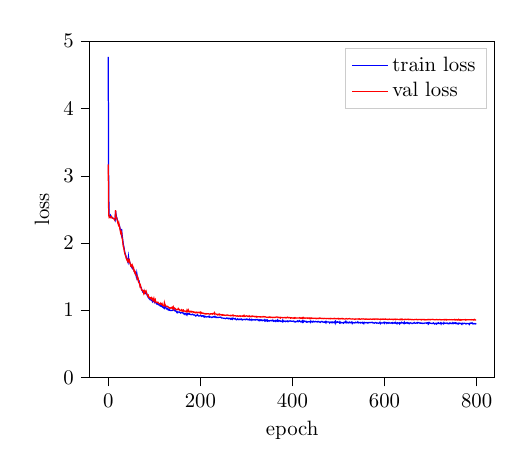
\begin{tikzpicture}[scale=0.75]

\definecolor{darkgray176}{RGB}{176,176,176}
\definecolor{lightgray204}{RGB}{204,204,204}

\begin{axis}[
legend cell align={left},
legend style={fill opacity=0.8, draw opacity=1, text opacity=1, draw=lightgray204},
tick align=outside,
tick pos=left,
x grid style={darkgray176},
xlabel={epoch},
xmin=-39.95, xmax=838.95,
xtick style={color=black},
y grid style={darkgray176},
ylabel={loss},
%ymin=0.590674677491188, ymax=4.96876869698366,
ymin=0, ymax=5,
ytick style={color=black}
]
\addplot [semithick, blue]
table {%
0 4.76976442337036
1 2.76665226618449
2 2.40345080693563
3 2.39860431353251
4 2.3923335870107
5 2.40936430295308
6 2.38829398155212
7 2.38435506820679
8 2.38447332382202
9 2.37373129526774
10 2.36964543660482
11 2.36714959144592
12 2.36331748962402
13 2.35865839322408
14 2.35167837142944
15 2.33851250012716
16 2.47256064414978
17 2.42310476303101
18 2.38571381568909
19 2.36909659703573
20 2.34048732121785
21 2.30845475196838
22 2.29311505953471
23 2.27155351638794
24 2.26730497678121
25 2.23956219355265
26 2.21051454544067
27 2.18204458554586
28 2.14430769284566
29 2.20875024795532
30 2.12511404355367
31 2.07468255360921
32 2.02139719327291
33 1.97205114364624
34 1.9458079735438
35 1.89684764544169
36 1.86404430866241
37 1.8383537530899
38 1.8145561615626
39 1.79469887415568
40 1.76952381928762
41 1.75038425127665
42 1.73122612635295
43 1.7122528553009
44 1.79318511486053
45 1.73858535289764
46 1.72663903236389
47 1.709352850914
48 1.69230484962463
49 1.65961726506551
50 1.65491263071696
51 1.63948043187459
52 1.62804293632507
53 1.6438064177831
54 1.63095696767171
55 1.60470028718313
56 1.59570701917013
57 1.56791055202484
58 1.56342418988546
59 1.53819489479065
60 1.52852694193522
61 1.49817037582397
62 1.55033544699351
63 1.50601736704508
64 1.49070306619008
65 1.45638064543406
66 1.424773534139
67 1.43273103237152
68 1.39125164349874
69 1.37673155466716
70 1.35270078976949
71 1.33887076377869
72 1.33206685384115
73 1.29925056298574
74 1.29199616114299
75 1.27355607350667
76 1.27840133508046
77 1.27362775802612
78 1.28487837314606
79 1.26797052224477
80 1.25294224421183
81 1.24914538860321
82 1.26787805557251
83 1.26505494117737
84 1.24016813437144
85 1.21637539068858
86 1.20573763052622
87 1.18758451938629
88 1.18470430374146
89 1.17246981461843
90 1.16837660471598
91 1.15667164325714
92 1.15633499622345
93 1.15347238381704
94 1.14739314715068
95 1.15268282095591
96 1.13254904747009
97 1.15191380182902
98 1.13184809684753
99 1.12989640235901
100 1.14132885138194
101 1.1149556239446
102 1.12092049916585
103 1.12311355272929
104 1.10943118731181
105 1.09467307726542
106 1.09148414929708
107 1.09669287999471
108 1.08991865317027
109 1.08154352506002
110 1.08434391021729
111 1.08313226699829
112 1.07422558466593
113 1.06255718072255
114 1.0660533507665
115 1.08238323529561
116 1.05755066871643
117 1.0529009103775
118 1.04708198706309
119 1.05060438315074
120 1.0376832485199
121 1.04410954316457
122 1.03204568227132
123 1.05512340863546
124 1.05555049578349
125 1.04498569170634
126 1.02203047275543
127 1.01890806357066
128 1.02835369110107
129 1.03022110462189
130 1.00776052474976
131 1.01179071267446
132 1.00229982535044
133 1.00806599855423
134 0.999489307403564
135 0.995865563551585
136 0.997665723164876
137 0.995976706345876
138 0.997372229894002
139 0.99676126241684
140 1.00315491358439
141 1.00270837545395
142 1.01822183529536
143 1.01069156328837
144 0.995511889457703
145 0.990767975648244
146 0.999321222305298
147 0.987883607546488
148 0.979580243428548
149 0.968295554320017
150 0.975632508595785
151 0.964838226636251
152 0.974176943302155
153 0.97488139073054
154 0.976079305013021
155 0.969716389973958
156 0.96608167886734
157 0.959330022335052
158 0.966760496298472
159 0.964924097061157
160 0.963963687419891
161 0.960572123527527
162 0.963602940241496
163 0.957162419954936
164 0.950136383374532
165 0.941254615783691
166 0.95301365852356
167 0.949311415354411
168 0.952055037021637
169 0.936202466487885
170 0.942308187484741
171 0.929663459459941
172 0.949082752068838
173 0.941849748293559
174 0.945329666137695
175 0.951742152372996
176 0.943045377731323
177 0.946065803368886
178 0.938916186491648
179 0.936445116996765
180 0.933801352977753
181 0.934804896513621
182 0.936628818511963
183 0.942484279473623
184 0.938362876574198
185 0.93024605512619
186 0.929862141609192
187 0.931658307711283
188 0.930023570855459
189 0.923292954762777
190 0.91381977001826
191 0.91742338736852
192 0.92475026845932
193 0.92959580818812
194 0.934653242429098
195 0.923009196917216
196 0.914671003818512
197 0.913694938023885
198 0.915326118469238
199 0.918788731098175
200 0.918506324291229
201 0.92487770318985
202 0.91642036040624
203 0.909264028072357
204 0.91490646203359
205 0.918348133563995
206 0.919907708962758
207 0.906235138575236
208 0.912376523017883
209 0.901341418425242
210 0.909709771474203
211 0.909180243810018
212 0.900647143522898
213 0.900256156921387
214 0.901325106620789
215 0.904896060625712
216 0.902408123016357
217 0.901297688484192
218 0.901953458786011
219 0.912313044071198
220 0.897025585174561
221 0.899534503618876
222 0.899145245552063
223 0.901484807332357
224 0.89237380027771
225 0.891325215498606
226 0.89508577187856
227 0.895942767461141
228 0.905863106250763
229 0.902073204517365
230 0.904415686925252
231 0.899457653363546
232 0.908758401870728
233 0.899115681648254
234 0.8914675116539
235 0.898094515005747
236 0.896493415037791
237 0.891352494557699
238 0.891367693742116
239 0.891834914684296
240 0.893989761670431
241 0.897189418474833
242 0.894818127155304
243 0.896941939989726
244 0.898073653380076
245 0.894978225231171
246 0.884364386399587
247 0.884100019931793
248 0.88425346215566
249 0.883714556694031
250 0.882189551989237
251 0.882084647814433
252 0.882616718610128
253 0.879366517066956
254 0.878558874130249
255 0.875147779782613
256 0.880608995755514
257 0.886251986026764
258 0.886002977689107
259 0.877920389175415
260 0.879564583301544
261 0.881602247556051
262 0.873117466767629
263 0.879893104235331
264 0.87895268201828
265 0.877017617225647
266 0.867618521054586
267 0.875859459241231
268 0.869847635428111
269 0.879067679246267
270 0.867780864238739
271 0.881360073884328
272 0.880498786767324
273 0.874673863252004
274 0.869985520839691
275 0.873778124650319
276 0.877751568953196
277 0.866170307000478
278 0.858366231123606
279 0.864339907964071
280 0.865037600199381
281 0.872375210126241
282 0.862059831619263
283 0.865753531455994
284 0.861452539761861
285 0.867580672105153
286 0.86306111017863
287 0.867127080758413
288 0.863437314828237
289 0.869584977626801
290 0.864792287349701
291 0.854810794194539
292 0.856271425882975
293 0.864179233709971
294 0.862010796864828
295 0.861558794975281
296 0.865249494711558
297 0.866008857885996
298 0.860599637031555
299 0.860369066397349
300 0.868428726991018
301 0.870777070522308
302 0.865216354529063
303 0.860049525896708
304 0.862078607082367
305 0.857807298501333
306 0.860143522421519
307 0.867055594921112
308 0.854136824607849
309 0.857420563697815
310 0.857826232910156
311 0.86360627412796
312 0.851279397805532
313 0.86141304175059
314 0.858164668083191
315 0.857060670852661
316 0.860290586948395
317 0.858681241671244
318 0.856054027875265
319 0.859415670235952
320 0.85489426056544
321 0.861599346001943
322 0.859688778718313
323 0.858375827471415
324 0.863613327344259
325 0.862518688042959
326 0.848451813062032
327 0.854497810204824
328 0.856197039286296
329 0.846717099348704
330 0.857442577679952
331 0.850810388724009
332 0.855995237827301
333 0.84870457649231
334 0.853327135245005
335 0.845882495244344
336 0.850425163904826
337 0.852515121301015
338 0.854137619336446
339 0.845664997895559
340 0.857501308123271
341 0.839705725510915
342 0.84624586502711
343 0.855059484640757
344 0.845406055450439
345 0.838748673597972
346 0.851996223131816
347 0.840264856815338
348 0.845167219638824
349 0.843728085358938
350 0.839146792888641
351 0.842441995938619
352 0.846170922120412
353 0.84600023428599
354 0.844913919766744
355 0.842836976051331
356 0.852481504281362
357 0.845485905806224
358 0.849095543225606
359 0.837088286876678
360 0.844026406606038
361 0.839608709017436
362 0.836946487426758
363 0.845020194848379
364 0.834767440954844
365 0.847219129403432
366 0.840891261895498
367 0.838756561279297
368 0.85444454352061
369 0.837222297986349
370 0.844637850920359
371 0.839489638805389
372 0.843287746111552
373 0.846605877081553
374 0.837905208269755
375 0.833404799302419
376 0.835303624471029
377 0.838701784610748
378 0.831317881743113
379 0.851682901382446
380 0.834012905756632
381 0.841213961442312
382 0.836928685506185
383 0.838220556577047
384 0.835889597733816
385 0.830978910128276
386 0.838492472966512
387 0.836636980374654
388 0.8370361328125
389 0.840688566366831
390 0.829596141974131
391 0.831176996231079
392 0.838809271653493
393 0.840492526690165
394 0.838912069797516
395 0.84268045425415
396 0.838532567024231
397 0.840665558973948
398 0.836423416932424
399 0.837258656819661
400 0.836765348911285
401 0.838338772455851
402 0.84124219417572
403 0.837805112202962
404 0.828240076700846
405 0.831453561782837
406 0.831571658452352
407 0.825932244459788
408 0.831980764865875
409 0.834135850270589
410 0.831852436065674
411 0.842366218566895
412 0.835994283358256
413 0.831279695034027
414 0.837624152501424
415 0.845300833384196
416 0.835285445054372
417 0.835334459940592
418 0.827387511730194
419 0.826530555884043
420 0.834989209969838
421 0.840416093667348
422 0.82605383793513
423 0.842174291610718
424 0.826043923695882
425 0.835110545158386
426 0.841056227684021
427 0.839925865332286
428 0.832233468691508
429 0.83379856745402
430 0.826274772485097
431 0.832929650942485
432 0.823215246200562
433 0.82416299978892
434 0.828157683213552
435 0.829493204752604
436 0.831718722979228
437 0.8298459649086
438 0.832108835379283
439 0.821248213450114
440 0.839411854743958
441 0.829466919104258
442 0.82693076133728
443 0.82344396909078
444 0.83289380868276
445 0.837564388910929
446 0.83088497320811
447 0.825890143712362
448 0.827909549077352
449 0.833417455355326
450 0.835137784481049
451 0.827937185764313
452 0.827293515205383
453 0.828795532385508
454 0.830724020799001
455 0.826347768306732
456 0.834119339783986
457 0.830323179562887
458 0.828697303930918
459 0.825818061828613
460 0.822012046972911
461 0.819668332735697
462 0.830308755238851
463 0.834701259930929
464 0.833331644535065
465 0.832582334677378
466 0.825390338897705
467 0.82144566377004
468 0.825759927431742
469 0.823217491308848
470 0.82713786760966
471 0.820428987344106
472 0.830268760522207
473 0.814653396606445
474 0.830817004044851
475 0.825029532114665
476 0.825354735056559
477 0.825648625691732
478 0.82573801279068
479 0.826870838801066
480 0.822031219800313
481 0.81095947821935
482 0.821307460467021
483 0.820556998252869
484 0.826553821563721
485 0.821294248104095
486 0.812929511070251
487 0.820832808812459
488 0.827151119709015
489 0.820954422156016
490 0.815938691298167
491 0.819966912269592
492 0.829169571399689
493 0.808328092098236
494 0.832478642463684
495 0.815939386685689
496 0.821467479070028
497 0.820669591426849
498 0.828077713648478
499 0.823160727818807
500 0.824233333269755
501 0.822930196921031
502 0.814908723036448
503 0.827524363994598
504 0.811874568462372
505 0.819673836231232
506 0.81594063838323
507 0.816849033037821
508 0.813368956247965
509 0.813068628311157
510 0.817183593908946
511 0.807532707850138
512 0.814564764499664
513 0.823911925156911
514 0.82303911447525
515 0.818194488684336
516 0.833719770113627
517 0.814166963100433
518 0.811846852302551
519 0.822493175665537
520 0.816717565059662
521 0.819854458173116
522 0.811526676019033
523 0.813556432723999
524 0.824001610279083
525 0.819526116053263
526 0.815482397874196
527 0.815117120742798
528 0.822528560956319
529 0.827293296655019
530 0.804657896359762
531 0.815871040026347
532 0.816313882668813
533 0.814098159472148
534 0.811825017134349
535 0.812263429164886
536 0.816550811131795
537 0.821204741795858
538 0.813914398352305
539 0.818714261054993
540 0.817079663276672
541 0.816830774148305
542 0.827441354592641
543 0.812528610229492
544 0.816635588804881
545 0.818234244982401
546 0.814129670461019
547 0.815752983093262
548 0.810861905415853
549 0.817729075749715
550 0.813421110312144
551 0.815907577673594
552 0.819979945818583
553 0.808004438877106
554 0.811498443285624
555 0.80234702428182
556 0.820146103700002
557 0.815799395243327
558 0.815734048684438
559 0.81548156340917
560 0.81813249985377
561 0.813723623752594
562 0.816356162230174
563 0.816070954004923
564 0.808086117108663
565 0.816424707571665
566 0.818436940511068
567 0.815997282663981
568 0.818158308664958
569 0.818657994270325
570 0.815855960051219
571 0.817346533139547
572 0.816686888535818
573 0.821922222773234
574 0.816719472408295
575 0.811024606227875
576 0.81320732831955
577 0.808865547180176
578 0.808302084604899
579 0.812106688817342
580 0.817880789438883
581 0.816519757111867
582 0.81597775220871
583 0.80838151772817
584 0.811761637528737
585 0.809053778648376
586 0.810812393824259
587 0.806744237740835
588 0.809285402297974
589 0.810849269231161
590 0.820698817571004
591 0.800978283087412
592 0.809801161289215
593 0.809612691402435
594 0.812545617421468
595 0.81326679388682
596 0.810442427794139
597 0.811133583386739
598 0.816460450490316
599 0.821845432122548
600 0.806925594806671
601 0.817602594693502
602 0.816967328389486
603 0.819211979707082
604 0.814522922039032
605 0.804856856664022
606 0.812441567579905
607 0.814801931381226
608 0.810371140638987
609 0.807249009609222
610 0.817370017369588
611 0.810630897680918
612 0.809379160404205
613 0.808559238910675
614 0.812226951122284
615 0.813091655572255
616 0.807076533635457
617 0.815610468387604
618 0.805885811646779
619 0.810390412807465
620 0.812814037005107
621 0.809595505396525
622 0.816958725452423
623 0.811676939328512
624 0.819065968195597
625 0.806854287783305
626 0.807556847731272
627 0.799391249815623
628 0.813991983731588
629 0.809236983458201
630 0.808793624242147
631 0.807888368765513
632 0.813394844532013
633 0.798724353313446
634 0.812472263971964
635 0.808660844961802
636 0.810146987438202
637 0.819946090380351
638 0.811652620633443
639 0.812595963478088
640 0.812508165836334
641 0.80819966395696
642 0.802838921546936
643 0.821883638699849
644 0.806759238243103
645 0.811718622843424
646 0.807935615380605
647 0.812096615632375
648 0.814985950787862
649 0.808687587579091
650 0.816717783610026
651 0.814435422420502
652 0.804136951764425
653 0.807413200537364
654 0.801271875699361
655 0.80926775932312
656 0.813807725906372
657 0.810865004857381
658 0.80917888879776
659 0.808257400989532
660 0.802045385042826
661 0.806507309277852
662 0.806370496749878
663 0.810981571674347
664 0.814755419890086
665 0.818111856778463
666 0.807862957318624
667 0.805873076121012
668 0.807369709014893
669 0.809336344401042
670 0.814034700393677
671 0.816885113716125
672 0.808592995007833
673 0.816211303075155
674 0.8130770723025
675 0.813619216283162
676 0.809879879156748
677 0.806907991568247
678 0.806188861529032
679 0.812426288922628
680 0.807357589403788
681 0.808357894420624
682 0.808640996615092
683 0.803012986977895
684 0.805473784605662
685 0.807667513688405
686 0.803839008013407
687 0.809622128804525
688 0.810243944327037
689 0.809967339038849
690 0.810096780459086
691 0.807205080986023
692 0.814001063505808
693 0.812196214993795
694 0.813284317652384
695 0.792570273081462
696 0.800326029459635
697 0.817392786343892
698 0.811438540617625
699 0.809336046377818
700 0.807505011558533
701 0.807185212771098
702 0.803679207960765
703 0.804517825444539
704 0.805149833361308
705 0.804774363835653
706 0.811529099941254
707 0.804365118344625
708 0.803009510040283
709 0.796957532564799
710 0.803945402304331
711 0.805393973986308
712 0.804871439933777
713 0.7957484126091
714 0.807941873868307
715 0.804819981257121
716 0.804276883602142
717 0.814444084962209
718 0.810358226299286
719 0.803216179211934
720 0.804355402787526
721 0.804875830809275
722 0.813040872414907
723 0.795466045538584
724 0.809214353561401
725 0.80696165561676
726 0.80509614944458
727 0.806869308153788
728 0.799949963887533
729 0.816396355628967
730 0.80775252978007
731 0.804289857546488
732 0.806604544321696
733 0.808317005634308
734 0.810109734535217
735 0.808650890986125
736 0.802610754966736
737 0.809369285901388
738 0.806261360645294
739 0.802043517430623
740 0.79850035905838
741 0.804410974184672
742 0.811351597309113
743 0.805258969465891
744 0.808048943678538
745 0.802461365858714
746 0.805187702178955
747 0.805482546488444
748 0.81368480126063
749 0.800822714964549
750 0.806379417578379
751 0.813133140405019
752 0.807602425416311
753 0.808712323506673
754 0.812647501627604
755 0.803001344203949
756 0.809859116872152
757 0.802487015724182
758 0.798302332560221
759 0.806537608305613
760 0.803798894087474
761 0.797228991985321
762 0.809974710146586
763 0.806241611639659
764 0.806646684805552
765 0.802393992741903
766 0.804718057314555
767 0.797230660915375
768 0.790535946687063
769 0.806430339813232
770 0.80209751923879
771 0.800008118152618
772 0.804043610890706
773 0.807645738124847
774 0.80539615948995
775 0.804212530454
776 0.804127295811971
777 0.796629369258881
778 0.802888115247091
779 0.802275737126668
780 0.80159189303716
781 0.802689810593923
782 0.802599231402079
783 0.80076938867569
784 0.789678951104482
785 0.804695049921672
786 0.810124099254608
787 0.805161654949188
788 0.80666571855545
789 0.808380126953125
790 0.813392738501231
791 0.800556143124898
792 0.804503858089447
793 0.80140761534373
794 0.796969711780548
795 0.797970136006673
796 0.803184469540914
797 0.799741506576538
798 0.796563486258189
799 0.80493289232254
};
\addlegendentry{train loss}
\addplot [semithick, red]
table {%
0 3.16941595077515
1 2.41605496406555
2 2.38436150550842
3 2.39684915542603
4 2.38500022888184
5 2.37620496749878
6 2.3754301071167
7 2.39122247695923
8 2.37548351287842
9 2.37098979949951
10 2.36919569969177
11 2.36593341827393
12 2.36266374588013
13 2.35748434066772
14 2.34436655044556
15 2.37042593955994
16 2.48748183250427
17 2.38647818565369
18 2.3789496421814
19 2.35405826568604
20 2.32618379592896
21 2.29714179039001
22 2.27439713478088
23 2.29801607131958
24 2.25751781463623
25 2.22342824935913
26 2.18863654136658
27 2.15460729598999
28 2.17312335968018
29 2.15686583518982
30 2.07649302482605
31 2.05147123336792
32 1.98679399490356
33 1.93900990486145
34 1.92359471321106
35 1.87717294692993
36 1.84372162818909
37 1.82122647762299
38 1.80560803413391
39 1.77419650554657
40 1.75869452953339
41 1.7437881231308
42 1.72962856292725
43 1.75443208217621
44 1.72003817558289
45 1.72427356243134
46 1.74193048477173
47 1.70766448974609
48 1.68726539611816
49 1.66009557247162
50 1.66650748252869
51 1.65443921089172
52 1.67605948448181
53 1.65794396400452
54 1.62121748924255
55 1.62912535667419
56 1.58500850200653
57 1.58899474143982
58 1.5538809299469
59 1.56251192092896
60 1.52412021160126
61 1.52333581447601
62 1.52150106430054
63 1.47322082519531
64 1.48757934570312
65 1.46595501899719
66 1.41577696800232
67 1.4143933057785
68 1.40156078338623
69 1.35781371593475
70 1.3713116645813
71 1.34104287624359
72 1.31294846534729
73 1.30237054824829
74 1.29331386089325
75 1.29384195804596
76 1.28520524501801
77 1.25759768486023
78 1.28703057765961
79 1.26184368133545
80 1.27997779846191
81 1.28443825244904
82 1.29133331775665
83 1.25649476051331
84 1.23433434963226
85 1.22557890415192
86 1.216313123703
87 1.22404623031616
88 1.19155168533325
89 1.1940153837204
90 1.19192266464233
91 1.17929100990295
92 1.18391108512878
93 1.16925120353699
94 1.18801879882812
95 1.17984092235565
96 1.17614078521729
97 1.14675652980804
98 1.15347909927368
99 1.1746631860733
100 1.13582372665405
101 1.15457093715668
102 1.1636209487915
103 1.13103270530701
104 1.11733615398407
105 1.12068033218384
106 1.12057983875275
107 1.1135470867157
108 1.11883187294006
109 1.10776925086975
110 1.10066151618958
111 1.09767937660217
112 1.09318947792053
113 1.09190738201141
114 1.10430431365967
115 1.08729672431946
116 1.08722674846649
117 1.09679210186005
118 1.07346224784851
119 1.07328736782074
120 1.07289838790894
121 1.06533777713776
122 1.11380648612976
123 1.08845961093903
124 1.07539439201355
125 1.06599497795105
126 1.05710685253143
127 1.05412781238556
128 1.05428326129913
129 1.05826532840729
130 1.0518434047699
131 1.04510295391083
132 1.0395519733429
133 1.03110575675964
134 1.0352874994278
135 1.03064560890198
136 1.03408825397491
137 1.0412403345108
138 1.03168630599976
139 1.02690708637238
140 1.04862344264984
141 1.05578434467316
142 1.02230584621429
143 1.03797471523285
144 1.03270792961121
145 1.0278400182724
146 1.02337861061096
147 1.00926947593689
148 1.00767421722412
149 1.00978600978851
150 1.00974178314209
151 1.00793051719666
152 1.02541136741638
153 1.012810587883
154 1.01429557800293
155 1.00204968452454
156 1.00058448314667
157 1.00063705444336
158 0.99294376373291
159 1.00676155090332
160 0.996167659759521
161 0.989984452724457
162 1.00354433059692
163 1.00556874275208
164 0.98615026473999
165 0.987772881984711
166 0.988092303276062
167 0.988455951213837
168 0.982214152812958
169 0.984500110149384
170 0.978541612625122
171 1.00022804737091
172 0.977459132671356
173 0.975743293762207
174 1.0018162727356
175 0.985277116298676
176 0.986008524894714
177 0.976234793663025
178 0.982417464256287
179 0.985003888607025
180 0.972867488861084
181 0.982702255249023
182 0.977900505065918
183 0.979881763458252
184 0.97375363111496
185 0.969328880310059
186 0.97558867931366
187 0.970858097076416
188 0.964957475662231
189 0.970008313655853
190 0.961764693260193
191 0.966552019119263
192 0.970869541168213
193 0.962548732757568
194 0.967639148235321
195 0.962809205055237
196 0.966112971305847
197 0.971071898937225
198 0.965074241161346
199 0.960777163505554
200 0.969626426696777
201 0.954131782054901
202 0.967188119888306
203 0.960058569908142
204 0.956149756908417
205 0.959278583526611
206 0.95268177986145
207 0.954565227031708
208 0.952821612358093
209 0.948505103588104
210 0.951637864112854
211 0.943968713283539
212 0.944578647613525
213 0.949016749858856
214 0.944922685623169
215 0.946992754936218
216 0.946696996688843
217 0.948660135269165
218 0.947592675685883
219 0.94488787651062
220 0.945104777812958
221 0.941632628440857
222 0.94788658618927
223 0.944168925285339
224 0.947579860687256
225 0.948440909385681
226 0.942693889141083
227 0.951373338699341
228 0.95412290096283
229 0.953903675079346
230 0.943627059459686
231 0.962165236473083
232 0.946067571640015
233 0.945003986358643
234 0.944278240203857
235 0.940838813781738
236 0.939560770988464
237 0.931997954845428
238 0.939363658428192
239 0.934359550476074
240 0.939845740795135
241 0.931941866874695
242 0.942348122596741
243 0.936964511871338
244 0.932930827140808
245 0.935157239437103
246 0.934256970882416
247 0.926840722560883
248 0.933125019073486
249 0.927037239074707
250 0.926878154277802
251 0.931482911109924
252 0.930071473121643
253 0.924359917640686
254 0.925539255142212
255 0.92324560880661
256 0.922662675380707
257 0.928386151790619
258 0.930880427360535
259 0.927241504192352
260 0.922896981239319
261 0.925397396087646
262 0.922937273979187
263 0.923870444297791
264 0.923107743263245
265 0.917245388031006
266 0.92419159412384
267 0.922355532646179
268 0.919834971427917
269 0.923244833946228
270 0.927926540374756
271 0.918496966362
272 0.924658060073853
273 0.916705250740051
274 0.918478429317474
275 0.916970133781433
276 0.916570901870728
277 0.917524516582489
278 0.912591695785522
279 0.915456295013428
280 0.913101077079773
281 0.917579174041748
282 0.914037466049194
283 0.910103797912598
284 0.912255167961121
285 0.915648877620697
286 0.918298840522766
287 0.908679246902466
288 0.913011252880096
289 0.913279891014099
290 0.912468433380127
291 0.912914276123047
292 0.912143588066101
293 0.918760180473328
294 0.911503553390503
295 0.922639727592468
296 0.909883260726929
297 0.913041532039642
298 0.909648299217224
299 0.91387814283371
300 0.916758418083191
301 0.914790868759155
302 0.915411412715912
303 0.906774163246155
304 0.908764958381653
305 0.908266544342041
306 0.918216943740845
307 0.911168277263641
308 0.903289973735809
309 0.909791171550751
310 0.906640470027924
311 0.911604642868042
312 0.906807124614716
313 0.913787007331848
314 0.912986874580383
315 0.909299373626709
316 0.911193549633026
317 0.909083068370819
318 0.904710650444031
319 0.906525135040283
320 0.903680562973022
321 0.909697711467743
322 0.89948433637619
323 0.902014672756195
324 0.90138167142868
325 0.90541398525238
326 0.90410041809082
327 0.90366518497467
328 0.903528928756714
329 0.902599215507507
330 0.898125112056732
331 0.902363777160645
332 0.90216326713562
333 0.901420116424561
334 0.899225890636444
335 0.90099024772644
336 0.906487643718719
337 0.90221118927002
338 0.906682372093201
339 0.902254819869995
340 0.901032328605652
341 0.902995347976685
342 0.900126338005066
343 0.897629380226135
344 0.89552104473114
345 0.896450161933899
346 0.896890819072723
347 0.89386522769928
348 0.898286044597626
349 0.893290042877197
350 0.895949065685272
351 0.90234512090683
352 0.89380669593811
353 0.893132090568542
354 0.895838737487793
355 0.895293593406677
356 0.893720328807831
357 0.891225278377533
358 0.896243572235107
359 0.892247080802917
360 0.89090633392334
361 0.89465868473053
362 0.895645380020142
363 0.893460273742676
364 0.895033299922943
365 0.899394154548645
366 0.900723099708557
367 0.900758922100067
368 0.895417094230652
369 0.89643520116806
370 0.895093858242035
371 0.888822555541992
372 0.888764142990112
373 0.894596576690674
374 0.885004460811615
375 0.891944289207458
376 0.891334056854248
377 0.892224669456482
378 0.893210351467133
379 0.887716472148895
380 0.890780568122864
381 0.889793157577515
382 0.890191256999969
383 0.892045438289642
384 0.889963388442993
385 0.890876054763794
386 0.885559320449829
387 0.88893860578537
388 0.892471432685852
389 0.896901965141296
390 0.890807330608368
391 0.892667412757874
392 0.888192415237427
393 0.892359495162964
394 0.891262888908386
395 0.888161659240723
396 0.881853044033051
397 0.887596964836121
398 0.884378135204315
399 0.887709856033325
400 0.884670972824097
401 0.883210778236389
402 0.8861985206604
403 0.881826102733612
404 0.888974070549011
405 0.88233757019043
406 0.889323234558105
407 0.883536994457245
408 0.882926404476166
409 0.884847640991211
410 0.885902583599091
411 0.886532247066498
412 0.883718430995941
413 0.884906411170959
414 0.884892463684082
415 0.887815237045288
416 0.890766799449921
417 0.882901191711426
418 0.885289669036865
419 0.880347013473511
420 0.881796360015869
421 0.889599561691284
422 0.878255844116211
423 0.883241832256317
424 0.890621662139893
425 0.882128179073334
426 0.881797909736633
427 0.885832786560059
428 0.881942272186279
429 0.884105682373047
430 0.883119702339172
431 0.883985638618469
432 0.881930530071259
433 0.885581374168396
434 0.880369365215302
435 0.883298873901367
436 0.88334321975708
437 0.885696411132812
438 0.875640988349915
439 0.883685827255249
440 0.875894069671631
441 0.880963742733002
442 0.88541454076767
443 0.88106107711792
444 0.880634069442749
445 0.87882125377655
446 0.879933536052704
447 0.879703223705292
448 0.882618367671967
449 0.882545173168182
450 0.878006160259247
451 0.880003571510315
452 0.87523353099823
453 0.87974750995636
454 0.879966974258423
455 0.876713991165161
456 0.877361416816711
457 0.876095950603485
458 0.884492635726929
459 0.8798668384552
460 0.883754253387451
461 0.881622672080994
462 0.876672923564911
463 0.876393973827362
464 0.880432069301605
465 0.87920606136322
466 0.876517713069916
467 0.875315546989441
468 0.878304183483124
469 0.880428969860077
470 0.877849936485291
471 0.878861784934998
472 0.877960920333862
473 0.877035856246948
474 0.874886214733124
475 0.879011273384094
476 0.878521323204041
477 0.879117965698242
478 0.878711462020874
479 0.873833835124969
480 0.876862227916718
481 0.877071261405945
482 0.872943878173828
483 0.878913044929504
484 0.877578675746918
485 0.877431333065033
486 0.873699843883514
487 0.874722838401794
488 0.877472281455994
489 0.875276327133179
490 0.875998139381409
491 0.879260778427124
492 0.873154282569885
493 0.875407099723816
494 0.876748204231262
495 0.875693023204803
496 0.873281717300415
497 0.876521110534668
498 0.87740820646286
499 0.873544216156006
500 0.877742409706116
501 0.869556784629822
502 0.87425297498703
503 0.87637060880661
504 0.87583315372467
505 0.872168064117432
506 0.875971019268036
507 0.875990331172943
508 0.872417688369751
509 0.877622246742249
510 0.87378853559494
511 0.872901201248169
512 0.870694100856781
513 0.87181293964386
514 0.871402621269226
515 0.87118399143219
516 0.873851478099823
517 0.877646803855896
518 0.873293340206146
519 0.870188593864441
520 0.869548976421356
521 0.872468948364258
522 0.872158288955688
523 0.873076438903809
524 0.876816272735596
525 0.874219655990601
526 0.871546626091003
527 0.869927406311035
528 0.868435621261597
529 0.868673205375671
530 0.86902779340744
531 0.872638702392578
532 0.869348466396332
533 0.870266199111938
534 0.869415938854218
535 0.864869475364685
536 0.868583619594574
537 0.867521286010742
538 0.871416926383972
539 0.86892694234848
540 0.869867503643036
541 0.87143075466156
542 0.869366645812988
543 0.871799409389496
544 0.867676973342896
545 0.867920637130737
546 0.872304081916809
547 0.86656928062439
548 0.867766320705414
549 0.868566751480103
550 0.868587732315063
551 0.872394442558289
552 0.869109332561493
553 0.869640231132507
554 0.871956348419189
555 0.870847940444946
556 0.868862509727478
557 0.866648554801941
558 0.868966102600098
559 0.866190671920776
560 0.870739340782166
561 0.869111001491547
562 0.866905808448792
563 0.868709325790405
564 0.867690682411194
565 0.866494834423065
566 0.868539333343506
567 0.867400050163269
568 0.866578936576843
569 0.870373725891113
570 0.870607018470764
571 0.867091596126556
572 0.867841362953186
573 0.866336941719055
574 0.868126273155212
575 0.867098689079285
576 0.871165931224823
577 0.869145572185516
578 0.864486217498779
579 0.870849549770355
580 0.868954181671143
581 0.868110299110413
582 0.869426131248474
583 0.869816243648529
584 0.863523960113525
585 0.870489478111267
586 0.869886040687561
587 0.867906987667084
588 0.865477323532104
589 0.866920948028564
590 0.86789482831955
591 0.86133348941803
592 0.86867368221283
593 0.868320643901825
594 0.866555631160736
595 0.867507338523865
596 0.869372546672821
597 0.86544406414032
598 0.868646562099457
599 0.865955591201782
600 0.868494510650635
601 0.865976929664612
602 0.87068510055542
603 0.866957545280457
604 0.865205943584442
605 0.86720198392868
606 0.867507815361023
607 0.861128211021423
608 0.86585009098053
609 0.862280309200287
610 0.86567485332489
611 0.868774771690369
612 0.866209924221039
613 0.864649653434753
614 0.864186644554138
615 0.865026473999023
616 0.866556763648987
617 0.863753020763397
618 0.866193473339081
619 0.860568761825562
620 0.867481231689453
621 0.866730213165283
622 0.864972710609436
623 0.868594646453857
624 0.860522389411926
625 0.865875601768494
626 0.864208579063416
627 0.865209937095642
628 0.866900682449341
629 0.863218724727631
630 0.864090442657471
631 0.863316893577576
632 0.860875070095062
633 0.86547178030014
634 0.861796498298645
635 0.867001295089722
636 0.860445618629456
637 0.86161482334137
638 0.868501603603363
639 0.859958648681641
640 0.861569166183472
641 0.861268520355225
642 0.863844037055969
643 0.865247011184692
644 0.860778987407684
645 0.865069389343262
646 0.865480840206146
647 0.863876342773438
648 0.863075435161591
649 0.864595413208008
650 0.864915072917938
651 0.865309715270996
652 0.862004220485687
653 0.867004036903381
654 0.863564252853394
655 0.861326098442078
656 0.864250302314758
657 0.862307548522949
658 0.861153841018677
659 0.859419703483582
660 0.863314807415009
661 0.861951351165771
662 0.86050820350647
663 0.860176742076874
664 0.859207391738892
665 0.862413287162781
666 0.861438393592834
667 0.863277554512024
668 0.862906217575073
669 0.861818909645081
670 0.865901589393616
671 0.860252976417542
672 0.860505044460297
673 0.86048424243927
674 0.863377690315247
675 0.862180471420288
676 0.861197471618652
677 0.86348956823349
678 0.863933444023132
679 0.861144661903381
680 0.85573148727417
681 0.862466096878052
682 0.861479461193085
683 0.861584663391113
684 0.860269665718079
685 0.862036883831024
686 0.859841108322144
687 0.862572193145752
688 0.855595111846924
689 0.859363436698914
690 0.860766649246216
691 0.860079944133759
692 0.85781466960907
693 0.86225962638855
694 0.860195517539978
695 0.860107898712158
696 0.864228129386902
697 0.862974286079407
698 0.863303065299988
699 0.856988549232483
700 0.862247169017792
701 0.862213551998138
702 0.860892534255981
703 0.861069619655609
704 0.863004326820374
705 0.864814877510071
706 0.860981583595276
707 0.860552668571472
708 0.859209895133972
709 0.860697209835052
710 0.860296726226807
711 0.860297858715057
712 0.860939919948578
713 0.863921046257019
714 0.85942530632019
715 0.860747516155243
716 0.859874248504639
717 0.8576700091362
718 0.860194087028503
719 0.862067401409149
720 0.861065566539764
721 0.859074532985687
722 0.860581517219543
723 0.856456398963928
724 0.858594298362732
725 0.859205007553101
726 0.857748031616211
727 0.860213220119476
728 0.860046863555908
729 0.861558198928833
730 0.856736660003662
731 0.862295508384705
732 0.859781384468079
733 0.861670613288879
734 0.855922818183899
735 0.862863540649414
736 0.860269010066986
737 0.860048711299896
738 0.858679711818695
739 0.859297215938568
740 0.858627438545227
741 0.860522508621216
742 0.857273578643799
743 0.857635676860809
744 0.858134388923645
745 0.857569873332977
746 0.860361516475677
747 0.857621610164642
748 0.860042750835419
749 0.858325004577637
750 0.859007775783539
751 0.858541011810303
752 0.863702535629272
753 0.856002688407898
754 0.859875559806824
755 0.855737149715424
756 0.861934065818787
757 0.858389616012573
758 0.854431390762329
759 0.858508825302124
760 0.859453320503235
761 0.865336060523987
762 0.854889094829559
763 0.85838907957077
764 0.853939652442932
765 0.86033833026886
766 0.853568196296692
767 0.858223557472229
768 0.855992078781128
769 0.860419750213623
770 0.860183894634247
771 0.858750462532043
772 0.859380424022675
773 0.85732889175415
774 0.858475625514984
775 0.862168550491333
776 0.853886961936951
777 0.859028995037079
778 0.856952905654907
779 0.857420444488525
780 0.857403218746185
781 0.858605265617371
782 0.857553660869598
783 0.858450531959534
784 0.859838664531708
785 0.858865022659302
786 0.857734799385071
787 0.857927918434143
788 0.856552839279175
789 0.861042380332947
790 0.858120620250702
791 0.858291327953339
792 0.857007384300232
793 0.859375655651093
794 0.85496187210083
795 0.864582419395447
796 0.859966695308685
797 0.8565514087677
798 0.857019066810608
799 0.856411457061768
};
\addlegendentry{val loss}
\end{axis}

\end{tikzpicture}

			\caption{Module 1: $\beta=0$}
		\end{subfigure}
		\hfill
		\begin{subfigure}[b]{0.45\textwidth}
			\centering
			% This file was created with tikzplotlib v0.10.1.
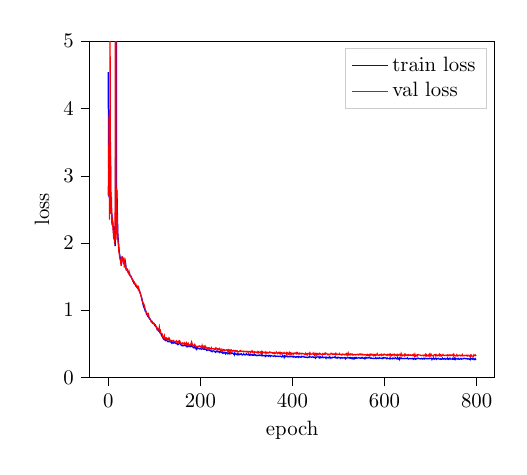
\begin{tikzpicture}[scale=0.75]

\definecolor{darkgray176}{RGB}{176,176,176}
\definecolor{lightgray204}{RGB}{204,204,204}

\begin{axis}[
legend cell align={left},
legend style={fill opacity=0.8, draw opacity=1, text opacity=1, draw=lightgray204},
tick align=outside,
tick pos=left,
x grid style={darkgray176},
xlabel={epoch},
xmin=-39.95, xmax=838.95,
xtick style={color=black},
y grid style={darkgray176},
ylabel={loss},
%ymin=-0.979698823392391, ymax=26.44131000489,
ymin=0, ymax=5,
ytick style={color=black}
]
\addplot [semithick, blue]
table {%
0 4.53948799769084
1 2.88770953814189
2 2.67463072141012
3 2.93288230895996
4 3.91456874211629
5 3.30372071266174
6 2.59048016866048
7 2.44383192062378
8 2.42939901351929
9 2.34263769785563
10 2.30482109387716
11 2.20496765772502
12 2.12699476877848
13 2.2483008702596
14 2.10834562778473
15 1.95365138848623
16 2.18112393220266
17 17.2476250330607
18 2.31542627016703
19 2.78638537724813
20 2.39792704582214
21 2.12750140825907
22 2.02488803863525
23 1.95284736156464
24 1.86275772253672
25 1.82302951812744
26 1.78187735875448
27 1.73974009354909
28 1.69182407855988
29 1.68986280759176
30 1.78630097707113
31 1.78862861792247
32 1.75306073824565
33 1.73894886175791
34 1.73672982056936
35 1.73612101872762
36 1.65905837217967
37 1.72588924566905
38 1.69069755077362
39 1.61700956026713
40 1.60132972399394
41 1.60905500253042
42 1.58714393774668
43 1.56331169605255
44 1.55317449569702
45 1.55380745728811
46 1.55950085322062
47 1.52922940254211
48 1.50636518001556
49 1.50150990486145
50 1.48993623256683
51 1.47828757762909
52 1.46258628368378
53 1.44218587875366
54 1.42592978477478
55 1.4223202864329
56 1.39950756231944
57 1.40089027086894
58 1.38984660307566
59 1.38831639289856
60 1.35973517100016
61 1.36080729961395
62 1.34569485982259
63 1.3347442150116
64 1.34080982208252
65 1.32535700003306
66 1.31568423906962
67 1.3038907845815
68 1.29028844833374
69 1.26890858014425
70 1.240003546079
71 1.21935506661733
72 1.20272262891134
73 1.17780447006226
74 1.14892566204071
75 1.1127032438914
76 1.07359449068705
77 1.05442309379578
78 1.03366100788116
79 1.02744126319885
80 0.990268429120382
81 0.985787252585093
82 0.978374739487966
83 0.943099757035573
84 0.941548407077789
85 0.920351346333822
86 0.909278213977814
87 0.902020374933879
88 0.893632829189301
89 0.881775180498759
90 0.869250317414602
91 0.871015727519989
92 0.856479585170746
93 0.839227159818014
94 0.824966609477997
95 0.832644899686178
96 0.813762346903483
97 0.804550290107727
98 0.803719858328501
99 0.807139774163564
100 0.798479000727336
101 0.77525136868159
102 0.780148009459178
103 0.759419322013855
104 0.752535879611969
105 0.735940376917521
106 0.716498633225759
107 0.724746267000834
108 0.702390313148499
109 0.694720606009165
110 0.703325867652893
111 0.685107092062632
112 0.690911471843719
113 0.656351745128632
114 0.655907293160756
115 0.641389707724253
116 0.621177613735199
117 0.621331691741943
118 0.595026950041453
119 0.597950100898743
120 0.573255022366842
121 0.565656105677287
122 0.561758637428284
123 0.574262221654256
124 0.567902525266012
125 0.548972904682159
126 0.553605874379476
127 0.562828560670217
128 0.553737680117289
129 0.537735899289449
130 0.531555076440175
131 0.536412596702576
132 0.541952133178711
133 0.545408348242442
134 0.530200203259786
135 0.528615057468414
136 0.526443501313527
137 0.530404567718506
138 0.512025703986486
139 0.519981722036997
140 0.516166647275289
141 0.511578559875488
142 0.523741066455841
143 0.516044358412425
144 0.514224310715993
145 0.524090190728505
146 0.519355634848277
147 0.506355077028275
148 0.505655348300934
149 0.500269442796707
150 0.506474713484446
151 0.488390525182088
152 0.490633388360341
153 0.496255666017532
154 0.501800288756688
155 0.516832103331884
156 0.50674295425415
157 0.497073849042257
158 0.486066391070684
159 0.477165877819061
160 0.47989030679067
161 0.470495045185089
162 0.470917503039042
163 0.475565175215403
164 0.473379621903102
165 0.475693861643473
166 0.484518229961395
167 0.473903208971024
168 0.479489713907242
169 0.471410046021144
170 0.466393748919169
171 0.457572142283122
172 0.470249394575755
173 0.460733989874522
174 0.459639509518941
175 0.462863256533941
176 0.4599695901076
177 0.471885701020559
178 0.469381332397461
179 0.459057112534841
180 0.46047979593277
181 0.478158334891001
182 0.46861923734347
183 0.462706128756205
184 0.449271341164907
185 0.441595127185186
186 0.442227989435196
187 0.457679212093353
188 0.445750057697296
189 0.459241578976313
190 0.434703201055527
191 0.421387414137522
192 0.443333605925242
193 0.429996649424235
194 0.442966302235921
195 0.433477222919464
196 0.431089748938878
197 0.432914276917775
198 0.429611335198085
199 0.424264639616013
200 0.432196150223414
201 0.430172820885976
202 0.423691729704539
203 0.419351726770401
204 0.42971995472908
205 0.441946536302567
206 0.430967499812444
207 0.423429588476817
208 0.431197712818782
209 0.418874512116114
210 0.422141303618749
211 0.417621165513992
212 0.421870112419128
213 0.417847623427709
214 0.402548919121424
215 0.405465831359227
216 0.410519460837046
217 0.409306108951569
218 0.408765266338984
219 0.404883911212285
220 0.404805292685827
221 0.398862332105637
222 0.402460922797521
223 0.407820026079814
224 0.388109902540843
225 0.39041926463445
226 0.384704907735189
227 0.394741137822469
228 0.398534625768661
229 0.393898685773214
230 0.392139772574107
231 0.39166921377182
232 0.37931963801384
233 0.375502397616704
234 0.385590275128682
235 0.391959557930628
236 0.383868714173635
237 0.381876160701116
238 0.381184031565984
239 0.38033327460289
240 0.38675511876742
241 0.386121640602748
242 0.373773455619812
243 0.385412067174911
244 0.392321934302648
245 0.377941499153773
246 0.373795588811239
247 0.376821796099345
248 0.36597220102946
249 0.377735912799835
250 0.37107507387797
251 0.362462361653646
252 0.370104730129242
253 0.368949254353841
254 0.366052637497584
255 0.352212617794673
256 0.367070347070694
257 0.366146673758825
258 0.366831163565318
259 0.362407843271891
260 0.350597947835922
261 0.354889094829559
262 0.366121053695679
263 0.37209074695905
264 0.352374732494354
265 0.35612819592158
266 0.356103748083115
267 0.364496072133382
268 0.357682595650355
269 0.363562395175298
270 0.363007436196009
271 0.357978711525599
272 0.35052889585495
273 0.357575178146362
274 0.339599072933197
275 0.36449858546257
276 0.348209222157796
277 0.348753343025843
278 0.341236899296443
279 0.34175435702006
280 0.355559855699539
281 0.341264188289642
282 0.350727995236715
283 0.351436972618103
284 0.338848928610484
285 0.348265171051025
286 0.34429873029391
287 0.344159990549088
288 0.351983765761058
289 0.351658413807551
290 0.344183842341105
291 0.334718306859334
292 0.337429066499074
293 0.341444273789724
294 0.350413332382838
295 0.344313780466716
296 0.343293974796931
297 0.334612687428792
298 0.33829739689827
299 0.34518293539683
300 0.355826914310455
301 0.347163498401642
302 0.337744931379954
303 0.336674690246582
304 0.339896996815999
305 0.348200817902883
306 0.333919793367386
307 0.342218528191249
308 0.332258075475693
309 0.341335554917653
310 0.343146204948425
311 0.34199055035909
312 0.332565893729528
313 0.330586075782776
314 0.336056808630625
315 0.33207901318868
316 0.332801173130671
317 0.346315900484721
318 0.332747588555018
319 0.329352607329686
320 0.335850735505422
321 0.329905649026235
322 0.330660700798035
323 0.323571056127548
324 0.331749906142553
325 0.330520570278168
326 0.329078604777654
327 0.327576150496801
328 0.334489285945892
329 0.328974554936091
330 0.329089850187302
331 0.327961315711339
332 0.335133423407872
333 0.33912718296051
334 0.323414524396261
335 0.330655346314112
336 0.323807249466578
337 0.322373578945796
338 0.327869236469269
339 0.327407608429591
340 0.32826492190361
341 0.310558100541433
342 0.313703487316767
343 0.331015825271606
344 0.326503068208694
345 0.322755217552185
346 0.322501838207245
347 0.320282638072968
348 0.316132416327794
349 0.330137153466543
350 0.32577183842659
351 0.329250117142995
352 0.315239717562993
353 0.322586516539256
354 0.32315390308698
355 0.3219180504481
356 0.319665461778641
357 0.318858583768209
358 0.319157948096593
359 0.314782659212748
360 0.321150650580724
361 0.322169572114944
362 0.319865266482035
363 0.320765902598699
364 0.312201956907908
365 0.318227996428808
366 0.314655184745789
367 0.314142684141795
368 0.317597230275472
369 0.315190037091573
370 0.315412769714991
371 0.312971731026967
372 0.314089069763819
373 0.317950228850047
374 0.314770231644313
375 0.313470284144084
376 0.309309442838033
377 0.305143266916275
378 0.314597318569819
379 0.328621158997218
380 0.315287937720617
381 0.314576894044876
382 0.298459341128667
383 0.321111649274826
384 0.313122610251109
385 0.309155066808065
386 0.319102505842845
387 0.31497997045517
388 0.319760779539744
389 0.316596974929174
390 0.305808484554291
391 0.308335820833842
392 0.312398155530294
393 0.308611919482549
394 0.309498101472855
395 0.31645921866099
396 0.308306147654851
397 0.308908671140671
398 0.313078949848811
399 0.316948016484578
400 0.311846991380056
401 0.306414395570755
402 0.31404854853948
403 0.304921487967173
404 0.311821003754934
405 0.31174173951149
406 0.304750670989354
407 0.300245056549708
408 0.30566617846489
409 0.309111088514328
410 0.303754438956579
411 0.309906542301178
412 0.310131112734477
413 0.301388879617055
414 0.312425235907237
415 0.306210974852244
416 0.305246224006017
417 0.304278115431468
418 0.302195866902669
419 0.314028700192769
420 0.306152025858561
421 0.311656415462494
422 0.309798985719681
423 0.311016192038854
424 0.307863424221675
425 0.312083045641581
426 0.304442822933197
427 0.301601032416026
428 0.301419834295909
429 0.304448703924815
430 0.300993879636129
431 0.29970379670461
432 0.298051029443741
433 0.295657455921173
434 0.301099489132563
435 0.304839164018631
436 0.299220085144043
437 0.309503118197123
438 0.311343133449554
439 0.305012941360474
440 0.305698484182358
441 0.302909086147944
442 0.300835152467092
443 0.305066287517548
444 0.308030813932419
445 0.307677547136943
446 0.299058159192403
447 0.30174528559049
448 0.298027902841568
449 0.300067663192749
450 0.288758764664332
451 0.303666343291601
452 0.300045907497406
453 0.306225270032883
454 0.307312071323395
455 0.305071920156479
456 0.306908915440242
457 0.305551995833715
458 0.293467432260513
459 0.303187310695648
460 0.293627113103867
461 0.306390384833018
462 0.300503939390182
463 0.296259095271428
464 0.298020233710607
465 0.307252238194148
466 0.29566153883934
467 0.29546794295311
468 0.301487565040588
469 0.302446921666463
470 0.298120747009913
471 0.302122493584951
472 0.296420176823934
473 0.284623225529989
474 0.299947122732798
475 0.294344355662664
476 0.298458009958267
477 0.295954237381617
478 0.291731476783752
479 0.300826569398244
480 0.298093577226003
481 0.3079920510451
482 0.287712295850118
483 0.297282040119171
484 0.29712634285291
485 0.291857133309046
486 0.291446973880132
487 0.296189546585083
488 0.302171111106873
489 0.299892803033193
490 0.297228187322617
491 0.29673778017362
492 0.304278284311295
493 0.295558661222458
494 0.303823053836823
495 0.295796126127243
496 0.292862892150879
497 0.287299027045568
498 0.296802630027135
499 0.30202646056811
500 0.293294807275136
501 0.293434182802836
502 0.293815056482951
503 0.295910477638245
504 0.285529394944509
505 0.292919804652532
506 0.290646404027939
507 0.294998486836751
508 0.2894260485967
509 0.294185092051824
510 0.291236460208893
511 0.289648761351903
512 0.291574428478877
513 0.296035130818685
514 0.292992681264877
515 0.280168851216634
516 0.29347304503123
517 0.286788235108058
518 0.290393819411596
519 0.289692183335622
520 0.293695598840714
521 0.296959161758423
522 0.29378883043925
523 0.287893225749334
524 0.296416491270065
525 0.299070666233699
526 0.287962863842646
527 0.291051536798477
528 0.283718238274256
529 0.290019631385803
530 0.283377041419347
531 0.292242695887883
532 0.278768360614777
533 0.290704369544983
534 0.292660633722941
535 0.282461096843084
536 0.29640793800354
537 0.286974320809046
538 0.288280208905538
539 0.295871734619141
540 0.286449094613393
541 0.289173712333043
542 0.291839281717936
543 0.291433016459147
544 0.29505314429601
545 0.291893382867177
546 0.290592461824417
547 0.286303540070852
548 0.287680784861247
549 0.29262962937355
550 0.289371798435847
551 0.299876431624095
552 0.297494957844416
553 0.286863565444946
554 0.289744367202123
555 0.285452634096146
556 0.289563457171122
557 0.280989398558935
558 0.295820454756419
559 0.282843798398972
560 0.287829051415126
561 0.291168570518494
562 0.295402546723684
563 0.290682007869085
564 0.289315402507782
565 0.291673094034195
566 0.298030316829681
567 0.293157299359639
568 0.293808331092199
569 0.286751101414363
570 0.285835931698481
571 0.290963461001714
572 0.286541044712067
573 0.286393900712331
574 0.284917304913203
575 0.281918505827586
576 0.285952170689901
577 0.283503393332164
578 0.281979829072952
579 0.284850110610326
580 0.284720371166865
581 0.292418410380681
582 0.280746668577194
583 0.286860764026642
584 0.284685631593068
585 0.290128439664841
586 0.290395855903625
587 0.282174716393153
588 0.283083558082581
589 0.294425169626872
590 0.289621114730835
591 0.288045366605123
592 0.286575744549433
593 0.284016450246175
594 0.282045801480611
595 0.289748052755992
596 0.280931582053502
597 0.282961338758469
598 0.296112944682439
599 0.296817312637965
600 0.29089746872584
601 0.289010832707087
602 0.292537877957026
603 0.288446575403214
604 0.287243713935216
605 0.279957850774129
606 0.288805733124415
607 0.281125068664551
608 0.28094807267189
609 0.28324634830157
610 0.282788395881653
611 0.278914699951808
612 0.294498999913534
613 0.27937321861585
614 0.283840179443359
615 0.283967971801758
616 0.282523393630981
617 0.278260231018066
618 0.290602634350459
619 0.291031489769618
620 0.281761318445206
621 0.279376556475957
622 0.287000338236491
623 0.289368043343226
624 0.292002658049266
625 0.28133217493693
626 0.277826895316442
627 0.28048187494278
628 0.291581273078918
629 0.278218100468318
630 0.283959666887919
631 0.275168319543203
632 0.289822657903035
633 0.270001788934072
634 0.290949374437332
635 0.290466487407684
636 0.283714781204859
637 0.289385636647542
638 0.281845778226852
639 0.281804541746775
640 0.28063307205836
641 0.283980558315913
642 0.281050304571788
643 0.282506148020426
644 0.280801653862
645 0.285148143768311
646 0.28259402513504
647 0.281075537204742
648 0.284341583649317
649 0.282328327496846
650 0.290550162394841
651 0.278681933879852
652 0.274778733650843
653 0.277208119630814
654 0.282190094391505
655 0.284078419208527
656 0.282113929589589
657 0.278598248958588
658 0.282673368851344
659 0.27840585509936
660 0.277589877446492
661 0.285474826892217
662 0.283581753571828
663 0.272316108147303
664 0.281670868396759
665 0.287437955538432
666 0.278454800446828
667 0.271900047858556
668 0.280715862909953
669 0.275974233945211
670 0.279899020989736
671 0.284841666618983
672 0.283304184675217
673 0.288720399141312
674 0.281651109457016
675 0.281980117162069
676 0.279811441898346
677 0.279206405083338
678 0.280354410409927
679 0.276436318953832
680 0.284801085789998
681 0.284398367007573
682 0.276835213104884
683 0.274253537257512
684 0.278127958377202
685 0.285962164402008
686 0.279455820719401
687 0.275820344686508
688 0.286625683307648
689 0.28095347682635
690 0.281051635742188
691 0.280194580554962
692 0.278153429428736
693 0.281161477168401
694 0.280301153659821
695 0.278937210639318
696 0.27797790368398
697 0.280895501375198
698 0.284729311863581
699 0.284594476222992
700 0.282347778479258
701 0.283860802650452
702 0.285506188869476
703 0.267765780289968
704 0.28036363919576
705 0.279469798008601
706 0.289695511261622
707 0.277536650498708
708 0.281989733378092
709 0.272992064555486
710 0.281509021917979
711 0.28941219051679
712 0.286735425392787
713 0.272395809491475
714 0.279970079660416
715 0.280883312225342
716 0.278766771157583
717 0.285680741071701
718 0.281361262003581
719 0.274201224247615
720 0.273058881362279
721 0.271358882387479
722 0.278731207052867
723 0.275298486153285
724 0.271157761414846
725 0.276231487592061
726 0.287084728479385
727 0.278718690077464
728 0.273791631062826
729 0.277662356694539
730 0.280407349268595
731 0.284687946240107
732 0.271125684181849
733 0.276832093795141
734 0.275855342547099
735 0.277605046828588
736 0.274099429448446
737 0.286700258652369
738 0.275052855412165
739 0.270101815462112
740 0.278865993022919
741 0.277193774779638
742 0.287041306495667
743 0.276187886794408
744 0.273393342892329
745 0.276607384284337
746 0.275871862967809
747 0.273610393206279
748 0.283390571673711
749 0.271510452032089
750 0.274859001239141
751 0.286682287851969
752 0.274367958307266
753 0.286752909421921
754 0.272040277719498
755 0.282663335402807
756 0.27729864915212
757 0.27617159485817
758 0.273845762014389
759 0.278116196393967
760 0.28408008813858
761 0.274026264746984
762 0.270429233709971
763 0.271444737911224
764 0.277077794075012
765 0.283251613378525
766 0.284172236919403
767 0.273283829291662
768 0.276696006457011
769 0.275720040003459
770 0.27790442109108
771 0.283935765425364
772 0.280132899681727
773 0.283709029356639
774 0.28530216217041
775 0.282127360502879
776 0.282448828220367
777 0.276790847380956
778 0.280081530412038
779 0.283953090508779
780 0.280140906572342
781 0.27420499920845
782 0.277419815460841
783 0.276254415512085
784 0.272171278794607
785 0.276516685883204
786 0.266710668802261
787 0.284855484962463
788 0.274795214335124
789 0.27587021390597
790 0.281181087096532
791 0.274366935094198
792 0.286156078179677
793 0.278093069791794
794 0.267759491999944
795 0.274391164382299
796 0.268538037935893
797 0.280343015988668
798 0.270453582207362
799 0.274521052837372
};
\addlegendentry{train loss}
\addplot [semithick, red]
table {%
0 2.70608115196228
1 3.13730525970459
2 3.91111826896667
3 2.34830665588379
4 5.1453914642334
5 2.43279767036438
6 2.50078296661377
7 2.68167543411255
8 2.26396751403809
9 2.38617324829102
10 2.25282001495361
11 2.166916847229
12 2.05659151077271
13 2.1305148601532
14 1.98312330245972
15 2.46327829360962
16 25.1949005126953
17 2.05041480064392
18 2.8162841796875
19 2.53018355369568
20 2.19202661514282
21 2.04388475418091
22 1.97788763046265
23 1.88669896125793
24 1.83876872062683
25 1.78734469413757
26 1.75156879425049
27 1.73044240474701
28 1.65984344482422
29 1.72797238826752
30 1.79328238964081
31 1.78717076778412
32 1.74482917785645
33 1.71726894378662
34 1.78174877166748
35 1.63536071777344
36 1.71960806846619
37 1.69622993469238
38 1.62491226196289
39 1.60480117797852
40 1.61277556419373
41 1.60165667533875
42 1.58345770835876
43 1.57534265518188
44 1.55637407302856
45 1.57876873016357
46 1.53703045845032
47 1.51768946647644
48 1.51350963115692
49 1.5071165561676
50 1.50595271587372
51 1.47570645809174
52 1.46587932109833
53 1.44816756248474
54 1.44826245307922
55 1.43229568004608
56 1.42479753494263
57 1.41546332836151
58 1.38377702236176
59 1.38279485702515
60 1.38609349727631
61 1.36602532863617
62 1.34709548950195
63 1.34796369075775
64 1.35572850704193
65 1.31913280487061
66 1.33460402488708
67 1.2928181886673
68 1.27190911769867
69 1.26260733604431
70 1.24646139144897
71 1.2121604681015
72 1.19925796985626
73 1.15076518058777
74 1.13632488250732
75 1.11561191082001
76 1.1086106300354
77 1.09942770004272
78 1.07748317718506
79 1.05618119239807
80 1.02216923236847
81 1.002645611763
82 0.981727540493011
83 0.966978192329407
84 0.949674546718597
85 0.931157052516937
86 0.942814946174622
87 0.949121356010437
88 0.913946509361267
89 0.889843463897705
90 0.873511731624603
91 0.862744212150574
92 0.857855498790741
93 0.833703696727753
94 0.823772311210632
95 0.827354371547699
96 0.81610095500946
97 0.815158843994141
98 0.807846188545227
99 0.797342419624329
100 0.790488839149475
101 0.784352719783783
102 0.782160997390747
103 0.773035526275635
104 0.764416098594666
105 0.747555673122406
106 0.729587256908417
107 0.712496519088745
108 0.712708830833435
109 0.720489025115967
110 0.708139181137085
111 0.747922837734222
112 0.700892865657806
113 0.70276415348053
114 0.65818727016449
115 0.653711259365082
116 0.654397308826447
117 0.650348544120789
118 0.621458888053894
119 0.591329753398895
120 0.587237417697906
121 0.591091394424438
122 0.617224276065826
123 0.577215075492859
124 0.587016820907593
125 0.57867169380188
126 0.591028928756714
127 0.588091611862183
128 0.55237603187561
129 0.556723952293396
130 0.575854659080505
131 0.57035505771637
132 0.588928818702698
133 0.576293647289276
134 0.54507976770401
135 0.541991472244263
136 0.551978647708893
137 0.548569798469543
138 0.550072193145752
139 0.546402156352997
140 0.539439141750336
141 0.533091604709625
142 0.546988904476166
143 0.537593007087708
144 0.534018039703369
145 0.533257246017456
146 0.528528094291687
147 0.523959577083588
148 0.54270076751709
149 0.531942129135132
150 0.531573414802551
151 0.516843557357788
152 0.534754037857056
153 0.529558658599854
154 0.54835319519043
155 0.546792030334473
156 0.532718658447266
157 0.508911192417145
158 0.504802405834198
159 0.507133901119232
160 0.508827924728394
161 0.513936460018158
162 0.500014126300812
163 0.510797441005707
164 0.506837248802185
165 0.499733537435532
166 0.513714492321014
167 0.503205895423889
168 0.497740238904953
169 0.495429575443268
170 0.517419338226318
171 0.508201122283936
172 0.490174353122711
173 0.481949687004089
174 0.499416321516037
175 0.475920796394348
176 0.478052854537964
177 0.484518706798553
178 0.479862302541733
179 0.486398428678513
180 0.510534048080444
181 0.529759109020233
182 0.507673382759094
183 0.479620903730392
184 0.468875408172607
185 0.471870005130768
186 0.482386440038681
187 0.478711783885956
188 0.491388291120529
189 0.473424643278122
190 0.457858383655548
191 0.462951481342316
192 0.456942737102509
193 0.461258143186569
194 0.457855880260468
195 0.462950706481934
196 0.460000246763229
197 0.466916054487228
198 0.470221966505051
199 0.46430629491806
200 0.465320825576782
201 0.455371737480164
202 0.462469190359116
203 0.441911071538925
204 0.473349094390869
205 0.449683010578156
206 0.444371283054352
207 0.458882391452789
208 0.444139838218689
209 0.457182049751282
210 0.469288945198059
211 0.448411345481873
212 0.455951631069183
213 0.442926466464996
214 0.438403934240341
215 0.429921925067902
216 0.439632177352905
217 0.442824333906174
218 0.442575931549072
219 0.420206308364868
220 0.433815717697144
221 0.424311876296997
222 0.429715216159821
223 0.430954545736313
224 0.442912042140961
225 0.425655484199524
226 0.429591864347458
227 0.427454322576523
228 0.426408141851425
229 0.42955207824707
230 0.420633524656296
231 0.417347013950348
232 0.430434942245483
233 0.423865675926208
234 0.441052556037903
235 0.432473033666611
236 0.428597986698151
237 0.410732805728912
238 0.42590606212616
239 0.427134841680527
240 0.412553876638412
241 0.411669850349426
242 0.429187476634979
243 0.419814199209213
244 0.413115203380585
245 0.398789972066879
246 0.403089880943298
247 0.420792460441589
248 0.413047879934311
249 0.39953476190567
250 0.413456499576569
251 0.417052000761032
252 0.410958647727966
253 0.397445648908615
254 0.402193516492844
255 0.402899831533432
256 0.411712110042572
257 0.412091583013535
258 0.412611722946167
259 0.400723397731781
260 0.382357567548752
261 0.405972003936768
262 0.393589735031128
263 0.41093909740448
264 0.407773733139038
265 0.399204909801483
266 0.377287268638611
267 0.410872668027878
268 0.408589452505112
269 0.401025056838989
270 0.393154501914978
271 0.397975653409958
272 0.395385980606079
273 0.403659820556641
274 0.396858334541321
275 0.393260359764099
276 0.399491995573044
277 0.401351094245911
278 0.388107508420944
279 0.389115989208221
280 0.395935744047165
281 0.383343309164047
282 0.378975391387939
283 0.381098687648773
284 0.387692391872406
285 0.390861600637436
286 0.397189915180206
287 0.389778822660446
288 0.398978710174561
289 0.389494627714157
290 0.387050271034241
291 0.388821691274643
292 0.38660404086113
293 0.390591859817505
294 0.383057534694672
295 0.388738960027695
296 0.385321587324142
297 0.38919386267662
298 0.384693711996078
299 0.386870741844177
300 0.387409329414368
301 0.390761077404022
302 0.380285859107971
303 0.382829368114471
304 0.375333845615387
305 0.381305456161499
306 0.388292074203491
307 0.386164784431458
308 0.385984152555466
309 0.371994256973267
310 0.384653300046921
311 0.383493155241013
312 0.394602507352829
313 0.376651257276535
314 0.38700744509697
315 0.379795134067535
316 0.377373158931732
317 0.364968419075012
318 0.381361454725266
319 0.376018404960632
320 0.377341151237488
321 0.380232274532318
322 0.374142974615097
323 0.369290053844452
324 0.366254031658173
325 0.382552951574326
326 0.368112802505493
327 0.379086375236511
328 0.373204469680786
329 0.372222393751144
330 0.377296417951584
331 0.366718739271164
332 0.379164814949036
333 0.359163731336594
334 0.378755033016205
335 0.361170381307602
336 0.378445863723755
337 0.372799873352051
338 0.372945249080658
339 0.376245141029358
340 0.37481889128685
341 0.36326789855957
342 0.379126250743866
343 0.366229981184006
344 0.363626718521118
345 0.373311519622803
346 0.374104738235474
347 0.363723486661911
348 0.366937130689621
349 0.367419809103012
350 0.376280903816223
351 0.382330000400543
352 0.375308454036713
353 0.368721663951874
354 0.372933477163315
355 0.36984920501709
356 0.369337886571884
357 0.36197692155838
358 0.367584079504013
359 0.359779059886932
360 0.363188982009888
361 0.369620531797409
362 0.352692812681198
363 0.357268393039703
364 0.364877462387085
365 0.378482222557068
366 0.366353511810303
367 0.363998413085938
368 0.356188893318176
369 0.371441543102264
370 0.374395251274109
371 0.363592952489853
372 0.357419490814209
373 0.371712565422058
374 0.356374144554138
375 0.346945583820343
376 0.36829537153244
377 0.366030901670456
378 0.360425412654877
379 0.364750504493713
380 0.362717807292938
381 0.359096348285675
382 0.371468633413315
383 0.361605137586594
384 0.356142848730087
385 0.358696758747101
386 0.3632532954216
387 0.349596381187439
388 0.371961057186127
389 0.365661442279816
390 0.350972294807434
391 0.346304506063461
392 0.355497807264328
393 0.370705842971802
394 0.352095931768417
395 0.370457172393799
396 0.367697805166245
397 0.346809238195419
398 0.359460890293121
399 0.351917594671249
400 0.360082268714905
401 0.361385881900787
402 0.34820494055748
403 0.354931473731995
404 0.362924098968506
405 0.358044505119324
406 0.36468905210495
407 0.357813060283661
408 0.353402107954025
409 0.365920871496201
410 0.354171812534332
411 0.368225574493408
412 0.359354466199875
413 0.358715534210205
414 0.347860664129257
415 0.349528253078461
416 0.361258864402771
417 0.352592170238495
418 0.353854954242706
419 0.356395959854126
420 0.351237118244171
421 0.360078305006027
422 0.353084802627563
423 0.353552341461182
424 0.355055660009384
425 0.35535192489624
426 0.349140644073486
427 0.342565506696701
428 0.341770142316818
429 0.360263049602509
430 0.347089141607285
431 0.349618762731552
432 0.334407985210419
433 0.35549983382225
434 0.352449268102646
435 0.357819139957428
436 0.358868807554245
437 0.343035459518433
438 0.36762923002243
439 0.358001440763474
440 0.344046413898468
441 0.347628057003021
442 0.348206996917725
443 0.350344359874725
444 0.350650876760483
445 0.362493515014648
446 0.345692336559296
447 0.347785234451294
448 0.334571838378906
449 0.355950534343719
450 0.33969435095787
451 0.348783224821091
452 0.338534653186798
453 0.359074920415878
454 0.35630938410759
455 0.337754309177399
456 0.340902984142303
457 0.352081537246704
458 0.34407776594162
459 0.360576957464218
460 0.356839597225189
461 0.352604359388351
462 0.343235909938812
463 0.342351764440536
464 0.344564020633698
465 0.337669193744659
466 0.354271620512009
467 0.346985101699829
468 0.348606646060944
469 0.346799552440643
470 0.346975386142731
471 0.363035440444946
472 0.350040435791016
473 0.357637524604797
474 0.354325354099274
475 0.351574748754501
476 0.347979754209518
477 0.338136613368988
478 0.345747828483582
479 0.340075850486755
480 0.345692753791809
481 0.342620372772217
482 0.347186028957367
483 0.349231541156769
484 0.360739588737488
485 0.353777348995209
486 0.356158673763275
487 0.343106746673584
488 0.345546811819077
489 0.346049517393112
490 0.351772487163544
491 0.345029205083847
492 0.34293007850647
493 0.354768633842468
494 0.340120285749435
495 0.353437185287476
496 0.342129558324814
497 0.343043565750122
498 0.348409980535507
499 0.343942731618881
500 0.343191146850586
501 0.343690097332001
502 0.354419887065887
503 0.34048530459404
504 0.340447396039963
505 0.344990223646164
506 0.341269820928574
507 0.335140913724899
508 0.346585273742676
509 0.348945677280426
510 0.341601729393005
511 0.344732224941254
512 0.34307199716568
513 0.338525623083115
514 0.344337075948715
515 0.338421106338501
516 0.33877044916153
517 0.356198191642761
518 0.349367827177048
519 0.329921543598175
520 0.349201738834381
521 0.364335119724274
522 0.333128362894058
523 0.333305031061172
524 0.34569126367569
525 0.34043949842453
526 0.348127603530884
527 0.337492287158966
528 0.342199146747589
529 0.349694669246674
530 0.349645227193832
531 0.334597080945969
532 0.337628543376923
533 0.335912942886353
534 0.341562867164612
535 0.343541353940964
536 0.337015450000763
537 0.333998203277588
538 0.338039368391037
539 0.339424580335617
540 0.343816757202148
541 0.342052519321442
542 0.345515727996826
543 0.334789127111435
544 0.334868997335434
545 0.344217896461487
546 0.343310296535492
547 0.35083532333374
548 0.338990807533264
549 0.341669023036957
550 0.338973343372345
551 0.348525524139404
552 0.339428186416626
553 0.335020273923874
554 0.340507358312607
555 0.336051642894745
556 0.334945887327194
557 0.339722156524658
558 0.340210914611816
559 0.337819665670395
560 0.336975783109665
561 0.329428434371948
562 0.343966096639633
563 0.344150125980377
564 0.329668909311295
565 0.335054993629456
566 0.331587970256805
567 0.337986409664154
568 0.324156790971756
569 0.345728725194931
570 0.33570396900177
571 0.340574264526367
572 0.345599859952927
573 0.335479378700256
574 0.340588390827179
575 0.33425360918045
576 0.339753568172455
577 0.323991745710373
578 0.330672919750214
579 0.34282374382019
580 0.342414617538452
581 0.32680743932724
582 0.336469292640686
583 0.340887367725372
584 0.354413598775864
585 0.338763535022736
586 0.330543369054794
587 0.332471549510956
588 0.328957945108414
589 0.336234450340271
590 0.334326446056366
591 0.33877694606781
592 0.344025373458862
593 0.330453813076019
594 0.342262715101242
595 0.333220660686493
596 0.332224488258362
597 0.331844627857208
598 0.342181980609894
599 0.348464220762253
600 0.337542593479156
601 0.337358772754669
602 0.340244233608246
603 0.335389256477356
604 0.337021827697754
605 0.328771352767944
606 0.329001605510712
607 0.344510793685913
608 0.341982245445251
609 0.341031759977341
610 0.329182624816895
611 0.341534733772278
612 0.351448595523834
613 0.344879686832428
614 0.320652723312378
615 0.333754539489746
616 0.341214656829834
617 0.333359062671661
618 0.34225857257843
619 0.343918681144714
620 0.339175283908844
621 0.328581869602203
622 0.34550529718399
623 0.340961873531342
624 0.333612650632858
625 0.327780246734619
626 0.326549232006073
627 0.33889839053154
628 0.324167191982269
629 0.339853882789612
630 0.332881271839142
631 0.332448154687881
632 0.338122606277466
633 0.344161510467529
634 0.336206644773483
635 0.327300637960434
636 0.354162752628326
637 0.330778419971466
638 0.338776081800461
639 0.324737131595612
640 0.329010963439941
641 0.327721536159515
642 0.329938381910324
643 0.342755734920502
644 0.322825938463211
645 0.330647855997086
646 0.344432175159454
647 0.336149573326111
648 0.327870488166809
649 0.32644909620285
650 0.33488130569458
651 0.327326059341431
652 0.33957451581955
653 0.337274163961411
654 0.330187022686005
655 0.330978751182556
656 0.336511194705963
657 0.33116739988327
658 0.328404426574707
659 0.332693696022034
660 0.328250616788864
661 0.335982143878937
662 0.328781068325043
663 0.341495096683502
664 0.331608176231384
665 0.321072161197662
666 0.343984335660934
667 0.314990997314453
668 0.317986786365509
669 0.327497392892838
670 0.332617938518524
671 0.322017014026642
672 0.340011119842529
673 0.342915594577789
674 0.340636819601059
675 0.336842954158783
676 0.333815038204193
677 0.335643738508224
678 0.332133740186691
679 0.325978338718414
680 0.326352059841156
681 0.327275633811951
682 0.330356031656265
683 0.331198275089264
684 0.324354737997055
685 0.331166952848434
686 0.33393856883049
687 0.330333769321442
688 0.323685646057129
689 0.342104494571686
690 0.327521115541458
691 0.337328255176544
692 0.321201384067535
693 0.332041323184967
694 0.332195520401001
695 0.324475705623627
696 0.335023522377014
697 0.320585072040558
698 0.342851102352142
699 0.327750682830811
700 0.321231603622437
701 0.344772756099701
702 0.327361315488815
703 0.327574908733368
704 0.324383020401001
705 0.32623103260994
706 0.318932712078094
707 0.333272218704224
708 0.339366853237152
709 0.340159624814987
710 0.338526606559753
711 0.325522273778915
712 0.339165866374969
713 0.325231164693832
714 0.321244239807129
715 0.331047087907791
716 0.333448976278305
717 0.326177656650543
718 0.325737297534943
719 0.344129979610443
720 0.327834159135818
721 0.339364260435104
722 0.335942625999451
723 0.318965971469879
724 0.329897791147232
725 0.32537966966629
726 0.331493735313416
727 0.342092752456665
728 0.33148866891861
729 0.330467522144318
730 0.326657772064209
731 0.330161869525909
732 0.330076068639755
733 0.330148875713348
734 0.327633261680603
735 0.325669854879379
736 0.335110187530518
737 0.337931007146835
738 0.323658525943756
739 0.331920921802521
740 0.33436244726181
741 0.328329682350159
742 0.334661483764648
743 0.327550679445267
744 0.334221422672272
745 0.333941668272018
746 0.32940810918808
747 0.333252251148224
748 0.328286647796631
749 0.34297102689743
750 0.323766827583313
751 0.338528841733932
752 0.327012658119202
753 0.323540687561035
754 0.322597682476044
755 0.320645987987518
756 0.323507159948349
757 0.338461726903915
758 0.324358880519867
759 0.319857507944107
760 0.32547402381897
761 0.326023519039154
762 0.333386301994324
763 0.331685304641724
764 0.328804701566696
765 0.322941601276398
766 0.329918205738068
767 0.329960465431213
768 0.324092596769333
769 0.340068697929382
770 0.323709607124329
771 0.324894666671753
772 0.323028028011322
773 0.323775410652161
774 0.329182624816895
775 0.326824307441711
776 0.326613366603851
777 0.330571204423904
778 0.32512903213501
779 0.330149322748184
780 0.320828169584274
781 0.326045453548431
782 0.330024242401123
783 0.3315070271492
784 0.319047451019287
785 0.319411307573318
786 0.307026654481888
787 0.329921156167984
788 0.320899963378906
789 0.330273360013962
790 0.318891942501068
791 0.318569332361221
792 0.316488683223724
793 0.312133550643921
794 0.3360535800457
795 0.326502531766891
796 0.329238176345825
797 0.336079806089401
798 0.327646315097809
799 0.333887577056885
};
\addlegendentry{val loss}
\end{axis}

\end{tikzpicture}

			\caption{Module 2: $\beta=0$}
		\end{subfigure}
		
		\caption{Training and validation loss}

	\end{figure}

	
	
	\subsection{Distributions}
	
	% distr images
		% KLD 0.0035
\begin{figure}[h]
	\centering
	\begin{subfigure}[b]{0.25\textwidth}
		\centering
		\includegraphics[width=1\linewidth]{"graphs/distr/module1 kld0035/_ distribution_latent_space_GIM_dim=0"}
	\end{subfigure}
	\hfill
	\begin{subfigure}[b]{0.25\textwidth}
		\centering
		\includegraphics[width=1\linewidth]{"graphs/distr/module1 kld0035/_ distribution_latent_space_GIM_dim=1"}
	\end{subfigure}
	\hfill
	\begin{subfigure}[b]{0.25\textwidth}
		\centering
		\includegraphics[width=1\linewidth]{"graphs/distr/module1 kld0035/_ distribution_latent_space_GIM_dim=2"}
	\end{subfigure}
	\hfill
	\begin{subfigure}[b]{0.25\textwidth}
		\centering
		\includegraphics[width=1\linewidth]{"graphs/distr/module1 kld0035/_ distribution_latent_space_GIM_dim=3"}
	\end{subfigure}
	\hfill
	\begin{subfigure}[b]{0.25\textwidth}
		\centering
		\includegraphics[width=1\linewidth]{"graphs/distr/module1 kld0035/_ distribution_latent_space_GIM_dim=4"}
	\end{subfigure}
	\hfill
	\begin{subfigure}[b]{0.25\textwidth}
		\centering
		\includegraphics[width=1\linewidth]{"graphs/distr/module1 kld0035/_ distribution_latent_space_GIM_dim=5"}
	\end{subfigure}
	\caption{Module 1: $\beta=0.0035$}
\end{figure}
\begin{figure}[h]
	\centering
	\begin{subfigure}[b]{0.25\textwidth}
		\centering
		\includegraphics[width=1\linewidth]{"graphs/distr/module2 kld0035/_ distribution_latent_space_GIM_dim=0"}
	\end{subfigure}
	\hfill
	\begin{subfigure}[b]{0.25\textwidth}
		\centering
		\includegraphics[width=1\linewidth]{"graphs/distr/module2 kld0035/_ distribution_latent_space_GIM_dim=1"}
	\end{subfigure}
	\hfill
	\begin{subfigure}[b]{0.25\textwidth}
		\centering
		\includegraphics[width=1\linewidth]{"graphs/distr/module2 kld0035/_ distribution_latent_space_GIM_dim=2"}
	\end{subfigure}
	\hfill
	\begin{subfigure}[b]{0.25\textwidth}
		\centering
		\includegraphics[width=1\linewidth]{"graphs/distr/module2 kld0035/_ distribution_latent_space_GIM_dim=3"}
	\end{subfigure}
	\hfill
	\begin{subfigure}[b]{0.25\textwidth}
		\centering
		\includegraphics[width=1\linewidth]{"graphs/distr/module2 kld0035/_ distribution_latent_space_GIM_dim=4"}
	\end{subfigure}
	\hfill
	\begin{subfigure}[b]{0.25\textwidth}
		\centering
		\includegraphics[width=1\linewidth]{"graphs/distr/module2 kld0035/_ distribution_latent_space_GIM_dim=5"}
	\end{subfigure}
	\caption{Module 2: $\beta=0.0035$}
\end{figure}
% KLD=0
\begin{figure}[h]
	\centering
	\begin{subfigure}[b]{0.25\textwidth}
		\centering
		\includegraphics[width=1\linewidth]{"graphs/distr/module1 kld0/_ distribution_latent_space_GIM_dim=0"}
		
	\end{subfigure}
	\hfill
	\begin{subfigure}[b]{0.25\textwidth}
		\centering
		\includegraphics[width=1\linewidth]{"graphs/distr/module1 kld0/_ distribution_latent_space_GIM_dim=1"}
	\end{subfigure}
	\hfill
	\begin{subfigure}[b]{0.25\textwidth}
		\centering
		\includegraphics[width=1\linewidth]{"graphs/distr/module1 kld0/_ distribution_latent_space_GIM_dim=2"}
	\end{subfigure}
	\hfill
	\begin{subfigure}[b]{0.25\textwidth}
		\centering
		\includegraphics[width=1\linewidth]{"graphs/distr/module1 kld0/_ distribution_latent_space_GIM_dim=3"}
	\end{subfigure}
	\hfill
	\begin{subfigure}[b]{0.25\textwidth}
		\centering
		\includegraphics[width=1\linewidth]{"graphs/distr/module1 kld0/_ distribution_latent_space_GIM_dim=4"}
	\end{subfigure}
	\hfill
	\begin{subfigure}[b]{0.25\textwidth}
		\centering
		\includegraphics[width=1\linewidth]{"graphs/distr/module1 kld0/_ distribution_latent_space_GIM_dim=5"}
	\end{subfigure}
	\caption{Module 1: $\beta=0$}
\end{figure}
\begin{figure}[h]
	\centering
	\begin{subfigure}[b]{0.25\textwidth}
		\centering
		\includegraphics[width=1\linewidth]{"graphs/distr/module2 kld0/_ distribution_latent_space_GIM_dim=0"}
	\end{subfigure}
	\hfill
	\begin{subfigure}[b]{0.25\textwidth}
		\centering
		\includegraphics[width=1\linewidth]{"graphs/distr/module2 kld0/_ distribution_latent_space_GIM_dim=1"}
	\end{subfigure}
	\hfill
	\begin{subfigure}[b]{0.25\textwidth}
		\centering
		\includegraphics[width=1\linewidth]{"graphs/distr/module2 kld0/_ distribution_latent_space_GIM_dim=2"}
	\end{subfigure}
	\hfill
	\begin{subfigure}[b]{0.25\textwidth}
		\centering
		\includegraphics[width=1\linewidth]{"graphs/distr/module2 kld0/_ distribution_latent_space_GIM_dim=3"}
	\end{subfigure}
	\hfill
	\begin{subfigure}[b]{0.25\textwidth}
		\centering
		\includegraphics[width=1\linewidth]{"graphs/distr/module2 kld0/_ distribution_latent_space_GIM_dim=4"}
	\end{subfigure}
	\hfill
	\begin{subfigure}[b]{0.25\textwidth}
		\centering
		\includegraphics[width=1\linewidth]{"graphs/distr/module2 kld0/_ distribution_latent_space_GIM_dim=5"}
	\end{subfigure}
	\caption{Module 2: $\beta=0$}
\end{figure}
	
	
	
	
	
	
%		\begin{figure}[h] % distr beta = 0, module 1
%			\centering
%			\begin{subfigure}[b]{0.25\textwidth}
%				\centering
%				\includegraphics[width=1\linewidth]{"graphs/distr/module1 kld0/_ distribution_latent_space_GIM_dim=0"}
%			\end{subfigure}
%			\hfill
%			\begin{subfigure}[b]{0.25\textwidth}
%				\centering
%				\includegraphics[width=1\linewidth]{"graphs/distr/module1 kld0/_ distribution_latent_space_GIM_dim=1"}
%			\end{subfigure}
%			\hfill
%			\begin{subfigure}[b]{0.25\textwidth}
%				\centering
%				\includegraphics[width=1\linewidth]{"graphs/distr/module1 kld0/_ distribution_latent_space_GIM_dim=2"}
%			\end{subfigure}
%			\hfill
%			\begin{subfigure}[b]{0.25\textwidth}
%				\centering
%				\includegraphics[width=1\linewidth]{"graphs/distr/module1 kld0/_ distribution_latent_space_GIM_dim=3"}
%			\end{subfigure}
%			\hfill
%			\begin{subfigure}[b]{0.25\textwidth}
%				\centering
%				\includegraphics[width=1\linewidth]{"graphs/distr/module1 kld0/_ distribution_latent_space_GIM_dim=4"}
%			\end{subfigure}
%			\hfill
%			\begin{subfigure}[b]{0.25\textwidth}
%				\centering
%				\includegraphics[width=1\linewidth]{"graphs/distr/module1 kld0/_ distribution_latent_space_GIM_dim=5"}
%			\end{subfigure}	
%			\caption{distr beta = 0, module 1}
%		\end{figure}
	
%	\begin{figure}[h] % distr beta = 0, module 1
%		\centering
%		\begin{subfigure}[b]{0.25\textwidth}
%			\centering
%			% This file was created with tikzplotlib v0.10.1.
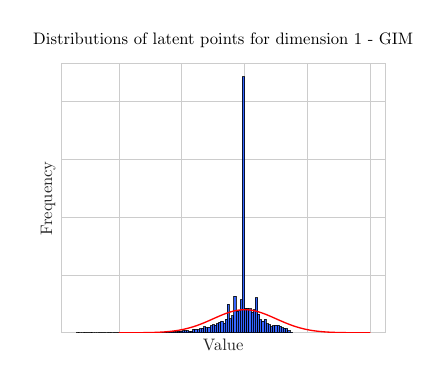
\begin{tikzpicture}[scale=0.6]

\definecolor{blue262255}{RGB}{2,62,255}
\definecolor{darkslategray38}{RGB}{38,38,38}
\definecolor{lightgray204}{RGB}{204,204,204}

\begin{axis}[
axis line style={lightgray204},
tick align=outside,
title={Distributions of latent points for dimension 1 - GIM},
x grid style={lightgray204},
xlabel=\textcolor{darkslategray38}{Value},
xmajorgrids,
xmajorticks=false,
xmin=-5.8340428352356, xmax=4.46828775405884,
xtick style={color=darkslategray38},
y grid style={lightgray204},
ylabel=\textcolor{darkslategray38}{Frequency},
ymajorgrids,
ymajorticks=false,
ymin=0, ymax=4.64754102146336,
ytick style={color=darkslategray38}
]
\draw[draw=black,fill=blue262255,opacity=0.8,line width=0.48pt] (axis cs:-5.36575508117676,0) rectangle (axis cs:-5.29699230194092,0.00193284839737247);
\draw[draw=black,fill=blue262255,opacity=0.8,line width=0.48pt] (axis cs:-5.29699230194092,0) rectangle (axis cs:-5.22822952270508,0);
\draw[draw=black,fill=blue262255,opacity=0.8,line width=0.48pt] (axis cs:-5.22822952270508,0) rectangle (axis cs:-5.1594672203064,0);
\draw[draw=black,fill=blue262255,opacity=0.8,line width=0.48pt] (axis cs:-5.1594672203064,0) rectangle (axis cs:-5.09070444107056,0);
\draw[draw=black,fill=blue262255,opacity=0.8,line width=0.48pt] (axis cs:-5.09070444107056,0) rectangle (axis cs:-5.02194166183472,0.00193284839737247);
\draw[draw=black,fill=blue262255,opacity=0.8,line width=0.48pt] (axis cs:-5.02194166183472,0) rectangle (axis cs:-4.95317888259888,0);
\draw[draw=black,fill=blue262255,opacity=0.8,line width=0.48pt] (axis cs:-4.95317840576172,0) rectangle (axis cs:-4.88441610336304,0.00193286180084944);
\draw[draw=black,fill=blue262255,opacity=0.8,line width=0.48pt] (axis cs:-4.8844165802002,0) rectangle (axis cs:-4.81565380096436,0);
\draw[draw=black,fill=blue262255,opacity=0.8,line width=0.48pt] (axis cs:-4.81565380096436,0) rectangle (axis cs:-4.74689102172852,0);
\draw[draw=black,fill=blue262255,opacity=0.8,line width=0.48pt] (axis cs:-4.74689102172852,0) rectangle (axis cs:-4.67812824249268,0);
\draw[draw=black,fill=blue262255,opacity=0.8,line width=0.48pt] (axis cs:-4.67812824249268,0) rectangle (axis cs:-4.60936546325684,0);
\draw[draw=black,fill=blue262255,opacity=0.8,line width=0.48pt] (axis cs:-4.60936546325684,0) rectangle (axis cs:-4.54060316085815,0);
\draw[draw=black,fill=blue262255,opacity=0.8,line width=0.48pt] (axis cs:-4.54060316085815,0) rectangle (axis cs:-4.47184038162231,0);
\draw[draw=black,fill=blue262255,opacity=0.8,line width=0.48pt] (axis cs:-4.47184038162231,0) rectangle (axis cs:-4.40307760238647,0);
\draw[draw=black,fill=blue262255,opacity=0.8,line width=0.48pt] (axis cs:-4.40307760238647,0) rectangle (axis cs:-4.33431482315063,0);
\draw[draw=black,fill=blue262255,opacity=0.8,line width=0.48pt] (axis cs:-4.33431482315063,0) rectangle (axis cs:-4.26555204391479,0.00386569679474493);
\draw[draw=black,fill=blue262255,opacity=0.8,line width=0.48pt] (axis cs:-4.26555156707764,0) rectangle (axis cs:-4.19678926467896,0);
\draw[draw=black,fill=blue262255,opacity=0.8,line width=0.48pt] (axis cs:-4.19678974151611,0) rectangle (axis cs:-4.12802696228027,0);
\draw[draw=black,fill=blue262255,opacity=0.8,line width=0.48pt] (axis cs:-4.12802696228027,0) rectangle (axis cs:-4.05926418304443,0);
\draw[draw=black,fill=blue262255,opacity=0.8,line width=0.48pt] (axis cs:-4.05926418304443,0) rectangle (axis cs:-3.99050188064575,0.00193285509908772);
\draw[draw=black,fill=blue262255,opacity=0.8,line width=0.48pt] (axis cs:-3.99050164222717,0) rectangle (axis cs:-3.92173886299133,0.00193284839737247);
\draw[draw=black,fill=blue262255,opacity=0.8,line width=0.48pt] (axis cs:-3.92173886299133,0) rectangle (axis cs:-3.85297656059265,0.00193285509908772);
\draw[draw=black,fill=blue262255,opacity=0.8,line width=0.48pt] (axis cs:-3.85297632217407,0) rectangle (axis cs:-3.78421354293823,0.00193284839737247);
\draw[draw=black,fill=blue262255,opacity=0.8,line width=0.48pt] (axis cs:-3.78421354293823,0) rectangle (axis cs:-3.71545076370239,0.00193284839737247);
\draw[draw=black,fill=blue262255,opacity=0.8,line width=0.48pt] (axis cs:-3.71545052528381,0) rectangle (axis cs:-3.64668822288513,0.00193285509908772);
\draw[draw=black,fill=blue262255,opacity=0.8,line width=0.48pt] (axis cs:-3.64668822288513,0) rectangle (axis cs:-3.57792544364929,0.00386569679474493);
\draw[draw=black,fill=blue262255,opacity=0.8,line width=0.48pt] (axis cs:-3.57792544364929,0) rectangle (axis cs:-3.50916314125061,0.00386571019817544);
\draw[draw=black,fill=blue262255,opacity=0.8,line width=0.48pt] (axis cs:-3.50916290283203,0) rectangle (axis cs:-3.44040012359619,0.00193284839737247);
\draw[draw=black,fill=blue262255,opacity=0.8,line width=0.48pt] (axis cs:-3.44039988517761,0) rectangle (axis cs:-3.37163758277893,0.00386571019817544);
\draw[draw=black,fill=blue262255,opacity=0.8,line width=0.48pt] (axis cs:-3.37163758277893,0) rectangle (axis cs:-3.30287480354309,0);
\draw[draw=black,fill=blue262255,opacity=0.8,line width=0.48pt] (axis cs:-3.30287480354309,0) rectangle (axis cs:-3.23411202430725,0.00193284839737247);
\draw[draw=black,fill=blue262255,opacity=0.8,line width=0.48pt] (axis cs:-3.23411202430725,0) rectangle (axis cs:-3.16534972190857,0.00193285509908772);
\draw[draw=black,fill=blue262255,opacity=0.8,line width=0.48pt] (axis cs:-3.16534948348999,0) rectangle (axis cs:-3.09658670425415,0.00386569679474493);
\draw[draw=black,fill=blue262255,opacity=0.8,line width=0.48pt] (axis cs:-3.09658646583557,0) rectangle (axis cs:-3.02782416343689,0.00579856529726315);
\draw[draw=black,fill=blue262255,opacity=0.8,line width=0.48pt] (axis cs:-3.02782416343689,0) rectangle (axis cs:-2.95906138420105,0.00193284839737247);
\draw[draw=black,fill=blue262255,opacity=0.8,line width=0.48pt] (axis cs:-2.95906138420105,0) rectangle (axis cs:-2.89029908180237,0);
\draw[draw=black,fill=blue262255,opacity=0.8,line width=0.48pt] (axis cs:-2.89029884338379,0) rectangle (axis cs:-2.82153606414795,0.00193284839737247);
\draw[draw=black,fill=blue262255,opacity=0.8,line width=0.48pt] (axis cs:-2.82153582572937,0) rectangle (axis cs:-2.75277352333069,0.00386571019817544);
\draw[draw=black,fill=blue262255,opacity=0.8,line width=0.48pt] (axis cs:-2.75277352333069,0) rectangle (axis cs:-2.68401074409485,0.0115970903842348);
\draw[draw=black,fill=blue262255,opacity=0.8,line width=0.48pt] (axis cs:-2.68401074409485,0) rectangle (axis cs:-2.61524796485901,0.00773139358948987);
\draw[draw=black,fill=blue262255,opacity=0.8,line width=0.48pt] (axis cs:-2.61524796485901,0) rectangle (axis cs:-2.54648566246033,0.00579856529726315);
\draw[draw=black,fill=blue262255,opacity=0.8,line width=0.48pt] (axis cs:-2.54648542404175,0) rectangle (axis cs:-2.47772264480591,0.00773139358948987);
\draw[draw=black,fill=blue262255,opacity=0.8,line width=0.48pt] (axis cs:-2.47772240638733,0) rectangle (axis cs:-2.40896010398865,0.0154628407927017);
\draw[draw=black,fill=blue262255,opacity=0.8,line width=0.48pt] (axis cs:-2.40896010398865,0) rectangle (axis cs:-2.34019732475281,0.0193284839737247);
\draw[draw=black,fill=blue262255,opacity=0.8,line width=0.48pt] (axis cs:-2.34019732475281,0) rectangle (axis cs:-2.27143502235413,0.0212614060899649);
\draw[draw=black,fill=blue262255,opacity=0.8,line width=0.48pt] (axis cs:-2.27143478393555,0) rectangle (axis cs:-2.20267200469971,0.0173956355763522);
\draw[draw=black,fill=blue262255,opacity=0.8,line width=0.48pt] (axis cs:-2.20267200469971,0) rectangle (axis cs:-2.13390922546387,0.0154627871789797);
\draw[draw=black,fill=blue262255,opacity=0.8,line width=0.48pt] (axis cs:-2.13390898704529,0) rectangle (axis cs:-2.06514668464661,0.027059971387228);
\draw[draw=black,fill=blue262255,opacity=0.8,line width=0.48pt] (axis cs:-2.06514668464661,0) rectangle (axis cs:-1.99638390541077,0.0309256279715885);
\draw[draw=black,fill=blue262255,opacity=0.8,line width=0.48pt] (axis cs:-1.99638414382935,0) rectangle (axis cs:-1.92762136459351,0.0367241832162614);
\draw[draw=black,fill=blue262255,opacity=0.8,line width=0.48pt] (axis cs:-1.92762136459351,0) rectangle (axis cs:-1.85885858535767,0.0347912711527044);
\draw[draw=black,fill=blue262255,opacity=0.8,line width=0.48pt] (axis cs:-1.85885858535767,0) rectangle (axis cs:-1.79009580612183,0.0347913314680371);
\draw[draw=black,fill=blue262255,opacity=0.8,line width=0.48pt] (axis cs:-1.79009604454041,0) rectangle (axis cs:-1.72133326530457,0.0231942209786914);
\draw[draw=black,fill=blue262255,opacity=0.8,line width=0.48pt] (axis cs:-1.72133326530457,0) rectangle (axis cs:-1.65257048606873,0.0289927762233642);
\draw[draw=black,fill=blue262255,opacity=0.8,line width=0.48pt] (axis cs:-1.6525707244873,0) rectangle (axis cs:-1.58380794525146,0.0579855524467285);
\draw[draw=black,fill=blue262255,opacity=0.8,line width=0.48pt] (axis cs:-1.58380794525146,0) rectangle (axis cs:-1.51504516601562,0.0657169594396256);
\draw[draw=black,fill=blue262255,opacity=0.8,line width=0.48pt] (axis cs:-1.5150454044342,0) rectangle (axis cs:-1.44628262519836,0.0560527006985042);
\draw[draw=black,fill=blue262255,opacity=0.8,line width=0.48pt] (axis cs:-1.44628262519836,0) rectangle (axis cs:-1.37751984596252,0.0676496939080363);
\draw[draw=black,fill=blue262255,opacity=0.8,line width=0.48pt] (axis cs:-1.37751984596252,0) rectangle (axis cs:-1.30875706672668,0.0773140699289713);
\draw[draw=black,fill=blue262255,opacity=0.8,line width=0.48pt] (axis cs:-1.30875730514526,0) rectangle (axis cs:-1.23999452590942,0.102441142655887);
\draw[draw=black,fill=blue262255,opacity=0.8,line width=0.48pt] (axis cs:-1.23999452590942,0) rectangle (axis cs:-1.17123174667358,0.088911180418317);
\draw[draw=black,fill=blue262255,opacity=0.8,line width=0.48pt] (axis cs:-1.17123198509216,0) rectangle (axis cs:-1.10246920585632,0.0966425874112141);
\draw[draw=black,fill=blue262255,opacity=0.8,line width=0.48pt] (axis cs:-1.10246920585632,0) rectangle (axis cs:-1.03370642662048,0.123702511886354);
\draw[draw=black,fill=blue262255,opacity=0.8,line width=0.48pt] (axis cs:-1.03370654582977,0) rectangle (axis cs:-0.964943766593933,0.141098055314175);
\draw[draw=black,fill=blue262255,opacity=0.8,line width=0.48pt] (axis cs:-0.964943885803223,0) rectangle (axis cs:-0.896181106567383,0.131433918879251);
\draw[draw=black,fill=blue262255,opacity=0.8,line width=0.48pt] (axis cs:-0.896181225776672,0) rectangle (axis cs:-0.827418446540833,0.154628139857943);
\draw[draw=black,fill=blue262255,opacity=0.8,line width=0.48pt] (axis cs:-0.827418565750122,0) rectangle (axis cs:-0.758655786514282,0.187486619577755);
\draw[draw=black,fill=blue262255,opacity=0.8,line width=0.48pt] (axis cs:-0.758655905723572,0) rectangle (axis cs:-0.689893126487732,0.199083557498083);
\draw[draw=black,fill=blue262255,opacity=0.8,line width=0.48pt] (axis cs:-0.689893186092377,0) rectangle (axis cs:-0.621130406856537,0.164292398599064);
\draw[draw=black,fill=blue262255,opacity=0.8,line width=0.48pt] (axis cs:-0.621130526065826,0) rectangle (axis cs:-0.552367746829987,0.231942209786914);
\draw[draw=black,fill=blue262255,opacity=0.8,line width=0.48pt] (axis cs:-0.552367866039276,0) rectangle (axis cs:-0.483605086803436,0.489011280359091);
\draw[draw=black,fill=blue262255,opacity=0.8,line width=0.48pt] (axis cs:-0.483605176210403,0) rectangle (axis cs:-0.414842396974564,0.24353932027626);
\draw[draw=black,fill=blue262255,opacity=0.8,line width=0.48pt] (axis cs:-0.414842486381531,0) rectangle (axis cs:-0.346079707145691,0.295726189308067);
\draw[draw=black,fill=blue262255,opacity=0.8,line width=0.48pt] (axis cs:-0.34607982635498,0) rectangle (axis cs:-0.277317047119141,0.635908225165789);
\draw[draw=black,fill=blue262255,opacity=0.8,line width=0.48pt] (axis cs:-0.27731716632843,0) rectangle (axis cs:-0.20855438709259,0.373040225728476);
\draw[draw=black,fill=blue262255,opacity=0.8,line width=0.48pt] (axis cs:-0.208554476499557,0) rectangle (axis cs:-0.139791697263718,0.392368819861536);
\draw[draw=black,fill=blue262255,opacity=0.8,line width=0.48pt] (axis cs:-0.139791786670685,0) rectangle (axis cs:-0.071029007434845,0.570191142163315);
\draw[draw=black,fill=blue262255,opacity=0.8,line width=0.48pt] (axis cs:-0.0710291191935539,0) rectangle (axis cs:-0.00226633995771408,4.42622954425082);
\draw[draw=black,fill=blue262255,opacity=0.8,line width=0.48pt] (axis cs:-0.00226644426584244,0) rectangle (axis cs:0.0664963349699974,0.425227292460778);
\draw[draw=black,fill=blue262255,opacity=0.8,line width=0.48pt] (axis cs:0.066496230661869,0) rectangle (axis cs:0.135259002447128,0.42329444113141);
\draw[draw=black,fill=blue262255,opacity=0.8,line width=0.48pt] (axis cs:0.135258913040161,0) rectangle (axis cs:0.204021692276001,0.419428738472676);
\draw[draw=black,fill=blue262255,opacity=0.8,line width=0.48pt] (axis cs:0.204021587967873,0) rectangle (axis cs:0.272784352302551,0.351778865712864);
\draw[draw=black,fill=blue262255,opacity=0.8,line width=0.48pt] (axis cs:0.272784262895584,0) rectangle (axis cs:0.341547042131424,0.402033163630651);
\draw[draw=black,fill=blue262255,opacity=0.8,line width=0.48pt] (axis cs:0.341546952724457,0) rectangle (axis cs:0.410309731960297,0.606915185900215);
\draw[draw=black,fill=blue262255,opacity=0.8,line width=0.48pt] (axis cs:0.410309612751007,0) rectangle (axis cs:0.479072391986847,0.320853390205231);
\draw[draw=black,fill=blue262255,opacity=0.8,line width=0.48pt] (axis cs:0.479072272777557,0) rectangle (axis cs:0.547835052013397,0.226143654542241);
\draw[draw=black,fill=blue262255,opacity=0.8,line width=0.48pt] (axis cs:0.547834992408752,0) rectangle (axis cs:0.616597771644592,0.20101640757088);
\draw[draw=black,fill=blue262255,opacity=0.8,line width=0.48pt] (axis cs:0.616597652435303,0) rectangle (axis cs:0.685360431671143,0.231942209786914);
\draw[draw=black,fill=blue262255,opacity=0.8,line width=0.48pt] (axis cs:0.685360312461853,0) rectangle (axis cs:0.754123091697693,0.160426695102615);
\draw[draw=black,fill=blue262255,opacity=0.8,line width=0.48pt] (axis cs:0.754122972488403,0) rectangle (axis cs:0.822885751724243,0.137232474123924);
\draw[draw=black,fill=blue262255,opacity=0.8,line width=0.48pt] (axis cs:0.822885632514954,0) rectangle (axis cs:0.891648411750793,0.102441053858237);
\draw[draw=black,fill=blue262255,opacity=0.8,line width=0.48pt] (axis cs:0.891648352146149,0) rectangle (axis cs:0.960411131381989,0.123702511886354);
\draw[draw=black,fill=blue262255,opacity=0.8,line width=0.48pt] (axis cs:0.960411012172699,0) rectangle (axis cs:1.02917385101318,0.129501067131027);
\draw[draw=black,fill=blue262255,opacity=0.8,line width=0.48pt] (axis cs:1.0291736125946,0) rectangle (axis cs:1.09793639183044,0.127568215382803);
\draw[draw=black,fill=blue262255,opacity=0.8,line width=0.48pt] (axis cs:1.09793639183044,0) rectangle (axis cs:1.16669917106628,0.110172549648784);
\draw[draw=black,fill=blue262255,opacity=0.8,line width=0.48pt] (axis cs:1.16669893264771,0) rectangle (axis cs:1.23546171188354,0.0908440321665413);
\draw[draw=black,fill=blue262255,opacity=0.8,line width=0.48pt] (axis cs:1.23546171188354,0) rectangle (axis cs:1.30422449111938,0.0773139358948986);
\draw[draw=black,fill=blue262255,opacity=0.8,line width=0.48pt] (axis cs:1.30422449111938,0) rectangle (axis cs:1.37298727035522,0.0676498111878499);
\draw[draw=black,fill=blue262255,opacity=0.8,line width=0.48pt] (axis cs:1.37298703193665,0) rectangle (axis cs:1.44174981117249,0.0328584797198128);
\draw[draw=black,fill=blue262255,opacity=0.8,line width=0.48pt] (axis cs:1.44174981117249,0) rectangle (axis cs:1.51051259040833,0.00773140699289713);
\addplot [thick, red]
table {%
-4 0.000133830225764885
-3.99199199199199 0.000138182046410498
-3.98398398398398 0.000142666228042307
-3.97597597597598 0.000147286481503254
-3.96796796796797 0.000152046611333821
-3.95995995995996 0.000156950517814782
-3.95195195195195 0.00016200219904485
-3.94394394394394 0.00016720575305353
-3.93593593593594 0.000172565379949496
-3.92792792792793 0.00017808538410479
-3.91991991991992 0.000183770176375138
-3.91191191191191 0.000189624276356684
-3.9039039039039 0.000195652314679408
-3.8958958958959 0.000201859035337517
-3.88788788788789 0.000208249298057069
-3.87987987987988 0.000214828080701088
-3.87187187187187 0.000221600481712426
-3.86386386386386 0.0002285717225946
-3.85585585585586 0.000235747150430845
-3.84784784784785 0.000243132240441603
-3.83983983983984 0.000250732598580649
-3.83183183183183 0.000258553964170059
-3.82382382382382 0.000266602212574213
-3.81581581581582 0.000274883357912987
-3.80780780780781 0.000283403555814325
-3.7997997997998 0.000292169106206322
-3.79179179179179 0.000301186456148957
-3.78378378378378 0.0003104622027056
-3.77577577577578 0.000320003095854415
-3.76776776776777 0.000329816041439723
-3.75975975975976 0.000339908104163431
-3.75175175175175 0.00035028651061658
-3.74374374374374 0.000360958652351047
-3.73573573573574 0.000371932088991451
-3.72772772772773 0.000383214551387261
-3.71971971971972 0.000394813944805093
-3.71171171171171 0.000406738352161197
-3.7037037037037 0.000418996037294058
-3.6956956956957 0.00043159544827708
-3.68768768768769 0.00044454522077123
-3.67967967967968 0.000457854181417586
-3.67167167167167 0.000471531351269624
-3.66366366366366 0.000485585949265103
-3.65565565565566 0.000500027395737409
-3.64764764764765 0.000514865315966112
-3.63963963963964 0.000530109543766577
-3.63163163163163 0.000545770125118336
-3.62362362362362 0.000561857321831991
-3.61561561561562 0.00057838161525435
-3.60760760760761 0.000595353710011453
-3.5995995995996 0.000612784537789192
-3.59159159159159 0.000630685261151105
-3.58358358358358 0.000649067277392973
-3.57557557557558 0.000667942222433796
-3.56756756756757 0.000687321974742665
-3.55955955955956 0.000707218659301081
-3.55155155155155 0.000727644651600166
-3.54354354354354 0.000748612581672245
-3.53553553553554 0.000770135338156225
-3.52752752752753 0.000792226072396121
-3.51951951951952 0.00081489820257214
-3.51151151151151 0.000838165417863603
-3.5035035035035 0.000862041682643007
-3.4954954954955 0.000886541240700502
-3.48748748748749 0.00091167861949796
-3.47947947947948 0.000937468634451866
-3.47147147147147 0.000963926393244149
-3.46346346346346 0.000991067300160059
-3.45545545545546 0.0010189070604522
-3.44744744744745 0.00104746168472971
-3.43943943943944 0.0010767474933716
-3.43143143143143 0.00110678112096323
-3.42342342342342 0.00113757952075483
-3.41541541541542 0.00116915996914087
-3.40740740740741 0.00120154007015926
-3.3993993993994 0.00123473776000907
-3.39139139139139 0.00126877131158549
-3.38338338338338 0.00130365933903088
-3.37537537537538 0.00133942080230046
-3.36736736736737 0.00137607501174126
-3.35935935935936 0.001413641632683
-3.35135135135135 0.00145214069003938
-3.34334334334334 0.0014915925729182
-3.33533533533534 0.00153201803923895
-3.32732732732733 0.00157343822035606
-3.31931931931932 0.00161587462568624
-3.31131131131131 0.00165934914733831
-3.3033033033033 0.00170388406474362
-3.2952952952953 0.00174950204928538
-3.28728728728729 0.00179622616892505
-3.27927927927928 0.00184407989282385
-3.27127127127127 0.00189308709595757
-3.26326326326326 0.00194327206372255
-3.25525525525526 0.00199465949653091
-3.24724724724725 0.00204727451439301
-3.23923923923924 0.00210114266148476
-3.23123123123123 0.00215628991069791
-3.22322322322322 0.00221274266817093
-3.21521521521522 0.00227052777779815
-3.20720720720721 0.00232967252571501
-3.1991991991992 0.00239020464475689
-3.19119119119119 0.00245215231888918
-3.18318318318318 0.00251554418760605
-3.17517517517518 0.00258040935029545
-3.16716716716717 0.00264677737056774
-3.15915915915916 0.00271467828054534
-3.15115115115115 0.00278414258511061
-3.14314314314314 0.00285520126610952
-3.13513513513514 0.00292788578650791
-3.12712712712713 0.00300222809449793
-3.11911911911912 0.00307826062755151
-3.11111111111111 0.00315601631641804
-3.1031031031031 0.00323552858906328
-3.0950950950951 0.00331683137454643
-3.08708708708709 0.00339995910683238
-3.07907907907908 0.00348494672853595
-3.07107107107107 0.00357182969459489
-3.06306306306306 0.00366064397586864
-3.05505505505506 0.00375142606265932
-3.04704704704705 0.00384421296815189
-3.03903903903904 0.00393904223176991
-3.03103103103103 0.00403595192244368
-3.02302302302302 0.0041349806417872
-3.01501501501502 0.00423616752718052
-3.00700700700701 0.00433955225475399
-2.998998998999 0.00444517504227068
-2.99099099099099 0.00455307665190355
-2.98298298298298 0.00466329839290368
-2.97497497497497 0.00477588212415564
-2.96696696696697 0.00489087025661667
-2.95895895895896 0.00500830575563558
-2.95095095095095 0.00512823214314763
-2.94294294294294 0.00525069349974172
-2.93493493493493 0.00537573446659573
-2.92692692692693 0.00550340024727644
-2.91891891891892 0.00563373660939975
-2.91091091091091 0.0057667898861475
-2.9029029029029 0.00590260697763674
-2.89489489489489 0.00604123535213746
-2.88688688688689 0.00618272304713484
-2.87887887887888 0.00632711867023164
-2.87087087087087 0.00647447139988703
-2.86286286286286 0.00662483098598741
-2.85485485485485 0.0067782477502453
-2.84684684684685 0.0069347725864219
-2.83883883883884 0.00709445696036946
-2.83083083083083 0.00725735290988893
-2.82282282282282 0.00742351304439893
-2.81481481481481 0.00759299054441176
-2.80680680680681 0.0077658391608121
-2.7987987987988 0.00794211321393437
-2.79079079079079 0.00812186759243432
-2.78278278278278 0.00830515775195071
-2.77477477477477 0.00849203971355293
-2.76676676676677 0.00868257006197001
-2.75875875875876 0.00887680594359712
-2.75075075075075 0.00907480506427511
-2.74274274274274 0.00927662568683898
-2.73473473473473 0.00948232662843099
-2.72672672672673 0.00969196725757422
-2.71871871871872 0.00990560749100246
-2.71071071071071 0.0101233077902421
-2.7027027027027 0.0103451291579421
-2.69469469469469 0.0105711331339476
-2.68668668668669 0.0108013817911136
-2.67867867867868 0.011035937730854
-2.67067067067067 0.0112748640784219
-2.66266266266266 0.0115182244779185
-2.65465465465465 0.0117660830870247
-2.64664664664665 0.0120185045714526
-2.63863863863864 0.0122755540991133
-2.63063063063063 0.0125372973339956
-2.62262262262262 0.0128038004297541
-2.61461461461461 0.0130751300230007
-2.60660660660661 0.0133513532262973
-2.5985985985986 0.0136325376208454
-2.59059059059059 0.0139187512488692
-2.58258258258258 0.014210062605689
-2.57457457457457 0.0145065406314803
-2.56656656656657 0.0148082547027168
-2.55855855855856 0.0151152746232934
-2.55055055055055 0.0154276706153247
-2.54254254254254 0.0157455133096184
-2.53453453453453 0.0160688737358178
-2.52652652652653 0.016397823312213
-2.51851851851852 0.0167324338352151
-2.51051051051051 0.0170727774684938
-2.5025025025025 0.0174189267317727
-2.49449449449449 0.0177709544892815
-2.48648648648649 0.0181289339378627
-2.47847847847848 0.0184929385947284
-2.47047047047047 0.0188630422848682
-2.46246246246246 0.0192393191281025
-2.45445445445445 0.0196218435257817
-2.44644644644645 0.0200106901471285
-2.43843843843844 0.020405933915221
-2.43043043043043 0.0208076499926159
-2.42242242242242 0.0212159137666093
-2.41441441441441 0.0216308008341344
-2.40640640640641 0.0220523869862944
-2.3983983983984 0.0224807481925294
-2.39039039039039 0.022915960584417
-2.38238238238238 0.0233581004391047
-2.37437437437437 0.023807244162374
-2.36636636636637 0.0242634682713357
-2.35835835835836 0.0247268493767558
-2.35035035035035 0.0251974641650118
-2.34234234234234 0.0256753893796796
-2.33433433433433 0.0261607018027501
-2.32632632632633 0.0266534782354775
-2.31831831831832 0.0271537954788581
-2.31031031031031 0.0276617303137407
-2.3023023023023 0.0281773594805703
-2.29429429429429 0.0287007596587648
-2.28628628628629 0.0292320074457259
-2.27827827827828 0.029771179335487
-2.27027027027027 0.0303183516969979
-2.26226226226226 0.0308736007520491
-2.25425425425425 0.0314370025528369
-2.24624624624625 0.0320086329591723
-2.23823823823824 0.0325885676153351
-2.23023023023023 0.0331768819265761
-2.22222222222222 0.0337736510352706
-2.21421421421421 0.0343789497967251
-2.20620620620621 0.0349928527546413
-2.1981981981982 0.0356154341162401
-2.19019019019019 0.0362467677270497
-2.18218218218218 0.0368869270453615
-2.17417417417417 0.0375359851163567
-2.16616616616617 0.03819401454591
-2.15815815815816 0.0388610874740724
-2.15015015015015 0.03953727554824
-2.14214214214214 0.0402226498960119
-2.13413413413413 0.0409172810977437
-2.12612612612613 0.0416212391588003
-2.11811811811812 0.0423345934815158
-2.11011011011011 0.0430574128368641
-2.1021021021021 0.043789765335848
-2.09409409409409 0.0445317184006117
-2.08608608608609 0.0452833387352837
-2.07807807807808 0.0460446922965577
-2.07007007007007 0.0468158442640166
-2.06206206206206 0.0475968590102091
-2.05405405405405 0.0483878000704834
-2.04604604604605 0.0491887301125894
-2.03803803803804 0.0499997109060533
-2.03003003003003 0.0508208032913361
-2.02202202202202 0.0516520671487823
-2.01401401401401 0.0524935613673682
-2.00600600600601 0.053345343813258
-1.997997997998 0.0542074712981785
-1.98998998998999 0.0550799995476186
-1.98198198198198 0.0559629831688668
-1.97397397397397 0.0568564756188931
-1.96596596596597 0.0577605291720876
-1.95795795795796 0.0586751948878651
-1.94994994994995 0.0596005225781457
-1.94194194194194 0.0605365607747232
-1.93393393393393 0.0614833566965309
-1.92592592592593 0.062440956216817
-1.91791791791792 0.06340940383024
-1.90990990990991 0.0643887426198963
-1.9019019019019 0.0653790142242912
-1.89389389389389 0.0663802588042656
-1.88588588588589 0.0673925150098903
-1.87787787787788 0.0684158199473405
-1.86986986986987 0.0694502091457625
-1.86186186186186 0.0704957165241465
-1.85385385385385 0.0715523743582165
-1.84584584584585 0.0726202132473521
-1.83783783783784 0.0736992620815557
-1.82982982982983 0.0747895480084762
-1.82182182182182 0.0758910964005057
-1.81381381381381 0.0770039308219614
-1.80580580580581 0.0781280729963669
-1.7977977977978 0.0792635427738473
-1.78978978978979 0.0804103580986525
-1.78178178178178 0.0815685349768227
-1.77377377377377 0.0827380874440109
-1.76576576576577 0.0839190275334777
-1.75775775775776 0.0851113652442723
-1.74974974974975 0.086315108509615
-1.74174174174174 0.0875302631654975
-1.73373373373373 0.0887568329195139
-1.72572572572573 0.0899948193199405
-1.71771771771772 0.0912442217250772
-1.70970970970971 0.0925050372728685
-1.7017017017017 0.0937772608508177
-1.69369369369369 0.0950608850662112
-1.68568568568569 0.0963559002166691
-1.67767767767768 0.0976622942610365
-1.66966966966967 0.0989800527906321
-1.66166166166166 0.100309159000872
-1.65365365365365 0.10164959366328
-1.64564564564565 0.103001335097907
-1.63763763763764 0.10436435914617
-1.62962962962963 0.105738639144131
-1.62162162162162 0.107124145896225
-1.61361361361361 0.108520847649465
-1.60560560560561 0.10992871006813
-1.5975975975976 0.111347696208955
-1.58958958958959 0.112777766496842
-1.58158158158158 0.114218878701105
-1.57357357357357 0.115670987912262
-1.56556556556557 0.117134046519405
-1.55755755755756 0.11860800418814
-1.54954954954955 0.120092807839133
-1.54154154154154 0.121588401627275
-1.53353353353353 0.123094726921466
-1.52552552552553 0.124611722285057
-1.51751751751752 0.12613932345695
-1.50950950950951 0.127677463333369
-1.5015015015015 0.129226071950339
-1.49349349349349 0.130785076466857
-1.48548548548549 0.132354401148798
-1.47747747747748 0.133933967353555
-1.46946946946947 0.13552369351543
-1.46146146146146 0.137123495131801
-1.45345345345345 0.13873328475006
-1.44544544544545 0.140352971955359
-1.43743743743744 0.141982463359159
-1.42942942942943 0.143621662588612
-1.42142142142142 0.14527047027677
-1.41341341341341 0.146928784053658
-1.40540540540541 0.148596498538208
-1.3973973973974 0.150273505331067
-1.38938938938939 0.151959693008306
-1.38138138138138 0.153654947116025
-1.37337337337337 0.155359150165875
-1.36536536536537 0.157072181631514
-1.35735735735736 0.158793917945997
-1.34934934934935 0.160524232500121
-1.34134134134134 0.16226299564173
-1.33333333333333 0.164010074675994
-1.32532532532533 0.165765333866673
-1.31731731731732 0.167528634438376
-1.30930930930931 0.169299834579821
-1.3013013013013 0.17107878944811
-1.29329329329329 0.172865351174024
-1.28528528528529 0.174659368868355
-1.27727727727728 0.176460688629273
-1.26926926926927 0.178269153550739
-1.26126126126126 0.180084603731981
-1.25325325325325 0.181906876288021
-1.24524524524525 0.183735805361283
-1.23723723723724 0.185571222134271
-1.22922922922923 0.187412954843324
-1.22122122122122 0.18926082879347
-1.21321321321321 0.191114666374361
-1.20520520520521 0.192974287077311
-1.1971971971972 0.194839507513435
-1.18918918918919 0.19671014143289
-1.18118118118118 0.198585999745227
-1.17317317317317 0.200466890540856
-1.16516516516517 0.202352619113618
-1.15715715715716 0.204242987984477
-1.14914914914915 0.206137796926331
-1.14114114114114 0.208036842989938
-1.13313313313313 0.209939920530956
-1.12512512512513 0.21184682123811
-1.11711711711712 0.21375733416247
-1.10910910910911 0.215671245747847
-1.1011011011011 0.217588339862305
-1.09309309309309 0.219508397830784
-1.08508508508509 0.221431198468836
-1.07707707707708 0.223356518117463
-1.06906906906907 0.225284130679063
-1.06106106106106 0.22721380765447
-1.05305305305305 0.229145318181096
-1.04504504504505 0.231078429072154
-1.03703703703704 0.233012904856966
-1.02902902902903 0.234948507822352
-1.02102102102102 0.236884998055083
-1.01301301301301 0.238822133485401
-1.00500500500501 0.24075966993159
-0.996996996996997 0.242697361145593
-0.988988988988989 0.244634958859672
-0.980980980980981 0.246572212834085
-0.972972972972973 0.248508870905785
-0.964964964964965 0.250444679038131
-0.956956956956957 0.252379381371581
-0.948948948948949 0.254312720275385
-0.940940940940941 0.256244436400228
-0.932932932932933 0.258174268731856
-0.924924924924925 0.260101954645624
-0.916916916916917 0.262027229961987
-0.908908908908909 0.263949829002911
-0.900900900900901 0.265869484649172
-0.892892892892893 0.267785928398552
-0.884884884884885 0.269698890424904
-0.876876876876877 0.271608099638066
-0.868868868868869 0.273513283744617
-0.860860860860861 0.275414169309444
-0.852852852852853 0.277310481818125
-0.844844844844845 0.279201945740075
-0.836836836836837 0.281088284592474
-0.828828828828829 0.28296922100493
-0.820820820820821 0.284844476784867
-0.812812812812813 0.286713772983616
-0.804804804804805 0.288576829963198
-0.796796796796797 0.290433367463758
-0.788788788788789 0.292283104671645
-0.780780780780781 0.294125760288111
-0.772772772772773 0.295961052598604
-0.764764764764765 0.29778869954263
-0.756756756756757 0.299608418784177
-0.748748748748749 0.301419927782648
-0.740740740740741 0.303222943864308
-0.732732732732733 0.305017184294205
-0.724724724724725 0.306802366348536
-0.716716716716717 0.308578207387456
-0.708708708708709 0.310344424928268
-0.700700700700701 0.312100736719007
-0.692692692692693 0.313846860812361
-0.684684684684685 0.31558251563992
-0.676676676676677 0.317307420086723
-0.668668668668669 0.319021293566066
-0.660660660660661 0.320723856094559
-0.652652652652653 0.322414828367396
-0.644644644644645 0.324093931833804
-0.636636636636636 0.325760888772662
-0.628628628628629 0.327415422368237
-0.620620620620621 0.329057256786028
-0.612612612612613 0.330686117248681
-0.604604604604605 0.33230173011195
-0.596596596596596 0.333903822940662
-0.588588588588589 0.335492124584683
-0.580580580580581 0.337066365254824
-0.572572572572573 0.338626276598684
-0.564564564564565 0.340171591776383
-0.556556556556556 0.341702045536168
-0.548548548548549 0.343217374289848
-0.54054054054054 0.344717316188045
-0.532532532532533 0.346201611195215
-0.524524524524525 0.347670001164422
-0.516516516516516 0.349122229911825
-0.508508508508509 0.350558043290856
-0.5005005005005 0.351977189266054
-0.492492492492492 0.353379417986526
-0.484484484484485 0.354764481859011
-0.476476476476476 0.356132135620502
-0.468468468468469 0.357482136410418
-0.46046046046046 0.358814243842273
-0.452452452452452 0.360128220074839
-0.444444444444445 0.361423829882744
-0.436436436436436 0.362700840726495
-0.428428428428429 0.363959022821904
-0.42042042042042 0.365198149208855
-0.412412412412412 0.366417995819425
-0.404404404404405 0.3676183415453
-0.396396396396396 0.368798968304465
-0.388388388388389 0.369959661107154
-0.38038038038038 0.37110020812101
-0.372372372372372 0.372220400735444
-0.364364364364365 0.373320033625156
-0.356356356356356 0.374398904812801
-0.348348348348348 0.375456815730761
-0.34034034034034 0.376493571282005
-0.332332332332332 0.377508979900006
-0.324324324324325 0.378502853607702
-0.316316316316316 0.379475008075448
-0.308308308308308 0.380425262677969
-0.3003003003003 0.38135344055026
-0.292292292292292 0.382259368642425
-0.284284284284285 0.38314287777343
-0.276276276276276 0.384003802683735
-0.268268268268268 0.3848419820868
-0.26026026026026 0.385657258719425
-0.252252252252252 0.386449479390916
-0.244244244244244 0.387218495031049
-0.236236236236236 0.387964160736805
-0.228228228228228 0.38868633581787
-0.22022022022022 0.389384883840873
-0.212212212212212 0.390059672672329
-0.204204204204204 0.390710574520297
-0.196196196196196 0.391337465974705
-0.188188188188188 0.39194022804635
-0.18018018018018 0.392518746204527
-0.172172172172172 0.393072910413305
-0.164164164164164 0.393602615166401
-0.156156156156156 0.394107759520658
-0.148148148148148 0.394588247128102
-0.14014014014014 0.395043986266573
-0.132132132132132 0.3954748898689
-0.124124124124124 0.395880875550626
-0.116116116116116 0.396261865636259
-0.108108108108108 0.396617787184037
-0.1001001001001 0.396948572009207
-0.0920920920920922 0.397254156705792
-0.084084084084084 0.397534482666846
-0.0760760760760761 0.39778949610319
-0.0680680680680683 0.39801914806061
-0.06006006006006 0.398223394435522
-0.0520520520520522 0.398402195989086
-0.0440440440440439 0.398555518359772
-0.0360360360360361 0.398683332074364
-0.0280280280280278 0.398785612557403
-0.02002002002002 0.398862340139061
-0.0120120120120122 0.398913500061449
-0.00400400400400391 0.398939082483343
0.00400400400400436 0.398939082483343
0.0120120120120122 0.398913500061449
0.02002002002002 0.398862340139061
0.0280280280280278 0.398785612557403
0.0360360360360357 0.398683332074364
0.0440440440440444 0.398555518359772
0.0520520520520522 0.398402195989086
0.06006006006006 0.398223394435522
0.0680680680680679 0.39801914806061
0.0760760760760757 0.39778949610319
0.0840840840840844 0.397534482666846
0.0920920920920922 0.397254156705792
0.1001001001001 0.396948572009207
0.108108108108108 0.396617787184037
0.116116116116116 0.396261865636259
0.124124124124124 0.395880875550626
0.132132132132132 0.3954748898689
0.14014014014014 0.395043986266573
0.148148148148148 0.394588247128102
0.156156156156156 0.394107759520658
0.164164164164164 0.393602615166401
0.172172172172172 0.393072910413305
0.18018018018018 0.392518746204527
0.188188188188188 0.39194022804635
0.196196196196196 0.391337465974705
0.204204204204204 0.390710574520297
0.212212212212212 0.390059672672329
0.22022022022022 0.389384883840873
0.228228228228228 0.388686335817871
0.236236236236236 0.387964160736805
0.244244244244245 0.387218495031049
0.252252252252252 0.386449479390916
0.26026026026026 0.385657258719425
0.268268268268268 0.3848419820868
0.276276276276276 0.384003802683735
0.284284284284285 0.38314287777343
0.292292292292292 0.382259368642425
0.3003003003003 0.38135344055026
0.308308308308308 0.380425262677969
0.316316316316316 0.379475008075448
0.324324324324325 0.378502853607702
0.332332332332332 0.377508979900006
0.34034034034034 0.376493571282005
0.348348348348348 0.375456815730762
0.356356356356356 0.374398904812801
0.364364364364365 0.373320033625156
0.372372372372372 0.372220400735444
0.38038038038038 0.37110020812101
0.388388388388388 0.369959661107154
0.396396396396397 0.368798968304465
0.404404404404405 0.3676183415453
0.412412412412412 0.366417995819425
0.42042042042042 0.365198149208855
0.428428428428428 0.363959022821904
0.436436436436437 0.362700840726495
0.444444444444445 0.361423829882744
0.452452452452452 0.360128220074839
0.46046046046046 0.358814243842273
0.468468468468468 0.357482136410418
0.476476476476477 0.356132135620502
0.484484484484485 0.354764481859011
0.492492492492492 0.353379417986526
0.5005005005005 0.351977189266054
0.508508508508508 0.350558043290856
0.516516516516517 0.349122229911825
0.524524524524525 0.347670001164422
0.532532532532533 0.346201611195215
0.54054054054054 0.344717316188045
0.548548548548548 0.343217374289848
0.556556556556557 0.341702045536168
0.564564564564565 0.340171591776383
0.572572572572573 0.338626276598684
0.58058058058058 0.337066365254824
0.588588588588588 0.335492124584683
0.596596596596597 0.333903822940662
0.604604604604605 0.33230173011195
0.612612612612613 0.330686117248681
0.62062062062062 0.329057256786028
0.628628628628628 0.327415422368237
0.636636636636637 0.325760888772662
0.644644644644645 0.324093931833804
0.652652652652653 0.322414828367396
0.66066066066066 0.32072385609456
0.668668668668668 0.319021293566066
0.676676676676677 0.317307420086723
0.684684684684685 0.31558251563992
0.692692692692693 0.313846860812361
0.7007007007007 0.312100736719007
0.708708708708708 0.310344424928268
0.716716716716717 0.308578207387456
0.724724724724725 0.306802366348536
0.732732732732733 0.305017184294205
0.74074074074074 0.303222943864308
0.748748748748748 0.301419927782648
0.756756756756757 0.299608418784177
0.764764764764765 0.29778869954263
0.772772772772773 0.295961052598604
0.780780780780781 0.294125760288111
0.788788788788788 0.292283104671645
0.796796796796797 0.290433367463758
0.804804804804805 0.288576829963198
0.812812812812813 0.286713772983616
0.820820820820821 0.284844476784867
0.828828828828828 0.282969221004931
0.836836836836837 0.281088284592474
0.844844844844845 0.279201945740075
0.852852852852853 0.277310481818125
0.860860860860861 0.275414169309444
0.868868868868869 0.273513283744617
0.876876876876877 0.271608099638066
0.884884884884885 0.269698890424904
0.892892892892893 0.267785928398552
0.900900900900901 0.265869484649172
0.908908908908909 0.263949829002911
0.916916916916917 0.262027229961987
0.924924924924925 0.260101954645624
0.932932932932933 0.258174268731856
0.940940940940941 0.256244436400228
0.948948948948949 0.254312720275384
0.956956956956957 0.252379381371581
0.964964964964965 0.250444679038131
0.972972972972973 0.248508870905785
0.980980980980981 0.246572212834085
0.988988988988989 0.244634958859672
0.996996996996997 0.242697361145593
1.00500500500501 0.24075966993159
1.01301301301301 0.238822133485401
1.02102102102102 0.236884998055083
1.02902902902903 0.234948507822352
1.03703703703704 0.233012904856966
1.04504504504505 0.231078429072154
1.05305305305305 0.229145318181096
1.06106106106106 0.22721380765447
1.06906906906907 0.225284130679062
1.07707707707708 0.223356518117463
1.08508508508509 0.221431198468836
1.09309309309309 0.219508397830784
1.1011011011011 0.217588339862305
1.10910910910911 0.215671245747847
1.11711711711712 0.21375733416247
1.12512512512513 0.21184682123811
1.13313313313313 0.209939920530956
1.14114114114114 0.208036842989938
1.14914914914915 0.206137796926331
1.15715715715716 0.204242987984477
1.16516516516517 0.202352619113618
1.17317317317317 0.200466890540856
1.18118118118118 0.198585999745228
1.18918918918919 0.19671014143289
1.1971971971972 0.194839507513435
1.20520520520521 0.192974287077311
1.21321321321321 0.191114666374361
1.22122122122122 0.18926082879347
1.22922922922923 0.187412954843324
1.23723723723724 0.185571222134271
1.24524524524525 0.183735805361283
1.25325325325325 0.181906876288021
1.26126126126126 0.180084603731981
1.26926926926927 0.178269153550739
1.27727727727728 0.176460688629273
1.28528528528529 0.174659368868355
1.29329329329329 0.172865351174024
1.3013013013013 0.17107878944811
1.30930930930931 0.169299834579821
1.31731731731732 0.167528634438376
1.32532532532533 0.165765333866673
1.33333333333333 0.164010074675994
1.34134134134134 0.16226299564173
1.34934934934935 0.160524232500121
1.35735735735736 0.158793917945997
1.36536536536537 0.157072181631514
1.37337337337337 0.155359150165875
1.38138138138138 0.153654947116025
1.38938938938939 0.151959693008306
1.3973973973974 0.150273505331067
1.40540540540541 0.148596498538208
1.41341341341341 0.146928784053658
1.42142142142142 0.14527047027677
1.42942942942943 0.143621662588612
1.43743743743744 0.141982463359159
1.44544544544545 0.140352971955359
1.45345345345345 0.13873328475006
1.46146146146146 0.137123495131801
1.46946946946947 0.13552369351543
1.47747747747748 0.133933967353555
1.48548548548549 0.132354401148798
1.49349349349349 0.130785076466857
1.5015015015015 0.129226071950339
1.50950950950951 0.127677463333369
1.51751751751752 0.12613932345695
1.52552552552553 0.124611722285057
1.53353353353353 0.123094726921466
1.54154154154154 0.121588401627275
1.54954954954955 0.120092807839133
1.55755755755756 0.11860800418814
1.56556556556557 0.117134046519405
1.57357357357357 0.115670987912262
1.58158158158158 0.114218878701105
1.58958958958959 0.112777766496842
1.5975975975976 0.111347696208955
1.60560560560561 0.10992871006813
1.61361361361361 0.108520847649465
1.62162162162162 0.107124145896225
1.62962962962963 0.105738639144131
1.63763763763764 0.10436435914617
1.64564564564565 0.103001335097907
1.65365365365365 0.10164959366328
1.66166166166166 0.100309159000872
1.66966966966967 0.0989800527906321
1.67767767767768 0.0976622942610365
1.68568568568569 0.0963559002166692
1.69369369369369 0.0950608850662112
1.7017017017017 0.0937772608508176
1.70970970970971 0.0925050372728685
1.71771771771772 0.0912442217250772
1.72572572572573 0.0899948193199405
1.73373373373373 0.088756832919514
1.74174174174174 0.0875302631654974
1.74974974974975 0.086315108509615
1.75775775775776 0.0851113652442723
1.76576576576577 0.0839190275334778
1.77377377377377 0.082738087444011
1.78178178178178 0.0815685349768226
1.78978978978979 0.0804103580986525
1.7977977977978 0.0792635427738473
1.80580580580581 0.0781280729963669
1.81381381381381 0.0770039308219615
1.82182182182182 0.0758910964005057
1.82982982982983 0.0747895480084762
1.83783783783784 0.0736992620815557
1.84584584584585 0.0726202132473522
1.85385385385385 0.0715523743582165
1.86186186186186 0.0704957165241465
1.86986986986987 0.0694502091457625
1.87787787787788 0.0684158199473405
1.88588588588589 0.0673925150098903
1.89389389389389 0.0663802588042655
1.9019019019019 0.0653790142242912
1.90990990990991 0.0643887426198963
1.91791791791792 0.06340940383024
1.92592592592593 0.0624409562168171
1.93393393393393 0.0614833566965309
1.94194194194194 0.0605365607747232
1.94994994994995 0.0596005225781457
1.95795795795796 0.0586751948878651
1.96596596596597 0.0577605291720876
1.97397397397397 0.056856475618893
1.98198198198198 0.0559629831688668
1.98998998998999 0.0550799995476186
1.997997997998 0.0542074712981785
2.00600600600601 0.0533453438132581
2.01401401401401 0.0524935613673681
2.02202202202202 0.0516520671487823
2.03003003003003 0.0508208032913361
2.03803803803804 0.0499997109060533
2.04604604604605 0.0491887301125894
2.05405405405405 0.0483878000704834
2.06206206206206 0.0475968590102091
2.07007007007007 0.0468158442640166
2.07807807807808 0.0460446922965577
2.08608608608609 0.0452833387352837
2.09409409409409 0.0445317184006117
2.1021021021021 0.043789765335848
2.11011011011011 0.0430574128368641
2.11811811811812 0.0423345934815158
2.12612612612613 0.0416212391588004
2.13413413413413 0.0409172810977437
2.14214214214214 0.0402226498960119
2.15015015015015 0.03953727554824
2.15815815815816 0.0388610874740724
2.16616616616617 0.03819401454591
2.17417417417417 0.0375359851163567
2.18218218218218 0.0368869270453615
2.19019019019019 0.0362467677270497
2.1981981981982 0.0356154341162401
2.20620620620621 0.0349928527546413
2.21421421421421 0.0343789497967251
2.22222222222222 0.0337736510352706
2.23023023023023 0.0331768819265761
2.23823823823824 0.0325885676153351
2.24624624624625 0.0320086329591724
2.25425425425425 0.0314370025528369
2.26226226226226 0.0308736007520491
2.27027027027027 0.0303183516969979
2.27827827827828 0.029771179335487
2.28628628628629 0.0292320074457259
2.29429429429429 0.0287007596587648
2.3023023023023 0.0281773594805703
2.31031031031031 0.0276617303137407
2.31831831831832 0.0271537954788581
2.32632632632633 0.0266534782354776
2.33433433433433 0.0261607018027501
2.34234234234234 0.0256753893796796
2.35035035035035 0.0251974641650118
2.35835835835836 0.0247268493767558
2.36636636636637 0.0242634682713357
2.37437437437437 0.023807244162374
2.38238238238238 0.0233581004391047
2.39039039039039 0.022915960584417
2.3983983983984 0.0224807481925294
2.40640640640641 0.0220523869862944
2.41441441441441 0.0216308008341344
2.42242242242242 0.0212159137666093
2.43043043043043 0.0208076499926159
2.43843843843844 0.020405933915221
2.44644644644645 0.0200106901471285
2.45445445445445 0.0196218435257817
2.46246246246246 0.0192393191281025
2.47047047047047 0.0188630422848682
2.47847847847848 0.0184929385947284
2.48648648648649 0.0181289339378626
2.49449449449449 0.0177709544892815
2.5025025025025 0.0174189267317727
2.51051051051051 0.0170727774684938
2.51851851851852 0.0167324338352152
2.52652652652653 0.016397823312213
2.53453453453453 0.0160688737358178
2.54254254254254 0.0157455133096184
2.55055055055055 0.0154276706153247
2.55855855855856 0.0151152746232934
2.56656656656657 0.0148082547027168
2.57457457457457 0.0145065406314803
2.58258258258258 0.014210062605689
2.59059059059059 0.0139187512488692
2.5985985985986 0.0136325376208454
2.60660660660661 0.0133513532262973
2.61461461461461 0.0130751300230007
2.62262262262262 0.0128038004297541
2.63063063063063 0.0125372973339956
2.63863863863864 0.0122755540991133
2.64664664664665 0.0120185045714526
2.65465465465465 0.0117660830870247
2.66266266266266 0.0115182244779185
2.67067067067067 0.0112748640784219
2.67867867867868 0.011035937730854
2.68668668668669 0.0108013817911136
2.69469469469469 0.0105711331339476
2.7027027027027 0.0103451291579421
2.71071071071071 0.0101233077902421
2.71871871871872 0.00990560749100247
2.72672672672673 0.00969196725757422
2.73473473473473 0.00948232662843099
2.74274274274274 0.00927662568683898
2.75075075075075 0.00907480506427511
2.75875875875876 0.00887680594359712
2.76676676676677 0.00868257006197001
2.77477477477477 0.00849203971355293
2.78278278278278 0.00830515775195071
2.79079079079079 0.00812186759243432
2.7987987987988 0.00794211321393438
2.80680680680681 0.0077658391608121
2.81481481481481 0.00759299054441176
2.82282282282282 0.00742351304439893
2.83083083083083 0.00725735290988893
2.83883883883884 0.00709445696036947
2.84684684684685 0.0069347725864219
2.85485485485485 0.0067782477502453
2.86286286286286 0.00662483098598741
2.87087087087087 0.00647447139988703
2.87887887887888 0.00632711867023165
2.88688688688689 0.00618272304713484
2.89489489489489 0.00604123535213746
2.9029029029029 0.00590260697763674
2.91091091091091 0.0057667898861475
2.91891891891892 0.00563373660939975
2.92692692692693 0.00550340024727644
2.93493493493493 0.00537573446659573
2.94294294294294 0.00525069349974172
2.95095095095095 0.00512823214314764
2.95895895895896 0.00500830575563558
2.96696696696697 0.00489087025661667
2.97497497497497 0.00477588212415564
2.98298298298298 0.00466329839290368
2.99099099099099 0.00455307665190356
2.998998998999 0.00444517504227067
3.00700700700701 0.00433955225475399
3.01501501501502 0.00423616752718052
3.02302302302302 0.0041349806417872
3.03103103103103 0.00403595192244368
3.03903903903904 0.00393904223176991
3.04704704704705 0.00384421296815189
3.05505505505506 0.00375142606265932
3.06306306306306 0.00366064397586864
3.07107107107107 0.00357182969459489
3.07907907907908 0.00348494672853594
3.08708708708709 0.00339995910683238
3.0950950950951 0.00331683137454643
3.1031031031031 0.00323552858906328
3.11111111111111 0.00315601631641805
3.11911911911912 0.00307826062755151
3.12712712712713 0.00300222809449793
3.13513513513514 0.00292788578650791
3.14314314314314 0.00285520126610952
3.15115115115115 0.00278414258511062
3.15915915915916 0.00271467828054533
3.16716716716717 0.00264677737056774
3.17517517517518 0.00258040935029545
3.18318318318318 0.00251554418760605
3.19119119119119 0.00245215231888919
3.1991991991992 0.00239020464475689
3.20720720720721 0.00232967252571501
3.21521521521522 0.00227052777779815
3.22322322322322 0.00221274266817093
3.23123123123123 0.00215628991069792
3.23923923923924 0.00210114266148476
3.24724724724725 0.00204727451439301
3.25525525525526 0.00199465949653091
3.26326326326326 0.00194327206372255
3.27127127127127 0.00189308709595757
3.27927927927928 0.00184407989282385
3.28728728728729 0.00179622616892505
3.2952952952953 0.00174950204928538
3.3033033033033 0.00170388406474362
3.31131131131131 0.00165934914733832
3.31931931931932 0.00161587462568624
3.32732732732733 0.00157343822035606
3.33533533533534 0.00153201803923895
3.34334334334334 0.0014915925729182
3.35135135135135 0.00145214069003938
3.35935935935936 0.001413641632683
3.36736736736737 0.00137607501174126
3.37537537537538 0.00133942080230046
3.38338338338338 0.00130365933903089
3.39139139139139 0.00126877131158549
3.3993993993994 0.00123473776000907
3.40740740740741 0.00120154007015926
3.41541541541542 0.00116915996914087
3.42342342342342 0.00113757952075483
3.43143143143143 0.00110678112096324
3.43943943943944 0.0010767474933716
3.44744744744745 0.00104746168472971
3.45545545545546 0.0010189070604522
3.46346346346346 0.000991067300160061
3.47147147147147 0.000963926393244148
3.47947947947948 0.000937468634451866
3.48748748748749 0.00091167861949796
3.4954954954955 0.000886541240700502
3.5035035035035 0.000862041682643008
3.51151151151151 0.000838165417863601
3.51951951951952 0.00081489820257214
3.52752752752753 0.000792226072396121
3.53553553553554 0.000770135338156225
3.54354354354354 0.000748612581672247
3.55155155155155 0.000727644651600165
3.55955955955956 0.000707218659301081
3.56756756756757 0.000687321974742665
3.57557557557558 0.000667942222433796
3.58358358358358 0.000649067277392974
3.59159159159159 0.000630685261151104
3.5995995995996 0.000612784537789192
3.60760760760761 0.000595353710011453
3.61561561561562 0.00057838161525435
3.62362362362362 0.000561857321831992
3.63163163163163 0.000545770125118335
3.63963963963964 0.000530109543766577
3.64764764764765 0.000514865315966112
3.65565565565566 0.000500027395737409
3.66366366366366 0.000485585949265104
3.67167167167167 0.000471531351269623
3.67967967967968 0.000457854181417586
3.68768768768769 0.00044454522077123
3.6956956956957 0.00043159544827708
3.7037037037037 0.000418996037294059
3.71171171171171 0.000406738352161196
3.71971971971972 0.000394813944805093
3.72772772772773 0.000383214551387261
3.73573573573574 0.000371932088991452
3.74374374374374 0.000360958652351047
3.75175175175175 0.000350286510616579
3.75975975975976 0.000339908104163431
3.76776776776777 0.000329816041439723
3.77577577577578 0.000320003095854415
3.78378378378378 0.0003104622027056
3.79179179179179 0.000301186456148956
3.7997997997998 0.000292169106206322
3.80780780780781 0.000283403555814325
3.81581581581582 0.000274883357912987
3.82382382382382 0.000266602212574214
3.83183183183183 0.000258553964170059
3.83983983983984 0.000250732598580649
3.84784784784785 0.000243132240441603
3.85585585585586 0.000235747150430845
3.86386386386386 0.000228571722594601
3.87187187187187 0.000221600481712426
3.87987987987988 0.000214828080701088
3.88788788788789 0.000208249298057069
3.8958958958959 0.000201859035337517
3.9039039039039 0.000195652314679408
3.91191191191191 0.000189624276356684
3.91991991991992 0.000183770176375138
3.92792792792793 0.00017808538410479
3.93593593593594 0.000172565379949497
3.94394394394394 0.00016720575305353
3.95195195195195 0.00016200219904485
3.95995995995996 0.000156950517814782
3.96796796796797 0.000152046611333821
3.97597597597598 0.000147286481503255
3.98398398398398 0.000142666228042307
3.99199199199199 0.000138182046410498
4 0.000133830225764885
};
\end{axis}

\end{tikzpicture}
%		\end{subfigure}
%		\hfill
%		\begin{subfigure}[b]{0.25\textwidth}
%			\centering
%			% This file was created with tikzplotlib v0.10.1.
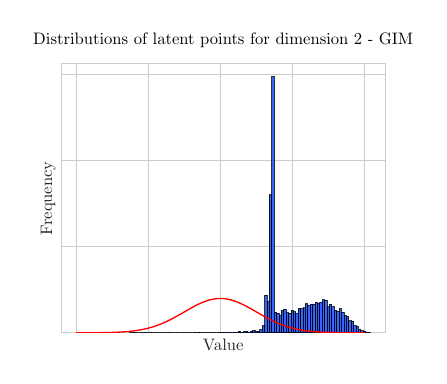
\begin{tikzpicture}[scale=0.6]

\definecolor{blue262255}{RGB}{2,62,255}
\definecolor{darkslategray38}{RGB}{38,38,38}
\definecolor{lightgray204}{RGB}{204,204,204}

\begin{axis}[
axis line style={lightgray204},
tick align=outside,
title={Distributions of latent points for dimension 2 - GIM},
x grid style={lightgray204},
xlabel=\textcolor{darkslategray38}{Value},
xmajorgrids,
xmajorticks=false,
xmin=-4.40780231952667, xmax=4.56384871006012,
xtick style={color=darkslategray38},
y grid style={lightgray204},
ylabel=\textcolor{darkslategray38}{Frequency},
ymajorgrids,
ymajorticks=false,
ymin=0, ymax=3.12677248557322,
ytick style={color=darkslategray38}
]
\draw[draw=black,fill=blue262255,opacity=0.8,line width=0.48pt] (axis cs:-2.50747537612915,0) rectangle (axis cs:-2.44084024429321,0.00199456388819194);
\draw[draw=black,fill=blue262255,opacity=0.8,line width=0.48pt] (axis cs:-2.44084024429321,0) rectangle (axis cs:-2.3742048740387,0);
\draw[draw=black,fill=blue262255,opacity=0.8,line width=0.48pt] (axis cs:-2.3742048740387,0) rectangle (axis cs:-2.30756974220276,0.00199456388819194);
\draw[draw=black,fill=blue262255,opacity=0.8,line width=0.48pt] (axis cs:-2.30756974220276,0) rectangle (axis cs:-2.24093461036682,0);
\draw[draw=black,fill=blue262255,opacity=0.8,line width=0.48pt] (axis cs:-2.24093437194824,0) rectangle (axis cs:-2.17429900169373,0);
\draw[draw=black,fill=blue262255,opacity=0.8,line width=0.48pt] (axis cs:-2.1742992401123,0) rectangle (axis cs:-2.10766410827637,0);
\draw[draw=black,fill=blue262255,opacity=0.8,line width=0.48pt] (axis cs:-2.10766410827637,0) rectangle (axis cs:-2.04102873802185,0.00199455675172543);
\draw[draw=black,fill=blue262255,opacity=0.8,line width=0.48pt] (axis cs:-2.04102873802185,0) rectangle (axis cs:-1.97439360618591,0);
\draw[draw=black,fill=blue262255,opacity=0.8,line width=0.48pt] (axis cs:-1.97439360618591,0) rectangle (axis cs:-1.90775847434998,0.00199456388819194);
\draw[draw=black,fill=blue262255,opacity=0.8,line width=0.48pt] (axis cs:-1.90775847434998,0) rectangle (axis cs:-1.84112334251404,0);
\draw[draw=black,fill=blue262255,opacity=0.8,line width=0.48pt] (axis cs:-1.84112310409546,0) rectangle (axis cs:-1.77448797225952,0.0019945603199523);
\draw[draw=black,fill=blue262255,opacity=0.8,line width=0.48pt] (axis cs:-1.77448797225952,0) rectangle (axis cs:-1.70785284042358,0);
\draw[draw=black,fill=blue262255,opacity=0.8,line width=0.48pt] (axis cs:-1.70785272121429,0) rectangle (axis cs:-1.64121758937836,0);
\draw[draw=black,fill=blue262255,opacity=0.8,line width=0.48pt] (axis cs:-1.64121747016907,0) rectangle (axis cs:-1.57458233833313,0.0019945603199523);
\draw[draw=black,fill=blue262255,opacity=0.8,line width=0.48pt] (axis cs:-1.57458233833313,0) rectangle (axis cs:-1.50794720649719,0);
\draw[draw=black,fill=blue262255,opacity=0.8,line width=0.48pt] (axis cs:-1.50794696807861,0) rectangle (axis cs:-1.44131183624268,0.0019945603199523);
\draw[draw=black,fill=blue262255,opacity=0.8,line width=0.48pt] (axis cs:-1.44131183624268,0) rectangle (axis cs:-1.37467670440674,0);
\draw[draw=black,fill=blue262255,opacity=0.8,line width=0.48pt] (axis cs:-1.37467670440674,0) rectangle (axis cs:-1.3080415725708,0);
\draw[draw=black,fill=blue262255,opacity=0.8,line width=0.48pt] (axis cs:-1.30804133415222,0) rectangle (axis cs:-1.24140620231628,0);
\draw[draw=black,fill=blue262255,opacity=0.8,line width=0.48pt] (axis cs:-1.24140620231628,0) rectangle (axis cs:-1.17477107048035,0);
\draw[draw=black,fill=blue262255,opacity=0.8,line width=0.48pt] (axis cs:-1.17477107048035,0) rectangle (axis cs:-1.10813593864441,0);
\draw[draw=black,fill=blue262255,opacity=0.8,line width=0.48pt] (axis cs:-1.10813570022583,0) rectangle (axis cs:-1.04150056838989,0);
\draw[draw=black,fill=blue262255,opacity=0.8,line width=0.48pt] (axis cs:-1.04150056838989,0) rectangle (axis cs:-0.974865436553955,0);
\draw[draw=black,fill=blue262255,opacity=0.8,line width=0.48pt] (axis cs:-0.974865317344666,0) rectangle (axis cs:-0.908230185508728,0);
\draw[draw=black,fill=blue262255,opacity=0.8,line width=0.48pt] (axis cs:-0.908230066299438,0) rectangle (axis cs:-0.841594934463501,0);
\draw[draw=black,fill=blue262255,opacity=0.8,line width=0.48pt] (axis cs:-0.841594934463501,0) rectangle (axis cs:-0.774959802627563,0);
\draw[draw=black,fill=blue262255,opacity=0.8,line width=0.48pt] (axis cs:-0.774959683418274,0) rectangle (axis cs:-0.708324551582336,0);
\draw[draw=black,fill=blue262255,opacity=0.8,line width=0.48pt] (axis cs:-0.708324432373047,0) rectangle (axis cs:-0.641689300537109,0.00199456210407052);
\draw[draw=black,fill=blue262255,opacity=0.8,line width=0.48pt] (axis cs:-0.641689240932465,0) rectangle (axis cs:-0.575054109096527,0.00598368095985689);
\draw[draw=black,fill=blue262255,opacity=0.8,line width=0.48pt] (axis cs:-0.575054049491882,0) rectangle (axis cs:-0.508418917655945,0.00199456210407052);
\draw[draw=black,fill=blue262255,opacity=0.8,line width=0.48pt] (axis cs:-0.508418798446655,0) rectangle (axis cs:-0.441783666610718,0);
\draw[draw=black,fill=blue262255,opacity=0.8,line width=0.48pt] (axis cs:-0.441783607006073,0) rectangle (axis cs:-0.375148475170135,0.00199456121201101);
\draw[draw=black,fill=blue262255,opacity=0.8,line width=0.48pt] (axis cs:-0.375148355960846,0) rectangle (axis cs:-0.308513224124908,0);
\draw[draw=black,fill=blue262255,opacity=0.8,line width=0.48pt] (axis cs:-0.308513164520264,0) rectangle (axis cs:-0.241878032684326,0);
\draw[draw=black,fill=blue262255,opacity=0.8,line width=0.48pt] (axis cs:-0.241877928376198,0) rectangle (axis cs:-0.17524279654026,0.00199456121201101);
\draw[draw=black,fill=blue262255,opacity=0.8,line width=0.48pt] (axis cs:-0.175242707133293,0) rectangle (axis cs:-0.108607575297356,0);
\draw[draw=black,fill=blue262255,opacity=0.8,line width=0.48pt] (axis cs:-0.10860750079155,0) rectangle (axis cs:-0.0419723689556122,0);
\draw[draw=black,fill=blue262255,opacity=0.8,line width=0.48pt] (axis cs:-0.041972279548645,0) rectangle (axis cs:0.0246628522872925,0.00598368363603303);
\draw[draw=black,fill=blue262255,opacity=0.8,line width=0.48pt] (axis cs:0.024662934243679,0) rectangle (axis cs:0.0912980660796165,0.00398912287005163);
\draw[draw=black,fill=blue262255,opacity=0.8,line width=0.48pt] (axis cs:0.0912981480360031,0) rectangle (axis cs:0.157933279871941,0.00398912287005163);
\draw[draw=black,fill=blue262255,opacity=0.8,line width=0.48pt] (axis cs:0.157933369278908,0) rectangle (axis cs:0.224568501114845,0.00199456121201101);
\draw[draw=black,fill=blue262255,opacity=0.8,line width=0.48pt] (axis cs:0.224568605422974,0) rectangle (axis cs:0.291203737258911,0.00398912242402202);
\draw[draw=black,fill=blue262255,opacity=0.8,line width=0.48pt] (axis cs:0.291203796863556,0) rectangle (axis cs:0.357838928699493,0.00199456121201101);
\draw[draw=black,fill=blue262255,opacity=0.8,line width=0.48pt] (axis cs:0.357839047908783,0) rectangle (axis cs:0.42447417974472,0.00997280606005505);
\draw[draw=black,fill=blue262255,opacity=0.8,line width=0.48pt] (axis cs:0.424474239349365,0) rectangle (axis cs:0.491109371185303,0.00797824484804404);
\draw[draw=black,fill=blue262255,opacity=0.8,line width=0.48pt] (axis cs:0.491109490394592,0) rectangle (axis cs:0.55774462223053,0.0179510589366347);
\draw[draw=black,fill=blue262255,opacity=0.8,line width=0.48pt] (axis cs:0.557744681835175,0) rectangle (axis cs:0.624379813671112,0.00797824127980919);
\draw[draw=black,fill=blue262255,opacity=0.8,line width=0.48pt] (axis cs:0.624379873275757,0) rectangle (axis cs:0.691015005111694,0.0139619347284936);
\draw[draw=black,fill=blue262255,opacity=0.8,line width=0.48pt] (axis cs:0.691015124320984,0) rectangle (axis cs:0.757650256156921,0.0179510428795707);
\draw[draw=black,fill=blue262255,opacity=0.8,line width=0.48pt] (axis cs:0.757650375366211,0) rectangle (axis cs:0.824285507202148,0.00997281052035261);
\draw[draw=black,fill=blue262255,opacity=0.8,line width=0.48pt] (axis cs:0.824285507202148,0) rectangle (axis cs:0.890920639038086,0.0199456210407052);
\draw[draw=black,fill=blue262255,opacity=0.8,line width=0.48pt] (axis cs:0.890920758247375,0) rectangle (axis cs:0.957555890083313,0.0299184047992845);
\draw[draw=black,fill=blue262255,opacity=0.8,line width=0.48pt] (axis cs:0.957556009292603,0) rectangle (axis cs:1.02419114112854,0.0139619347284936);
\draw[draw=black,fill=blue262255,opacity=0.8,line width=0.48pt] (axis cs:1.02419114112854,0) rectangle (axis cs:1.09082627296448,0.019945603199523);
\draw[draw=black,fill=blue262255,opacity=0.8,line width=0.48pt] (axis cs:1.09082651138306,0) rectangle (axis cs:1.15746164321899,0.0378966460790937);
\draw[draw=black,fill=blue262255,opacity=0.8,line width=0.48pt] (axis cs:1.15746164321899,0) rectangle (axis cs:1.22409677505493,0.0837716833040613);
\draw[draw=black,fill=blue262255,opacity=0.8,line width=0.48pt] (axis cs:1.22409677505493,0) rectangle (axis cs:1.29073190689087,0.438803270389506);
\draw[draw=black,fill=blue262255,opacity=0.8,line width=0.48pt] (axis cs:1.29073214530945,0) rectangle (axis cs:1.35736727714539,0.368993659191175);
\draw[draw=black,fill=blue262255,opacity=0.8,line width=0.48pt] (axis cs:1.35736727714539,0) rectangle (axis cs:1.42400240898132,1.60562392999451);
\draw[draw=black,fill=blue262255,opacity=0.8,line width=0.48pt] (axis cs:1.42400240898132,0) rectangle (axis cs:1.49063754081726,2.97787855768878);
\draw[draw=black,fill=blue262255,opacity=0.8,line width=0.48pt] (axis cs:1.49063777923584,0) rectangle (axis cs:1.55727291107178,0.237352678074323);
\draw[draw=black,fill=blue262255,opacity=0.8,line width=0.48pt] (axis cs:1.55727291107178,0) rectangle (axis cs:1.62390804290771,0.22538531615461);
\draw[draw=black,fill=blue262255,opacity=0.8,line width=0.48pt] (axis cs:1.623908162117,0) rectangle (axis cs:1.69054329395294,0.203445516595577);
\draw[draw=black,fill=blue262255,opacity=0.8,line width=0.48pt] (axis cs:1.69054341316223,0) rectangle (axis cs:1.75717854499817,0.263281962233703);
\draw[draw=black,fill=blue262255,opacity=0.8,line width=0.48pt] (axis cs:1.75717854499817,0) rectangle (axis cs:1.82381367683411,0.271260203513512);
\draw[draw=black,fill=blue262255,opacity=0.8,line width=0.48pt] (axis cs:1.82381391525269,0) rectangle (axis cs:1.89044904708862,0.235358117754371);
\draw[draw=black,fill=blue262255,opacity=0.8,line width=0.48pt] (axis cs:1.89044904708862,0) rectangle (axis cs:1.95708417892456,0.227380283253881);
\draw[draw=black,fill=blue262255,opacity=0.8,line width=0.48pt] (axis cs:1.95708417892456,0) rectangle (axis cs:2.0237193107605,0.261287869353144);
\draw[draw=black,fill=blue262255,opacity=0.8,line width=0.48pt] (axis cs:2.0237193107605,0) rectangle (axis cs:2.09035468101501,0.245330480462227);
\draw[draw=black,fill=blue262255,opacity=0.8,line width=0.48pt] (axis cs:2.09035468101501,0) rectangle (axis cs:2.15698981285095,0.223391155477497);
\draw[draw=black,fill=blue262255,opacity=0.8,line width=0.48pt] (axis cs:2.15699005126953,0) rectangle (axis cs:2.22362542152405,0.289210729000187);
\draw[draw=black,fill=blue262255,opacity=0.8,line width=0.48pt] (axis cs:2.22362518310547,0) rectangle (axis cs:2.29026031494141,0.281233508235063);
\draw[draw=black,fill=blue262255,opacity=0.8,line width=0.48pt] (axis cs:2.29026031494141,0) rectangle (axis cs:2.35689544677734,0.293200891564215);
\draw[draw=black,fill=blue262255,opacity=0.8,line width=0.48pt] (axis cs:2.35689544677734,0) rectangle (axis cs:2.42353081703186,0.339074647793323);
\draw[draw=black,fill=blue262255,opacity=0.8,line width=0.48pt] (axis cs:2.42353081703186,0) rectangle (axis cs:2.4901659488678,0.315141094334326);
\draw[draw=black,fill=blue262255,opacity=0.8,line width=0.48pt] (axis cs:2.4901659488678,0) rectangle (axis cs:2.55680108070374,0.329103041551669);
\draw[draw=black,fill=blue262255,opacity=0.8,line width=0.48pt] (axis cs:2.55680131912231,0) rectangle (axis cs:2.62343668937683,0.329101864034695);
\draw[draw=black,fill=blue262255,opacity=0.8,line width=0.48pt] (axis cs:2.62343645095825,0) rectangle (axis cs:2.69007158279419,0.359021499874548);
\draw[draw=black,fill=blue262255,opacity=0.8,line width=0.48pt] (axis cs:2.69007158279419,0) rectangle (axis cs:2.75670671463013,0.343064988769013);
\draw[draw=black,fill=blue262255,opacity=0.8,line width=0.48pt] (axis cs:2.75670671463013,0) rectangle (axis cs:2.82334208488464,0.355031101807126);
\draw[draw=black,fill=blue262255,opacity=0.8,line width=0.48pt] (axis cs:2.82334208488464,0) rectangle (axis cs:2.88997721672058,0.382956266532852);
\draw[draw=black,fill=blue262255,opacity=0.8,line width=0.48pt] (axis cs:2.88997745513916,0) rectangle (axis cs:2.95661282539368,0.376971226076106);
\draw[draw=black,fill=blue262255,opacity=0.8,line width=0.48pt] (axis cs:2.9566125869751,0) rectangle (axis cs:3.02324771881104,0.301179147116982);
\draw[draw=black,fill=blue262255,opacity=0.8,line width=0.48pt] (axis cs:3.02324771881104,0) rectangle (axis cs:3.08988285064697,0.331097605439861);
\draw[draw=black,fill=blue262255,opacity=0.8,line width=0.48pt] (axis cs:3.08988285064697,0) rectangle (axis cs:3.15651822090149,0.303172626262265);
\draw[draw=black,fill=blue262255,opacity=0.8,line width=0.48pt] (axis cs:3.15651822090149,0) rectangle (axis cs:3.22315335273743,0.263282433241336);
\draw[draw=black,fill=blue262255,opacity=0.8,line width=0.48pt] (axis cs:3.22315335273743,0) rectangle (axis cs:3.28978848457336,0.249320486023992);
\draw[draw=black,fill=blue262255,opacity=0.8,line width=0.48pt] (axis cs:3.28978872299194,0) rectangle (axis cs:3.35642409324646,0.27923794524156);
\draw[draw=black,fill=blue262255,opacity=0.8,line width=0.48pt] (axis cs:3.35642385482788,0) rectangle (axis cs:3.42305898666382,0.23735310269484);
\draw[draw=black,fill=blue262255,opacity=0.8,line width=0.48pt] (axis cs:3.42305898666382,0) rectangle (axis cs:3.48969411849976,0.203445516595577);
\draw[draw=black,fill=blue262255,opacity=0.8,line width=0.48pt] (axis cs:3.48969411849976,0) rectangle (axis cs:3.55632948875427,0.18748833466219);
\draw[draw=black,fill=blue262255,opacity=0.8,line width=0.48pt] (axis cs:3.55632948875427,0) rectangle (axis cs:3.62296462059021,0.139619472173436);
\draw[draw=black,fill=blue262255,opacity=0.8,line width=0.48pt] (axis cs:3.62296462059021,0) rectangle (axis cs:3.68959975242615,0.13363578050886);
\draw[draw=black,fill=blue262255,opacity=0.8,line width=0.48pt] (axis cs:3.68959999084473,0) rectangle (axis cs:3.75623536109924,0.0837713835724679);
\draw[draw=black,fill=blue262255,opacity=0.8,line width=0.48pt] (axis cs:3.75623512268066,0) rectangle (axis cs:3.8228702545166,0.0777879916394855);
\draw[draw=black,fill=blue262255,opacity=0.8,line width=0.48pt] (axis cs:3.8228702545166,0) rectangle (axis cs:3.88950562477112,0.0398911350345085);
\draw[draw=black,fill=blue262255,opacity=0.8,line width=0.48pt] (axis cs:3.88950562477112,0) rectangle (axis cs:3.95614075660706,0.0259293305464952);
\draw[draw=black,fill=blue262255,opacity=0.8,line width=0.48pt] (axis cs:3.95614099502563,0) rectangle (axis cs:4.02277660369873,0.0199455675172543);
\draw[draw=black,fill=blue262255,opacity=0.8,line width=0.48pt] (axis cs:4.02277612686157,0) rectangle (axis cs:4.08941125869751,0.00598369166457581);
\draw[draw=black,fill=blue262255,opacity=0.8,line width=0.48pt] (axis cs:4.08941125869751,0) rectangle (axis cs:4.15604639053345,0.00598369166457581);
\addplot [thick, red]
table {%
-4 0.000133830225764885
-3.99199199199199 0.000138182046410498
-3.98398398398398 0.000142666228042307
-3.97597597597598 0.000147286481503254
-3.96796796796797 0.000152046611333821
-3.95995995995996 0.000156950517814782
-3.95195195195195 0.00016200219904485
-3.94394394394394 0.00016720575305353
-3.93593593593594 0.000172565379949496
-3.92792792792793 0.00017808538410479
-3.91991991991992 0.000183770176375138
-3.91191191191191 0.000189624276356684
-3.9039039039039 0.000195652314679408
-3.8958958958959 0.000201859035337517
-3.88788788788789 0.000208249298057069
-3.87987987987988 0.000214828080701088
-3.87187187187187 0.000221600481712426
-3.86386386386386 0.0002285717225946
-3.85585585585586 0.000235747150430845
-3.84784784784785 0.000243132240441603
-3.83983983983984 0.000250732598580649
-3.83183183183183 0.000258553964170059
-3.82382382382382 0.000266602212574213
-3.81581581581582 0.000274883357912987
-3.80780780780781 0.000283403555814325
-3.7997997997998 0.000292169106206322
-3.79179179179179 0.000301186456148957
-3.78378378378378 0.0003104622027056
-3.77577577577578 0.000320003095854415
-3.76776776776777 0.000329816041439723
-3.75975975975976 0.000339908104163431
-3.75175175175175 0.00035028651061658
-3.74374374374374 0.000360958652351047
-3.73573573573574 0.000371932088991451
-3.72772772772773 0.000383214551387261
-3.71971971971972 0.000394813944805093
-3.71171171171171 0.000406738352161197
-3.7037037037037 0.000418996037294058
-3.6956956956957 0.00043159544827708
-3.68768768768769 0.00044454522077123
-3.67967967967968 0.000457854181417586
-3.67167167167167 0.000471531351269624
-3.66366366366366 0.000485585949265103
-3.65565565565566 0.000500027395737409
-3.64764764764765 0.000514865315966112
-3.63963963963964 0.000530109543766577
-3.63163163163163 0.000545770125118336
-3.62362362362362 0.000561857321831991
-3.61561561561562 0.00057838161525435
-3.60760760760761 0.000595353710011453
-3.5995995995996 0.000612784537789192
-3.59159159159159 0.000630685261151105
-3.58358358358358 0.000649067277392973
-3.57557557557558 0.000667942222433796
-3.56756756756757 0.000687321974742665
-3.55955955955956 0.000707218659301081
-3.55155155155155 0.000727644651600166
-3.54354354354354 0.000748612581672245
-3.53553553553554 0.000770135338156225
-3.52752752752753 0.000792226072396121
-3.51951951951952 0.00081489820257214
-3.51151151151151 0.000838165417863603
-3.5035035035035 0.000862041682643007
-3.4954954954955 0.000886541240700502
-3.48748748748749 0.00091167861949796
-3.47947947947948 0.000937468634451866
-3.47147147147147 0.000963926393244149
-3.46346346346346 0.000991067300160059
-3.45545545545546 0.0010189070604522
-3.44744744744745 0.00104746168472971
-3.43943943943944 0.0010767474933716
-3.43143143143143 0.00110678112096323
-3.42342342342342 0.00113757952075483
-3.41541541541542 0.00116915996914087
-3.40740740740741 0.00120154007015926
-3.3993993993994 0.00123473776000907
-3.39139139139139 0.00126877131158549
-3.38338338338338 0.00130365933903088
-3.37537537537538 0.00133942080230046
-3.36736736736737 0.00137607501174126
-3.35935935935936 0.001413641632683
-3.35135135135135 0.00145214069003938
-3.34334334334334 0.0014915925729182
-3.33533533533534 0.00153201803923895
-3.32732732732733 0.00157343822035606
-3.31931931931932 0.00161587462568624
-3.31131131131131 0.00165934914733831
-3.3033033033033 0.00170388406474362
-3.2952952952953 0.00174950204928538
-3.28728728728729 0.00179622616892505
-3.27927927927928 0.00184407989282385
-3.27127127127127 0.00189308709595757
-3.26326326326326 0.00194327206372255
-3.25525525525526 0.00199465949653091
-3.24724724724725 0.00204727451439301
-3.23923923923924 0.00210114266148476
-3.23123123123123 0.00215628991069791
-3.22322322322322 0.00221274266817093
-3.21521521521522 0.00227052777779815
-3.20720720720721 0.00232967252571501
-3.1991991991992 0.00239020464475689
-3.19119119119119 0.00245215231888918
-3.18318318318318 0.00251554418760605
-3.17517517517518 0.00258040935029545
-3.16716716716717 0.00264677737056774
-3.15915915915916 0.00271467828054534
-3.15115115115115 0.00278414258511061
-3.14314314314314 0.00285520126610952
-3.13513513513514 0.00292788578650791
-3.12712712712713 0.00300222809449793
-3.11911911911912 0.00307826062755151
-3.11111111111111 0.00315601631641804
-3.1031031031031 0.00323552858906328
-3.0950950950951 0.00331683137454643
-3.08708708708709 0.00339995910683238
-3.07907907907908 0.00348494672853595
-3.07107107107107 0.00357182969459489
-3.06306306306306 0.00366064397586864
-3.05505505505506 0.00375142606265932
-3.04704704704705 0.00384421296815189
-3.03903903903904 0.00393904223176991
-3.03103103103103 0.00403595192244368
-3.02302302302302 0.0041349806417872
-3.01501501501502 0.00423616752718052
-3.00700700700701 0.00433955225475399
-2.998998998999 0.00444517504227068
-2.99099099099099 0.00455307665190355
-2.98298298298298 0.00466329839290368
-2.97497497497497 0.00477588212415564
-2.96696696696697 0.00489087025661667
-2.95895895895896 0.00500830575563558
-2.95095095095095 0.00512823214314763
-2.94294294294294 0.00525069349974172
-2.93493493493493 0.00537573446659573
-2.92692692692693 0.00550340024727644
-2.91891891891892 0.00563373660939975
-2.91091091091091 0.0057667898861475
-2.9029029029029 0.00590260697763674
-2.89489489489489 0.00604123535213746
-2.88688688688689 0.00618272304713484
-2.87887887887888 0.00632711867023164
-2.87087087087087 0.00647447139988703
-2.86286286286286 0.00662483098598741
-2.85485485485485 0.0067782477502453
-2.84684684684685 0.0069347725864219
-2.83883883883884 0.00709445696036946
-2.83083083083083 0.00725735290988893
-2.82282282282282 0.00742351304439893
-2.81481481481481 0.00759299054441176
-2.80680680680681 0.0077658391608121
-2.7987987987988 0.00794211321393437
-2.79079079079079 0.00812186759243432
-2.78278278278278 0.00830515775195071
-2.77477477477477 0.00849203971355293
-2.76676676676677 0.00868257006197001
-2.75875875875876 0.00887680594359712
-2.75075075075075 0.00907480506427511
-2.74274274274274 0.00927662568683898
-2.73473473473473 0.00948232662843099
-2.72672672672673 0.00969196725757422
-2.71871871871872 0.00990560749100246
-2.71071071071071 0.0101233077902421
-2.7027027027027 0.0103451291579421
-2.69469469469469 0.0105711331339476
-2.68668668668669 0.0108013817911136
-2.67867867867868 0.011035937730854
-2.67067067067067 0.0112748640784219
-2.66266266266266 0.0115182244779185
-2.65465465465465 0.0117660830870247
-2.64664664664665 0.0120185045714526
-2.63863863863864 0.0122755540991133
-2.63063063063063 0.0125372973339956
-2.62262262262262 0.0128038004297541
-2.61461461461461 0.0130751300230007
-2.60660660660661 0.0133513532262973
-2.5985985985986 0.0136325376208454
-2.59059059059059 0.0139187512488692
-2.58258258258258 0.014210062605689
-2.57457457457457 0.0145065406314803
-2.56656656656657 0.0148082547027168
-2.55855855855856 0.0151152746232934
-2.55055055055055 0.0154276706153247
-2.54254254254254 0.0157455133096184
-2.53453453453453 0.0160688737358178
-2.52652652652653 0.016397823312213
-2.51851851851852 0.0167324338352151
-2.51051051051051 0.0170727774684938
-2.5025025025025 0.0174189267317727
-2.49449449449449 0.0177709544892815
-2.48648648648649 0.0181289339378627
-2.47847847847848 0.0184929385947284
-2.47047047047047 0.0188630422848682
-2.46246246246246 0.0192393191281025
-2.45445445445445 0.0196218435257817
-2.44644644644645 0.0200106901471285
-2.43843843843844 0.020405933915221
-2.43043043043043 0.0208076499926159
-2.42242242242242 0.0212159137666093
-2.41441441441441 0.0216308008341344
-2.40640640640641 0.0220523869862944
-2.3983983983984 0.0224807481925294
-2.39039039039039 0.022915960584417
-2.38238238238238 0.0233581004391047
-2.37437437437437 0.023807244162374
-2.36636636636637 0.0242634682713357
-2.35835835835836 0.0247268493767558
-2.35035035035035 0.0251974641650118
-2.34234234234234 0.0256753893796796
-2.33433433433433 0.0261607018027501
-2.32632632632633 0.0266534782354775
-2.31831831831832 0.0271537954788581
-2.31031031031031 0.0276617303137407
-2.3023023023023 0.0281773594805703
-2.29429429429429 0.0287007596587648
-2.28628628628629 0.0292320074457259
-2.27827827827828 0.029771179335487
-2.27027027027027 0.0303183516969979
-2.26226226226226 0.0308736007520491
-2.25425425425425 0.0314370025528369
-2.24624624624625 0.0320086329591723
-2.23823823823824 0.0325885676153351
-2.23023023023023 0.0331768819265761
-2.22222222222222 0.0337736510352706
-2.21421421421421 0.0343789497967251
-2.20620620620621 0.0349928527546413
-2.1981981981982 0.0356154341162401
-2.19019019019019 0.0362467677270497
-2.18218218218218 0.0368869270453615
-2.17417417417417 0.0375359851163567
-2.16616616616617 0.03819401454591
-2.15815815815816 0.0388610874740724
-2.15015015015015 0.03953727554824
-2.14214214214214 0.0402226498960119
-2.13413413413413 0.0409172810977437
-2.12612612612613 0.0416212391588003
-2.11811811811812 0.0423345934815158
-2.11011011011011 0.0430574128368641
-2.1021021021021 0.043789765335848
-2.09409409409409 0.0445317184006117
-2.08608608608609 0.0452833387352837
-2.07807807807808 0.0460446922965577
-2.07007007007007 0.0468158442640166
-2.06206206206206 0.0475968590102091
-2.05405405405405 0.0483878000704834
-2.04604604604605 0.0491887301125894
-2.03803803803804 0.0499997109060533
-2.03003003003003 0.0508208032913361
-2.02202202202202 0.0516520671487823
-2.01401401401401 0.0524935613673682
-2.00600600600601 0.053345343813258
-1.997997997998 0.0542074712981785
-1.98998998998999 0.0550799995476186
-1.98198198198198 0.0559629831688668
-1.97397397397397 0.0568564756188931
-1.96596596596597 0.0577605291720876
-1.95795795795796 0.0586751948878651
-1.94994994994995 0.0596005225781457
-1.94194194194194 0.0605365607747232
-1.93393393393393 0.0614833566965309
-1.92592592592593 0.062440956216817
-1.91791791791792 0.06340940383024
-1.90990990990991 0.0643887426198963
-1.9019019019019 0.0653790142242912
-1.89389389389389 0.0663802588042656
-1.88588588588589 0.0673925150098903
-1.87787787787788 0.0684158199473405
-1.86986986986987 0.0694502091457625
-1.86186186186186 0.0704957165241465
-1.85385385385385 0.0715523743582165
-1.84584584584585 0.0726202132473521
-1.83783783783784 0.0736992620815557
-1.82982982982983 0.0747895480084762
-1.82182182182182 0.0758910964005057
-1.81381381381381 0.0770039308219614
-1.80580580580581 0.0781280729963669
-1.7977977977978 0.0792635427738473
-1.78978978978979 0.0804103580986525
-1.78178178178178 0.0815685349768227
-1.77377377377377 0.0827380874440109
-1.76576576576577 0.0839190275334777
-1.75775775775776 0.0851113652442723
-1.74974974974975 0.086315108509615
-1.74174174174174 0.0875302631654975
-1.73373373373373 0.0887568329195139
-1.72572572572573 0.0899948193199405
-1.71771771771772 0.0912442217250772
-1.70970970970971 0.0925050372728685
-1.7017017017017 0.0937772608508177
-1.69369369369369 0.0950608850662112
-1.68568568568569 0.0963559002166691
-1.67767767767768 0.0976622942610365
-1.66966966966967 0.0989800527906321
-1.66166166166166 0.100309159000872
-1.65365365365365 0.10164959366328
-1.64564564564565 0.103001335097907
-1.63763763763764 0.10436435914617
-1.62962962962963 0.105738639144131
-1.62162162162162 0.107124145896225
-1.61361361361361 0.108520847649465
-1.60560560560561 0.10992871006813
-1.5975975975976 0.111347696208955
-1.58958958958959 0.112777766496842
-1.58158158158158 0.114218878701105
-1.57357357357357 0.115670987912262
-1.56556556556557 0.117134046519405
-1.55755755755756 0.11860800418814
-1.54954954954955 0.120092807839133
-1.54154154154154 0.121588401627275
-1.53353353353353 0.123094726921466
-1.52552552552553 0.124611722285057
-1.51751751751752 0.12613932345695
-1.50950950950951 0.127677463333369
-1.5015015015015 0.129226071950339
-1.49349349349349 0.130785076466857
-1.48548548548549 0.132354401148798
-1.47747747747748 0.133933967353555
-1.46946946946947 0.13552369351543
-1.46146146146146 0.137123495131801
-1.45345345345345 0.13873328475006
-1.44544544544545 0.140352971955359
-1.43743743743744 0.141982463359159
-1.42942942942943 0.143621662588612
-1.42142142142142 0.14527047027677
-1.41341341341341 0.146928784053658
-1.40540540540541 0.148596498538208
-1.3973973973974 0.150273505331067
-1.38938938938939 0.151959693008306
-1.38138138138138 0.153654947116025
-1.37337337337337 0.155359150165875
-1.36536536536537 0.157072181631514
-1.35735735735736 0.158793917945997
-1.34934934934935 0.160524232500121
-1.34134134134134 0.16226299564173
-1.33333333333333 0.164010074675994
-1.32532532532533 0.165765333866673
-1.31731731731732 0.167528634438376
-1.30930930930931 0.169299834579821
-1.3013013013013 0.17107878944811
-1.29329329329329 0.172865351174024
-1.28528528528529 0.174659368868355
-1.27727727727728 0.176460688629273
-1.26926926926927 0.178269153550739
-1.26126126126126 0.180084603731981
-1.25325325325325 0.181906876288021
-1.24524524524525 0.183735805361283
-1.23723723723724 0.185571222134271
-1.22922922922923 0.187412954843324
-1.22122122122122 0.18926082879347
-1.21321321321321 0.191114666374361
-1.20520520520521 0.192974287077311
-1.1971971971972 0.194839507513435
-1.18918918918919 0.19671014143289
-1.18118118118118 0.198585999745227
-1.17317317317317 0.200466890540856
-1.16516516516517 0.202352619113618
-1.15715715715716 0.204242987984477
-1.14914914914915 0.206137796926331
-1.14114114114114 0.208036842989938
-1.13313313313313 0.209939920530956
-1.12512512512513 0.21184682123811
-1.11711711711712 0.21375733416247
-1.10910910910911 0.215671245747847
-1.1011011011011 0.217588339862305
-1.09309309309309 0.219508397830784
-1.08508508508509 0.221431198468836
-1.07707707707708 0.223356518117463
-1.06906906906907 0.225284130679063
-1.06106106106106 0.22721380765447
-1.05305305305305 0.229145318181096
-1.04504504504505 0.231078429072154
-1.03703703703704 0.233012904856966
-1.02902902902903 0.234948507822352
-1.02102102102102 0.236884998055083
-1.01301301301301 0.238822133485401
-1.00500500500501 0.24075966993159
-0.996996996996997 0.242697361145593
-0.988988988988989 0.244634958859672
-0.980980980980981 0.246572212834085
-0.972972972972973 0.248508870905785
-0.964964964964965 0.250444679038131
-0.956956956956957 0.252379381371581
-0.948948948948949 0.254312720275385
-0.940940940940941 0.256244436400228
-0.932932932932933 0.258174268731856
-0.924924924924925 0.260101954645624
-0.916916916916917 0.262027229961987
-0.908908908908909 0.263949829002911
-0.900900900900901 0.265869484649172
-0.892892892892893 0.267785928398552
-0.884884884884885 0.269698890424904
-0.876876876876877 0.271608099638066
-0.868868868868869 0.273513283744617
-0.860860860860861 0.275414169309444
-0.852852852852853 0.277310481818125
-0.844844844844845 0.279201945740075
-0.836836836836837 0.281088284592474
-0.828828828828829 0.28296922100493
-0.820820820820821 0.284844476784867
-0.812812812812813 0.286713772983616
-0.804804804804805 0.288576829963198
-0.796796796796797 0.290433367463758
-0.788788788788789 0.292283104671645
-0.780780780780781 0.294125760288111
-0.772772772772773 0.295961052598604
-0.764764764764765 0.29778869954263
-0.756756756756757 0.299608418784177
-0.748748748748749 0.301419927782648
-0.740740740740741 0.303222943864308
-0.732732732732733 0.305017184294205
-0.724724724724725 0.306802366348536
-0.716716716716717 0.308578207387456
-0.708708708708709 0.310344424928268
-0.700700700700701 0.312100736719007
-0.692692692692693 0.313846860812361
-0.684684684684685 0.31558251563992
-0.676676676676677 0.317307420086723
-0.668668668668669 0.319021293566066
-0.660660660660661 0.320723856094559
-0.652652652652653 0.322414828367396
-0.644644644644645 0.324093931833804
-0.636636636636636 0.325760888772662
-0.628628628628629 0.327415422368237
-0.620620620620621 0.329057256786028
-0.612612612612613 0.330686117248681
-0.604604604604605 0.33230173011195
-0.596596596596596 0.333903822940662
-0.588588588588589 0.335492124584683
-0.580580580580581 0.337066365254824
-0.572572572572573 0.338626276598684
-0.564564564564565 0.340171591776383
-0.556556556556556 0.341702045536168
-0.548548548548549 0.343217374289848
-0.54054054054054 0.344717316188045
-0.532532532532533 0.346201611195215
-0.524524524524525 0.347670001164422
-0.516516516516516 0.349122229911825
-0.508508508508509 0.350558043290856
-0.5005005005005 0.351977189266054
-0.492492492492492 0.353379417986526
-0.484484484484485 0.354764481859011
-0.476476476476476 0.356132135620502
-0.468468468468469 0.357482136410418
-0.46046046046046 0.358814243842273
-0.452452452452452 0.360128220074839
-0.444444444444445 0.361423829882744
-0.436436436436436 0.362700840726495
-0.428428428428429 0.363959022821904
-0.42042042042042 0.365198149208855
-0.412412412412412 0.366417995819425
-0.404404404404405 0.3676183415453
-0.396396396396396 0.368798968304465
-0.388388388388389 0.369959661107154
-0.38038038038038 0.37110020812101
-0.372372372372372 0.372220400735444
-0.364364364364365 0.373320033625156
-0.356356356356356 0.374398904812801
-0.348348348348348 0.375456815730761
-0.34034034034034 0.376493571282005
-0.332332332332332 0.377508979900006
-0.324324324324325 0.378502853607702
-0.316316316316316 0.379475008075448
-0.308308308308308 0.380425262677969
-0.3003003003003 0.38135344055026
-0.292292292292292 0.382259368642425
-0.284284284284285 0.38314287777343
-0.276276276276276 0.384003802683735
-0.268268268268268 0.3848419820868
-0.26026026026026 0.385657258719425
-0.252252252252252 0.386449479390916
-0.244244244244244 0.387218495031049
-0.236236236236236 0.387964160736805
-0.228228228228228 0.38868633581787
-0.22022022022022 0.389384883840873
-0.212212212212212 0.390059672672329
-0.204204204204204 0.390710574520297
-0.196196196196196 0.391337465974705
-0.188188188188188 0.39194022804635
-0.18018018018018 0.392518746204527
-0.172172172172172 0.393072910413305
-0.164164164164164 0.393602615166401
-0.156156156156156 0.394107759520658
-0.148148148148148 0.394588247128102
-0.14014014014014 0.395043986266573
-0.132132132132132 0.3954748898689
-0.124124124124124 0.395880875550626
-0.116116116116116 0.396261865636259
-0.108108108108108 0.396617787184037
-0.1001001001001 0.396948572009207
-0.0920920920920922 0.397254156705792
-0.084084084084084 0.397534482666846
-0.0760760760760761 0.39778949610319
-0.0680680680680683 0.39801914806061
-0.06006006006006 0.398223394435522
-0.0520520520520522 0.398402195989086
-0.0440440440440439 0.398555518359772
-0.0360360360360361 0.398683332074364
-0.0280280280280278 0.398785612557403
-0.02002002002002 0.398862340139061
-0.0120120120120122 0.398913500061449
-0.00400400400400391 0.398939082483343
0.00400400400400436 0.398939082483343
0.0120120120120122 0.398913500061449
0.02002002002002 0.398862340139061
0.0280280280280278 0.398785612557403
0.0360360360360357 0.398683332074364
0.0440440440440444 0.398555518359772
0.0520520520520522 0.398402195989086
0.06006006006006 0.398223394435522
0.0680680680680679 0.39801914806061
0.0760760760760757 0.39778949610319
0.0840840840840844 0.397534482666846
0.0920920920920922 0.397254156705792
0.1001001001001 0.396948572009207
0.108108108108108 0.396617787184037
0.116116116116116 0.396261865636259
0.124124124124124 0.395880875550626
0.132132132132132 0.3954748898689
0.14014014014014 0.395043986266573
0.148148148148148 0.394588247128102
0.156156156156156 0.394107759520658
0.164164164164164 0.393602615166401
0.172172172172172 0.393072910413305
0.18018018018018 0.392518746204527
0.188188188188188 0.39194022804635
0.196196196196196 0.391337465974705
0.204204204204204 0.390710574520297
0.212212212212212 0.390059672672329
0.22022022022022 0.389384883840873
0.228228228228228 0.388686335817871
0.236236236236236 0.387964160736805
0.244244244244245 0.387218495031049
0.252252252252252 0.386449479390916
0.26026026026026 0.385657258719425
0.268268268268268 0.3848419820868
0.276276276276276 0.384003802683735
0.284284284284285 0.38314287777343
0.292292292292292 0.382259368642425
0.3003003003003 0.38135344055026
0.308308308308308 0.380425262677969
0.316316316316316 0.379475008075448
0.324324324324325 0.378502853607702
0.332332332332332 0.377508979900006
0.34034034034034 0.376493571282005
0.348348348348348 0.375456815730762
0.356356356356356 0.374398904812801
0.364364364364365 0.373320033625156
0.372372372372372 0.372220400735444
0.38038038038038 0.37110020812101
0.388388388388388 0.369959661107154
0.396396396396397 0.368798968304465
0.404404404404405 0.3676183415453
0.412412412412412 0.366417995819425
0.42042042042042 0.365198149208855
0.428428428428428 0.363959022821904
0.436436436436437 0.362700840726495
0.444444444444445 0.361423829882744
0.452452452452452 0.360128220074839
0.46046046046046 0.358814243842273
0.468468468468468 0.357482136410418
0.476476476476477 0.356132135620502
0.484484484484485 0.354764481859011
0.492492492492492 0.353379417986526
0.5005005005005 0.351977189266054
0.508508508508508 0.350558043290856
0.516516516516517 0.349122229911825
0.524524524524525 0.347670001164422
0.532532532532533 0.346201611195215
0.54054054054054 0.344717316188045
0.548548548548548 0.343217374289848
0.556556556556557 0.341702045536168
0.564564564564565 0.340171591776383
0.572572572572573 0.338626276598684
0.58058058058058 0.337066365254824
0.588588588588588 0.335492124584683
0.596596596596597 0.333903822940662
0.604604604604605 0.33230173011195
0.612612612612613 0.330686117248681
0.62062062062062 0.329057256786028
0.628628628628628 0.327415422368237
0.636636636636637 0.325760888772662
0.644644644644645 0.324093931833804
0.652652652652653 0.322414828367396
0.66066066066066 0.32072385609456
0.668668668668668 0.319021293566066
0.676676676676677 0.317307420086723
0.684684684684685 0.31558251563992
0.692692692692693 0.313846860812361
0.7007007007007 0.312100736719007
0.708708708708708 0.310344424928268
0.716716716716717 0.308578207387456
0.724724724724725 0.306802366348536
0.732732732732733 0.305017184294205
0.74074074074074 0.303222943864308
0.748748748748748 0.301419927782648
0.756756756756757 0.299608418784177
0.764764764764765 0.29778869954263
0.772772772772773 0.295961052598604
0.780780780780781 0.294125760288111
0.788788788788788 0.292283104671645
0.796796796796797 0.290433367463758
0.804804804804805 0.288576829963198
0.812812812812813 0.286713772983616
0.820820820820821 0.284844476784867
0.828828828828828 0.282969221004931
0.836836836836837 0.281088284592474
0.844844844844845 0.279201945740075
0.852852852852853 0.277310481818125
0.860860860860861 0.275414169309444
0.868868868868869 0.273513283744617
0.876876876876877 0.271608099638066
0.884884884884885 0.269698890424904
0.892892892892893 0.267785928398552
0.900900900900901 0.265869484649172
0.908908908908909 0.263949829002911
0.916916916916917 0.262027229961987
0.924924924924925 0.260101954645624
0.932932932932933 0.258174268731856
0.940940940940941 0.256244436400228
0.948948948948949 0.254312720275384
0.956956956956957 0.252379381371581
0.964964964964965 0.250444679038131
0.972972972972973 0.248508870905785
0.980980980980981 0.246572212834085
0.988988988988989 0.244634958859672
0.996996996996997 0.242697361145593
1.00500500500501 0.24075966993159
1.01301301301301 0.238822133485401
1.02102102102102 0.236884998055083
1.02902902902903 0.234948507822352
1.03703703703704 0.233012904856966
1.04504504504505 0.231078429072154
1.05305305305305 0.229145318181096
1.06106106106106 0.22721380765447
1.06906906906907 0.225284130679062
1.07707707707708 0.223356518117463
1.08508508508509 0.221431198468836
1.09309309309309 0.219508397830784
1.1011011011011 0.217588339862305
1.10910910910911 0.215671245747847
1.11711711711712 0.21375733416247
1.12512512512513 0.21184682123811
1.13313313313313 0.209939920530956
1.14114114114114 0.208036842989938
1.14914914914915 0.206137796926331
1.15715715715716 0.204242987984477
1.16516516516517 0.202352619113618
1.17317317317317 0.200466890540856
1.18118118118118 0.198585999745228
1.18918918918919 0.19671014143289
1.1971971971972 0.194839507513435
1.20520520520521 0.192974287077311
1.21321321321321 0.191114666374361
1.22122122122122 0.18926082879347
1.22922922922923 0.187412954843324
1.23723723723724 0.185571222134271
1.24524524524525 0.183735805361283
1.25325325325325 0.181906876288021
1.26126126126126 0.180084603731981
1.26926926926927 0.178269153550739
1.27727727727728 0.176460688629273
1.28528528528529 0.174659368868355
1.29329329329329 0.172865351174024
1.3013013013013 0.17107878944811
1.30930930930931 0.169299834579821
1.31731731731732 0.167528634438376
1.32532532532533 0.165765333866673
1.33333333333333 0.164010074675994
1.34134134134134 0.16226299564173
1.34934934934935 0.160524232500121
1.35735735735736 0.158793917945997
1.36536536536537 0.157072181631514
1.37337337337337 0.155359150165875
1.38138138138138 0.153654947116025
1.38938938938939 0.151959693008306
1.3973973973974 0.150273505331067
1.40540540540541 0.148596498538208
1.41341341341341 0.146928784053658
1.42142142142142 0.14527047027677
1.42942942942943 0.143621662588612
1.43743743743744 0.141982463359159
1.44544544544545 0.140352971955359
1.45345345345345 0.13873328475006
1.46146146146146 0.137123495131801
1.46946946946947 0.13552369351543
1.47747747747748 0.133933967353555
1.48548548548549 0.132354401148798
1.49349349349349 0.130785076466857
1.5015015015015 0.129226071950339
1.50950950950951 0.127677463333369
1.51751751751752 0.12613932345695
1.52552552552553 0.124611722285057
1.53353353353353 0.123094726921466
1.54154154154154 0.121588401627275
1.54954954954955 0.120092807839133
1.55755755755756 0.11860800418814
1.56556556556557 0.117134046519405
1.57357357357357 0.115670987912262
1.58158158158158 0.114218878701105
1.58958958958959 0.112777766496842
1.5975975975976 0.111347696208955
1.60560560560561 0.10992871006813
1.61361361361361 0.108520847649465
1.62162162162162 0.107124145896225
1.62962962962963 0.105738639144131
1.63763763763764 0.10436435914617
1.64564564564565 0.103001335097907
1.65365365365365 0.10164959366328
1.66166166166166 0.100309159000872
1.66966966966967 0.0989800527906321
1.67767767767768 0.0976622942610365
1.68568568568569 0.0963559002166692
1.69369369369369 0.0950608850662112
1.7017017017017 0.0937772608508176
1.70970970970971 0.0925050372728685
1.71771771771772 0.0912442217250772
1.72572572572573 0.0899948193199405
1.73373373373373 0.088756832919514
1.74174174174174 0.0875302631654974
1.74974974974975 0.086315108509615
1.75775775775776 0.0851113652442723
1.76576576576577 0.0839190275334778
1.77377377377377 0.082738087444011
1.78178178178178 0.0815685349768226
1.78978978978979 0.0804103580986525
1.7977977977978 0.0792635427738473
1.80580580580581 0.0781280729963669
1.81381381381381 0.0770039308219615
1.82182182182182 0.0758910964005057
1.82982982982983 0.0747895480084762
1.83783783783784 0.0736992620815557
1.84584584584585 0.0726202132473522
1.85385385385385 0.0715523743582165
1.86186186186186 0.0704957165241465
1.86986986986987 0.0694502091457625
1.87787787787788 0.0684158199473405
1.88588588588589 0.0673925150098903
1.89389389389389 0.0663802588042655
1.9019019019019 0.0653790142242912
1.90990990990991 0.0643887426198963
1.91791791791792 0.06340940383024
1.92592592592593 0.0624409562168171
1.93393393393393 0.0614833566965309
1.94194194194194 0.0605365607747232
1.94994994994995 0.0596005225781457
1.95795795795796 0.0586751948878651
1.96596596596597 0.0577605291720876
1.97397397397397 0.056856475618893
1.98198198198198 0.0559629831688668
1.98998998998999 0.0550799995476186
1.997997997998 0.0542074712981785
2.00600600600601 0.0533453438132581
2.01401401401401 0.0524935613673681
2.02202202202202 0.0516520671487823
2.03003003003003 0.0508208032913361
2.03803803803804 0.0499997109060533
2.04604604604605 0.0491887301125894
2.05405405405405 0.0483878000704834
2.06206206206206 0.0475968590102091
2.07007007007007 0.0468158442640166
2.07807807807808 0.0460446922965577
2.08608608608609 0.0452833387352837
2.09409409409409 0.0445317184006117
2.1021021021021 0.043789765335848
2.11011011011011 0.0430574128368641
2.11811811811812 0.0423345934815158
2.12612612612613 0.0416212391588004
2.13413413413413 0.0409172810977437
2.14214214214214 0.0402226498960119
2.15015015015015 0.03953727554824
2.15815815815816 0.0388610874740724
2.16616616616617 0.03819401454591
2.17417417417417 0.0375359851163567
2.18218218218218 0.0368869270453615
2.19019019019019 0.0362467677270497
2.1981981981982 0.0356154341162401
2.20620620620621 0.0349928527546413
2.21421421421421 0.0343789497967251
2.22222222222222 0.0337736510352706
2.23023023023023 0.0331768819265761
2.23823823823824 0.0325885676153351
2.24624624624625 0.0320086329591724
2.25425425425425 0.0314370025528369
2.26226226226226 0.0308736007520491
2.27027027027027 0.0303183516969979
2.27827827827828 0.029771179335487
2.28628628628629 0.0292320074457259
2.29429429429429 0.0287007596587648
2.3023023023023 0.0281773594805703
2.31031031031031 0.0276617303137407
2.31831831831832 0.0271537954788581
2.32632632632633 0.0266534782354776
2.33433433433433 0.0261607018027501
2.34234234234234 0.0256753893796796
2.35035035035035 0.0251974641650118
2.35835835835836 0.0247268493767558
2.36636636636637 0.0242634682713357
2.37437437437437 0.023807244162374
2.38238238238238 0.0233581004391047
2.39039039039039 0.022915960584417
2.3983983983984 0.0224807481925294
2.40640640640641 0.0220523869862944
2.41441441441441 0.0216308008341344
2.42242242242242 0.0212159137666093
2.43043043043043 0.0208076499926159
2.43843843843844 0.020405933915221
2.44644644644645 0.0200106901471285
2.45445445445445 0.0196218435257817
2.46246246246246 0.0192393191281025
2.47047047047047 0.0188630422848682
2.47847847847848 0.0184929385947284
2.48648648648649 0.0181289339378626
2.49449449449449 0.0177709544892815
2.5025025025025 0.0174189267317727
2.51051051051051 0.0170727774684938
2.51851851851852 0.0167324338352152
2.52652652652653 0.016397823312213
2.53453453453453 0.0160688737358178
2.54254254254254 0.0157455133096184
2.55055055055055 0.0154276706153247
2.55855855855856 0.0151152746232934
2.56656656656657 0.0148082547027168
2.57457457457457 0.0145065406314803
2.58258258258258 0.014210062605689
2.59059059059059 0.0139187512488692
2.5985985985986 0.0136325376208454
2.60660660660661 0.0133513532262973
2.61461461461461 0.0130751300230007
2.62262262262262 0.0128038004297541
2.63063063063063 0.0125372973339956
2.63863863863864 0.0122755540991133
2.64664664664665 0.0120185045714526
2.65465465465465 0.0117660830870247
2.66266266266266 0.0115182244779185
2.67067067067067 0.0112748640784219
2.67867867867868 0.011035937730854
2.68668668668669 0.0108013817911136
2.69469469469469 0.0105711331339476
2.7027027027027 0.0103451291579421
2.71071071071071 0.0101233077902421
2.71871871871872 0.00990560749100247
2.72672672672673 0.00969196725757422
2.73473473473473 0.00948232662843099
2.74274274274274 0.00927662568683898
2.75075075075075 0.00907480506427511
2.75875875875876 0.00887680594359712
2.76676676676677 0.00868257006197001
2.77477477477477 0.00849203971355293
2.78278278278278 0.00830515775195071
2.79079079079079 0.00812186759243432
2.7987987987988 0.00794211321393438
2.80680680680681 0.0077658391608121
2.81481481481481 0.00759299054441176
2.82282282282282 0.00742351304439893
2.83083083083083 0.00725735290988893
2.83883883883884 0.00709445696036947
2.84684684684685 0.0069347725864219
2.85485485485485 0.0067782477502453
2.86286286286286 0.00662483098598741
2.87087087087087 0.00647447139988703
2.87887887887888 0.00632711867023165
2.88688688688689 0.00618272304713484
2.89489489489489 0.00604123535213746
2.9029029029029 0.00590260697763674
2.91091091091091 0.0057667898861475
2.91891891891892 0.00563373660939975
2.92692692692693 0.00550340024727644
2.93493493493493 0.00537573446659573
2.94294294294294 0.00525069349974172
2.95095095095095 0.00512823214314764
2.95895895895896 0.00500830575563558
2.96696696696697 0.00489087025661667
2.97497497497497 0.00477588212415564
2.98298298298298 0.00466329839290368
2.99099099099099 0.00455307665190356
2.998998998999 0.00444517504227067
3.00700700700701 0.00433955225475399
3.01501501501502 0.00423616752718052
3.02302302302302 0.0041349806417872
3.03103103103103 0.00403595192244368
3.03903903903904 0.00393904223176991
3.04704704704705 0.00384421296815189
3.05505505505506 0.00375142606265932
3.06306306306306 0.00366064397586864
3.07107107107107 0.00357182969459489
3.07907907907908 0.00348494672853594
3.08708708708709 0.00339995910683238
3.0950950950951 0.00331683137454643
3.1031031031031 0.00323552858906328
3.11111111111111 0.00315601631641805
3.11911911911912 0.00307826062755151
3.12712712712713 0.00300222809449793
3.13513513513514 0.00292788578650791
3.14314314314314 0.00285520126610952
3.15115115115115 0.00278414258511062
3.15915915915916 0.00271467828054533
3.16716716716717 0.00264677737056774
3.17517517517518 0.00258040935029545
3.18318318318318 0.00251554418760605
3.19119119119119 0.00245215231888919
3.1991991991992 0.00239020464475689
3.20720720720721 0.00232967252571501
3.21521521521522 0.00227052777779815
3.22322322322322 0.00221274266817093
3.23123123123123 0.00215628991069792
3.23923923923924 0.00210114266148476
3.24724724724725 0.00204727451439301
3.25525525525526 0.00199465949653091
3.26326326326326 0.00194327206372255
3.27127127127127 0.00189308709595757
3.27927927927928 0.00184407989282385
3.28728728728729 0.00179622616892505
3.2952952952953 0.00174950204928538
3.3033033033033 0.00170388406474362
3.31131131131131 0.00165934914733832
3.31931931931932 0.00161587462568624
3.32732732732733 0.00157343822035606
3.33533533533534 0.00153201803923895
3.34334334334334 0.0014915925729182
3.35135135135135 0.00145214069003938
3.35935935935936 0.001413641632683
3.36736736736737 0.00137607501174126
3.37537537537538 0.00133942080230046
3.38338338338338 0.00130365933903089
3.39139139139139 0.00126877131158549
3.3993993993994 0.00123473776000907
3.40740740740741 0.00120154007015926
3.41541541541542 0.00116915996914087
3.42342342342342 0.00113757952075483
3.43143143143143 0.00110678112096324
3.43943943943944 0.0010767474933716
3.44744744744745 0.00104746168472971
3.45545545545546 0.0010189070604522
3.46346346346346 0.000991067300160061
3.47147147147147 0.000963926393244148
3.47947947947948 0.000937468634451866
3.48748748748749 0.00091167861949796
3.4954954954955 0.000886541240700502
3.5035035035035 0.000862041682643008
3.51151151151151 0.000838165417863601
3.51951951951952 0.00081489820257214
3.52752752752753 0.000792226072396121
3.53553553553554 0.000770135338156225
3.54354354354354 0.000748612581672247
3.55155155155155 0.000727644651600165
3.55955955955956 0.000707218659301081
3.56756756756757 0.000687321974742665
3.57557557557558 0.000667942222433796
3.58358358358358 0.000649067277392974
3.59159159159159 0.000630685261151104
3.5995995995996 0.000612784537789192
3.60760760760761 0.000595353710011453
3.61561561561562 0.00057838161525435
3.62362362362362 0.000561857321831992
3.63163163163163 0.000545770125118335
3.63963963963964 0.000530109543766577
3.64764764764765 0.000514865315966112
3.65565565565566 0.000500027395737409
3.66366366366366 0.000485585949265104
3.67167167167167 0.000471531351269623
3.67967967967968 0.000457854181417586
3.68768768768769 0.00044454522077123
3.6956956956957 0.00043159544827708
3.7037037037037 0.000418996037294059
3.71171171171171 0.000406738352161196
3.71971971971972 0.000394813944805093
3.72772772772773 0.000383214551387261
3.73573573573574 0.000371932088991452
3.74374374374374 0.000360958652351047
3.75175175175175 0.000350286510616579
3.75975975975976 0.000339908104163431
3.76776776776777 0.000329816041439723
3.77577577577578 0.000320003095854415
3.78378378378378 0.0003104622027056
3.79179179179179 0.000301186456148956
3.7997997997998 0.000292169106206322
3.80780780780781 0.000283403555814325
3.81581581581582 0.000274883357912987
3.82382382382382 0.000266602212574214
3.83183183183183 0.000258553964170059
3.83983983983984 0.000250732598580649
3.84784784784785 0.000243132240441603
3.85585585585586 0.000235747150430845
3.86386386386386 0.000228571722594601
3.87187187187187 0.000221600481712426
3.87987987987988 0.000214828080701088
3.88788788788789 0.000208249298057069
3.8958958958959 0.000201859035337517
3.9039039039039 0.000195652314679408
3.91191191191191 0.000189624276356684
3.91991991991992 0.000183770176375138
3.92792792792793 0.00017808538410479
3.93593593593594 0.000172565379949497
3.94394394394394 0.00016720575305353
3.95195195195195 0.00016200219904485
3.95995995995996 0.000156950517814782
3.96796796796797 0.000152046611333821
3.97597597597598 0.000147286481503255
3.98398398398398 0.000142666228042307
3.99199199199199 0.000138182046410498
4 0.000133830225764885
};
\end{axis}

\end{tikzpicture}
%		\end{subfigure}
%		\hfill
%		\begin{subfigure}[b]{0.25\textwidth}
%			\centering
%			% This file was created with tikzplotlib v0.10.1.
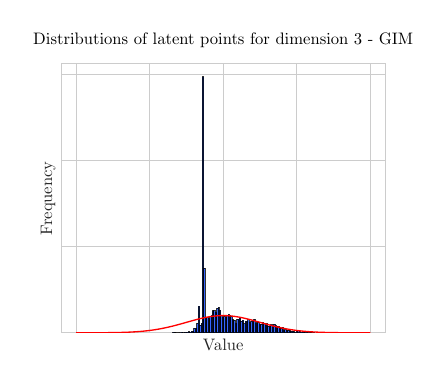
\begin{tikzpicture}[scale=0.6]

\definecolor{blue262255}{RGB}{2,62,255}
\definecolor{darkslategray38}{RGB}{38,38,38}
\definecolor{lightgray204}{RGB}{204,204,204}

\begin{axis}[
axis line style={lightgray204},
tick align=outside,
title={Distributions of latent points for dimension 3 - GIM},
x grid style={lightgray204},
xlabel=\textcolor{darkslategray38}{Value},
xmajorgrids,
xmajorticks=false,
xmin=-4.4, xmax=4.4,
xtick style={color=darkslategray38},
y grid style={lightgray204},
ylabel=\textcolor{darkslategray38}{Frequency},
ymajorgrids,
ymajorticks=false,
ymin=0, ymax=6.23497985999709,
ytick style={color=darkslategray38}
]
\draw[draw=black,fill=blue262255,opacity=0.8,line width=0.48pt] (axis cs:-1.37576580047607,0) rectangle (axis cs:-1.33713388442993,0.00688073703028979);
\draw[draw=black,fill=blue262255,opacity=0.8,line width=0.48pt] (axis cs:-1.33713388442993,0) rectangle (axis cs:-1.29850196838379,0.00344036851514489);
\draw[draw=black,fill=blue262255,opacity=0.8,line width=0.48pt] (axis cs:-1.29850196838379,0) rectangle (axis cs:-1.25987005233765,0.00344036851514489);
\draw[draw=black,fill=blue262255,opacity=0.8,line width=0.48pt] (axis cs:-1.25987005233765,0) rectangle (axis cs:-1.2212381362915,0);
\draw[draw=black,fill=blue262255,opacity=0.8,line width=0.48pt] (axis cs:-1.2212381362915,0) rectangle (axis cs:-1.18260622024536,0.00344036851514489);
\draw[draw=black,fill=blue262255,opacity=0.8,line width=0.48pt] (axis cs:-1.18260622024536,0) rectangle (axis cs:-1.14397442340851,0);
\draw[draw=black,fill=blue262255,opacity=0.8,line width=0.48pt] (axis cs:-1.14397442340851,0) rectangle (axis cs:-1.10534250736237,0.0103211055454347);
\draw[draw=black,fill=blue262255,opacity=0.8,line width=0.48pt] (axis cs:-1.10534250736237,0) rectangle (axis cs:-1.06671059131622,0.00344036851514489);
\draw[draw=black,fill=blue262255,opacity=0.8,line width=0.48pt] (axis cs:-1.06671059131622,0) rectangle (axis cs:-1.02807867527008,0.00344036851514489);
\draw[draw=black,fill=blue262255,opacity=0.8,line width=0.48pt] (axis cs:-1.02807867527008,0) rectangle (axis cs:-0.989446759223938,0.0103211055454347);
\draw[draw=black,fill=blue262255,opacity=0.8,line width=0.48pt] (axis cs:-0.989446759223938,0) rectangle (axis cs:-0.950814843177795,0.0172018425757245);
\draw[draw=black,fill=blue262255,opacity=0.8,line width=0.48pt] (axis cs:-0.950814843177795,0) rectangle (axis cs:-0.912182927131653,0.0240825796060143);
\draw[draw=black,fill=blue262255,opacity=0.8,line width=0.48pt] (axis cs:-0.912182927131653,0) rectangle (axis cs:-0.87355101108551,0.0172018691162486);
\draw[draw=black,fill=blue262255,opacity=0.8,line width=0.48pt] (axis cs:-0.873551070690155,0) rectangle (axis cs:-0.834919154644012,0.0412844221817387);
\draw[draw=black,fill=blue262255,opacity=0.8,line width=0.48pt] (axis cs:-0.834919154644012,0) rectangle (axis cs:-0.79628723859787,0.030963316636304);
\draw[draw=black,fill=blue262255,opacity=0.8,line width=0.48pt] (axis cs:-0.79628723859787,0) rectangle (axis cs:-0.757655322551727,0.0997706869392019);
\draw[draw=black,fill=blue262255,opacity=0.8,line width=0.48pt] (axis cs:-0.757655322551727,0) rectangle (axis cs:-0.719023406505585,0.106651423969492);
\draw[draw=black,fill=blue262255,opacity=0.8,line width=0.48pt] (axis cs:-0.719023466110229,0) rectangle (axis cs:-0.680391550064087,0.216743550864732);
\draw[draw=black,fill=blue262255,opacity=0.8,line width=0.48pt] (axis cs:-0.680391550064087,0) rectangle (axis cs:-0.641759634017944,0.612385595695791);
\draw[draw=black,fill=blue262255,opacity=0.8,line width=0.48pt] (axis cs:-0.641759634017944,0) rectangle (axis cs:-0.603127717971802,0.182339531302679);
\draw[draw=black,fill=blue262255,opacity=0.8,line width=0.48pt] (axis cs:-0.603127717971802,0) rectangle (axis cs:-0.564495801925659,0.227064321999563);
\draw[draw=black,fill=blue262255,opacity=0.8,line width=0.48pt] (axis cs:-0.564495801925659,0) rectangle (axis cs:-0.525863885879517,5.93807605714009);
\draw[draw=black,fill=blue262255,opacity=0.8,line width=0.48pt] (axis cs:-0.525863885879517,0) rectangle (axis cs:-0.487231969833374,1.49312108743074);
\draw[draw=black,fill=blue262255,opacity=0.8,line width=0.48pt] (axis cs:-0.487232029438019,0) rectangle (axis cs:-0.448600113391876,0.354358230427111);
\draw[draw=black,fill=blue262255,opacity=0.8,line width=0.48pt] (axis cs:-0.448600113391876,0) rectangle (axis cs:-0.409968197345734,0.357798325575069);
\draw[draw=black,fill=blue262255,opacity=0.8,line width=0.48pt] (axis cs:-0.409968197345734,0) rectangle (axis cs:-0.371336281299591,0.326835008938765);
\draw[draw=black,fill=blue262255,opacity=0.8,line width=0.48pt] (axis cs:-0.371336281299591,0) rectangle (axis cs:-0.332704365253448,0.375000457442283);
\draw[draw=black,fill=blue262255,opacity=0.8,line width=0.48pt] (axis cs:-0.332704395055771,0) rectangle (axis cs:-0.294072479009628,0.395642379241663);
\draw[draw=black,fill=blue262255,opacity=0.8,line width=0.48pt] (axis cs:-0.294072508811951,0) rectangle (axis cs:-0.255440592765808,0.516055675379288);
\draw[draw=black,fill=blue262255,opacity=0.8,line width=0.48pt] (axis cs:-0.255440592765808,0) rectangle (axis cs:-0.216808676719666,0.509174540241444);
\draw[draw=black,fill=blue262255,opacity=0.8,line width=0.48pt] (axis cs:-0.216808676719666,0) rectangle (axis cs:-0.178176760673523,0.467890298535061);
\draw[draw=black,fill=blue262255,opacity=0.8,line width=0.48pt] (axis cs:-0.178176790475845,0) rectangle (axis cs:-0.139544874429703,0.574541763642317);
\draw[draw=black,fill=blue262255,opacity=0.8,line width=0.48pt] (axis cs:-0.139544874429703,0) rectangle (axis cs:-0.10091295838356,0.588303129550364);
\draw[draw=black,fill=blue262255,opacity=0.8,line width=0.48pt] (axis cs:-0.100912973284721,0) rectangle (axis cs:-0.0622810572385788,0.522936165582822);
\draw[draw=black,fill=blue262255,opacity=0.8,line width=0.48pt] (axis cs:-0.0622810646891594,0) rectangle (axis cs:-0.0236491486430168,0.395642493697529);
\draw[draw=black,fill=blue262255,opacity=0.8,line width=0.48pt] (axis cs:-0.0236491616815329,0) rectangle (axis cs:0.0149827543646097,0.36467916810381);
\draw[draw=black,fill=blue262255,opacity=0.8,line width=0.48pt] (axis cs:0.0149827413260937,0) rectangle (axis cs:0.0536146573722363,0.378440646145463);
\draw[draw=black,fill=blue262255,opacity=0.8,line width=0.48pt] (axis cs:0.0536146461963654,0) rectangle (axis cs:0.0922465622425079,0.364679203269974);
\draw[draw=black,fill=blue262255,opacity=0.8,line width=0.48pt] (axis cs:0.0922465473413467,0) rectangle (axis cs:0.130878463387489,0.402523193902881);
\draw[draw=black,fill=blue262255,opacity=0.8,line width=0.48pt] (axis cs:0.130878448486328,0) rectangle (axis cs:0.169510364532471,0.436926969955534);
\draw[draw=black,fill=blue262255,opacity=0.8,line width=0.48pt] (axis cs:0.169510364532471,0) rectangle (axis cs:0.208142280578613,0.412844381060347);
\draw[draw=black,fill=blue262255,opacity=0.8,line width=0.48pt] (axis cs:0.208142250776291,0) rectangle (axis cs:0.246774166822433,0.378440682638652);
\draw[draw=black,fill=blue262255,opacity=0.8,line width=0.48pt] (axis cs:0.246774166822433,0) rectangle (axis cs:0.285406082868576,0.299312060817606);
\draw[draw=black,fill=blue262255,opacity=0.8,line width=0.48pt] (axis cs:0.285406053066254,0) rectangle (axis cs:0.324037969112396,0.292431549381597);
\draw[draw=black,fill=blue262255,opacity=0.8,line width=0.48pt] (axis cs:0.324037969112396,0) rectangle (axis cs:0.362669885158539,0.223623953484418);
\draw[draw=black,fill=blue262255,opacity=0.8,line width=0.48pt] (axis cs:0.362669885158539,0) rectangle (axis cs:0.401301801204681,0.313073534878185);
\draw[draw=black,fill=blue262255,opacity=0.8,line width=0.48pt] (axis cs:0.401301801204681,0) rectangle (axis cs:0.439933717250824,0.313073776396768);
\draw[draw=black,fill=blue262255,opacity=0.8,line width=0.48pt] (axis cs:0.439933687448502,0) rectangle (axis cs:0.478565603494644,0.344036851514489);
\draw[draw=black,fill=blue262255,opacity=0.8,line width=0.48pt] (axis cs:0.478565573692322,0) rectangle (axis cs:0.517197489738464,0.26834895119723);
\draw[draw=black,fill=blue262255,opacity=0.8,line width=0.48pt] (axis cs:0.517197489738464,0) rectangle (axis cs:0.555829405784607,0.292431323787316);
\draw[draw=black,fill=blue262255,opacity=0.8,line width=0.48pt] (axis cs:0.555829405784607,0) rectangle (axis cs:0.59446132183075,0.213302847938983);
\draw[draw=black,fill=blue262255,opacity=0.8,line width=0.48pt] (axis cs:0.59446132183075,0) rectangle (axis cs:0.633093237876892,0.264908375666157);
\draw[draw=black,fill=blue262255,opacity=0.8,line width=0.48pt] (axis cs:0.633093237876892,0) rectangle (axis cs:0.671725153923035,0.271789532036727);
\draw[draw=black,fill=blue262255,opacity=0.8,line width=0.48pt] (axis cs:0.67172509431839,0) rectangle (axis cs:0.710357010364532,0.319954271908475);
\draw[draw=black,fill=blue262255,opacity=0.8,line width=0.48pt] (axis cs:0.710357010364532,0) rectangle (axis cs:0.748988926410675,0.237385427544998);
\draw[draw=black,fill=blue262255,opacity=0.8,line width=0.48pt] (axis cs:0.748988926410675,0) rectangle (axis cs:0.787620842456818,0.275229481211592);
\draw[draw=black,fill=blue262255,opacity=0.8,line width=0.48pt] (axis cs:0.787620842456818,0) rectangle (axis cs:0.82625275850296,0.288990955272171);
\draw[draw=black,fill=blue262255,opacity=0.8,line width=0.48pt] (axis cs:0.826252698898315,0) rectangle (axis cs:0.864884614944458,0.319954765562223);
\draw[draw=black,fill=blue262255,opacity=0.8,line width=0.48pt] (axis cs:0.864884614944458,0) rectangle (axis cs:0.903516530990601,0.216743216454128);
\draw[draw=black,fill=blue262255,opacity=0.8,line width=0.48pt] (axis cs:0.903516530990601,0) rectangle (axis cs:0.942148447036743,0.233945059029853);
\draw[draw=black,fill=blue262255,opacity=0.8,line width=0.48pt] (axis cs:0.942148447036743,0) rectangle (axis cs:0.980780363082886,0.247706533090432);
\draw[draw=black,fill=blue262255,opacity=0.8,line width=0.48pt] (axis cs:0.980780363082886,0) rectangle (axis cs:1.01941227912903,0.202981742393549);
\draw[draw=black,fill=blue262255,opacity=0.8,line width=0.48pt] (axis cs:1.01941227912903,0) rectangle (axis cs:1.05804419517517,0.196101005363259);
\draw[draw=black,fill=blue262255,opacity=0.8,line width=0.48pt] (axis cs:1.05804419517517,0) rectangle (axis cs:1.09667611122131,0.230504690514708);
\draw[draw=black,fill=blue262255,opacity=0.8,line width=0.48pt] (axis cs:1.09667611122131,0) rectangle (axis cs:1.13530802726746,0.206422110908694);
\draw[draw=black,fill=blue262255,opacity=0.8,line width=0.48pt] (axis cs:1.13530802726746,0) rectangle (axis cs:1.17393982410431,0.168578577437174);
\draw[draw=black,fill=blue262255,opacity=0.8,line width=0.48pt] (axis cs:1.17393982410431,0) rectangle (axis cs:1.21257174015045,0.209862479423839);
\draw[draw=black,fill=blue262255,opacity=0.8,line width=0.48pt] (axis cs:1.21257174015045,0) rectangle (axis cs:1.25120365619659,0.15481658318152);
\draw[draw=black,fill=blue262255,opacity=0.8,line width=0.48pt] (axis cs:1.25120365619659,0) rectangle (axis cs:1.28983557224274,0.15481658318152);
\draw[draw=black,fill=blue262255,opacity=0.8,line width=0.48pt] (axis cs:1.28983557224274,0) rectangle (axis cs:1.32846748828888,0.185779899817824);
\draw[draw=black,fill=blue262255,opacity=0.8,line width=0.48pt] (axis cs:1.32846748828888,0) rectangle (axis cs:1.36709940433502,0.123853266545216);
\draw[draw=black,fill=blue262255,opacity=0.8,line width=0.48pt] (axis cs:1.36709940433502,0) rectangle (axis cs:1.40573132038116,0.199541373878404);
\draw[draw=black,fill=blue262255,opacity=0.8,line width=0.48pt] (axis cs:1.40573132038116,0) rectangle (axis cs:1.44436323642731,0.172018425757245);
\draw[draw=black,fill=blue262255,opacity=0.8,line width=0.48pt] (axis cs:1.44436323642731,0) rectangle (axis cs:1.48299515247345,0.158256951696665);
\draw[draw=black,fill=blue262255,opacity=0.8,line width=0.48pt] (axis cs:1.48299503326416,0) rectangle (axis cs:1.52162683010101,0.137615165254836);
\draw[draw=black,fill=blue262255,opacity=0.8,line width=0.48pt] (axis cs:1.5216269493103,0) rectangle (axis cs:1.56025886535645,0.116972529514926);
\draw[draw=black,fill=blue262255,opacity=0.8,line width=0.48pt] (axis cs:1.56025886535645,0) rectangle (axis cs:1.59889078140259,0.106651423969492);
\draw[draw=black,fill=blue262255,opacity=0.8,line width=0.48pt] (axis cs:1.59889078140259,0) rectangle (axis cs:1.63752269744873,0.134174372090651);
\draw[draw=black,fill=blue262255,opacity=0.8,line width=0.48pt] (axis cs:1.63752269744873,0) rectangle (axis cs:1.67615461349487,0.065367001787753);
\draw[draw=black,fill=blue262255,opacity=0.8,line width=0.48pt] (axis cs:1.67615461349487,0) rectangle (axis cs:1.71478652954102,0.0756881073331877);
\draw[draw=black,fill=blue262255,opacity=0.8,line width=0.48pt] (axis cs:1.71478652954102,0) rectangle (axis cs:1.75341844558716,0.0481651592120285);
\draw[draw=black,fill=blue262255,opacity=0.8,line width=0.48pt] (axis cs:1.75341844558716,0) rectangle (axis cs:1.7920503616333,0.0619266332726081);
\draw[draw=black,fill=blue262255,opacity=0.8,line width=0.48pt] (axis cs:1.7920503616333,0) rectangle (axis cs:1.83068227767944,0.0481651592120285);
\draw[draw=black,fill=blue262255,opacity=0.8,line width=0.48pt] (axis cs:1.83068227767944,0) rectangle (axis cs:1.86931419372559,0.0344036851514489);
\draw[draw=black,fill=blue262255,opacity=0.8,line width=0.48pt] (axis cs:1.86931419372559,0) rectangle (axis cs:1.90794610977173,0.0344036851514489);
\draw[draw=black,fill=blue262255,opacity=0.8,line width=0.48pt] (axis cs:1.90794610977173,0) rectangle (axis cs:1.94657790660858,0.0275230330509673);
\draw[draw=black,fill=blue262255,opacity=0.8,line width=0.48pt] (axis cs:1.94657790660858,0) rectangle (axis cs:1.98520982265472,0.0103211055454347);
\draw[draw=black,fill=blue262255,opacity=0.8,line width=0.48pt] (axis cs:1.98520994186401,0) rectangle (axis cs:2.02384185791016,0.0447246526867972);
\draw[draw=black,fill=blue262255,opacity=0.8,line width=0.48pt] (axis cs:2.02384185791016,0) rectangle (axis cs:2.0624737739563,0.0447247906968836);
\draw[draw=black,fill=blue262255,opacity=0.8,line width=0.48pt] (axis cs:2.0624737739563,0) rectangle (axis cs:2.10110569000244,0.0275229481211592);
\draw[draw=black,fill=blue262255,opacity=0.8,line width=0.48pt] (axis cs:2.10110569000244,0) rectangle (axis cs:2.13973736763,0.0103211692429873);
\draw[draw=black,fill=blue262255,opacity=0.8,line width=0.48pt] (axis cs:2.13973736763,0) rectangle (axis cs:2.17836928367615,0.0172018425757245);
\draw[draw=black,fill=blue262255,opacity=0.8,line width=0.48pt] (axis cs:2.17836928367615,0) rectangle (axis cs:2.21700119972229,0.0137614740605796);
\draw[draw=black,fill=blue262255,opacity=0.8,line width=0.48pt] (axis cs:2.21700119972229,0) rectangle (axis cs:2.25563311576843,0.00688073703028979);
\draw[draw=black,fill=blue262255,opacity=0.8,line width=0.48pt] (axis cs:2.25563311576843,0) rectangle (axis cs:2.29426503181458,0.0137614740605796);
\draw[draw=black,fill=blue262255,opacity=0.8,line width=0.48pt] (axis cs:2.29426503181458,0) rectangle (axis cs:2.33289694786072,0.00688073703028979);
\draw[draw=black,fill=blue262255,opacity=0.8,line width=0.48pt] (axis cs:2.33289694786072,0) rectangle (axis cs:2.37152886390686,0.0103211055454347);
\draw[draw=black,fill=blue262255,opacity=0.8,line width=0.48pt] (axis cs:2.37152886390686,0) rectangle (axis cs:2.410160779953,0.00344036851514489);
\draw[draw=black,fill=blue262255,opacity=0.8,line width=0.48pt] (axis cs:2.410160779953,0) rectangle (axis cs:2.44879269599915,0.00344036851514489);
\draw[draw=black,fill=blue262255,opacity=0.8,line width=0.48pt] (axis cs:2.44879269599915,0) rectangle (axis cs:2.48742461204529,0.00688073703028979);
\addplot [thick, red]
table {%
-4 0.000133830225764885
-3.99199199199199 0.000138182046410498
-3.98398398398398 0.000142666228042307
-3.97597597597598 0.000147286481503254
-3.96796796796797 0.000152046611333821
-3.95995995995996 0.000156950517814782
-3.95195195195195 0.00016200219904485
-3.94394394394394 0.00016720575305353
-3.93593593593594 0.000172565379949496
-3.92792792792793 0.00017808538410479
-3.91991991991992 0.000183770176375138
-3.91191191191191 0.000189624276356684
-3.9039039039039 0.000195652314679408
-3.8958958958959 0.000201859035337517
-3.88788788788789 0.000208249298057069
-3.87987987987988 0.000214828080701088
-3.87187187187187 0.000221600481712426
-3.86386386386386 0.0002285717225946
-3.85585585585586 0.000235747150430845
-3.84784784784785 0.000243132240441603
-3.83983983983984 0.000250732598580649
-3.83183183183183 0.000258553964170059
-3.82382382382382 0.000266602212574213
-3.81581581581582 0.000274883357912987
-3.80780780780781 0.000283403555814325
-3.7997997997998 0.000292169106206322
-3.79179179179179 0.000301186456148957
-3.78378378378378 0.0003104622027056
-3.77577577577578 0.000320003095854415
-3.76776776776777 0.000329816041439723
-3.75975975975976 0.000339908104163431
-3.75175175175175 0.00035028651061658
-3.74374374374374 0.000360958652351047
-3.73573573573574 0.000371932088991451
-3.72772772772773 0.000383214551387261
-3.71971971971972 0.000394813944805093
-3.71171171171171 0.000406738352161197
-3.7037037037037 0.000418996037294058
-3.6956956956957 0.00043159544827708
-3.68768768768769 0.00044454522077123
-3.67967967967968 0.000457854181417586
-3.67167167167167 0.000471531351269624
-3.66366366366366 0.000485585949265103
-3.65565565565566 0.000500027395737409
-3.64764764764765 0.000514865315966112
-3.63963963963964 0.000530109543766577
-3.63163163163163 0.000545770125118336
-3.62362362362362 0.000561857321831991
-3.61561561561562 0.00057838161525435
-3.60760760760761 0.000595353710011453
-3.5995995995996 0.000612784537789192
-3.59159159159159 0.000630685261151105
-3.58358358358358 0.000649067277392973
-3.57557557557558 0.000667942222433796
-3.56756756756757 0.000687321974742665
-3.55955955955956 0.000707218659301081
-3.55155155155155 0.000727644651600166
-3.54354354354354 0.000748612581672245
-3.53553553553554 0.000770135338156225
-3.52752752752753 0.000792226072396121
-3.51951951951952 0.00081489820257214
-3.51151151151151 0.000838165417863603
-3.5035035035035 0.000862041682643007
-3.4954954954955 0.000886541240700502
-3.48748748748749 0.00091167861949796
-3.47947947947948 0.000937468634451866
-3.47147147147147 0.000963926393244149
-3.46346346346346 0.000991067300160059
-3.45545545545546 0.0010189070604522
-3.44744744744745 0.00104746168472971
-3.43943943943944 0.0010767474933716
-3.43143143143143 0.00110678112096323
-3.42342342342342 0.00113757952075483
-3.41541541541542 0.00116915996914087
-3.40740740740741 0.00120154007015926
-3.3993993993994 0.00123473776000907
-3.39139139139139 0.00126877131158549
-3.38338338338338 0.00130365933903088
-3.37537537537538 0.00133942080230046
-3.36736736736737 0.00137607501174126
-3.35935935935936 0.001413641632683
-3.35135135135135 0.00145214069003938
-3.34334334334334 0.0014915925729182
-3.33533533533534 0.00153201803923895
-3.32732732732733 0.00157343822035606
-3.31931931931932 0.00161587462568624
-3.31131131131131 0.00165934914733831
-3.3033033033033 0.00170388406474362
-3.2952952952953 0.00174950204928538
-3.28728728728729 0.00179622616892505
-3.27927927927928 0.00184407989282385
-3.27127127127127 0.00189308709595757
-3.26326326326326 0.00194327206372255
-3.25525525525526 0.00199465949653091
-3.24724724724725 0.00204727451439301
-3.23923923923924 0.00210114266148476
-3.23123123123123 0.00215628991069791
-3.22322322322322 0.00221274266817093
-3.21521521521522 0.00227052777779815
-3.20720720720721 0.00232967252571501
-3.1991991991992 0.00239020464475689
-3.19119119119119 0.00245215231888918
-3.18318318318318 0.00251554418760605
-3.17517517517518 0.00258040935029545
-3.16716716716717 0.00264677737056774
-3.15915915915916 0.00271467828054534
-3.15115115115115 0.00278414258511061
-3.14314314314314 0.00285520126610952
-3.13513513513514 0.00292788578650791
-3.12712712712713 0.00300222809449793
-3.11911911911912 0.00307826062755151
-3.11111111111111 0.00315601631641804
-3.1031031031031 0.00323552858906328
-3.0950950950951 0.00331683137454643
-3.08708708708709 0.00339995910683238
-3.07907907907908 0.00348494672853595
-3.07107107107107 0.00357182969459489
-3.06306306306306 0.00366064397586864
-3.05505505505506 0.00375142606265932
-3.04704704704705 0.00384421296815189
-3.03903903903904 0.00393904223176991
-3.03103103103103 0.00403595192244368
-3.02302302302302 0.0041349806417872
-3.01501501501502 0.00423616752718052
-3.00700700700701 0.00433955225475399
-2.998998998999 0.00444517504227068
-2.99099099099099 0.00455307665190355
-2.98298298298298 0.00466329839290368
-2.97497497497497 0.00477588212415564
-2.96696696696697 0.00489087025661667
-2.95895895895896 0.00500830575563558
-2.95095095095095 0.00512823214314763
-2.94294294294294 0.00525069349974172
-2.93493493493493 0.00537573446659573
-2.92692692692693 0.00550340024727644
-2.91891891891892 0.00563373660939975
-2.91091091091091 0.0057667898861475
-2.9029029029029 0.00590260697763674
-2.89489489489489 0.00604123535213746
-2.88688688688689 0.00618272304713484
-2.87887887887888 0.00632711867023164
-2.87087087087087 0.00647447139988703
-2.86286286286286 0.00662483098598741
-2.85485485485485 0.0067782477502453
-2.84684684684685 0.0069347725864219
-2.83883883883884 0.00709445696036946
-2.83083083083083 0.00725735290988893
-2.82282282282282 0.00742351304439893
-2.81481481481481 0.00759299054441176
-2.80680680680681 0.0077658391608121
-2.7987987987988 0.00794211321393437
-2.79079079079079 0.00812186759243432
-2.78278278278278 0.00830515775195071
-2.77477477477477 0.00849203971355293
-2.76676676676677 0.00868257006197001
-2.75875875875876 0.00887680594359712
-2.75075075075075 0.00907480506427511
-2.74274274274274 0.00927662568683898
-2.73473473473473 0.00948232662843099
-2.72672672672673 0.00969196725757422
-2.71871871871872 0.00990560749100246
-2.71071071071071 0.0101233077902421
-2.7027027027027 0.0103451291579421
-2.69469469469469 0.0105711331339476
-2.68668668668669 0.0108013817911136
-2.67867867867868 0.011035937730854
-2.67067067067067 0.0112748640784219
-2.66266266266266 0.0115182244779185
-2.65465465465465 0.0117660830870247
-2.64664664664665 0.0120185045714526
-2.63863863863864 0.0122755540991133
-2.63063063063063 0.0125372973339956
-2.62262262262262 0.0128038004297541
-2.61461461461461 0.0130751300230007
-2.60660660660661 0.0133513532262973
-2.5985985985986 0.0136325376208454
-2.59059059059059 0.0139187512488692
-2.58258258258258 0.014210062605689
-2.57457457457457 0.0145065406314803
-2.56656656656657 0.0148082547027168
-2.55855855855856 0.0151152746232934
-2.55055055055055 0.0154276706153247
-2.54254254254254 0.0157455133096184
-2.53453453453453 0.0160688737358178
-2.52652652652653 0.016397823312213
-2.51851851851852 0.0167324338352151
-2.51051051051051 0.0170727774684938
-2.5025025025025 0.0174189267317727
-2.49449449449449 0.0177709544892815
-2.48648648648649 0.0181289339378627
-2.47847847847848 0.0184929385947284
-2.47047047047047 0.0188630422848682
-2.46246246246246 0.0192393191281025
-2.45445445445445 0.0196218435257817
-2.44644644644645 0.0200106901471285
-2.43843843843844 0.020405933915221
-2.43043043043043 0.0208076499926159
-2.42242242242242 0.0212159137666093
-2.41441441441441 0.0216308008341344
-2.40640640640641 0.0220523869862944
-2.3983983983984 0.0224807481925294
-2.39039039039039 0.022915960584417
-2.38238238238238 0.0233581004391047
-2.37437437437437 0.023807244162374
-2.36636636636637 0.0242634682713357
-2.35835835835836 0.0247268493767558
-2.35035035035035 0.0251974641650118
-2.34234234234234 0.0256753893796796
-2.33433433433433 0.0261607018027501
-2.32632632632633 0.0266534782354775
-2.31831831831832 0.0271537954788581
-2.31031031031031 0.0276617303137407
-2.3023023023023 0.0281773594805703
-2.29429429429429 0.0287007596587648
-2.28628628628629 0.0292320074457259
-2.27827827827828 0.029771179335487
-2.27027027027027 0.0303183516969979
-2.26226226226226 0.0308736007520491
-2.25425425425425 0.0314370025528369
-2.24624624624625 0.0320086329591723
-2.23823823823824 0.0325885676153351
-2.23023023023023 0.0331768819265761
-2.22222222222222 0.0337736510352706
-2.21421421421421 0.0343789497967251
-2.20620620620621 0.0349928527546413
-2.1981981981982 0.0356154341162401
-2.19019019019019 0.0362467677270497
-2.18218218218218 0.0368869270453615
-2.17417417417417 0.0375359851163567
-2.16616616616617 0.03819401454591
-2.15815815815816 0.0388610874740724
-2.15015015015015 0.03953727554824
-2.14214214214214 0.0402226498960119
-2.13413413413413 0.0409172810977437
-2.12612612612613 0.0416212391588003
-2.11811811811812 0.0423345934815158
-2.11011011011011 0.0430574128368641
-2.1021021021021 0.043789765335848
-2.09409409409409 0.0445317184006117
-2.08608608608609 0.0452833387352837
-2.07807807807808 0.0460446922965577
-2.07007007007007 0.0468158442640166
-2.06206206206206 0.0475968590102091
-2.05405405405405 0.0483878000704834
-2.04604604604605 0.0491887301125894
-2.03803803803804 0.0499997109060533
-2.03003003003003 0.0508208032913361
-2.02202202202202 0.0516520671487823
-2.01401401401401 0.0524935613673682
-2.00600600600601 0.053345343813258
-1.997997997998 0.0542074712981785
-1.98998998998999 0.0550799995476186
-1.98198198198198 0.0559629831688668
-1.97397397397397 0.0568564756188931
-1.96596596596597 0.0577605291720876
-1.95795795795796 0.0586751948878651
-1.94994994994995 0.0596005225781457
-1.94194194194194 0.0605365607747232
-1.93393393393393 0.0614833566965309
-1.92592592592593 0.062440956216817
-1.91791791791792 0.06340940383024
-1.90990990990991 0.0643887426198963
-1.9019019019019 0.0653790142242912
-1.89389389389389 0.0663802588042656
-1.88588588588589 0.0673925150098903
-1.87787787787788 0.0684158199473405
-1.86986986986987 0.0694502091457625
-1.86186186186186 0.0704957165241465
-1.85385385385385 0.0715523743582165
-1.84584584584585 0.0726202132473521
-1.83783783783784 0.0736992620815557
-1.82982982982983 0.0747895480084762
-1.82182182182182 0.0758910964005057
-1.81381381381381 0.0770039308219614
-1.80580580580581 0.0781280729963669
-1.7977977977978 0.0792635427738473
-1.78978978978979 0.0804103580986525
-1.78178178178178 0.0815685349768227
-1.77377377377377 0.0827380874440109
-1.76576576576577 0.0839190275334777
-1.75775775775776 0.0851113652442723
-1.74974974974975 0.086315108509615
-1.74174174174174 0.0875302631654975
-1.73373373373373 0.0887568329195139
-1.72572572572573 0.0899948193199405
-1.71771771771772 0.0912442217250772
-1.70970970970971 0.0925050372728685
-1.7017017017017 0.0937772608508177
-1.69369369369369 0.0950608850662112
-1.68568568568569 0.0963559002166691
-1.67767767767768 0.0976622942610365
-1.66966966966967 0.0989800527906321
-1.66166166166166 0.100309159000872
-1.65365365365365 0.10164959366328
-1.64564564564565 0.103001335097907
-1.63763763763764 0.10436435914617
-1.62962962962963 0.105738639144131
-1.62162162162162 0.107124145896225
-1.61361361361361 0.108520847649465
-1.60560560560561 0.10992871006813
-1.5975975975976 0.111347696208955
-1.58958958958959 0.112777766496842
-1.58158158158158 0.114218878701105
-1.57357357357357 0.115670987912262
-1.56556556556557 0.117134046519405
-1.55755755755756 0.11860800418814
-1.54954954954955 0.120092807839133
-1.54154154154154 0.121588401627275
-1.53353353353353 0.123094726921466
-1.52552552552553 0.124611722285057
-1.51751751751752 0.12613932345695
-1.50950950950951 0.127677463333369
-1.5015015015015 0.129226071950339
-1.49349349349349 0.130785076466857
-1.48548548548549 0.132354401148798
-1.47747747747748 0.133933967353555
-1.46946946946947 0.13552369351543
-1.46146146146146 0.137123495131801
-1.45345345345345 0.13873328475006
-1.44544544544545 0.140352971955359
-1.43743743743744 0.141982463359159
-1.42942942942943 0.143621662588612
-1.42142142142142 0.14527047027677
-1.41341341341341 0.146928784053658
-1.40540540540541 0.148596498538208
-1.3973973973974 0.150273505331067
-1.38938938938939 0.151959693008306
-1.38138138138138 0.153654947116025
-1.37337337337337 0.155359150165875
-1.36536536536537 0.157072181631514
-1.35735735735736 0.158793917945997
-1.34934934934935 0.160524232500121
-1.34134134134134 0.16226299564173
-1.33333333333333 0.164010074675994
-1.32532532532533 0.165765333866673
-1.31731731731732 0.167528634438376
-1.30930930930931 0.169299834579821
-1.3013013013013 0.17107878944811
-1.29329329329329 0.172865351174024
-1.28528528528529 0.174659368868355
-1.27727727727728 0.176460688629273
-1.26926926926927 0.178269153550739
-1.26126126126126 0.180084603731981
-1.25325325325325 0.181906876288021
-1.24524524524525 0.183735805361283
-1.23723723723724 0.185571222134271
-1.22922922922923 0.187412954843324
-1.22122122122122 0.18926082879347
-1.21321321321321 0.191114666374361
-1.20520520520521 0.192974287077311
-1.1971971971972 0.194839507513435
-1.18918918918919 0.19671014143289
-1.18118118118118 0.198585999745227
-1.17317317317317 0.200466890540856
-1.16516516516517 0.202352619113618
-1.15715715715716 0.204242987984477
-1.14914914914915 0.206137796926331
-1.14114114114114 0.208036842989938
-1.13313313313313 0.209939920530956
-1.12512512512513 0.21184682123811
-1.11711711711712 0.21375733416247
-1.10910910910911 0.215671245747847
-1.1011011011011 0.217588339862305
-1.09309309309309 0.219508397830784
-1.08508508508509 0.221431198468836
-1.07707707707708 0.223356518117463
-1.06906906906907 0.225284130679063
-1.06106106106106 0.22721380765447
-1.05305305305305 0.229145318181096
-1.04504504504505 0.231078429072154
-1.03703703703704 0.233012904856966
-1.02902902902903 0.234948507822352
-1.02102102102102 0.236884998055083
-1.01301301301301 0.238822133485401
-1.00500500500501 0.24075966993159
-0.996996996996997 0.242697361145593
-0.988988988988989 0.244634958859672
-0.980980980980981 0.246572212834085
-0.972972972972973 0.248508870905785
-0.964964964964965 0.250444679038131
-0.956956956956957 0.252379381371581
-0.948948948948949 0.254312720275385
-0.940940940940941 0.256244436400228
-0.932932932932933 0.258174268731856
-0.924924924924925 0.260101954645624
-0.916916916916917 0.262027229961987
-0.908908908908909 0.263949829002911
-0.900900900900901 0.265869484649172
-0.892892892892893 0.267785928398552
-0.884884884884885 0.269698890424904
-0.876876876876877 0.271608099638066
-0.868868868868869 0.273513283744617
-0.860860860860861 0.275414169309444
-0.852852852852853 0.277310481818125
-0.844844844844845 0.279201945740075
-0.836836836836837 0.281088284592474
-0.828828828828829 0.28296922100493
-0.820820820820821 0.284844476784867
-0.812812812812813 0.286713772983616
-0.804804804804805 0.288576829963198
-0.796796796796797 0.290433367463758
-0.788788788788789 0.292283104671645
-0.780780780780781 0.294125760288111
-0.772772772772773 0.295961052598604
-0.764764764764765 0.29778869954263
-0.756756756756757 0.299608418784177
-0.748748748748749 0.301419927782648
-0.740740740740741 0.303222943864308
-0.732732732732733 0.305017184294205
-0.724724724724725 0.306802366348536
-0.716716716716717 0.308578207387456
-0.708708708708709 0.310344424928268
-0.700700700700701 0.312100736719007
-0.692692692692693 0.313846860812361
-0.684684684684685 0.31558251563992
-0.676676676676677 0.317307420086723
-0.668668668668669 0.319021293566066
-0.660660660660661 0.320723856094559
-0.652652652652653 0.322414828367396
-0.644644644644645 0.324093931833804
-0.636636636636636 0.325760888772662
-0.628628628628629 0.327415422368237
-0.620620620620621 0.329057256786028
-0.612612612612613 0.330686117248681
-0.604604604604605 0.33230173011195
-0.596596596596596 0.333903822940662
-0.588588588588589 0.335492124584683
-0.580580580580581 0.337066365254824
-0.572572572572573 0.338626276598684
-0.564564564564565 0.340171591776383
-0.556556556556556 0.341702045536168
-0.548548548548549 0.343217374289848
-0.54054054054054 0.344717316188045
-0.532532532532533 0.346201611195215
-0.524524524524525 0.347670001164422
-0.516516516516516 0.349122229911825
-0.508508508508509 0.350558043290856
-0.5005005005005 0.351977189266054
-0.492492492492492 0.353379417986526
-0.484484484484485 0.354764481859011
-0.476476476476476 0.356132135620502
-0.468468468468469 0.357482136410418
-0.46046046046046 0.358814243842273
-0.452452452452452 0.360128220074839
-0.444444444444445 0.361423829882744
-0.436436436436436 0.362700840726495
-0.428428428428429 0.363959022821904
-0.42042042042042 0.365198149208855
-0.412412412412412 0.366417995819425
-0.404404404404405 0.3676183415453
-0.396396396396396 0.368798968304465
-0.388388388388389 0.369959661107154
-0.38038038038038 0.37110020812101
-0.372372372372372 0.372220400735444
-0.364364364364365 0.373320033625156
-0.356356356356356 0.374398904812801
-0.348348348348348 0.375456815730761
-0.34034034034034 0.376493571282005
-0.332332332332332 0.377508979900006
-0.324324324324325 0.378502853607702
-0.316316316316316 0.379475008075448
-0.308308308308308 0.380425262677969
-0.3003003003003 0.38135344055026
-0.292292292292292 0.382259368642425
-0.284284284284285 0.38314287777343
-0.276276276276276 0.384003802683735
-0.268268268268268 0.3848419820868
-0.26026026026026 0.385657258719425
-0.252252252252252 0.386449479390916
-0.244244244244244 0.387218495031049
-0.236236236236236 0.387964160736805
-0.228228228228228 0.38868633581787
-0.22022022022022 0.389384883840873
-0.212212212212212 0.390059672672329
-0.204204204204204 0.390710574520297
-0.196196196196196 0.391337465974705
-0.188188188188188 0.39194022804635
-0.18018018018018 0.392518746204527
-0.172172172172172 0.393072910413305
-0.164164164164164 0.393602615166401
-0.156156156156156 0.394107759520658
-0.148148148148148 0.394588247128102
-0.14014014014014 0.395043986266573
-0.132132132132132 0.3954748898689
-0.124124124124124 0.395880875550626
-0.116116116116116 0.396261865636259
-0.108108108108108 0.396617787184037
-0.1001001001001 0.396948572009207
-0.0920920920920922 0.397254156705792
-0.084084084084084 0.397534482666846
-0.0760760760760761 0.39778949610319
-0.0680680680680683 0.39801914806061
-0.06006006006006 0.398223394435522
-0.0520520520520522 0.398402195989086
-0.0440440440440439 0.398555518359772
-0.0360360360360361 0.398683332074364
-0.0280280280280278 0.398785612557403
-0.02002002002002 0.398862340139061
-0.0120120120120122 0.398913500061449
-0.00400400400400391 0.398939082483343
0.00400400400400436 0.398939082483343
0.0120120120120122 0.398913500061449
0.02002002002002 0.398862340139061
0.0280280280280278 0.398785612557403
0.0360360360360357 0.398683332074364
0.0440440440440444 0.398555518359772
0.0520520520520522 0.398402195989086
0.06006006006006 0.398223394435522
0.0680680680680679 0.39801914806061
0.0760760760760757 0.39778949610319
0.0840840840840844 0.397534482666846
0.0920920920920922 0.397254156705792
0.1001001001001 0.396948572009207
0.108108108108108 0.396617787184037
0.116116116116116 0.396261865636259
0.124124124124124 0.395880875550626
0.132132132132132 0.3954748898689
0.14014014014014 0.395043986266573
0.148148148148148 0.394588247128102
0.156156156156156 0.394107759520658
0.164164164164164 0.393602615166401
0.172172172172172 0.393072910413305
0.18018018018018 0.392518746204527
0.188188188188188 0.39194022804635
0.196196196196196 0.391337465974705
0.204204204204204 0.390710574520297
0.212212212212212 0.390059672672329
0.22022022022022 0.389384883840873
0.228228228228228 0.388686335817871
0.236236236236236 0.387964160736805
0.244244244244245 0.387218495031049
0.252252252252252 0.386449479390916
0.26026026026026 0.385657258719425
0.268268268268268 0.3848419820868
0.276276276276276 0.384003802683735
0.284284284284285 0.38314287777343
0.292292292292292 0.382259368642425
0.3003003003003 0.38135344055026
0.308308308308308 0.380425262677969
0.316316316316316 0.379475008075448
0.324324324324325 0.378502853607702
0.332332332332332 0.377508979900006
0.34034034034034 0.376493571282005
0.348348348348348 0.375456815730762
0.356356356356356 0.374398904812801
0.364364364364365 0.373320033625156
0.372372372372372 0.372220400735444
0.38038038038038 0.37110020812101
0.388388388388388 0.369959661107154
0.396396396396397 0.368798968304465
0.404404404404405 0.3676183415453
0.412412412412412 0.366417995819425
0.42042042042042 0.365198149208855
0.428428428428428 0.363959022821904
0.436436436436437 0.362700840726495
0.444444444444445 0.361423829882744
0.452452452452452 0.360128220074839
0.46046046046046 0.358814243842273
0.468468468468468 0.357482136410418
0.476476476476477 0.356132135620502
0.484484484484485 0.354764481859011
0.492492492492492 0.353379417986526
0.5005005005005 0.351977189266054
0.508508508508508 0.350558043290856
0.516516516516517 0.349122229911825
0.524524524524525 0.347670001164422
0.532532532532533 0.346201611195215
0.54054054054054 0.344717316188045
0.548548548548548 0.343217374289848
0.556556556556557 0.341702045536168
0.564564564564565 0.340171591776383
0.572572572572573 0.338626276598684
0.58058058058058 0.337066365254824
0.588588588588588 0.335492124584683
0.596596596596597 0.333903822940662
0.604604604604605 0.33230173011195
0.612612612612613 0.330686117248681
0.62062062062062 0.329057256786028
0.628628628628628 0.327415422368237
0.636636636636637 0.325760888772662
0.644644644644645 0.324093931833804
0.652652652652653 0.322414828367396
0.66066066066066 0.32072385609456
0.668668668668668 0.319021293566066
0.676676676676677 0.317307420086723
0.684684684684685 0.31558251563992
0.692692692692693 0.313846860812361
0.7007007007007 0.312100736719007
0.708708708708708 0.310344424928268
0.716716716716717 0.308578207387456
0.724724724724725 0.306802366348536
0.732732732732733 0.305017184294205
0.74074074074074 0.303222943864308
0.748748748748748 0.301419927782648
0.756756756756757 0.299608418784177
0.764764764764765 0.29778869954263
0.772772772772773 0.295961052598604
0.780780780780781 0.294125760288111
0.788788788788788 0.292283104671645
0.796796796796797 0.290433367463758
0.804804804804805 0.288576829963198
0.812812812812813 0.286713772983616
0.820820820820821 0.284844476784867
0.828828828828828 0.282969221004931
0.836836836836837 0.281088284592474
0.844844844844845 0.279201945740075
0.852852852852853 0.277310481818125
0.860860860860861 0.275414169309444
0.868868868868869 0.273513283744617
0.876876876876877 0.271608099638066
0.884884884884885 0.269698890424904
0.892892892892893 0.267785928398552
0.900900900900901 0.265869484649172
0.908908908908909 0.263949829002911
0.916916916916917 0.262027229961987
0.924924924924925 0.260101954645624
0.932932932932933 0.258174268731856
0.940940940940941 0.256244436400228
0.948948948948949 0.254312720275384
0.956956956956957 0.252379381371581
0.964964964964965 0.250444679038131
0.972972972972973 0.248508870905785
0.980980980980981 0.246572212834085
0.988988988988989 0.244634958859672
0.996996996996997 0.242697361145593
1.00500500500501 0.24075966993159
1.01301301301301 0.238822133485401
1.02102102102102 0.236884998055083
1.02902902902903 0.234948507822352
1.03703703703704 0.233012904856966
1.04504504504505 0.231078429072154
1.05305305305305 0.229145318181096
1.06106106106106 0.22721380765447
1.06906906906907 0.225284130679062
1.07707707707708 0.223356518117463
1.08508508508509 0.221431198468836
1.09309309309309 0.219508397830784
1.1011011011011 0.217588339862305
1.10910910910911 0.215671245747847
1.11711711711712 0.21375733416247
1.12512512512513 0.21184682123811
1.13313313313313 0.209939920530956
1.14114114114114 0.208036842989938
1.14914914914915 0.206137796926331
1.15715715715716 0.204242987984477
1.16516516516517 0.202352619113618
1.17317317317317 0.200466890540856
1.18118118118118 0.198585999745228
1.18918918918919 0.19671014143289
1.1971971971972 0.194839507513435
1.20520520520521 0.192974287077311
1.21321321321321 0.191114666374361
1.22122122122122 0.18926082879347
1.22922922922923 0.187412954843324
1.23723723723724 0.185571222134271
1.24524524524525 0.183735805361283
1.25325325325325 0.181906876288021
1.26126126126126 0.180084603731981
1.26926926926927 0.178269153550739
1.27727727727728 0.176460688629273
1.28528528528529 0.174659368868355
1.29329329329329 0.172865351174024
1.3013013013013 0.17107878944811
1.30930930930931 0.169299834579821
1.31731731731732 0.167528634438376
1.32532532532533 0.165765333866673
1.33333333333333 0.164010074675994
1.34134134134134 0.16226299564173
1.34934934934935 0.160524232500121
1.35735735735736 0.158793917945997
1.36536536536537 0.157072181631514
1.37337337337337 0.155359150165875
1.38138138138138 0.153654947116025
1.38938938938939 0.151959693008306
1.3973973973974 0.150273505331067
1.40540540540541 0.148596498538208
1.41341341341341 0.146928784053658
1.42142142142142 0.14527047027677
1.42942942942943 0.143621662588612
1.43743743743744 0.141982463359159
1.44544544544545 0.140352971955359
1.45345345345345 0.13873328475006
1.46146146146146 0.137123495131801
1.46946946946947 0.13552369351543
1.47747747747748 0.133933967353555
1.48548548548549 0.132354401148798
1.49349349349349 0.130785076466857
1.5015015015015 0.129226071950339
1.50950950950951 0.127677463333369
1.51751751751752 0.12613932345695
1.52552552552553 0.124611722285057
1.53353353353353 0.123094726921466
1.54154154154154 0.121588401627275
1.54954954954955 0.120092807839133
1.55755755755756 0.11860800418814
1.56556556556557 0.117134046519405
1.57357357357357 0.115670987912262
1.58158158158158 0.114218878701105
1.58958958958959 0.112777766496842
1.5975975975976 0.111347696208955
1.60560560560561 0.10992871006813
1.61361361361361 0.108520847649465
1.62162162162162 0.107124145896225
1.62962962962963 0.105738639144131
1.63763763763764 0.10436435914617
1.64564564564565 0.103001335097907
1.65365365365365 0.10164959366328
1.66166166166166 0.100309159000872
1.66966966966967 0.0989800527906321
1.67767767767768 0.0976622942610365
1.68568568568569 0.0963559002166692
1.69369369369369 0.0950608850662112
1.7017017017017 0.0937772608508176
1.70970970970971 0.0925050372728685
1.71771771771772 0.0912442217250772
1.72572572572573 0.0899948193199405
1.73373373373373 0.088756832919514
1.74174174174174 0.0875302631654974
1.74974974974975 0.086315108509615
1.75775775775776 0.0851113652442723
1.76576576576577 0.0839190275334778
1.77377377377377 0.082738087444011
1.78178178178178 0.0815685349768226
1.78978978978979 0.0804103580986525
1.7977977977978 0.0792635427738473
1.80580580580581 0.0781280729963669
1.81381381381381 0.0770039308219615
1.82182182182182 0.0758910964005057
1.82982982982983 0.0747895480084762
1.83783783783784 0.0736992620815557
1.84584584584585 0.0726202132473522
1.85385385385385 0.0715523743582165
1.86186186186186 0.0704957165241465
1.86986986986987 0.0694502091457625
1.87787787787788 0.0684158199473405
1.88588588588589 0.0673925150098903
1.89389389389389 0.0663802588042655
1.9019019019019 0.0653790142242912
1.90990990990991 0.0643887426198963
1.91791791791792 0.06340940383024
1.92592592592593 0.0624409562168171
1.93393393393393 0.0614833566965309
1.94194194194194 0.0605365607747232
1.94994994994995 0.0596005225781457
1.95795795795796 0.0586751948878651
1.96596596596597 0.0577605291720876
1.97397397397397 0.056856475618893
1.98198198198198 0.0559629831688668
1.98998998998999 0.0550799995476186
1.997997997998 0.0542074712981785
2.00600600600601 0.0533453438132581
2.01401401401401 0.0524935613673681
2.02202202202202 0.0516520671487823
2.03003003003003 0.0508208032913361
2.03803803803804 0.0499997109060533
2.04604604604605 0.0491887301125894
2.05405405405405 0.0483878000704834
2.06206206206206 0.0475968590102091
2.07007007007007 0.0468158442640166
2.07807807807808 0.0460446922965577
2.08608608608609 0.0452833387352837
2.09409409409409 0.0445317184006117
2.1021021021021 0.043789765335848
2.11011011011011 0.0430574128368641
2.11811811811812 0.0423345934815158
2.12612612612613 0.0416212391588004
2.13413413413413 0.0409172810977437
2.14214214214214 0.0402226498960119
2.15015015015015 0.03953727554824
2.15815815815816 0.0388610874740724
2.16616616616617 0.03819401454591
2.17417417417417 0.0375359851163567
2.18218218218218 0.0368869270453615
2.19019019019019 0.0362467677270497
2.1981981981982 0.0356154341162401
2.20620620620621 0.0349928527546413
2.21421421421421 0.0343789497967251
2.22222222222222 0.0337736510352706
2.23023023023023 0.0331768819265761
2.23823823823824 0.0325885676153351
2.24624624624625 0.0320086329591724
2.25425425425425 0.0314370025528369
2.26226226226226 0.0308736007520491
2.27027027027027 0.0303183516969979
2.27827827827828 0.029771179335487
2.28628628628629 0.0292320074457259
2.29429429429429 0.0287007596587648
2.3023023023023 0.0281773594805703
2.31031031031031 0.0276617303137407
2.31831831831832 0.0271537954788581
2.32632632632633 0.0266534782354776
2.33433433433433 0.0261607018027501
2.34234234234234 0.0256753893796796
2.35035035035035 0.0251974641650118
2.35835835835836 0.0247268493767558
2.36636636636637 0.0242634682713357
2.37437437437437 0.023807244162374
2.38238238238238 0.0233581004391047
2.39039039039039 0.022915960584417
2.3983983983984 0.0224807481925294
2.40640640640641 0.0220523869862944
2.41441441441441 0.0216308008341344
2.42242242242242 0.0212159137666093
2.43043043043043 0.0208076499926159
2.43843843843844 0.020405933915221
2.44644644644645 0.0200106901471285
2.45445445445445 0.0196218435257817
2.46246246246246 0.0192393191281025
2.47047047047047 0.0188630422848682
2.47847847847848 0.0184929385947284
2.48648648648649 0.0181289339378626
2.49449449449449 0.0177709544892815
2.5025025025025 0.0174189267317727
2.51051051051051 0.0170727774684938
2.51851851851852 0.0167324338352152
2.52652652652653 0.016397823312213
2.53453453453453 0.0160688737358178
2.54254254254254 0.0157455133096184
2.55055055055055 0.0154276706153247
2.55855855855856 0.0151152746232934
2.56656656656657 0.0148082547027168
2.57457457457457 0.0145065406314803
2.58258258258258 0.014210062605689
2.59059059059059 0.0139187512488692
2.5985985985986 0.0136325376208454
2.60660660660661 0.0133513532262973
2.61461461461461 0.0130751300230007
2.62262262262262 0.0128038004297541
2.63063063063063 0.0125372973339956
2.63863863863864 0.0122755540991133
2.64664664664665 0.0120185045714526
2.65465465465465 0.0117660830870247
2.66266266266266 0.0115182244779185
2.67067067067067 0.0112748640784219
2.67867867867868 0.011035937730854
2.68668668668669 0.0108013817911136
2.69469469469469 0.0105711331339476
2.7027027027027 0.0103451291579421
2.71071071071071 0.0101233077902421
2.71871871871872 0.00990560749100247
2.72672672672673 0.00969196725757422
2.73473473473473 0.00948232662843099
2.74274274274274 0.00927662568683898
2.75075075075075 0.00907480506427511
2.75875875875876 0.00887680594359712
2.76676676676677 0.00868257006197001
2.77477477477477 0.00849203971355293
2.78278278278278 0.00830515775195071
2.79079079079079 0.00812186759243432
2.7987987987988 0.00794211321393438
2.80680680680681 0.0077658391608121
2.81481481481481 0.00759299054441176
2.82282282282282 0.00742351304439893
2.83083083083083 0.00725735290988893
2.83883883883884 0.00709445696036947
2.84684684684685 0.0069347725864219
2.85485485485485 0.0067782477502453
2.86286286286286 0.00662483098598741
2.87087087087087 0.00647447139988703
2.87887887887888 0.00632711867023165
2.88688688688689 0.00618272304713484
2.89489489489489 0.00604123535213746
2.9029029029029 0.00590260697763674
2.91091091091091 0.0057667898861475
2.91891891891892 0.00563373660939975
2.92692692692693 0.00550340024727644
2.93493493493493 0.00537573446659573
2.94294294294294 0.00525069349974172
2.95095095095095 0.00512823214314764
2.95895895895896 0.00500830575563558
2.96696696696697 0.00489087025661667
2.97497497497497 0.00477588212415564
2.98298298298298 0.00466329839290368
2.99099099099099 0.00455307665190356
2.998998998999 0.00444517504227067
3.00700700700701 0.00433955225475399
3.01501501501502 0.00423616752718052
3.02302302302302 0.0041349806417872
3.03103103103103 0.00403595192244368
3.03903903903904 0.00393904223176991
3.04704704704705 0.00384421296815189
3.05505505505506 0.00375142606265932
3.06306306306306 0.00366064397586864
3.07107107107107 0.00357182969459489
3.07907907907908 0.00348494672853594
3.08708708708709 0.00339995910683238
3.0950950950951 0.00331683137454643
3.1031031031031 0.00323552858906328
3.11111111111111 0.00315601631641805
3.11911911911912 0.00307826062755151
3.12712712712713 0.00300222809449793
3.13513513513514 0.00292788578650791
3.14314314314314 0.00285520126610952
3.15115115115115 0.00278414258511062
3.15915915915916 0.00271467828054533
3.16716716716717 0.00264677737056774
3.17517517517518 0.00258040935029545
3.18318318318318 0.00251554418760605
3.19119119119119 0.00245215231888919
3.1991991991992 0.00239020464475689
3.20720720720721 0.00232967252571501
3.21521521521522 0.00227052777779815
3.22322322322322 0.00221274266817093
3.23123123123123 0.00215628991069792
3.23923923923924 0.00210114266148476
3.24724724724725 0.00204727451439301
3.25525525525526 0.00199465949653091
3.26326326326326 0.00194327206372255
3.27127127127127 0.00189308709595757
3.27927927927928 0.00184407989282385
3.28728728728729 0.00179622616892505
3.2952952952953 0.00174950204928538
3.3033033033033 0.00170388406474362
3.31131131131131 0.00165934914733832
3.31931931931932 0.00161587462568624
3.32732732732733 0.00157343822035606
3.33533533533534 0.00153201803923895
3.34334334334334 0.0014915925729182
3.35135135135135 0.00145214069003938
3.35935935935936 0.001413641632683
3.36736736736737 0.00137607501174126
3.37537537537538 0.00133942080230046
3.38338338338338 0.00130365933903089
3.39139139139139 0.00126877131158549
3.3993993993994 0.00123473776000907
3.40740740740741 0.00120154007015926
3.41541541541542 0.00116915996914087
3.42342342342342 0.00113757952075483
3.43143143143143 0.00110678112096324
3.43943943943944 0.0010767474933716
3.44744744744745 0.00104746168472971
3.45545545545546 0.0010189070604522
3.46346346346346 0.000991067300160061
3.47147147147147 0.000963926393244148
3.47947947947948 0.000937468634451866
3.48748748748749 0.00091167861949796
3.4954954954955 0.000886541240700502
3.5035035035035 0.000862041682643008
3.51151151151151 0.000838165417863601
3.51951951951952 0.00081489820257214
3.52752752752753 0.000792226072396121
3.53553553553554 0.000770135338156225
3.54354354354354 0.000748612581672247
3.55155155155155 0.000727644651600165
3.55955955955956 0.000707218659301081
3.56756756756757 0.000687321974742665
3.57557557557558 0.000667942222433796
3.58358358358358 0.000649067277392974
3.59159159159159 0.000630685261151104
3.5995995995996 0.000612784537789192
3.60760760760761 0.000595353710011453
3.61561561561562 0.00057838161525435
3.62362362362362 0.000561857321831992
3.63163163163163 0.000545770125118335
3.63963963963964 0.000530109543766577
3.64764764764765 0.000514865315966112
3.65565565565566 0.000500027395737409
3.66366366366366 0.000485585949265104
3.67167167167167 0.000471531351269623
3.67967967967968 0.000457854181417586
3.68768768768769 0.00044454522077123
3.6956956956957 0.00043159544827708
3.7037037037037 0.000418996037294059
3.71171171171171 0.000406738352161196
3.71971971971972 0.000394813944805093
3.72772772772773 0.000383214551387261
3.73573573573574 0.000371932088991452
3.74374374374374 0.000360958652351047
3.75175175175175 0.000350286510616579
3.75975975975976 0.000339908104163431
3.76776776776777 0.000329816041439723
3.77577577577578 0.000320003095854415
3.78378378378378 0.0003104622027056
3.79179179179179 0.000301186456148956
3.7997997997998 0.000292169106206322
3.80780780780781 0.000283403555814325
3.81581581581582 0.000274883357912987
3.82382382382382 0.000266602212574214
3.83183183183183 0.000258553964170059
3.83983983983984 0.000250732598580649
3.84784784784785 0.000243132240441603
3.85585585585586 0.000235747150430845
3.86386386386386 0.000228571722594601
3.87187187187187 0.000221600481712426
3.87987987987988 0.000214828080701088
3.88788788788789 0.000208249298057069
3.8958958958959 0.000201859035337517
3.9039039039039 0.000195652314679408
3.91191191191191 0.000189624276356684
3.91991991991992 0.000183770176375138
3.92792792792793 0.00017808538410479
3.93593593593594 0.000172565379949497
3.94394394394394 0.00016720575305353
3.95195195195195 0.00016200219904485
3.95995995995996 0.000156950517814782
3.96796796796797 0.000152046611333821
3.97597597597598 0.000147286481503255
3.98398398398398 0.000142666228042307
3.99199199199199 0.000138182046410498
4 0.000133830225764885
};
\end{axis}

\end{tikzpicture}
%		\end{subfigure}
%		\hfill
%		\begin{subfigure}[b]{0.25\textwidth}
%			\centering
%			% This file was created with tikzplotlib v0.10.1.
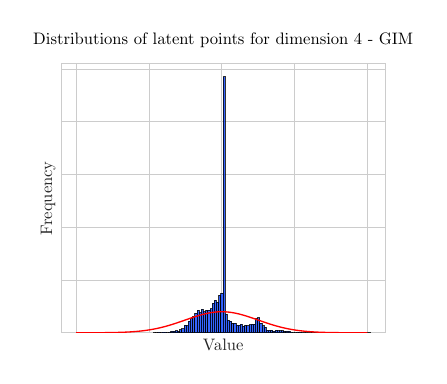
\begin{tikzpicture}[scale=0.6]

\definecolor{blue262255}{RGB}{2,62,255}
\definecolor{darkslategray38}{RGB}{38,38,38}
\definecolor{lightgray204}{RGB}{204,204,204}

\begin{axis}[
axis line style={lightgray204},
tick align=outside,
title={Distributions of latent points for dimension 4 - GIM},
x grid style={lightgray204},
xlabel=\textcolor{darkslategray38}{Value},
xmajorgrids,
xmajorticks=false,
xmin=-4.40414893627167, xmax=4.48712766170502,
xtick style={color=darkslategray38},
y grid style={lightgray204},
ylabel=\textcolor{darkslategray38}{Frequency},
ymajorgrids,
ymajorticks=false,
ymin=0, ymax=5.09827496196114,
ytick style={color=darkslategray38}
]
\draw[draw=black,fill=blue262255,opacity=0.8,line width=0.48pt] (axis cs:-1.87057781219482,0) rectangle (axis cs:-1.81104218959808,0.00446482364164092);
\draw[draw=black,fill=blue262255,opacity=0.8,line width=0.48pt] (axis cs:-1.81104218959808,0) rectangle (axis cs:-1.75150668621063,0.00446483258165863);
\draw[draw=black,fill=blue262255,opacity=0.8,line width=0.48pt] (axis cs:-1.75150656700134,0) rectangle (axis cs:-1.6919709444046,0.00669723546246138);
\draw[draw=black,fill=blue262255,opacity=0.8,line width=0.48pt] (axis cs:-1.69197106361389,0) rectangle (axis cs:-1.63243556022644,0.00223241629082931);
\draw[draw=black,fill=blue262255,opacity=0.8,line width=0.48pt] (axis cs:-1.63243556022644,0) rectangle (axis cs:-1.5728999376297,0.00669723546246138);
\draw[draw=black,fill=blue262255,opacity=0.8,line width=0.48pt] (axis cs:-1.5728999376297,0) rectangle (axis cs:-1.51336443424225,0.0111620814541466);
\draw[draw=black,fill=blue262255,opacity=0.8,line width=0.48pt] (axis cs:-1.51336431503296,0) rectangle (axis cs:-1.45382869243622,0.00223241182082046);
\draw[draw=black,fill=blue262255,opacity=0.8,line width=0.48pt] (axis cs:-1.45382881164551,0) rectangle (axis cs:-1.39429330825806,0.0133944977449759);
\draw[draw=black,fill=blue262255,opacity=0.8,line width=0.48pt] (axis cs:-1.39429330825806,0) rectangle (axis cs:-1.33475768566132,0.0312537654914865);
\draw[draw=black,fill=blue262255,opacity=0.8,line width=0.48pt] (axis cs:-1.33475768566132,0) rectangle (axis cs:-1.27522218227386,0.0312538280716104);
\draw[draw=black,fill=blue262255,opacity=0.8,line width=0.48pt] (axis cs:-1.27522206306458,0) rectangle (axis cs:-1.21568644046783,0.0379510009539478);
\draw[draw=black,fill=blue262255,opacity=0.8,line width=0.48pt] (axis cs:-1.21568655967712,0) rectangle (axis cs:-1.15615105628967,0.0334862443624397);
\draw[draw=black,fill=blue262255,opacity=0.8,line width=0.48pt] (axis cs:-1.15615105628967,0) rectangle (axis cs:-1.09661543369293,0.0558102955205115);
\draw[draw=black,fill=blue262255,opacity=0.8,line width=0.48pt] (axis cs:-1.09661543369293,0) rectangle (axis cs:-1.03707993030548,0.0803669864698553);
\draw[draw=black,fill=blue262255,opacity=0.8,line width=0.48pt] (axis cs:-1.03707981109619,0) rectangle (axis cs:-0.977544188499451,0.14287435653251);
\draw[draw=black,fill=blue262255,opacity=0.8,line width=0.48pt] (axis cs:-0.97754430770874,0) rectangle (axis cs:-0.918008804321289,0.133944843349359);
\draw[draw=black,fill=blue262255,opacity=0.8,line width=0.48pt] (axis cs:-0.918008685112,0) rectangle (axis cs:-0.858473181724548,0.216544163414797);
\draw[draw=black,fill=blue262255,opacity=0.8,line width=0.48pt] (axis cs:-0.858473181724548,0) rectangle (axis cs:-0.798937678337097,0.267889686698718);
\draw[draw=black,fill=blue262255,opacity=0.8,line width=0.48pt] (axis cs:-0.798937559127808,0) rectangle (axis cs:-0.739402055740356,0.312537967815171);
\draw[draw=black,fill=blue262255,opacity=0.8,line width=0.48pt] (axis cs:-0.739402055740356,0) rectangle (axis cs:-0.679866552352905,0.375045561378205);
\draw[draw=black,fill=blue262255,opacity=0.8,line width=0.48pt] (axis cs:-0.679866433143616,0) rectangle (axis cs:-0.620330929756165,0.428623498717949);
\draw[draw=black,fill=blue262255,opacity=0.8,line width=0.48pt] (axis cs:-0.620330929756165,0) rectangle (axis cs:-0.560795426368713,0.383975217601496);
\draw[draw=black,fill=blue262255,opacity=0.8,line width=0.48pt] (axis cs:-0.560795307159424,0) rectangle (axis cs:-0.501259803771973,0.450947639276175);
\draw[draw=black,fill=blue262255,opacity=0.8,line width=0.48pt] (axis cs:-0.501259803771973,0) rectangle (axis cs:-0.441724300384521,0.399602115992254);
\draw[draw=black,fill=blue262255,opacity=0.8,line width=0.48pt] (axis cs:-0.441724210977554,0) rectangle (axis cs:-0.382188707590103,0.426391084662126);
\draw[draw=black,fill=blue262255,opacity=0.8,line width=0.48pt] (axis cs:-0.382188647985458,0) rectangle (axis cs:-0.322653144598007,0.426391084662126);
\draw[draw=black,fill=blue262255,opacity=0.8,line width=0.48pt] (axis cs:-0.322653084993362,0) rectangle (axis cs:-0.263117581605911,0.457644881443643);
\draw[draw=black,fill=blue262255,opacity=0.8,line width=0.48pt] (axis cs:-0.263117522001266,0) rectangle (axis cs:-0.203582018613815,0.560335928011485);
\draw[draw=black,fill=blue262255,opacity=0.8,line width=0.48pt] (axis cs:-0.203582018613815,0) rectangle (axis cs:-0.144046396017075,0.622843365683);
\draw[draw=black,fill=blue262255,opacity=0.8,line width=0.48pt] (axis cs:-0.144046381115913,0) rectangle (axis cs:-0.0845108777284622,0.575962826402244);
\draw[draw=black,fill=blue262255,opacity=0.8,line width=0.48pt] (axis cs:-0.0845108181238174,0) rectangle (axis cs:-0.0249753147363663,0.712140083807425);
\draw[draw=black,fill=blue262255,opacity=0.8,line width=0.48pt] (axis cs:-0.0249752551317215,0) rectangle (axis cs:0.0345602482557297,0.752323536812233);
\draw[draw=black,fill=blue262255,opacity=0.8,line width=0.48pt] (axis cs:0.0345602482557297,0) rectangle (axis cs:0.0940958708524704,4.85549996377251);
\draw[draw=black,fill=blue262255,opacity=0.8,line width=0.48pt] (axis cs:0.0940958708524704,0) rectangle (axis cs:0.153631374239922,0.348256636290925);
\draw[draw=black,fill=blue262255,opacity=0.8,line width=0.48pt] (axis cs:0.153631389141083,0) rectangle (axis cs:0.213167011737823,0.23886824418667);
\draw[draw=black,fill=blue262255,opacity=0.8,line width=0.48pt] (axis cs:0.213167011737823,0) rectangle (axis cs:0.272702515125275,0.223241405582265);
\draw[draw=black,fill=blue262255,opacity=0.8,line width=0.48pt] (axis cs:0.272702574729919,0) rectangle (axis cs:0.332238078117371,0.18529036663328);
\draw[draw=black,fill=blue262255,opacity=0.8,line width=0.48pt] (axis cs:0.332238137722015,0) rectangle (axis cs:0.391773641109467,0.18529036663328);
\draw[draw=black,fill=blue262255,opacity=0.8,line width=0.48pt] (axis cs:0.391773700714111,0) rectangle (axis cs:0.451309204101562,0.140642085516827);
\draw[draw=black,fill=blue262255,opacity=0.8,line width=0.48pt] (axis cs:0.451309204101562,0) rectangle (axis cs:0.510844826698303,0.138409602175902);
\draw[draw=black,fill=blue262255,opacity=0.8,line width=0.48pt] (axis cs:0.510844826698303,0) rectangle (axis cs:0.570380330085754,0.167431054186699);
\draw[draw=black,fill=blue262255,opacity=0.8,line width=0.48pt] (axis cs:0.570380449295044,0) rectangle (axis cs:0.629915952682495,0.120550359014423);
\draw[draw=black,fill=blue262255,opacity=0.8,line width=0.48pt] (axis cs:0.629915952682495,0) rectangle (axis cs:0.689451456069946,0.147339327684295);
\draw[draw=black,fill=blue262255,opacity=0.8,line width=0.48pt] (axis cs:0.689451575279236,0) rectangle (axis cs:0.748987078666687,0.133944843349359);
\draw[draw=black,fill=blue262255,opacity=0.8,line width=0.48pt] (axis cs:0.748987078666687,0) rectangle (axis cs:0.808522582054138,0.154036569851763);
\draw[draw=black,fill=blue262255,opacity=0.8,line width=0.48pt] (axis cs:0.808522701263428,0) rectangle (axis cs:0.868058204650879,0.165198640130876);
\draw[draw=black,fill=blue262255,opacity=0.8,line width=0.48pt] (axis cs:0.868058204650879,0) rectangle (axis cs:0.92759370803833,0.165198640130876);
\draw[draw=black,fill=blue262255,opacity=0.8,line width=0.48pt] (axis cs:0.92759382724762,0) rectangle (axis cs:0.987129330635071,0.263424858587073);
\draw[draw=black,fill=blue262255,opacity=0.8,line width=0.48pt] (axis cs:0.987129330635071,0) rectangle (axis cs:1.04666483402252,0.285749285226152);
\draw[draw=black,fill=blue262255,opacity=0.8,line width=0.48pt] (axis cs:1.04666495323181,0) rectangle (axis cs:1.10620057582855,0.176360533844816);
\draw[draw=black,fill=blue262255,opacity=0.8,line width=0.48pt] (axis cs:1.10620045661926,0) rectangle (axis cs:1.165736079216,0.131712297428407);
\draw[draw=black,fill=blue262255,opacity=0.8,line width=0.48pt] (axis cs:1.165736079216,0) rectangle (axis cs:1.22527158260345,0.107155981959807);
\draw[draw=black,fill=blue262255,opacity=0.8,line width=0.48pt] (axis cs:1.22527170181274,0) rectangle (axis cs:1.28480732440948,0.0513454718788706);
\draw[draw=black,fill=blue262255,opacity=0.8,line width=0.48pt] (axis cs:1.2848072052002,0) rectangle (axis cs:1.34434270858765,0.0513455746890742);
\draw[draw=black,fill=blue262255,opacity=0.8,line width=0.48pt] (axis cs:1.34434270858765,0) rectangle (axis cs:1.40387833118439,0.0513454718788706);
\draw[draw=black,fill=blue262255,opacity=0.8,line width=0.48pt] (axis cs:1.40387833118439,0) rectangle (axis cs:1.46341383457184,0.0290214117807811);
\draw[draw=black,fill=blue262255,opacity=0.8,line width=0.48pt] (axis cs:1.46341395378113,0) rectangle (axis cs:1.52294957637787,0.0446482364164092);
\draw[draw=black,fill=blue262255,opacity=0.8,line width=0.48pt] (axis cs:1.52294945716858,0) rectangle (axis cs:1.58248496055603,0.042415909525757);
\draw[draw=black,fill=blue262255,opacity=0.8,line width=0.48pt] (axis cs:1.58248496055603,0) rectangle (axis cs:1.64202058315277,0.0424158245955888);
\draw[draw=black,fill=blue262255,opacity=0.8,line width=0.48pt] (axis cs:1.64202058315277,0) rectangle (axis cs:1.70155608654022,0.0379510769440983);
\draw[draw=black,fill=blue262255,opacity=0.8,line width=0.48pt] (axis cs:1.70155620574951,0) rectangle (axis cs:1.76109182834625,0.0312537654914865);
\draw[draw=black,fill=blue262255,opacity=0.8,line width=0.48pt] (axis cs:1.76109170913696,0) rectangle (axis cs:1.82062721252441,0.0290214117807811);
\draw[draw=black,fill=blue262255,opacity=0.8,line width=0.48pt] (axis cs:1.82062721252441,0) rectangle (axis cs:1.88016283512115,0.0245565300290251);
\draw[draw=black,fill=blue262255,opacity=0.8,line width=0.48pt] (axis cs:1.88016283512115,0) rectangle (axis cs:1.93969833850861,0.00892966516331725);
\draw[draw=black,fill=blue262255,opacity=0.8,line width=0.48pt] (axis cs:1.9396984577179,0) rectangle (axis cs:1.99923408031464,0.00446482364164092);
\draw[draw=black,fill=blue262255,opacity=0.8,line width=0.48pt] (axis cs:1.99923396110535,0) rectangle (axis cs:2.0587694644928,0.00446483258165863);
\draw[draw=black,fill=blue262255,opacity=0.8,line width=0.48pt] (axis cs:2.0587694644928,0) rectangle (axis cs:2.11830496788025,0.00892966516331725);
\draw[draw=black,fill=blue262255,opacity=0.8,line width=0.48pt] (axis cs:2.11830472946167,0) rectangle (axis cs:2.1778404712677,0.00892962940331804);
\draw[draw=black,fill=blue262255,opacity=0.8,line width=0.48pt] (axis cs:2.17784070968628,0) rectangle (axis cs:2.23737621307373,0);
\draw[draw=black,fill=blue262255,opacity=0.8,line width=0.48pt] (axis cs:2.23737621307373,0) rectangle (axis cs:2.29691171646118,0.00446483258165863);
\draw[draw=black,fill=blue262255,opacity=0.8,line width=0.48pt] (axis cs:2.29691171646118,0) rectangle (axis cs:2.35644721984863,0);
\draw[draw=black,fill=blue262255,opacity=0.8,line width=0.48pt] (axis cs:2.35644721984863,0) rectangle (axis cs:2.41598296165466,0.00446481470165902);
\draw[draw=black,fill=blue262255,opacity=0.8,line width=0.48pt] (axis cs:2.41598296165466,0) rectangle (axis cs:2.47551846504211,0);
\draw[draw=black,fill=blue262255,opacity=0.8,line width=0.48pt] (axis cs:2.47551846504211,0) rectangle (axis cs:2.53505396842957,0.00223241629082931);
\draw[draw=black,fill=blue262255,opacity=0.8,line width=0.48pt] (axis cs:2.53505373001099,0) rectangle (axis cs:2.59458947181702,0);
\draw[draw=black,fill=blue262255,opacity=0.8,line width=0.48pt] (axis cs:2.5945897102356,0) rectangle (axis cs:2.65412521362305,0);
\draw[draw=black,fill=blue262255,opacity=0.8,line width=0.48pt] (axis cs:2.65412521362305,0) rectangle (axis cs:2.7136607170105,0);
\draw[draw=black,fill=blue262255,opacity=0.8,line width=0.48pt] (axis cs:2.7136607170105,0) rectangle (axis cs:2.77319622039795,0);
\draw[draw=black,fill=blue262255,opacity=0.8,line width=0.48pt] (axis cs:2.77319622039795,0) rectangle (axis cs:2.83273196220398,0);
\draw[draw=black,fill=blue262255,opacity=0.8,line width=0.48pt] (axis cs:2.83273196220398,0) rectangle (axis cs:2.89226746559143,0.00223241629082931);
\draw[draw=black,fill=blue262255,opacity=0.8,line width=0.48pt] (axis cs:2.89226746559143,0) rectangle (axis cs:2.95180296897888,0.00223241629082931);
\draw[draw=black,fill=blue262255,opacity=0.8,line width=0.48pt] (axis cs:2.95180296897888,0) rectangle (axis cs:3.01133847236633,0);
\draw[draw=black,fill=blue262255,opacity=0.8,line width=0.48pt] (axis cs:3.01133823394775,0) rectangle (axis cs:3.07087397575378,0);
\draw[draw=black,fill=blue262255,opacity=0.8,line width=0.48pt] (axis cs:3.07087421417236,0) rectangle (axis cs:3.13040971755981,0);
\draw[draw=black,fill=blue262255,opacity=0.8,line width=0.48pt] (axis cs:3.13040971755981,0) rectangle (axis cs:3.18994522094727,0);
\draw[draw=black,fill=blue262255,opacity=0.8,line width=0.48pt] (axis cs:3.18994522094727,0) rectangle (axis cs:3.24948072433472,0.00223241629082931);
\draw[draw=black,fill=blue262255,opacity=0.8,line width=0.48pt] (axis cs:3.24948072433472,0) rectangle (axis cs:3.30901646614075,0);
\draw[draw=black,fill=blue262255,opacity=0.8,line width=0.48pt] (axis cs:3.30901646614075,0) rectangle (axis cs:3.3685519695282,0);
\draw[draw=black,fill=blue262255,opacity=0.8,line width=0.48pt] (axis cs:3.3685519695282,0) rectangle (axis cs:3.42808747291565,0.00223241629082931);
\draw[draw=black,fill=blue262255,opacity=0.8,line width=0.48pt] (axis cs:3.42808747291565,0) rectangle (axis cs:3.4876229763031,0);
\draw[draw=black,fill=blue262255,opacity=0.8,line width=0.48pt] (axis cs:3.48762273788452,0) rectangle (axis cs:3.54715847969055,0);
\draw[draw=black,fill=blue262255,opacity=0.8,line width=0.48pt] (axis cs:3.54715871810913,0) rectangle (axis cs:3.60669422149658,0);
\draw[draw=black,fill=blue262255,opacity=0.8,line width=0.48pt] (axis cs:3.60669422149658,0) rectangle (axis cs:3.66622972488403,0);
\draw[draw=black,fill=blue262255,opacity=0.8,line width=0.48pt] (axis cs:3.66622972488403,0) rectangle (axis cs:3.72576522827148,0);
\draw[draw=black,fill=blue262255,opacity=0.8,line width=0.48pt] (axis cs:3.72576522827148,0) rectangle (axis cs:3.78530097007751,0.00223240735082951);
\draw[draw=black,fill=blue262255,opacity=0.8,line width=0.48pt] (axis cs:3.78530097007751,0) rectangle (axis cs:3.84483647346497,0);
\draw[draw=black,fill=blue262255,opacity=0.8,line width=0.48pt] (axis cs:3.84483647346497,0) rectangle (axis cs:3.90437197685242,0);
\draw[draw=black,fill=blue262255,opacity=0.8,line width=0.48pt] (axis cs:3.90437197685242,0) rectangle (axis cs:3.96390748023987,0);
\draw[draw=black,fill=blue262255,opacity=0.8,line width=0.48pt] (axis cs:3.96390724182129,0) rectangle (axis cs:4.0234432220459,0);
\draw[draw=black,fill=blue262255,opacity=0.8,line width=0.48pt] (axis cs:4.0234432220459,0) rectangle (axis cs:4.08297872543335,0.00223241629082931);
\addplot [thick, red]
table {%
-4 0.000133830225764885
-3.99199199199199 0.000138182046410498
-3.98398398398398 0.000142666228042307
-3.97597597597598 0.000147286481503254
-3.96796796796797 0.000152046611333821
-3.95995995995996 0.000156950517814782
-3.95195195195195 0.00016200219904485
-3.94394394394394 0.00016720575305353
-3.93593593593594 0.000172565379949496
-3.92792792792793 0.00017808538410479
-3.91991991991992 0.000183770176375138
-3.91191191191191 0.000189624276356684
-3.9039039039039 0.000195652314679408
-3.8958958958959 0.000201859035337517
-3.88788788788789 0.000208249298057069
-3.87987987987988 0.000214828080701088
-3.87187187187187 0.000221600481712426
-3.86386386386386 0.0002285717225946
-3.85585585585586 0.000235747150430845
-3.84784784784785 0.000243132240441603
-3.83983983983984 0.000250732598580649
-3.83183183183183 0.000258553964170059
-3.82382382382382 0.000266602212574213
-3.81581581581582 0.000274883357912987
-3.80780780780781 0.000283403555814325
-3.7997997997998 0.000292169106206322
-3.79179179179179 0.000301186456148957
-3.78378378378378 0.0003104622027056
-3.77577577577578 0.000320003095854415
-3.76776776776777 0.000329816041439723
-3.75975975975976 0.000339908104163431
-3.75175175175175 0.00035028651061658
-3.74374374374374 0.000360958652351047
-3.73573573573574 0.000371932088991451
-3.72772772772773 0.000383214551387261
-3.71971971971972 0.000394813944805093
-3.71171171171171 0.000406738352161197
-3.7037037037037 0.000418996037294058
-3.6956956956957 0.00043159544827708
-3.68768768768769 0.00044454522077123
-3.67967967967968 0.000457854181417586
-3.67167167167167 0.000471531351269624
-3.66366366366366 0.000485585949265103
-3.65565565565566 0.000500027395737409
-3.64764764764765 0.000514865315966112
-3.63963963963964 0.000530109543766577
-3.63163163163163 0.000545770125118336
-3.62362362362362 0.000561857321831991
-3.61561561561562 0.00057838161525435
-3.60760760760761 0.000595353710011453
-3.5995995995996 0.000612784537789192
-3.59159159159159 0.000630685261151105
-3.58358358358358 0.000649067277392973
-3.57557557557558 0.000667942222433796
-3.56756756756757 0.000687321974742665
-3.55955955955956 0.000707218659301081
-3.55155155155155 0.000727644651600166
-3.54354354354354 0.000748612581672245
-3.53553553553554 0.000770135338156225
-3.52752752752753 0.000792226072396121
-3.51951951951952 0.00081489820257214
-3.51151151151151 0.000838165417863603
-3.5035035035035 0.000862041682643007
-3.4954954954955 0.000886541240700502
-3.48748748748749 0.00091167861949796
-3.47947947947948 0.000937468634451866
-3.47147147147147 0.000963926393244149
-3.46346346346346 0.000991067300160059
-3.45545545545546 0.0010189070604522
-3.44744744744745 0.00104746168472971
-3.43943943943944 0.0010767474933716
-3.43143143143143 0.00110678112096323
-3.42342342342342 0.00113757952075483
-3.41541541541542 0.00116915996914087
-3.40740740740741 0.00120154007015926
-3.3993993993994 0.00123473776000907
-3.39139139139139 0.00126877131158549
-3.38338338338338 0.00130365933903088
-3.37537537537538 0.00133942080230046
-3.36736736736737 0.00137607501174126
-3.35935935935936 0.001413641632683
-3.35135135135135 0.00145214069003938
-3.34334334334334 0.0014915925729182
-3.33533533533534 0.00153201803923895
-3.32732732732733 0.00157343822035606
-3.31931931931932 0.00161587462568624
-3.31131131131131 0.00165934914733831
-3.3033033033033 0.00170388406474362
-3.2952952952953 0.00174950204928538
-3.28728728728729 0.00179622616892505
-3.27927927927928 0.00184407989282385
-3.27127127127127 0.00189308709595757
-3.26326326326326 0.00194327206372255
-3.25525525525526 0.00199465949653091
-3.24724724724725 0.00204727451439301
-3.23923923923924 0.00210114266148476
-3.23123123123123 0.00215628991069791
-3.22322322322322 0.00221274266817093
-3.21521521521522 0.00227052777779815
-3.20720720720721 0.00232967252571501
-3.1991991991992 0.00239020464475689
-3.19119119119119 0.00245215231888918
-3.18318318318318 0.00251554418760605
-3.17517517517518 0.00258040935029545
-3.16716716716717 0.00264677737056774
-3.15915915915916 0.00271467828054534
-3.15115115115115 0.00278414258511061
-3.14314314314314 0.00285520126610952
-3.13513513513514 0.00292788578650791
-3.12712712712713 0.00300222809449793
-3.11911911911912 0.00307826062755151
-3.11111111111111 0.00315601631641804
-3.1031031031031 0.00323552858906328
-3.0950950950951 0.00331683137454643
-3.08708708708709 0.00339995910683238
-3.07907907907908 0.00348494672853595
-3.07107107107107 0.00357182969459489
-3.06306306306306 0.00366064397586864
-3.05505505505506 0.00375142606265932
-3.04704704704705 0.00384421296815189
-3.03903903903904 0.00393904223176991
-3.03103103103103 0.00403595192244368
-3.02302302302302 0.0041349806417872
-3.01501501501502 0.00423616752718052
-3.00700700700701 0.00433955225475399
-2.998998998999 0.00444517504227068
-2.99099099099099 0.00455307665190355
-2.98298298298298 0.00466329839290368
-2.97497497497497 0.00477588212415564
-2.96696696696697 0.00489087025661667
-2.95895895895896 0.00500830575563558
-2.95095095095095 0.00512823214314763
-2.94294294294294 0.00525069349974172
-2.93493493493493 0.00537573446659573
-2.92692692692693 0.00550340024727644
-2.91891891891892 0.00563373660939975
-2.91091091091091 0.0057667898861475
-2.9029029029029 0.00590260697763674
-2.89489489489489 0.00604123535213746
-2.88688688688689 0.00618272304713484
-2.87887887887888 0.00632711867023164
-2.87087087087087 0.00647447139988703
-2.86286286286286 0.00662483098598741
-2.85485485485485 0.0067782477502453
-2.84684684684685 0.0069347725864219
-2.83883883883884 0.00709445696036946
-2.83083083083083 0.00725735290988893
-2.82282282282282 0.00742351304439893
-2.81481481481481 0.00759299054441176
-2.80680680680681 0.0077658391608121
-2.7987987987988 0.00794211321393437
-2.79079079079079 0.00812186759243432
-2.78278278278278 0.00830515775195071
-2.77477477477477 0.00849203971355293
-2.76676676676677 0.00868257006197001
-2.75875875875876 0.00887680594359712
-2.75075075075075 0.00907480506427511
-2.74274274274274 0.00927662568683898
-2.73473473473473 0.00948232662843099
-2.72672672672673 0.00969196725757422
-2.71871871871872 0.00990560749100246
-2.71071071071071 0.0101233077902421
-2.7027027027027 0.0103451291579421
-2.69469469469469 0.0105711331339476
-2.68668668668669 0.0108013817911136
-2.67867867867868 0.011035937730854
-2.67067067067067 0.0112748640784219
-2.66266266266266 0.0115182244779185
-2.65465465465465 0.0117660830870247
-2.64664664664665 0.0120185045714526
-2.63863863863864 0.0122755540991133
-2.63063063063063 0.0125372973339956
-2.62262262262262 0.0128038004297541
-2.61461461461461 0.0130751300230007
-2.60660660660661 0.0133513532262973
-2.5985985985986 0.0136325376208454
-2.59059059059059 0.0139187512488692
-2.58258258258258 0.014210062605689
-2.57457457457457 0.0145065406314803
-2.56656656656657 0.0148082547027168
-2.55855855855856 0.0151152746232934
-2.55055055055055 0.0154276706153247
-2.54254254254254 0.0157455133096184
-2.53453453453453 0.0160688737358178
-2.52652652652653 0.016397823312213
-2.51851851851852 0.0167324338352151
-2.51051051051051 0.0170727774684938
-2.5025025025025 0.0174189267317727
-2.49449449449449 0.0177709544892815
-2.48648648648649 0.0181289339378627
-2.47847847847848 0.0184929385947284
-2.47047047047047 0.0188630422848682
-2.46246246246246 0.0192393191281025
-2.45445445445445 0.0196218435257817
-2.44644644644645 0.0200106901471285
-2.43843843843844 0.020405933915221
-2.43043043043043 0.0208076499926159
-2.42242242242242 0.0212159137666093
-2.41441441441441 0.0216308008341344
-2.40640640640641 0.0220523869862944
-2.3983983983984 0.0224807481925294
-2.39039039039039 0.022915960584417
-2.38238238238238 0.0233581004391047
-2.37437437437437 0.023807244162374
-2.36636636636637 0.0242634682713357
-2.35835835835836 0.0247268493767558
-2.35035035035035 0.0251974641650118
-2.34234234234234 0.0256753893796796
-2.33433433433433 0.0261607018027501
-2.32632632632633 0.0266534782354775
-2.31831831831832 0.0271537954788581
-2.31031031031031 0.0276617303137407
-2.3023023023023 0.0281773594805703
-2.29429429429429 0.0287007596587648
-2.28628628628629 0.0292320074457259
-2.27827827827828 0.029771179335487
-2.27027027027027 0.0303183516969979
-2.26226226226226 0.0308736007520491
-2.25425425425425 0.0314370025528369
-2.24624624624625 0.0320086329591723
-2.23823823823824 0.0325885676153351
-2.23023023023023 0.0331768819265761
-2.22222222222222 0.0337736510352706
-2.21421421421421 0.0343789497967251
-2.20620620620621 0.0349928527546413
-2.1981981981982 0.0356154341162401
-2.19019019019019 0.0362467677270497
-2.18218218218218 0.0368869270453615
-2.17417417417417 0.0375359851163567
-2.16616616616617 0.03819401454591
-2.15815815815816 0.0388610874740724
-2.15015015015015 0.03953727554824
-2.14214214214214 0.0402226498960119
-2.13413413413413 0.0409172810977437
-2.12612612612613 0.0416212391588003
-2.11811811811812 0.0423345934815158
-2.11011011011011 0.0430574128368641
-2.1021021021021 0.043789765335848
-2.09409409409409 0.0445317184006117
-2.08608608608609 0.0452833387352837
-2.07807807807808 0.0460446922965577
-2.07007007007007 0.0468158442640166
-2.06206206206206 0.0475968590102091
-2.05405405405405 0.0483878000704834
-2.04604604604605 0.0491887301125894
-2.03803803803804 0.0499997109060533
-2.03003003003003 0.0508208032913361
-2.02202202202202 0.0516520671487823
-2.01401401401401 0.0524935613673682
-2.00600600600601 0.053345343813258
-1.997997997998 0.0542074712981785
-1.98998998998999 0.0550799995476186
-1.98198198198198 0.0559629831688668
-1.97397397397397 0.0568564756188931
-1.96596596596597 0.0577605291720876
-1.95795795795796 0.0586751948878651
-1.94994994994995 0.0596005225781457
-1.94194194194194 0.0605365607747232
-1.93393393393393 0.0614833566965309
-1.92592592592593 0.062440956216817
-1.91791791791792 0.06340940383024
-1.90990990990991 0.0643887426198963
-1.9019019019019 0.0653790142242912
-1.89389389389389 0.0663802588042656
-1.88588588588589 0.0673925150098903
-1.87787787787788 0.0684158199473405
-1.86986986986987 0.0694502091457625
-1.86186186186186 0.0704957165241465
-1.85385385385385 0.0715523743582165
-1.84584584584585 0.0726202132473521
-1.83783783783784 0.0736992620815557
-1.82982982982983 0.0747895480084762
-1.82182182182182 0.0758910964005057
-1.81381381381381 0.0770039308219614
-1.80580580580581 0.0781280729963669
-1.7977977977978 0.0792635427738473
-1.78978978978979 0.0804103580986525
-1.78178178178178 0.0815685349768227
-1.77377377377377 0.0827380874440109
-1.76576576576577 0.0839190275334777
-1.75775775775776 0.0851113652442723
-1.74974974974975 0.086315108509615
-1.74174174174174 0.0875302631654975
-1.73373373373373 0.0887568329195139
-1.72572572572573 0.0899948193199405
-1.71771771771772 0.0912442217250772
-1.70970970970971 0.0925050372728685
-1.7017017017017 0.0937772608508177
-1.69369369369369 0.0950608850662112
-1.68568568568569 0.0963559002166691
-1.67767767767768 0.0976622942610365
-1.66966966966967 0.0989800527906321
-1.66166166166166 0.100309159000872
-1.65365365365365 0.10164959366328
-1.64564564564565 0.103001335097907
-1.63763763763764 0.10436435914617
-1.62962962962963 0.105738639144131
-1.62162162162162 0.107124145896225
-1.61361361361361 0.108520847649465
-1.60560560560561 0.10992871006813
-1.5975975975976 0.111347696208955
-1.58958958958959 0.112777766496842
-1.58158158158158 0.114218878701105
-1.57357357357357 0.115670987912262
-1.56556556556557 0.117134046519405
-1.55755755755756 0.11860800418814
-1.54954954954955 0.120092807839133
-1.54154154154154 0.121588401627275
-1.53353353353353 0.123094726921466
-1.52552552552553 0.124611722285057
-1.51751751751752 0.12613932345695
-1.50950950950951 0.127677463333369
-1.5015015015015 0.129226071950339
-1.49349349349349 0.130785076466857
-1.48548548548549 0.132354401148798
-1.47747747747748 0.133933967353555
-1.46946946946947 0.13552369351543
-1.46146146146146 0.137123495131801
-1.45345345345345 0.13873328475006
-1.44544544544545 0.140352971955359
-1.43743743743744 0.141982463359159
-1.42942942942943 0.143621662588612
-1.42142142142142 0.14527047027677
-1.41341341341341 0.146928784053658
-1.40540540540541 0.148596498538208
-1.3973973973974 0.150273505331067
-1.38938938938939 0.151959693008306
-1.38138138138138 0.153654947116025
-1.37337337337337 0.155359150165875
-1.36536536536537 0.157072181631514
-1.35735735735736 0.158793917945997
-1.34934934934935 0.160524232500121
-1.34134134134134 0.16226299564173
-1.33333333333333 0.164010074675994
-1.32532532532533 0.165765333866673
-1.31731731731732 0.167528634438376
-1.30930930930931 0.169299834579821
-1.3013013013013 0.17107878944811
-1.29329329329329 0.172865351174024
-1.28528528528529 0.174659368868355
-1.27727727727728 0.176460688629273
-1.26926926926927 0.178269153550739
-1.26126126126126 0.180084603731981
-1.25325325325325 0.181906876288021
-1.24524524524525 0.183735805361283
-1.23723723723724 0.185571222134271
-1.22922922922923 0.187412954843324
-1.22122122122122 0.18926082879347
-1.21321321321321 0.191114666374361
-1.20520520520521 0.192974287077311
-1.1971971971972 0.194839507513435
-1.18918918918919 0.19671014143289
-1.18118118118118 0.198585999745227
-1.17317317317317 0.200466890540856
-1.16516516516517 0.202352619113618
-1.15715715715716 0.204242987984477
-1.14914914914915 0.206137796926331
-1.14114114114114 0.208036842989938
-1.13313313313313 0.209939920530956
-1.12512512512513 0.21184682123811
-1.11711711711712 0.21375733416247
-1.10910910910911 0.215671245747847
-1.1011011011011 0.217588339862305
-1.09309309309309 0.219508397830784
-1.08508508508509 0.221431198468836
-1.07707707707708 0.223356518117463
-1.06906906906907 0.225284130679063
-1.06106106106106 0.22721380765447
-1.05305305305305 0.229145318181096
-1.04504504504505 0.231078429072154
-1.03703703703704 0.233012904856966
-1.02902902902903 0.234948507822352
-1.02102102102102 0.236884998055083
-1.01301301301301 0.238822133485401
-1.00500500500501 0.24075966993159
-0.996996996996997 0.242697361145593
-0.988988988988989 0.244634958859672
-0.980980980980981 0.246572212834085
-0.972972972972973 0.248508870905785
-0.964964964964965 0.250444679038131
-0.956956956956957 0.252379381371581
-0.948948948948949 0.254312720275385
-0.940940940940941 0.256244436400228
-0.932932932932933 0.258174268731856
-0.924924924924925 0.260101954645624
-0.916916916916917 0.262027229961987
-0.908908908908909 0.263949829002911
-0.900900900900901 0.265869484649172
-0.892892892892893 0.267785928398552
-0.884884884884885 0.269698890424904
-0.876876876876877 0.271608099638066
-0.868868868868869 0.273513283744617
-0.860860860860861 0.275414169309444
-0.852852852852853 0.277310481818125
-0.844844844844845 0.279201945740075
-0.836836836836837 0.281088284592474
-0.828828828828829 0.28296922100493
-0.820820820820821 0.284844476784867
-0.812812812812813 0.286713772983616
-0.804804804804805 0.288576829963198
-0.796796796796797 0.290433367463758
-0.788788788788789 0.292283104671645
-0.780780780780781 0.294125760288111
-0.772772772772773 0.295961052598604
-0.764764764764765 0.29778869954263
-0.756756756756757 0.299608418784177
-0.748748748748749 0.301419927782648
-0.740740740740741 0.303222943864308
-0.732732732732733 0.305017184294205
-0.724724724724725 0.306802366348536
-0.716716716716717 0.308578207387456
-0.708708708708709 0.310344424928268
-0.700700700700701 0.312100736719007
-0.692692692692693 0.313846860812361
-0.684684684684685 0.31558251563992
-0.676676676676677 0.317307420086723
-0.668668668668669 0.319021293566066
-0.660660660660661 0.320723856094559
-0.652652652652653 0.322414828367396
-0.644644644644645 0.324093931833804
-0.636636636636636 0.325760888772662
-0.628628628628629 0.327415422368237
-0.620620620620621 0.329057256786028
-0.612612612612613 0.330686117248681
-0.604604604604605 0.33230173011195
-0.596596596596596 0.333903822940662
-0.588588588588589 0.335492124584683
-0.580580580580581 0.337066365254824
-0.572572572572573 0.338626276598684
-0.564564564564565 0.340171591776383
-0.556556556556556 0.341702045536168
-0.548548548548549 0.343217374289848
-0.54054054054054 0.344717316188045
-0.532532532532533 0.346201611195215
-0.524524524524525 0.347670001164422
-0.516516516516516 0.349122229911825
-0.508508508508509 0.350558043290856
-0.5005005005005 0.351977189266054
-0.492492492492492 0.353379417986526
-0.484484484484485 0.354764481859011
-0.476476476476476 0.356132135620502
-0.468468468468469 0.357482136410418
-0.46046046046046 0.358814243842273
-0.452452452452452 0.360128220074839
-0.444444444444445 0.361423829882744
-0.436436436436436 0.362700840726495
-0.428428428428429 0.363959022821904
-0.42042042042042 0.365198149208855
-0.412412412412412 0.366417995819425
-0.404404404404405 0.3676183415453
-0.396396396396396 0.368798968304465
-0.388388388388389 0.369959661107154
-0.38038038038038 0.37110020812101
-0.372372372372372 0.372220400735444
-0.364364364364365 0.373320033625156
-0.356356356356356 0.374398904812801
-0.348348348348348 0.375456815730761
-0.34034034034034 0.376493571282005
-0.332332332332332 0.377508979900006
-0.324324324324325 0.378502853607702
-0.316316316316316 0.379475008075448
-0.308308308308308 0.380425262677969
-0.3003003003003 0.38135344055026
-0.292292292292292 0.382259368642425
-0.284284284284285 0.38314287777343
-0.276276276276276 0.384003802683735
-0.268268268268268 0.3848419820868
-0.26026026026026 0.385657258719425
-0.252252252252252 0.386449479390916
-0.244244244244244 0.387218495031049
-0.236236236236236 0.387964160736805
-0.228228228228228 0.38868633581787
-0.22022022022022 0.389384883840873
-0.212212212212212 0.390059672672329
-0.204204204204204 0.390710574520297
-0.196196196196196 0.391337465974705
-0.188188188188188 0.39194022804635
-0.18018018018018 0.392518746204527
-0.172172172172172 0.393072910413305
-0.164164164164164 0.393602615166401
-0.156156156156156 0.394107759520658
-0.148148148148148 0.394588247128102
-0.14014014014014 0.395043986266573
-0.132132132132132 0.3954748898689
-0.124124124124124 0.395880875550626
-0.116116116116116 0.396261865636259
-0.108108108108108 0.396617787184037
-0.1001001001001 0.396948572009207
-0.0920920920920922 0.397254156705792
-0.084084084084084 0.397534482666846
-0.0760760760760761 0.39778949610319
-0.0680680680680683 0.39801914806061
-0.06006006006006 0.398223394435522
-0.0520520520520522 0.398402195989086
-0.0440440440440439 0.398555518359772
-0.0360360360360361 0.398683332074364
-0.0280280280280278 0.398785612557403
-0.02002002002002 0.398862340139061
-0.0120120120120122 0.398913500061449
-0.00400400400400391 0.398939082483343
0.00400400400400436 0.398939082483343
0.0120120120120122 0.398913500061449
0.02002002002002 0.398862340139061
0.0280280280280278 0.398785612557403
0.0360360360360357 0.398683332074364
0.0440440440440444 0.398555518359772
0.0520520520520522 0.398402195989086
0.06006006006006 0.398223394435522
0.0680680680680679 0.39801914806061
0.0760760760760757 0.39778949610319
0.0840840840840844 0.397534482666846
0.0920920920920922 0.397254156705792
0.1001001001001 0.396948572009207
0.108108108108108 0.396617787184037
0.116116116116116 0.396261865636259
0.124124124124124 0.395880875550626
0.132132132132132 0.3954748898689
0.14014014014014 0.395043986266573
0.148148148148148 0.394588247128102
0.156156156156156 0.394107759520658
0.164164164164164 0.393602615166401
0.172172172172172 0.393072910413305
0.18018018018018 0.392518746204527
0.188188188188188 0.39194022804635
0.196196196196196 0.391337465974705
0.204204204204204 0.390710574520297
0.212212212212212 0.390059672672329
0.22022022022022 0.389384883840873
0.228228228228228 0.388686335817871
0.236236236236236 0.387964160736805
0.244244244244245 0.387218495031049
0.252252252252252 0.386449479390916
0.26026026026026 0.385657258719425
0.268268268268268 0.3848419820868
0.276276276276276 0.384003802683735
0.284284284284285 0.38314287777343
0.292292292292292 0.382259368642425
0.3003003003003 0.38135344055026
0.308308308308308 0.380425262677969
0.316316316316316 0.379475008075448
0.324324324324325 0.378502853607702
0.332332332332332 0.377508979900006
0.34034034034034 0.376493571282005
0.348348348348348 0.375456815730762
0.356356356356356 0.374398904812801
0.364364364364365 0.373320033625156
0.372372372372372 0.372220400735444
0.38038038038038 0.37110020812101
0.388388388388388 0.369959661107154
0.396396396396397 0.368798968304465
0.404404404404405 0.3676183415453
0.412412412412412 0.366417995819425
0.42042042042042 0.365198149208855
0.428428428428428 0.363959022821904
0.436436436436437 0.362700840726495
0.444444444444445 0.361423829882744
0.452452452452452 0.360128220074839
0.46046046046046 0.358814243842273
0.468468468468468 0.357482136410418
0.476476476476477 0.356132135620502
0.484484484484485 0.354764481859011
0.492492492492492 0.353379417986526
0.5005005005005 0.351977189266054
0.508508508508508 0.350558043290856
0.516516516516517 0.349122229911825
0.524524524524525 0.347670001164422
0.532532532532533 0.346201611195215
0.54054054054054 0.344717316188045
0.548548548548548 0.343217374289848
0.556556556556557 0.341702045536168
0.564564564564565 0.340171591776383
0.572572572572573 0.338626276598684
0.58058058058058 0.337066365254824
0.588588588588588 0.335492124584683
0.596596596596597 0.333903822940662
0.604604604604605 0.33230173011195
0.612612612612613 0.330686117248681
0.62062062062062 0.329057256786028
0.628628628628628 0.327415422368237
0.636636636636637 0.325760888772662
0.644644644644645 0.324093931833804
0.652652652652653 0.322414828367396
0.66066066066066 0.32072385609456
0.668668668668668 0.319021293566066
0.676676676676677 0.317307420086723
0.684684684684685 0.31558251563992
0.692692692692693 0.313846860812361
0.7007007007007 0.312100736719007
0.708708708708708 0.310344424928268
0.716716716716717 0.308578207387456
0.724724724724725 0.306802366348536
0.732732732732733 0.305017184294205
0.74074074074074 0.303222943864308
0.748748748748748 0.301419927782648
0.756756756756757 0.299608418784177
0.764764764764765 0.29778869954263
0.772772772772773 0.295961052598604
0.780780780780781 0.294125760288111
0.788788788788788 0.292283104671645
0.796796796796797 0.290433367463758
0.804804804804805 0.288576829963198
0.812812812812813 0.286713772983616
0.820820820820821 0.284844476784867
0.828828828828828 0.282969221004931
0.836836836836837 0.281088284592474
0.844844844844845 0.279201945740075
0.852852852852853 0.277310481818125
0.860860860860861 0.275414169309444
0.868868868868869 0.273513283744617
0.876876876876877 0.271608099638066
0.884884884884885 0.269698890424904
0.892892892892893 0.267785928398552
0.900900900900901 0.265869484649172
0.908908908908909 0.263949829002911
0.916916916916917 0.262027229961987
0.924924924924925 0.260101954645624
0.932932932932933 0.258174268731856
0.940940940940941 0.256244436400228
0.948948948948949 0.254312720275384
0.956956956956957 0.252379381371581
0.964964964964965 0.250444679038131
0.972972972972973 0.248508870905785
0.980980980980981 0.246572212834085
0.988988988988989 0.244634958859672
0.996996996996997 0.242697361145593
1.00500500500501 0.24075966993159
1.01301301301301 0.238822133485401
1.02102102102102 0.236884998055083
1.02902902902903 0.234948507822352
1.03703703703704 0.233012904856966
1.04504504504505 0.231078429072154
1.05305305305305 0.229145318181096
1.06106106106106 0.22721380765447
1.06906906906907 0.225284130679062
1.07707707707708 0.223356518117463
1.08508508508509 0.221431198468836
1.09309309309309 0.219508397830784
1.1011011011011 0.217588339862305
1.10910910910911 0.215671245747847
1.11711711711712 0.21375733416247
1.12512512512513 0.21184682123811
1.13313313313313 0.209939920530956
1.14114114114114 0.208036842989938
1.14914914914915 0.206137796926331
1.15715715715716 0.204242987984477
1.16516516516517 0.202352619113618
1.17317317317317 0.200466890540856
1.18118118118118 0.198585999745228
1.18918918918919 0.19671014143289
1.1971971971972 0.194839507513435
1.20520520520521 0.192974287077311
1.21321321321321 0.191114666374361
1.22122122122122 0.18926082879347
1.22922922922923 0.187412954843324
1.23723723723724 0.185571222134271
1.24524524524525 0.183735805361283
1.25325325325325 0.181906876288021
1.26126126126126 0.180084603731981
1.26926926926927 0.178269153550739
1.27727727727728 0.176460688629273
1.28528528528529 0.174659368868355
1.29329329329329 0.172865351174024
1.3013013013013 0.17107878944811
1.30930930930931 0.169299834579821
1.31731731731732 0.167528634438376
1.32532532532533 0.165765333866673
1.33333333333333 0.164010074675994
1.34134134134134 0.16226299564173
1.34934934934935 0.160524232500121
1.35735735735736 0.158793917945997
1.36536536536537 0.157072181631514
1.37337337337337 0.155359150165875
1.38138138138138 0.153654947116025
1.38938938938939 0.151959693008306
1.3973973973974 0.150273505331067
1.40540540540541 0.148596498538208
1.41341341341341 0.146928784053658
1.42142142142142 0.14527047027677
1.42942942942943 0.143621662588612
1.43743743743744 0.141982463359159
1.44544544544545 0.140352971955359
1.45345345345345 0.13873328475006
1.46146146146146 0.137123495131801
1.46946946946947 0.13552369351543
1.47747747747748 0.133933967353555
1.48548548548549 0.132354401148798
1.49349349349349 0.130785076466857
1.5015015015015 0.129226071950339
1.50950950950951 0.127677463333369
1.51751751751752 0.12613932345695
1.52552552552553 0.124611722285057
1.53353353353353 0.123094726921466
1.54154154154154 0.121588401627275
1.54954954954955 0.120092807839133
1.55755755755756 0.11860800418814
1.56556556556557 0.117134046519405
1.57357357357357 0.115670987912262
1.58158158158158 0.114218878701105
1.58958958958959 0.112777766496842
1.5975975975976 0.111347696208955
1.60560560560561 0.10992871006813
1.61361361361361 0.108520847649465
1.62162162162162 0.107124145896225
1.62962962962963 0.105738639144131
1.63763763763764 0.10436435914617
1.64564564564565 0.103001335097907
1.65365365365365 0.10164959366328
1.66166166166166 0.100309159000872
1.66966966966967 0.0989800527906321
1.67767767767768 0.0976622942610365
1.68568568568569 0.0963559002166692
1.69369369369369 0.0950608850662112
1.7017017017017 0.0937772608508176
1.70970970970971 0.0925050372728685
1.71771771771772 0.0912442217250772
1.72572572572573 0.0899948193199405
1.73373373373373 0.088756832919514
1.74174174174174 0.0875302631654974
1.74974974974975 0.086315108509615
1.75775775775776 0.0851113652442723
1.76576576576577 0.0839190275334778
1.77377377377377 0.082738087444011
1.78178178178178 0.0815685349768226
1.78978978978979 0.0804103580986525
1.7977977977978 0.0792635427738473
1.80580580580581 0.0781280729963669
1.81381381381381 0.0770039308219615
1.82182182182182 0.0758910964005057
1.82982982982983 0.0747895480084762
1.83783783783784 0.0736992620815557
1.84584584584585 0.0726202132473522
1.85385385385385 0.0715523743582165
1.86186186186186 0.0704957165241465
1.86986986986987 0.0694502091457625
1.87787787787788 0.0684158199473405
1.88588588588589 0.0673925150098903
1.89389389389389 0.0663802588042655
1.9019019019019 0.0653790142242912
1.90990990990991 0.0643887426198963
1.91791791791792 0.06340940383024
1.92592592592593 0.0624409562168171
1.93393393393393 0.0614833566965309
1.94194194194194 0.0605365607747232
1.94994994994995 0.0596005225781457
1.95795795795796 0.0586751948878651
1.96596596596597 0.0577605291720876
1.97397397397397 0.056856475618893
1.98198198198198 0.0559629831688668
1.98998998998999 0.0550799995476186
1.997997997998 0.0542074712981785
2.00600600600601 0.0533453438132581
2.01401401401401 0.0524935613673681
2.02202202202202 0.0516520671487823
2.03003003003003 0.0508208032913361
2.03803803803804 0.0499997109060533
2.04604604604605 0.0491887301125894
2.05405405405405 0.0483878000704834
2.06206206206206 0.0475968590102091
2.07007007007007 0.0468158442640166
2.07807807807808 0.0460446922965577
2.08608608608609 0.0452833387352837
2.09409409409409 0.0445317184006117
2.1021021021021 0.043789765335848
2.11011011011011 0.0430574128368641
2.11811811811812 0.0423345934815158
2.12612612612613 0.0416212391588004
2.13413413413413 0.0409172810977437
2.14214214214214 0.0402226498960119
2.15015015015015 0.03953727554824
2.15815815815816 0.0388610874740724
2.16616616616617 0.03819401454591
2.17417417417417 0.0375359851163567
2.18218218218218 0.0368869270453615
2.19019019019019 0.0362467677270497
2.1981981981982 0.0356154341162401
2.20620620620621 0.0349928527546413
2.21421421421421 0.0343789497967251
2.22222222222222 0.0337736510352706
2.23023023023023 0.0331768819265761
2.23823823823824 0.0325885676153351
2.24624624624625 0.0320086329591724
2.25425425425425 0.0314370025528369
2.26226226226226 0.0308736007520491
2.27027027027027 0.0303183516969979
2.27827827827828 0.029771179335487
2.28628628628629 0.0292320074457259
2.29429429429429 0.0287007596587648
2.3023023023023 0.0281773594805703
2.31031031031031 0.0276617303137407
2.31831831831832 0.0271537954788581
2.32632632632633 0.0266534782354776
2.33433433433433 0.0261607018027501
2.34234234234234 0.0256753893796796
2.35035035035035 0.0251974641650118
2.35835835835836 0.0247268493767558
2.36636636636637 0.0242634682713357
2.37437437437437 0.023807244162374
2.38238238238238 0.0233581004391047
2.39039039039039 0.022915960584417
2.3983983983984 0.0224807481925294
2.40640640640641 0.0220523869862944
2.41441441441441 0.0216308008341344
2.42242242242242 0.0212159137666093
2.43043043043043 0.0208076499926159
2.43843843843844 0.020405933915221
2.44644644644645 0.0200106901471285
2.45445445445445 0.0196218435257817
2.46246246246246 0.0192393191281025
2.47047047047047 0.0188630422848682
2.47847847847848 0.0184929385947284
2.48648648648649 0.0181289339378626
2.49449449449449 0.0177709544892815
2.5025025025025 0.0174189267317727
2.51051051051051 0.0170727774684938
2.51851851851852 0.0167324338352152
2.52652652652653 0.016397823312213
2.53453453453453 0.0160688737358178
2.54254254254254 0.0157455133096184
2.55055055055055 0.0154276706153247
2.55855855855856 0.0151152746232934
2.56656656656657 0.0148082547027168
2.57457457457457 0.0145065406314803
2.58258258258258 0.014210062605689
2.59059059059059 0.0139187512488692
2.5985985985986 0.0136325376208454
2.60660660660661 0.0133513532262973
2.61461461461461 0.0130751300230007
2.62262262262262 0.0128038004297541
2.63063063063063 0.0125372973339956
2.63863863863864 0.0122755540991133
2.64664664664665 0.0120185045714526
2.65465465465465 0.0117660830870247
2.66266266266266 0.0115182244779185
2.67067067067067 0.0112748640784219
2.67867867867868 0.011035937730854
2.68668668668669 0.0108013817911136
2.69469469469469 0.0105711331339476
2.7027027027027 0.0103451291579421
2.71071071071071 0.0101233077902421
2.71871871871872 0.00990560749100247
2.72672672672673 0.00969196725757422
2.73473473473473 0.00948232662843099
2.74274274274274 0.00927662568683898
2.75075075075075 0.00907480506427511
2.75875875875876 0.00887680594359712
2.76676676676677 0.00868257006197001
2.77477477477477 0.00849203971355293
2.78278278278278 0.00830515775195071
2.79079079079079 0.00812186759243432
2.7987987987988 0.00794211321393438
2.80680680680681 0.0077658391608121
2.81481481481481 0.00759299054441176
2.82282282282282 0.00742351304439893
2.83083083083083 0.00725735290988893
2.83883883883884 0.00709445696036947
2.84684684684685 0.0069347725864219
2.85485485485485 0.0067782477502453
2.86286286286286 0.00662483098598741
2.87087087087087 0.00647447139988703
2.87887887887888 0.00632711867023165
2.88688688688689 0.00618272304713484
2.89489489489489 0.00604123535213746
2.9029029029029 0.00590260697763674
2.91091091091091 0.0057667898861475
2.91891891891892 0.00563373660939975
2.92692692692693 0.00550340024727644
2.93493493493493 0.00537573446659573
2.94294294294294 0.00525069349974172
2.95095095095095 0.00512823214314764
2.95895895895896 0.00500830575563558
2.96696696696697 0.00489087025661667
2.97497497497497 0.00477588212415564
2.98298298298298 0.00466329839290368
2.99099099099099 0.00455307665190356
2.998998998999 0.00444517504227067
3.00700700700701 0.00433955225475399
3.01501501501502 0.00423616752718052
3.02302302302302 0.0041349806417872
3.03103103103103 0.00403595192244368
3.03903903903904 0.00393904223176991
3.04704704704705 0.00384421296815189
3.05505505505506 0.00375142606265932
3.06306306306306 0.00366064397586864
3.07107107107107 0.00357182969459489
3.07907907907908 0.00348494672853594
3.08708708708709 0.00339995910683238
3.0950950950951 0.00331683137454643
3.1031031031031 0.00323552858906328
3.11111111111111 0.00315601631641805
3.11911911911912 0.00307826062755151
3.12712712712713 0.00300222809449793
3.13513513513514 0.00292788578650791
3.14314314314314 0.00285520126610952
3.15115115115115 0.00278414258511062
3.15915915915916 0.00271467828054533
3.16716716716717 0.00264677737056774
3.17517517517518 0.00258040935029545
3.18318318318318 0.00251554418760605
3.19119119119119 0.00245215231888919
3.1991991991992 0.00239020464475689
3.20720720720721 0.00232967252571501
3.21521521521522 0.00227052777779815
3.22322322322322 0.00221274266817093
3.23123123123123 0.00215628991069792
3.23923923923924 0.00210114266148476
3.24724724724725 0.00204727451439301
3.25525525525526 0.00199465949653091
3.26326326326326 0.00194327206372255
3.27127127127127 0.00189308709595757
3.27927927927928 0.00184407989282385
3.28728728728729 0.00179622616892505
3.2952952952953 0.00174950204928538
3.3033033033033 0.00170388406474362
3.31131131131131 0.00165934914733832
3.31931931931932 0.00161587462568624
3.32732732732733 0.00157343822035606
3.33533533533534 0.00153201803923895
3.34334334334334 0.0014915925729182
3.35135135135135 0.00145214069003938
3.35935935935936 0.001413641632683
3.36736736736737 0.00137607501174126
3.37537537537538 0.00133942080230046
3.38338338338338 0.00130365933903089
3.39139139139139 0.00126877131158549
3.3993993993994 0.00123473776000907
3.40740740740741 0.00120154007015926
3.41541541541542 0.00116915996914087
3.42342342342342 0.00113757952075483
3.43143143143143 0.00110678112096324
3.43943943943944 0.0010767474933716
3.44744744744745 0.00104746168472971
3.45545545545546 0.0010189070604522
3.46346346346346 0.000991067300160061
3.47147147147147 0.000963926393244148
3.47947947947948 0.000937468634451866
3.48748748748749 0.00091167861949796
3.4954954954955 0.000886541240700502
3.5035035035035 0.000862041682643008
3.51151151151151 0.000838165417863601
3.51951951951952 0.00081489820257214
3.52752752752753 0.000792226072396121
3.53553553553554 0.000770135338156225
3.54354354354354 0.000748612581672247
3.55155155155155 0.000727644651600165
3.55955955955956 0.000707218659301081
3.56756756756757 0.000687321974742665
3.57557557557558 0.000667942222433796
3.58358358358358 0.000649067277392974
3.59159159159159 0.000630685261151104
3.5995995995996 0.000612784537789192
3.60760760760761 0.000595353710011453
3.61561561561562 0.00057838161525435
3.62362362362362 0.000561857321831992
3.63163163163163 0.000545770125118335
3.63963963963964 0.000530109543766577
3.64764764764765 0.000514865315966112
3.65565565565566 0.000500027395737409
3.66366366366366 0.000485585949265104
3.67167167167167 0.000471531351269623
3.67967967967968 0.000457854181417586
3.68768768768769 0.00044454522077123
3.6956956956957 0.00043159544827708
3.7037037037037 0.000418996037294059
3.71171171171171 0.000406738352161196
3.71971971971972 0.000394813944805093
3.72772772772773 0.000383214551387261
3.73573573573574 0.000371932088991452
3.74374374374374 0.000360958652351047
3.75175175175175 0.000350286510616579
3.75975975975976 0.000339908104163431
3.76776776776777 0.000329816041439723
3.77577577577578 0.000320003095854415
3.78378378378378 0.0003104622027056
3.79179179179179 0.000301186456148956
3.7997997997998 0.000292169106206322
3.80780780780781 0.000283403555814325
3.81581581581582 0.000274883357912987
3.82382382382382 0.000266602212574214
3.83183183183183 0.000258553964170059
3.83983983983984 0.000250732598580649
3.84784784784785 0.000243132240441603
3.85585585585586 0.000235747150430845
3.86386386386386 0.000228571722594601
3.87187187187187 0.000221600481712426
3.87987987987988 0.000214828080701088
3.88788788788789 0.000208249298057069
3.8958958958959 0.000201859035337517
3.9039039039039 0.000195652314679408
3.91191191191191 0.000189624276356684
3.91991991991992 0.000183770176375138
3.92792792792793 0.00017808538410479
3.93593593593594 0.000172565379949497
3.94394394394394 0.00016720575305353
3.95195195195195 0.00016200219904485
3.95995995995996 0.000156950517814782
3.96796796796797 0.000152046611333821
3.97597597597598 0.000147286481503255
3.98398398398398 0.000142666228042307
3.99199199199199 0.000138182046410498
4 0.000133830225764885
};
\end{axis}

\end{tikzpicture}
%		\end{subfigure}
%		\hfill
%		\begin{subfigure}[b]{0.25\textwidth}
%			\centering
%			% This file was created with tikzplotlib v0.10.1.
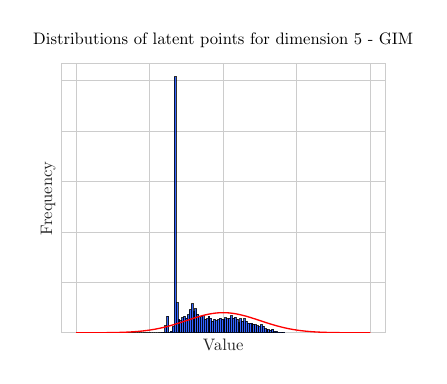
\begin{tikzpicture}[scale=0.6]

\definecolor{blue262255}{RGB}{2,62,255}
\definecolor{darkslategray38}{RGB}{38,38,38}
\definecolor{lightgray204}{RGB}{204,204,204}

\begin{axis}[
axis line style={lightgray204},
tick align=outside,
title={Distributions of latent points for dimension 5 - GIM},
x grid style={lightgray204},
xlabel=\textcolor{darkslategray38}{Value},
xmajorgrids,
xmajorticks=false,
xmin=-4.4, xmax=4.4,
xtick style={color=darkslategray38},
y grid style={lightgray204},
ylabel=\textcolor{darkslategray38}{Frequency},
ymajorgrids,
ymajorticks=false,
ymin=0, ymax=5.33037062452773,
ytick style={color=darkslategray38}
]
\draw[draw=black,fill=blue262255,opacity=0.8,line width=0.48pt] (axis cs:-3.41899585723877,0) rectangle (axis cs:-3.36807417869568,0.00261004804726538);
\draw[draw=black,fill=blue262255,opacity=0.8,line width=0.48pt] (axis cs:-3.36807441711426,0) rectangle (axis cs:-3.31715273857117,0);
\draw[draw=black,fill=blue262255,opacity=0.8,line width=0.48pt] (axis cs:-3.31715250015259,0) rectangle (axis cs:-3.2662308216095,0);
\draw[draw=black,fill=blue262255,opacity=0.8,line width=0.48pt] (axis cs:-3.26623106002808,0) rectangle (axis cs:-3.21530914306641,0);
\draw[draw=black,fill=blue262255,opacity=0.8,line width=0.48pt] (axis cs:-3.21530914306641,0) rectangle (axis cs:-3.16438746452332,0);
\draw[draw=black,fill=blue262255,opacity=0.8,line width=0.48pt] (axis cs:-3.16438722610474,0) rectangle (axis cs:-3.11346554756165,0);
\draw[draw=black,fill=blue262255,opacity=0.8,line width=0.48pt] (axis cs:-3.11346578598022,0) rectangle (axis cs:-3.06254410743713,0.00261004804726538);
\draw[draw=black,fill=blue262255,opacity=0.8,line width=0.48pt] (axis cs:-3.06254386901855,0) rectangle (axis cs:-3.01162219047546,0);
\draw[draw=black,fill=blue262255,opacity=0.8,line width=0.48pt] (axis cs:-3.01162242889404,0) rectangle (axis cs:-2.96070075035095,0);
\draw[draw=black,fill=blue262255,opacity=0.8,line width=0.48pt] (axis cs:-2.96070051193237,0) rectangle (axis cs:-2.90977883338928,0);
\draw[draw=black,fill=blue262255,opacity=0.8,line width=0.48pt] (axis cs:-2.90977907180786,0) rectangle (axis cs:-2.85885739326477,0);
\draw[draw=black,fill=blue262255,opacity=0.8,line width=0.48pt] (axis cs:-2.85885739326477,0) rectangle (axis cs:-2.8079354763031,0);
\draw[draw=black,fill=blue262255,opacity=0.8,line width=0.48pt] (axis cs:-2.80793523788452,0) rectangle (axis cs:-2.75701355934143,0);
\draw[draw=black,fill=blue262255,opacity=0.8,line width=0.48pt] (axis cs:-2.75701379776001,0) rectangle (axis cs:-2.70609211921692,0);
\draw[draw=black,fill=blue262255,opacity=0.8,line width=0.48pt] (axis cs:-2.70609188079834,0) rectangle (axis cs:-2.65517020225525,0);
\draw[draw=black,fill=blue262255,opacity=0.8,line width=0.48pt] (axis cs:-2.65517044067383,0) rectangle (axis cs:-2.60424876213074,0);
\draw[draw=black,fill=blue262255,opacity=0.8,line width=0.48pt] (axis cs:-2.60424852371216,0) rectangle (axis cs:-2.55332684516907,0);
\draw[draw=black,fill=blue262255,opacity=0.8,line width=0.48pt] (axis cs:-2.55332708358765,0) rectangle (axis cs:-2.50240540504456,0);
\draw[draw=black,fill=blue262255,opacity=0.8,line width=0.48pt] (axis cs:-2.50240516662598,0) rectangle (axis cs:-2.45148348808289,0);
\draw[draw=black,fill=blue262255,opacity=0.8,line width=0.48pt] (axis cs:-2.45148372650146,0) rectangle (axis cs:-2.40056180953979,0);
\draw[draw=black,fill=blue262255,opacity=0.8,line width=0.48pt] (axis cs:-2.40056180953979,0) rectangle (axis cs:-2.3496401309967,0);
\draw[draw=black,fill=blue262255,opacity=0.8,line width=0.48pt] (axis cs:-2.34963989257812,0) rectangle (axis cs:-2.29871821403503,0);
\draw[draw=black,fill=blue262255,opacity=0.8,line width=0.48pt] (axis cs:-2.29871845245361,0) rectangle (axis cs:-2.24779677391052,0);
\draw[draw=black,fill=blue262255,opacity=0.8,line width=0.48pt] (axis cs:-2.24779653549194,0) rectangle (axis cs:-2.19687485694885,0);
\draw[draw=black,fill=blue262255,opacity=0.8,line width=0.48pt] (axis cs:-2.19687509536743,0) rectangle (axis cs:-2.14595341682434,0);
\draw[draw=black,fill=blue262255,opacity=0.8,line width=0.48pt] (axis cs:-2.14595317840576,0) rectangle (axis cs:-2.09503149986267,0);
\draw[draw=black,fill=blue262255,opacity=0.8,line width=0.48pt] (axis cs:-2.09503173828125,0) rectangle (axis cs:-2.04410982131958,0);
\draw[draw=black,fill=blue262255,opacity=0.8,line width=0.48pt] (axis cs:-2.04410982131958,0) rectangle (axis cs:-1.99318838119507,0.00261005415748623);
\draw[draw=black,fill=blue262255,opacity=0.8,line width=0.48pt] (axis cs:-1.99318838119507,0) rectangle (axis cs:-1.9422664642334,0);
\draw[draw=black,fill=blue262255,opacity=0.8,line width=0.48pt] (axis cs:-1.9422664642334,0) rectangle (axis cs:-1.89134478569031,0);
\draw[draw=black,fill=blue262255,opacity=0.8,line width=0.48pt] (axis cs:-1.89134478569031,0) rectangle (axis cs:-1.84042310714722,0);
\draw[draw=black,fill=blue262255,opacity=0.8,line width=0.48pt] (axis cs:-1.84042310714722,0) rectangle (axis cs:-1.78950142860413,0);
\draw[draw=black,fill=blue262255,opacity=0.8,line width=0.48pt] (axis cs:-1.78950142860413,0) rectangle (axis cs:-1.73857951164246,0);
\draw[draw=black,fill=blue262255,opacity=0.8,line width=0.48pt] (axis cs:-1.73857963085175,0) rectangle (axis cs:-1.68765795230865,0);
\draw[draw=black,fill=blue262255,opacity=0.8,line width=0.48pt] (axis cs:-1.68765795230865,0) rectangle (axis cs:-1.63673627376556,0.00783014414179615);
\draw[draw=black,fill=blue262255,opacity=0.8,line width=0.48pt] (axis cs:-1.63673627376556,0) rectangle (axis cs:-1.58581459522247,0.00522009609453077);
\draw[draw=black,fill=blue262255,opacity=0.8,line width=0.48pt] (axis cs:-1.58581471443176,0) rectangle (axis cs:-1.53489279747009,0.143552306539023);
\draw[draw=black,fill=blue262255,opacity=0.8,line width=0.48pt] (axis cs:-1.53489279747009,0) rectangle (axis cs:-1.483971118927,0.323645957860907);
\draw[draw=black,fill=blue262255,opacity=0.8,line width=0.48pt] (axis cs:-1.483971118927,0) rectangle (axis cs:-1.43304944038391,0.0104401921890615);
\draw[draw=black,fill=blue262255,opacity=0.8,line width=0.48pt] (axis cs:-1.43304944038391,0) rectangle (axis cs:-1.38212776184082,0.0365406726617154);
\draw[draw=black,fill=blue262255,opacity=0.8,line width=0.48pt] (axis cs:-1.38212776184082,0) rectangle (axis cs:-1.33120584487915,0.120061929105365);
\draw[draw=black,fill=blue262255,opacity=0.8,line width=0.48pt] (axis cs:-1.33120596408844,0) rectangle (axis cs:-1.28028428554535,5.07654345193117);
\draw[draw=black,fill=blue262255,opacity=0.8,line width=0.48pt] (axis cs:-1.28028428554535,0) rectangle (axis cs:-1.22936260700226,0.595090954776507);
\draw[draw=black,fill=blue262255,opacity=0.8,line width=0.48pt] (axis cs:-1.22936260700226,0) rectangle (axis cs:-1.17844092845917,0.274055044962865);
\draw[draw=black,fill=blue262255,opacity=0.8,line width=0.48pt] (axis cs:-1.17844104766846,0) rectangle (axis cs:-1.12751913070679,0.237513816273656);
\draw[draw=black,fill=blue262255,opacity=0.8,line width=0.48pt] (axis cs:-1.12751913070679,0) rectangle (axis cs:-1.0765974521637,0.300155525435519);
\draw[draw=black,fill=blue262255,opacity=0.8,line width=0.48pt] (axis cs:-1.0765974521637,0) rectangle (axis cs:-1.02567577362061,0.326256005908173);
\draw[draw=black,fill=blue262255,opacity=0.8,line width=0.48pt] (axis cs:-1.02567577362061,0) rectangle (axis cs:-0.974754095077515,0.292325039122557);
\draw[draw=black,fill=blue262255,opacity=0.8,line width=0.48pt] (axis cs:-0.97475403547287,0) rectangle (axis cs:-0.923832356929779,0.360186630522623);
\draw[draw=black,fill=blue262255,opacity=0.8,line width=0.48pt] (axis cs:-0.923832297325134,0) rectangle (axis cs:-0.872910618782043,0.456757873628995);
\draw[draw=black,fill=blue262255,opacity=0.8,line width=0.48pt] (axis cs:-0.872910618782043,0) rectangle (axis cs:-0.821988940238953,0.579429988260783);
\draw[draw=black,fill=blue262255,opacity=0.8,line width=0.48pt] (axis cs:-0.821988880634308,0) rectangle (axis cs:-0.771067202091217,0.430657927798788);
\draw[draw=black,fill=blue262255,opacity=0.8,line width=0.48pt] (axis cs:-0.771067142486572,0) rectangle (axis cs:-0.720145463943481,0.480248278558487);
\draw[draw=black,fill=blue262255,opacity=0.8,line width=0.48pt] (axis cs:-0.720145463943481,0) rectangle (axis cs:-0.669223785400391,0.370626822711684);
\draw[draw=black,fill=blue262255,opacity=0.8,line width=0.48pt] (axis cs:-0.669223785400391,0) rectangle (axis cs:-0.6183021068573,0.32103553403638);
\draw[draw=black,fill=blue262255,opacity=0.8,line width=0.48pt] (axis cs:-0.618302047252655,0) rectangle (axis cs:-0.567380368709564,0.323645957860907);
\draw[draw=black,fill=blue262255,opacity=0.8,line width=0.48pt] (axis cs:-0.567380309104919,0) rectangle (axis cs:-0.516458630561829,0.341915893973705);
\draw[draw=black,fill=blue262255,opacity=0.8,line width=0.48pt] (axis cs:-0.516458630561829,0) rectangle (axis cs:-0.465536952018738,0.2714449969156);
\draw[draw=black,fill=blue262255,opacity=0.8,line width=0.48pt] (axis cs:-0.465536952018738,0) rectangle (axis cs:-0.414615273475647,0.276664931089752);
\draw[draw=black,fill=blue262255,opacity=0.8,line width=0.48pt] (axis cs:-0.414615213871002,0) rectangle (axis cs:-0.363693535327911,0.334085954523474);
\draw[draw=black,fill=blue262255,opacity=0.8,line width=0.48pt] (axis cs:-0.363693535327911,0) rectangle (axis cs:-0.312771856784821,0.29232521020804);
\draw[draw=black,fill=blue262255,opacity=0.8,line width=0.48pt] (axis cs:-0.312771797180176,0) rectangle (axis cs:-0.261850118637085,0.234904186774318);
\draw[draw=black,fill=blue262255,opacity=0.8,line width=0.48pt] (axis cs:-0.261850088834763,0) rectangle (axis cs:-0.210928410291672,0.263614621349934);
\draw[draw=black,fill=blue262255,opacity=0.8,line width=0.48pt] (axis cs:-0.210928380489349,0) rectangle (axis cs:-0.160006701946259,0.242734326333462);
\draw[draw=black,fill=blue262255,opacity=0.8,line width=0.48pt] (axis cs:-0.160006672143936,0) rectangle (axis cs:-0.109084993600845,0.255784558932035);
\draw[draw=black,fill=blue262255,opacity=0.8,line width=0.48pt] (axis cs:-0.109084963798523,0) rectangle (axis cs:-0.0581632852554321,0.294935235151114);
\draw[draw=black,fill=blue262255,opacity=0.8,line width=0.48pt] (axis cs:-0.0581632517278194,0) rectangle (axis cs:-0.00724157318472862,0.268834791530608);
\draw[draw=black,fill=blue262255,opacity=0.8,line width=0.48pt] (axis cs:-0.00724154151976109,0) rectangle (axis cs:0.0436801388859749,0.274054884570037);
\draw[draw=black,fill=blue262255,opacity=0.8,line width=0.48pt] (axis cs:0.0436801686882973,0) rectangle (axis cs:0.0946018472313881,0.297545303247469);
\draw[draw=black,fill=blue262255,opacity=0.8,line width=0.48pt] (axis cs:0.0946018844842911,0) rectangle (axis cs:0.145523563027382,0.279274936747514);
\draw[draw=black,fill=blue262255,opacity=0.8,line width=0.48pt] (axis cs:0.145523592829704,0) rectangle (axis cs:0.196445271372795,0.287105117168611);
\draw[draw=black,fill=blue262255,opacity=0.8,line width=0.48pt] (axis cs:0.196445301175117,0) rectangle (axis cs:0.247366979718208,0.341916094082618);
\draw[draw=black,fill=blue262255,opacity=0.8,line width=0.48pt] (axis cs:0.247367024421692,0) rectangle (axis cs:0.298288702964783,0.287105117168611);
\draw[draw=black,fill=blue262255,opacity=0.8,line width=0.48pt] (axis cs:0.298288702964783,0) rectangle (axis cs:0.349210381507874,0.313205582365757);
\draw[draw=black,fill=blue262255,opacity=0.8,line width=0.48pt] (axis cs:0.349210441112518,0) rectangle (axis cs:0.400132119655609,0.274054884570037);
\draw[draw=black,fill=blue262255,opacity=0.8,line width=0.48pt] (axis cs:0.400132119655609,0) rectangle (axis cs:0.4510537981987,0.200973582018027);
\draw[draw=black,fill=blue262255,opacity=0.8,line width=0.48pt] (axis cs:0.451053857803345,0) rectangle (axis cs:0.501975536346436,0.276664931089752);
\draw[draw=black,fill=blue262255,opacity=0.8,line width=0.48pt] (axis cs:0.501975536346436,0) rectangle (axis cs:0.552897214889526,0.224463869326249);
\draw[draw=black,fill=blue262255,opacity=0.8,line width=0.48pt] (axis cs:0.552897274494171,0) rectangle (axis cs:0.603818953037262,0.276665093010131);
\draw[draw=black,fill=blue262255,opacity=0.8,line width=0.48pt] (axis cs:0.603819012641907,0) rectangle (axis cs:0.654740691184998,0.229683959310581);
\draw[draw=black,fill=blue262255,opacity=0.8,line width=0.48pt] (axis cs:0.654740691184998,0) rectangle (axis cs:0.705662369728088,0.195753603544904);
\draw[draw=black,fill=blue262255,opacity=0.8,line width=0.48pt] (axis cs:0.705662369728088,0) rectangle (axis cs:0.756584048271179,0.18792323943593);
\draw[draw=black,fill=blue262255,opacity=0.8,line width=0.48pt] (axis cs:0.756584107875824,0) rectangle (axis cs:0.807505786418915,0.187923459403108);
\draw[draw=black,fill=blue262255,opacity=0.8,line width=0.48pt] (axis cs:0.80750584602356,0) rectangle (axis cs:0.85842752456665,0.167042879498604);
\draw[draw=black,fill=blue262255,opacity=0.8,line width=0.48pt] (axis cs:0.85842752456665,0) rectangle (axis cs:0.909349203109741,0.159212930883188);
\draw[draw=black,fill=blue262255,opacity=0.8,line width=0.48pt] (axis cs:0.909349203109741,0) rectangle (axis cs:0.960270881652832,0.143552474569113);
\draw[draw=black,fill=blue262255,opacity=0.8,line width=0.48pt] (axis cs:0.960271000862122,0) rectangle (axis cs:1.01119267940521,0.120062069639622);
\draw[draw=black,fill=blue262255,opacity=0.8,line width=0.48pt] (axis cs:1.01119267940521,0) rectangle (axis cs:1.0621143579483,0.156602882835923);
\draw[draw=black,fill=blue262255,opacity=0.8,line width=0.48pt] (axis cs:1.0621143579483,0) rectangle (axis cs:1.11303603649139,0.1357224984578);
\draw[draw=black,fill=blue262255,opacity=0.8,line width=0.48pt] (axis cs:1.11303603649139,0) rectangle (axis cs:1.16395771503448,0.0783014414179615);
\draw[draw=black,fill=blue262255,opacity=0.8,line width=0.48pt] (axis cs:1.1639575958252,0) rectangle (axis cs:1.21487951278687,0.0678610903639018);
\draw[draw=black,fill=blue262255,opacity=0.8,line width=0.48pt] (axis cs:1.21487951278687,0) rectangle (axis cs:1.26580119132996,0.0652512011816346);
\draw[draw=black,fill=blue262255,opacity=0.8,line width=0.48pt] (axis cs:1.26580119132996,0) rectangle (axis cs:1.31672286987305,0.0522009609453077);
\draw[draw=black,fill=blue262255,opacity=0.8,line width=0.48pt] (axis cs:1.31672286987305,0) rectangle (axis cs:1.36764454841614,0.0756913933706961);
\draw[draw=black,fill=blue262255,opacity=0.8,line width=0.48pt] (axis cs:1.36764454841614,0) rectangle (axis cs:1.41856646537781,0.036540587119024);
\draw[draw=black,fill=blue262255,opacity=0.8,line width=0.48pt] (axis cs:1.41856634616852,0) rectangle (axis cs:1.46948802471161,0.03393062461445);
\draw[draw=black,fill=blue262255,opacity=0.8,line width=0.48pt] (axis cs:1.46948802471161,0) rectangle (axis cs:1.5204097032547,0.0156602882835923);
\draw[draw=black,fill=blue262255,opacity=0.8,line width=0.48pt] (axis cs:1.5204097032547,0) rectangle (axis cs:1.57133138179779,0.0130502402363269);
\draw[draw=black,fill=blue262255,opacity=0.8,line width=0.48pt] (axis cs:1.5713312625885,0) rectangle (axis cs:1.62225317955017,0.0156602516224389);
\draw[draw=black,fill=blue262255,opacity=0.8,line width=0.48pt] (axis cs:1.62225317955017,0) rectangle (axis cs:1.67317485809326,0.0104401921890615);
\addplot [thick, red]
table {%
-4 0.000133830225764885
-3.99199199199199 0.000138182046410498
-3.98398398398398 0.000142666228042307
-3.97597597597598 0.000147286481503254
-3.96796796796797 0.000152046611333821
-3.95995995995996 0.000156950517814782
-3.95195195195195 0.00016200219904485
-3.94394394394394 0.00016720575305353
-3.93593593593594 0.000172565379949496
-3.92792792792793 0.00017808538410479
-3.91991991991992 0.000183770176375138
-3.91191191191191 0.000189624276356684
-3.9039039039039 0.000195652314679408
-3.8958958958959 0.000201859035337517
-3.88788788788789 0.000208249298057069
-3.87987987987988 0.000214828080701088
-3.87187187187187 0.000221600481712426
-3.86386386386386 0.0002285717225946
-3.85585585585586 0.000235747150430845
-3.84784784784785 0.000243132240441603
-3.83983983983984 0.000250732598580649
-3.83183183183183 0.000258553964170059
-3.82382382382382 0.000266602212574213
-3.81581581581582 0.000274883357912987
-3.80780780780781 0.000283403555814325
-3.7997997997998 0.000292169106206322
-3.79179179179179 0.000301186456148957
-3.78378378378378 0.0003104622027056
-3.77577577577578 0.000320003095854415
-3.76776776776777 0.000329816041439723
-3.75975975975976 0.000339908104163431
-3.75175175175175 0.00035028651061658
-3.74374374374374 0.000360958652351047
-3.73573573573574 0.000371932088991451
-3.72772772772773 0.000383214551387261
-3.71971971971972 0.000394813944805093
-3.71171171171171 0.000406738352161197
-3.7037037037037 0.000418996037294058
-3.6956956956957 0.00043159544827708
-3.68768768768769 0.00044454522077123
-3.67967967967968 0.000457854181417586
-3.67167167167167 0.000471531351269624
-3.66366366366366 0.000485585949265103
-3.65565565565566 0.000500027395737409
-3.64764764764765 0.000514865315966112
-3.63963963963964 0.000530109543766577
-3.63163163163163 0.000545770125118336
-3.62362362362362 0.000561857321831991
-3.61561561561562 0.00057838161525435
-3.60760760760761 0.000595353710011453
-3.5995995995996 0.000612784537789192
-3.59159159159159 0.000630685261151105
-3.58358358358358 0.000649067277392973
-3.57557557557558 0.000667942222433796
-3.56756756756757 0.000687321974742665
-3.55955955955956 0.000707218659301081
-3.55155155155155 0.000727644651600166
-3.54354354354354 0.000748612581672245
-3.53553553553554 0.000770135338156225
-3.52752752752753 0.000792226072396121
-3.51951951951952 0.00081489820257214
-3.51151151151151 0.000838165417863603
-3.5035035035035 0.000862041682643007
-3.4954954954955 0.000886541240700502
-3.48748748748749 0.00091167861949796
-3.47947947947948 0.000937468634451866
-3.47147147147147 0.000963926393244149
-3.46346346346346 0.000991067300160059
-3.45545545545546 0.0010189070604522
-3.44744744744745 0.00104746168472971
-3.43943943943944 0.0010767474933716
-3.43143143143143 0.00110678112096323
-3.42342342342342 0.00113757952075483
-3.41541541541542 0.00116915996914087
-3.40740740740741 0.00120154007015926
-3.3993993993994 0.00123473776000907
-3.39139139139139 0.00126877131158549
-3.38338338338338 0.00130365933903088
-3.37537537537538 0.00133942080230046
-3.36736736736737 0.00137607501174126
-3.35935935935936 0.001413641632683
-3.35135135135135 0.00145214069003938
-3.34334334334334 0.0014915925729182
-3.33533533533534 0.00153201803923895
-3.32732732732733 0.00157343822035606
-3.31931931931932 0.00161587462568624
-3.31131131131131 0.00165934914733831
-3.3033033033033 0.00170388406474362
-3.2952952952953 0.00174950204928538
-3.28728728728729 0.00179622616892505
-3.27927927927928 0.00184407989282385
-3.27127127127127 0.00189308709595757
-3.26326326326326 0.00194327206372255
-3.25525525525526 0.00199465949653091
-3.24724724724725 0.00204727451439301
-3.23923923923924 0.00210114266148476
-3.23123123123123 0.00215628991069791
-3.22322322322322 0.00221274266817093
-3.21521521521522 0.00227052777779815
-3.20720720720721 0.00232967252571501
-3.1991991991992 0.00239020464475689
-3.19119119119119 0.00245215231888918
-3.18318318318318 0.00251554418760605
-3.17517517517518 0.00258040935029545
-3.16716716716717 0.00264677737056774
-3.15915915915916 0.00271467828054534
-3.15115115115115 0.00278414258511061
-3.14314314314314 0.00285520126610952
-3.13513513513514 0.00292788578650791
-3.12712712712713 0.00300222809449793
-3.11911911911912 0.00307826062755151
-3.11111111111111 0.00315601631641804
-3.1031031031031 0.00323552858906328
-3.0950950950951 0.00331683137454643
-3.08708708708709 0.00339995910683238
-3.07907907907908 0.00348494672853595
-3.07107107107107 0.00357182969459489
-3.06306306306306 0.00366064397586864
-3.05505505505506 0.00375142606265932
-3.04704704704705 0.00384421296815189
-3.03903903903904 0.00393904223176991
-3.03103103103103 0.00403595192244368
-3.02302302302302 0.0041349806417872
-3.01501501501502 0.00423616752718052
-3.00700700700701 0.00433955225475399
-2.998998998999 0.00444517504227068
-2.99099099099099 0.00455307665190355
-2.98298298298298 0.00466329839290368
-2.97497497497497 0.00477588212415564
-2.96696696696697 0.00489087025661667
-2.95895895895896 0.00500830575563558
-2.95095095095095 0.00512823214314763
-2.94294294294294 0.00525069349974172
-2.93493493493493 0.00537573446659573
-2.92692692692693 0.00550340024727644
-2.91891891891892 0.00563373660939975
-2.91091091091091 0.0057667898861475
-2.9029029029029 0.00590260697763674
-2.89489489489489 0.00604123535213746
-2.88688688688689 0.00618272304713484
-2.87887887887888 0.00632711867023164
-2.87087087087087 0.00647447139988703
-2.86286286286286 0.00662483098598741
-2.85485485485485 0.0067782477502453
-2.84684684684685 0.0069347725864219
-2.83883883883884 0.00709445696036946
-2.83083083083083 0.00725735290988893
-2.82282282282282 0.00742351304439893
-2.81481481481481 0.00759299054441176
-2.80680680680681 0.0077658391608121
-2.7987987987988 0.00794211321393437
-2.79079079079079 0.00812186759243432
-2.78278278278278 0.00830515775195071
-2.77477477477477 0.00849203971355293
-2.76676676676677 0.00868257006197001
-2.75875875875876 0.00887680594359712
-2.75075075075075 0.00907480506427511
-2.74274274274274 0.00927662568683898
-2.73473473473473 0.00948232662843099
-2.72672672672673 0.00969196725757422
-2.71871871871872 0.00990560749100246
-2.71071071071071 0.0101233077902421
-2.7027027027027 0.0103451291579421
-2.69469469469469 0.0105711331339476
-2.68668668668669 0.0108013817911136
-2.67867867867868 0.011035937730854
-2.67067067067067 0.0112748640784219
-2.66266266266266 0.0115182244779185
-2.65465465465465 0.0117660830870247
-2.64664664664665 0.0120185045714526
-2.63863863863864 0.0122755540991133
-2.63063063063063 0.0125372973339956
-2.62262262262262 0.0128038004297541
-2.61461461461461 0.0130751300230007
-2.60660660660661 0.0133513532262973
-2.5985985985986 0.0136325376208454
-2.59059059059059 0.0139187512488692
-2.58258258258258 0.014210062605689
-2.57457457457457 0.0145065406314803
-2.56656656656657 0.0148082547027168
-2.55855855855856 0.0151152746232934
-2.55055055055055 0.0154276706153247
-2.54254254254254 0.0157455133096184
-2.53453453453453 0.0160688737358178
-2.52652652652653 0.016397823312213
-2.51851851851852 0.0167324338352151
-2.51051051051051 0.0170727774684938
-2.5025025025025 0.0174189267317727
-2.49449449449449 0.0177709544892815
-2.48648648648649 0.0181289339378627
-2.47847847847848 0.0184929385947284
-2.47047047047047 0.0188630422848682
-2.46246246246246 0.0192393191281025
-2.45445445445445 0.0196218435257817
-2.44644644644645 0.0200106901471285
-2.43843843843844 0.020405933915221
-2.43043043043043 0.0208076499926159
-2.42242242242242 0.0212159137666093
-2.41441441441441 0.0216308008341344
-2.40640640640641 0.0220523869862944
-2.3983983983984 0.0224807481925294
-2.39039039039039 0.022915960584417
-2.38238238238238 0.0233581004391047
-2.37437437437437 0.023807244162374
-2.36636636636637 0.0242634682713357
-2.35835835835836 0.0247268493767558
-2.35035035035035 0.0251974641650118
-2.34234234234234 0.0256753893796796
-2.33433433433433 0.0261607018027501
-2.32632632632633 0.0266534782354775
-2.31831831831832 0.0271537954788581
-2.31031031031031 0.0276617303137407
-2.3023023023023 0.0281773594805703
-2.29429429429429 0.0287007596587648
-2.28628628628629 0.0292320074457259
-2.27827827827828 0.029771179335487
-2.27027027027027 0.0303183516969979
-2.26226226226226 0.0308736007520491
-2.25425425425425 0.0314370025528369
-2.24624624624625 0.0320086329591723
-2.23823823823824 0.0325885676153351
-2.23023023023023 0.0331768819265761
-2.22222222222222 0.0337736510352706
-2.21421421421421 0.0343789497967251
-2.20620620620621 0.0349928527546413
-2.1981981981982 0.0356154341162401
-2.19019019019019 0.0362467677270497
-2.18218218218218 0.0368869270453615
-2.17417417417417 0.0375359851163567
-2.16616616616617 0.03819401454591
-2.15815815815816 0.0388610874740724
-2.15015015015015 0.03953727554824
-2.14214214214214 0.0402226498960119
-2.13413413413413 0.0409172810977437
-2.12612612612613 0.0416212391588003
-2.11811811811812 0.0423345934815158
-2.11011011011011 0.0430574128368641
-2.1021021021021 0.043789765335848
-2.09409409409409 0.0445317184006117
-2.08608608608609 0.0452833387352837
-2.07807807807808 0.0460446922965577
-2.07007007007007 0.0468158442640166
-2.06206206206206 0.0475968590102091
-2.05405405405405 0.0483878000704834
-2.04604604604605 0.0491887301125894
-2.03803803803804 0.0499997109060533
-2.03003003003003 0.0508208032913361
-2.02202202202202 0.0516520671487823
-2.01401401401401 0.0524935613673682
-2.00600600600601 0.053345343813258
-1.997997997998 0.0542074712981785
-1.98998998998999 0.0550799995476186
-1.98198198198198 0.0559629831688668
-1.97397397397397 0.0568564756188931
-1.96596596596597 0.0577605291720876
-1.95795795795796 0.0586751948878651
-1.94994994994995 0.0596005225781457
-1.94194194194194 0.0605365607747232
-1.93393393393393 0.0614833566965309
-1.92592592592593 0.062440956216817
-1.91791791791792 0.06340940383024
-1.90990990990991 0.0643887426198963
-1.9019019019019 0.0653790142242912
-1.89389389389389 0.0663802588042656
-1.88588588588589 0.0673925150098903
-1.87787787787788 0.0684158199473405
-1.86986986986987 0.0694502091457625
-1.86186186186186 0.0704957165241465
-1.85385385385385 0.0715523743582165
-1.84584584584585 0.0726202132473521
-1.83783783783784 0.0736992620815557
-1.82982982982983 0.0747895480084762
-1.82182182182182 0.0758910964005057
-1.81381381381381 0.0770039308219614
-1.80580580580581 0.0781280729963669
-1.7977977977978 0.0792635427738473
-1.78978978978979 0.0804103580986525
-1.78178178178178 0.0815685349768227
-1.77377377377377 0.0827380874440109
-1.76576576576577 0.0839190275334777
-1.75775775775776 0.0851113652442723
-1.74974974974975 0.086315108509615
-1.74174174174174 0.0875302631654975
-1.73373373373373 0.0887568329195139
-1.72572572572573 0.0899948193199405
-1.71771771771772 0.0912442217250772
-1.70970970970971 0.0925050372728685
-1.7017017017017 0.0937772608508177
-1.69369369369369 0.0950608850662112
-1.68568568568569 0.0963559002166691
-1.67767767767768 0.0976622942610365
-1.66966966966967 0.0989800527906321
-1.66166166166166 0.100309159000872
-1.65365365365365 0.10164959366328
-1.64564564564565 0.103001335097907
-1.63763763763764 0.10436435914617
-1.62962962962963 0.105738639144131
-1.62162162162162 0.107124145896225
-1.61361361361361 0.108520847649465
-1.60560560560561 0.10992871006813
-1.5975975975976 0.111347696208955
-1.58958958958959 0.112777766496842
-1.58158158158158 0.114218878701105
-1.57357357357357 0.115670987912262
-1.56556556556557 0.117134046519405
-1.55755755755756 0.11860800418814
-1.54954954954955 0.120092807839133
-1.54154154154154 0.121588401627275
-1.53353353353353 0.123094726921466
-1.52552552552553 0.124611722285057
-1.51751751751752 0.12613932345695
-1.50950950950951 0.127677463333369
-1.5015015015015 0.129226071950339
-1.49349349349349 0.130785076466857
-1.48548548548549 0.132354401148798
-1.47747747747748 0.133933967353555
-1.46946946946947 0.13552369351543
-1.46146146146146 0.137123495131801
-1.45345345345345 0.13873328475006
-1.44544544544545 0.140352971955359
-1.43743743743744 0.141982463359159
-1.42942942942943 0.143621662588612
-1.42142142142142 0.14527047027677
-1.41341341341341 0.146928784053658
-1.40540540540541 0.148596498538208
-1.3973973973974 0.150273505331067
-1.38938938938939 0.151959693008306
-1.38138138138138 0.153654947116025
-1.37337337337337 0.155359150165875
-1.36536536536537 0.157072181631514
-1.35735735735736 0.158793917945997
-1.34934934934935 0.160524232500121
-1.34134134134134 0.16226299564173
-1.33333333333333 0.164010074675994
-1.32532532532533 0.165765333866673
-1.31731731731732 0.167528634438376
-1.30930930930931 0.169299834579821
-1.3013013013013 0.17107878944811
-1.29329329329329 0.172865351174024
-1.28528528528529 0.174659368868355
-1.27727727727728 0.176460688629273
-1.26926926926927 0.178269153550739
-1.26126126126126 0.180084603731981
-1.25325325325325 0.181906876288021
-1.24524524524525 0.183735805361283
-1.23723723723724 0.185571222134271
-1.22922922922923 0.187412954843324
-1.22122122122122 0.18926082879347
-1.21321321321321 0.191114666374361
-1.20520520520521 0.192974287077311
-1.1971971971972 0.194839507513435
-1.18918918918919 0.19671014143289
-1.18118118118118 0.198585999745227
-1.17317317317317 0.200466890540856
-1.16516516516517 0.202352619113618
-1.15715715715716 0.204242987984477
-1.14914914914915 0.206137796926331
-1.14114114114114 0.208036842989938
-1.13313313313313 0.209939920530956
-1.12512512512513 0.21184682123811
-1.11711711711712 0.21375733416247
-1.10910910910911 0.215671245747847
-1.1011011011011 0.217588339862305
-1.09309309309309 0.219508397830784
-1.08508508508509 0.221431198468836
-1.07707707707708 0.223356518117463
-1.06906906906907 0.225284130679063
-1.06106106106106 0.22721380765447
-1.05305305305305 0.229145318181096
-1.04504504504505 0.231078429072154
-1.03703703703704 0.233012904856966
-1.02902902902903 0.234948507822352
-1.02102102102102 0.236884998055083
-1.01301301301301 0.238822133485401
-1.00500500500501 0.24075966993159
-0.996996996996997 0.242697361145593
-0.988988988988989 0.244634958859672
-0.980980980980981 0.246572212834085
-0.972972972972973 0.248508870905785
-0.964964964964965 0.250444679038131
-0.956956956956957 0.252379381371581
-0.948948948948949 0.254312720275385
-0.940940940940941 0.256244436400228
-0.932932932932933 0.258174268731856
-0.924924924924925 0.260101954645624
-0.916916916916917 0.262027229961987
-0.908908908908909 0.263949829002911
-0.900900900900901 0.265869484649172
-0.892892892892893 0.267785928398552
-0.884884884884885 0.269698890424904
-0.876876876876877 0.271608099638066
-0.868868868868869 0.273513283744617
-0.860860860860861 0.275414169309444
-0.852852852852853 0.277310481818125
-0.844844844844845 0.279201945740075
-0.836836836836837 0.281088284592474
-0.828828828828829 0.28296922100493
-0.820820820820821 0.284844476784867
-0.812812812812813 0.286713772983616
-0.804804804804805 0.288576829963198
-0.796796796796797 0.290433367463758
-0.788788788788789 0.292283104671645
-0.780780780780781 0.294125760288111
-0.772772772772773 0.295961052598604
-0.764764764764765 0.29778869954263
-0.756756756756757 0.299608418784177
-0.748748748748749 0.301419927782648
-0.740740740740741 0.303222943864308
-0.732732732732733 0.305017184294205
-0.724724724724725 0.306802366348536
-0.716716716716717 0.308578207387456
-0.708708708708709 0.310344424928268
-0.700700700700701 0.312100736719007
-0.692692692692693 0.313846860812361
-0.684684684684685 0.31558251563992
-0.676676676676677 0.317307420086723
-0.668668668668669 0.319021293566066
-0.660660660660661 0.320723856094559
-0.652652652652653 0.322414828367396
-0.644644644644645 0.324093931833804
-0.636636636636636 0.325760888772662
-0.628628628628629 0.327415422368237
-0.620620620620621 0.329057256786028
-0.612612612612613 0.330686117248681
-0.604604604604605 0.33230173011195
-0.596596596596596 0.333903822940662
-0.588588588588589 0.335492124584683
-0.580580580580581 0.337066365254824
-0.572572572572573 0.338626276598684
-0.564564564564565 0.340171591776383
-0.556556556556556 0.341702045536168
-0.548548548548549 0.343217374289848
-0.54054054054054 0.344717316188045
-0.532532532532533 0.346201611195215
-0.524524524524525 0.347670001164422
-0.516516516516516 0.349122229911825
-0.508508508508509 0.350558043290856
-0.5005005005005 0.351977189266054
-0.492492492492492 0.353379417986526
-0.484484484484485 0.354764481859011
-0.476476476476476 0.356132135620502
-0.468468468468469 0.357482136410418
-0.46046046046046 0.358814243842273
-0.452452452452452 0.360128220074839
-0.444444444444445 0.361423829882744
-0.436436436436436 0.362700840726495
-0.428428428428429 0.363959022821904
-0.42042042042042 0.365198149208855
-0.412412412412412 0.366417995819425
-0.404404404404405 0.3676183415453
-0.396396396396396 0.368798968304465
-0.388388388388389 0.369959661107154
-0.38038038038038 0.37110020812101
-0.372372372372372 0.372220400735444
-0.364364364364365 0.373320033625156
-0.356356356356356 0.374398904812801
-0.348348348348348 0.375456815730761
-0.34034034034034 0.376493571282005
-0.332332332332332 0.377508979900006
-0.324324324324325 0.378502853607702
-0.316316316316316 0.379475008075448
-0.308308308308308 0.380425262677969
-0.3003003003003 0.38135344055026
-0.292292292292292 0.382259368642425
-0.284284284284285 0.38314287777343
-0.276276276276276 0.384003802683735
-0.268268268268268 0.3848419820868
-0.26026026026026 0.385657258719425
-0.252252252252252 0.386449479390916
-0.244244244244244 0.387218495031049
-0.236236236236236 0.387964160736805
-0.228228228228228 0.38868633581787
-0.22022022022022 0.389384883840873
-0.212212212212212 0.390059672672329
-0.204204204204204 0.390710574520297
-0.196196196196196 0.391337465974705
-0.188188188188188 0.39194022804635
-0.18018018018018 0.392518746204527
-0.172172172172172 0.393072910413305
-0.164164164164164 0.393602615166401
-0.156156156156156 0.394107759520658
-0.148148148148148 0.394588247128102
-0.14014014014014 0.395043986266573
-0.132132132132132 0.3954748898689
-0.124124124124124 0.395880875550626
-0.116116116116116 0.396261865636259
-0.108108108108108 0.396617787184037
-0.1001001001001 0.396948572009207
-0.0920920920920922 0.397254156705792
-0.084084084084084 0.397534482666846
-0.0760760760760761 0.39778949610319
-0.0680680680680683 0.39801914806061
-0.06006006006006 0.398223394435522
-0.0520520520520522 0.398402195989086
-0.0440440440440439 0.398555518359772
-0.0360360360360361 0.398683332074364
-0.0280280280280278 0.398785612557403
-0.02002002002002 0.398862340139061
-0.0120120120120122 0.398913500061449
-0.00400400400400391 0.398939082483343
0.00400400400400436 0.398939082483343
0.0120120120120122 0.398913500061449
0.02002002002002 0.398862340139061
0.0280280280280278 0.398785612557403
0.0360360360360357 0.398683332074364
0.0440440440440444 0.398555518359772
0.0520520520520522 0.398402195989086
0.06006006006006 0.398223394435522
0.0680680680680679 0.39801914806061
0.0760760760760757 0.39778949610319
0.0840840840840844 0.397534482666846
0.0920920920920922 0.397254156705792
0.1001001001001 0.396948572009207
0.108108108108108 0.396617787184037
0.116116116116116 0.396261865636259
0.124124124124124 0.395880875550626
0.132132132132132 0.3954748898689
0.14014014014014 0.395043986266573
0.148148148148148 0.394588247128102
0.156156156156156 0.394107759520658
0.164164164164164 0.393602615166401
0.172172172172172 0.393072910413305
0.18018018018018 0.392518746204527
0.188188188188188 0.39194022804635
0.196196196196196 0.391337465974705
0.204204204204204 0.390710574520297
0.212212212212212 0.390059672672329
0.22022022022022 0.389384883840873
0.228228228228228 0.388686335817871
0.236236236236236 0.387964160736805
0.244244244244245 0.387218495031049
0.252252252252252 0.386449479390916
0.26026026026026 0.385657258719425
0.268268268268268 0.3848419820868
0.276276276276276 0.384003802683735
0.284284284284285 0.38314287777343
0.292292292292292 0.382259368642425
0.3003003003003 0.38135344055026
0.308308308308308 0.380425262677969
0.316316316316316 0.379475008075448
0.324324324324325 0.378502853607702
0.332332332332332 0.377508979900006
0.34034034034034 0.376493571282005
0.348348348348348 0.375456815730762
0.356356356356356 0.374398904812801
0.364364364364365 0.373320033625156
0.372372372372372 0.372220400735444
0.38038038038038 0.37110020812101
0.388388388388388 0.369959661107154
0.396396396396397 0.368798968304465
0.404404404404405 0.3676183415453
0.412412412412412 0.366417995819425
0.42042042042042 0.365198149208855
0.428428428428428 0.363959022821904
0.436436436436437 0.362700840726495
0.444444444444445 0.361423829882744
0.452452452452452 0.360128220074839
0.46046046046046 0.358814243842273
0.468468468468468 0.357482136410418
0.476476476476477 0.356132135620502
0.484484484484485 0.354764481859011
0.492492492492492 0.353379417986526
0.5005005005005 0.351977189266054
0.508508508508508 0.350558043290856
0.516516516516517 0.349122229911825
0.524524524524525 0.347670001164422
0.532532532532533 0.346201611195215
0.54054054054054 0.344717316188045
0.548548548548548 0.343217374289848
0.556556556556557 0.341702045536168
0.564564564564565 0.340171591776383
0.572572572572573 0.338626276598684
0.58058058058058 0.337066365254824
0.588588588588588 0.335492124584683
0.596596596596597 0.333903822940662
0.604604604604605 0.33230173011195
0.612612612612613 0.330686117248681
0.62062062062062 0.329057256786028
0.628628628628628 0.327415422368237
0.636636636636637 0.325760888772662
0.644644644644645 0.324093931833804
0.652652652652653 0.322414828367396
0.66066066066066 0.32072385609456
0.668668668668668 0.319021293566066
0.676676676676677 0.317307420086723
0.684684684684685 0.31558251563992
0.692692692692693 0.313846860812361
0.7007007007007 0.312100736719007
0.708708708708708 0.310344424928268
0.716716716716717 0.308578207387456
0.724724724724725 0.306802366348536
0.732732732732733 0.305017184294205
0.74074074074074 0.303222943864308
0.748748748748748 0.301419927782648
0.756756756756757 0.299608418784177
0.764764764764765 0.29778869954263
0.772772772772773 0.295961052598604
0.780780780780781 0.294125760288111
0.788788788788788 0.292283104671645
0.796796796796797 0.290433367463758
0.804804804804805 0.288576829963198
0.812812812812813 0.286713772983616
0.820820820820821 0.284844476784867
0.828828828828828 0.282969221004931
0.836836836836837 0.281088284592474
0.844844844844845 0.279201945740075
0.852852852852853 0.277310481818125
0.860860860860861 0.275414169309444
0.868868868868869 0.273513283744617
0.876876876876877 0.271608099638066
0.884884884884885 0.269698890424904
0.892892892892893 0.267785928398552
0.900900900900901 0.265869484649172
0.908908908908909 0.263949829002911
0.916916916916917 0.262027229961987
0.924924924924925 0.260101954645624
0.932932932932933 0.258174268731856
0.940940940940941 0.256244436400228
0.948948948948949 0.254312720275384
0.956956956956957 0.252379381371581
0.964964964964965 0.250444679038131
0.972972972972973 0.248508870905785
0.980980980980981 0.246572212834085
0.988988988988989 0.244634958859672
0.996996996996997 0.242697361145593
1.00500500500501 0.24075966993159
1.01301301301301 0.238822133485401
1.02102102102102 0.236884998055083
1.02902902902903 0.234948507822352
1.03703703703704 0.233012904856966
1.04504504504505 0.231078429072154
1.05305305305305 0.229145318181096
1.06106106106106 0.22721380765447
1.06906906906907 0.225284130679062
1.07707707707708 0.223356518117463
1.08508508508509 0.221431198468836
1.09309309309309 0.219508397830784
1.1011011011011 0.217588339862305
1.10910910910911 0.215671245747847
1.11711711711712 0.21375733416247
1.12512512512513 0.21184682123811
1.13313313313313 0.209939920530956
1.14114114114114 0.208036842989938
1.14914914914915 0.206137796926331
1.15715715715716 0.204242987984477
1.16516516516517 0.202352619113618
1.17317317317317 0.200466890540856
1.18118118118118 0.198585999745228
1.18918918918919 0.19671014143289
1.1971971971972 0.194839507513435
1.20520520520521 0.192974287077311
1.21321321321321 0.191114666374361
1.22122122122122 0.18926082879347
1.22922922922923 0.187412954843324
1.23723723723724 0.185571222134271
1.24524524524525 0.183735805361283
1.25325325325325 0.181906876288021
1.26126126126126 0.180084603731981
1.26926926926927 0.178269153550739
1.27727727727728 0.176460688629273
1.28528528528529 0.174659368868355
1.29329329329329 0.172865351174024
1.3013013013013 0.17107878944811
1.30930930930931 0.169299834579821
1.31731731731732 0.167528634438376
1.32532532532533 0.165765333866673
1.33333333333333 0.164010074675994
1.34134134134134 0.16226299564173
1.34934934934935 0.160524232500121
1.35735735735736 0.158793917945997
1.36536536536537 0.157072181631514
1.37337337337337 0.155359150165875
1.38138138138138 0.153654947116025
1.38938938938939 0.151959693008306
1.3973973973974 0.150273505331067
1.40540540540541 0.148596498538208
1.41341341341341 0.146928784053658
1.42142142142142 0.14527047027677
1.42942942942943 0.143621662588612
1.43743743743744 0.141982463359159
1.44544544544545 0.140352971955359
1.45345345345345 0.13873328475006
1.46146146146146 0.137123495131801
1.46946946946947 0.13552369351543
1.47747747747748 0.133933967353555
1.48548548548549 0.132354401148798
1.49349349349349 0.130785076466857
1.5015015015015 0.129226071950339
1.50950950950951 0.127677463333369
1.51751751751752 0.12613932345695
1.52552552552553 0.124611722285057
1.53353353353353 0.123094726921466
1.54154154154154 0.121588401627275
1.54954954954955 0.120092807839133
1.55755755755756 0.11860800418814
1.56556556556557 0.117134046519405
1.57357357357357 0.115670987912262
1.58158158158158 0.114218878701105
1.58958958958959 0.112777766496842
1.5975975975976 0.111347696208955
1.60560560560561 0.10992871006813
1.61361361361361 0.108520847649465
1.62162162162162 0.107124145896225
1.62962962962963 0.105738639144131
1.63763763763764 0.10436435914617
1.64564564564565 0.103001335097907
1.65365365365365 0.10164959366328
1.66166166166166 0.100309159000872
1.66966966966967 0.0989800527906321
1.67767767767768 0.0976622942610365
1.68568568568569 0.0963559002166692
1.69369369369369 0.0950608850662112
1.7017017017017 0.0937772608508176
1.70970970970971 0.0925050372728685
1.71771771771772 0.0912442217250772
1.72572572572573 0.0899948193199405
1.73373373373373 0.088756832919514
1.74174174174174 0.0875302631654974
1.74974974974975 0.086315108509615
1.75775775775776 0.0851113652442723
1.76576576576577 0.0839190275334778
1.77377377377377 0.082738087444011
1.78178178178178 0.0815685349768226
1.78978978978979 0.0804103580986525
1.7977977977978 0.0792635427738473
1.80580580580581 0.0781280729963669
1.81381381381381 0.0770039308219615
1.82182182182182 0.0758910964005057
1.82982982982983 0.0747895480084762
1.83783783783784 0.0736992620815557
1.84584584584585 0.0726202132473522
1.85385385385385 0.0715523743582165
1.86186186186186 0.0704957165241465
1.86986986986987 0.0694502091457625
1.87787787787788 0.0684158199473405
1.88588588588589 0.0673925150098903
1.89389389389389 0.0663802588042655
1.9019019019019 0.0653790142242912
1.90990990990991 0.0643887426198963
1.91791791791792 0.06340940383024
1.92592592592593 0.0624409562168171
1.93393393393393 0.0614833566965309
1.94194194194194 0.0605365607747232
1.94994994994995 0.0596005225781457
1.95795795795796 0.0586751948878651
1.96596596596597 0.0577605291720876
1.97397397397397 0.056856475618893
1.98198198198198 0.0559629831688668
1.98998998998999 0.0550799995476186
1.997997997998 0.0542074712981785
2.00600600600601 0.0533453438132581
2.01401401401401 0.0524935613673681
2.02202202202202 0.0516520671487823
2.03003003003003 0.0508208032913361
2.03803803803804 0.0499997109060533
2.04604604604605 0.0491887301125894
2.05405405405405 0.0483878000704834
2.06206206206206 0.0475968590102091
2.07007007007007 0.0468158442640166
2.07807807807808 0.0460446922965577
2.08608608608609 0.0452833387352837
2.09409409409409 0.0445317184006117
2.1021021021021 0.043789765335848
2.11011011011011 0.0430574128368641
2.11811811811812 0.0423345934815158
2.12612612612613 0.0416212391588004
2.13413413413413 0.0409172810977437
2.14214214214214 0.0402226498960119
2.15015015015015 0.03953727554824
2.15815815815816 0.0388610874740724
2.16616616616617 0.03819401454591
2.17417417417417 0.0375359851163567
2.18218218218218 0.0368869270453615
2.19019019019019 0.0362467677270497
2.1981981981982 0.0356154341162401
2.20620620620621 0.0349928527546413
2.21421421421421 0.0343789497967251
2.22222222222222 0.0337736510352706
2.23023023023023 0.0331768819265761
2.23823823823824 0.0325885676153351
2.24624624624625 0.0320086329591724
2.25425425425425 0.0314370025528369
2.26226226226226 0.0308736007520491
2.27027027027027 0.0303183516969979
2.27827827827828 0.029771179335487
2.28628628628629 0.0292320074457259
2.29429429429429 0.0287007596587648
2.3023023023023 0.0281773594805703
2.31031031031031 0.0276617303137407
2.31831831831832 0.0271537954788581
2.32632632632633 0.0266534782354776
2.33433433433433 0.0261607018027501
2.34234234234234 0.0256753893796796
2.35035035035035 0.0251974641650118
2.35835835835836 0.0247268493767558
2.36636636636637 0.0242634682713357
2.37437437437437 0.023807244162374
2.38238238238238 0.0233581004391047
2.39039039039039 0.022915960584417
2.3983983983984 0.0224807481925294
2.40640640640641 0.0220523869862944
2.41441441441441 0.0216308008341344
2.42242242242242 0.0212159137666093
2.43043043043043 0.0208076499926159
2.43843843843844 0.020405933915221
2.44644644644645 0.0200106901471285
2.45445445445445 0.0196218435257817
2.46246246246246 0.0192393191281025
2.47047047047047 0.0188630422848682
2.47847847847848 0.0184929385947284
2.48648648648649 0.0181289339378626
2.49449449449449 0.0177709544892815
2.5025025025025 0.0174189267317727
2.51051051051051 0.0170727774684938
2.51851851851852 0.0167324338352152
2.52652652652653 0.016397823312213
2.53453453453453 0.0160688737358178
2.54254254254254 0.0157455133096184
2.55055055055055 0.0154276706153247
2.55855855855856 0.0151152746232934
2.56656656656657 0.0148082547027168
2.57457457457457 0.0145065406314803
2.58258258258258 0.014210062605689
2.59059059059059 0.0139187512488692
2.5985985985986 0.0136325376208454
2.60660660660661 0.0133513532262973
2.61461461461461 0.0130751300230007
2.62262262262262 0.0128038004297541
2.63063063063063 0.0125372973339956
2.63863863863864 0.0122755540991133
2.64664664664665 0.0120185045714526
2.65465465465465 0.0117660830870247
2.66266266266266 0.0115182244779185
2.67067067067067 0.0112748640784219
2.67867867867868 0.011035937730854
2.68668668668669 0.0108013817911136
2.69469469469469 0.0105711331339476
2.7027027027027 0.0103451291579421
2.71071071071071 0.0101233077902421
2.71871871871872 0.00990560749100247
2.72672672672673 0.00969196725757422
2.73473473473473 0.00948232662843099
2.74274274274274 0.00927662568683898
2.75075075075075 0.00907480506427511
2.75875875875876 0.00887680594359712
2.76676676676677 0.00868257006197001
2.77477477477477 0.00849203971355293
2.78278278278278 0.00830515775195071
2.79079079079079 0.00812186759243432
2.7987987987988 0.00794211321393438
2.80680680680681 0.0077658391608121
2.81481481481481 0.00759299054441176
2.82282282282282 0.00742351304439893
2.83083083083083 0.00725735290988893
2.83883883883884 0.00709445696036947
2.84684684684685 0.0069347725864219
2.85485485485485 0.0067782477502453
2.86286286286286 0.00662483098598741
2.87087087087087 0.00647447139988703
2.87887887887888 0.00632711867023165
2.88688688688689 0.00618272304713484
2.89489489489489 0.00604123535213746
2.9029029029029 0.00590260697763674
2.91091091091091 0.0057667898861475
2.91891891891892 0.00563373660939975
2.92692692692693 0.00550340024727644
2.93493493493493 0.00537573446659573
2.94294294294294 0.00525069349974172
2.95095095095095 0.00512823214314764
2.95895895895896 0.00500830575563558
2.96696696696697 0.00489087025661667
2.97497497497497 0.00477588212415564
2.98298298298298 0.00466329839290368
2.99099099099099 0.00455307665190356
2.998998998999 0.00444517504227067
3.00700700700701 0.00433955225475399
3.01501501501502 0.00423616752718052
3.02302302302302 0.0041349806417872
3.03103103103103 0.00403595192244368
3.03903903903904 0.00393904223176991
3.04704704704705 0.00384421296815189
3.05505505505506 0.00375142606265932
3.06306306306306 0.00366064397586864
3.07107107107107 0.00357182969459489
3.07907907907908 0.00348494672853594
3.08708708708709 0.00339995910683238
3.0950950950951 0.00331683137454643
3.1031031031031 0.00323552858906328
3.11111111111111 0.00315601631641805
3.11911911911912 0.00307826062755151
3.12712712712713 0.00300222809449793
3.13513513513514 0.00292788578650791
3.14314314314314 0.00285520126610952
3.15115115115115 0.00278414258511062
3.15915915915916 0.00271467828054533
3.16716716716717 0.00264677737056774
3.17517517517518 0.00258040935029545
3.18318318318318 0.00251554418760605
3.19119119119119 0.00245215231888919
3.1991991991992 0.00239020464475689
3.20720720720721 0.00232967252571501
3.21521521521522 0.00227052777779815
3.22322322322322 0.00221274266817093
3.23123123123123 0.00215628991069792
3.23923923923924 0.00210114266148476
3.24724724724725 0.00204727451439301
3.25525525525526 0.00199465949653091
3.26326326326326 0.00194327206372255
3.27127127127127 0.00189308709595757
3.27927927927928 0.00184407989282385
3.28728728728729 0.00179622616892505
3.2952952952953 0.00174950204928538
3.3033033033033 0.00170388406474362
3.31131131131131 0.00165934914733832
3.31931931931932 0.00161587462568624
3.32732732732733 0.00157343822035606
3.33533533533534 0.00153201803923895
3.34334334334334 0.0014915925729182
3.35135135135135 0.00145214069003938
3.35935935935936 0.001413641632683
3.36736736736737 0.00137607501174126
3.37537537537538 0.00133942080230046
3.38338338338338 0.00130365933903089
3.39139139139139 0.00126877131158549
3.3993993993994 0.00123473776000907
3.40740740740741 0.00120154007015926
3.41541541541542 0.00116915996914087
3.42342342342342 0.00113757952075483
3.43143143143143 0.00110678112096324
3.43943943943944 0.0010767474933716
3.44744744744745 0.00104746168472971
3.45545545545546 0.0010189070604522
3.46346346346346 0.000991067300160061
3.47147147147147 0.000963926393244148
3.47947947947948 0.000937468634451866
3.48748748748749 0.00091167861949796
3.4954954954955 0.000886541240700502
3.5035035035035 0.000862041682643008
3.51151151151151 0.000838165417863601
3.51951951951952 0.00081489820257214
3.52752752752753 0.000792226072396121
3.53553553553554 0.000770135338156225
3.54354354354354 0.000748612581672247
3.55155155155155 0.000727644651600165
3.55955955955956 0.000707218659301081
3.56756756756757 0.000687321974742665
3.57557557557558 0.000667942222433796
3.58358358358358 0.000649067277392974
3.59159159159159 0.000630685261151104
3.5995995995996 0.000612784537789192
3.60760760760761 0.000595353710011453
3.61561561561562 0.00057838161525435
3.62362362362362 0.000561857321831992
3.63163163163163 0.000545770125118335
3.63963963963964 0.000530109543766577
3.64764764764765 0.000514865315966112
3.65565565565566 0.000500027395737409
3.66366366366366 0.000485585949265104
3.67167167167167 0.000471531351269623
3.67967967967968 0.000457854181417586
3.68768768768769 0.00044454522077123
3.6956956956957 0.00043159544827708
3.7037037037037 0.000418996037294059
3.71171171171171 0.000406738352161196
3.71971971971972 0.000394813944805093
3.72772772772773 0.000383214551387261
3.73573573573574 0.000371932088991452
3.74374374374374 0.000360958652351047
3.75175175175175 0.000350286510616579
3.75975975975976 0.000339908104163431
3.76776776776777 0.000329816041439723
3.77577577577578 0.000320003095854415
3.78378378378378 0.0003104622027056
3.79179179179179 0.000301186456148956
3.7997997997998 0.000292169106206322
3.80780780780781 0.000283403555814325
3.81581581581582 0.000274883357912987
3.82382382382382 0.000266602212574214
3.83183183183183 0.000258553964170059
3.83983983983984 0.000250732598580649
3.84784784784785 0.000243132240441603
3.85585585585586 0.000235747150430845
3.86386386386386 0.000228571722594601
3.87187187187187 0.000221600481712426
3.87987987987988 0.000214828080701088
3.88788788788789 0.000208249298057069
3.8958958958959 0.000201859035337517
3.9039039039039 0.000195652314679408
3.91191191191191 0.000189624276356684
3.91991991991992 0.000183770176375138
3.92792792792793 0.00017808538410479
3.93593593593594 0.000172565379949497
3.94394394394394 0.00016720575305353
3.95195195195195 0.00016200219904485
3.95995995995996 0.000156950517814782
3.96796796796797 0.000152046611333821
3.97597597597598 0.000147286481503255
3.98398398398398 0.000142666228042307
3.99199199199199 0.000138182046410498
4 0.000133830225764885
};
\end{axis}

\end{tikzpicture}
%		\end{subfigure}
%		\hfill
%		\begin{subfigure}[b]{0.25\textwidth}
%			\centering
%			% This file was created with tikzplotlib v0.10.1.
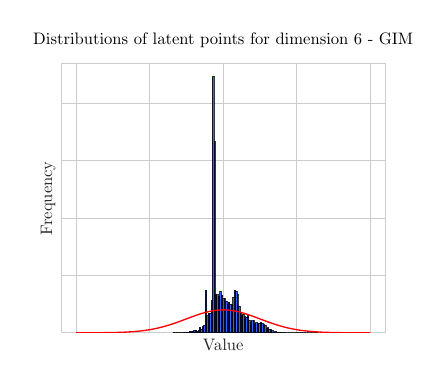
\begin{tikzpicture}[scale=0.6]

\definecolor{blue262255}{RGB}{2,62,255}
\definecolor{darkslategray38}{RGB}{38,38,38}
\definecolor{lightgray204}{RGB}{204,204,204}

\begin{axis}[
axis line style={lightgray204},
tick align=outside,
title={Distributions of latent points for dimension 6 - GIM},
x grid style={lightgray204},
xlabel=\textcolor{darkslategray38}{Value},
xmajorgrids,
xmajorticks=false,
xmin=-4.4, xmax=4.4,
xtick style={color=darkslategray38},
y grid style={lightgray204},
ylabel=\textcolor{darkslategray38}{Frequency},
ymajorgrids,
ymajorticks=false,
ymin=0, ymax=4.68745499004489,
ytick style={color=darkslategray38}
]
\draw[draw=black,fill=blue262255,opacity=0.8,line width=0.48pt] (axis cs:-1.35178446769714,0) rectangle (axis cs:-1.31251561641693,0.00676913244527946);
\draw[draw=black,fill=blue262255,opacity=0.8,line width=0.48pt] (axis cs:-1.31251549720764,0) rectangle (axis cs:-1.27324664592743,0.00338456622263973);
\draw[draw=black,fill=blue262255,opacity=0.8,line width=0.48pt] (axis cs:-1.27324676513672,0) rectangle (axis cs:-1.23397791385651,0);
\draw[draw=black,fill=blue262255,opacity=0.8,line width=0.48pt] (axis cs:-1.23397779464722,0) rectangle (axis cs:-1.194708943367,0);
\draw[draw=black,fill=blue262255,opacity=0.8,line width=0.48pt] (axis cs:-1.19470906257629,0) rectangle (axis cs:-1.15544021129608,0.00338456622263973);
\draw[draw=black,fill=blue262255,opacity=0.8,line width=0.48pt] (axis cs:-1.15544009208679,0) rectangle (axis cs:-1.11617136001587,0);
\draw[draw=black,fill=blue262255,opacity=0.8,line width=0.48pt] (axis cs:-1.11617136001587,0) rectangle (axis cs:-1.07690250873566,0);
\draw[draw=black,fill=blue262255,opacity=0.8,line width=0.48pt] (axis cs:-1.07690262794495,0) rectangle (axis cs:-1.03763377666473,0.0101536986679192);
\draw[draw=black,fill=blue262255,opacity=0.8,line width=0.48pt] (axis cs:-1.03763365745544,0) rectangle (axis cs:-0.998364806175232,0.0101536986679192);
\draw[draw=black,fill=blue262255,opacity=0.8,line width=0.48pt] (axis cs:-0.998364806175232,0) rectangle (axis cs:-0.95909595489502,0.00338456622263973);
\draw[draw=black,fill=blue262255,opacity=0.8,line width=0.48pt] (axis cs:-0.95909595489502,0) rectangle (axis cs:-0.919827103614807,0.0135382648905589);
\draw[draw=black,fill=blue262255,opacity=0.8,line width=0.48pt] (axis cs:-0.919827103614807,0) rectangle (axis cs:-0.880558252334595,0.0236919635584781);
\draw[draw=black,fill=blue262255,opacity=0.8,line width=0.48pt] (axis cs:-0.880558252334595,0) rectangle (axis cs:-0.841289401054382,0.0270765297811178);
\draw[draw=black,fill=blue262255,opacity=0.8,line width=0.48pt] (axis cs:-0.841289401054382,0) rectangle (axis cs:-0.802020668983459,0.0304611422395272);
\draw[draw=black,fill=blue262255,opacity=0.8,line width=0.48pt] (axis cs:-0.802020609378815,0) rectangle (axis cs:-0.762751758098602,0.0439993608943165);
\draw[draw=black,fill=blue262255,opacity=0.8,line width=0.48pt] (axis cs:-0.762751758098602,0) rectangle (axis cs:-0.72348290681839,0.0439993608943165);
\draw[draw=black,fill=blue262255,opacity=0.8,line width=0.48pt] (axis cs:-0.72348290681839,0) rectangle (axis cs:-0.684214055538177,0.0304610960037576);
\draw[draw=black,fill=blue262255,opacity=0.8,line width=0.48pt] (axis cs:-0.684214055538177,0) rectangle (axis cs:-0.644945204257965,0.0439993608943165);
\draw[draw=black,fill=blue262255,opacity=0.8,line width=0.48pt] (axis cs:-0.644945204257965,0) rectangle (axis cs:-0.605676352977753,0.101536986679192);
\draw[draw=black,fill=blue262255,opacity=0.8,line width=0.48pt] (axis cs:-0.605676293373108,0) rectangle (axis cs:-0.566407561302185,0.0643068558390019);
\draw[draw=black,fill=blue262255,opacity=0.8,line width=0.48pt] (axis cs:-0.566407561302185,0) rectangle (axis cs:-0.527138710021973,0.104921552901832);
\draw[draw=black,fill=blue262255,opacity=0.8,line width=0.48pt] (axis cs:-0.527138710021973,0) rectangle (axis cs:-0.48786985874176,0.131998082682949);
\draw[draw=black,fill=blue262255,opacity=0.8,line width=0.48pt] (axis cs:-0.48786985874176,0) rectangle (axis cs:-0.448601007461548,0.74460456898074);
\draw[draw=black,fill=blue262255,opacity=0.8,line width=0.48pt] (axis cs:-0.448601007461548,0) rectangle (axis cs:-0.409332156181335,0.294457484842373);
\draw[draw=black,fill=blue262255,opacity=0.8,line width=0.48pt] (axis cs:-0.409332185983658,0) rectangle (axis cs:-0.370063334703445,0.341841188486613);
\draw[draw=black,fill=blue262255,opacity=0.8,line width=0.48pt] (axis cs:-0.370063334703445,0) rectangle (axis cs:-0.330794483423233,0.341841188486613);
\draw[draw=black,fill=blue262255,opacity=0.8,line width=0.48pt] (axis cs:-0.330794513225555,0) rectangle (axis cs:-0.291525661945343,0.558453850563122);
\draw[draw=black,fill=blue262255,opacity=0.8,line width=0.48pt] (axis cs:-0.291525661945343,0) rectangle (axis cs:-0.252256810665131,4.4642428476618);
\draw[draw=black,fill=blue262255,opacity=0.8,line width=0.48pt] (axis cs:-0.252256810665131,0) rectangle (axis cs:-0.212987959384918,3.33041442685376);
\draw[draw=black,fill=blue262255,opacity=0.8,line width=0.48pt] (axis cs:-0.212987989187241,0) rectangle (axis cs:-0.173719137907028,0.67014436637911);
\draw[draw=black,fill=blue262255,opacity=0.8,line width=0.48pt] (axis cs:-0.173719137907028,0) rectangle (axis cs:-0.134450286626816,0.663374979637387);
\draw[draw=black,fill=blue262255,opacity=0.8,line width=0.48pt] (axis cs:-0.134450286626816,0) rectangle (axis cs:-0.0951814353466034,0.626144988788562);
\draw[draw=black,fill=blue262255,opacity=0.8,line width=0.48pt] (axis cs:-0.0951814576983452,0) rectangle (axis cs:-0.0559126064181328,0.71414367622147);
\draw[draw=black,fill=blue262255,opacity=0.8,line width=0.48pt] (axis cs:-0.0559126138687134,0) rectangle (axis cs:-0.016643762588501,0.656606034061446);
\draw[draw=black,fill=blue262255,opacity=0.8,line width=0.48pt] (axis cs:-0.016643775627017,0) rectangle (axis cs:0.0226250756531954,0.602452959087306);
\draw[draw=black,fill=blue262255,opacity=0.8,line width=0.48pt] (axis cs:0.0226250663399696,0) rectangle (axis cs:0.061893917620182,0.592299257529655);
\draw[draw=black,fill=blue262255,opacity=0.8,line width=0.48pt] (axis cs:0.0618939101696014,0) rectangle (axis cs:0.101162761449814,0.551684398962782);
\draw[draw=black,fill=blue262255,opacity=0.8,line width=0.48pt] (axis cs:0.101162746548653,0) rectangle (axis cs:0.140431597828865,0.494146762261142);
\draw[draw=black,fill=blue262255,opacity=0.8,line width=0.48pt] (axis cs:0.140431582927704,0) rectangle (axis cs:0.179700434207916,0.534761666100502);
\draw[draw=black,fill=blue262255,opacity=0.8,line width=0.48pt] (axis cs:0.179700434207916,0) rectangle (axis cs:0.218969285488129,0.50091599103085);
\draw[draw=black,fill=blue262255,opacity=0.8,line width=0.48pt] (axis cs:0.218969255685806,0) rectangle (axis cs:0.258238106966019,0.50091599103085);
\draw[draw=black,fill=blue262255,opacity=0.8,line width=0.48pt] (axis cs:0.258238106966019,0) rectangle (axis cs:0.297506958246231,0.61937561874307);
\draw[draw=black,fill=blue262255,opacity=0.8,line width=0.48pt] (axis cs:0.297506958246231,0) rectangle (axis cs:0.336775809526443,0.737835436535461);
\draw[draw=black,fill=blue262255,opacity=0.8,line width=0.48pt] (axis cs:0.336775779724121,0) rectangle (axis cs:0.376044631004333,0.727682290127704);
\draw[draw=black,fill=blue262255,opacity=0.8,line width=0.48pt] (axis cs:0.376044631004333,0) rectangle (axis cs:0.415313482284546,0.663374979637387);
\draw[draw=black,fill=blue262255,opacity=0.8,line width=0.48pt] (axis cs:0.415313482284546,0) rectangle (axis cs:0.454582333564758,0.460301355615664);
\draw[draw=black,fill=blue262255,opacity=0.8,line width=0.48pt] (axis cs:0.454582303762436,0) rectangle (axis cs:0.493851155042648,0.355379453377171);
\draw[draw=black,fill=blue262255,opacity=0.8,line width=0.48pt] (axis cs:0.493851125240326,0) rectangle (axis cs:0.533119976520538,0.311380328798832);
\draw[draw=black,fill=blue262255,opacity=0.8,line width=0.48pt] (axis cs:0.533119976520538,0) rectangle (axis cs:0.572388827800751,0.321533791150774);
\draw[draw=black,fill=blue262255,opacity=0.8,line width=0.48pt] (axis cs:0.572388827800751,0) rectangle (axis cs:0.611657679080963,0.277534430256458);
\draw[draw=black,fill=blue262255,opacity=0.8,line width=0.48pt] (axis cs:0.611657679080963,0) rectangle (axis cs:0.650926530361176,0.270765297811178);
\draw[draw=black,fill=blue262255,opacity=0.8,line width=0.48pt] (axis cs:0.650926530361176,0) rectangle (axis cs:0.690195381641388,0.294457261369656);
\draw[draw=black,fill=blue262255,opacity=0.8,line width=0.48pt] (axis cs:0.690195441246033,0) rectangle (axis cs:0.729464173316956,0.223381709756533);
\draw[draw=black,fill=blue262255,opacity=0.8,line width=0.48pt] (axis cs:0.729464173316956,0) rectangle (axis cs:0.768733024597168,0.189535708467825);
\draw[draw=black,fill=blue262255,opacity=0.8,line width=0.48pt] (axis cs:0.768733024597168,0) rectangle (axis cs:0.80800187587738,0.213227672026303);
\draw[draw=black,fill=blue262255,opacity=0.8,line width=0.48pt] (axis cs:0.80800187587738,0) rectangle (axis cs:0.847270727157593,0.209843105803663);
\draw[draw=black,fill=blue262255,opacity=0.8,line width=0.48pt] (axis cs:0.847270727157593,0) rectangle (axis cs:0.886539578437805,0.169228311131986);
\draw[draw=black,fill=blue262255,opacity=0.8,line width=0.48pt] (axis cs:0.886539578437805,0) rectangle (axis cs:0.925808429718018,0.175997443577266);
\draw[draw=black,fill=blue262255,opacity=0.8,line width=0.48pt] (axis cs:0.925808429718018,0) rectangle (axis cs:0.96507716178894,0.159074853917531);
\draw[draw=black,fill=blue262255,opacity=0.8,line width=0.48pt] (axis cs:0.96507716178894,0) rectangle (axis cs:1.00434613227844,0.165843493182032);
\draw[draw=black,fill=blue262255,opacity=0.8,line width=0.48pt] (axis cs:1.00434613227844,0) rectangle (axis cs:1.04361498355865,0.186151142245185);
\draw[draw=black,fill=blue262255,opacity=0.8,line width=0.48pt] (axis cs:1.04361498355865,0) rectangle (axis cs:1.08288371562958,0.165844248366269);
\draw[draw=black,fill=blue262255,opacity=0.8,line width=0.48pt] (axis cs:1.08288359642029,0) rectangle (axis cs:1.1221524477005,0.152305480018788);
\draw[draw=black,fill=blue262255,opacity=0.8,line width=0.48pt] (axis cs:1.12215256690979,0) rectangle (axis cs:1.16142141819,0.131998082682949);
\draw[draw=black,fill=blue262255,opacity=0.8,line width=0.48pt] (axis cs:1.16142129898071,0) rectangle (axis cs:1.20069015026093,0.0778450231207137);
\draw[draw=black,fill=blue262255,opacity=0.8,line width=0.48pt] (axis cs:1.20069026947021,0) rectangle (axis cs:1.23995912075043,0.0913832880112727);
\draw[draw=black,fill=blue262255,opacity=0.8,line width=0.48pt] (axis cs:1.23995900154114,0) rectangle (axis cs:1.27922785282135,0.0643067582301548);
\draw[draw=black,fill=blue262255,opacity=0.8,line width=0.48pt] (axis cs:1.27922797203064,0) rectangle (axis cs:1.31849682331085,0.0541530595622357);
\draw[draw=black,fill=blue262255,opacity=0.8,line width=0.48pt] (axis cs:1.31849670410156,0) rectangle (axis cs:1.35776555538177,0.037230228449037);
\draw[draw=black,fill=blue262255,opacity=0.8,line width=0.48pt] (axis cs:1.35776567459106,0) rectangle (axis cs:1.39703452587128,0.0101536986679192);
\draw[draw=black,fill=blue262255,opacity=0.8,line width=0.48pt] (axis cs:1.39703440666199,0) rectangle (axis cs:1.4363032579422,0.0169228311131986);
\draw[draw=black,fill=blue262255,opacity=0.8,line width=0.48pt] (axis cs:1.43630337715149,0) rectangle (axis cs:1.4755722284317,0.0101536986679192);
\draw[draw=black,fill=blue262255,opacity=0.8,line width=0.48pt] (axis cs:1.4755722284317,0) rectangle (axis cs:1.51484096050262,0.0101537294918124);
\draw[draw=black,fill=blue262255,opacity=0.8,line width=0.48pt] (axis cs:1.51484084129333,0) rectangle (axis cs:1.55410969257355,0);
\draw[draw=black,fill=blue262255,opacity=0.8,line width=0.48pt] (axis cs:1.55410981178284,0) rectangle (axis cs:1.59337866306305,0.0101536986679192);
\draw[draw=black,fill=blue262255,opacity=0.8,line width=0.48pt] (axis cs:1.59337854385376,0) rectangle (axis cs:1.63264739513397,0.00338456622263973);
\draw[draw=black,fill=blue262255,opacity=0.8,line width=0.48pt] (axis cs:1.63264751434326,0) rectangle (axis cs:1.67191636562347,0.00676913244527946);
\draw[draw=black,fill=blue262255,opacity=0.8,line width=0.48pt] (axis cs:1.67191624641418,0) rectangle (axis cs:1.7111850976944,0);
\draw[draw=black,fill=blue262255,opacity=0.8,line width=0.48pt] (axis cs:1.71118521690369,0) rectangle (axis cs:1.7504540681839,0);
\draw[draw=black,fill=blue262255,opacity=0.8,line width=0.48pt] (axis cs:1.75045394897461,0) rectangle (axis cs:1.78972280025482,0);
\draw[draw=black,fill=blue262255,opacity=0.8,line width=0.48pt] (axis cs:1.78972291946411,0) rectangle (axis cs:1.82899177074432,0);
\draw[draw=black,fill=blue262255,opacity=0.8,line width=0.48pt] (axis cs:1.82899165153503,0) rectangle (axis cs:1.86826050281525,0);
\draw[draw=black,fill=blue262255,opacity=0.8,line width=0.48pt] (axis cs:1.86826062202454,0) rectangle (axis cs:1.90752947330475,0);
\draw[draw=black,fill=blue262255,opacity=0.8,line width=0.48pt] (axis cs:1.90752947330475,0) rectangle (axis cs:1.94679820537567,0);
\draw[draw=black,fill=blue262255,opacity=0.8,line width=0.48pt] (axis cs:1.94679808616638,0) rectangle (axis cs:1.98606693744659,0);
\draw[draw=black,fill=blue262255,opacity=0.8,line width=0.48pt] (axis cs:1.98606705665588,0) rectangle (axis cs:2.02533602714539,0.00338455594807103);
\draw[draw=black,fill=blue262255,opacity=0.8,line width=0.48pt] (axis cs:2.02533626556396,0) rectangle (axis cs:2.06460499763489,0);
\draw[draw=black,fill=blue262255,opacity=0.8,line width=0.48pt] (axis cs:2.06460475921631,0) rectangle (axis cs:2.10387372970581,0);
\draw[draw=black,fill=blue262255,opacity=0.8,line width=0.48pt] (axis cs:2.10387372970581,0) rectangle (axis cs:2.14314246177673,0.0033845764972708);
\draw[draw=black,fill=blue262255,opacity=0.8,line width=0.48pt] (axis cs:2.14314270019531,0) rectangle (axis cs:2.18241143226624,0);
\draw[draw=black,fill=blue262255,opacity=0.8,line width=0.48pt] (axis cs:2.18241119384766,0) rectangle (axis cs:2.22168016433716,0);
\draw[draw=black,fill=blue262255,opacity=0.8,line width=0.48pt] (axis cs:2.22168016433716,0) rectangle (axis cs:2.26094889640808,0);
\draw[draw=black,fill=blue262255,opacity=0.8,line width=0.48pt] (axis cs:2.26094889640808,0) rectangle (axis cs:2.30021786689758,0);
\draw[draw=black,fill=blue262255,opacity=0.8,line width=0.48pt] (axis cs:2.30021810531616,0) rectangle (axis cs:2.33948683738708,0);
\draw[draw=black,fill=blue262255,opacity=0.8,line width=0.48pt] (axis cs:2.33948659896851,0) rectangle (axis cs:2.37875556945801,0);
\draw[draw=black,fill=blue262255,opacity=0.8,line width=0.48pt] (axis cs:2.37875556945801,0) rectangle (axis cs:2.41802430152893,0);
\draw[draw=black,fill=blue262255,opacity=0.8,line width=0.48pt] (axis cs:2.41802430152893,0) rectangle (axis cs:2.45729327201843,0);
\draw[draw=black,fill=blue262255,opacity=0.8,line width=0.48pt] (axis cs:2.45729351043701,0) rectangle (axis cs:2.49656224250793,0);
\draw[draw=black,fill=blue262255,opacity=0.8,line width=0.48pt] (axis cs:2.49656200408936,0) rectangle (axis cs:2.53583097457886,0);
\draw[draw=black,fill=blue262255,opacity=0.8,line width=0.48pt] (axis cs:2.53583097457886,0) rectangle (axis cs:2.57509970664978,0.0033845764972708);
\addplot [thick, red]
table {%
-4 0.000133830225764885
-3.99199199199199 0.000138182046410498
-3.98398398398398 0.000142666228042307
-3.97597597597598 0.000147286481503254
-3.96796796796797 0.000152046611333821
-3.95995995995996 0.000156950517814782
-3.95195195195195 0.00016200219904485
-3.94394394394394 0.00016720575305353
-3.93593593593594 0.000172565379949496
-3.92792792792793 0.00017808538410479
-3.91991991991992 0.000183770176375138
-3.91191191191191 0.000189624276356684
-3.9039039039039 0.000195652314679408
-3.8958958958959 0.000201859035337517
-3.88788788788789 0.000208249298057069
-3.87987987987988 0.000214828080701088
-3.87187187187187 0.000221600481712426
-3.86386386386386 0.0002285717225946
-3.85585585585586 0.000235747150430845
-3.84784784784785 0.000243132240441603
-3.83983983983984 0.000250732598580649
-3.83183183183183 0.000258553964170059
-3.82382382382382 0.000266602212574213
-3.81581581581582 0.000274883357912987
-3.80780780780781 0.000283403555814325
-3.7997997997998 0.000292169106206322
-3.79179179179179 0.000301186456148957
-3.78378378378378 0.0003104622027056
-3.77577577577578 0.000320003095854415
-3.76776776776777 0.000329816041439723
-3.75975975975976 0.000339908104163431
-3.75175175175175 0.00035028651061658
-3.74374374374374 0.000360958652351047
-3.73573573573574 0.000371932088991451
-3.72772772772773 0.000383214551387261
-3.71971971971972 0.000394813944805093
-3.71171171171171 0.000406738352161197
-3.7037037037037 0.000418996037294058
-3.6956956956957 0.00043159544827708
-3.68768768768769 0.00044454522077123
-3.67967967967968 0.000457854181417586
-3.67167167167167 0.000471531351269624
-3.66366366366366 0.000485585949265103
-3.65565565565566 0.000500027395737409
-3.64764764764765 0.000514865315966112
-3.63963963963964 0.000530109543766577
-3.63163163163163 0.000545770125118336
-3.62362362362362 0.000561857321831991
-3.61561561561562 0.00057838161525435
-3.60760760760761 0.000595353710011453
-3.5995995995996 0.000612784537789192
-3.59159159159159 0.000630685261151105
-3.58358358358358 0.000649067277392973
-3.57557557557558 0.000667942222433796
-3.56756756756757 0.000687321974742665
-3.55955955955956 0.000707218659301081
-3.55155155155155 0.000727644651600166
-3.54354354354354 0.000748612581672245
-3.53553553553554 0.000770135338156225
-3.52752752752753 0.000792226072396121
-3.51951951951952 0.00081489820257214
-3.51151151151151 0.000838165417863603
-3.5035035035035 0.000862041682643007
-3.4954954954955 0.000886541240700502
-3.48748748748749 0.00091167861949796
-3.47947947947948 0.000937468634451866
-3.47147147147147 0.000963926393244149
-3.46346346346346 0.000991067300160059
-3.45545545545546 0.0010189070604522
-3.44744744744745 0.00104746168472971
-3.43943943943944 0.0010767474933716
-3.43143143143143 0.00110678112096323
-3.42342342342342 0.00113757952075483
-3.41541541541542 0.00116915996914087
-3.40740740740741 0.00120154007015926
-3.3993993993994 0.00123473776000907
-3.39139139139139 0.00126877131158549
-3.38338338338338 0.00130365933903088
-3.37537537537538 0.00133942080230046
-3.36736736736737 0.00137607501174126
-3.35935935935936 0.001413641632683
-3.35135135135135 0.00145214069003938
-3.34334334334334 0.0014915925729182
-3.33533533533534 0.00153201803923895
-3.32732732732733 0.00157343822035606
-3.31931931931932 0.00161587462568624
-3.31131131131131 0.00165934914733831
-3.3033033033033 0.00170388406474362
-3.2952952952953 0.00174950204928538
-3.28728728728729 0.00179622616892505
-3.27927927927928 0.00184407989282385
-3.27127127127127 0.00189308709595757
-3.26326326326326 0.00194327206372255
-3.25525525525526 0.00199465949653091
-3.24724724724725 0.00204727451439301
-3.23923923923924 0.00210114266148476
-3.23123123123123 0.00215628991069791
-3.22322322322322 0.00221274266817093
-3.21521521521522 0.00227052777779815
-3.20720720720721 0.00232967252571501
-3.1991991991992 0.00239020464475689
-3.19119119119119 0.00245215231888918
-3.18318318318318 0.00251554418760605
-3.17517517517518 0.00258040935029545
-3.16716716716717 0.00264677737056774
-3.15915915915916 0.00271467828054534
-3.15115115115115 0.00278414258511061
-3.14314314314314 0.00285520126610952
-3.13513513513514 0.00292788578650791
-3.12712712712713 0.00300222809449793
-3.11911911911912 0.00307826062755151
-3.11111111111111 0.00315601631641804
-3.1031031031031 0.00323552858906328
-3.0950950950951 0.00331683137454643
-3.08708708708709 0.00339995910683238
-3.07907907907908 0.00348494672853595
-3.07107107107107 0.00357182969459489
-3.06306306306306 0.00366064397586864
-3.05505505505506 0.00375142606265932
-3.04704704704705 0.00384421296815189
-3.03903903903904 0.00393904223176991
-3.03103103103103 0.00403595192244368
-3.02302302302302 0.0041349806417872
-3.01501501501502 0.00423616752718052
-3.00700700700701 0.00433955225475399
-2.998998998999 0.00444517504227068
-2.99099099099099 0.00455307665190355
-2.98298298298298 0.00466329839290368
-2.97497497497497 0.00477588212415564
-2.96696696696697 0.00489087025661667
-2.95895895895896 0.00500830575563558
-2.95095095095095 0.00512823214314763
-2.94294294294294 0.00525069349974172
-2.93493493493493 0.00537573446659573
-2.92692692692693 0.00550340024727644
-2.91891891891892 0.00563373660939975
-2.91091091091091 0.0057667898861475
-2.9029029029029 0.00590260697763674
-2.89489489489489 0.00604123535213746
-2.88688688688689 0.00618272304713484
-2.87887887887888 0.00632711867023164
-2.87087087087087 0.00647447139988703
-2.86286286286286 0.00662483098598741
-2.85485485485485 0.0067782477502453
-2.84684684684685 0.0069347725864219
-2.83883883883884 0.00709445696036946
-2.83083083083083 0.00725735290988893
-2.82282282282282 0.00742351304439893
-2.81481481481481 0.00759299054441176
-2.80680680680681 0.0077658391608121
-2.7987987987988 0.00794211321393437
-2.79079079079079 0.00812186759243432
-2.78278278278278 0.00830515775195071
-2.77477477477477 0.00849203971355293
-2.76676676676677 0.00868257006197001
-2.75875875875876 0.00887680594359712
-2.75075075075075 0.00907480506427511
-2.74274274274274 0.00927662568683898
-2.73473473473473 0.00948232662843099
-2.72672672672673 0.00969196725757422
-2.71871871871872 0.00990560749100246
-2.71071071071071 0.0101233077902421
-2.7027027027027 0.0103451291579421
-2.69469469469469 0.0105711331339476
-2.68668668668669 0.0108013817911136
-2.67867867867868 0.011035937730854
-2.67067067067067 0.0112748640784219
-2.66266266266266 0.0115182244779185
-2.65465465465465 0.0117660830870247
-2.64664664664665 0.0120185045714526
-2.63863863863864 0.0122755540991133
-2.63063063063063 0.0125372973339956
-2.62262262262262 0.0128038004297541
-2.61461461461461 0.0130751300230007
-2.60660660660661 0.0133513532262973
-2.5985985985986 0.0136325376208454
-2.59059059059059 0.0139187512488692
-2.58258258258258 0.014210062605689
-2.57457457457457 0.0145065406314803
-2.56656656656657 0.0148082547027168
-2.55855855855856 0.0151152746232934
-2.55055055055055 0.0154276706153247
-2.54254254254254 0.0157455133096184
-2.53453453453453 0.0160688737358178
-2.52652652652653 0.016397823312213
-2.51851851851852 0.0167324338352151
-2.51051051051051 0.0170727774684938
-2.5025025025025 0.0174189267317727
-2.49449449449449 0.0177709544892815
-2.48648648648649 0.0181289339378627
-2.47847847847848 0.0184929385947284
-2.47047047047047 0.0188630422848682
-2.46246246246246 0.0192393191281025
-2.45445445445445 0.0196218435257817
-2.44644644644645 0.0200106901471285
-2.43843843843844 0.020405933915221
-2.43043043043043 0.0208076499926159
-2.42242242242242 0.0212159137666093
-2.41441441441441 0.0216308008341344
-2.40640640640641 0.0220523869862944
-2.3983983983984 0.0224807481925294
-2.39039039039039 0.022915960584417
-2.38238238238238 0.0233581004391047
-2.37437437437437 0.023807244162374
-2.36636636636637 0.0242634682713357
-2.35835835835836 0.0247268493767558
-2.35035035035035 0.0251974641650118
-2.34234234234234 0.0256753893796796
-2.33433433433433 0.0261607018027501
-2.32632632632633 0.0266534782354775
-2.31831831831832 0.0271537954788581
-2.31031031031031 0.0276617303137407
-2.3023023023023 0.0281773594805703
-2.29429429429429 0.0287007596587648
-2.28628628628629 0.0292320074457259
-2.27827827827828 0.029771179335487
-2.27027027027027 0.0303183516969979
-2.26226226226226 0.0308736007520491
-2.25425425425425 0.0314370025528369
-2.24624624624625 0.0320086329591723
-2.23823823823824 0.0325885676153351
-2.23023023023023 0.0331768819265761
-2.22222222222222 0.0337736510352706
-2.21421421421421 0.0343789497967251
-2.20620620620621 0.0349928527546413
-2.1981981981982 0.0356154341162401
-2.19019019019019 0.0362467677270497
-2.18218218218218 0.0368869270453615
-2.17417417417417 0.0375359851163567
-2.16616616616617 0.03819401454591
-2.15815815815816 0.0388610874740724
-2.15015015015015 0.03953727554824
-2.14214214214214 0.0402226498960119
-2.13413413413413 0.0409172810977437
-2.12612612612613 0.0416212391588003
-2.11811811811812 0.0423345934815158
-2.11011011011011 0.0430574128368641
-2.1021021021021 0.043789765335848
-2.09409409409409 0.0445317184006117
-2.08608608608609 0.0452833387352837
-2.07807807807808 0.0460446922965577
-2.07007007007007 0.0468158442640166
-2.06206206206206 0.0475968590102091
-2.05405405405405 0.0483878000704834
-2.04604604604605 0.0491887301125894
-2.03803803803804 0.0499997109060533
-2.03003003003003 0.0508208032913361
-2.02202202202202 0.0516520671487823
-2.01401401401401 0.0524935613673682
-2.00600600600601 0.053345343813258
-1.997997997998 0.0542074712981785
-1.98998998998999 0.0550799995476186
-1.98198198198198 0.0559629831688668
-1.97397397397397 0.0568564756188931
-1.96596596596597 0.0577605291720876
-1.95795795795796 0.0586751948878651
-1.94994994994995 0.0596005225781457
-1.94194194194194 0.0605365607747232
-1.93393393393393 0.0614833566965309
-1.92592592592593 0.062440956216817
-1.91791791791792 0.06340940383024
-1.90990990990991 0.0643887426198963
-1.9019019019019 0.0653790142242912
-1.89389389389389 0.0663802588042656
-1.88588588588589 0.0673925150098903
-1.87787787787788 0.0684158199473405
-1.86986986986987 0.0694502091457625
-1.86186186186186 0.0704957165241465
-1.85385385385385 0.0715523743582165
-1.84584584584585 0.0726202132473521
-1.83783783783784 0.0736992620815557
-1.82982982982983 0.0747895480084762
-1.82182182182182 0.0758910964005057
-1.81381381381381 0.0770039308219614
-1.80580580580581 0.0781280729963669
-1.7977977977978 0.0792635427738473
-1.78978978978979 0.0804103580986525
-1.78178178178178 0.0815685349768227
-1.77377377377377 0.0827380874440109
-1.76576576576577 0.0839190275334777
-1.75775775775776 0.0851113652442723
-1.74974974974975 0.086315108509615
-1.74174174174174 0.0875302631654975
-1.73373373373373 0.0887568329195139
-1.72572572572573 0.0899948193199405
-1.71771771771772 0.0912442217250772
-1.70970970970971 0.0925050372728685
-1.7017017017017 0.0937772608508177
-1.69369369369369 0.0950608850662112
-1.68568568568569 0.0963559002166691
-1.67767767767768 0.0976622942610365
-1.66966966966967 0.0989800527906321
-1.66166166166166 0.100309159000872
-1.65365365365365 0.10164959366328
-1.64564564564565 0.103001335097907
-1.63763763763764 0.10436435914617
-1.62962962962963 0.105738639144131
-1.62162162162162 0.107124145896225
-1.61361361361361 0.108520847649465
-1.60560560560561 0.10992871006813
-1.5975975975976 0.111347696208955
-1.58958958958959 0.112777766496842
-1.58158158158158 0.114218878701105
-1.57357357357357 0.115670987912262
-1.56556556556557 0.117134046519405
-1.55755755755756 0.11860800418814
-1.54954954954955 0.120092807839133
-1.54154154154154 0.121588401627275
-1.53353353353353 0.123094726921466
-1.52552552552553 0.124611722285057
-1.51751751751752 0.12613932345695
-1.50950950950951 0.127677463333369
-1.5015015015015 0.129226071950339
-1.49349349349349 0.130785076466857
-1.48548548548549 0.132354401148798
-1.47747747747748 0.133933967353555
-1.46946946946947 0.13552369351543
-1.46146146146146 0.137123495131801
-1.45345345345345 0.13873328475006
-1.44544544544545 0.140352971955359
-1.43743743743744 0.141982463359159
-1.42942942942943 0.143621662588612
-1.42142142142142 0.14527047027677
-1.41341341341341 0.146928784053658
-1.40540540540541 0.148596498538208
-1.3973973973974 0.150273505331067
-1.38938938938939 0.151959693008306
-1.38138138138138 0.153654947116025
-1.37337337337337 0.155359150165875
-1.36536536536537 0.157072181631514
-1.35735735735736 0.158793917945997
-1.34934934934935 0.160524232500121
-1.34134134134134 0.16226299564173
-1.33333333333333 0.164010074675994
-1.32532532532533 0.165765333866673
-1.31731731731732 0.167528634438376
-1.30930930930931 0.169299834579821
-1.3013013013013 0.17107878944811
-1.29329329329329 0.172865351174024
-1.28528528528529 0.174659368868355
-1.27727727727728 0.176460688629273
-1.26926926926927 0.178269153550739
-1.26126126126126 0.180084603731981
-1.25325325325325 0.181906876288021
-1.24524524524525 0.183735805361283
-1.23723723723724 0.185571222134271
-1.22922922922923 0.187412954843324
-1.22122122122122 0.18926082879347
-1.21321321321321 0.191114666374361
-1.20520520520521 0.192974287077311
-1.1971971971972 0.194839507513435
-1.18918918918919 0.19671014143289
-1.18118118118118 0.198585999745227
-1.17317317317317 0.200466890540856
-1.16516516516517 0.202352619113618
-1.15715715715716 0.204242987984477
-1.14914914914915 0.206137796926331
-1.14114114114114 0.208036842989938
-1.13313313313313 0.209939920530956
-1.12512512512513 0.21184682123811
-1.11711711711712 0.21375733416247
-1.10910910910911 0.215671245747847
-1.1011011011011 0.217588339862305
-1.09309309309309 0.219508397830784
-1.08508508508509 0.221431198468836
-1.07707707707708 0.223356518117463
-1.06906906906907 0.225284130679063
-1.06106106106106 0.22721380765447
-1.05305305305305 0.229145318181096
-1.04504504504505 0.231078429072154
-1.03703703703704 0.233012904856966
-1.02902902902903 0.234948507822352
-1.02102102102102 0.236884998055083
-1.01301301301301 0.238822133485401
-1.00500500500501 0.24075966993159
-0.996996996996997 0.242697361145593
-0.988988988988989 0.244634958859672
-0.980980980980981 0.246572212834085
-0.972972972972973 0.248508870905785
-0.964964964964965 0.250444679038131
-0.956956956956957 0.252379381371581
-0.948948948948949 0.254312720275385
-0.940940940940941 0.256244436400228
-0.932932932932933 0.258174268731856
-0.924924924924925 0.260101954645624
-0.916916916916917 0.262027229961987
-0.908908908908909 0.263949829002911
-0.900900900900901 0.265869484649172
-0.892892892892893 0.267785928398552
-0.884884884884885 0.269698890424904
-0.876876876876877 0.271608099638066
-0.868868868868869 0.273513283744617
-0.860860860860861 0.275414169309444
-0.852852852852853 0.277310481818125
-0.844844844844845 0.279201945740075
-0.836836836836837 0.281088284592474
-0.828828828828829 0.28296922100493
-0.820820820820821 0.284844476784867
-0.812812812812813 0.286713772983616
-0.804804804804805 0.288576829963198
-0.796796796796797 0.290433367463758
-0.788788788788789 0.292283104671645
-0.780780780780781 0.294125760288111
-0.772772772772773 0.295961052598604
-0.764764764764765 0.29778869954263
-0.756756756756757 0.299608418784177
-0.748748748748749 0.301419927782648
-0.740740740740741 0.303222943864308
-0.732732732732733 0.305017184294205
-0.724724724724725 0.306802366348536
-0.716716716716717 0.308578207387456
-0.708708708708709 0.310344424928268
-0.700700700700701 0.312100736719007
-0.692692692692693 0.313846860812361
-0.684684684684685 0.31558251563992
-0.676676676676677 0.317307420086723
-0.668668668668669 0.319021293566066
-0.660660660660661 0.320723856094559
-0.652652652652653 0.322414828367396
-0.644644644644645 0.324093931833804
-0.636636636636636 0.325760888772662
-0.628628628628629 0.327415422368237
-0.620620620620621 0.329057256786028
-0.612612612612613 0.330686117248681
-0.604604604604605 0.33230173011195
-0.596596596596596 0.333903822940662
-0.588588588588589 0.335492124584683
-0.580580580580581 0.337066365254824
-0.572572572572573 0.338626276598684
-0.564564564564565 0.340171591776383
-0.556556556556556 0.341702045536168
-0.548548548548549 0.343217374289848
-0.54054054054054 0.344717316188045
-0.532532532532533 0.346201611195215
-0.524524524524525 0.347670001164422
-0.516516516516516 0.349122229911825
-0.508508508508509 0.350558043290856
-0.5005005005005 0.351977189266054
-0.492492492492492 0.353379417986526
-0.484484484484485 0.354764481859011
-0.476476476476476 0.356132135620502
-0.468468468468469 0.357482136410418
-0.46046046046046 0.358814243842273
-0.452452452452452 0.360128220074839
-0.444444444444445 0.361423829882744
-0.436436436436436 0.362700840726495
-0.428428428428429 0.363959022821904
-0.42042042042042 0.365198149208855
-0.412412412412412 0.366417995819425
-0.404404404404405 0.3676183415453
-0.396396396396396 0.368798968304465
-0.388388388388389 0.369959661107154
-0.38038038038038 0.37110020812101
-0.372372372372372 0.372220400735444
-0.364364364364365 0.373320033625156
-0.356356356356356 0.374398904812801
-0.348348348348348 0.375456815730761
-0.34034034034034 0.376493571282005
-0.332332332332332 0.377508979900006
-0.324324324324325 0.378502853607702
-0.316316316316316 0.379475008075448
-0.308308308308308 0.380425262677969
-0.3003003003003 0.38135344055026
-0.292292292292292 0.382259368642425
-0.284284284284285 0.38314287777343
-0.276276276276276 0.384003802683735
-0.268268268268268 0.3848419820868
-0.26026026026026 0.385657258719425
-0.252252252252252 0.386449479390916
-0.244244244244244 0.387218495031049
-0.236236236236236 0.387964160736805
-0.228228228228228 0.38868633581787
-0.22022022022022 0.389384883840873
-0.212212212212212 0.390059672672329
-0.204204204204204 0.390710574520297
-0.196196196196196 0.391337465974705
-0.188188188188188 0.39194022804635
-0.18018018018018 0.392518746204527
-0.172172172172172 0.393072910413305
-0.164164164164164 0.393602615166401
-0.156156156156156 0.394107759520658
-0.148148148148148 0.394588247128102
-0.14014014014014 0.395043986266573
-0.132132132132132 0.3954748898689
-0.124124124124124 0.395880875550626
-0.116116116116116 0.396261865636259
-0.108108108108108 0.396617787184037
-0.1001001001001 0.396948572009207
-0.0920920920920922 0.397254156705792
-0.084084084084084 0.397534482666846
-0.0760760760760761 0.39778949610319
-0.0680680680680683 0.39801914806061
-0.06006006006006 0.398223394435522
-0.0520520520520522 0.398402195989086
-0.0440440440440439 0.398555518359772
-0.0360360360360361 0.398683332074364
-0.0280280280280278 0.398785612557403
-0.02002002002002 0.398862340139061
-0.0120120120120122 0.398913500061449
-0.00400400400400391 0.398939082483343
0.00400400400400436 0.398939082483343
0.0120120120120122 0.398913500061449
0.02002002002002 0.398862340139061
0.0280280280280278 0.398785612557403
0.0360360360360357 0.398683332074364
0.0440440440440444 0.398555518359772
0.0520520520520522 0.398402195989086
0.06006006006006 0.398223394435522
0.0680680680680679 0.39801914806061
0.0760760760760757 0.39778949610319
0.0840840840840844 0.397534482666846
0.0920920920920922 0.397254156705792
0.1001001001001 0.396948572009207
0.108108108108108 0.396617787184037
0.116116116116116 0.396261865636259
0.124124124124124 0.395880875550626
0.132132132132132 0.3954748898689
0.14014014014014 0.395043986266573
0.148148148148148 0.394588247128102
0.156156156156156 0.394107759520658
0.164164164164164 0.393602615166401
0.172172172172172 0.393072910413305
0.18018018018018 0.392518746204527
0.188188188188188 0.39194022804635
0.196196196196196 0.391337465974705
0.204204204204204 0.390710574520297
0.212212212212212 0.390059672672329
0.22022022022022 0.389384883840873
0.228228228228228 0.388686335817871
0.236236236236236 0.387964160736805
0.244244244244245 0.387218495031049
0.252252252252252 0.386449479390916
0.26026026026026 0.385657258719425
0.268268268268268 0.3848419820868
0.276276276276276 0.384003802683735
0.284284284284285 0.38314287777343
0.292292292292292 0.382259368642425
0.3003003003003 0.38135344055026
0.308308308308308 0.380425262677969
0.316316316316316 0.379475008075448
0.324324324324325 0.378502853607702
0.332332332332332 0.377508979900006
0.34034034034034 0.376493571282005
0.348348348348348 0.375456815730762
0.356356356356356 0.374398904812801
0.364364364364365 0.373320033625156
0.372372372372372 0.372220400735444
0.38038038038038 0.37110020812101
0.388388388388388 0.369959661107154
0.396396396396397 0.368798968304465
0.404404404404405 0.3676183415453
0.412412412412412 0.366417995819425
0.42042042042042 0.365198149208855
0.428428428428428 0.363959022821904
0.436436436436437 0.362700840726495
0.444444444444445 0.361423829882744
0.452452452452452 0.360128220074839
0.46046046046046 0.358814243842273
0.468468468468468 0.357482136410418
0.476476476476477 0.356132135620502
0.484484484484485 0.354764481859011
0.492492492492492 0.353379417986526
0.5005005005005 0.351977189266054
0.508508508508508 0.350558043290856
0.516516516516517 0.349122229911825
0.524524524524525 0.347670001164422
0.532532532532533 0.346201611195215
0.54054054054054 0.344717316188045
0.548548548548548 0.343217374289848
0.556556556556557 0.341702045536168
0.564564564564565 0.340171591776383
0.572572572572573 0.338626276598684
0.58058058058058 0.337066365254824
0.588588588588588 0.335492124584683
0.596596596596597 0.333903822940662
0.604604604604605 0.33230173011195
0.612612612612613 0.330686117248681
0.62062062062062 0.329057256786028
0.628628628628628 0.327415422368237
0.636636636636637 0.325760888772662
0.644644644644645 0.324093931833804
0.652652652652653 0.322414828367396
0.66066066066066 0.32072385609456
0.668668668668668 0.319021293566066
0.676676676676677 0.317307420086723
0.684684684684685 0.31558251563992
0.692692692692693 0.313846860812361
0.7007007007007 0.312100736719007
0.708708708708708 0.310344424928268
0.716716716716717 0.308578207387456
0.724724724724725 0.306802366348536
0.732732732732733 0.305017184294205
0.74074074074074 0.303222943864308
0.748748748748748 0.301419927782648
0.756756756756757 0.299608418784177
0.764764764764765 0.29778869954263
0.772772772772773 0.295961052598604
0.780780780780781 0.294125760288111
0.788788788788788 0.292283104671645
0.796796796796797 0.290433367463758
0.804804804804805 0.288576829963198
0.812812812812813 0.286713772983616
0.820820820820821 0.284844476784867
0.828828828828828 0.282969221004931
0.836836836836837 0.281088284592474
0.844844844844845 0.279201945740075
0.852852852852853 0.277310481818125
0.860860860860861 0.275414169309444
0.868868868868869 0.273513283744617
0.876876876876877 0.271608099638066
0.884884884884885 0.269698890424904
0.892892892892893 0.267785928398552
0.900900900900901 0.265869484649172
0.908908908908909 0.263949829002911
0.916916916916917 0.262027229961987
0.924924924924925 0.260101954645624
0.932932932932933 0.258174268731856
0.940940940940941 0.256244436400228
0.948948948948949 0.254312720275384
0.956956956956957 0.252379381371581
0.964964964964965 0.250444679038131
0.972972972972973 0.248508870905785
0.980980980980981 0.246572212834085
0.988988988988989 0.244634958859672
0.996996996996997 0.242697361145593
1.00500500500501 0.24075966993159
1.01301301301301 0.238822133485401
1.02102102102102 0.236884998055083
1.02902902902903 0.234948507822352
1.03703703703704 0.233012904856966
1.04504504504505 0.231078429072154
1.05305305305305 0.229145318181096
1.06106106106106 0.22721380765447
1.06906906906907 0.225284130679062
1.07707707707708 0.223356518117463
1.08508508508509 0.221431198468836
1.09309309309309 0.219508397830784
1.1011011011011 0.217588339862305
1.10910910910911 0.215671245747847
1.11711711711712 0.21375733416247
1.12512512512513 0.21184682123811
1.13313313313313 0.209939920530956
1.14114114114114 0.208036842989938
1.14914914914915 0.206137796926331
1.15715715715716 0.204242987984477
1.16516516516517 0.202352619113618
1.17317317317317 0.200466890540856
1.18118118118118 0.198585999745228
1.18918918918919 0.19671014143289
1.1971971971972 0.194839507513435
1.20520520520521 0.192974287077311
1.21321321321321 0.191114666374361
1.22122122122122 0.18926082879347
1.22922922922923 0.187412954843324
1.23723723723724 0.185571222134271
1.24524524524525 0.183735805361283
1.25325325325325 0.181906876288021
1.26126126126126 0.180084603731981
1.26926926926927 0.178269153550739
1.27727727727728 0.176460688629273
1.28528528528529 0.174659368868355
1.29329329329329 0.172865351174024
1.3013013013013 0.17107878944811
1.30930930930931 0.169299834579821
1.31731731731732 0.167528634438376
1.32532532532533 0.165765333866673
1.33333333333333 0.164010074675994
1.34134134134134 0.16226299564173
1.34934934934935 0.160524232500121
1.35735735735736 0.158793917945997
1.36536536536537 0.157072181631514
1.37337337337337 0.155359150165875
1.38138138138138 0.153654947116025
1.38938938938939 0.151959693008306
1.3973973973974 0.150273505331067
1.40540540540541 0.148596498538208
1.41341341341341 0.146928784053658
1.42142142142142 0.14527047027677
1.42942942942943 0.143621662588612
1.43743743743744 0.141982463359159
1.44544544544545 0.140352971955359
1.45345345345345 0.13873328475006
1.46146146146146 0.137123495131801
1.46946946946947 0.13552369351543
1.47747747747748 0.133933967353555
1.48548548548549 0.132354401148798
1.49349349349349 0.130785076466857
1.5015015015015 0.129226071950339
1.50950950950951 0.127677463333369
1.51751751751752 0.12613932345695
1.52552552552553 0.124611722285057
1.53353353353353 0.123094726921466
1.54154154154154 0.121588401627275
1.54954954954955 0.120092807839133
1.55755755755756 0.11860800418814
1.56556556556557 0.117134046519405
1.57357357357357 0.115670987912262
1.58158158158158 0.114218878701105
1.58958958958959 0.112777766496842
1.5975975975976 0.111347696208955
1.60560560560561 0.10992871006813
1.61361361361361 0.108520847649465
1.62162162162162 0.107124145896225
1.62962962962963 0.105738639144131
1.63763763763764 0.10436435914617
1.64564564564565 0.103001335097907
1.65365365365365 0.10164959366328
1.66166166166166 0.100309159000872
1.66966966966967 0.0989800527906321
1.67767767767768 0.0976622942610365
1.68568568568569 0.0963559002166692
1.69369369369369 0.0950608850662112
1.7017017017017 0.0937772608508176
1.70970970970971 0.0925050372728685
1.71771771771772 0.0912442217250772
1.72572572572573 0.0899948193199405
1.73373373373373 0.088756832919514
1.74174174174174 0.0875302631654974
1.74974974974975 0.086315108509615
1.75775775775776 0.0851113652442723
1.76576576576577 0.0839190275334778
1.77377377377377 0.082738087444011
1.78178178178178 0.0815685349768226
1.78978978978979 0.0804103580986525
1.7977977977978 0.0792635427738473
1.80580580580581 0.0781280729963669
1.81381381381381 0.0770039308219615
1.82182182182182 0.0758910964005057
1.82982982982983 0.0747895480084762
1.83783783783784 0.0736992620815557
1.84584584584585 0.0726202132473522
1.85385385385385 0.0715523743582165
1.86186186186186 0.0704957165241465
1.86986986986987 0.0694502091457625
1.87787787787788 0.0684158199473405
1.88588588588589 0.0673925150098903
1.89389389389389 0.0663802588042655
1.9019019019019 0.0653790142242912
1.90990990990991 0.0643887426198963
1.91791791791792 0.06340940383024
1.92592592592593 0.0624409562168171
1.93393393393393 0.0614833566965309
1.94194194194194 0.0605365607747232
1.94994994994995 0.0596005225781457
1.95795795795796 0.0586751948878651
1.96596596596597 0.0577605291720876
1.97397397397397 0.056856475618893
1.98198198198198 0.0559629831688668
1.98998998998999 0.0550799995476186
1.997997997998 0.0542074712981785
2.00600600600601 0.0533453438132581
2.01401401401401 0.0524935613673681
2.02202202202202 0.0516520671487823
2.03003003003003 0.0508208032913361
2.03803803803804 0.0499997109060533
2.04604604604605 0.0491887301125894
2.05405405405405 0.0483878000704834
2.06206206206206 0.0475968590102091
2.07007007007007 0.0468158442640166
2.07807807807808 0.0460446922965577
2.08608608608609 0.0452833387352837
2.09409409409409 0.0445317184006117
2.1021021021021 0.043789765335848
2.11011011011011 0.0430574128368641
2.11811811811812 0.0423345934815158
2.12612612612613 0.0416212391588004
2.13413413413413 0.0409172810977437
2.14214214214214 0.0402226498960119
2.15015015015015 0.03953727554824
2.15815815815816 0.0388610874740724
2.16616616616617 0.03819401454591
2.17417417417417 0.0375359851163567
2.18218218218218 0.0368869270453615
2.19019019019019 0.0362467677270497
2.1981981981982 0.0356154341162401
2.20620620620621 0.0349928527546413
2.21421421421421 0.0343789497967251
2.22222222222222 0.0337736510352706
2.23023023023023 0.0331768819265761
2.23823823823824 0.0325885676153351
2.24624624624625 0.0320086329591724
2.25425425425425 0.0314370025528369
2.26226226226226 0.0308736007520491
2.27027027027027 0.0303183516969979
2.27827827827828 0.029771179335487
2.28628628628629 0.0292320074457259
2.29429429429429 0.0287007596587648
2.3023023023023 0.0281773594805703
2.31031031031031 0.0276617303137407
2.31831831831832 0.0271537954788581
2.32632632632633 0.0266534782354776
2.33433433433433 0.0261607018027501
2.34234234234234 0.0256753893796796
2.35035035035035 0.0251974641650118
2.35835835835836 0.0247268493767558
2.36636636636637 0.0242634682713357
2.37437437437437 0.023807244162374
2.38238238238238 0.0233581004391047
2.39039039039039 0.022915960584417
2.3983983983984 0.0224807481925294
2.40640640640641 0.0220523869862944
2.41441441441441 0.0216308008341344
2.42242242242242 0.0212159137666093
2.43043043043043 0.0208076499926159
2.43843843843844 0.020405933915221
2.44644644644645 0.0200106901471285
2.45445445445445 0.0196218435257817
2.46246246246246 0.0192393191281025
2.47047047047047 0.0188630422848682
2.47847847847848 0.0184929385947284
2.48648648648649 0.0181289339378626
2.49449449449449 0.0177709544892815
2.5025025025025 0.0174189267317727
2.51051051051051 0.0170727774684938
2.51851851851852 0.0167324338352152
2.52652652652653 0.016397823312213
2.53453453453453 0.0160688737358178
2.54254254254254 0.0157455133096184
2.55055055055055 0.0154276706153247
2.55855855855856 0.0151152746232934
2.56656656656657 0.0148082547027168
2.57457457457457 0.0145065406314803
2.58258258258258 0.014210062605689
2.59059059059059 0.0139187512488692
2.5985985985986 0.0136325376208454
2.60660660660661 0.0133513532262973
2.61461461461461 0.0130751300230007
2.62262262262262 0.0128038004297541
2.63063063063063 0.0125372973339956
2.63863863863864 0.0122755540991133
2.64664664664665 0.0120185045714526
2.65465465465465 0.0117660830870247
2.66266266266266 0.0115182244779185
2.67067067067067 0.0112748640784219
2.67867867867868 0.011035937730854
2.68668668668669 0.0108013817911136
2.69469469469469 0.0105711331339476
2.7027027027027 0.0103451291579421
2.71071071071071 0.0101233077902421
2.71871871871872 0.00990560749100247
2.72672672672673 0.00969196725757422
2.73473473473473 0.00948232662843099
2.74274274274274 0.00927662568683898
2.75075075075075 0.00907480506427511
2.75875875875876 0.00887680594359712
2.76676676676677 0.00868257006197001
2.77477477477477 0.00849203971355293
2.78278278278278 0.00830515775195071
2.79079079079079 0.00812186759243432
2.7987987987988 0.00794211321393438
2.80680680680681 0.0077658391608121
2.81481481481481 0.00759299054441176
2.82282282282282 0.00742351304439893
2.83083083083083 0.00725735290988893
2.83883883883884 0.00709445696036947
2.84684684684685 0.0069347725864219
2.85485485485485 0.0067782477502453
2.86286286286286 0.00662483098598741
2.87087087087087 0.00647447139988703
2.87887887887888 0.00632711867023165
2.88688688688689 0.00618272304713484
2.89489489489489 0.00604123535213746
2.9029029029029 0.00590260697763674
2.91091091091091 0.0057667898861475
2.91891891891892 0.00563373660939975
2.92692692692693 0.00550340024727644
2.93493493493493 0.00537573446659573
2.94294294294294 0.00525069349974172
2.95095095095095 0.00512823214314764
2.95895895895896 0.00500830575563558
2.96696696696697 0.00489087025661667
2.97497497497497 0.00477588212415564
2.98298298298298 0.00466329839290368
2.99099099099099 0.00455307665190356
2.998998998999 0.00444517504227067
3.00700700700701 0.00433955225475399
3.01501501501502 0.00423616752718052
3.02302302302302 0.0041349806417872
3.03103103103103 0.00403595192244368
3.03903903903904 0.00393904223176991
3.04704704704705 0.00384421296815189
3.05505505505506 0.00375142606265932
3.06306306306306 0.00366064397586864
3.07107107107107 0.00357182969459489
3.07907907907908 0.00348494672853594
3.08708708708709 0.00339995910683238
3.0950950950951 0.00331683137454643
3.1031031031031 0.00323552858906328
3.11111111111111 0.00315601631641805
3.11911911911912 0.00307826062755151
3.12712712712713 0.00300222809449793
3.13513513513514 0.00292788578650791
3.14314314314314 0.00285520126610952
3.15115115115115 0.00278414258511062
3.15915915915916 0.00271467828054533
3.16716716716717 0.00264677737056774
3.17517517517518 0.00258040935029545
3.18318318318318 0.00251554418760605
3.19119119119119 0.00245215231888919
3.1991991991992 0.00239020464475689
3.20720720720721 0.00232967252571501
3.21521521521522 0.00227052777779815
3.22322322322322 0.00221274266817093
3.23123123123123 0.00215628991069792
3.23923923923924 0.00210114266148476
3.24724724724725 0.00204727451439301
3.25525525525526 0.00199465949653091
3.26326326326326 0.00194327206372255
3.27127127127127 0.00189308709595757
3.27927927927928 0.00184407989282385
3.28728728728729 0.00179622616892505
3.2952952952953 0.00174950204928538
3.3033033033033 0.00170388406474362
3.31131131131131 0.00165934914733832
3.31931931931932 0.00161587462568624
3.32732732732733 0.00157343822035606
3.33533533533534 0.00153201803923895
3.34334334334334 0.0014915925729182
3.35135135135135 0.00145214069003938
3.35935935935936 0.001413641632683
3.36736736736737 0.00137607501174126
3.37537537537538 0.00133942080230046
3.38338338338338 0.00130365933903089
3.39139139139139 0.00126877131158549
3.3993993993994 0.00123473776000907
3.40740740740741 0.00120154007015926
3.41541541541542 0.00116915996914087
3.42342342342342 0.00113757952075483
3.43143143143143 0.00110678112096324
3.43943943943944 0.0010767474933716
3.44744744744745 0.00104746168472971
3.45545545545546 0.0010189070604522
3.46346346346346 0.000991067300160061
3.47147147147147 0.000963926393244148
3.47947947947948 0.000937468634451866
3.48748748748749 0.00091167861949796
3.4954954954955 0.000886541240700502
3.5035035035035 0.000862041682643008
3.51151151151151 0.000838165417863601
3.51951951951952 0.00081489820257214
3.52752752752753 0.000792226072396121
3.53553553553554 0.000770135338156225
3.54354354354354 0.000748612581672247
3.55155155155155 0.000727644651600165
3.55955955955956 0.000707218659301081
3.56756756756757 0.000687321974742665
3.57557557557558 0.000667942222433796
3.58358358358358 0.000649067277392974
3.59159159159159 0.000630685261151104
3.5995995995996 0.000612784537789192
3.60760760760761 0.000595353710011453
3.61561561561562 0.00057838161525435
3.62362362362362 0.000561857321831992
3.63163163163163 0.000545770125118335
3.63963963963964 0.000530109543766577
3.64764764764765 0.000514865315966112
3.65565565565566 0.000500027395737409
3.66366366366366 0.000485585949265104
3.67167167167167 0.000471531351269623
3.67967967967968 0.000457854181417586
3.68768768768769 0.00044454522077123
3.6956956956957 0.00043159544827708
3.7037037037037 0.000418996037294059
3.71171171171171 0.000406738352161196
3.71971971971972 0.000394813944805093
3.72772772772773 0.000383214551387261
3.73573573573574 0.000371932088991452
3.74374374374374 0.000360958652351047
3.75175175175175 0.000350286510616579
3.75975975975976 0.000339908104163431
3.76776776776777 0.000329816041439723
3.77577577577578 0.000320003095854415
3.78378378378378 0.0003104622027056
3.79179179179179 0.000301186456148956
3.7997997997998 0.000292169106206322
3.80780780780781 0.000283403555814325
3.81581581581582 0.000274883357912987
3.82382382382382 0.000266602212574214
3.83183183183183 0.000258553964170059
3.83983983983984 0.000250732598580649
3.84784784784785 0.000243132240441603
3.85585585585586 0.000235747150430845
3.86386386386386 0.000228571722594601
3.87187187187187 0.000221600481712426
3.87987987987988 0.000214828080701088
3.88788788788789 0.000208249298057069
3.8958958958959 0.000201859035337517
3.9039039039039 0.000195652314679408
3.91191191191191 0.000189624276356684
3.91991991991992 0.000183770176375138
3.92792792792793 0.00017808538410479
3.93593593593594 0.000172565379949497
3.94394394394394 0.00016720575305353
3.95195195195195 0.00016200219904485
3.95995995995996 0.000156950517814782
3.96796796796797 0.000152046611333821
3.97597597597598 0.000147286481503255
3.98398398398398 0.000142666228042307
3.99199199199199 0.000138182046410498
4 0.000133830225764885
};
\end{axis}

\end{tikzpicture}

%		\end{subfigure}	
%	
%		\caption{distr beta = 0, module 1}
%	\end{figure}


%
%
%	\begin{figure}[h] % distr beta = 0, module 2
%		\centering
%		\begin{subfigure}[b]{0.25\textwidth}
%			\centering
%			% This file was created with tikzplotlib v0.10.1.
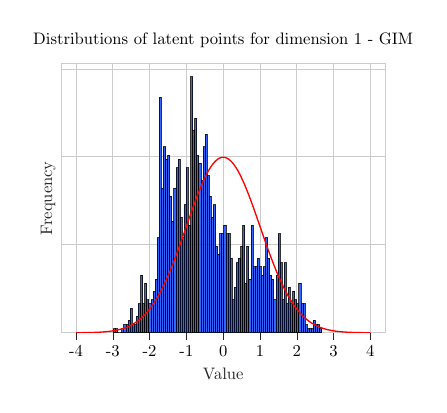
\begin{tikzpicture}[scale=0.6]

\definecolor{blue262255}{RGB}{2,62,255}
\definecolor{darkslategray38}{RGB}{38,38,38}
\definecolor{lightgray204}{RGB}{204,204,204}

\begin{axis}[
	axis line style={lightgray204},
	tick align=outside,
	title={Distributions of latent points for dimension 1 - GIM},
	x grid style={lightgray204},
	xlabel=\textcolor{darkslategray38}{Value},
	xmajorgrids,
	xtick={-5, -4, -3, -2, -1, 0, 1, 2, 3, 4},
	xticklabels={-5, -4, -3, -2, -1, 0, 1, 2, 3, 4},
	xmin=-4.4, xmax=4.4,
 	xtick pos=bottom, % add this line to remove top x-ticks
xtick style={color=darkslategray38},
y grid style={lightgray204},
ylabel=\textcolor{darkslategray38}{Frequency},
ymajorgrids,
ymajorticks=false,
ymin=0, ymax=0.611458894700324,
ytick style={color=darkslategray38}
]
\draw[draw=black,fill=blue262255,opacity=0.8,line width=0.48pt] (axis cs:-2.9815046787262,0) rectangle (axis cs:-2.92490363121033,0.00939261964065994);
\draw[draw=black,fill=blue262255,opacity=0.8,line width=0.48pt] (axis cs:-2.92490386962891,0) rectangle (axis cs:-2.86830258369446,0.00939258007662899);
\draw[draw=black,fill=blue262255,opacity=0.8,line width=0.48pt] (axis cs:-2.86830234527588,0) rectangle (axis cs:-2.81170129776001,0);
\draw[draw=black,fill=blue262255,opacity=0.8,line width=0.48pt] (axis cs:-2.81170129776001,0) rectangle (axis cs:-2.75510025024414,0);
\draw[draw=black,fill=blue262255,opacity=0.8,line width=0.48pt] (axis cs:-2.75510025024414,0) rectangle (axis cs:-2.69849896430969,0.00939258007662899);
\draw[draw=black,fill=blue262255,opacity=0.8,line width=0.48pt] (axis cs:-2.69849896430969,0) rectangle (axis cs:-2.64189791679382,0.0187852392813199);
\draw[draw=black,fill=blue262255,opacity=0.8,line width=0.48pt] (axis cs:-2.64189791679382,0) rectangle (axis cs:-2.58529686927795,0.0187852392813199);
\draw[draw=black,fill=blue262255,opacity=0.8,line width=0.48pt] (axis cs:-2.58529686927795,0) rectangle (axis cs:-2.52869582176208,0.0281778589219798);
\draw[draw=black,fill=blue262255,opacity=0.8,line width=0.48pt] (axis cs:-2.52869606018066,0) rectangle (axis cs:-2.47209477424622,0.0563554804597739);
\draw[draw=black,fill=blue262255,opacity=0.8,line width=0.48pt] (axis cs:-2.47209453582764,0) rectangle (axis cs:-2.41549348831177,0.0187852392813199);
\draw[draw=black,fill=blue262255,opacity=0.8,line width=0.48pt] (axis cs:-2.41549348831177,0) rectangle (axis cs:-2.3588924407959,0.0187852392813199);
\draw[draw=black,fill=blue262255,opacity=0.8,line width=0.48pt] (axis cs:-2.3588924407959,0) rectangle (axis cs:-2.30229115486145,0.0375703203065159);
\draw[draw=black,fill=blue262255,opacity=0.8,line width=0.48pt] (axis cs:-2.30229115486145,0) rectangle (axis cs:-2.24569010734558,0.0657483374846196);
\draw[draw=black,fill=blue262255,opacity=0.8,line width=0.48pt] (axis cs:-2.24569010734558,0) rectangle (axis cs:-2.18908905982971,0.131496674969239);
\draw[draw=black,fill=blue262255,opacity=0.8,line width=0.48pt] (axis cs:-2.18908929824829,0) rectangle (axis cs:-2.13248801231384,0.0657480605364029);
\draw[draw=black,fill=blue262255,opacity=0.8,line width=0.48pt] (axis cs:-2.13248777389526,0) rectangle (axis cs:-2.07588672637939,0.112711435687919);
\draw[draw=black,fill=blue262255,opacity=0.8,line width=0.48pt] (axis cs:-2.07588672637939,0) rectangle (axis cs:-2.01928567886353,0.0751409571252795);
\draw[draw=black,fill=blue262255,opacity=0.8,line width=0.48pt] (axis cs:-2.01928567886353,0) rectangle (axis cs:-1.96268463134766,0.0657481990102196);
\draw[draw=black,fill=blue262255,opacity=0.8,line width=0.48pt] (axis cs:-1.96268439292908,0) rectangle (axis cs:-1.90608334541321,0.0751407988688224);
\draw[draw=black,fill=blue262255,opacity=0.8,line width=0.48pt] (axis cs:-1.90608334541321,0) rectangle (axis cs:-1.84948229789734,0.0939261964065994);
\draw[draw=black,fill=blue262255,opacity=0.8,line width=0.48pt] (axis cs:-1.84948229789734,0) rectangle (axis cs:-1.79288125038147,0.122103798161836);
\draw[draw=black,fill=blue262255,opacity=0.8,line width=0.48pt] (axis cs:-1.79288101196289,0) rectangle (axis cs:-1.73627996444702,0.216029796747864);
\draw[draw=black,fill=blue262255,opacity=0.8,line width=0.48pt] (axis cs:-1.73627996444702,0) rectangle (axis cs:-1.67967891693115,0.535379319517617);
\draw[draw=black,fill=blue262255,opacity=0.8,line width=0.48pt] (axis cs:-1.67967891693115,0) rectangle (axis cs:-1.62307786941528,0.328740995051098);
\draw[draw=black,fill=blue262255,opacity=0.8,line width=0.48pt] (axis cs:-1.6230776309967,0) rectangle (axis cs:-1.56647658348083,0.422666993637126);
\draw[draw=black,fill=blue262255,opacity=0.8,line width=0.48pt] (axis cs:-1.56647658348083,0) rectangle (axis cs:-1.50987553596497,0.394490024907717);
\draw[draw=black,fill=blue262255,opacity=0.8,line width=0.48pt] (axis cs:-1.50987553596497,0) rectangle (axis cs:-1.4532744884491,0.40388179391992);
\draw[draw=black,fill=blue262255,opacity=0.8,line width=0.48pt] (axis cs:-1.45327436923981,0) rectangle (axis cs:-1.39667332172394,0.309956448141778);
\draw[draw=black,fill=blue262255,opacity=0.8,line width=0.48pt] (axis cs:-1.39667320251465,0) rectangle (axis cs:-1.34007215499878,0.253600196182276);
\draw[draw=black,fill=blue262255,opacity=0.8,line width=0.48pt] (axis cs:-1.34007215499878,0) rectangle (axis cs:-1.28347110748291,0.328740995051098);
\draw[draw=black,fill=blue262255,opacity=0.8,line width=0.48pt] (axis cs:-1.28347098827362,0) rectangle (axis cs:-1.22686994075775,0.375704785626398);
\draw[draw=black,fill=blue262255,opacity=0.8,line width=0.48pt] (axis cs:-1.22686982154846,0) rectangle (axis cs:-1.17026877403259,0.394489194061318);
\draw[draw=black,fill=blue262255,opacity=0.8,line width=0.48pt] (axis cs:-1.17026877403259,0) rectangle (axis cs:-1.11366772651672,0.262993349938478);
\draw[draw=black,fill=blue262255,opacity=0.8,line width=0.48pt] (axis cs:-1.11366772651672,0) rectangle (axis cs:-1.05706667900085,0.216029796747864);
\draw[draw=black,fill=blue262255,opacity=0.8,line width=0.48pt] (axis cs:-1.05706644058228,0) rectangle (axis cs:-1.00046539306641,0.291170595616687);
\draw[draw=black,fill=blue262255,opacity=0.8,line width=0.48pt] (axis cs:-1.00046539306641,0) rectangle (axis cs:-0.943864345550537,0.375704389984838);
\draw[draw=black,fill=blue262255,opacity=0.8,line width=0.48pt] (axis cs:-0.943864226341248,0) rectangle (axis cs:-0.887263178825378,0.244207853490145);
\draw[draw=black,fill=blue262255,opacity=0.8,line width=0.48pt] (axis cs:-0.887263178825378,0) rectangle (axis cs:-0.830662131309509,0.582341804476499);
\draw[draw=black,fill=blue262255,opacity=0.8,line width=0.48pt] (axis cs:-0.83066201210022,0) rectangle (axis cs:-0.774060964584351,0.460237877731427);
\draw[draw=black,fill=blue262255,opacity=0.8,line width=0.48pt] (axis cs:-0.774060904979706,0) rectangle (axis cs:-0.717459857463837,0.488415192647346);
\draw[draw=black,fill=blue262255,opacity=0.8,line width=0.48pt] (axis cs:-0.717459797859192,0) rectangle (axis cs:-0.660858750343323,0.403882219233701);
\draw[draw=black,fill=blue262255,opacity=0.8,line width=0.48pt] (axis cs:-0.660858631134033,0) rectangle (axis cs:-0.604257583618164,0.385096999734459);
\draw[draw=black,fill=blue262255,opacity=0.8,line width=0.48pt] (axis cs:-0.604257583618164,0) rectangle (axis cs:-0.547656536102295,0.347526560735975);
\draw[draw=black,fill=blue262255,opacity=0.8,line width=0.48pt] (axis cs:-0.547656416893005,0) rectangle (axis cs:-0.491055369377136,0.422667216184917);
\draw[draw=black,fill=blue262255,opacity=0.8,line width=0.48pt] (axis cs:-0.491055309772491,0) rectangle (axis cs:-0.434454262256622,0.450845030597245);
\draw[draw=black,fill=blue262255,opacity=0.8,line width=0.48pt] (axis cs:-0.434454172849655,0) rectangle (axis cs:-0.377853125333786,0.356919170485596);
\draw[draw=black,fill=blue262255,opacity=0.8,line width=0.48pt] (axis cs:-0.377853035926819,0) rectangle (axis cs:-0.32125198841095,0.309955958535606);
\draw[draw=black,fill=blue262255,opacity=0.8,line width=0.48pt] (axis cs:-0.321251928806305,0) rectangle (axis cs:-0.264650881290436,0.262993072989387);
\draw[draw=black,fill=blue262255,opacity=0.8,line width=0.48pt] (axis cs:-0.264650821685791,0) rectangle (axis cs:-0.208049774169922,0.291170825582798);
\draw[draw=black,fill=blue262255,opacity=0.8,line width=0.48pt] (axis cs:-0.208049684762955,0) rectangle (axis cs:-0.151448637247086,0.197244752814154);
\draw[draw=black,fill=blue262255,opacity=0.8,line width=0.48pt] (axis cs:-0.151448577642441,0) rectangle (axis cs:-0.0948475301265717,0.178459538260425);
\draw[draw=black,fill=blue262255,opacity=0.8,line width=0.48pt] (axis cs:-0.0948474481701851,0) rectangle (axis cs:-0.0382464006543159,0.225422574644747);
\draw[draw=black,fill=blue262255,opacity=0.8,line width=0.48pt] (axis cs:-0.03824632614851,0) rectangle (axis cs:0.0183547213673592,0.225422574644747);
\draw[draw=black,fill=blue262255,opacity=0.8,line width=0.48pt] (axis cs:0.0183547958731651,0) rectangle (axis cs:0.0749558433890343,0.244207789198476);
\draw[draw=black,fill=blue262255,opacity=0.8,line width=0.48pt] (axis cs:0.0749559178948402,0) rectangle (axis cs:0.131556957960129,0.225422574644747);
\draw[draw=black,fill=blue262255,opacity=0.8,line width=0.48pt] (axis cs:0.131557047367096,0) rectangle (axis cs:0.188158094882965,0.225422574644747);
\draw[draw=black,fill=blue262255,opacity=0.8,line width=0.48pt] (axis cs:0.18815815448761,0) rectangle (axis cs:0.244759202003479,0.16906693098356);
\draw[draw=black,fill=blue262255,opacity=0.8,line width=0.48pt] (axis cs:0.244759291410446,0) rectangle (axis cs:0.301360338926315,0.0751408582149157);
\draw[draw=black,fill=blue262255,opacity=0.8,line width=0.48pt] (axis cs:0.30136039853096,0) rectangle (axis cs:0.357961446046829,0.10331870724583);
\draw[draw=black,fill=blue262255,opacity=0.8,line width=0.48pt] (axis cs:0.357961535453796,0) rectangle (axis cs:0.414562582969666,0.159674281669858);
\draw[draw=black,fill=blue262255,opacity=0.8,line width=0.48pt] (axis cs:0.41456264257431,0) rectangle (axis cs:0.471163690090179,0.169066975493177);
\draw[draw=black,fill=blue262255,opacity=0.8,line width=0.48pt] (axis cs:0.471163749694824,0) rectangle (axis cs:0.527764797210693,0.197244700886295);
\draw[draw=black,fill=blue262255,opacity=0.8,line width=0.48pt] (axis cs:0.527764916419983,0) rectangle (axis cs:0.584365963935852,0.244207853490145);
\draw[draw=black,fill=blue262255,opacity=0.8,line width=0.48pt] (axis cs:0.584365963935852,0) rectangle (axis cs:0.640967011451721,0.112711316995451);
\draw[draw=black,fill=blue262255,opacity=0.8,line width=0.48pt] (axis cs:0.640967130661011,0) rectangle (axis cs:0.69756817817688,0.197244597030659);
\draw[draw=black,fill=blue262255,opacity=0.8,line width=0.48pt] (axis cs:0.697568297386169,0) rectangle (axis cs:0.754169344902039,0.122103926745072);
\draw[draw=black,fill=blue262255,opacity=0.8,line width=0.48pt] (axis cs:0.754169344902039,0) rectangle (axis cs:0.810770392417908,0.244207853490145);
\draw[draw=black,fill=blue262255,opacity=0.8,line width=0.48pt] (axis cs:0.810770511627197,0) rectangle (axis cs:0.867371559143066,0.150281755993935);
\draw[draw=black,fill=blue262255,opacity=0.8,line width=0.48pt] (axis cs:0.867371618747711,0) rectangle (axis cs:0.92397266626358,0.150281597737645);
\draw[draw=black,fill=blue262255,opacity=0.8,line width=0.48pt] (axis cs:0.923972725868225,0) rectangle (axis cs:0.980573773384094,0.169066975493177);
\draw[draw=black,fill=blue262255,opacity=0.8,line width=0.48pt] (axis cs:0.980573892593384,0) rectangle (axis cs:1.03717494010925,0.150281755993935);
\draw[draw=black,fill=blue262255,opacity=0.8,line width=0.48pt] (axis cs:1.03717494010925,0) rectangle (axis cs:1.09377598762512,0.131496398020439);
\draw[draw=black,fill=blue262255,opacity=0.8,line width=0.48pt] (axis cs:1.09377610683441,0) rectangle (axis cs:1.15037715435028,0.150281914250559);
\draw[draw=black,fill=blue262255,opacity=0.8,line width=0.48pt] (axis cs:1.15037727355957,0) rectangle (axis cs:1.20697832107544,0.216029796747864);
\draw[draw=black,fill=blue262255,opacity=0.8,line width=0.48pt] (axis cs:1.20697832107544,0) rectangle (axis cs:1.26357936859131,0.169067153531879);
\draw[draw=black,fill=blue262255,opacity=0.8,line width=0.48pt] (axis cs:1.26357936859131,0) rectangle (axis cs:1.32018041610718,0.131496398020439);
\draw[draw=black,fill=blue262255,opacity=0.8,line width=0.48pt] (axis cs:1.32018065452576,0) rectangle (axis cs:1.37678170204163,0.122103798161836);
\draw[draw=black,fill=blue262255,opacity=0.8,line width=0.48pt] (axis cs:1.37678170204163,0) rectangle (axis cs:1.4333827495575,0.0751409571252795);
\draw[draw=black,fill=blue262255,opacity=0.8,line width=0.48pt] (axis cs:1.4333827495575,0) rectangle (axis cs:1.48998379707336,0.131496398020439);
\draw[draw=black,fill=blue262255,opacity=0.8,line width=0.48pt] (axis cs:1.48998403549194,0) rectangle (axis cs:1.54658508300781,0.225422396606467);
\draw[draw=black,fill=blue262255,opacity=0.8,line width=0.48pt] (axis cs:1.54658508300781,0) rectangle (axis cs:1.60318613052368,0.159674533891219);
\draw[draw=black,fill=blue262255,opacity=0.8,line width=0.48pt] (axis cs:1.60318613052368,0) rectangle (axis cs:1.65978717803955,0.0751407988688224);
\draw[draw=black,fill=blue262255,opacity=0.8,line width=0.48pt] (axis cs:1.65978729724884,0) rectangle (axis cs:1.71638834476471,0.159674533891219);
\draw[draw=black,fill=blue262255,opacity=0.8,line width=0.48pt] (axis cs:1.716388463974,0) rectangle (axis cs:1.77298951148987,0.0657481990102196);
\draw[draw=black,fill=blue262255,opacity=0.8,line width=0.48pt] (axis cs:1.77298951148987,0) rectangle (axis cs:1.82959055900574,0.103318598444631);
\draw[draw=black,fill=blue262255,opacity=0.8,line width=0.48pt] (axis cs:1.82959067821503,0) rectangle (axis cs:1.8861917257309,0.0657483374846196);
\draw[draw=black,fill=blue262255,opacity=0.8,line width=0.48pt] (axis cs:1.88619184494019,0) rectangle (axis cs:1.94279289245605,0.093925998586028);
\draw[draw=black,fill=blue262255,opacity=0.8,line width=0.48pt] (axis cs:1.94279289245605,0) rectangle (axis cs:1.99939393997192,0.0751407988688224);
\draw[draw=black,fill=blue262255,opacity=0.8,line width=0.48pt] (axis cs:1.9993941783905,0) rectangle (axis cs:2.05599522590637,0.0657481990102196);
\draw[draw=black,fill=blue262255,opacity=0.8,line width=0.48pt] (axis cs:2.05599522590637,0) rectangle (axis cs:2.11259627342224,0.112711435687919);
\draw[draw=black,fill=blue262255,opacity=0.8,line width=0.48pt] (axis cs:2.11259627342224,0) rectangle (axis cs:2.16919732093811,0.0657483374846196);
\draw[draw=black,fill=blue262255,opacity=0.8,line width=0.48pt] (axis cs:2.16919708251953,0) rectangle (axis cs:2.22579836845398,0.0657480605364029);
\draw[draw=black,fill=blue262255,opacity=0.8,line width=0.48pt] (axis cs:2.22579860687256,0) rectangle (axis cs:2.28239965438843,0.0187852392813199);
\draw[draw=black,fill=blue262255,opacity=0.8,line width=0.48pt] (axis cs:2.28239965438843,0) rectangle (axis cs:2.3390007019043,0.00939261964065994);
\draw[draw=black,fill=blue262255,opacity=0.8,line width=0.48pt] (axis cs:2.3390007019043,0) rectangle (axis cs:2.39560174942017,0.00939261964065994);
\draw[draw=black,fill=blue262255,opacity=0.8,line width=0.48pt] (axis cs:2.39560174942017,0) rectangle (axis cs:2.45220303535461,0.00939258007662899);
\draw[draw=black,fill=blue262255,opacity=0.8,line width=0.48pt] (axis cs:2.45220303535461,0) rectangle (axis cs:2.50880408287048,0.0281778589219798);
\draw[draw=black,fill=blue262255,opacity=0.8,line width=0.48pt] (axis cs:2.50880408287048,0) rectangle (axis cs:2.56540513038635,0.0187852392813199);
\draw[draw=black,fill=blue262255,opacity=0.8,line width=0.48pt] (axis cs:2.56540489196777,0) rectangle (axis cs:2.62200617790222,0.018785160153258);
\draw[draw=black,fill=blue262255,opacity=0.8,line width=0.48pt] (axis cs:2.6220064163208,0) rectangle (axis cs:2.67860746383667,0.00939261964065994);
\addplot [thick, red]
table {%
-4 0.000133830225764885
-3.99199199199199 0.000138182046410498
-3.98398398398398 0.000142666228042307
-3.97597597597598 0.000147286481503254
-3.96796796796797 0.000152046611333821
-3.95995995995996 0.000156950517814782
-3.95195195195195 0.00016200219904485
-3.94394394394394 0.00016720575305353
-3.93593593593594 0.000172565379949496
-3.92792792792793 0.00017808538410479
-3.91991991991992 0.000183770176375138
-3.91191191191191 0.000189624276356684
-3.9039039039039 0.000195652314679408
-3.8958958958959 0.000201859035337517
-3.88788788788789 0.000208249298057069
-3.87987987987988 0.000214828080701088
-3.87187187187187 0.000221600481712426
-3.86386386386386 0.0002285717225946
-3.85585585585586 0.000235747150430845
-3.84784784784785 0.000243132240441603
-3.83983983983984 0.000250732598580649
-3.83183183183183 0.000258553964170059
-3.82382382382382 0.000266602212574213
-3.81581581581582 0.000274883357912987
-3.80780780780781 0.000283403555814325
-3.7997997997998 0.000292169106206322
-3.79179179179179 0.000301186456148957
-3.78378378378378 0.0003104622027056
-3.77577577577578 0.000320003095854415
-3.76776776776777 0.000329816041439723
-3.75975975975976 0.000339908104163431
-3.75175175175175 0.00035028651061658
-3.74374374374374 0.000360958652351047
-3.73573573573574 0.000371932088991451
-3.72772772772773 0.000383214551387261
-3.71971971971972 0.000394813944805093
-3.71171171171171 0.000406738352161197
-3.7037037037037 0.000418996037294058
-3.6956956956957 0.00043159544827708
-3.68768768768769 0.00044454522077123
-3.67967967967968 0.000457854181417586
-3.67167167167167 0.000471531351269624
-3.66366366366366 0.000485585949265103
-3.65565565565566 0.000500027395737409
-3.64764764764765 0.000514865315966112
-3.63963963963964 0.000530109543766577
-3.63163163163163 0.000545770125118336
-3.62362362362362 0.000561857321831991
-3.61561561561562 0.00057838161525435
-3.60760760760761 0.000595353710011453
-3.5995995995996 0.000612784537789192
-3.59159159159159 0.000630685261151105
-3.58358358358358 0.000649067277392973
-3.57557557557558 0.000667942222433796
-3.56756756756757 0.000687321974742665
-3.55955955955956 0.000707218659301081
-3.55155155155155 0.000727644651600166
-3.54354354354354 0.000748612581672245
-3.53553553553554 0.000770135338156225
-3.52752752752753 0.000792226072396121
-3.51951951951952 0.00081489820257214
-3.51151151151151 0.000838165417863603
-3.5035035035035 0.000862041682643007
-3.4954954954955 0.000886541240700502
-3.48748748748749 0.00091167861949796
-3.47947947947948 0.000937468634451866
-3.47147147147147 0.000963926393244149
-3.46346346346346 0.000991067300160059
-3.45545545545546 0.0010189070604522
-3.44744744744745 0.00104746168472971
-3.43943943943944 0.0010767474933716
-3.43143143143143 0.00110678112096323
-3.42342342342342 0.00113757952075483
-3.41541541541542 0.00116915996914087
-3.40740740740741 0.00120154007015926
-3.3993993993994 0.00123473776000907
-3.39139139139139 0.00126877131158549
-3.38338338338338 0.00130365933903088
-3.37537537537538 0.00133942080230046
-3.36736736736737 0.00137607501174126
-3.35935935935936 0.001413641632683
-3.35135135135135 0.00145214069003938
-3.34334334334334 0.0014915925729182
-3.33533533533534 0.00153201803923895
-3.32732732732733 0.00157343822035606
-3.31931931931932 0.00161587462568624
-3.31131131131131 0.00165934914733831
-3.3033033033033 0.00170388406474362
-3.2952952952953 0.00174950204928538
-3.28728728728729 0.00179622616892505
-3.27927927927928 0.00184407989282385
-3.27127127127127 0.00189308709595757
-3.26326326326326 0.00194327206372255
-3.25525525525526 0.00199465949653091
-3.24724724724725 0.00204727451439301
-3.23923923923924 0.00210114266148476
-3.23123123123123 0.00215628991069791
-3.22322322322322 0.00221274266817093
-3.21521521521522 0.00227052777779815
-3.20720720720721 0.00232967252571501
-3.1991991991992 0.00239020464475689
-3.19119119119119 0.00245215231888918
-3.18318318318318 0.00251554418760605
-3.17517517517518 0.00258040935029545
-3.16716716716717 0.00264677737056774
-3.15915915915916 0.00271467828054534
-3.15115115115115 0.00278414258511061
-3.14314314314314 0.00285520126610952
-3.13513513513514 0.00292788578650791
-3.12712712712713 0.00300222809449793
-3.11911911911912 0.00307826062755151
-3.11111111111111 0.00315601631641804
-3.1031031031031 0.00323552858906328
-3.0950950950951 0.00331683137454643
-3.08708708708709 0.00339995910683238
-3.07907907907908 0.00348494672853595
-3.07107107107107 0.00357182969459489
-3.06306306306306 0.00366064397586864
-3.05505505505506 0.00375142606265932
-3.04704704704705 0.00384421296815189
-3.03903903903904 0.00393904223176991
-3.03103103103103 0.00403595192244368
-3.02302302302302 0.0041349806417872
-3.01501501501502 0.00423616752718052
-3.00700700700701 0.00433955225475399
-2.998998998999 0.00444517504227068
-2.99099099099099 0.00455307665190355
-2.98298298298298 0.00466329839290368
-2.97497497497497 0.00477588212415564
-2.96696696696697 0.00489087025661667
-2.95895895895896 0.00500830575563558
-2.95095095095095 0.00512823214314763
-2.94294294294294 0.00525069349974172
-2.93493493493493 0.00537573446659573
-2.92692692692693 0.00550340024727644
-2.91891891891892 0.00563373660939975
-2.91091091091091 0.0057667898861475
-2.9029029029029 0.00590260697763674
-2.89489489489489 0.00604123535213746
-2.88688688688689 0.00618272304713484
-2.87887887887888 0.00632711867023164
-2.87087087087087 0.00647447139988703
-2.86286286286286 0.00662483098598741
-2.85485485485485 0.0067782477502453
-2.84684684684685 0.0069347725864219
-2.83883883883884 0.00709445696036946
-2.83083083083083 0.00725735290988893
-2.82282282282282 0.00742351304439893
-2.81481481481481 0.00759299054441176
-2.80680680680681 0.0077658391608121
-2.7987987987988 0.00794211321393437
-2.79079079079079 0.00812186759243432
-2.78278278278278 0.00830515775195071
-2.77477477477477 0.00849203971355293
-2.76676676676677 0.00868257006197001
-2.75875875875876 0.00887680594359712
-2.75075075075075 0.00907480506427511
-2.74274274274274 0.00927662568683898
-2.73473473473473 0.00948232662843099
-2.72672672672673 0.00969196725757422
-2.71871871871872 0.00990560749100246
-2.71071071071071 0.0101233077902421
-2.7027027027027 0.0103451291579421
-2.69469469469469 0.0105711331339476
-2.68668668668669 0.0108013817911136
-2.67867867867868 0.011035937730854
-2.67067067067067 0.0112748640784219
-2.66266266266266 0.0115182244779185
-2.65465465465465 0.0117660830870247
-2.64664664664665 0.0120185045714526
-2.63863863863864 0.0122755540991133
-2.63063063063063 0.0125372973339956
-2.62262262262262 0.0128038004297541
-2.61461461461461 0.0130751300230007
-2.60660660660661 0.0133513532262973
-2.5985985985986 0.0136325376208454
-2.59059059059059 0.0139187512488692
-2.58258258258258 0.014210062605689
-2.57457457457457 0.0145065406314803
-2.56656656656657 0.0148082547027168
-2.55855855855856 0.0151152746232934
-2.55055055055055 0.0154276706153247
-2.54254254254254 0.0157455133096184
-2.53453453453453 0.0160688737358178
-2.52652652652653 0.016397823312213
-2.51851851851852 0.0167324338352151
-2.51051051051051 0.0170727774684938
-2.5025025025025 0.0174189267317727
-2.49449449449449 0.0177709544892815
-2.48648648648649 0.0181289339378627
-2.47847847847848 0.0184929385947284
-2.47047047047047 0.0188630422848682
-2.46246246246246 0.0192393191281025
-2.45445445445445 0.0196218435257817
-2.44644644644645 0.0200106901471285
-2.43843843843844 0.020405933915221
-2.43043043043043 0.0208076499926159
-2.42242242242242 0.0212159137666093
-2.41441441441441 0.0216308008341344
-2.40640640640641 0.0220523869862944
-2.3983983983984 0.0224807481925294
-2.39039039039039 0.022915960584417
-2.38238238238238 0.0233581004391047
-2.37437437437437 0.023807244162374
-2.36636636636637 0.0242634682713357
-2.35835835835836 0.0247268493767558
-2.35035035035035 0.0251974641650118
-2.34234234234234 0.0256753893796796
-2.33433433433433 0.0261607018027501
-2.32632632632633 0.0266534782354775
-2.31831831831832 0.0271537954788581
-2.31031031031031 0.0276617303137407
-2.3023023023023 0.0281773594805703
-2.29429429429429 0.0287007596587648
-2.28628628628629 0.0292320074457259
-2.27827827827828 0.029771179335487
-2.27027027027027 0.0303183516969979
-2.26226226226226 0.0308736007520491
-2.25425425425425 0.0314370025528369
-2.24624624624625 0.0320086329591723
-2.23823823823824 0.0325885676153351
-2.23023023023023 0.0331768819265761
-2.22222222222222 0.0337736510352706
-2.21421421421421 0.0343789497967251
-2.20620620620621 0.0349928527546413
-2.1981981981982 0.0356154341162401
-2.19019019019019 0.0362467677270497
-2.18218218218218 0.0368869270453615
-2.17417417417417 0.0375359851163567
-2.16616616616617 0.03819401454591
-2.15815815815816 0.0388610874740724
-2.15015015015015 0.03953727554824
-2.14214214214214 0.0402226498960119
-2.13413413413413 0.0409172810977437
-2.12612612612613 0.0416212391588003
-2.11811811811812 0.0423345934815158
-2.11011011011011 0.0430574128368641
-2.1021021021021 0.043789765335848
-2.09409409409409 0.0445317184006117
-2.08608608608609 0.0452833387352837
-2.07807807807808 0.0460446922965577
-2.07007007007007 0.0468158442640166
-2.06206206206206 0.0475968590102091
-2.05405405405405 0.0483878000704834
-2.04604604604605 0.0491887301125894
-2.03803803803804 0.0499997109060533
-2.03003003003003 0.0508208032913361
-2.02202202202202 0.0516520671487823
-2.01401401401401 0.0524935613673682
-2.00600600600601 0.053345343813258
-1.997997997998 0.0542074712981785
-1.98998998998999 0.0550799995476186
-1.98198198198198 0.0559629831688668
-1.97397397397397 0.0568564756188931
-1.96596596596597 0.0577605291720876
-1.95795795795796 0.0586751948878651
-1.94994994994995 0.0596005225781457
-1.94194194194194 0.0605365607747232
-1.93393393393393 0.0614833566965309
-1.92592592592593 0.062440956216817
-1.91791791791792 0.06340940383024
-1.90990990990991 0.0643887426198963
-1.9019019019019 0.0653790142242912
-1.89389389389389 0.0663802588042656
-1.88588588588589 0.0673925150098903
-1.87787787787788 0.0684158199473405
-1.86986986986987 0.0694502091457625
-1.86186186186186 0.0704957165241465
-1.85385385385385 0.0715523743582165
-1.84584584584585 0.0726202132473521
-1.83783783783784 0.0736992620815557
-1.82982982982983 0.0747895480084762
-1.82182182182182 0.0758910964005057
-1.81381381381381 0.0770039308219614
-1.80580580580581 0.0781280729963669
-1.7977977977978 0.0792635427738473
-1.78978978978979 0.0804103580986525
-1.78178178178178 0.0815685349768227
-1.77377377377377 0.0827380874440109
-1.76576576576577 0.0839190275334777
-1.75775775775776 0.0851113652442723
-1.74974974974975 0.086315108509615
-1.74174174174174 0.0875302631654975
-1.73373373373373 0.0887568329195139
-1.72572572572573 0.0899948193199405
-1.71771771771772 0.0912442217250772
-1.70970970970971 0.0925050372728685
-1.7017017017017 0.0937772608508177
-1.69369369369369 0.0950608850662112
-1.68568568568569 0.0963559002166691
-1.67767767767768 0.0976622942610365
-1.66966966966967 0.0989800527906321
-1.66166166166166 0.100309159000872
-1.65365365365365 0.10164959366328
-1.64564564564565 0.103001335097907
-1.63763763763764 0.10436435914617
-1.62962962962963 0.105738639144131
-1.62162162162162 0.107124145896225
-1.61361361361361 0.108520847649465
-1.60560560560561 0.10992871006813
-1.5975975975976 0.111347696208955
-1.58958958958959 0.112777766496842
-1.58158158158158 0.114218878701105
-1.57357357357357 0.115670987912262
-1.56556556556557 0.117134046519405
-1.55755755755756 0.11860800418814
-1.54954954954955 0.120092807839133
-1.54154154154154 0.121588401627275
-1.53353353353353 0.123094726921466
-1.52552552552553 0.124611722285057
-1.51751751751752 0.12613932345695
-1.50950950950951 0.127677463333369
-1.5015015015015 0.129226071950339
-1.49349349349349 0.130785076466857
-1.48548548548549 0.132354401148798
-1.47747747747748 0.133933967353555
-1.46946946946947 0.13552369351543
-1.46146146146146 0.137123495131801
-1.45345345345345 0.13873328475006
-1.44544544544545 0.140352971955359
-1.43743743743744 0.141982463359159
-1.42942942942943 0.143621662588612
-1.42142142142142 0.14527047027677
-1.41341341341341 0.146928784053658
-1.40540540540541 0.148596498538208
-1.3973973973974 0.150273505331067
-1.38938938938939 0.151959693008306
-1.38138138138138 0.153654947116025
-1.37337337337337 0.155359150165875
-1.36536536536537 0.157072181631514
-1.35735735735736 0.158793917945997
-1.34934934934935 0.160524232500121
-1.34134134134134 0.16226299564173
-1.33333333333333 0.164010074675994
-1.32532532532533 0.165765333866673
-1.31731731731732 0.167528634438376
-1.30930930930931 0.169299834579821
-1.3013013013013 0.17107878944811
-1.29329329329329 0.172865351174024
-1.28528528528529 0.174659368868355
-1.27727727727728 0.176460688629273
-1.26926926926927 0.178269153550739
-1.26126126126126 0.180084603731981
-1.25325325325325 0.181906876288021
-1.24524524524525 0.183735805361283
-1.23723723723724 0.185571222134271
-1.22922922922923 0.187412954843324
-1.22122122122122 0.18926082879347
-1.21321321321321 0.191114666374361
-1.20520520520521 0.192974287077311
-1.1971971971972 0.194839507513435
-1.18918918918919 0.19671014143289
-1.18118118118118 0.198585999745227
-1.17317317317317 0.200466890540856
-1.16516516516517 0.202352619113618
-1.15715715715716 0.204242987984477
-1.14914914914915 0.206137796926331
-1.14114114114114 0.208036842989938
-1.13313313313313 0.209939920530956
-1.12512512512513 0.21184682123811
-1.11711711711712 0.21375733416247
-1.10910910910911 0.215671245747847
-1.1011011011011 0.217588339862305
-1.09309309309309 0.219508397830784
-1.08508508508509 0.221431198468836
-1.07707707707708 0.223356518117463
-1.06906906906907 0.225284130679063
-1.06106106106106 0.22721380765447
-1.05305305305305 0.229145318181096
-1.04504504504505 0.231078429072154
-1.03703703703704 0.233012904856966
-1.02902902902903 0.234948507822352
-1.02102102102102 0.236884998055083
-1.01301301301301 0.238822133485401
-1.00500500500501 0.24075966993159
-0.996996996996997 0.242697361145593
-0.988988988988989 0.244634958859672
-0.980980980980981 0.246572212834085
-0.972972972972973 0.248508870905785
-0.964964964964965 0.250444679038131
-0.956956956956957 0.252379381371581
-0.948948948948949 0.254312720275385
-0.940940940940941 0.256244436400228
-0.932932932932933 0.258174268731856
-0.924924924924925 0.260101954645624
-0.916916916916917 0.262027229961987
-0.908908908908909 0.263949829002911
-0.900900900900901 0.265869484649172
-0.892892892892893 0.267785928398552
-0.884884884884885 0.269698890424904
-0.876876876876877 0.271608099638066
-0.868868868868869 0.273513283744617
-0.860860860860861 0.275414169309444
-0.852852852852853 0.277310481818125
-0.844844844844845 0.279201945740075
-0.836836836836837 0.281088284592474
-0.828828828828829 0.28296922100493
-0.820820820820821 0.284844476784867
-0.812812812812813 0.286713772983616
-0.804804804804805 0.288576829963198
-0.796796796796797 0.290433367463758
-0.788788788788789 0.292283104671645
-0.780780780780781 0.294125760288111
-0.772772772772773 0.295961052598604
-0.764764764764765 0.29778869954263
-0.756756756756757 0.299608418784177
-0.748748748748749 0.301419927782648
-0.740740740740741 0.303222943864308
-0.732732732732733 0.305017184294205
-0.724724724724725 0.306802366348536
-0.716716716716717 0.308578207387456
-0.708708708708709 0.310344424928268
-0.700700700700701 0.312100736719007
-0.692692692692693 0.313846860812361
-0.684684684684685 0.31558251563992
-0.676676676676677 0.317307420086723
-0.668668668668669 0.319021293566066
-0.660660660660661 0.320723856094559
-0.652652652652653 0.322414828367396
-0.644644644644645 0.324093931833804
-0.636636636636636 0.325760888772662
-0.628628628628629 0.327415422368237
-0.620620620620621 0.329057256786028
-0.612612612612613 0.330686117248681
-0.604604604604605 0.33230173011195
-0.596596596596596 0.333903822940662
-0.588588588588589 0.335492124584683
-0.580580580580581 0.337066365254824
-0.572572572572573 0.338626276598684
-0.564564564564565 0.340171591776383
-0.556556556556556 0.341702045536168
-0.548548548548549 0.343217374289848
-0.54054054054054 0.344717316188045
-0.532532532532533 0.346201611195215
-0.524524524524525 0.347670001164422
-0.516516516516516 0.349122229911825
-0.508508508508509 0.350558043290856
-0.5005005005005 0.351977189266054
-0.492492492492492 0.353379417986526
-0.484484484484485 0.354764481859011
-0.476476476476476 0.356132135620502
-0.468468468468469 0.357482136410418
-0.46046046046046 0.358814243842273
-0.452452452452452 0.360128220074839
-0.444444444444445 0.361423829882744
-0.436436436436436 0.362700840726495
-0.428428428428429 0.363959022821904
-0.42042042042042 0.365198149208855
-0.412412412412412 0.366417995819425
-0.404404404404405 0.3676183415453
-0.396396396396396 0.368798968304465
-0.388388388388389 0.369959661107154
-0.38038038038038 0.37110020812101
-0.372372372372372 0.372220400735444
-0.364364364364365 0.373320033625156
-0.356356356356356 0.374398904812801
-0.348348348348348 0.375456815730761
-0.34034034034034 0.376493571282005
-0.332332332332332 0.377508979900006
-0.324324324324325 0.378502853607702
-0.316316316316316 0.379475008075448
-0.308308308308308 0.380425262677969
-0.3003003003003 0.38135344055026
-0.292292292292292 0.382259368642425
-0.284284284284285 0.38314287777343
-0.276276276276276 0.384003802683735
-0.268268268268268 0.3848419820868
-0.26026026026026 0.385657258719425
-0.252252252252252 0.386449479390916
-0.244244244244244 0.387218495031049
-0.236236236236236 0.387964160736805
-0.228228228228228 0.38868633581787
-0.22022022022022 0.389384883840873
-0.212212212212212 0.390059672672329
-0.204204204204204 0.390710574520297
-0.196196196196196 0.391337465974705
-0.188188188188188 0.39194022804635
-0.18018018018018 0.392518746204527
-0.172172172172172 0.393072910413305
-0.164164164164164 0.393602615166401
-0.156156156156156 0.394107759520658
-0.148148148148148 0.394588247128102
-0.14014014014014 0.395043986266573
-0.132132132132132 0.3954748898689
-0.124124124124124 0.395880875550626
-0.116116116116116 0.396261865636259
-0.108108108108108 0.396617787184037
-0.1001001001001 0.396948572009207
-0.0920920920920922 0.397254156705792
-0.084084084084084 0.397534482666846
-0.0760760760760761 0.39778949610319
-0.0680680680680683 0.39801914806061
-0.06006006006006 0.398223394435522
-0.0520520520520522 0.398402195989086
-0.0440440440440439 0.398555518359772
-0.0360360360360361 0.398683332074364
-0.0280280280280278 0.398785612557403
-0.02002002002002 0.398862340139061
-0.0120120120120122 0.398913500061449
-0.00400400400400391 0.398939082483343
0.00400400400400436 0.398939082483343
0.0120120120120122 0.398913500061449
0.02002002002002 0.398862340139061
0.0280280280280278 0.398785612557403
0.0360360360360357 0.398683332074364
0.0440440440440444 0.398555518359772
0.0520520520520522 0.398402195989086
0.06006006006006 0.398223394435522
0.0680680680680679 0.39801914806061
0.0760760760760757 0.39778949610319
0.0840840840840844 0.397534482666846
0.0920920920920922 0.397254156705792
0.1001001001001 0.396948572009207
0.108108108108108 0.396617787184037
0.116116116116116 0.396261865636259
0.124124124124124 0.395880875550626
0.132132132132132 0.3954748898689
0.14014014014014 0.395043986266573
0.148148148148148 0.394588247128102
0.156156156156156 0.394107759520658
0.164164164164164 0.393602615166401
0.172172172172172 0.393072910413305
0.18018018018018 0.392518746204527
0.188188188188188 0.39194022804635
0.196196196196196 0.391337465974705
0.204204204204204 0.390710574520297
0.212212212212212 0.390059672672329
0.22022022022022 0.389384883840873
0.228228228228228 0.388686335817871
0.236236236236236 0.387964160736805
0.244244244244245 0.387218495031049
0.252252252252252 0.386449479390916
0.26026026026026 0.385657258719425
0.268268268268268 0.3848419820868
0.276276276276276 0.384003802683735
0.284284284284285 0.38314287777343
0.292292292292292 0.382259368642425
0.3003003003003 0.38135344055026
0.308308308308308 0.380425262677969
0.316316316316316 0.379475008075448
0.324324324324325 0.378502853607702
0.332332332332332 0.377508979900006
0.34034034034034 0.376493571282005
0.348348348348348 0.375456815730762
0.356356356356356 0.374398904812801
0.364364364364365 0.373320033625156
0.372372372372372 0.372220400735444
0.38038038038038 0.37110020812101
0.388388388388388 0.369959661107154
0.396396396396397 0.368798968304465
0.404404404404405 0.3676183415453
0.412412412412412 0.366417995819425
0.42042042042042 0.365198149208855
0.428428428428428 0.363959022821904
0.436436436436437 0.362700840726495
0.444444444444445 0.361423829882744
0.452452452452452 0.360128220074839
0.46046046046046 0.358814243842273
0.468468468468468 0.357482136410418
0.476476476476477 0.356132135620502
0.484484484484485 0.354764481859011
0.492492492492492 0.353379417986526
0.5005005005005 0.351977189266054
0.508508508508508 0.350558043290856
0.516516516516517 0.349122229911825
0.524524524524525 0.347670001164422
0.532532532532533 0.346201611195215
0.54054054054054 0.344717316188045
0.548548548548548 0.343217374289848
0.556556556556557 0.341702045536168
0.564564564564565 0.340171591776383
0.572572572572573 0.338626276598684
0.58058058058058 0.337066365254824
0.588588588588588 0.335492124584683
0.596596596596597 0.333903822940662
0.604604604604605 0.33230173011195
0.612612612612613 0.330686117248681
0.62062062062062 0.329057256786028
0.628628628628628 0.327415422368237
0.636636636636637 0.325760888772662
0.644644644644645 0.324093931833804
0.652652652652653 0.322414828367396
0.66066066066066 0.32072385609456
0.668668668668668 0.319021293566066
0.676676676676677 0.317307420086723
0.684684684684685 0.31558251563992
0.692692692692693 0.313846860812361
0.7007007007007 0.312100736719007
0.708708708708708 0.310344424928268
0.716716716716717 0.308578207387456
0.724724724724725 0.306802366348536
0.732732732732733 0.305017184294205
0.74074074074074 0.303222943864308
0.748748748748748 0.301419927782648
0.756756756756757 0.299608418784177
0.764764764764765 0.29778869954263
0.772772772772773 0.295961052598604
0.780780780780781 0.294125760288111
0.788788788788788 0.292283104671645
0.796796796796797 0.290433367463758
0.804804804804805 0.288576829963198
0.812812812812813 0.286713772983616
0.820820820820821 0.284844476784867
0.828828828828828 0.282969221004931
0.836836836836837 0.281088284592474
0.844844844844845 0.279201945740075
0.852852852852853 0.277310481818125
0.860860860860861 0.275414169309444
0.868868868868869 0.273513283744617
0.876876876876877 0.271608099638066
0.884884884884885 0.269698890424904
0.892892892892893 0.267785928398552
0.900900900900901 0.265869484649172
0.908908908908909 0.263949829002911
0.916916916916917 0.262027229961987
0.924924924924925 0.260101954645624
0.932932932932933 0.258174268731856
0.940940940940941 0.256244436400228
0.948948948948949 0.254312720275384
0.956956956956957 0.252379381371581
0.964964964964965 0.250444679038131
0.972972972972973 0.248508870905785
0.980980980980981 0.246572212834085
0.988988988988989 0.244634958859672
0.996996996996997 0.242697361145593
1.00500500500501 0.24075966993159
1.01301301301301 0.238822133485401
1.02102102102102 0.236884998055083
1.02902902902903 0.234948507822352
1.03703703703704 0.233012904856966
1.04504504504505 0.231078429072154
1.05305305305305 0.229145318181096
1.06106106106106 0.22721380765447
1.06906906906907 0.225284130679062
1.07707707707708 0.223356518117463
1.08508508508509 0.221431198468836
1.09309309309309 0.219508397830784
1.1011011011011 0.217588339862305
1.10910910910911 0.215671245747847
1.11711711711712 0.21375733416247
1.12512512512513 0.21184682123811
1.13313313313313 0.209939920530956
1.14114114114114 0.208036842989938
1.14914914914915 0.206137796926331
1.15715715715716 0.204242987984477
1.16516516516517 0.202352619113618
1.17317317317317 0.200466890540856
1.18118118118118 0.198585999745228
1.18918918918919 0.19671014143289
1.1971971971972 0.194839507513435
1.20520520520521 0.192974287077311
1.21321321321321 0.191114666374361
1.22122122122122 0.18926082879347
1.22922922922923 0.187412954843324
1.23723723723724 0.185571222134271
1.24524524524525 0.183735805361283
1.25325325325325 0.181906876288021
1.26126126126126 0.180084603731981
1.26926926926927 0.178269153550739
1.27727727727728 0.176460688629273
1.28528528528529 0.174659368868355
1.29329329329329 0.172865351174024
1.3013013013013 0.17107878944811
1.30930930930931 0.169299834579821
1.31731731731732 0.167528634438376
1.32532532532533 0.165765333866673
1.33333333333333 0.164010074675994
1.34134134134134 0.16226299564173
1.34934934934935 0.160524232500121
1.35735735735736 0.158793917945997
1.36536536536537 0.157072181631514
1.37337337337337 0.155359150165875
1.38138138138138 0.153654947116025
1.38938938938939 0.151959693008306
1.3973973973974 0.150273505331067
1.40540540540541 0.148596498538208
1.41341341341341 0.146928784053658
1.42142142142142 0.14527047027677
1.42942942942943 0.143621662588612
1.43743743743744 0.141982463359159
1.44544544544545 0.140352971955359
1.45345345345345 0.13873328475006
1.46146146146146 0.137123495131801
1.46946946946947 0.13552369351543
1.47747747747748 0.133933967353555
1.48548548548549 0.132354401148798
1.49349349349349 0.130785076466857
1.5015015015015 0.129226071950339
1.50950950950951 0.127677463333369
1.51751751751752 0.12613932345695
1.52552552552553 0.124611722285057
1.53353353353353 0.123094726921466
1.54154154154154 0.121588401627275
1.54954954954955 0.120092807839133
1.55755755755756 0.11860800418814
1.56556556556557 0.117134046519405
1.57357357357357 0.115670987912262
1.58158158158158 0.114218878701105
1.58958958958959 0.112777766496842
1.5975975975976 0.111347696208955
1.60560560560561 0.10992871006813
1.61361361361361 0.108520847649465
1.62162162162162 0.107124145896225
1.62962962962963 0.105738639144131
1.63763763763764 0.10436435914617
1.64564564564565 0.103001335097907
1.65365365365365 0.10164959366328
1.66166166166166 0.100309159000872
1.66966966966967 0.0989800527906321
1.67767767767768 0.0976622942610365
1.68568568568569 0.0963559002166692
1.69369369369369 0.0950608850662112
1.7017017017017 0.0937772608508176
1.70970970970971 0.0925050372728685
1.71771771771772 0.0912442217250772
1.72572572572573 0.0899948193199405
1.73373373373373 0.088756832919514
1.74174174174174 0.0875302631654974
1.74974974974975 0.086315108509615
1.75775775775776 0.0851113652442723
1.76576576576577 0.0839190275334778
1.77377377377377 0.082738087444011
1.78178178178178 0.0815685349768226
1.78978978978979 0.0804103580986525
1.7977977977978 0.0792635427738473
1.80580580580581 0.0781280729963669
1.81381381381381 0.0770039308219615
1.82182182182182 0.0758910964005057
1.82982982982983 0.0747895480084762
1.83783783783784 0.0736992620815557
1.84584584584585 0.0726202132473522
1.85385385385385 0.0715523743582165
1.86186186186186 0.0704957165241465
1.86986986986987 0.0694502091457625
1.87787787787788 0.0684158199473405
1.88588588588589 0.0673925150098903
1.89389389389389 0.0663802588042655
1.9019019019019 0.0653790142242912
1.90990990990991 0.0643887426198963
1.91791791791792 0.06340940383024
1.92592592592593 0.0624409562168171
1.93393393393393 0.0614833566965309
1.94194194194194 0.0605365607747232
1.94994994994995 0.0596005225781457
1.95795795795796 0.0586751948878651
1.96596596596597 0.0577605291720876
1.97397397397397 0.056856475618893
1.98198198198198 0.0559629831688668
1.98998998998999 0.0550799995476186
1.997997997998 0.0542074712981785
2.00600600600601 0.0533453438132581
2.01401401401401 0.0524935613673681
2.02202202202202 0.0516520671487823
2.03003003003003 0.0508208032913361
2.03803803803804 0.0499997109060533
2.04604604604605 0.0491887301125894
2.05405405405405 0.0483878000704834
2.06206206206206 0.0475968590102091
2.07007007007007 0.0468158442640166
2.07807807807808 0.0460446922965577
2.08608608608609 0.0452833387352837
2.09409409409409 0.0445317184006117
2.1021021021021 0.043789765335848
2.11011011011011 0.0430574128368641
2.11811811811812 0.0423345934815158
2.12612612612613 0.0416212391588004
2.13413413413413 0.0409172810977437
2.14214214214214 0.0402226498960119
2.15015015015015 0.03953727554824
2.15815815815816 0.0388610874740724
2.16616616616617 0.03819401454591
2.17417417417417 0.0375359851163567
2.18218218218218 0.0368869270453615
2.19019019019019 0.0362467677270497
2.1981981981982 0.0356154341162401
2.20620620620621 0.0349928527546413
2.21421421421421 0.0343789497967251
2.22222222222222 0.0337736510352706
2.23023023023023 0.0331768819265761
2.23823823823824 0.0325885676153351
2.24624624624625 0.0320086329591724
2.25425425425425 0.0314370025528369
2.26226226226226 0.0308736007520491
2.27027027027027 0.0303183516969979
2.27827827827828 0.029771179335487
2.28628628628629 0.0292320074457259
2.29429429429429 0.0287007596587648
2.3023023023023 0.0281773594805703
2.31031031031031 0.0276617303137407
2.31831831831832 0.0271537954788581
2.32632632632633 0.0266534782354776
2.33433433433433 0.0261607018027501
2.34234234234234 0.0256753893796796
2.35035035035035 0.0251974641650118
2.35835835835836 0.0247268493767558
2.36636636636637 0.0242634682713357
2.37437437437437 0.023807244162374
2.38238238238238 0.0233581004391047
2.39039039039039 0.022915960584417
2.3983983983984 0.0224807481925294
2.40640640640641 0.0220523869862944
2.41441441441441 0.0216308008341344
2.42242242242242 0.0212159137666093
2.43043043043043 0.0208076499926159
2.43843843843844 0.020405933915221
2.44644644644645 0.0200106901471285
2.45445445445445 0.0196218435257817
2.46246246246246 0.0192393191281025
2.47047047047047 0.0188630422848682
2.47847847847848 0.0184929385947284
2.48648648648649 0.0181289339378626
2.49449449449449 0.0177709544892815
2.5025025025025 0.0174189267317727
2.51051051051051 0.0170727774684938
2.51851851851852 0.0167324338352152
2.52652652652653 0.016397823312213
2.53453453453453 0.0160688737358178
2.54254254254254 0.0157455133096184
2.55055055055055 0.0154276706153247
2.55855855855856 0.0151152746232934
2.56656656656657 0.0148082547027168
2.57457457457457 0.0145065406314803
2.58258258258258 0.014210062605689
2.59059059059059 0.0139187512488692
2.5985985985986 0.0136325376208454
2.60660660660661 0.0133513532262973
2.61461461461461 0.0130751300230007
2.62262262262262 0.0128038004297541
2.63063063063063 0.0125372973339956
2.63863863863864 0.0122755540991133
2.64664664664665 0.0120185045714526
2.65465465465465 0.0117660830870247
2.66266266266266 0.0115182244779185
2.67067067067067 0.0112748640784219
2.67867867867868 0.011035937730854
2.68668668668669 0.0108013817911136
2.69469469469469 0.0105711331339476
2.7027027027027 0.0103451291579421
2.71071071071071 0.0101233077902421
2.71871871871872 0.00990560749100247
2.72672672672673 0.00969196725757422
2.73473473473473 0.00948232662843099
2.74274274274274 0.00927662568683898
2.75075075075075 0.00907480506427511
2.75875875875876 0.00887680594359712
2.76676676676677 0.00868257006197001
2.77477477477477 0.00849203971355293
2.78278278278278 0.00830515775195071
2.79079079079079 0.00812186759243432
2.7987987987988 0.00794211321393438
2.80680680680681 0.0077658391608121
2.81481481481481 0.00759299054441176
2.82282282282282 0.00742351304439893
2.83083083083083 0.00725735290988893
2.83883883883884 0.00709445696036947
2.84684684684685 0.0069347725864219
2.85485485485485 0.0067782477502453
2.86286286286286 0.00662483098598741
2.87087087087087 0.00647447139988703
2.87887887887888 0.00632711867023165
2.88688688688689 0.00618272304713484
2.89489489489489 0.00604123535213746
2.9029029029029 0.00590260697763674
2.91091091091091 0.0057667898861475
2.91891891891892 0.00563373660939975
2.92692692692693 0.00550340024727644
2.93493493493493 0.00537573446659573
2.94294294294294 0.00525069349974172
2.95095095095095 0.00512823214314764
2.95895895895896 0.00500830575563558
2.96696696696697 0.00489087025661667
2.97497497497497 0.00477588212415564
2.98298298298298 0.00466329839290368
2.99099099099099 0.00455307665190356
2.998998998999 0.00444517504227067
3.00700700700701 0.00433955225475399
3.01501501501502 0.00423616752718052
3.02302302302302 0.0041349806417872
3.03103103103103 0.00403595192244368
3.03903903903904 0.00393904223176991
3.04704704704705 0.00384421296815189
3.05505505505506 0.00375142606265932
3.06306306306306 0.00366064397586864
3.07107107107107 0.00357182969459489
3.07907907907908 0.00348494672853594
3.08708708708709 0.00339995910683238
3.0950950950951 0.00331683137454643
3.1031031031031 0.00323552858906328
3.11111111111111 0.00315601631641805
3.11911911911912 0.00307826062755151
3.12712712712713 0.00300222809449793
3.13513513513514 0.00292788578650791
3.14314314314314 0.00285520126610952
3.15115115115115 0.00278414258511062
3.15915915915916 0.00271467828054533
3.16716716716717 0.00264677737056774
3.17517517517518 0.00258040935029545
3.18318318318318 0.00251554418760605
3.19119119119119 0.00245215231888919
3.1991991991992 0.00239020464475689
3.20720720720721 0.00232967252571501
3.21521521521522 0.00227052777779815
3.22322322322322 0.00221274266817093
3.23123123123123 0.00215628991069792
3.23923923923924 0.00210114266148476
3.24724724724725 0.00204727451439301
3.25525525525526 0.00199465949653091
3.26326326326326 0.00194327206372255
3.27127127127127 0.00189308709595757
3.27927927927928 0.00184407989282385
3.28728728728729 0.00179622616892505
3.2952952952953 0.00174950204928538
3.3033033033033 0.00170388406474362
3.31131131131131 0.00165934914733832
3.31931931931932 0.00161587462568624
3.32732732732733 0.00157343822035606
3.33533533533534 0.00153201803923895
3.34334334334334 0.0014915925729182
3.35135135135135 0.00145214069003938
3.35935935935936 0.001413641632683
3.36736736736737 0.00137607501174126
3.37537537537538 0.00133942080230046
3.38338338338338 0.00130365933903089
3.39139139139139 0.00126877131158549
3.3993993993994 0.00123473776000907
3.40740740740741 0.00120154007015926
3.41541541541542 0.00116915996914087
3.42342342342342 0.00113757952075483
3.43143143143143 0.00110678112096324
3.43943943943944 0.0010767474933716
3.44744744744745 0.00104746168472971
3.45545545545546 0.0010189070604522
3.46346346346346 0.000991067300160061
3.47147147147147 0.000963926393244148
3.47947947947948 0.000937468634451866
3.48748748748749 0.00091167861949796
3.4954954954955 0.000886541240700502
3.5035035035035 0.000862041682643008
3.51151151151151 0.000838165417863601
3.51951951951952 0.00081489820257214
3.52752752752753 0.000792226072396121
3.53553553553554 0.000770135338156225
3.54354354354354 0.000748612581672247
3.55155155155155 0.000727644651600165
3.55955955955956 0.000707218659301081
3.56756756756757 0.000687321974742665
3.57557557557558 0.000667942222433796
3.58358358358358 0.000649067277392974
3.59159159159159 0.000630685261151104
3.5995995995996 0.000612784537789192
3.60760760760761 0.000595353710011453
3.61561561561562 0.00057838161525435
3.62362362362362 0.000561857321831992
3.63163163163163 0.000545770125118335
3.63963963963964 0.000530109543766577
3.64764764764765 0.000514865315966112
3.65565565565566 0.000500027395737409
3.66366366366366 0.000485585949265104
3.67167167167167 0.000471531351269623
3.67967967967968 0.000457854181417586
3.68768768768769 0.00044454522077123
3.6956956956957 0.00043159544827708
3.7037037037037 0.000418996037294059
3.71171171171171 0.000406738352161196
3.71971971971972 0.000394813944805093
3.72772772772773 0.000383214551387261
3.73573573573574 0.000371932088991452
3.74374374374374 0.000360958652351047
3.75175175175175 0.000350286510616579
3.75975975975976 0.000339908104163431
3.76776776776777 0.000329816041439723
3.77577577577578 0.000320003095854415
3.78378378378378 0.0003104622027056
3.79179179179179 0.000301186456148956
3.7997997997998 0.000292169106206322
3.80780780780781 0.000283403555814325
3.81581581581582 0.000274883357912987
3.82382382382382 0.000266602212574214
3.83183183183183 0.000258553964170059
3.83983983983984 0.000250732598580649
3.84784784784785 0.000243132240441603
3.85585585585586 0.000235747150430845
3.86386386386386 0.000228571722594601
3.87187187187187 0.000221600481712426
3.87987987987988 0.000214828080701088
3.88788788788789 0.000208249298057069
3.8958958958959 0.000201859035337517
3.9039039039039 0.000195652314679408
3.91191191191191 0.000189624276356684
3.91991991991992 0.000183770176375138
3.92792792792793 0.00017808538410479
3.93593593593594 0.000172565379949497
3.94394394394394 0.00016720575305353
3.95195195195195 0.00016200219904485
3.95995995995996 0.000156950517814782
3.96796796796797 0.000152046611333821
3.97597597597598 0.000147286481503255
3.98398398398398 0.000142666228042307
3.99199199199199 0.000138182046410498
4 0.000133830225764885
};
\end{axis}

\end{tikzpicture}

%		\end{subfigure}
%		\hfill
%		\begin{subfigure}[b]{0.25\textwidth}
%			\centering
%			% This file was created with tikzplotlib v0.10.1.
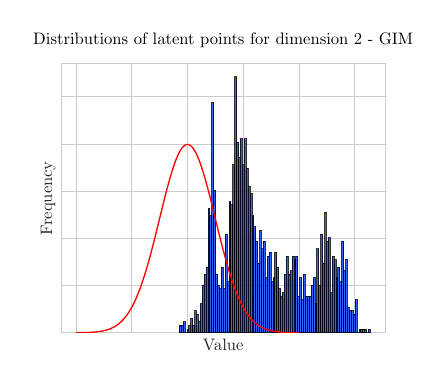
\begin{tikzpicture}[scale=0.6]

\definecolor{blue262255}{RGB}{2,62,255}
\definecolor{darkslategray38}{RGB}{38,38,38}
\definecolor{lightgray204}{RGB}{204,204,204}

\begin{axis}[
axis line style={lightgray204},
tick align=outside,
title={Distributions of latent points for dimension 2 - GIM},
x grid style={lightgray204},
xlabel=\textcolor{darkslategray38}{Value},
xmajorgrids,
xmajorticks=false,
xmin=-4.52819678783417, xmax=7.09213254451752,
xtick style={color=darkslategray38},
y grid style={lightgray204},
ylabel=\textcolor{darkslategray38}{Frequency},
ymajorgrids,
ymajorticks=false,
ymin=0, ymax=0.569871734776329,
ytick style={color=darkslategray38}
]
\draw[draw=black,fill=blue262255,opacity=0.8,line width=0.48pt] (axis cs:-0.29286652803421,0) rectangle (axis cs:-0.224298506975174,0.0155067071316452);
\draw[draw=black,fill=blue262255,opacity=0.8,line width=0.48pt] (axis cs:-0.224298536777496,0) rectangle (axis cs:-0.15573051571846,0.0155067071316452);
\draw[draw=black,fill=blue262255,opacity=0.8,line width=0.48pt] (axis cs:-0.15573051571846,0) rectangle (axis cs:-0.0871624946594238,0.0232600581700369);
\draw[draw=black,fill=blue262255,opacity=0.8,line width=0.48pt] (axis cs:-0.0871624872088432,0) rectangle (axis cs:-0.018594466149807,0);
\draw[draw=black,fill=blue262255,opacity=0.8,line width=0.48pt] (axis cs:-0.018594466149807,0) rectangle (axis cs:0.0499735549092293,0.00775335356582262);
\draw[draw=black,fill=blue262255,opacity=0.8,line width=0.48pt] (axis cs:0.0499735623598099,0) rectangle (axis cs:0.118541583418846,0.0155067071316452);
\draw[draw=black,fill=blue262255,opacity=0.8,line width=0.48pt] (axis cs:0.118541583418846,0) rectangle (axis cs:0.187109604477882,0.0310134142632905);
\draw[draw=black,fill=blue262255,opacity=0.8,line width=0.48pt] (axis cs:0.187109589576721,0) rectangle (axis cs:0.25567764043808,0.0155067037617377);
\draw[draw=black,fill=blue262255,opacity=0.8,line width=0.48pt] (axis cs:0.25567764043808,0) rectangle (axis cs:0.324245661497116,0.0465201213949357);
\draw[draw=black,fill=blue262255,opacity=0.8,line width=0.48pt] (axis cs:0.324245691299438,0) rectangle (axis cs:0.392813712358475,0.0387667678291131);
\draw[draw=black,fill=blue262255,opacity=0.8,line width=0.48pt] (axis cs:0.392813682556152,0) rectangle (axis cs:0.461381703615189,0.0232600606974678);
\draw[draw=black,fill=blue262255,opacity=0.8,line width=0.48pt] (axis cs:0.461381733417511,0) rectangle (axis cs:0.52994978427887,0.0620268285265809);
\draw[draw=black,fill=blue262255,opacity=0.8,line width=0.48pt] (axis cs:0.529949724674225,0) rectangle (axis cs:0.598517715930939,0.100793640164521);
\draw[draw=black,fill=blue262255,opacity=0.8,line width=0.48pt] (axis cs:0.598517775535583,0) rectangle (axis cs:0.667085826396942,0.124053603134653);
\draw[draw=black,fill=blue262255,opacity=0.8,line width=0.48pt] (axis cs:0.667085766792297,0) rectangle (axis cs:0.735653817653656,0.139560303526484);
\draw[draw=black,fill=blue262255,opacity=0.8,line width=0.48pt] (axis cs:0.735653817653656,0) rectangle (axis cs:0.80422180891037,0.263614135814901);
\draw[draw=black,fill=blue262255,opacity=0.8,line width=0.48pt] (axis cs:0.804221868515015,0) rectangle (axis cs:0.872789919376373,0.248107206269305);
\draw[draw=black,fill=blue262255,opacity=0.8,line width=0.48pt] (axis cs:0.872789859771729,0) rectangle (axis cs:0.941357851028442,0.488461486951139);
\draw[draw=black,fill=blue262255,opacity=0.8,line width=0.48pt] (axis cs:0.941357851028442,0) rectangle (axis cs:1.00992584228516,0.302380920493562);
\draw[draw=black,fill=blue262255,opacity=0.8,line width=0.48pt] (axis cs:1.00992584228516,0) rectangle (axis cs:1.07849395275116,0.124053495297775);
\draw[draw=black,fill=blue262255,opacity=0.8,line width=0.48pt] (axis cs:1.07849395275116,0) rectangle (axis cs:1.14706194400787,0.100793640164521);
\draw[draw=black,fill=blue262255,opacity=0.8,line width=0.48pt] (axis cs:1.14706194400787,0) rectangle (axis cs:1.21562993526459,0.0930402832287884);
\draw[draw=black,fill=blue262255,opacity=0.8,line width=0.48pt] (axis cs:1.21562993526459,0) rectangle (axis cs:1.2841979265213,0.139560424843183);
\draw[draw=black,fill=blue262255,opacity=0.8,line width=0.48pt] (axis cs:1.28419780731201,0) rectangle (axis cs:1.35276591777802,0.0930401214733312);
\draw[draw=black,fill=blue262255,opacity=0.8,line width=0.48pt] (axis cs:1.3527660369873,0) rectangle (axis cs:1.42133402824402,0.209340637264774);
\draw[draw=black,fill=blue262255,opacity=0.8,line width=0.48pt] (axis cs:1.42133402824402,0) rectangle (axis cs:1.48990201950073,0.108546997100253);
\draw[draw=black,fill=blue262255,opacity=0.8,line width=0.48pt] (axis cs:1.48990201950073,0) rectangle (axis cs:1.55847001075745,0.279120849686365);
\draw[draw=black,fill=blue262255,opacity=0.8,line width=0.48pt] (axis cs:1.55847001075745,0) rectangle (axis cs:1.62703812122345,0.271367020963883);
\draw[draw=black,fill=blue262255,opacity=0.8,line width=0.48pt] (axis cs:1.62703812122345,0) rectangle (axis cs:1.69560611248016,0.356654419043689);
\draw[draw=black,fill=blue262255,opacity=0.8,line width=0.48pt] (axis cs:1.69560611248016,0) rectangle (axis cs:1.76417410373688,0.542734985501266);
\draw[draw=black,fill=blue262255,opacity=0.8,line width=0.48pt] (axis cs:1.76417398452759,0) rectangle (axis cs:1.83274209499359,0.403173859717768);
\draw[draw=black,fill=blue262255,opacity=0.8,line width=0.48pt] (axis cs:1.83274221420288,0) rectangle (axis cs:1.90131020545959,0.372161132915154);
\draw[draw=black,fill=blue262255,opacity=0.8,line width=0.48pt] (axis cs:1.90131020545959,0) rectangle (axis cs:1.96987819671631,0.410927917593816);
\draw[draw=black,fill=blue262255,opacity=0.8,line width=0.48pt] (axis cs:1.9698783159256,0) rectangle (axis cs:2.0384464263916,0.356654419043689);
\draw[draw=black,fill=blue262255,opacity=0.8,line width=0.48pt] (axis cs:2.03844594955444,0) rectangle (axis cs:2.10701394081116,0.410927917593816);
\draw[draw=black,fill=blue262255,opacity=0.8,line width=0.48pt] (axis cs:2.10701417922974,0) rectangle (axis cs:2.17558217048645,0.348901062107957);
\draw[draw=black,fill=blue262255,opacity=0.8,line width=0.48pt] (axis cs:2.17558217048645,0) rectangle (axis cs:2.24415040016174,0.310133199061454);
\draw[draw=black,fill=blue262255,opacity=0.8,line width=0.48pt] (axis cs:2.24415016174316,0) rectangle (axis cs:2.31271815299988,0.29462756355783);
\draw[draw=black,fill=blue262255,opacity=0.8,line width=0.48pt] (axis cs:2.31271839141846,0) rectangle (axis cs:2.38128638267517,0.248107421943436);
\draw[draw=black,fill=blue262255,opacity=0.8,line width=0.48pt] (axis cs:2.38128614425659,0) rectangle (axis cs:2.44985413551331,0.224847351136239);
\draw[draw=black,fill=blue262255,opacity=0.8,line width=0.48pt] (axis cs:2.44985437393188,0) rectangle (axis cs:2.5184223651886,0.193833923393309);
\draw[draw=black,fill=blue262255,opacity=0.8,line width=0.48pt] (axis cs:2.51842212677002,0) rectangle (axis cs:2.58699011802673,0.147313781778915);
\draw[draw=black,fill=blue262255,opacity=0.8,line width=0.48pt] (axis cs:2.58699035644531,0) rectangle (axis cs:2.65555834770203,0.217093994200506);
\draw[draw=black,fill=blue262255,opacity=0.8,line width=0.48pt] (axis cs:2.65555834770203,0) rectangle (axis cs:2.72412657737732,0.178326589460336);
\draw[draw=black,fill=blue262255,opacity=0.8,line width=0.48pt] (axis cs:2.72412633895874,0) rectangle (axis cs:2.79269433021545,0.193833923393309);
\draw[draw=black,fill=blue262255,opacity=0.8,line width=0.48pt] (axis cs:2.79269456863403,0) rectangle (axis cs:2.86126255989075,0.116300354035986);
\draw[draw=black,fill=blue262255,opacity=0.8,line width=0.48pt] (axis cs:2.86126232147217,0) rectangle (axis cs:2.92983031272888,0.16282049565038);
\draw[draw=black,fill=blue262255,opacity=0.8,line width=0.48pt] (axis cs:2.92983055114746,0) rectangle (axis cs:2.99839854240417,0.170573852586112);
\draw[draw=black,fill=blue262255,opacity=0.8,line width=0.48pt] (axis cs:2.9983983039856,0) rectangle (axis cs:3.06696629524231,0.108546997100253);
\draw[draw=black,fill=blue262255,opacity=0.8,line width=0.48pt] (axis cs:3.06696653366089,0) rectangle (axis cs:3.1355345249176,0.116300354035986);
\draw[draw=black,fill=blue262255,opacity=0.8,line width=0.48pt] (axis cs:3.13553428649902,0) rectangle (axis cs:3.20410227775574,0.170573852586112);
\draw[draw=black,fill=blue262255,opacity=0.8,line width=0.48pt] (axis cs:3.20410251617432,0) rectangle (axis cs:3.27267074584961,0.139559939577654);
\draw[draw=black,fill=blue262255,opacity=0.8,line width=0.48pt] (axis cs:3.27267074584961,0) rectangle (axis cs:3.34123873710632,0.0930402832287884);
\draw[draw=black,fill=blue262255,opacity=0.8,line width=0.48pt] (axis cs:3.34123849868774,0) rectangle (axis cs:3.40980648994446,0.0775335693573237);
\draw[draw=black,fill=blue262255,opacity=0.8,line width=0.48pt] (axis cs:3.40980672836304,0) rectangle (axis cs:3.47837471961975,0.0852869262930561);
\draw[draw=black,fill=blue262255,opacity=0.8,line width=0.48pt] (axis cs:3.47837448120117,0) rectangle (axis cs:3.54694247245789,0.124053710971718);
\draw[draw=black,fill=blue262255,opacity=0.8,line width=0.48pt] (axis cs:3.54694271087646,0) rectangle (axis cs:3.61551070213318,0.16282049565038);
\draw[draw=black,fill=blue262255,opacity=0.8,line width=0.48pt] (axis cs:3.6155104637146,0) rectangle (axis cs:3.68407845497131,0.124053710971718);
\draw[draw=black,fill=blue262255,opacity=0.8,line width=0.48pt] (axis cs:3.68407869338989,0) rectangle (axis cs:3.75264692306519,0.131806609601118);
\draw[draw=black,fill=blue262255,opacity=0.8,line width=0.48pt] (axis cs:3.75264692306519,0) rectangle (axis cs:3.8212149143219,0.16282049565038);
\draw[draw=black,fill=blue262255,opacity=0.8,line width=0.48pt] (axis cs:3.82121467590332,0) rectangle (axis cs:3.88978266716003,0.155067138714647);
\draw[draw=black,fill=blue262255,opacity=0.8,line width=0.48pt] (axis cs:3.88978290557861,0) rectangle (axis cs:3.95835089683533,0.16282049565038);
\draw[draw=black,fill=blue262255,opacity=0.8,line width=0.48pt] (axis cs:3.95835065841675,0) rectangle (axis cs:4.02691841125488,0.0775335693573237);
\draw[draw=black,fill=blue262255,opacity=0.8,line width=0.48pt] (axis cs:4.02691888809204,0) rectangle (axis cs:4.09548711776733,0.116299949648045);
\draw[draw=black,fill=blue262255,opacity=0.8,line width=0.48pt] (axis cs:4.09548759460449,0) rectangle (axis cs:4.16405534744263,0.0697804550560428);
\draw[draw=black,fill=blue262255,opacity=0.8,line width=0.48pt] (axis cs:4.16405487060547,0) rectangle (axis cs:4.23262310028076,0.124053279624582);
\draw[draw=black,fill=blue262255,opacity=0.8,line width=0.48pt] (axis cs:4.23262310028076,0) rectangle (axis cs:4.3011908531189,0.0775338389511586);
\draw[draw=black,fill=blue262255,opacity=0.8,line width=0.48pt] (axis cs:4.3011908531189,0) rectangle (axis cs:4.36975908279419,0.0775332997653636);
\draw[draw=black,fill=blue262255,opacity=0.8,line width=0.48pt] (axis cs:4.36975955963135,0) rectangle (axis cs:4.43832731246948,0.0775338389511586);
\draw[draw=black,fill=blue262255,opacity=0.8,line width=0.48pt] (axis cs:4.43832683563232,0) rectangle (axis cs:4.50689506530762,0.100793289694973);
\draw[draw=black,fill=blue262255,opacity=0.8,line width=0.48pt] (axis cs:4.50689506530762,0) rectangle (axis cs:4.57546329498291,0.116299949648045);
\draw[draw=black,fill=blue262255,opacity=0.8,line width=0.48pt] (axis cs:4.57546329498291,0) rectangle (axis cs:4.64403104782104,0.0620270711609269);
\draw[draw=black,fill=blue262255,opacity=0.8,line width=0.48pt] (axis cs:4.64403104782104,0) rectangle (axis cs:4.71259927749634,0.178326589460336);
\draw[draw=black,fill=blue262255,opacity=0.8,line width=0.48pt] (axis cs:4.7125997543335,0) rectangle (axis cs:4.78116750717163,0.100793990636506);
\draw[draw=black,fill=blue262255,opacity=0.8,line width=0.48pt] (axis cs:4.78116703033447,0) rectangle (axis cs:4.84973526000977,0.209339909366482);
\draw[draw=black,fill=blue262255,opacity=0.8,line width=0.48pt] (axis cs:4.84973526000977,0) rectangle (axis cs:4.9183030128479,0.147314294007201);
\draw[draw=black,fill=blue262255,opacity=0.8,line width=0.48pt] (axis cs:4.9183030128479,0) rectangle (axis cs:4.98687124252319,0.2558598892257);
\draw[draw=black,fill=blue262255,opacity=0.8,line width=0.48pt] (axis cs:4.98687124252319,0) rectangle (axis cs:5.05543947219849,0.193833249413409);
\draw[draw=black,fill=blue262255,opacity=0.8,line width=0.48pt] (axis cs:5.05543994903564,0) rectangle (axis cs:5.12400770187378,0.201587981273012);
\draw[draw=black,fill=blue262255,opacity=0.8,line width=0.48pt] (axis cs:5.12400722503662,0) rectangle (axis cs:5.19257545471191,0.0852866297419);
\draw[draw=black,fill=blue262255,opacity=0.8,line width=0.48pt] (axis cs:5.19257545471191,0) rectangle (axis cs:5.26114320755005,0.162821061797433);
\draw[draw=black,fill=blue262255,opacity=0.8,line width=0.48pt] (axis cs:5.26114320755005,0) rectangle (axis cs:5.32971143722534,0.155066599530727);
\draw[draw=black,fill=blue262255,opacity=0.8,line width=0.48pt] (axis cs:5.3297119140625,0) rectangle (axis cs:5.39827966690063,0.116300758426738);
\draw[draw=black,fill=blue262255,opacity=0.8,line width=0.48pt] (axis cs:5.39827919006348,0) rectangle (axis cs:5.46684741973877,0.139559939577654);
\draw[draw=black,fill=blue262255,opacity=0.8,line width=0.48pt] (axis cs:5.46684741973877,0) rectangle (axis cs:5.5354151725769,0.108547374531622);
\draw[draw=black,fill=blue262255,opacity=0.8,line width=0.48pt] (axis cs:5.5354151725769,0) rectangle (axis cs:5.6039834022522,0.193833249413409);
\draw[draw=black,fill=blue262255,opacity=0.8,line width=0.48pt] (axis cs:5.6039834022522,0) rectangle (axis cs:5.67255163192749,0.131806609601118);
\draw[draw=black,fill=blue262255,opacity=0.8,line width=0.48pt] (axis cs:5.67255210876465,0) rectangle (axis cs:5.74111986160278,0.155067677902317);
\draw[draw=black,fill=blue262255,opacity=0.8,line width=0.48pt] (axis cs:5.74111938476562,0) rectangle (axis cs:5.80968761444092,0.0542733098357545);
\draw[draw=black,fill=blue262255,opacity=0.8,line width=0.48pt] (axis cs:5.80968761444092,0) rectangle (axis cs:5.87825536727905,0.0465203033706952);
\draw[draw=black,fill=blue262255,opacity=0.8,line width=0.48pt] (axis cs:5.87825536727905,0) rectangle (axis cs:5.94682359695435,0.0465199798592182);
\draw[draw=black,fill=blue262255,opacity=0.8,line width=0.48pt] (axis cs:5.9468240737915,0) rectangle (axis cs:6.01539182662964,0.0387669194755793);
\draw[draw=black,fill=blue262255,opacity=0.8,line width=0.48pt] (axis cs:6.01539134979248,0) rectangle (axis cs:6.08395957946777,0.0697799697888272);
\draw[draw=black,fill=blue262255,opacity=0.8,line width=0.48pt] (axis cs:6.08395957946777,0) rectangle (axis cs:6.15252780914307,0);
\draw[draw=black,fill=blue262255,opacity=0.8,line width=0.48pt] (axis cs:6.15252780914307,0) rectangle (axis cs:6.2210955619812,0.00775338389511586);
\draw[draw=black,fill=blue262255,opacity=0.8,line width=0.48pt] (axis cs:6.2210955619812,0) rectangle (axis cs:6.28966379165649,0.00775332997653636);
\draw[draw=black,fill=blue262255,opacity=0.8,line width=0.48pt] (axis cs:6.28966426849365,0) rectangle (axis cs:6.35823202133179,0.00775338389511586);
\draw[draw=black,fill=blue262255,opacity=0.8,line width=0.48pt] (axis cs:6.35823154449463,0) rectangle (axis cs:6.42679977416992,0.00775332997653636);
\draw[draw=black,fill=blue262255,opacity=0.8,line width=0.48pt] (axis cs:6.42679977416992,0) rectangle (axis cs:6.49536752700806,0);
\draw[draw=black,fill=blue262255,opacity=0.8,line width=0.48pt] (axis cs:6.49536752700806,0) rectangle (axis cs:6.56393575668335,0.00775332997653636);
\addplot [thick, red]
table {%
-4 0.000133830225764885
-3.99199199199199 0.000138182046410498
-3.98398398398398 0.000142666228042307
-3.97597597597598 0.000147286481503254
-3.96796796796797 0.000152046611333821
-3.95995995995996 0.000156950517814782
-3.95195195195195 0.00016200219904485
-3.94394394394394 0.00016720575305353
-3.93593593593594 0.000172565379949496
-3.92792792792793 0.00017808538410479
-3.91991991991992 0.000183770176375138
-3.91191191191191 0.000189624276356684
-3.9039039039039 0.000195652314679408
-3.8958958958959 0.000201859035337517
-3.88788788788789 0.000208249298057069
-3.87987987987988 0.000214828080701088
-3.87187187187187 0.000221600481712426
-3.86386386386386 0.0002285717225946
-3.85585585585586 0.000235747150430845
-3.84784784784785 0.000243132240441603
-3.83983983983984 0.000250732598580649
-3.83183183183183 0.000258553964170059
-3.82382382382382 0.000266602212574213
-3.81581581581582 0.000274883357912987
-3.80780780780781 0.000283403555814325
-3.7997997997998 0.000292169106206322
-3.79179179179179 0.000301186456148957
-3.78378378378378 0.0003104622027056
-3.77577577577578 0.000320003095854415
-3.76776776776777 0.000329816041439723
-3.75975975975976 0.000339908104163431
-3.75175175175175 0.00035028651061658
-3.74374374374374 0.000360958652351047
-3.73573573573574 0.000371932088991451
-3.72772772772773 0.000383214551387261
-3.71971971971972 0.000394813944805093
-3.71171171171171 0.000406738352161197
-3.7037037037037 0.000418996037294058
-3.6956956956957 0.00043159544827708
-3.68768768768769 0.00044454522077123
-3.67967967967968 0.000457854181417586
-3.67167167167167 0.000471531351269624
-3.66366366366366 0.000485585949265103
-3.65565565565566 0.000500027395737409
-3.64764764764765 0.000514865315966112
-3.63963963963964 0.000530109543766577
-3.63163163163163 0.000545770125118336
-3.62362362362362 0.000561857321831991
-3.61561561561562 0.00057838161525435
-3.60760760760761 0.000595353710011453
-3.5995995995996 0.000612784537789192
-3.59159159159159 0.000630685261151105
-3.58358358358358 0.000649067277392973
-3.57557557557558 0.000667942222433796
-3.56756756756757 0.000687321974742665
-3.55955955955956 0.000707218659301081
-3.55155155155155 0.000727644651600166
-3.54354354354354 0.000748612581672245
-3.53553553553554 0.000770135338156225
-3.52752752752753 0.000792226072396121
-3.51951951951952 0.00081489820257214
-3.51151151151151 0.000838165417863603
-3.5035035035035 0.000862041682643007
-3.4954954954955 0.000886541240700502
-3.48748748748749 0.00091167861949796
-3.47947947947948 0.000937468634451866
-3.47147147147147 0.000963926393244149
-3.46346346346346 0.000991067300160059
-3.45545545545546 0.0010189070604522
-3.44744744744745 0.00104746168472971
-3.43943943943944 0.0010767474933716
-3.43143143143143 0.00110678112096323
-3.42342342342342 0.00113757952075483
-3.41541541541542 0.00116915996914087
-3.40740740740741 0.00120154007015926
-3.3993993993994 0.00123473776000907
-3.39139139139139 0.00126877131158549
-3.38338338338338 0.00130365933903088
-3.37537537537538 0.00133942080230046
-3.36736736736737 0.00137607501174126
-3.35935935935936 0.001413641632683
-3.35135135135135 0.00145214069003938
-3.34334334334334 0.0014915925729182
-3.33533533533534 0.00153201803923895
-3.32732732732733 0.00157343822035606
-3.31931931931932 0.00161587462568624
-3.31131131131131 0.00165934914733831
-3.3033033033033 0.00170388406474362
-3.2952952952953 0.00174950204928538
-3.28728728728729 0.00179622616892505
-3.27927927927928 0.00184407989282385
-3.27127127127127 0.00189308709595757
-3.26326326326326 0.00194327206372255
-3.25525525525526 0.00199465949653091
-3.24724724724725 0.00204727451439301
-3.23923923923924 0.00210114266148476
-3.23123123123123 0.00215628991069791
-3.22322322322322 0.00221274266817093
-3.21521521521522 0.00227052777779815
-3.20720720720721 0.00232967252571501
-3.1991991991992 0.00239020464475689
-3.19119119119119 0.00245215231888918
-3.18318318318318 0.00251554418760605
-3.17517517517518 0.00258040935029545
-3.16716716716717 0.00264677737056774
-3.15915915915916 0.00271467828054534
-3.15115115115115 0.00278414258511061
-3.14314314314314 0.00285520126610952
-3.13513513513514 0.00292788578650791
-3.12712712712713 0.00300222809449793
-3.11911911911912 0.00307826062755151
-3.11111111111111 0.00315601631641804
-3.1031031031031 0.00323552858906328
-3.0950950950951 0.00331683137454643
-3.08708708708709 0.00339995910683238
-3.07907907907908 0.00348494672853595
-3.07107107107107 0.00357182969459489
-3.06306306306306 0.00366064397586864
-3.05505505505506 0.00375142606265932
-3.04704704704705 0.00384421296815189
-3.03903903903904 0.00393904223176991
-3.03103103103103 0.00403595192244368
-3.02302302302302 0.0041349806417872
-3.01501501501502 0.00423616752718052
-3.00700700700701 0.00433955225475399
-2.998998998999 0.00444517504227068
-2.99099099099099 0.00455307665190355
-2.98298298298298 0.00466329839290368
-2.97497497497497 0.00477588212415564
-2.96696696696697 0.00489087025661667
-2.95895895895896 0.00500830575563558
-2.95095095095095 0.00512823214314763
-2.94294294294294 0.00525069349974172
-2.93493493493493 0.00537573446659573
-2.92692692692693 0.00550340024727644
-2.91891891891892 0.00563373660939975
-2.91091091091091 0.0057667898861475
-2.9029029029029 0.00590260697763674
-2.89489489489489 0.00604123535213746
-2.88688688688689 0.00618272304713484
-2.87887887887888 0.00632711867023164
-2.87087087087087 0.00647447139988703
-2.86286286286286 0.00662483098598741
-2.85485485485485 0.0067782477502453
-2.84684684684685 0.0069347725864219
-2.83883883883884 0.00709445696036946
-2.83083083083083 0.00725735290988893
-2.82282282282282 0.00742351304439893
-2.81481481481481 0.00759299054441176
-2.80680680680681 0.0077658391608121
-2.7987987987988 0.00794211321393437
-2.79079079079079 0.00812186759243432
-2.78278278278278 0.00830515775195071
-2.77477477477477 0.00849203971355293
-2.76676676676677 0.00868257006197001
-2.75875875875876 0.00887680594359712
-2.75075075075075 0.00907480506427511
-2.74274274274274 0.00927662568683898
-2.73473473473473 0.00948232662843099
-2.72672672672673 0.00969196725757422
-2.71871871871872 0.00990560749100246
-2.71071071071071 0.0101233077902421
-2.7027027027027 0.0103451291579421
-2.69469469469469 0.0105711331339476
-2.68668668668669 0.0108013817911136
-2.67867867867868 0.011035937730854
-2.67067067067067 0.0112748640784219
-2.66266266266266 0.0115182244779185
-2.65465465465465 0.0117660830870247
-2.64664664664665 0.0120185045714526
-2.63863863863864 0.0122755540991133
-2.63063063063063 0.0125372973339956
-2.62262262262262 0.0128038004297541
-2.61461461461461 0.0130751300230007
-2.60660660660661 0.0133513532262973
-2.5985985985986 0.0136325376208454
-2.59059059059059 0.0139187512488692
-2.58258258258258 0.014210062605689
-2.57457457457457 0.0145065406314803
-2.56656656656657 0.0148082547027168
-2.55855855855856 0.0151152746232934
-2.55055055055055 0.0154276706153247
-2.54254254254254 0.0157455133096184
-2.53453453453453 0.0160688737358178
-2.52652652652653 0.016397823312213
-2.51851851851852 0.0167324338352151
-2.51051051051051 0.0170727774684938
-2.5025025025025 0.0174189267317727
-2.49449449449449 0.0177709544892815
-2.48648648648649 0.0181289339378627
-2.47847847847848 0.0184929385947284
-2.47047047047047 0.0188630422848682
-2.46246246246246 0.0192393191281025
-2.45445445445445 0.0196218435257817
-2.44644644644645 0.0200106901471285
-2.43843843843844 0.020405933915221
-2.43043043043043 0.0208076499926159
-2.42242242242242 0.0212159137666093
-2.41441441441441 0.0216308008341344
-2.40640640640641 0.0220523869862944
-2.3983983983984 0.0224807481925294
-2.39039039039039 0.022915960584417
-2.38238238238238 0.0233581004391047
-2.37437437437437 0.023807244162374
-2.36636636636637 0.0242634682713357
-2.35835835835836 0.0247268493767558
-2.35035035035035 0.0251974641650118
-2.34234234234234 0.0256753893796796
-2.33433433433433 0.0261607018027501
-2.32632632632633 0.0266534782354775
-2.31831831831832 0.0271537954788581
-2.31031031031031 0.0276617303137407
-2.3023023023023 0.0281773594805703
-2.29429429429429 0.0287007596587648
-2.28628628628629 0.0292320074457259
-2.27827827827828 0.029771179335487
-2.27027027027027 0.0303183516969979
-2.26226226226226 0.0308736007520491
-2.25425425425425 0.0314370025528369
-2.24624624624625 0.0320086329591723
-2.23823823823824 0.0325885676153351
-2.23023023023023 0.0331768819265761
-2.22222222222222 0.0337736510352706
-2.21421421421421 0.0343789497967251
-2.20620620620621 0.0349928527546413
-2.1981981981982 0.0356154341162401
-2.19019019019019 0.0362467677270497
-2.18218218218218 0.0368869270453615
-2.17417417417417 0.0375359851163567
-2.16616616616617 0.03819401454591
-2.15815815815816 0.0388610874740724
-2.15015015015015 0.03953727554824
-2.14214214214214 0.0402226498960119
-2.13413413413413 0.0409172810977437
-2.12612612612613 0.0416212391588003
-2.11811811811812 0.0423345934815158
-2.11011011011011 0.0430574128368641
-2.1021021021021 0.043789765335848
-2.09409409409409 0.0445317184006117
-2.08608608608609 0.0452833387352837
-2.07807807807808 0.0460446922965577
-2.07007007007007 0.0468158442640166
-2.06206206206206 0.0475968590102091
-2.05405405405405 0.0483878000704834
-2.04604604604605 0.0491887301125894
-2.03803803803804 0.0499997109060533
-2.03003003003003 0.0508208032913361
-2.02202202202202 0.0516520671487823
-2.01401401401401 0.0524935613673682
-2.00600600600601 0.053345343813258
-1.997997997998 0.0542074712981785
-1.98998998998999 0.0550799995476186
-1.98198198198198 0.0559629831688668
-1.97397397397397 0.0568564756188931
-1.96596596596597 0.0577605291720876
-1.95795795795796 0.0586751948878651
-1.94994994994995 0.0596005225781457
-1.94194194194194 0.0605365607747232
-1.93393393393393 0.0614833566965309
-1.92592592592593 0.062440956216817
-1.91791791791792 0.06340940383024
-1.90990990990991 0.0643887426198963
-1.9019019019019 0.0653790142242912
-1.89389389389389 0.0663802588042656
-1.88588588588589 0.0673925150098903
-1.87787787787788 0.0684158199473405
-1.86986986986987 0.0694502091457625
-1.86186186186186 0.0704957165241465
-1.85385385385385 0.0715523743582165
-1.84584584584585 0.0726202132473521
-1.83783783783784 0.0736992620815557
-1.82982982982983 0.0747895480084762
-1.82182182182182 0.0758910964005057
-1.81381381381381 0.0770039308219614
-1.80580580580581 0.0781280729963669
-1.7977977977978 0.0792635427738473
-1.78978978978979 0.0804103580986525
-1.78178178178178 0.0815685349768227
-1.77377377377377 0.0827380874440109
-1.76576576576577 0.0839190275334777
-1.75775775775776 0.0851113652442723
-1.74974974974975 0.086315108509615
-1.74174174174174 0.0875302631654975
-1.73373373373373 0.0887568329195139
-1.72572572572573 0.0899948193199405
-1.71771771771772 0.0912442217250772
-1.70970970970971 0.0925050372728685
-1.7017017017017 0.0937772608508177
-1.69369369369369 0.0950608850662112
-1.68568568568569 0.0963559002166691
-1.67767767767768 0.0976622942610365
-1.66966966966967 0.0989800527906321
-1.66166166166166 0.100309159000872
-1.65365365365365 0.10164959366328
-1.64564564564565 0.103001335097907
-1.63763763763764 0.10436435914617
-1.62962962962963 0.105738639144131
-1.62162162162162 0.107124145896225
-1.61361361361361 0.108520847649465
-1.60560560560561 0.10992871006813
-1.5975975975976 0.111347696208955
-1.58958958958959 0.112777766496842
-1.58158158158158 0.114218878701105
-1.57357357357357 0.115670987912262
-1.56556556556557 0.117134046519405
-1.55755755755756 0.11860800418814
-1.54954954954955 0.120092807839133
-1.54154154154154 0.121588401627275
-1.53353353353353 0.123094726921466
-1.52552552552553 0.124611722285057
-1.51751751751752 0.12613932345695
-1.50950950950951 0.127677463333369
-1.5015015015015 0.129226071950339
-1.49349349349349 0.130785076466857
-1.48548548548549 0.132354401148798
-1.47747747747748 0.133933967353555
-1.46946946946947 0.13552369351543
-1.46146146146146 0.137123495131801
-1.45345345345345 0.13873328475006
-1.44544544544545 0.140352971955359
-1.43743743743744 0.141982463359159
-1.42942942942943 0.143621662588612
-1.42142142142142 0.14527047027677
-1.41341341341341 0.146928784053658
-1.40540540540541 0.148596498538208
-1.3973973973974 0.150273505331067
-1.38938938938939 0.151959693008306
-1.38138138138138 0.153654947116025
-1.37337337337337 0.155359150165875
-1.36536536536537 0.157072181631514
-1.35735735735736 0.158793917945997
-1.34934934934935 0.160524232500121
-1.34134134134134 0.16226299564173
-1.33333333333333 0.164010074675994
-1.32532532532533 0.165765333866673
-1.31731731731732 0.167528634438376
-1.30930930930931 0.169299834579821
-1.3013013013013 0.17107878944811
-1.29329329329329 0.172865351174024
-1.28528528528529 0.174659368868355
-1.27727727727728 0.176460688629273
-1.26926926926927 0.178269153550739
-1.26126126126126 0.180084603731981
-1.25325325325325 0.181906876288021
-1.24524524524525 0.183735805361283
-1.23723723723724 0.185571222134271
-1.22922922922923 0.187412954843324
-1.22122122122122 0.18926082879347
-1.21321321321321 0.191114666374361
-1.20520520520521 0.192974287077311
-1.1971971971972 0.194839507513435
-1.18918918918919 0.19671014143289
-1.18118118118118 0.198585999745227
-1.17317317317317 0.200466890540856
-1.16516516516517 0.202352619113618
-1.15715715715716 0.204242987984477
-1.14914914914915 0.206137796926331
-1.14114114114114 0.208036842989938
-1.13313313313313 0.209939920530956
-1.12512512512513 0.21184682123811
-1.11711711711712 0.21375733416247
-1.10910910910911 0.215671245747847
-1.1011011011011 0.217588339862305
-1.09309309309309 0.219508397830784
-1.08508508508509 0.221431198468836
-1.07707707707708 0.223356518117463
-1.06906906906907 0.225284130679063
-1.06106106106106 0.22721380765447
-1.05305305305305 0.229145318181096
-1.04504504504505 0.231078429072154
-1.03703703703704 0.233012904856966
-1.02902902902903 0.234948507822352
-1.02102102102102 0.236884998055083
-1.01301301301301 0.238822133485401
-1.00500500500501 0.24075966993159
-0.996996996996997 0.242697361145593
-0.988988988988989 0.244634958859672
-0.980980980980981 0.246572212834085
-0.972972972972973 0.248508870905785
-0.964964964964965 0.250444679038131
-0.956956956956957 0.252379381371581
-0.948948948948949 0.254312720275385
-0.940940940940941 0.256244436400228
-0.932932932932933 0.258174268731856
-0.924924924924925 0.260101954645624
-0.916916916916917 0.262027229961987
-0.908908908908909 0.263949829002911
-0.900900900900901 0.265869484649172
-0.892892892892893 0.267785928398552
-0.884884884884885 0.269698890424904
-0.876876876876877 0.271608099638066
-0.868868868868869 0.273513283744617
-0.860860860860861 0.275414169309444
-0.852852852852853 0.277310481818125
-0.844844844844845 0.279201945740075
-0.836836836836837 0.281088284592474
-0.828828828828829 0.28296922100493
-0.820820820820821 0.284844476784867
-0.812812812812813 0.286713772983616
-0.804804804804805 0.288576829963198
-0.796796796796797 0.290433367463758
-0.788788788788789 0.292283104671645
-0.780780780780781 0.294125760288111
-0.772772772772773 0.295961052598604
-0.764764764764765 0.29778869954263
-0.756756756756757 0.299608418784177
-0.748748748748749 0.301419927782648
-0.740740740740741 0.303222943864308
-0.732732732732733 0.305017184294205
-0.724724724724725 0.306802366348536
-0.716716716716717 0.308578207387456
-0.708708708708709 0.310344424928268
-0.700700700700701 0.312100736719007
-0.692692692692693 0.313846860812361
-0.684684684684685 0.31558251563992
-0.676676676676677 0.317307420086723
-0.668668668668669 0.319021293566066
-0.660660660660661 0.320723856094559
-0.652652652652653 0.322414828367396
-0.644644644644645 0.324093931833804
-0.636636636636636 0.325760888772662
-0.628628628628629 0.327415422368237
-0.620620620620621 0.329057256786028
-0.612612612612613 0.330686117248681
-0.604604604604605 0.33230173011195
-0.596596596596596 0.333903822940662
-0.588588588588589 0.335492124584683
-0.580580580580581 0.337066365254824
-0.572572572572573 0.338626276598684
-0.564564564564565 0.340171591776383
-0.556556556556556 0.341702045536168
-0.548548548548549 0.343217374289848
-0.54054054054054 0.344717316188045
-0.532532532532533 0.346201611195215
-0.524524524524525 0.347670001164422
-0.516516516516516 0.349122229911825
-0.508508508508509 0.350558043290856
-0.5005005005005 0.351977189266054
-0.492492492492492 0.353379417986526
-0.484484484484485 0.354764481859011
-0.476476476476476 0.356132135620502
-0.468468468468469 0.357482136410418
-0.46046046046046 0.358814243842273
-0.452452452452452 0.360128220074839
-0.444444444444445 0.361423829882744
-0.436436436436436 0.362700840726495
-0.428428428428429 0.363959022821904
-0.42042042042042 0.365198149208855
-0.412412412412412 0.366417995819425
-0.404404404404405 0.3676183415453
-0.396396396396396 0.368798968304465
-0.388388388388389 0.369959661107154
-0.38038038038038 0.37110020812101
-0.372372372372372 0.372220400735444
-0.364364364364365 0.373320033625156
-0.356356356356356 0.374398904812801
-0.348348348348348 0.375456815730761
-0.34034034034034 0.376493571282005
-0.332332332332332 0.377508979900006
-0.324324324324325 0.378502853607702
-0.316316316316316 0.379475008075448
-0.308308308308308 0.380425262677969
-0.3003003003003 0.38135344055026
-0.292292292292292 0.382259368642425
-0.284284284284285 0.38314287777343
-0.276276276276276 0.384003802683735
-0.268268268268268 0.3848419820868
-0.26026026026026 0.385657258719425
-0.252252252252252 0.386449479390916
-0.244244244244244 0.387218495031049
-0.236236236236236 0.387964160736805
-0.228228228228228 0.38868633581787
-0.22022022022022 0.389384883840873
-0.212212212212212 0.390059672672329
-0.204204204204204 0.390710574520297
-0.196196196196196 0.391337465974705
-0.188188188188188 0.39194022804635
-0.18018018018018 0.392518746204527
-0.172172172172172 0.393072910413305
-0.164164164164164 0.393602615166401
-0.156156156156156 0.394107759520658
-0.148148148148148 0.394588247128102
-0.14014014014014 0.395043986266573
-0.132132132132132 0.3954748898689
-0.124124124124124 0.395880875550626
-0.116116116116116 0.396261865636259
-0.108108108108108 0.396617787184037
-0.1001001001001 0.396948572009207
-0.0920920920920922 0.397254156705792
-0.084084084084084 0.397534482666846
-0.0760760760760761 0.39778949610319
-0.0680680680680683 0.39801914806061
-0.06006006006006 0.398223394435522
-0.0520520520520522 0.398402195989086
-0.0440440440440439 0.398555518359772
-0.0360360360360361 0.398683332074364
-0.0280280280280278 0.398785612557403
-0.02002002002002 0.398862340139061
-0.0120120120120122 0.398913500061449
-0.00400400400400391 0.398939082483343
0.00400400400400436 0.398939082483343
0.0120120120120122 0.398913500061449
0.02002002002002 0.398862340139061
0.0280280280280278 0.398785612557403
0.0360360360360357 0.398683332074364
0.0440440440440444 0.398555518359772
0.0520520520520522 0.398402195989086
0.06006006006006 0.398223394435522
0.0680680680680679 0.39801914806061
0.0760760760760757 0.39778949610319
0.0840840840840844 0.397534482666846
0.0920920920920922 0.397254156705792
0.1001001001001 0.396948572009207
0.108108108108108 0.396617787184037
0.116116116116116 0.396261865636259
0.124124124124124 0.395880875550626
0.132132132132132 0.3954748898689
0.14014014014014 0.395043986266573
0.148148148148148 0.394588247128102
0.156156156156156 0.394107759520658
0.164164164164164 0.393602615166401
0.172172172172172 0.393072910413305
0.18018018018018 0.392518746204527
0.188188188188188 0.39194022804635
0.196196196196196 0.391337465974705
0.204204204204204 0.390710574520297
0.212212212212212 0.390059672672329
0.22022022022022 0.389384883840873
0.228228228228228 0.388686335817871
0.236236236236236 0.387964160736805
0.244244244244245 0.387218495031049
0.252252252252252 0.386449479390916
0.26026026026026 0.385657258719425
0.268268268268268 0.3848419820868
0.276276276276276 0.384003802683735
0.284284284284285 0.38314287777343
0.292292292292292 0.382259368642425
0.3003003003003 0.38135344055026
0.308308308308308 0.380425262677969
0.316316316316316 0.379475008075448
0.324324324324325 0.378502853607702
0.332332332332332 0.377508979900006
0.34034034034034 0.376493571282005
0.348348348348348 0.375456815730762
0.356356356356356 0.374398904812801
0.364364364364365 0.373320033625156
0.372372372372372 0.372220400735444
0.38038038038038 0.37110020812101
0.388388388388388 0.369959661107154
0.396396396396397 0.368798968304465
0.404404404404405 0.3676183415453
0.412412412412412 0.366417995819425
0.42042042042042 0.365198149208855
0.428428428428428 0.363959022821904
0.436436436436437 0.362700840726495
0.444444444444445 0.361423829882744
0.452452452452452 0.360128220074839
0.46046046046046 0.358814243842273
0.468468468468468 0.357482136410418
0.476476476476477 0.356132135620502
0.484484484484485 0.354764481859011
0.492492492492492 0.353379417986526
0.5005005005005 0.351977189266054
0.508508508508508 0.350558043290856
0.516516516516517 0.349122229911825
0.524524524524525 0.347670001164422
0.532532532532533 0.346201611195215
0.54054054054054 0.344717316188045
0.548548548548548 0.343217374289848
0.556556556556557 0.341702045536168
0.564564564564565 0.340171591776383
0.572572572572573 0.338626276598684
0.58058058058058 0.337066365254824
0.588588588588588 0.335492124584683
0.596596596596597 0.333903822940662
0.604604604604605 0.33230173011195
0.612612612612613 0.330686117248681
0.62062062062062 0.329057256786028
0.628628628628628 0.327415422368237
0.636636636636637 0.325760888772662
0.644644644644645 0.324093931833804
0.652652652652653 0.322414828367396
0.66066066066066 0.32072385609456
0.668668668668668 0.319021293566066
0.676676676676677 0.317307420086723
0.684684684684685 0.31558251563992
0.692692692692693 0.313846860812361
0.7007007007007 0.312100736719007
0.708708708708708 0.310344424928268
0.716716716716717 0.308578207387456
0.724724724724725 0.306802366348536
0.732732732732733 0.305017184294205
0.74074074074074 0.303222943864308
0.748748748748748 0.301419927782648
0.756756756756757 0.299608418784177
0.764764764764765 0.29778869954263
0.772772772772773 0.295961052598604
0.780780780780781 0.294125760288111
0.788788788788788 0.292283104671645
0.796796796796797 0.290433367463758
0.804804804804805 0.288576829963198
0.812812812812813 0.286713772983616
0.820820820820821 0.284844476784867
0.828828828828828 0.282969221004931
0.836836836836837 0.281088284592474
0.844844844844845 0.279201945740075
0.852852852852853 0.277310481818125
0.860860860860861 0.275414169309444
0.868868868868869 0.273513283744617
0.876876876876877 0.271608099638066
0.884884884884885 0.269698890424904
0.892892892892893 0.267785928398552
0.900900900900901 0.265869484649172
0.908908908908909 0.263949829002911
0.916916916916917 0.262027229961987
0.924924924924925 0.260101954645624
0.932932932932933 0.258174268731856
0.940940940940941 0.256244436400228
0.948948948948949 0.254312720275384
0.956956956956957 0.252379381371581
0.964964964964965 0.250444679038131
0.972972972972973 0.248508870905785
0.980980980980981 0.246572212834085
0.988988988988989 0.244634958859672
0.996996996996997 0.242697361145593
1.00500500500501 0.24075966993159
1.01301301301301 0.238822133485401
1.02102102102102 0.236884998055083
1.02902902902903 0.234948507822352
1.03703703703704 0.233012904856966
1.04504504504505 0.231078429072154
1.05305305305305 0.229145318181096
1.06106106106106 0.22721380765447
1.06906906906907 0.225284130679062
1.07707707707708 0.223356518117463
1.08508508508509 0.221431198468836
1.09309309309309 0.219508397830784
1.1011011011011 0.217588339862305
1.10910910910911 0.215671245747847
1.11711711711712 0.21375733416247
1.12512512512513 0.21184682123811
1.13313313313313 0.209939920530956
1.14114114114114 0.208036842989938
1.14914914914915 0.206137796926331
1.15715715715716 0.204242987984477
1.16516516516517 0.202352619113618
1.17317317317317 0.200466890540856
1.18118118118118 0.198585999745228
1.18918918918919 0.19671014143289
1.1971971971972 0.194839507513435
1.20520520520521 0.192974287077311
1.21321321321321 0.191114666374361
1.22122122122122 0.18926082879347
1.22922922922923 0.187412954843324
1.23723723723724 0.185571222134271
1.24524524524525 0.183735805361283
1.25325325325325 0.181906876288021
1.26126126126126 0.180084603731981
1.26926926926927 0.178269153550739
1.27727727727728 0.176460688629273
1.28528528528529 0.174659368868355
1.29329329329329 0.172865351174024
1.3013013013013 0.17107878944811
1.30930930930931 0.169299834579821
1.31731731731732 0.167528634438376
1.32532532532533 0.165765333866673
1.33333333333333 0.164010074675994
1.34134134134134 0.16226299564173
1.34934934934935 0.160524232500121
1.35735735735736 0.158793917945997
1.36536536536537 0.157072181631514
1.37337337337337 0.155359150165875
1.38138138138138 0.153654947116025
1.38938938938939 0.151959693008306
1.3973973973974 0.150273505331067
1.40540540540541 0.148596498538208
1.41341341341341 0.146928784053658
1.42142142142142 0.14527047027677
1.42942942942943 0.143621662588612
1.43743743743744 0.141982463359159
1.44544544544545 0.140352971955359
1.45345345345345 0.13873328475006
1.46146146146146 0.137123495131801
1.46946946946947 0.13552369351543
1.47747747747748 0.133933967353555
1.48548548548549 0.132354401148798
1.49349349349349 0.130785076466857
1.5015015015015 0.129226071950339
1.50950950950951 0.127677463333369
1.51751751751752 0.12613932345695
1.52552552552553 0.124611722285057
1.53353353353353 0.123094726921466
1.54154154154154 0.121588401627275
1.54954954954955 0.120092807839133
1.55755755755756 0.11860800418814
1.56556556556557 0.117134046519405
1.57357357357357 0.115670987912262
1.58158158158158 0.114218878701105
1.58958958958959 0.112777766496842
1.5975975975976 0.111347696208955
1.60560560560561 0.10992871006813
1.61361361361361 0.108520847649465
1.62162162162162 0.107124145896225
1.62962962962963 0.105738639144131
1.63763763763764 0.10436435914617
1.64564564564565 0.103001335097907
1.65365365365365 0.10164959366328
1.66166166166166 0.100309159000872
1.66966966966967 0.0989800527906321
1.67767767767768 0.0976622942610365
1.68568568568569 0.0963559002166692
1.69369369369369 0.0950608850662112
1.7017017017017 0.0937772608508176
1.70970970970971 0.0925050372728685
1.71771771771772 0.0912442217250772
1.72572572572573 0.0899948193199405
1.73373373373373 0.088756832919514
1.74174174174174 0.0875302631654974
1.74974974974975 0.086315108509615
1.75775775775776 0.0851113652442723
1.76576576576577 0.0839190275334778
1.77377377377377 0.082738087444011
1.78178178178178 0.0815685349768226
1.78978978978979 0.0804103580986525
1.7977977977978 0.0792635427738473
1.80580580580581 0.0781280729963669
1.81381381381381 0.0770039308219615
1.82182182182182 0.0758910964005057
1.82982982982983 0.0747895480084762
1.83783783783784 0.0736992620815557
1.84584584584585 0.0726202132473522
1.85385385385385 0.0715523743582165
1.86186186186186 0.0704957165241465
1.86986986986987 0.0694502091457625
1.87787787787788 0.0684158199473405
1.88588588588589 0.0673925150098903
1.89389389389389 0.0663802588042655
1.9019019019019 0.0653790142242912
1.90990990990991 0.0643887426198963
1.91791791791792 0.06340940383024
1.92592592592593 0.0624409562168171
1.93393393393393 0.0614833566965309
1.94194194194194 0.0605365607747232
1.94994994994995 0.0596005225781457
1.95795795795796 0.0586751948878651
1.96596596596597 0.0577605291720876
1.97397397397397 0.056856475618893
1.98198198198198 0.0559629831688668
1.98998998998999 0.0550799995476186
1.997997997998 0.0542074712981785
2.00600600600601 0.0533453438132581
2.01401401401401 0.0524935613673681
2.02202202202202 0.0516520671487823
2.03003003003003 0.0508208032913361
2.03803803803804 0.0499997109060533
2.04604604604605 0.0491887301125894
2.05405405405405 0.0483878000704834
2.06206206206206 0.0475968590102091
2.07007007007007 0.0468158442640166
2.07807807807808 0.0460446922965577
2.08608608608609 0.0452833387352837
2.09409409409409 0.0445317184006117
2.1021021021021 0.043789765335848
2.11011011011011 0.0430574128368641
2.11811811811812 0.0423345934815158
2.12612612612613 0.0416212391588004
2.13413413413413 0.0409172810977437
2.14214214214214 0.0402226498960119
2.15015015015015 0.03953727554824
2.15815815815816 0.0388610874740724
2.16616616616617 0.03819401454591
2.17417417417417 0.0375359851163567
2.18218218218218 0.0368869270453615
2.19019019019019 0.0362467677270497
2.1981981981982 0.0356154341162401
2.20620620620621 0.0349928527546413
2.21421421421421 0.0343789497967251
2.22222222222222 0.0337736510352706
2.23023023023023 0.0331768819265761
2.23823823823824 0.0325885676153351
2.24624624624625 0.0320086329591724
2.25425425425425 0.0314370025528369
2.26226226226226 0.0308736007520491
2.27027027027027 0.0303183516969979
2.27827827827828 0.029771179335487
2.28628628628629 0.0292320074457259
2.29429429429429 0.0287007596587648
2.3023023023023 0.0281773594805703
2.31031031031031 0.0276617303137407
2.31831831831832 0.0271537954788581
2.32632632632633 0.0266534782354776
2.33433433433433 0.0261607018027501
2.34234234234234 0.0256753893796796
2.35035035035035 0.0251974641650118
2.35835835835836 0.0247268493767558
2.36636636636637 0.0242634682713357
2.37437437437437 0.023807244162374
2.38238238238238 0.0233581004391047
2.39039039039039 0.022915960584417
2.3983983983984 0.0224807481925294
2.40640640640641 0.0220523869862944
2.41441441441441 0.0216308008341344
2.42242242242242 0.0212159137666093
2.43043043043043 0.0208076499926159
2.43843843843844 0.020405933915221
2.44644644644645 0.0200106901471285
2.45445445445445 0.0196218435257817
2.46246246246246 0.0192393191281025
2.47047047047047 0.0188630422848682
2.47847847847848 0.0184929385947284
2.48648648648649 0.0181289339378626
2.49449449449449 0.0177709544892815
2.5025025025025 0.0174189267317727
2.51051051051051 0.0170727774684938
2.51851851851852 0.0167324338352152
2.52652652652653 0.016397823312213
2.53453453453453 0.0160688737358178
2.54254254254254 0.0157455133096184
2.55055055055055 0.0154276706153247
2.55855855855856 0.0151152746232934
2.56656656656657 0.0148082547027168
2.57457457457457 0.0145065406314803
2.58258258258258 0.014210062605689
2.59059059059059 0.0139187512488692
2.5985985985986 0.0136325376208454
2.60660660660661 0.0133513532262973
2.61461461461461 0.0130751300230007
2.62262262262262 0.0128038004297541
2.63063063063063 0.0125372973339956
2.63863863863864 0.0122755540991133
2.64664664664665 0.0120185045714526
2.65465465465465 0.0117660830870247
2.66266266266266 0.0115182244779185
2.67067067067067 0.0112748640784219
2.67867867867868 0.011035937730854
2.68668668668669 0.0108013817911136
2.69469469469469 0.0105711331339476
2.7027027027027 0.0103451291579421
2.71071071071071 0.0101233077902421
2.71871871871872 0.00990560749100247
2.72672672672673 0.00969196725757422
2.73473473473473 0.00948232662843099
2.74274274274274 0.00927662568683898
2.75075075075075 0.00907480506427511
2.75875875875876 0.00887680594359712
2.76676676676677 0.00868257006197001
2.77477477477477 0.00849203971355293
2.78278278278278 0.00830515775195071
2.79079079079079 0.00812186759243432
2.7987987987988 0.00794211321393438
2.80680680680681 0.0077658391608121
2.81481481481481 0.00759299054441176
2.82282282282282 0.00742351304439893
2.83083083083083 0.00725735290988893
2.83883883883884 0.00709445696036947
2.84684684684685 0.0069347725864219
2.85485485485485 0.0067782477502453
2.86286286286286 0.00662483098598741
2.87087087087087 0.00647447139988703
2.87887887887888 0.00632711867023165
2.88688688688689 0.00618272304713484
2.89489489489489 0.00604123535213746
2.9029029029029 0.00590260697763674
2.91091091091091 0.0057667898861475
2.91891891891892 0.00563373660939975
2.92692692692693 0.00550340024727644
2.93493493493493 0.00537573446659573
2.94294294294294 0.00525069349974172
2.95095095095095 0.00512823214314764
2.95895895895896 0.00500830575563558
2.96696696696697 0.00489087025661667
2.97497497497497 0.00477588212415564
2.98298298298298 0.00466329839290368
2.99099099099099 0.00455307665190356
2.998998998999 0.00444517504227067
3.00700700700701 0.00433955225475399
3.01501501501502 0.00423616752718052
3.02302302302302 0.0041349806417872
3.03103103103103 0.00403595192244368
3.03903903903904 0.00393904223176991
3.04704704704705 0.00384421296815189
3.05505505505506 0.00375142606265932
3.06306306306306 0.00366064397586864
3.07107107107107 0.00357182969459489
3.07907907907908 0.00348494672853594
3.08708708708709 0.00339995910683238
3.0950950950951 0.00331683137454643
3.1031031031031 0.00323552858906328
3.11111111111111 0.00315601631641805
3.11911911911912 0.00307826062755151
3.12712712712713 0.00300222809449793
3.13513513513514 0.00292788578650791
3.14314314314314 0.00285520126610952
3.15115115115115 0.00278414258511062
3.15915915915916 0.00271467828054533
3.16716716716717 0.00264677737056774
3.17517517517518 0.00258040935029545
3.18318318318318 0.00251554418760605
3.19119119119119 0.00245215231888919
3.1991991991992 0.00239020464475689
3.20720720720721 0.00232967252571501
3.21521521521522 0.00227052777779815
3.22322322322322 0.00221274266817093
3.23123123123123 0.00215628991069792
3.23923923923924 0.00210114266148476
3.24724724724725 0.00204727451439301
3.25525525525526 0.00199465949653091
3.26326326326326 0.00194327206372255
3.27127127127127 0.00189308709595757
3.27927927927928 0.00184407989282385
3.28728728728729 0.00179622616892505
3.2952952952953 0.00174950204928538
3.3033033033033 0.00170388406474362
3.31131131131131 0.00165934914733832
3.31931931931932 0.00161587462568624
3.32732732732733 0.00157343822035606
3.33533533533534 0.00153201803923895
3.34334334334334 0.0014915925729182
3.35135135135135 0.00145214069003938
3.35935935935936 0.001413641632683
3.36736736736737 0.00137607501174126
3.37537537537538 0.00133942080230046
3.38338338338338 0.00130365933903089
3.39139139139139 0.00126877131158549
3.3993993993994 0.00123473776000907
3.40740740740741 0.00120154007015926
3.41541541541542 0.00116915996914087
3.42342342342342 0.00113757952075483
3.43143143143143 0.00110678112096324
3.43943943943944 0.0010767474933716
3.44744744744745 0.00104746168472971
3.45545545545546 0.0010189070604522
3.46346346346346 0.000991067300160061
3.47147147147147 0.000963926393244148
3.47947947947948 0.000937468634451866
3.48748748748749 0.00091167861949796
3.4954954954955 0.000886541240700502
3.5035035035035 0.000862041682643008
3.51151151151151 0.000838165417863601
3.51951951951952 0.00081489820257214
3.52752752752753 0.000792226072396121
3.53553553553554 0.000770135338156225
3.54354354354354 0.000748612581672247
3.55155155155155 0.000727644651600165
3.55955955955956 0.000707218659301081
3.56756756756757 0.000687321974742665
3.57557557557558 0.000667942222433796
3.58358358358358 0.000649067277392974
3.59159159159159 0.000630685261151104
3.5995995995996 0.000612784537789192
3.60760760760761 0.000595353710011453
3.61561561561562 0.00057838161525435
3.62362362362362 0.000561857321831992
3.63163163163163 0.000545770125118335
3.63963963963964 0.000530109543766577
3.64764764764765 0.000514865315966112
3.65565565565566 0.000500027395737409
3.66366366366366 0.000485585949265104
3.67167167167167 0.000471531351269623
3.67967967967968 0.000457854181417586
3.68768768768769 0.00044454522077123
3.6956956956957 0.00043159544827708
3.7037037037037 0.000418996037294059
3.71171171171171 0.000406738352161196
3.71971971971972 0.000394813944805093
3.72772772772773 0.000383214551387261
3.73573573573574 0.000371932088991452
3.74374374374374 0.000360958652351047
3.75175175175175 0.000350286510616579
3.75975975975976 0.000339908104163431
3.76776776776777 0.000329816041439723
3.77577577577578 0.000320003095854415
3.78378378378378 0.0003104622027056
3.79179179179179 0.000301186456148956
3.7997997997998 0.000292169106206322
3.80780780780781 0.000283403555814325
3.81581581581582 0.000274883357912987
3.82382382382382 0.000266602212574214
3.83183183183183 0.000258553964170059
3.83983983983984 0.000250732598580649
3.84784784784785 0.000243132240441603
3.85585585585586 0.000235747150430845
3.86386386386386 0.000228571722594601
3.87187187187187 0.000221600481712426
3.87987987987988 0.000214828080701088
3.88788788788789 0.000208249298057069
3.8958958958959 0.000201859035337517
3.9039039039039 0.000195652314679408
3.91191191191191 0.000189624276356684
3.91991991991992 0.000183770176375138
3.92792792792793 0.00017808538410479
3.93593593593594 0.000172565379949497
3.94394394394394 0.00016720575305353
3.95195195195195 0.00016200219904485
3.95995995995996 0.000156950517814782
3.96796796796797 0.000152046611333821
3.97597597597598 0.000147286481503255
3.98398398398398 0.000142666228042307
3.99199199199199 0.000138182046410498
4 0.000133830225764885
};
\end{axis}

\end{tikzpicture}

%		\end{subfigure}
%		\hfill
%		\begin{subfigure}[b]{0.25\textwidth}
%			\centering
%			% This file was created with tikzplotlib v0.10.1.
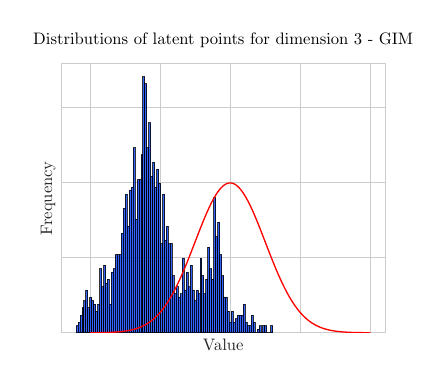
\begin{tikzpicture}[scale=0.6]

\definecolor{blue262255}{RGB}{2,62,255}
\definecolor{darkslategray38}{RGB}{38,38,38}
\definecolor{lightgray204}{RGB}{204,204,204}

\begin{axis}[
axis line style={lightgray204},
tick align=outside,
title={Distributions of latent points for dimension 3 - GIM},
x grid style={lightgray204},
xlabel=\textcolor{darkslategray38}{Value},
xmajorgrids,
xmajorticks=false,
xmin=-4.81721081733704, xmax=4.41986718177795,
xtick style={color=darkslategray38},
y grid style={lightgray204},
ylabel=\textcolor{darkslategray38}{Frequency},
ymajorgrids,
ymajorticks=false,
ymin=0, ymax=0.716212336354062,
ytick style={color=darkslategray38}
]
\draw[draw=black,fill=blue262255,opacity=0.8,line width=0.48pt] (axis cs:-4.39734363555908,0) rectangle (axis cs:-4.34122705459595,0.018947416305663);
\draw[draw=black,fill=blue262255,opacity=0.8,line width=0.48pt] (axis cs:-4.34122657775879,0) rectangle (axis cs:-4.28510999679565,0.0284211244584945);
\draw[draw=black,fill=blue262255,opacity=0.8,line width=0.48pt] (axis cs:-4.28511047363281,0) rectangle (axis cs:-4.22899389266968,0.0473685407641575);
\draw[draw=black,fill=blue262255,opacity=0.8,line width=0.48pt] (axis cs:-4.22899341583252,0) rectangle (axis cs:-4.17287683486938,0.0663159570698205);
\draw[draw=black,fill=blue262255,opacity=0.8,line width=0.48pt] (axis cs:-4.17287731170654,0) rectangle (axis cs:-4.11676073074341,0.0852633733754835);
\draw[draw=black,fill=blue262255,opacity=0.8,line width=0.48pt] (axis cs:-4.11676025390625,0) rectangle (axis cs:-4.06064367294312,0.113684497833978);
\draw[draw=black,fill=blue262255,opacity=0.8,line width=0.48pt] (axis cs:-4.06064414978027,0) rectangle (axis cs:-4.00452756881714,0.0663159570698205);
\draw[draw=black,fill=blue262255,opacity=0.8,line width=0.48pt] (axis cs:-4.00452756881714,0) rectangle (axis cs:-3.94841051101685,0.0947366790272358);
\draw[draw=black,fill=blue262255,opacity=0.8,line width=0.48pt] (axis cs:-3.94841074943542,0) rectangle (axis cs:-3.89229416847229,0.0852633733754835);
\draw[draw=black,fill=blue262255,opacity=0.8,line width=0.48pt] (axis cs:-3.89229416847229,0) rectangle (axis cs:-3.83617758750916,0.075789665222652);
\draw[draw=black,fill=blue262255,opacity=0.8,line width=0.48pt] (axis cs:-3.83617758750916,0) rectangle (axis cs:-3.78006100654602,0.056842248916989);
\draw[draw=black,fill=blue262255,opacity=0.8,line width=0.48pt] (axis cs:-3.78006100654602,0) rectangle (axis cs:-3.72394442558289,0.075789665222652);
\draw[draw=black,fill=blue262255,opacity=0.8,line width=0.48pt] (axis cs:-3.72394442558289,0) rectangle (axis cs:-3.66782784461975,0.170526746750967);
\draw[draw=black,fill=blue262255,opacity=0.8,line width=0.48pt] (axis cs:-3.66782784461975,0) rectangle (axis cs:-3.61171126365662,0.12315820598681);
\draw[draw=black,fill=blue262255,opacity=0.8,line width=0.48pt] (axis cs:-3.61171126365662,0) rectangle (axis cs:-3.55559468269348,0.180000454903799);
\draw[draw=black,fill=blue262255,opacity=0.8,line width=0.48pt] (axis cs:-3.55559468269348,0) rectangle (axis cs:-3.49947810173035,0.132631914139641);
\draw[draw=black,fill=blue262255,opacity=0.8,line width=0.48pt] (axis cs:-3.49947810173035,0) rectangle (axis cs:-3.44336152076721,0.142105622292473);
\draw[draw=black,fill=blue262255,opacity=0.8,line width=0.48pt] (axis cs:-3.44336152076721,0) rectangle (axis cs:-3.38724493980408,0.075789665222652);
\draw[draw=black,fill=blue262255,opacity=0.8,line width=0.48pt] (axis cs:-3.38724493980408,0) rectangle (axis cs:-3.33112835884094,0.161053038598136);
\draw[draw=black,fill=blue262255,opacity=0.8,line width=0.48pt] (axis cs:-3.33112835884094,0) rectangle (axis cs:-3.27501177787781,0.170526746750967);
\draw[draw=black,fill=blue262255,opacity=0.8,line width=0.48pt] (axis cs:-3.27501177787781,0) rectangle (axis cs:-3.21889519691467,0.208421579362293);
\draw[draw=black,fill=blue262255,opacity=0.8,line width=0.48pt] (axis cs:-3.21889543533325,0) rectangle (axis cs:-3.16277837753296,0.208420693859919);
\draw[draw=black,fill=blue262255,opacity=0.8,line width=0.48pt] (axis cs:-3.16277837753296,0) rectangle (axis cs:-3.10666179656982,0.208421579362293);
\draw[draw=black,fill=blue262255,opacity=0.8,line width=0.48pt] (axis cs:-3.10666179656982,0) rectangle (axis cs:-3.05054521560669,0.265263828279282);
\draw[draw=black,fill=blue262255,opacity=0.8,line width=0.48pt] (axis cs:-3.05054521560669,0) rectangle (axis cs:-2.99442863464355,0.331579785349103);
\draw[draw=black,fill=blue262255,opacity=0.8,line width=0.48pt] (axis cs:-2.99442863464355,0) rectangle (axis cs:-2.93831205368042,0.369474617960429);
\draw[draw=black,fill=blue262255,opacity=0.8,line width=0.48pt] (axis cs:-2.93831205368042,0) rectangle (axis cs:-2.88219547271729,0.284211244584945);
\draw[draw=black,fill=blue262255,opacity=0.8,line width=0.48pt] (axis cs:-2.88219547271729,0) rectangle (axis cs:-2.82607889175415,0.37894832611326);
\draw[draw=black,fill=blue262255,opacity=0.8,line width=0.48pt] (axis cs:-2.82607889175415,0) rectangle (axis cs:-2.76996231079102,0.388422034266092);
\draw[draw=black,fill=blue262255,opacity=0.8,line width=0.48pt] (axis cs:-2.76996231079102,0) rectangle (axis cs:-2.71384572982788,0.492632823947238);
\draw[draw=black,fill=blue262255,opacity=0.8,line width=0.48pt] (axis cs:-2.71384572982788,0) rectangle (axis cs:-2.65772914886475,0.303158660890608);
\draw[draw=black,fill=blue262255,opacity=0.8,line width=0.48pt] (axis cs:-2.65772914886475,0) rectangle (axis cs:-2.60161256790161,0.407369450571755);
\draw[draw=black,fill=blue262255,opacity=0.8,line width=0.48pt] (axis cs:-2.60161256790161,0) rectangle (axis cs:-2.54549598693848,0.407369450571755);
\draw[draw=black,fill=blue262255,opacity=0.8,line width=0.48pt] (axis cs:-2.54549598693848,0) rectangle (axis cs:-2.48937940597534,0.473685407641575);
\draw[draw=black,fill=blue262255,opacity=0.8,line width=0.48pt] (axis cs:-2.48937940597534,0) rectangle (axis cs:-2.43326282501221,0.682106987003868);
\draw[draw=black,fill=blue262255,opacity=0.8,line width=0.48pt] (axis cs:-2.43326282501221,0) rectangle (axis cs:-2.37714576721191,0.66315675319065);
\draw[draw=black,fill=blue262255,opacity=0.8,line width=0.48pt] (axis cs:-2.37714600563049,0) rectangle (axis cs:-2.32102942466736,0.492632823947238);
\draw[draw=black,fill=blue262255,opacity=0.8,line width=0.48pt] (axis cs:-2.32102942466736,0) rectangle (axis cs:-2.26491284370422,0.558948781017059);
\draw[draw=black,fill=blue262255,opacity=0.8,line width=0.48pt] (axis cs:-2.26491284370422,0) rectangle (axis cs:-2.20879626274109,0.416843158724586);
\draw[draw=black,fill=blue262255,opacity=0.8,line width=0.48pt] (axis cs:-2.20879626274109,0) rectangle (axis cs:-2.15267968177795,0.454737991335912);
\draw[draw=black,fill=blue262255,opacity=0.8,line width=0.48pt] (axis cs:-2.15267968177795,0) rectangle (axis cs:-2.09656310081482,0.388422034266092);
\draw[draw=black,fill=blue262255,opacity=0.8,line width=0.48pt] (axis cs:-2.09656310081482,0) rectangle (axis cs:-2.04044651985168,0.435790575030249);
\draw[draw=black,fill=blue262255,opacity=0.8,line width=0.48pt] (axis cs:-2.04044651985168,0) rectangle (axis cs:-1.98432993888855,0.397895742418923);
\draw[draw=black,fill=blue262255,opacity=0.8,line width=0.48pt] (axis cs:-1.98432993888855,0) rectangle (axis cs:-1.92821335792542,0.236842703820788);
\draw[draw=black,fill=blue262255,opacity=0.8,line width=0.48pt] (axis cs:-1.92821335792542,0) rectangle (axis cs:-1.87209677696228,0.369474617960429);
\draw[draw=black,fill=blue262255,opacity=0.8,line width=0.48pt] (axis cs:-1.87209677696228,0) rectangle (axis cs:-1.81598019599915,0.246316411973619);
\draw[draw=black,fill=blue262255,opacity=0.8,line width=0.48pt] (axis cs:-1.81598019599915,0) rectangle (axis cs:-1.75986361503601,0.284210640832044);
\draw[draw=black,fill=blue262255,opacity=0.8,line width=0.48pt] (axis cs:-1.75986349582672,0) rectangle (axis cs:-1.70374691486359,0.236842703820788);
\draw[draw=black,fill=blue262255,opacity=0.8,line width=0.48pt] (axis cs:-1.70374691486359,0) rectangle (axis cs:-1.64763033390045,0.236842703820788);
\draw[draw=black,fill=blue262255,opacity=0.8,line width=0.48pt] (axis cs:-1.64763033390045,0) rectangle (axis cs:-1.59151375293732,0.151579330445304);
\draw[draw=black,fill=blue262255,opacity=0.8,line width=0.48pt] (axis cs:-1.59151375293732,0) rectangle (axis cs:-1.53539717197418,0.104210789681147);
\draw[draw=black,fill=blue262255,opacity=0.8,line width=0.48pt] (axis cs:-1.53539717197418,0) rectangle (axis cs:-1.47928059101105,0.12315820598681);
\draw[draw=black,fill=blue262255,opacity=0.8,line width=0.48pt] (axis cs:-1.47928059101105,0) rectangle (axis cs:-1.42316401004791,0.094737081528315);
\draw[draw=black,fill=blue262255,opacity=0.8,line width=0.48pt] (axis cs:-1.42316389083862,0) rectangle (axis cs:-1.36704730987549,0.104210568305083);
\draw[draw=black,fill=blue262255,opacity=0.8,line width=0.48pt] (axis cs:-1.36704730987549,0) rectangle (axis cs:-1.31093072891235,0.198947871209462);
\draw[draw=black,fill=blue262255,opacity=0.8,line width=0.48pt] (axis cs:-1.31093072891235,0) rectangle (axis cs:-1.25481414794922,0.113684497833978);
\draw[draw=black,fill=blue262255,opacity=0.8,line width=0.48pt] (axis cs:-1.25481414794922,0) rectangle (axis cs:-1.19869756698608,0.161053038598136);
\draw[draw=black,fill=blue262255,opacity=0.8,line width=0.48pt] (axis cs:-1.19869756698608,0) rectangle (axis cs:-1.14258098602295,0.12315820598681);
\draw[draw=black,fill=blue262255,opacity=0.8,line width=0.48pt] (axis cs:-1.14258098602295,0) rectangle (axis cs:-1.08646440505981,0.180000454903799);
\draw[draw=black,fill=blue262255,opacity=0.8,line width=0.48pt] (axis cs:-1.08646440505981,0) rectangle (axis cs:-1.03034782409668,0.113684497833978);
\draw[draw=black,fill=blue262255,opacity=0.8,line width=0.48pt] (axis cs:-1.03034782409668,0) rectangle (axis cs:-0.974231243133545,0.0852632828124521);
\draw[draw=black,fill=blue262255,opacity=0.8,line width=0.48pt] (axis cs:-0.9742311835289,0) rectangle (axis cs:-0.918114602565765,0.113684497833978);
\draw[draw=black,fill=blue262255,opacity=0.8,line width=0.48pt] (axis cs:-0.918114542961121,0) rectangle (axis cs:-0.861997961997986,0.104210678992997);
\draw[draw=black,fill=blue262255,opacity=0.8,line width=0.48pt] (axis cs:-0.861997961997986,0) rectangle (axis cs:-0.805881381034851,0.198947871209462);
\draw[draw=black,fill=blue262255,opacity=0.8,line width=0.48pt] (axis cs:-0.805881381034851,0) rectangle (axis cs:-0.749764800071716,0.151579330445304);
\draw[draw=black,fill=blue262255,opacity=0.8,line width=0.48pt] (axis cs:-0.749764800071716,0) rectangle (axis cs:-0.693648219108582,0.104210789681147);
\draw[draw=black,fill=blue262255,opacity=0.8,line width=0.48pt] (axis cs:-0.693648219108582,0) rectangle (axis cs:-0.637531638145447,0.142105471354087);
\draw[draw=black,fill=blue262255,opacity=0.8,line width=0.48pt] (axis cs:-0.637531578540802,0) rectangle (axis cs:-0.581414997577667,0.227368995667956);
\draw[draw=black,fill=blue262255,opacity=0.8,line width=0.48pt] (axis cs:-0.581414997577667,0) rectangle (axis cs:-0.525298416614532,0.170526746750967);
\draw[draw=black,fill=blue262255,opacity=0.8,line width=0.48pt] (axis cs:-0.525298416614532,0) rectangle (axis cs:-0.469181835651398,0.14210554682324);
\draw[draw=black,fill=blue262255,opacity=0.8,line width=0.48pt] (axis cs:-0.469181776046753,0) rectangle (axis cs:-0.413065195083618,0.360000718618874);
\draw[draw=black,fill=blue262255,opacity=0.8,line width=0.48pt] (axis cs:-0.413065195083618,0) rectangle (axis cs:-0.356948614120483,0.255790120126451);
\draw[draw=black,fill=blue262255,opacity=0.8,line width=0.48pt] (axis cs:-0.356948614120483,0) rectangle (axis cs:-0.300832033157349,0.293684796768029);
\draw[draw=black,fill=blue262255,opacity=0.8,line width=0.48pt] (axis cs:-0.300832003355026,0) rectangle (axis cs:-0.244715422391891,0.208421524018174);
\draw[draw=black,fill=blue262255,opacity=0.8,line width=0.48pt] (axis cs:-0.244715392589569,0) rectangle (axis cs:-0.188598811626434,0.151579290195036);
\draw[draw=black,fill=blue262255,opacity=0.8,line width=0.48pt] (axis cs:-0.188598811626434,0) rectangle (axis cs:-0.1324822306633,0.0947370563718974);
\draw[draw=black,fill=blue262255,opacity=0.8,line width=0.48pt] (axis cs:-0.132482200860977,0) rectangle (axis cs:-0.0763656198978424,0.0947370563718974);
\draw[draw=black,fill=blue262255,opacity=0.8,line width=0.48pt] (axis cs:-0.0763656049966812,0) rectangle (axis cs:-0.0202490240335464,0.0568422262762161);
\draw[draw=black,fill=blue262255,opacity=0.8,line width=0.48pt] (axis cs:-0.0202490109950304,0) rectangle (axis cs:0.0358675718307495,0.0284211169115692);
\draw[draw=black,fill=blue262255,opacity=0.8,line width=0.48pt] (axis cs:0.0358675867319107,0) rectangle (axis cs:0.0919841676950455,0.0568422338231384);
\draw[draw=black,fill=blue262255,opacity=0.8,line width=0.48pt] (axis cs:0.0919841825962067,0) rectangle (axis cs:0.148100763559341,0.0284211131381081);
\draw[draw=black,fill=blue262255,opacity=0.8,line width=0.48pt] (axis cs:0.148100793361664,0) rectangle (axis cs:0.204217374324799,0.037894822548759);
\draw[draw=black,fill=blue262255,opacity=0.8,line width=0.48pt] (axis cs:0.204217374324799,0) rectangle (axis cs:0.260333955287933,0.0473685407641575);
\draw[draw=black,fill=blue262255,opacity=0.8,line width=0.48pt] (axis cs:0.260333955287933,0) rectangle (axis cs:0.316450536251068,0.0473685156077465);
\draw[draw=black,fill=blue262255,opacity=0.8,line width=0.48pt] (axis cs:0.316450595855713,0) rectangle (axis cs:0.372567176818848,0.0473685156077465);
\draw[draw=black,fill=blue262255,opacity=0.8,line width=0.48pt] (axis cs:0.372567176818848,0) rectangle (axis cs:0.428683757781982,0.075789665222652);
\draw[draw=black,fill=blue262255,opacity=0.8,line width=0.48pt] (axis cs:0.428683757781982,0) rectangle (axis cs:0.484800338745117,0.0284211093646479);
\draw[draw=black,fill=blue262255,opacity=0.8,line width=0.48pt] (axis cs:0.484800398349762,0) rectangle (axis cs:0.540916979312897,0.0189474062430986);
\draw[draw=black,fill=blue262255,opacity=0.8,line width=0.48pt] (axis cs:0.540916979312897,0) rectangle (axis cs:0.597033560276031,0.018947416305663);
\draw[draw=black,fill=blue262255,opacity=0.8,line width=0.48pt] (axis cs:0.597033560276031,0) rectangle (axis cs:0.653150141239166,0.0473685407641575);
\draw[draw=black,fill=blue262255,opacity=0.8,line width=0.48pt] (axis cs:0.653150141239166,0) rectangle (axis cs:0.709266722202301,0.0284211244584945);
\draw[draw=black,fill=blue262255,opacity=0.8,line width=0.48pt] (axis cs:0.709266781806946,0) rectangle (axis cs:0.765383362770081,0);
\draw[draw=black,fill=blue262255,opacity=0.8,line width=0.48pt] (axis cs:0.765383362770081,0) rectangle (axis cs:0.821499943733215,0.00947370815283151);
\draw[draw=black,fill=blue262255,opacity=0.8,line width=0.48pt] (axis cs:0.821499943733215,0) rectangle (axis cs:0.87761652469635,0.018947416305663);
\draw[draw=black,fill=blue262255,opacity=0.8,line width=0.48pt] (axis cs:0.87761652469635,0) rectangle (axis cs:0.933733105659485,0);
\draw[draw=black,fill=blue262255,opacity=0.8,line width=0.48pt] (axis cs:0.93373316526413,0) rectangle (axis cs:0.989849746227264,0.018947416305663);
\draw[draw=black,fill=blue262255,opacity=0.8,line width=0.48pt] (axis cs:0.989849805831909,0) rectangle (axis cs:1.04596638679504,0.0189473961805449);
\draw[draw=black,fill=blue262255,opacity=0.8,line width=0.48pt] (axis cs:1.04596638679504,0) rectangle (axis cs:1.10208296775818,0);
\draw[draw=black,fill=blue262255,opacity=0.8,line width=0.48pt] (axis cs:1.10208296775818,0) rectangle (axis cs:1.15819954872131,0);
\draw[draw=black,fill=blue262255,opacity=0.8,line width=0.48pt] (axis cs:1.15819954872131,0) rectangle (axis cs:1.21431612968445,0.018947416305663);
\addplot [thick, red]
table {%
-4 0.000133830225764885
-3.99199199199199 0.000138182046410498
-3.98398398398398 0.000142666228042307
-3.97597597597598 0.000147286481503254
-3.96796796796797 0.000152046611333821
-3.95995995995996 0.000156950517814782
-3.95195195195195 0.00016200219904485
-3.94394394394394 0.00016720575305353
-3.93593593593594 0.000172565379949496
-3.92792792792793 0.00017808538410479
-3.91991991991992 0.000183770176375138
-3.91191191191191 0.000189624276356684
-3.9039039039039 0.000195652314679408
-3.8958958958959 0.000201859035337517
-3.88788788788789 0.000208249298057069
-3.87987987987988 0.000214828080701088
-3.87187187187187 0.000221600481712426
-3.86386386386386 0.0002285717225946
-3.85585585585586 0.000235747150430845
-3.84784784784785 0.000243132240441603
-3.83983983983984 0.000250732598580649
-3.83183183183183 0.000258553964170059
-3.82382382382382 0.000266602212574213
-3.81581581581582 0.000274883357912987
-3.80780780780781 0.000283403555814325
-3.7997997997998 0.000292169106206322
-3.79179179179179 0.000301186456148957
-3.78378378378378 0.0003104622027056
-3.77577577577578 0.000320003095854415
-3.76776776776777 0.000329816041439723
-3.75975975975976 0.000339908104163431
-3.75175175175175 0.00035028651061658
-3.74374374374374 0.000360958652351047
-3.73573573573574 0.000371932088991451
-3.72772772772773 0.000383214551387261
-3.71971971971972 0.000394813944805093
-3.71171171171171 0.000406738352161197
-3.7037037037037 0.000418996037294058
-3.6956956956957 0.00043159544827708
-3.68768768768769 0.00044454522077123
-3.67967967967968 0.000457854181417586
-3.67167167167167 0.000471531351269624
-3.66366366366366 0.000485585949265103
-3.65565565565566 0.000500027395737409
-3.64764764764765 0.000514865315966112
-3.63963963963964 0.000530109543766577
-3.63163163163163 0.000545770125118336
-3.62362362362362 0.000561857321831991
-3.61561561561562 0.00057838161525435
-3.60760760760761 0.000595353710011453
-3.5995995995996 0.000612784537789192
-3.59159159159159 0.000630685261151105
-3.58358358358358 0.000649067277392973
-3.57557557557558 0.000667942222433796
-3.56756756756757 0.000687321974742665
-3.55955955955956 0.000707218659301081
-3.55155155155155 0.000727644651600166
-3.54354354354354 0.000748612581672245
-3.53553553553554 0.000770135338156225
-3.52752752752753 0.000792226072396121
-3.51951951951952 0.00081489820257214
-3.51151151151151 0.000838165417863603
-3.5035035035035 0.000862041682643007
-3.4954954954955 0.000886541240700502
-3.48748748748749 0.00091167861949796
-3.47947947947948 0.000937468634451866
-3.47147147147147 0.000963926393244149
-3.46346346346346 0.000991067300160059
-3.45545545545546 0.0010189070604522
-3.44744744744745 0.00104746168472971
-3.43943943943944 0.0010767474933716
-3.43143143143143 0.00110678112096323
-3.42342342342342 0.00113757952075483
-3.41541541541542 0.00116915996914087
-3.40740740740741 0.00120154007015926
-3.3993993993994 0.00123473776000907
-3.39139139139139 0.00126877131158549
-3.38338338338338 0.00130365933903088
-3.37537537537538 0.00133942080230046
-3.36736736736737 0.00137607501174126
-3.35935935935936 0.001413641632683
-3.35135135135135 0.00145214069003938
-3.34334334334334 0.0014915925729182
-3.33533533533534 0.00153201803923895
-3.32732732732733 0.00157343822035606
-3.31931931931932 0.00161587462568624
-3.31131131131131 0.00165934914733831
-3.3033033033033 0.00170388406474362
-3.2952952952953 0.00174950204928538
-3.28728728728729 0.00179622616892505
-3.27927927927928 0.00184407989282385
-3.27127127127127 0.00189308709595757
-3.26326326326326 0.00194327206372255
-3.25525525525526 0.00199465949653091
-3.24724724724725 0.00204727451439301
-3.23923923923924 0.00210114266148476
-3.23123123123123 0.00215628991069791
-3.22322322322322 0.00221274266817093
-3.21521521521522 0.00227052777779815
-3.20720720720721 0.00232967252571501
-3.1991991991992 0.00239020464475689
-3.19119119119119 0.00245215231888918
-3.18318318318318 0.00251554418760605
-3.17517517517518 0.00258040935029545
-3.16716716716717 0.00264677737056774
-3.15915915915916 0.00271467828054534
-3.15115115115115 0.00278414258511061
-3.14314314314314 0.00285520126610952
-3.13513513513514 0.00292788578650791
-3.12712712712713 0.00300222809449793
-3.11911911911912 0.00307826062755151
-3.11111111111111 0.00315601631641804
-3.1031031031031 0.00323552858906328
-3.0950950950951 0.00331683137454643
-3.08708708708709 0.00339995910683238
-3.07907907907908 0.00348494672853595
-3.07107107107107 0.00357182969459489
-3.06306306306306 0.00366064397586864
-3.05505505505506 0.00375142606265932
-3.04704704704705 0.00384421296815189
-3.03903903903904 0.00393904223176991
-3.03103103103103 0.00403595192244368
-3.02302302302302 0.0041349806417872
-3.01501501501502 0.00423616752718052
-3.00700700700701 0.00433955225475399
-2.998998998999 0.00444517504227068
-2.99099099099099 0.00455307665190355
-2.98298298298298 0.00466329839290368
-2.97497497497497 0.00477588212415564
-2.96696696696697 0.00489087025661667
-2.95895895895896 0.00500830575563558
-2.95095095095095 0.00512823214314763
-2.94294294294294 0.00525069349974172
-2.93493493493493 0.00537573446659573
-2.92692692692693 0.00550340024727644
-2.91891891891892 0.00563373660939975
-2.91091091091091 0.0057667898861475
-2.9029029029029 0.00590260697763674
-2.89489489489489 0.00604123535213746
-2.88688688688689 0.00618272304713484
-2.87887887887888 0.00632711867023164
-2.87087087087087 0.00647447139988703
-2.86286286286286 0.00662483098598741
-2.85485485485485 0.0067782477502453
-2.84684684684685 0.0069347725864219
-2.83883883883884 0.00709445696036946
-2.83083083083083 0.00725735290988893
-2.82282282282282 0.00742351304439893
-2.81481481481481 0.00759299054441176
-2.80680680680681 0.0077658391608121
-2.7987987987988 0.00794211321393437
-2.79079079079079 0.00812186759243432
-2.78278278278278 0.00830515775195071
-2.77477477477477 0.00849203971355293
-2.76676676676677 0.00868257006197001
-2.75875875875876 0.00887680594359712
-2.75075075075075 0.00907480506427511
-2.74274274274274 0.00927662568683898
-2.73473473473473 0.00948232662843099
-2.72672672672673 0.00969196725757422
-2.71871871871872 0.00990560749100246
-2.71071071071071 0.0101233077902421
-2.7027027027027 0.0103451291579421
-2.69469469469469 0.0105711331339476
-2.68668668668669 0.0108013817911136
-2.67867867867868 0.011035937730854
-2.67067067067067 0.0112748640784219
-2.66266266266266 0.0115182244779185
-2.65465465465465 0.0117660830870247
-2.64664664664665 0.0120185045714526
-2.63863863863864 0.0122755540991133
-2.63063063063063 0.0125372973339956
-2.62262262262262 0.0128038004297541
-2.61461461461461 0.0130751300230007
-2.60660660660661 0.0133513532262973
-2.5985985985986 0.0136325376208454
-2.59059059059059 0.0139187512488692
-2.58258258258258 0.014210062605689
-2.57457457457457 0.0145065406314803
-2.56656656656657 0.0148082547027168
-2.55855855855856 0.0151152746232934
-2.55055055055055 0.0154276706153247
-2.54254254254254 0.0157455133096184
-2.53453453453453 0.0160688737358178
-2.52652652652653 0.016397823312213
-2.51851851851852 0.0167324338352151
-2.51051051051051 0.0170727774684938
-2.5025025025025 0.0174189267317727
-2.49449449449449 0.0177709544892815
-2.48648648648649 0.0181289339378627
-2.47847847847848 0.0184929385947284
-2.47047047047047 0.0188630422848682
-2.46246246246246 0.0192393191281025
-2.45445445445445 0.0196218435257817
-2.44644644644645 0.0200106901471285
-2.43843843843844 0.020405933915221
-2.43043043043043 0.0208076499926159
-2.42242242242242 0.0212159137666093
-2.41441441441441 0.0216308008341344
-2.40640640640641 0.0220523869862944
-2.3983983983984 0.0224807481925294
-2.39039039039039 0.022915960584417
-2.38238238238238 0.0233581004391047
-2.37437437437437 0.023807244162374
-2.36636636636637 0.0242634682713357
-2.35835835835836 0.0247268493767558
-2.35035035035035 0.0251974641650118
-2.34234234234234 0.0256753893796796
-2.33433433433433 0.0261607018027501
-2.32632632632633 0.0266534782354775
-2.31831831831832 0.0271537954788581
-2.31031031031031 0.0276617303137407
-2.3023023023023 0.0281773594805703
-2.29429429429429 0.0287007596587648
-2.28628628628629 0.0292320074457259
-2.27827827827828 0.029771179335487
-2.27027027027027 0.0303183516969979
-2.26226226226226 0.0308736007520491
-2.25425425425425 0.0314370025528369
-2.24624624624625 0.0320086329591723
-2.23823823823824 0.0325885676153351
-2.23023023023023 0.0331768819265761
-2.22222222222222 0.0337736510352706
-2.21421421421421 0.0343789497967251
-2.20620620620621 0.0349928527546413
-2.1981981981982 0.0356154341162401
-2.19019019019019 0.0362467677270497
-2.18218218218218 0.0368869270453615
-2.17417417417417 0.0375359851163567
-2.16616616616617 0.03819401454591
-2.15815815815816 0.0388610874740724
-2.15015015015015 0.03953727554824
-2.14214214214214 0.0402226498960119
-2.13413413413413 0.0409172810977437
-2.12612612612613 0.0416212391588003
-2.11811811811812 0.0423345934815158
-2.11011011011011 0.0430574128368641
-2.1021021021021 0.043789765335848
-2.09409409409409 0.0445317184006117
-2.08608608608609 0.0452833387352837
-2.07807807807808 0.0460446922965577
-2.07007007007007 0.0468158442640166
-2.06206206206206 0.0475968590102091
-2.05405405405405 0.0483878000704834
-2.04604604604605 0.0491887301125894
-2.03803803803804 0.0499997109060533
-2.03003003003003 0.0508208032913361
-2.02202202202202 0.0516520671487823
-2.01401401401401 0.0524935613673682
-2.00600600600601 0.053345343813258
-1.997997997998 0.0542074712981785
-1.98998998998999 0.0550799995476186
-1.98198198198198 0.0559629831688668
-1.97397397397397 0.0568564756188931
-1.96596596596597 0.0577605291720876
-1.95795795795796 0.0586751948878651
-1.94994994994995 0.0596005225781457
-1.94194194194194 0.0605365607747232
-1.93393393393393 0.0614833566965309
-1.92592592592593 0.062440956216817
-1.91791791791792 0.06340940383024
-1.90990990990991 0.0643887426198963
-1.9019019019019 0.0653790142242912
-1.89389389389389 0.0663802588042656
-1.88588588588589 0.0673925150098903
-1.87787787787788 0.0684158199473405
-1.86986986986987 0.0694502091457625
-1.86186186186186 0.0704957165241465
-1.85385385385385 0.0715523743582165
-1.84584584584585 0.0726202132473521
-1.83783783783784 0.0736992620815557
-1.82982982982983 0.0747895480084762
-1.82182182182182 0.0758910964005057
-1.81381381381381 0.0770039308219614
-1.80580580580581 0.0781280729963669
-1.7977977977978 0.0792635427738473
-1.78978978978979 0.0804103580986525
-1.78178178178178 0.0815685349768227
-1.77377377377377 0.0827380874440109
-1.76576576576577 0.0839190275334777
-1.75775775775776 0.0851113652442723
-1.74974974974975 0.086315108509615
-1.74174174174174 0.0875302631654975
-1.73373373373373 0.0887568329195139
-1.72572572572573 0.0899948193199405
-1.71771771771772 0.0912442217250772
-1.70970970970971 0.0925050372728685
-1.7017017017017 0.0937772608508177
-1.69369369369369 0.0950608850662112
-1.68568568568569 0.0963559002166691
-1.67767767767768 0.0976622942610365
-1.66966966966967 0.0989800527906321
-1.66166166166166 0.100309159000872
-1.65365365365365 0.10164959366328
-1.64564564564565 0.103001335097907
-1.63763763763764 0.10436435914617
-1.62962962962963 0.105738639144131
-1.62162162162162 0.107124145896225
-1.61361361361361 0.108520847649465
-1.60560560560561 0.10992871006813
-1.5975975975976 0.111347696208955
-1.58958958958959 0.112777766496842
-1.58158158158158 0.114218878701105
-1.57357357357357 0.115670987912262
-1.56556556556557 0.117134046519405
-1.55755755755756 0.11860800418814
-1.54954954954955 0.120092807839133
-1.54154154154154 0.121588401627275
-1.53353353353353 0.123094726921466
-1.52552552552553 0.124611722285057
-1.51751751751752 0.12613932345695
-1.50950950950951 0.127677463333369
-1.5015015015015 0.129226071950339
-1.49349349349349 0.130785076466857
-1.48548548548549 0.132354401148798
-1.47747747747748 0.133933967353555
-1.46946946946947 0.13552369351543
-1.46146146146146 0.137123495131801
-1.45345345345345 0.13873328475006
-1.44544544544545 0.140352971955359
-1.43743743743744 0.141982463359159
-1.42942942942943 0.143621662588612
-1.42142142142142 0.14527047027677
-1.41341341341341 0.146928784053658
-1.40540540540541 0.148596498538208
-1.3973973973974 0.150273505331067
-1.38938938938939 0.151959693008306
-1.38138138138138 0.153654947116025
-1.37337337337337 0.155359150165875
-1.36536536536537 0.157072181631514
-1.35735735735736 0.158793917945997
-1.34934934934935 0.160524232500121
-1.34134134134134 0.16226299564173
-1.33333333333333 0.164010074675994
-1.32532532532533 0.165765333866673
-1.31731731731732 0.167528634438376
-1.30930930930931 0.169299834579821
-1.3013013013013 0.17107878944811
-1.29329329329329 0.172865351174024
-1.28528528528529 0.174659368868355
-1.27727727727728 0.176460688629273
-1.26926926926927 0.178269153550739
-1.26126126126126 0.180084603731981
-1.25325325325325 0.181906876288021
-1.24524524524525 0.183735805361283
-1.23723723723724 0.185571222134271
-1.22922922922923 0.187412954843324
-1.22122122122122 0.18926082879347
-1.21321321321321 0.191114666374361
-1.20520520520521 0.192974287077311
-1.1971971971972 0.194839507513435
-1.18918918918919 0.19671014143289
-1.18118118118118 0.198585999745227
-1.17317317317317 0.200466890540856
-1.16516516516517 0.202352619113618
-1.15715715715716 0.204242987984477
-1.14914914914915 0.206137796926331
-1.14114114114114 0.208036842989938
-1.13313313313313 0.209939920530956
-1.12512512512513 0.21184682123811
-1.11711711711712 0.21375733416247
-1.10910910910911 0.215671245747847
-1.1011011011011 0.217588339862305
-1.09309309309309 0.219508397830784
-1.08508508508509 0.221431198468836
-1.07707707707708 0.223356518117463
-1.06906906906907 0.225284130679063
-1.06106106106106 0.22721380765447
-1.05305305305305 0.229145318181096
-1.04504504504505 0.231078429072154
-1.03703703703704 0.233012904856966
-1.02902902902903 0.234948507822352
-1.02102102102102 0.236884998055083
-1.01301301301301 0.238822133485401
-1.00500500500501 0.24075966993159
-0.996996996996997 0.242697361145593
-0.988988988988989 0.244634958859672
-0.980980980980981 0.246572212834085
-0.972972972972973 0.248508870905785
-0.964964964964965 0.250444679038131
-0.956956956956957 0.252379381371581
-0.948948948948949 0.254312720275385
-0.940940940940941 0.256244436400228
-0.932932932932933 0.258174268731856
-0.924924924924925 0.260101954645624
-0.916916916916917 0.262027229961987
-0.908908908908909 0.263949829002911
-0.900900900900901 0.265869484649172
-0.892892892892893 0.267785928398552
-0.884884884884885 0.269698890424904
-0.876876876876877 0.271608099638066
-0.868868868868869 0.273513283744617
-0.860860860860861 0.275414169309444
-0.852852852852853 0.277310481818125
-0.844844844844845 0.279201945740075
-0.836836836836837 0.281088284592474
-0.828828828828829 0.28296922100493
-0.820820820820821 0.284844476784867
-0.812812812812813 0.286713772983616
-0.804804804804805 0.288576829963198
-0.796796796796797 0.290433367463758
-0.788788788788789 0.292283104671645
-0.780780780780781 0.294125760288111
-0.772772772772773 0.295961052598604
-0.764764764764765 0.29778869954263
-0.756756756756757 0.299608418784177
-0.748748748748749 0.301419927782648
-0.740740740740741 0.303222943864308
-0.732732732732733 0.305017184294205
-0.724724724724725 0.306802366348536
-0.716716716716717 0.308578207387456
-0.708708708708709 0.310344424928268
-0.700700700700701 0.312100736719007
-0.692692692692693 0.313846860812361
-0.684684684684685 0.31558251563992
-0.676676676676677 0.317307420086723
-0.668668668668669 0.319021293566066
-0.660660660660661 0.320723856094559
-0.652652652652653 0.322414828367396
-0.644644644644645 0.324093931833804
-0.636636636636636 0.325760888772662
-0.628628628628629 0.327415422368237
-0.620620620620621 0.329057256786028
-0.612612612612613 0.330686117248681
-0.604604604604605 0.33230173011195
-0.596596596596596 0.333903822940662
-0.588588588588589 0.335492124584683
-0.580580580580581 0.337066365254824
-0.572572572572573 0.338626276598684
-0.564564564564565 0.340171591776383
-0.556556556556556 0.341702045536168
-0.548548548548549 0.343217374289848
-0.54054054054054 0.344717316188045
-0.532532532532533 0.346201611195215
-0.524524524524525 0.347670001164422
-0.516516516516516 0.349122229911825
-0.508508508508509 0.350558043290856
-0.5005005005005 0.351977189266054
-0.492492492492492 0.353379417986526
-0.484484484484485 0.354764481859011
-0.476476476476476 0.356132135620502
-0.468468468468469 0.357482136410418
-0.46046046046046 0.358814243842273
-0.452452452452452 0.360128220074839
-0.444444444444445 0.361423829882744
-0.436436436436436 0.362700840726495
-0.428428428428429 0.363959022821904
-0.42042042042042 0.365198149208855
-0.412412412412412 0.366417995819425
-0.404404404404405 0.3676183415453
-0.396396396396396 0.368798968304465
-0.388388388388389 0.369959661107154
-0.38038038038038 0.37110020812101
-0.372372372372372 0.372220400735444
-0.364364364364365 0.373320033625156
-0.356356356356356 0.374398904812801
-0.348348348348348 0.375456815730761
-0.34034034034034 0.376493571282005
-0.332332332332332 0.377508979900006
-0.324324324324325 0.378502853607702
-0.316316316316316 0.379475008075448
-0.308308308308308 0.380425262677969
-0.3003003003003 0.38135344055026
-0.292292292292292 0.382259368642425
-0.284284284284285 0.38314287777343
-0.276276276276276 0.384003802683735
-0.268268268268268 0.3848419820868
-0.26026026026026 0.385657258719425
-0.252252252252252 0.386449479390916
-0.244244244244244 0.387218495031049
-0.236236236236236 0.387964160736805
-0.228228228228228 0.38868633581787
-0.22022022022022 0.389384883840873
-0.212212212212212 0.390059672672329
-0.204204204204204 0.390710574520297
-0.196196196196196 0.391337465974705
-0.188188188188188 0.39194022804635
-0.18018018018018 0.392518746204527
-0.172172172172172 0.393072910413305
-0.164164164164164 0.393602615166401
-0.156156156156156 0.394107759520658
-0.148148148148148 0.394588247128102
-0.14014014014014 0.395043986266573
-0.132132132132132 0.3954748898689
-0.124124124124124 0.395880875550626
-0.116116116116116 0.396261865636259
-0.108108108108108 0.396617787184037
-0.1001001001001 0.396948572009207
-0.0920920920920922 0.397254156705792
-0.084084084084084 0.397534482666846
-0.0760760760760761 0.39778949610319
-0.0680680680680683 0.39801914806061
-0.06006006006006 0.398223394435522
-0.0520520520520522 0.398402195989086
-0.0440440440440439 0.398555518359772
-0.0360360360360361 0.398683332074364
-0.0280280280280278 0.398785612557403
-0.02002002002002 0.398862340139061
-0.0120120120120122 0.398913500061449
-0.00400400400400391 0.398939082483343
0.00400400400400436 0.398939082483343
0.0120120120120122 0.398913500061449
0.02002002002002 0.398862340139061
0.0280280280280278 0.398785612557403
0.0360360360360357 0.398683332074364
0.0440440440440444 0.398555518359772
0.0520520520520522 0.398402195989086
0.06006006006006 0.398223394435522
0.0680680680680679 0.39801914806061
0.0760760760760757 0.39778949610319
0.0840840840840844 0.397534482666846
0.0920920920920922 0.397254156705792
0.1001001001001 0.396948572009207
0.108108108108108 0.396617787184037
0.116116116116116 0.396261865636259
0.124124124124124 0.395880875550626
0.132132132132132 0.3954748898689
0.14014014014014 0.395043986266573
0.148148148148148 0.394588247128102
0.156156156156156 0.394107759520658
0.164164164164164 0.393602615166401
0.172172172172172 0.393072910413305
0.18018018018018 0.392518746204527
0.188188188188188 0.39194022804635
0.196196196196196 0.391337465974705
0.204204204204204 0.390710574520297
0.212212212212212 0.390059672672329
0.22022022022022 0.389384883840873
0.228228228228228 0.388686335817871
0.236236236236236 0.387964160736805
0.244244244244245 0.387218495031049
0.252252252252252 0.386449479390916
0.26026026026026 0.385657258719425
0.268268268268268 0.3848419820868
0.276276276276276 0.384003802683735
0.284284284284285 0.38314287777343
0.292292292292292 0.382259368642425
0.3003003003003 0.38135344055026
0.308308308308308 0.380425262677969
0.316316316316316 0.379475008075448
0.324324324324325 0.378502853607702
0.332332332332332 0.377508979900006
0.34034034034034 0.376493571282005
0.348348348348348 0.375456815730762
0.356356356356356 0.374398904812801
0.364364364364365 0.373320033625156
0.372372372372372 0.372220400735444
0.38038038038038 0.37110020812101
0.388388388388388 0.369959661107154
0.396396396396397 0.368798968304465
0.404404404404405 0.3676183415453
0.412412412412412 0.366417995819425
0.42042042042042 0.365198149208855
0.428428428428428 0.363959022821904
0.436436436436437 0.362700840726495
0.444444444444445 0.361423829882744
0.452452452452452 0.360128220074839
0.46046046046046 0.358814243842273
0.468468468468468 0.357482136410418
0.476476476476477 0.356132135620502
0.484484484484485 0.354764481859011
0.492492492492492 0.353379417986526
0.5005005005005 0.351977189266054
0.508508508508508 0.350558043290856
0.516516516516517 0.349122229911825
0.524524524524525 0.347670001164422
0.532532532532533 0.346201611195215
0.54054054054054 0.344717316188045
0.548548548548548 0.343217374289848
0.556556556556557 0.341702045536168
0.564564564564565 0.340171591776383
0.572572572572573 0.338626276598684
0.58058058058058 0.337066365254824
0.588588588588588 0.335492124584683
0.596596596596597 0.333903822940662
0.604604604604605 0.33230173011195
0.612612612612613 0.330686117248681
0.62062062062062 0.329057256786028
0.628628628628628 0.327415422368237
0.636636636636637 0.325760888772662
0.644644644644645 0.324093931833804
0.652652652652653 0.322414828367396
0.66066066066066 0.32072385609456
0.668668668668668 0.319021293566066
0.676676676676677 0.317307420086723
0.684684684684685 0.31558251563992
0.692692692692693 0.313846860812361
0.7007007007007 0.312100736719007
0.708708708708708 0.310344424928268
0.716716716716717 0.308578207387456
0.724724724724725 0.306802366348536
0.732732732732733 0.305017184294205
0.74074074074074 0.303222943864308
0.748748748748748 0.301419927782648
0.756756756756757 0.299608418784177
0.764764764764765 0.29778869954263
0.772772772772773 0.295961052598604
0.780780780780781 0.294125760288111
0.788788788788788 0.292283104671645
0.796796796796797 0.290433367463758
0.804804804804805 0.288576829963198
0.812812812812813 0.286713772983616
0.820820820820821 0.284844476784867
0.828828828828828 0.282969221004931
0.836836836836837 0.281088284592474
0.844844844844845 0.279201945740075
0.852852852852853 0.277310481818125
0.860860860860861 0.275414169309444
0.868868868868869 0.273513283744617
0.876876876876877 0.271608099638066
0.884884884884885 0.269698890424904
0.892892892892893 0.267785928398552
0.900900900900901 0.265869484649172
0.908908908908909 0.263949829002911
0.916916916916917 0.262027229961987
0.924924924924925 0.260101954645624
0.932932932932933 0.258174268731856
0.940940940940941 0.256244436400228
0.948948948948949 0.254312720275384
0.956956956956957 0.252379381371581
0.964964964964965 0.250444679038131
0.972972972972973 0.248508870905785
0.980980980980981 0.246572212834085
0.988988988988989 0.244634958859672
0.996996996996997 0.242697361145593
1.00500500500501 0.24075966993159
1.01301301301301 0.238822133485401
1.02102102102102 0.236884998055083
1.02902902902903 0.234948507822352
1.03703703703704 0.233012904856966
1.04504504504505 0.231078429072154
1.05305305305305 0.229145318181096
1.06106106106106 0.22721380765447
1.06906906906907 0.225284130679062
1.07707707707708 0.223356518117463
1.08508508508509 0.221431198468836
1.09309309309309 0.219508397830784
1.1011011011011 0.217588339862305
1.10910910910911 0.215671245747847
1.11711711711712 0.21375733416247
1.12512512512513 0.21184682123811
1.13313313313313 0.209939920530956
1.14114114114114 0.208036842989938
1.14914914914915 0.206137796926331
1.15715715715716 0.204242987984477
1.16516516516517 0.202352619113618
1.17317317317317 0.200466890540856
1.18118118118118 0.198585999745228
1.18918918918919 0.19671014143289
1.1971971971972 0.194839507513435
1.20520520520521 0.192974287077311
1.21321321321321 0.191114666374361
1.22122122122122 0.18926082879347
1.22922922922923 0.187412954843324
1.23723723723724 0.185571222134271
1.24524524524525 0.183735805361283
1.25325325325325 0.181906876288021
1.26126126126126 0.180084603731981
1.26926926926927 0.178269153550739
1.27727727727728 0.176460688629273
1.28528528528529 0.174659368868355
1.29329329329329 0.172865351174024
1.3013013013013 0.17107878944811
1.30930930930931 0.169299834579821
1.31731731731732 0.167528634438376
1.32532532532533 0.165765333866673
1.33333333333333 0.164010074675994
1.34134134134134 0.16226299564173
1.34934934934935 0.160524232500121
1.35735735735736 0.158793917945997
1.36536536536537 0.157072181631514
1.37337337337337 0.155359150165875
1.38138138138138 0.153654947116025
1.38938938938939 0.151959693008306
1.3973973973974 0.150273505331067
1.40540540540541 0.148596498538208
1.41341341341341 0.146928784053658
1.42142142142142 0.14527047027677
1.42942942942943 0.143621662588612
1.43743743743744 0.141982463359159
1.44544544544545 0.140352971955359
1.45345345345345 0.13873328475006
1.46146146146146 0.137123495131801
1.46946946946947 0.13552369351543
1.47747747747748 0.133933967353555
1.48548548548549 0.132354401148798
1.49349349349349 0.130785076466857
1.5015015015015 0.129226071950339
1.50950950950951 0.127677463333369
1.51751751751752 0.12613932345695
1.52552552552553 0.124611722285057
1.53353353353353 0.123094726921466
1.54154154154154 0.121588401627275
1.54954954954955 0.120092807839133
1.55755755755756 0.11860800418814
1.56556556556557 0.117134046519405
1.57357357357357 0.115670987912262
1.58158158158158 0.114218878701105
1.58958958958959 0.112777766496842
1.5975975975976 0.111347696208955
1.60560560560561 0.10992871006813
1.61361361361361 0.108520847649465
1.62162162162162 0.107124145896225
1.62962962962963 0.105738639144131
1.63763763763764 0.10436435914617
1.64564564564565 0.103001335097907
1.65365365365365 0.10164959366328
1.66166166166166 0.100309159000872
1.66966966966967 0.0989800527906321
1.67767767767768 0.0976622942610365
1.68568568568569 0.0963559002166692
1.69369369369369 0.0950608850662112
1.7017017017017 0.0937772608508176
1.70970970970971 0.0925050372728685
1.71771771771772 0.0912442217250772
1.72572572572573 0.0899948193199405
1.73373373373373 0.088756832919514
1.74174174174174 0.0875302631654974
1.74974974974975 0.086315108509615
1.75775775775776 0.0851113652442723
1.76576576576577 0.0839190275334778
1.77377377377377 0.082738087444011
1.78178178178178 0.0815685349768226
1.78978978978979 0.0804103580986525
1.7977977977978 0.0792635427738473
1.80580580580581 0.0781280729963669
1.81381381381381 0.0770039308219615
1.82182182182182 0.0758910964005057
1.82982982982983 0.0747895480084762
1.83783783783784 0.0736992620815557
1.84584584584585 0.0726202132473522
1.85385385385385 0.0715523743582165
1.86186186186186 0.0704957165241465
1.86986986986987 0.0694502091457625
1.87787787787788 0.0684158199473405
1.88588588588589 0.0673925150098903
1.89389389389389 0.0663802588042655
1.9019019019019 0.0653790142242912
1.90990990990991 0.0643887426198963
1.91791791791792 0.06340940383024
1.92592592592593 0.0624409562168171
1.93393393393393 0.0614833566965309
1.94194194194194 0.0605365607747232
1.94994994994995 0.0596005225781457
1.95795795795796 0.0586751948878651
1.96596596596597 0.0577605291720876
1.97397397397397 0.056856475618893
1.98198198198198 0.0559629831688668
1.98998998998999 0.0550799995476186
1.997997997998 0.0542074712981785
2.00600600600601 0.0533453438132581
2.01401401401401 0.0524935613673681
2.02202202202202 0.0516520671487823
2.03003003003003 0.0508208032913361
2.03803803803804 0.0499997109060533
2.04604604604605 0.0491887301125894
2.05405405405405 0.0483878000704834
2.06206206206206 0.0475968590102091
2.07007007007007 0.0468158442640166
2.07807807807808 0.0460446922965577
2.08608608608609 0.0452833387352837
2.09409409409409 0.0445317184006117
2.1021021021021 0.043789765335848
2.11011011011011 0.0430574128368641
2.11811811811812 0.0423345934815158
2.12612612612613 0.0416212391588004
2.13413413413413 0.0409172810977437
2.14214214214214 0.0402226498960119
2.15015015015015 0.03953727554824
2.15815815815816 0.0388610874740724
2.16616616616617 0.03819401454591
2.17417417417417 0.0375359851163567
2.18218218218218 0.0368869270453615
2.19019019019019 0.0362467677270497
2.1981981981982 0.0356154341162401
2.20620620620621 0.0349928527546413
2.21421421421421 0.0343789497967251
2.22222222222222 0.0337736510352706
2.23023023023023 0.0331768819265761
2.23823823823824 0.0325885676153351
2.24624624624625 0.0320086329591724
2.25425425425425 0.0314370025528369
2.26226226226226 0.0308736007520491
2.27027027027027 0.0303183516969979
2.27827827827828 0.029771179335487
2.28628628628629 0.0292320074457259
2.29429429429429 0.0287007596587648
2.3023023023023 0.0281773594805703
2.31031031031031 0.0276617303137407
2.31831831831832 0.0271537954788581
2.32632632632633 0.0266534782354776
2.33433433433433 0.0261607018027501
2.34234234234234 0.0256753893796796
2.35035035035035 0.0251974641650118
2.35835835835836 0.0247268493767558
2.36636636636637 0.0242634682713357
2.37437437437437 0.023807244162374
2.38238238238238 0.0233581004391047
2.39039039039039 0.022915960584417
2.3983983983984 0.0224807481925294
2.40640640640641 0.0220523869862944
2.41441441441441 0.0216308008341344
2.42242242242242 0.0212159137666093
2.43043043043043 0.0208076499926159
2.43843843843844 0.020405933915221
2.44644644644645 0.0200106901471285
2.45445445445445 0.0196218435257817
2.46246246246246 0.0192393191281025
2.47047047047047 0.0188630422848682
2.47847847847848 0.0184929385947284
2.48648648648649 0.0181289339378626
2.49449449449449 0.0177709544892815
2.5025025025025 0.0174189267317727
2.51051051051051 0.0170727774684938
2.51851851851852 0.0167324338352152
2.52652652652653 0.016397823312213
2.53453453453453 0.0160688737358178
2.54254254254254 0.0157455133096184
2.55055055055055 0.0154276706153247
2.55855855855856 0.0151152746232934
2.56656656656657 0.0148082547027168
2.57457457457457 0.0145065406314803
2.58258258258258 0.014210062605689
2.59059059059059 0.0139187512488692
2.5985985985986 0.0136325376208454
2.60660660660661 0.0133513532262973
2.61461461461461 0.0130751300230007
2.62262262262262 0.0128038004297541
2.63063063063063 0.0125372973339956
2.63863863863864 0.0122755540991133
2.64664664664665 0.0120185045714526
2.65465465465465 0.0117660830870247
2.66266266266266 0.0115182244779185
2.67067067067067 0.0112748640784219
2.67867867867868 0.011035937730854
2.68668668668669 0.0108013817911136
2.69469469469469 0.0105711331339476
2.7027027027027 0.0103451291579421
2.71071071071071 0.0101233077902421
2.71871871871872 0.00990560749100247
2.72672672672673 0.00969196725757422
2.73473473473473 0.00948232662843099
2.74274274274274 0.00927662568683898
2.75075075075075 0.00907480506427511
2.75875875875876 0.00887680594359712
2.76676676676677 0.00868257006197001
2.77477477477477 0.00849203971355293
2.78278278278278 0.00830515775195071
2.79079079079079 0.00812186759243432
2.7987987987988 0.00794211321393438
2.80680680680681 0.0077658391608121
2.81481481481481 0.00759299054441176
2.82282282282282 0.00742351304439893
2.83083083083083 0.00725735290988893
2.83883883883884 0.00709445696036947
2.84684684684685 0.0069347725864219
2.85485485485485 0.0067782477502453
2.86286286286286 0.00662483098598741
2.87087087087087 0.00647447139988703
2.87887887887888 0.00632711867023165
2.88688688688689 0.00618272304713484
2.89489489489489 0.00604123535213746
2.9029029029029 0.00590260697763674
2.91091091091091 0.0057667898861475
2.91891891891892 0.00563373660939975
2.92692692692693 0.00550340024727644
2.93493493493493 0.00537573446659573
2.94294294294294 0.00525069349974172
2.95095095095095 0.00512823214314764
2.95895895895896 0.00500830575563558
2.96696696696697 0.00489087025661667
2.97497497497497 0.00477588212415564
2.98298298298298 0.00466329839290368
2.99099099099099 0.00455307665190356
2.998998998999 0.00444517504227067
3.00700700700701 0.00433955225475399
3.01501501501502 0.00423616752718052
3.02302302302302 0.0041349806417872
3.03103103103103 0.00403595192244368
3.03903903903904 0.00393904223176991
3.04704704704705 0.00384421296815189
3.05505505505506 0.00375142606265932
3.06306306306306 0.00366064397586864
3.07107107107107 0.00357182969459489
3.07907907907908 0.00348494672853594
3.08708708708709 0.00339995910683238
3.0950950950951 0.00331683137454643
3.1031031031031 0.00323552858906328
3.11111111111111 0.00315601631641805
3.11911911911912 0.00307826062755151
3.12712712712713 0.00300222809449793
3.13513513513514 0.00292788578650791
3.14314314314314 0.00285520126610952
3.15115115115115 0.00278414258511062
3.15915915915916 0.00271467828054533
3.16716716716717 0.00264677737056774
3.17517517517518 0.00258040935029545
3.18318318318318 0.00251554418760605
3.19119119119119 0.00245215231888919
3.1991991991992 0.00239020464475689
3.20720720720721 0.00232967252571501
3.21521521521522 0.00227052777779815
3.22322322322322 0.00221274266817093
3.23123123123123 0.00215628991069792
3.23923923923924 0.00210114266148476
3.24724724724725 0.00204727451439301
3.25525525525526 0.00199465949653091
3.26326326326326 0.00194327206372255
3.27127127127127 0.00189308709595757
3.27927927927928 0.00184407989282385
3.28728728728729 0.00179622616892505
3.2952952952953 0.00174950204928538
3.3033033033033 0.00170388406474362
3.31131131131131 0.00165934914733832
3.31931931931932 0.00161587462568624
3.32732732732733 0.00157343822035606
3.33533533533534 0.00153201803923895
3.34334334334334 0.0014915925729182
3.35135135135135 0.00145214069003938
3.35935935935936 0.001413641632683
3.36736736736737 0.00137607501174126
3.37537537537538 0.00133942080230046
3.38338338338338 0.00130365933903089
3.39139139139139 0.00126877131158549
3.3993993993994 0.00123473776000907
3.40740740740741 0.00120154007015926
3.41541541541542 0.00116915996914087
3.42342342342342 0.00113757952075483
3.43143143143143 0.00110678112096324
3.43943943943944 0.0010767474933716
3.44744744744745 0.00104746168472971
3.45545545545546 0.0010189070604522
3.46346346346346 0.000991067300160061
3.47147147147147 0.000963926393244148
3.47947947947948 0.000937468634451866
3.48748748748749 0.00091167861949796
3.4954954954955 0.000886541240700502
3.5035035035035 0.000862041682643008
3.51151151151151 0.000838165417863601
3.51951951951952 0.00081489820257214
3.52752752752753 0.000792226072396121
3.53553553553554 0.000770135338156225
3.54354354354354 0.000748612581672247
3.55155155155155 0.000727644651600165
3.55955955955956 0.000707218659301081
3.56756756756757 0.000687321974742665
3.57557557557558 0.000667942222433796
3.58358358358358 0.000649067277392974
3.59159159159159 0.000630685261151104
3.5995995995996 0.000612784537789192
3.60760760760761 0.000595353710011453
3.61561561561562 0.00057838161525435
3.62362362362362 0.000561857321831992
3.63163163163163 0.000545770125118335
3.63963963963964 0.000530109543766577
3.64764764764765 0.000514865315966112
3.65565565565566 0.000500027395737409
3.66366366366366 0.000485585949265104
3.67167167167167 0.000471531351269623
3.67967967967968 0.000457854181417586
3.68768768768769 0.00044454522077123
3.6956956956957 0.00043159544827708
3.7037037037037 0.000418996037294059
3.71171171171171 0.000406738352161196
3.71971971971972 0.000394813944805093
3.72772772772773 0.000383214551387261
3.73573573573574 0.000371932088991452
3.74374374374374 0.000360958652351047
3.75175175175175 0.000350286510616579
3.75975975975976 0.000339908104163431
3.76776776776777 0.000329816041439723
3.77577577577578 0.000320003095854415
3.78378378378378 0.0003104622027056
3.79179179179179 0.000301186456148956
3.7997997997998 0.000292169106206322
3.80780780780781 0.000283403555814325
3.81581581581582 0.000274883357912987
3.82382382382382 0.000266602212574214
3.83183183183183 0.000258553964170059
3.83983983983984 0.000250732598580649
3.84784784784785 0.000243132240441603
3.85585585585586 0.000235747150430845
3.86386386386386 0.000228571722594601
3.87187187187187 0.000221600481712426
3.87987987987988 0.000214828080701088
3.88788788788789 0.000208249298057069
3.8958958958959 0.000201859035337517
3.9039039039039 0.000195652314679408
3.91191191191191 0.000189624276356684
3.91991991991992 0.000183770176375138
3.92792792792793 0.00017808538410479
3.93593593593594 0.000172565379949497
3.94394394394394 0.00016720575305353
3.95195195195195 0.00016200219904485
3.95995995995996 0.000156950517814782
3.96796796796797 0.000152046611333821
3.97597597597598 0.000147286481503255
3.98398398398398 0.000142666228042307
3.99199199199199 0.000138182046410498
4 0.000133830225764885
};
\end{axis}

\end{tikzpicture}

%		\end{subfigure}
%		\hfill
%		\begin{subfigure}[b]{0.25\textwidth}
%			\centering
%			% This file was created with tikzplotlib v0.10.1.
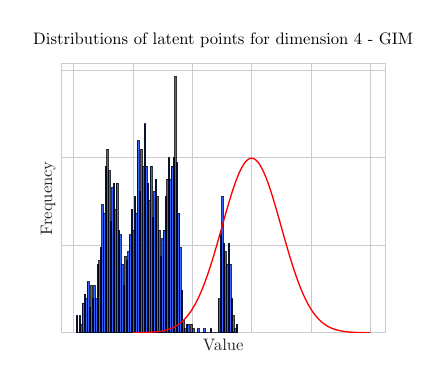
\begin{tikzpicture}[scale=0.6]

\definecolor{blue262255}{RGB}{2,62,255}
\definecolor{darkslategray38}{RGB}{38,38,38}
\definecolor{lightgray204}{RGB}{204,204,204}

\begin{axis}[
axis line style={lightgray204},
tick align=outside,
title={Distributions of latent points for dimension 4 - GIM},
x grid style={lightgray204},
xlabel=\textcolor{darkslategray38}{Value},
xmajorgrids,
xmajorticks=false,
xmin=-6.41184144020081, xmax=4.4958019733429,
xtick style={color=darkslategray38},
y grid style={lightgray204},
ylabel=\textcolor{darkslategray38}{Frequency},
ymajorgrids,
ymajorticks=false,
ymin=0, ymax=0.614785411616198,
ytick style={color=darkslategray38}
]
\draw[draw=black,fill=blue262255,opacity=0.8,line width=0.48pt] (axis cs:-5.91603946685791,0) rectangle (axis cs:-5.86156034469604,0.0390338235627163);
\draw[draw=black,fill=blue262255,opacity=0.8,line width=0.48pt] (axis cs:-5.86156034469604,0) rectangle (axis cs:-5.80708169937134,0);
\draw[draw=black,fill=blue262255,opacity=0.8,line width=0.48pt] (axis cs:-5.8070821762085,0) rectangle (axis cs:-5.75260305404663,0.0390338235627163);
\draw[draw=black,fill=blue262255,opacity=0.8,line width=0.48pt] (axis cs:-5.75260257720947,0) rectangle (axis cs:-5.69812393188477,0.0195170826077195);
\draw[draw=black,fill=blue262255,opacity=0.8,line width=0.48pt] (axis cs:-5.69812393188477,0) rectangle (axis cs:-5.6436448097229,0.0683091912347536);
\draw[draw=black,fill=blue262255,opacity=0.8,line width=0.48pt] (axis cs:-5.6436448097229,0) rectangle (axis cs:-5.58916616439819,0.0878268717347377);
\draw[draw=black,fill=blue262255,opacity=0.8,line width=0.48pt] (axis cs:-5.58916664123535,0) rectangle (axis cs:-5.53468751907349,0.0780676471254326);
\draw[draw=black,fill=blue262255,opacity=0.8,line width=0.48pt] (axis cs:-5.53468704223633,0) rectangle (axis cs:-5.48020839691162,0.117102495646317);
\draw[draw=black,fill=blue262255,opacity=0.8,line width=0.48pt] (axis cs:-5.48020839691162,0) rectangle (axis cs:-5.42572927474976,0.0585507353440745);
\draw[draw=black,fill=blue262255,opacity=0.8,line width=0.48pt] (axis cs:-5.42572927474976,0) rectangle (axis cs:-5.37125062942505,0.107343954342457);
\draw[draw=black,fill=blue262255,opacity=0.8,line width=0.48pt] (axis cs:-5.37125110626221,0) rectangle (axis cs:-5.31677198410034,0.0780676471254326);
\draw[draw=black,fill=blue262255,opacity=0.8,line width=0.48pt] (axis cs:-5.31677150726318,0) rectangle (axis cs:-5.26229286193848,0.107343954342457);
\draw[draw=black,fill=blue262255,opacity=0.8,line width=0.48pt] (axis cs:-5.26229286193848,0) rectangle (axis cs:-5.20781373977661,0.0780676471254326);
\draw[draw=black,fill=blue262255,opacity=0.8,line width=0.48pt] (axis cs:-5.20781373977661,0) rectangle (axis cs:-5.1533350944519,0.156136660861756);
\draw[draw=black,fill=blue262255,opacity=0.8,line width=0.48pt] (axis cs:-5.15333557128906,0) rectangle (axis cs:-5.0988564491272,0.165893750141544);
\draw[draw=black,fill=blue262255,opacity=0.8,line width=0.48pt] (axis cs:-5.09885597229004,0) rectangle (axis cs:-5.04437732696533,0.195170826077195);
\draw[draw=black,fill=blue262255,opacity=0.8,line width=0.48pt] (axis cs:-5.04437732696533,0) rectangle (axis cs:-4.98989820480347,0.292753676720372);
\draw[draw=black,fill=blue262255,opacity=0.8,line width=0.48pt] (axis cs:-4.98989820480347,0) rectangle (axis cs:-4.93541955947876,0.273239156508073);
\draw[draw=black,fill=blue262255,opacity=0.8,line width=0.48pt] (axis cs:-4.93542003631592,0) rectangle (axis cs:-4.88094091415405,0.380579779736484);
\draw[draw=black,fill=blue262255,opacity=0.8,line width=0.48pt] (axis cs:-4.88094043731689,0) rectangle (axis cs:-4.82646179199219,0.419617276065969);
\draw[draw=black,fill=blue262255,opacity=0.8,line width=0.48pt] (axis cs:-4.82646179199219,0) rectangle (axis cs:-4.77198266983032,0.370821323845805);
\draw[draw=black,fill=blue262255,opacity=0.8,line width=0.48pt] (axis cs:-4.77198266983032,0) rectangle (axis cs:-4.71750402450562,0.253722073900353);
\draw[draw=black,fill=blue262255,opacity=0.8,line width=0.48pt] (axis cs:-4.71750450134277,0) rectangle (axis cs:-4.66302537918091,0.331787500283089);
\draw[draw=black,fill=blue262255,opacity=0.8,line width=0.48pt] (axis cs:-4.66302490234375,0) rectangle (axis cs:-4.60854625701904,0.341548945635091);
\draw[draw=black,fill=blue262255,opacity=0.8,line width=0.48pt] (axis cs:-4.60854625701904,0) rectangle (axis cs:-4.55406713485718,0.282995220829693);
\draw[draw=black,fill=blue262255,opacity=0.8,line width=0.48pt] (axis cs:-4.55406713485718,0) rectangle (axis cs:-4.49958848953247,0.341548945635091);
\draw[draw=black,fill=blue262255,opacity=0.8,line width=0.48pt] (axis cs:-4.49958896636963,0) rectangle (axis cs:-4.44510984420776,0.234202941376298);
\draw[draw=black,fill=blue262255,opacity=0.8,line width=0.48pt] (axis cs:-4.44510936737061,0) rectangle (axis cs:-4.3906307220459,0.224446449988774);
\draw[draw=black,fill=blue262255,opacity=0.8,line width=0.48pt] (axis cs:-4.3906307220459,0) rectangle (axis cs:-4.33615159988403,0.156135294250865);
\draw[draw=black,fill=blue262255,opacity=0.8,line width=0.48pt] (axis cs:-4.33615159988403,0) rectangle (axis cs:-4.28167295455933,0.107343954342457);
\draw[draw=black,fill=blue262255,opacity=0.8,line width=0.48pt] (axis cs:-4.28167343139648,0) rectangle (axis cs:-4.22719430923462,0.175652206032223);
\draw[draw=black,fill=blue262255,opacity=0.8,line width=0.48pt] (axis cs:-4.22719383239746,0) rectangle (axis cs:-4.17271518707275,0.165895202165616);
\draw[draw=black,fill=blue262255,opacity=0.8,line width=0.48pt] (axis cs:-4.17271518707275,0) rectangle (axis cs:-4.11823606491089,0.185410661922903);
\draw[draw=black,fill=blue262255,opacity=0.8,line width=0.48pt] (axis cs:-4.11823606491089,0) rectangle (axis cs:-4.06375741958618,0.224446449988774);
\draw[draw=black,fill=blue262255,opacity=0.8,line width=0.48pt] (axis cs:-4.06375789642334,0) rectangle (axis cs:-4.00927877426147,0.282995220829693);
\draw[draw=black,fill=blue262255,opacity=0.8,line width=0.48pt] (axis cs:-4.00927829742432,0) rectangle (axis cs:-3.95479965209961,0.23420396632998);
\draw[draw=black,fill=blue262255,opacity=0.8,line width=0.48pt] (axis cs:-3.95479917526245,0) rectangle (axis cs:-3.90032052993774,0.31227195510664);
\draw[draw=black,fill=blue262255,opacity=0.8,line width=0.48pt] (axis cs:-3.90032052993774,0) rectangle (axis cs:-3.84584188461304,0.27323796071831);
\draw[draw=black,fill=blue262255,opacity=0.8,line width=0.48pt] (axis cs:-3.84584140777588,0) rectangle (axis cs:-3.79136276245117,0.439132436868713);
\draw[draw=black,fill=blue262255,opacity=0.8,line width=0.48pt] (axis cs:-3.79136276245117,0) rectangle (axis cs:-3.73688411712646,0.322030453703723);
\draw[draw=black,fill=blue262255,opacity=0.8,line width=0.48pt] (axis cs:-3.73688364028931,0) rectangle (axis cs:-3.6824049949646,0.419615439674548);
\draw[draw=black,fill=blue262255,opacity=0.8,line width=0.48pt] (axis cs:-3.6824049949646,0) rectangle (axis cs:-3.62792634963989,0.380581445286218);
\draw[draw=black,fill=blue262255,opacity=0.8,line width=0.48pt] (axis cs:-3.62792587280273,0) rectangle (axis cs:-3.57344722747803,0.478166431257043);
\draw[draw=black,fill=blue262255,opacity=0.8,line width=0.48pt] (axis cs:-3.57344722747803,0) rectangle (axis cs:-3.51896858215332,0.380581445286218);
\draw[draw=black,fill=blue262255,opacity=0.8,line width=0.48pt] (axis cs:-3.51896810531616,0) rectangle (axis cs:-3.46448945999146,0.341547450897888);
\draw[draw=black,fill=blue262255,opacity=0.8,line width=0.48pt] (axis cs:-3.46448945999146,0) rectangle (axis cs:-3.41001081466675,0.302513456509558);
\draw[draw=black,fill=blue262255,opacity=0.8,line width=0.48pt] (axis cs:-3.41001033782959,0) rectangle (axis cs:-3.35553169250488,0.380581445286218);
\draw[draw=black,fill=blue262255,opacity=0.8,line width=0.48pt] (axis cs:-3.35553169250488,0) rectangle (axis cs:-3.30105304718018,0.263479462121228);
\draw[draw=black,fill=blue262255,opacity=0.8,line width=0.48pt] (axis cs:-3.30105257034302,0) rectangle (axis cs:-3.24657392501831,0.322030453703723);
\draw[draw=black,fill=blue262255,opacity=0.8,line width=0.48pt] (axis cs:-3.24657392501831,0) rectangle (axis cs:-3.1920952796936,0.35130594949497);
\draw[draw=black,fill=blue262255,opacity=0.8,line width=0.48pt] (axis cs:-3.19209480285645,0) rectangle (axis cs:-3.13761615753174,0.31227195510664);
\draw[draw=black,fill=blue262255,opacity=0.8,line width=0.48pt] (axis cs:-3.13761615753174,0) rectangle (axis cs:-3.08313751220703,0.23420396632998);
\draw[draw=black,fill=blue262255,opacity=0.8,line width=0.48pt] (axis cs:-3.08313703536987,0) rectangle (axis cs:-3.02865839004517,0.175652974747485);
\draw[draw=black,fill=blue262255,opacity=0.8,line width=0.48pt] (axis cs:-3.02865839004517,0) rectangle (axis cs:-2.97417974472046,0.214686969135815);
\draw[draw=black,fill=blue262255,opacity=0.8,line width=0.48pt] (axis cs:-2.9741792678833,0) rectangle (axis cs:-2.91970062255859,0.23420396632998);
\draw[draw=black,fill=blue262255,opacity=0.8,line width=0.48pt] (axis cs:-2.91970062255859,0) rectangle (axis cs:-2.86522197723389,0.31227195510664);
\draw[draw=black,fill=blue262255,opacity=0.8,line width=0.48pt] (axis cs:-2.86522150039673,0) rectangle (axis cs:-2.81074285507202,0.35130594949497);
\draw[draw=black,fill=blue262255,opacity=0.8,line width=0.48pt] (axis cs:-2.81074285507202,0) rectangle (axis cs:-2.75626420974731,0.400098442480383);
\draw[draw=black,fill=blue262255,opacity=0.8,line width=0.48pt] (axis cs:-2.75626373291016,0) rectangle (axis cs:-2.70178508758545,0.35130594949497);
\draw[draw=black,fill=blue262255,opacity=0.8,line width=0.48pt] (axis cs:-2.70178508758545,0) rectangle (axis cs:-2.64730596542358,0.380579779736484);
\draw[draw=black,fill=blue262255,opacity=0.8,line width=0.48pt] (axis cs:-2.64730596542358,0) rectangle (axis cs:-2.59282732009888,0.400098442480383);
\draw[draw=black,fill=blue262255,opacity=0.8,line width=0.48pt] (axis cs:-2.59282684326172,0) rectangle (axis cs:-2.53834819793701,0.585509915824951);
\draw[draw=black,fill=blue262255,opacity=0.8,line width=0.48pt] (axis cs:-2.53834819793701,0) rectangle (axis cs:-2.4838695526123,0.390339943883301);
\draw[draw=black,fill=blue262255,opacity=0.8,line width=0.48pt] (axis cs:-2.48386907577515,0) rectangle (axis cs:-2.42939043045044,0.27323796071831);
\draw[draw=black,fill=blue262255,opacity=0.8,line width=0.48pt] (axis cs:-2.42939043045044,0) rectangle (axis cs:-2.37491178512573,0.19516997194165);
\draw[draw=black,fill=blue262255,opacity=0.8,line width=0.48pt] (axis cs:-2.37491130828857,0) rectangle (axis cs:-2.32043266296387,0.0975849859708251);
\draw[draw=black,fill=blue262255,opacity=0.8,line width=0.48pt] (axis cs:-2.32043266296387,0) rectangle (axis cs:-2.26595401763916,0.0292754957912475);
\draw[draw=black,fill=blue262255,opacity=0.8,line width=0.48pt] (axis cs:-2.265953540802,0) rectangle (axis cs:-2.21147489547729,0.00975849859708251);
\draw[draw=black,fill=blue262255,opacity=0.8,line width=0.48pt] (axis cs:-2.21147489547729,0) rectangle (axis cs:-2.15699625015259,0.019516997194165);
\draw[draw=black,fill=blue262255,opacity=0.8,line width=0.48pt] (axis cs:-2.15699577331543,0) rectangle (axis cs:-2.10251712799072,0.019516997194165);
\draw[draw=black,fill=blue262255,opacity=0.8,line width=0.48pt] (axis cs:-2.10251712799072,0) rectangle (axis cs:-2.04803848266602,0);
\draw[draw=black,fill=blue262255,opacity=0.8,line width=0.48pt] (axis cs:-2.04803800582886,0) rectangle (axis cs:-1.99355936050415,0.019516997194165);
\draw[draw=black,fill=blue262255,opacity=0.8,line width=0.48pt] (axis cs:-1.99355924129486,0) rectangle (axis cs:-1.93908059597015,0.00975849859708251);
\draw[draw=black,fill=blue262255,opacity=0.8,line width=0.48pt] (axis cs:-1.93908035755157,0) rectangle (axis cs:-1.88460171222687,0);
\draw[draw=black,fill=blue262255,opacity=0.8,line width=0.48pt] (axis cs:-1.88460147380829,0) rectangle (axis cs:-1.83012282848358,0);
\draw[draw=black,fill=blue262255,opacity=0.8,line width=0.48pt] (axis cs:-1.830122590065,0) rectangle (axis cs:-1.7756439447403,0.00975849859708251);
\draw[draw=black,fill=blue262255,opacity=0.8,line width=0.48pt] (axis cs:-1.77564370632172,0) rectangle (axis cs:-1.72116506099701,0);
\draw[draw=black,fill=blue262255,opacity=0.8,line width=0.48pt] (axis cs:-1.72116482257843,0) rectangle (axis cs:-1.66668617725372,0);
\draw[draw=black,fill=blue262255,opacity=0.8,line width=0.48pt] (axis cs:-1.66668593883514,0) rectangle (axis cs:-1.61220729351044,0);
\draw[draw=black,fill=blue262255,opacity=0.8,line width=0.48pt] (axis cs:-1.61220705509186,0) rectangle (axis cs:-1.55772840976715,0.00975849859708251);
\draw[draw=black,fill=blue262255,opacity=0.8,line width=0.48pt] (axis cs:-1.55772817134857,0) rectangle (axis cs:-1.50324952602386,0);
\draw[draw=black,fill=blue262255,opacity=0.8,line width=0.48pt] (axis cs:-1.50324928760529,0) rectangle (axis cs:-1.44877064228058,0);
\draw[draw=black,fill=blue262255,opacity=0.8,line width=0.48pt] (axis cs:-1.448770403862,0) rectangle (axis cs:-1.39429175853729,0);
\draw[draw=black,fill=blue262255,opacity=0.8,line width=0.48pt] (axis cs:-1.39429152011871,0) rectangle (axis cs:-1.33981287479401,0.00975849859708251);
\draw[draw=black,fill=blue262255,opacity=0.8,line width=0.48pt] (axis cs:-1.33981263637543,0) rectangle (axis cs:-1.28533399105072,0);
\draw[draw=black,fill=blue262255,opacity=0.8,line width=0.48pt] (axis cs:-1.28533375263214,0) rectangle (axis cs:-1.23085510730743,0);
\draw[draw=black,fill=blue262255,opacity=0.8,line width=0.48pt] (axis cs:-1.23085486888885,0) rectangle (axis cs:-1.17637622356415,0);
\draw[draw=black,fill=blue262255,opacity=0.8,line width=0.48pt] (axis cs:-1.17637598514557,0) rectangle (axis cs:-1.12189733982086,0);
\draw[draw=black,fill=blue262255,opacity=0.8,line width=0.48pt] (axis cs:-1.12189710140228,0) rectangle (axis cs:-1.06741845607758,0.0780679887766601);
\draw[draw=black,fill=blue262255,opacity=0.8,line width=0.48pt] (axis cs:-1.067418217659,0) rectangle (axis cs:-1.01293957233429,0.224445467732898);
\draw[draw=black,fill=blue262255,opacity=0.8,line width=0.48pt] (axis cs:-1.01293957233429,0) rectangle (axis cs:-0.958460450172424,0.312271613454292);
\draw[draw=black,fill=blue262255,opacity=0.8,line width=0.48pt] (axis cs:-0.95846039056778,0) rectangle (axis cs:-0.903981745243073,0.204928470538733);
\draw[draw=black,fill=blue262255,opacity=0.8,line width=0.48pt] (axis cs:-0.903981506824493,0) rectangle (axis cs:-0.849502861499786,0.185411473344568);
\draw[draw=black,fill=blue262255,opacity=0.8,line width=0.48pt] (axis cs:-0.849502623081207,0) rectangle (axis cs:-0.7950239777565,0.15613597755332);
\draw[draw=black,fill=blue262255,opacity=0.8,line width=0.48pt] (axis cs:-0.795023918151855,0) rectangle (axis cs:-0.74054479598999,0.204928246329379);
\draw[draw=black,fill=blue262255,opacity=0.8,line width=0.48pt] (axis cs:-0.74054479598999,0) rectangle (axis cs:-0.686066150665283,0.15613597755332);
\draw[draw=black,fill=blue262255,opacity=0.8,line width=0.48pt] (axis cs:-0.686065912246704,0) rectangle (axis cs:-0.631587266921997,0.0780679887766601);
\draw[draw=black,fill=blue262255,opacity=0.8,line width=0.48pt] (axis cs:-0.631587028503418,0) rectangle (axis cs:-0.577108383178711,0.03903399438833);
\draw[draw=black,fill=blue262255,opacity=0.8,line width=0.48pt] (axis cs:-0.577108144760132,0) rectangle (axis cs:-0.522629499435425,0.00975849859708251);
\draw[draw=black,fill=blue262255,opacity=0.8,line width=0.48pt] (axis cs:-0.522629261016846,0) rectangle (axis cs:-0.468150615692139,0.019516997194165);
\addplot [thick, red]
table {%
-4 0.000133830225764885
-3.99199199199199 0.000138182046410498
-3.98398398398398 0.000142666228042307
-3.97597597597598 0.000147286481503254
-3.96796796796797 0.000152046611333821
-3.95995995995996 0.000156950517814782
-3.95195195195195 0.00016200219904485
-3.94394394394394 0.00016720575305353
-3.93593593593594 0.000172565379949496
-3.92792792792793 0.00017808538410479
-3.91991991991992 0.000183770176375138
-3.91191191191191 0.000189624276356684
-3.9039039039039 0.000195652314679408
-3.8958958958959 0.000201859035337517
-3.88788788788789 0.000208249298057069
-3.87987987987988 0.000214828080701088
-3.87187187187187 0.000221600481712426
-3.86386386386386 0.0002285717225946
-3.85585585585586 0.000235747150430845
-3.84784784784785 0.000243132240441603
-3.83983983983984 0.000250732598580649
-3.83183183183183 0.000258553964170059
-3.82382382382382 0.000266602212574213
-3.81581581581582 0.000274883357912987
-3.80780780780781 0.000283403555814325
-3.7997997997998 0.000292169106206322
-3.79179179179179 0.000301186456148957
-3.78378378378378 0.0003104622027056
-3.77577577577578 0.000320003095854415
-3.76776776776777 0.000329816041439723
-3.75975975975976 0.000339908104163431
-3.75175175175175 0.00035028651061658
-3.74374374374374 0.000360958652351047
-3.73573573573574 0.000371932088991451
-3.72772772772773 0.000383214551387261
-3.71971971971972 0.000394813944805093
-3.71171171171171 0.000406738352161197
-3.7037037037037 0.000418996037294058
-3.6956956956957 0.00043159544827708
-3.68768768768769 0.00044454522077123
-3.67967967967968 0.000457854181417586
-3.67167167167167 0.000471531351269624
-3.66366366366366 0.000485585949265103
-3.65565565565566 0.000500027395737409
-3.64764764764765 0.000514865315966112
-3.63963963963964 0.000530109543766577
-3.63163163163163 0.000545770125118336
-3.62362362362362 0.000561857321831991
-3.61561561561562 0.00057838161525435
-3.60760760760761 0.000595353710011453
-3.5995995995996 0.000612784537789192
-3.59159159159159 0.000630685261151105
-3.58358358358358 0.000649067277392973
-3.57557557557558 0.000667942222433796
-3.56756756756757 0.000687321974742665
-3.55955955955956 0.000707218659301081
-3.55155155155155 0.000727644651600166
-3.54354354354354 0.000748612581672245
-3.53553553553554 0.000770135338156225
-3.52752752752753 0.000792226072396121
-3.51951951951952 0.00081489820257214
-3.51151151151151 0.000838165417863603
-3.5035035035035 0.000862041682643007
-3.4954954954955 0.000886541240700502
-3.48748748748749 0.00091167861949796
-3.47947947947948 0.000937468634451866
-3.47147147147147 0.000963926393244149
-3.46346346346346 0.000991067300160059
-3.45545545545546 0.0010189070604522
-3.44744744744745 0.00104746168472971
-3.43943943943944 0.0010767474933716
-3.43143143143143 0.00110678112096323
-3.42342342342342 0.00113757952075483
-3.41541541541542 0.00116915996914087
-3.40740740740741 0.00120154007015926
-3.3993993993994 0.00123473776000907
-3.39139139139139 0.00126877131158549
-3.38338338338338 0.00130365933903088
-3.37537537537538 0.00133942080230046
-3.36736736736737 0.00137607501174126
-3.35935935935936 0.001413641632683
-3.35135135135135 0.00145214069003938
-3.34334334334334 0.0014915925729182
-3.33533533533534 0.00153201803923895
-3.32732732732733 0.00157343822035606
-3.31931931931932 0.00161587462568624
-3.31131131131131 0.00165934914733831
-3.3033033033033 0.00170388406474362
-3.2952952952953 0.00174950204928538
-3.28728728728729 0.00179622616892505
-3.27927927927928 0.00184407989282385
-3.27127127127127 0.00189308709595757
-3.26326326326326 0.00194327206372255
-3.25525525525526 0.00199465949653091
-3.24724724724725 0.00204727451439301
-3.23923923923924 0.00210114266148476
-3.23123123123123 0.00215628991069791
-3.22322322322322 0.00221274266817093
-3.21521521521522 0.00227052777779815
-3.20720720720721 0.00232967252571501
-3.1991991991992 0.00239020464475689
-3.19119119119119 0.00245215231888918
-3.18318318318318 0.00251554418760605
-3.17517517517518 0.00258040935029545
-3.16716716716717 0.00264677737056774
-3.15915915915916 0.00271467828054534
-3.15115115115115 0.00278414258511061
-3.14314314314314 0.00285520126610952
-3.13513513513514 0.00292788578650791
-3.12712712712713 0.00300222809449793
-3.11911911911912 0.00307826062755151
-3.11111111111111 0.00315601631641804
-3.1031031031031 0.00323552858906328
-3.0950950950951 0.00331683137454643
-3.08708708708709 0.00339995910683238
-3.07907907907908 0.00348494672853595
-3.07107107107107 0.00357182969459489
-3.06306306306306 0.00366064397586864
-3.05505505505506 0.00375142606265932
-3.04704704704705 0.00384421296815189
-3.03903903903904 0.00393904223176991
-3.03103103103103 0.00403595192244368
-3.02302302302302 0.0041349806417872
-3.01501501501502 0.00423616752718052
-3.00700700700701 0.00433955225475399
-2.998998998999 0.00444517504227068
-2.99099099099099 0.00455307665190355
-2.98298298298298 0.00466329839290368
-2.97497497497497 0.00477588212415564
-2.96696696696697 0.00489087025661667
-2.95895895895896 0.00500830575563558
-2.95095095095095 0.00512823214314763
-2.94294294294294 0.00525069349974172
-2.93493493493493 0.00537573446659573
-2.92692692692693 0.00550340024727644
-2.91891891891892 0.00563373660939975
-2.91091091091091 0.0057667898861475
-2.9029029029029 0.00590260697763674
-2.89489489489489 0.00604123535213746
-2.88688688688689 0.00618272304713484
-2.87887887887888 0.00632711867023164
-2.87087087087087 0.00647447139988703
-2.86286286286286 0.00662483098598741
-2.85485485485485 0.0067782477502453
-2.84684684684685 0.0069347725864219
-2.83883883883884 0.00709445696036946
-2.83083083083083 0.00725735290988893
-2.82282282282282 0.00742351304439893
-2.81481481481481 0.00759299054441176
-2.80680680680681 0.0077658391608121
-2.7987987987988 0.00794211321393437
-2.79079079079079 0.00812186759243432
-2.78278278278278 0.00830515775195071
-2.77477477477477 0.00849203971355293
-2.76676676676677 0.00868257006197001
-2.75875875875876 0.00887680594359712
-2.75075075075075 0.00907480506427511
-2.74274274274274 0.00927662568683898
-2.73473473473473 0.00948232662843099
-2.72672672672673 0.00969196725757422
-2.71871871871872 0.00990560749100246
-2.71071071071071 0.0101233077902421
-2.7027027027027 0.0103451291579421
-2.69469469469469 0.0105711331339476
-2.68668668668669 0.0108013817911136
-2.67867867867868 0.011035937730854
-2.67067067067067 0.0112748640784219
-2.66266266266266 0.0115182244779185
-2.65465465465465 0.0117660830870247
-2.64664664664665 0.0120185045714526
-2.63863863863864 0.0122755540991133
-2.63063063063063 0.0125372973339956
-2.62262262262262 0.0128038004297541
-2.61461461461461 0.0130751300230007
-2.60660660660661 0.0133513532262973
-2.5985985985986 0.0136325376208454
-2.59059059059059 0.0139187512488692
-2.58258258258258 0.014210062605689
-2.57457457457457 0.0145065406314803
-2.56656656656657 0.0148082547027168
-2.55855855855856 0.0151152746232934
-2.55055055055055 0.0154276706153247
-2.54254254254254 0.0157455133096184
-2.53453453453453 0.0160688737358178
-2.52652652652653 0.016397823312213
-2.51851851851852 0.0167324338352151
-2.51051051051051 0.0170727774684938
-2.5025025025025 0.0174189267317727
-2.49449449449449 0.0177709544892815
-2.48648648648649 0.0181289339378627
-2.47847847847848 0.0184929385947284
-2.47047047047047 0.0188630422848682
-2.46246246246246 0.0192393191281025
-2.45445445445445 0.0196218435257817
-2.44644644644645 0.0200106901471285
-2.43843843843844 0.020405933915221
-2.43043043043043 0.0208076499926159
-2.42242242242242 0.0212159137666093
-2.41441441441441 0.0216308008341344
-2.40640640640641 0.0220523869862944
-2.3983983983984 0.0224807481925294
-2.39039039039039 0.022915960584417
-2.38238238238238 0.0233581004391047
-2.37437437437437 0.023807244162374
-2.36636636636637 0.0242634682713357
-2.35835835835836 0.0247268493767558
-2.35035035035035 0.0251974641650118
-2.34234234234234 0.0256753893796796
-2.33433433433433 0.0261607018027501
-2.32632632632633 0.0266534782354775
-2.31831831831832 0.0271537954788581
-2.31031031031031 0.0276617303137407
-2.3023023023023 0.0281773594805703
-2.29429429429429 0.0287007596587648
-2.28628628628629 0.0292320074457259
-2.27827827827828 0.029771179335487
-2.27027027027027 0.0303183516969979
-2.26226226226226 0.0308736007520491
-2.25425425425425 0.0314370025528369
-2.24624624624625 0.0320086329591723
-2.23823823823824 0.0325885676153351
-2.23023023023023 0.0331768819265761
-2.22222222222222 0.0337736510352706
-2.21421421421421 0.0343789497967251
-2.20620620620621 0.0349928527546413
-2.1981981981982 0.0356154341162401
-2.19019019019019 0.0362467677270497
-2.18218218218218 0.0368869270453615
-2.17417417417417 0.0375359851163567
-2.16616616616617 0.03819401454591
-2.15815815815816 0.0388610874740724
-2.15015015015015 0.03953727554824
-2.14214214214214 0.0402226498960119
-2.13413413413413 0.0409172810977437
-2.12612612612613 0.0416212391588003
-2.11811811811812 0.0423345934815158
-2.11011011011011 0.0430574128368641
-2.1021021021021 0.043789765335848
-2.09409409409409 0.0445317184006117
-2.08608608608609 0.0452833387352837
-2.07807807807808 0.0460446922965577
-2.07007007007007 0.0468158442640166
-2.06206206206206 0.0475968590102091
-2.05405405405405 0.0483878000704834
-2.04604604604605 0.0491887301125894
-2.03803803803804 0.0499997109060533
-2.03003003003003 0.0508208032913361
-2.02202202202202 0.0516520671487823
-2.01401401401401 0.0524935613673682
-2.00600600600601 0.053345343813258
-1.997997997998 0.0542074712981785
-1.98998998998999 0.0550799995476186
-1.98198198198198 0.0559629831688668
-1.97397397397397 0.0568564756188931
-1.96596596596597 0.0577605291720876
-1.95795795795796 0.0586751948878651
-1.94994994994995 0.0596005225781457
-1.94194194194194 0.0605365607747232
-1.93393393393393 0.0614833566965309
-1.92592592592593 0.062440956216817
-1.91791791791792 0.06340940383024
-1.90990990990991 0.0643887426198963
-1.9019019019019 0.0653790142242912
-1.89389389389389 0.0663802588042656
-1.88588588588589 0.0673925150098903
-1.87787787787788 0.0684158199473405
-1.86986986986987 0.0694502091457625
-1.86186186186186 0.0704957165241465
-1.85385385385385 0.0715523743582165
-1.84584584584585 0.0726202132473521
-1.83783783783784 0.0736992620815557
-1.82982982982983 0.0747895480084762
-1.82182182182182 0.0758910964005057
-1.81381381381381 0.0770039308219614
-1.80580580580581 0.0781280729963669
-1.7977977977978 0.0792635427738473
-1.78978978978979 0.0804103580986525
-1.78178178178178 0.0815685349768227
-1.77377377377377 0.0827380874440109
-1.76576576576577 0.0839190275334777
-1.75775775775776 0.0851113652442723
-1.74974974974975 0.086315108509615
-1.74174174174174 0.0875302631654975
-1.73373373373373 0.0887568329195139
-1.72572572572573 0.0899948193199405
-1.71771771771772 0.0912442217250772
-1.70970970970971 0.0925050372728685
-1.7017017017017 0.0937772608508177
-1.69369369369369 0.0950608850662112
-1.68568568568569 0.0963559002166691
-1.67767767767768 0.0976622942610365
-1.66966966966967 0.0989800527906321
-1.66166166166166 0.100309159000872
-1.65365365365365 0.10164959366328
-1.64564564564565 0.103001335097907
-1.63763763763764 0.10436435914617
-1.62962962962963 0.105738639144131
-1.62162162162162 0.107124145896225
-1.61361361361361 0.108520847649465
-1.60560560560561 0.10992871006813
-1.5975975975976 0.111347696208955
-1.58958958958959 0.112777766496842
-1.58158158158158 0.114218878701105
-1.57357357357357 0.115670987912262
-1.56556556556557 0.117134046519405
-1.55755755755756 0.11860800418814
-1.54954954954955 0.120092807839133
-1.54154154154154 0.121588401627275
-1.53353353353353 0.123094726921466
-1.52552552552553 0.124611722285057
-1.51751751751752 0.12613932345695
-1.50950950950951 0.127677463333369
-1.5015015015015 0.129226071950339
-1.49349349349349 0.130785076466857
-1.48548548548549 0.132354401148798
-1.47747747747748 0.133933967353555
-1.46946946946947 0.13552369351543
-1.46146146146146 0.137123495131801
-1.45345345345345 0.13873328475006
-1.44544544544545 0.140352971955359
-1.43743743743744 0.141982463359159
-1.42942942942943 0.143621662588612
-1.42142142142142 0.14527047027677
-1.41341341341341 0.146928784053658
-1.40540540540541 0.148596498538208
-1.3973973973974 0.150273505331067
-1.38938938938939 0.151959693008306
-1.38138138138138 0.153654947116025
-1.37337337337337 0.155359150165875
-1.36536536536537 0.157072181631514
-1.35735735735736 0.158793917945997
-1.34934934934935 0.160524232500121
-1.34134134134134 0.16226299564173
-1.33333333333333 0.164010074675994
-1.32532532532533 0.165765333866673
-1.31731731731732 0.167528634438376
-1.30930930930931 0.169299834579821
-1.3013013013013 0.17107878944811
-1.29329329329329 0.172865351174024
-1.28528528528529 0.174659368868355
-1.27727727727728 0.176460688629273
-1.26926926926927 0.178269153550739
-1.26126126126126 0.180084603731981
-1.25325325325325 0.181906876288021
-1.24524524524525 0.183735805361283
-1.23723723723724 0.185571222134271
-1.22922922922923 0.187412954843324
-1.22122122122122 0.18926082879347
-1.21321321321321 0.191114666374361
-1.20520520520521 0.192974287077311
-1.1971971971972 0.194839507513435
-1.18918918918919 0.19671014143289
-1.18118118118118 0.198585999745227
-1.17317317317317 0.200466890540856
-1.16516516516517 0.202352619113618
-1.15715715715716 0.204242987984477
-1.14914914914915 0.206137796926331
-1.14114114114114 0.208036842989938
-1.13313313313313 0.209939920530956
-1.12512512512513 0.21184682123811
-1.11711711711712 0.21375733416247
-1.10910910910911 0.215671245747847
-1.1011011011011 0.217588339862305
-1.09309309309309 0.219508397830784
-1.08508508508509 0.221431198468836
-1.07707707707708 0.223356518117463
-1.06906906906907 0.225284130679063
-1.06106106106106 0.22721380765447
-1.05305305305305 0.229145318181096
-1.04504504504505 0.231078429072154
-1.03703703703704 0.233012904856966
-1.02902902902903 0.234948507822352
-1.02102102102102 0.236884998055083
-1.01301301301301 0.238822133485401
-1.00500500500501 0.24075966993159
-0.996996996996997 0.242697361145593
-0.988988988988989 0.244634958859672
-0.980980980980981 0.246572212834085
-0.972972972972973 0.248508870905785
-0.964964964964965 0.250444679038131
-0.956956956956957 0.252379381371581
-0.948948948948949 0.254312720275385
-0.940940940940941 0.256244436400228
-0.932932932932933 0.258174268731856
-0.924924924924925 0.260101954645624
-0.916916916916917 0.262027229961987
-0.908908908908909 0.263949829002911
-0.900900900900901 0.265869484649172
-0.892892892892893 0.267785928398552
-0.884884884884885 0.269698890424904
-0.876876876876877 0.271608099638066
-0.868868868868869 0.273513283744617
-0.860860860860861 0.275414169309444
-0.852852852852853 0.277310481818125
-0.844844844844845 0.279201945740075
-0.836836836836837 0.281088284592474
-0.828828828828829 0.28296922100493
-0.820820820820821 0.284844476784867
-0.812812812812813 0.286713772983616
-0.804804804804805 0.288576829963198
-0.796796796796797 0.290433367463758
-0.788788788788789 0.292283104671645
-0.780780780780781 0.294125760288111
-0.772772772772773 0.295961052598604
-0.764764764764765 0.29778869954263
-0.756756756756757 0.299608418784177
-0.748748748748749 0.301419927782648
-0.740740740740741 0.303222943864308
-0.732732732732733 0.305017184294205
-0.724724724724725 0.306802366348536
-0.716716716716717 0.308578207387456
-0.708708708708709 0.310344424928268
-0.700700700700701 0.312100736719007
-0.692692692692693 0.313846860812361
-0.684684684684685 0.31558251563992
-0.676676676676677 0.317307420086723
-0.668668668668669 0.319021293566066
-0.660660660660661 0.320723856094559
-0.652652652652653 0.322414828367396
-0.644644644644645 0.324093931833804
-0.636636636636636 0.325760888772662
-0.628628628628629 0.327415422368237
-0.620620620620621 0.329057256786028
-0.612612612612613 0.330686117248681
-0.604604604604605 0.33230173011195
-0.596596596596596 0.333903822940662
-0.588588588588589 0.335492124584683
-0.580580580580581 0.337066365254824
-0.572572572572573 0.338626276598684
-0.564564564564565 0.340171591776383
-0.556556556556556 0.341702045536168
-0.548548548548549 0.343217374289848
-0.54054054054054 0.344717316188045
-0.532532532532533 0.346201611195215
-0.524524524524525 0.347670001164422
-0.516516516516516 0.349122229911825
-0.508508508508509 0.350558043290856
-0.5005005005005 0.351977189266054
-0.492492492492492 0.353379417986526
-0.484484484484485 0.354764481859011
-0.476476476476476 0.356132135620502
-0.468468468468469 0.357482136410418
-0.46046046046046 0.358814243842273
-0.452452452452452 0.360128220074839
-0.444444444444445 0.361423829882744
-0.436436436436436 0.362700840726495
-0.428428428428429 0.363959022821904
-0.42042042042042 0.365198149208855
-0.412412412412412 0.366417995819425
-0.404404404404405 0.3676183415453
-0.396396396396396 0.368798968304465
-0.388388388388389 0.369959661107154
-0.38038038038038 0.37110020812101
-0.372372372372372 0.372220400735444
-0.364364364364365 0.373320033625156
-0.356356356356356 0.374398904812801
-0.348348348348348 0.375456815730761
-0.34034034034034 0.376493571282005
-0.332332332332332 0.377508979900006
-0.324324324324325 0.378502853607702
-0.316316316316316 0.379475008075448
-0.308308308308308 0.380425262677969
-0.3003003003003 0.38135344055026
-0.292292292292292 0.382259368642425
-0.284284284284285 0.38314287777343
-0.276276276276276 0.384003802683735
-0.268268268268268 0.3848419820868
-0.26026026026026 0.385657258719425
-0.252252252252252 0.386449479390916
-0.244244244244244 0.387218495031049
-0.236236236236236 0.387964160736805
-0.228228228228228 0.38868633581787
-0.22022022022022 0.389384883840873
-0.212212212212212 0.390059672672329
-0.204204204204204 0.390710574520297
-0.196196196196196 0.391337465974705
-0.188188188188188 0.39194022804635
-0.18018018018018 0.392518746204527
-0.172172172172172 0.393072910413305
-0.164164164164164 0.393602615166401
-0.156156156156156 0.394107759520658
-0.148148148148148 0.394588247128102
-0.14014014014014 0.395043986266573
-0.132132132132132 0.3954748898689
-0.124124124124124 0.395880875550626
-0.116116116116116 0.396261865636259
-0.108108108108108 0.396617787184037
-0.1001001001001 0.396948572009207
-0.0920920920920922 0.397254156705792
-0.084084084084084 0.397534482666846
-0.0760760760760761 0.39778949610319
-0.0680680680680683 0.39801914806061
-0.06006006006006 0.398223394435522
-0.0520520520520522 0.398402195989086
-0.0440440440440439 0.398555518359772
-0.0360360360360361 0.398683332074364
-0.0280280280280278 0.398785612557403
-0.02002002002002 0.398862340139061
-0.0120120120120122 0.398913500061449
-0.00400400400400391 0.398939082483343
0.00400400400400436 0.398939082483343
0.0120120120120122 0.398913500061449
0.02002002002002 0.398862340139061
0.0280280280280278 0.398785612557403
0.0360360360360357 0.398683332074364
0.0440440440440444 0.398555518359772
0.0520520520520522 0.398402195989086
0.06006006006006 0.398223394435522
0.0680680680680679 0.39801914806061
0.0760760760760757 0.39778949610319
0.0840840840840844 0.397534482666846
0.0920920920920922 0.397254156705792
0.1001001001001 0.396948572009207
0.108108108108108 0.396617787184037
0.116116116116116 0.396261865636259
0.124124124124124 0.395880875550626
0.132132132132132 0.3954748898689
0.14014014014014 0.395043986266573
0.148148148148148 0.394588247128102
0.156156156156156 0.394107759520658
0.164164164164164 0.393602615166401
0.172172172172172 0.393072910413305
0.18018018018018 0.392518746204527
0.188188188188188 0.39194022804635
0.196196196196196 0.391337465974705
0.204204204204204 0.390710574520297
0.212212212212212 0.390059672672329
0.22022022022022 0.389384883840873
0.228228228228228 0.388686335817871
0.236236236236236 0.387964160736805
0.244244244244245 0.387218495031049
0.252252252252252 0.386449479390916
0.26026026026026 0.385657258719425
0.268268268268268 0.3848419820868
0.276276276276276 0.384003802683735
0.284284284284285 0.38314287777343
0.292292292292292 0.382259368642425
0.3003003003003 0.38135344055026
0.308308308308308 0.380425262677969
0.316316316316316 0.379475008075448
0.324324324324325 0.378502853607702
0.332332332332332 0.377508979900006
0.34034034034034 0.376493571282005
0.348348348348348 0.375456815730762
0.356356356356356 0.374398904812801
0.364364364364365 0.373320033625156
0.372372372372372 0.372220400735444
0.38038038038038 0.37110020812101
0.388388388388388 0.369959661107154
0.396396396396397 0.368798968304465
0.404404404404405 0.3676183415453
0.412412412412412 0.366417995819425
0.42042042042042 0.365198149208855
0.428428428428428 0.363959022821904
0.436436436436437 0.362700840726495
0.444444444444445 0.361423829882744
0.452452452452452 0.360128220074839
0.46046046046046 0.358814243842273
0.468468468468468 0.357482136410418
0.476476476476477 0.356132135620502
0.484484484484485 0.354764481859011
0.492492492492492 0.353379417986526
0.5005005005005 0.351977189266054
0.508508508508508 0.350558043290856
0.516516516516517 0.349122229911825
0.524524524524525 0.347670001164422
0.532532532532533 0.346201611195215
0.54054054054054 0.344717316188045
0.548548548548548 0.343217374289848
0.556556556556557 0.341702045536168
0.564564564564565 0.340171591776383
0.572572572572573 0.338626276598684
0.58058058058058 0.337066365254824
0.588588588588588 0.335492124584683
0.596596596596597 0.333903822940662
0.604604604604605 0.33230173011195
0.612612612612613 0.330686117248681
0.62062062062062 0.329057256786028
0.628628628628628 0.327415422368237
0.636636636636637 0.325760888772662
0.644644644644645 0.324093931833804
0.652652652652653 0.322414828367396
0.66066066066066 0.32072385609456
0.668668668668668 0.319021293566066
0.676676676676677 0.317307420086723
0.684684684684685 0.31558251563992
0.692692692692693 0.313846860812361
0.7007007007007 0.312100736719007
0.708708708708708 0.310344424928268
0.716716716716717 0.308578207387456
0.724724724724725 0.306802366348536
0.732732732732733 0.305017184294205
0.74074074074074 0.303222943864308
0.748748748748748 0.301419927782648
0.756756756756757 0.299608418784177
0.764764764764765 0.29778869954263
0.772772772772773 0.295961052598604
0.780780780780781 0.294125760288111
0.788788788788788 0.292283104671645
0.796796796796797 0.290433367463758
0.804804804804805 0.288576829963198
0.812812812812813 0.286713772983616
0.820820820820821 0.284844476784867
0.828828828828828 0.282969221004931
0.836836836836837 0.281088284592474
0.844844844844845 0.279201945740075
0.852852852852853 0.277310481818125
0.860860860860861 0.275414169309444
0.868868868868869 0.273513283744617
0.876876876876877 0.271608099638066
0.884884884884885 0.269698890424904
0.892892892892893 0.267785928398552
0.900900900900901 0.265869484649172
0.908908908908909 0.263949829002911
0.916916916916917 0.262027229961987
0.924924924924925 0.260101954645624
0.932932932932933 0.258174268731856
0.940940940940941 0.256244436400228
0.948948948948949 0.254312720275384
0.956956956956957 0.252379381371581
0.964964964964965 0.250444679038131
0.972972972972973 0.248508870905785
0.980980980980981 0.246572212834085
0.988988988988989 0.244634958859672
0.996996996996997 0.242697361145593
1.00500500500501 0.24075966993159
1.01301301301301 0.238822133485401
1.02102102102102 0.236884998055083
1.02902902902903 0.234948507822352
1.03703703703704 0.233012904856966
1.04504504504505 0.231078429072154
1.05305305305305 0.229145318181096
1.06106106106106 0.22721380765447
1.06906906906907 0.225284130679062
1.07707707707708 0.223356518117463
1.08508508508509 0.221431198468836
1.09309309309309 0.219508397830784
1.1011011011011 0.217588339862305
1.10910910910911 0.215671245747847
1.11711711711712 0.21375733416247
1.12512512512513 0.21184682123811
1.13313313313313 0.209939920530956
1.14114114114114 0.208036842989938
1.14914914914915 0.206137796926331
1.15715715715716 0.204242987984477
1.16516516516517 0.202352619113618
1.17317317317317 0.200466890540856
1.18118118118118 0.198585999745228
1.18918918918919 0.19671014143289
1.1971971971972 0.194839507513435
1.20520520520521 0.192974287077311
1.21321321321321 0.191114666374361
1.22122122122122 0.18926082879347
1.22922922922923 0.187412954843324
1.23723723723724 0.185571222134271
1.24524524524525 0.183735805361283
1.25325325325325 0.181906876288021
1.26126126126126 0.180084603731981
1.26926926926927 0.178269153550739
1.27727727727728 0.176460688629273
1.28528528528529 0.174659368868355
1.29329329329329 0.172865351174024
1.3013013013013 0.17107878944811
1.30930930930931 0.169299834579821
1.31731731731732 0.167528634438376
1.32532532532533 0.165765333866673
1.33333333333333 0.164010074675994
1.34134134134134 0.16226299564173
1.34934934934935 0.160524232500121
1.35735735735736 0.158793917945997
1.36536536536537 0.157072181631514
1.37337337337337 0.155359150165875
1.38138138138138 0.153654947116025
1.38938938938939 0.151959693008306
1.3973973973974 0.150273505331067
1.40540540540541 0.148596498538208
1.41341341341341 0.146928784053658
1.42142142142142 0.14527047027677
1.42942942942943 0.143621662588612
1.43743743743744 0.141982463359159
1.44544544544545 0.140352971955359
1.45345345345345 0.13873328475006
1.46146146146146 0.137123495131801
1.46946946946947 0.13552369351543
1.47747747747748 0.133933967353555
1.48548548548549 0.132354401148798
1.49349349349349 0.130785076466857
1.5015015015015 0.129226071950339
1.50950950950951 0.127677463333369
1.51751751751752 0.12613932345695
1.52552552552553 0.124611722285057
1.53353353353353 0.123094726921466
1.54154154154154 0.121588401627275
1.54954954954955 0.120092807839133
1.55755755755756 0.11860800418814
1.56556556556557 0.117134046519405
1.57357357357357 0.115670987912262
1.58158158158158 0.114218878701105
1.58958958958959 0.112777766496842
1.5975975975976 0.111347696208955
1.60560560560561 0.10992871006813
1.61361361361361 0.108520847649465
1.62162162162162 0.107124145896225
1.62962962962963 0.105738639144131
1.63763763763764 0.10436435914617
1.64564564564565 0.103001335097907
1.65365365365365 0.10164959366328
1.66166166166166 0.100309159000872
1.66966966966967 0.0989800527906321
1.67767767767768 0.0976622942610365
1.68568568568569 0.0963559002166692
1.69369369369369 0.0950608850662112
1.7017017017017 0.0937772608508176
1.70970970970971 0.0925050372728685
1.71771771771772 0.0912442217250772
1.72572572572573 0.0899948193199405
1.73373373373373 0.088756832919514
1.74174174174174 0.0875302631654974
1.74974974974975 0.086315108509615
1.75775775775776 0.0851113652442723
1.76576576576577 0.0839190275334778
1.77377377377377 0.082738087444011
1.78178178178178 0.0815685349768226
1.78978978978979 0.0804103580986525
1.7977977977978 0.0792635427738473
1.80580580580581 0.0781280729963669
1.81381381381381 0.0770039308219615
1.82182182182182 0.0758910964005057
1.82982982982983 0.0747895480084762
1.83783783783784 0.0736992620815557
1.84584584584585 0.0726202132473522
1.85385385385385 0.0715523743582165
1.86186186186186 0.0704957165241465
1.86986986986987 0.0694502091457625
1.87787787787788 0.0684158199473405
1.88588588588589 0.0673925150098903
1.89389389389389 0.0663802588042655
1.9019019019019 0.0653790142242912
1.90990990990991 0.0643887426198963
1.91791791791792 0.06340940383024
1.92592592592593 0.0624409562168171
1.93393393393393 0.0614833566965309
1.94194194194194 0.0605365607747232
1.94994994994995 0.0596005225781457
1.95795795795796 0.0586751948878651
1.96596596596597 0.0577605291720876
1.97397397397397 0.056856475618893
1.98198198198198 0.0559629831688668
1.98998998998999 0.0550799995476186
1.997997997998 0.0542074712981785
2.00600600600601 0.0533453438132581
2.01401401401401 0.0524935613673681
2.02202202202202 0.0516520671487823
2.03003003003003 0.0508208032913361
2.03803803803804 0.0499997109060533
2.04604604604605 0.0491887301125894
2.05405405405405 0.0483878000704834
2.06206206206206 0.0475968590102091
2.07007007007007 0.0468158442640166
2.07807807807808 0.0460446922965577
2.08608608608609 0.0452833387352837
2.09409409409409 0.0445317184006117
2.1021021021021 0.043789765335848
2.11011011011011 0.0430574128368641
2.11811811811812 0.0423345934815158
2.12612612612613 0.0416212391588004
2.13413413413413 0.0409172810977437
2.14214214214214 0.0402226498960119
2.15015015015015 0.03953727554824
2.15815815815816 0.0388610874740724
2.16616616616617 0.03819401454591
2.17417417417417 0.0375359851163567
2.18218218218218 0.0368869270453615
2.19019019019019 0.0362467677270497
2.1981981981982 0.0356154341162401
2.20620620620621 0.0349928527546413
2.21421421421421 0.0343789497967251
2.22222222222222 0.0337736510352706
2.23023023023023 0.0331768819265761
2.23823823823824 0.0325885676153351
2.24624624624625 0.0320086329591724
2.25425425425425 0.0314370025528369
2.26226226226226 0.0308736007520491
2.27027027027027 0.0303183516969979
2.27827827827828 0.029771179335487
2.28628628628629 0.0292320074457259
2.29429429429429 0.0287007596587648
2.3023023023023 0.0281773594805703
2.31031031031031 0.0276617303137407
2.31831831831832 0.0271537954788581
2.32632632632633 0.0266534782354776
2.33433433433433 0.0261607018027501
2.34234234234234 0.0256753893796796
2.35035035035035 0.0251974641650118
2.35835835835836 0.0247268493767558
2.36636636636637 0.0242634682713357
2.37437437437437 0.023807244162374
2.38238238238238 0.0233581004391047
2.39039039039039 0.022915960584417
2.3983983983984 0.0224807481925294
2.40640640640641 0.0220523869862944
2.41441441441441 0.0216308008341344
2.42242242242242 0.0212159137666093
2.43043043043043 0.0208076499926159
2.43843843843844 0.020405933915221
2.44644644644645 0.0200106901471285
2.45445445445445 0.0196218435257817
2.46246246246246 0.0192393191281025
2.47047047047047 0.0188630422848682
2.47847847847848 0.0184929385947284
2.48648648648649 0.0181289339378626
2.49449449449449 0.0177709544892815
2.5025025025025 0.0174189267317727
2.51051051051051 0.0170727774684938
2.51851851851852 0.0167324338352152
2.52652652652653 0.016397823312213
2.53453453453453 0.0160688737358178
2.54254254254254 0.0157455133096184
2.55055055055055 0.0154276706153247
2.55855855855856 0.0151152746232934
2.56656656656657 0.0148082547027168
2.57457457457457 0.0145065406314803
2.58258258258258 0.014210062605689
2.59059059059059 0.0139187512488692
2.5985985985986 0.0136325376208454
2.60660660660661 0.0133513532262973
2.61461461461461 0.0130751300230007
2.62262262262262 0.0128038004297541
2.63063063063063 0.0125372973339956
2.63863863863864 0.0122755540991133
2.64664664664665 0.0120185045714526
2.65465465465465 0.0117660830870247
2.66266266266266 0.0115182244779185
2.67067067067067 0.0112748640784219
2.67867867867868 0.011035937730854
2.68668668668669 0.0108013817911136
2.69469469469469 0.0105711331339476
2.7027027027027 0.0103451291579421
2.71071071071071 0.0101233077902421
2.71871871871872 0.00990560749100247
2.72672672672673 0.00969196725757422
2.73473473473473 0.00948232662843099
2.74274274274274 0.00927662568683898
2.75075075075075 0.00907480506427511
2.75875875875876 0.00887680594359712
2.76676676676677 0.00868257006197001
2.77477477477477 0.00849203971355293
2.78278278278278 0.00830515775195071
2.79079079079079 0.00812186759243432
2.7987987987988 0.00794211321393438
2.80680680680681 0.0077658391608121
2.81481481481481 0.00759299054441176
2.82282282282282 0.00742351304439893
2.83083083083083 0.00725735290988893
2.83883883883884 0.00709445696036947
2.84684684684685 0.0069347725864219
2.85485485485485 0.0067782477502453
2.86286286286286 0.00662483098598741
2.87087087087087 0.00647447139988703
2.87887887887888 0.00632711867023165
2.88688688688689 0.00618272304713484
2.89489489489489 0.00604123535213746
2.9029029029029 0.00590260697763674
2.91091091091091 0.0057667898861475
2.91891891891892 0.00563373660939975
2.92692692692693 0.00550340024727644
2.93493493493493 0.00537573446659573
2.94294294294294 0.00525069349974172
2.95095095095095 0.00512823214314764
2.95895895895896 0.00500830575563558
2.96696696696697 0.00489087025661667
2.97497497497497 0.00477588212415564
2.98298298298298 0.00466329839290368
2.99099099099099 0.00455307665190356
2.998998998999 0.00444517504227067
3.00700700700701 0.00433955225475399
3.01501501501502 0.00423616752718052
3.02302302302302 0.0041349806417872
3.03103103103103 0.00403595192244368
3.03903903903904 0.00393904223176991
3.04704704704705 0.00384421296815189
3.05505505505506 0.00375142606265932
3.06306306306306 0.00366064397586864
3.07107107107107 0.00357182969459489
3.07907907907908 0.00348494672853594
3.08708708708709 0.00339995910683238
3.0950950950951 0.00331683137454643
3.1031031031031 0.00323552858906328
3.11111111111111 0.00315601631641805
3.11911911911912 0.00307826062755151
3.12712712712713 0.00300222809449793
3.13513513513514 0.00292788578650791
3.14314314314314 0.00285520126610952
3.15115115115115 0.00278414258511062
3.15915915915916 0.00271467828054533
3.16716716716717 0.00264677737056774
3.17517517517518 0.00258040935029545
3.18318318318318 0.00251554418760605
3.19119119119119 0.00245215231888919
3.1991991991992 0.00239020464475689
3.20720720720721 0.00232967252571501
3.21521521521522 0.00227052777779815
3.22322322322322 0.00221274266817093
3.23123123123123 0.00215628991069792
3.23923923923924 0.00210114266148476
3.24724724724725 0.00204727451439301
3.25525525525526 0.00199465949653091
3.26326326326326 0.00194327206372255
3.27127127127127 0.00189308709595757
3.27927927927928 0.00184407989282385
3.28728728728729 0.00179622616892505
3.2952952952953 0.00174950204928538
3.3033033033033 0.00170388406474362
3.31131131131131 0.00165934914733832
3.31931931931932 0.00161587462568624
3.32732732732733 0.00157343822035606
3.33533533533534 0.00153201803923895
3.34334334334334 0.0014915925729182
3.35135135135135 0.00145214069003938
3.35935935935936 0.001413641632683
3.36736736736737 0.00137607501174126
3.37537537537538 0.00133942080230046
3.38338338338338 0.00130365933903089
3.39139139139139 0.00126877131158549
3.3993993993994 0.00123473776000907
3.40740740740741 0.00120154007015926
3.41541541541542 0.00116915996914087
3.42342342342342 0.00113757952075483
3.43143143143143 0.00110678112096324
3.43943943943944 0.0010767474933716
3.44744744744745 0.00104746168472971
3.45545545545546 0.0010189070604522
3.46346346346346 0.000991067300160061
3.47147147147147 0.000963926393244148
3.47947947947948 0.000937468634451866
3.48748748748749 0.00091167861949796
3.4954954954955 0.000886541240700502
3.5035035035035 0.000862041682643008
3.51151151151151 0.000838165417863601
3.51951951951952 0.00081489820257214
3.52752752752753 0.000792226072396121
3.53553553553554 0.000770135338156225
3.54354354354354 0.000748612581672247
3.55155155155155 0.000727644651600165
3.55955955955956 0.000707218659301081
3.56756756756757 0.000687321974742665
3.57557557557558 0.000667942222433796
3.58358358358358 0.000649067277392974
3.59159159159159 0.000630685261151104
3.5995995995996 0.000612784537789192
3.60760760760761 0.000595353710011453
3.61561561561562 0.00057838161525435
3.62362362362362 0.000561857321831992
3.63163163163163 0.000545770125118335
3.63963963963964 0.000530109543766577
3.64764764764765 0.000514865315966112
3.65565565565566 0.000500027395737409
3.66366366366366 0.000485585949265104
3.67167167167167 0.000471531351269623
3.67967967967968 0.000457854181417586
3.68768768768769 0.00044454522077123
3.6956956956957 0.00043159544827708
3.7037037037037 0.000418996037294059
3.71171171171171 0.000406738352161196
3.71971971971972 0.000394813944805093
3.72772772772773 0.000383214551387261
3.73573573573574 0.000371932088991452
3.74374374374374 0.000360958652351047
3.75175175175175 0.000350286510616579
3.75975975975976 0.000339908104163431
3.76776776776777 0.000329816041439723
3.77577577577578 0.000320003095854415
3.78378378378378 0.0003104622027056
3.79179179179179 0.000301186456148956
3.7997997997998 0.000292169106206322
3.80780780780781 0.000283403555814325
3.81581581581582 0.000274883357912987
3.82382382382382 0.000266602212574214
3.83183183183183 0.000258553964170059
3.83983983983984 0.000250732598580649
3.84784784784785 0.000243132240441603
3.85585585585586 0.000235747150430845
3.86386386386386 0.000228571722594601
3.87187187187187 0.000221600481712426
3.87987987987988 0.000214828080701088
3.88788788788789 0.000208249298057069
3.8958958958959 0.000201859035337517
3.9039039039039 0.000195652314679408
3.91191191191191 0.000189624276356684
3.91991991991992 0.000183770176375138
3.92792792792793 0.00017808538410479
3.93593593593594 0.000172565379949497
3.94394394394394 0.00016720575305353
3.95195195195195 0.00016200219904485
3.95995995995996 0.000156950517814782
3.96796796796797 0.000152046611333821
3.97597597597598 0.000147286481503255
3.98398398398398 0.000142666228042307
3.99199199199199 0.000138182046410498
4 0.000133830225764885
};
\end{axis}

\end{tikzpicture}

%		\end{subfigure}
%		\hfill
%		\begin{subfigure}[b]{0.25\textwidth}
%			\centering
%			% This file was created with tikzplotlib v0.10.1.
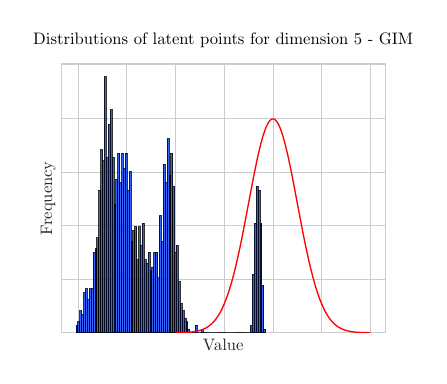
\begin{tikzpicture}[scale=0.6]

\definecolor{blue262255}{RGB}{2,62,255}
\definecolor{darkslategray38}{RGB}{38,38,38}
\definecolor{lightgray204}{RGB}{204,204,204}

\begin{axis}[
axis line style={lightgray204},
tick align=outside,
title={Distributions of latent points for dimension 5 - GIM},
x grid style={lightgray204},
xlabel=\textcolor{darkslategray38}{Value},
xmajorgrids,
xmajorticks=false,
xmin=-8.69137392044067, xmax=4.6043511390686,
xtick style={color=darkslategray38},
y grid style={lightgray204},
ylabel=\textcolor{darkslategray38}{Frequency},
ymajorgrids,
ymajorticks=false,
ymin=0, ymax=0.501859514232778,
ytick style={color=darkslategray38}
]
\draw[draw=black,fill=blue262255,opacity=0.8,line width=0.48pt] (axis cs:-8.08702278137207,0) rectangle (axis cs:-8.00916194915771,0.0136559575709611);
\draw[draw=black,fill=blue262255,opacity=0.8,line width=0.48pt] (axis cs:-8.0091609954834,0) rectangle (axis cs:-7.9313006401062,0.0204840618054195);
\draw[draw=black,fill=blue262255,opacity=0.8,line width=0.48pt] (axis cs:-7.9313006401062,0) rectangle (axis cs:-7.85343980789185,0.0409678727128832);
\draw[draw=black,fill=blue262255,opacity=0.8,line width=0.48pt] (axis cs:-7.85343980789185,0) rectangle (axis cs:-7.77557897567749,0.0341398939274027);
\draw[draw=black,fill=blue262255,opacity=0.8,line width=0.48pt] (axis cs:-7.77557897567749,0) rectangle (axis cs:-7.69771814346313,0.0751077666402859);
\draw[draw=black,fill=blue262255,opacity=0.8,line width=0.48pt] (axis cs:-7.69771766662598,0) rectangle (axis cs:-7.61985731124878,0.0819362472216781);
\draw[draw=black,fill=blue262255,opacity=0.8,line width=0.48pt] (axis cs:-7.61985778808594,0) rectangle (axis cs:-7.54199695587158,0.0614518090693249);
\draw[draw=black,fill=blue262255,opacity=0.8,line width=0.48pt] (axis cs:-7.54199695587158,0) rectangle (axis cs:-7.46413612365723,0.0819357454257665);
\draw[draw=black,fill=blue262255,opacity=0.8,line width=0.48pt] (axis cs:-7.46413612365723,0) rectangle (axis cs:-7.38627576828003,0.0819362472216781);
\draw[draw=black,fill=blue262255,opacity=0.8,line width=0.48pt] (axis cs:-7.38627576828003,0) rectangle (axis cs:-7.30841493606567,0.150215533280572);
\draw[draw=black,fill=blue262255,opacity=0.8,line width=0.48pt] (axis cs:-7.30841493606567,0) rectangle (axis cs:-7.23055410385132,0.157043512066052);
\draw[draw=black,fill=blue262255,opacity=0.8,line width=0.48pt] (axis cs:-7.23055410385132,0) rectangle (axis cs:-7.15269327163696,0.177527448422494);
\draw[draw=black,fill=blue262255,opacity=0.8,line width=0.48pt] (axis cs:-7.1526927947998,0) rectangle (axis cs:-7.07483243942261,0.266292803470454);
\draw[draw=black,fill=blue262255,opacity=0.8,line width=0.48pt] (axis cs:-7.07483291625977,0) rectangle (axis cs:-6.99697208404541,0.341398939274027);
\draw[draw=black,fill=blue262255,opacity=0.8,line width=0.48pt] (axis cs:-6.99697208404541,0) rectangle (axis cs:-6.91911125183105,0.320915002917585);
\draw[draw=black,fill=blue262255,opacity=0.8,line width=0.48pt] (axis cs:-6.91911125183105,0) rectangle (axis cs:-6.84125089645386,0.477961442126456);
\draw[draw=black,fill=blue262255,opacity=0.8,line width=0.48pt] (axis cs:-6.84125089645386,0) rectangle (axis cs:-6.7633900642395,0.327742981703066);
\draw[draw=black,fill=blue262255,opacity=0.8,line width=0.48pt] (axis cs:-6.7633900642395,0) rectangle (axis cs:-6.68552923202515,0.389194790772391);
\draw[draw=black,fill=blue262255,opacity=0.8,line width=0.48pt] (axis cs:-6.68552923202515,0) rectangle (axis cs:-6.60766839981079,0.416506705914313);
\draw[draw=black,fill=blue262255,opacity=0.8,line width=0.48pt] (axis cs:-6.60766792297363,0) rectangle (axis cs:-6.52980756759644,0.327744988886712);
\draw[draw=black,fill=blue262255,opacity=0.8,line width=0.48pt] (axis cs:-6.52980804443359,0) rectangle (axis cs:-6.45194721221924,0.238979257491819);
\draw[draw=black,fill=blue262255,opacity=0.8,line width=0.48pt] (axis cs:-6.45194721221924,0) rectangle (axis cs:-6.37408638000488,0.286775108990183);
\draw[draw=black,fill=blue262255,opacity=0.8,line width=0.48pt] (axis cs:-6.37408638000488,0) rectangle (axis cs:-6.29622602462769,0.334573009488519);
\draw[draw=black,fill=blue262255,opacity=0.8,line width=0.48pt] (axis cs:-6.29622602462769,0) rectangle (axis cs:-6.21836519241333,0.279947130204702);
\draw[draw=black,fill=blue262255,opacity=0.8,line width=0.48pt] (axis cs:-6.21836519241333,0) rectangle (axis cs:-6.14050436019897,0.334570960488546);
\draw[draw=black,fill=blue262255,opacity=0.8,line width=0.48pt] (axis cs:-6.14050436019897,0) rectangle (axis cs:-6.06264352798462,0.307259045346624);
\draw[draw=black,fill=blue262255,opacity=0.8,line width=0.48pt] (axis cs:-6.06264305114746,0) rectangle (axis cs:-5.98478269577026,0.334573009488519);
\draw[draw=black,fill=blue262255,opacity=0.8,line width=0.48pt] (axis cs:-5.98478317260742,0) rectangle (axis cs:-5.90692234039307,0.266291172633741);
\draw[draw=black,fill=blue262255,opacity=0.8,line width=0.48pt] (axis cs:-5.90692234039307,0) rectangle (axis cs:-5.82906150817871,0.300431066561144);
\draw[draw=black,fill=blue262255,opacity=0.8,line width=0.48pt] (axis cs:-5.82906150817871,0) rectangle (axis cs:-5.75120115280151,0.170700515045163);
\draw[draw=black,fill=blue262255,opacity=0.8,line width=0.48pt] (axis cs:-5.75120115280151,0) rectangle (axis cs:-5.67334032058716,0.191183405993455);
\draw[draw=black,fill=blue262255,opacity=0.8,line width=0.48pt] (axis cs:-5.67334032058716,0) rectangle (axis cs:-5.5954794883728,0.198011384778936);
\draw[draw=black,fill=blue262255,opacity=0.8,line width=0.48pt] (axis cs:-5.5954794883728,0) rectangle (axis cs:-5.51761865615845,0.136559575709611);
\draw[draw=black,fill=blue262255,opacity=0.8,line width=0.48pt] (axis cs:-5.51761817932129,0) rectangle (axis cs:-5.43975782394409,0.198012597452389);
\draw[draw=black,fill=blue262255,opacity=0.8,line width=0.48pt] (axis cs:-5.43975830078125,0) rectangle (axis cs:-5.36189746856689,0.163871490851533);
\draw[draw=black,fill=blue262255,opacity=0.8,line width=0.48pt] (axis cs:-5.36189746856689,0) rectangle (axis cs:-5.28403663635254,0.204839363564416);
\draw[draw=black,fill=blue262255,opacity=0.8,line width=0.48pt] (axis cs:-5.28403663635254,0) rectangle (axis cs:-5.20617628097534,0.13656041203613);
\draw[draw=black,fill=blue262255,opacity=0.8,line width=0.48pt] (axis cs:-5.20617628097534,0) rectangle (axis cs:-5.12831544876099,0.12973159692413);
\draw[draw=black,fill=blue262255,opacity=0.8,line width=0.48pt] (axis cs:-5.12831544876099,0) rectangle (axis cs:-5.05045461654663,0.150215533280572);
\draw[draw=black,fill=blue262255,opacity=0.8,line width=0.48pt] (axis cs:-5.05045461654663,0) rectangle (axis cs:-4.97259378433228,0.116075639353169);
\draw[draw=black,fill=blue262255,opacity=0.8,line width=0.48pt] (axis cs:-4.97259330749512,0) rectangle (axis cs:-4.89473295211792,0.122904370832517);
\draw[draw=black,fill=blue262255,opacity=0.8,line width=0.48pt] (axis cs:-4.89473342895508,0) rectangle (axis cs:-4.81687259674072,0.150215533280572);
\draw[draw=black,fill=blue262255,opacity=0.8,line width=0.48pt] (axis cs:-4.81687259674072,0) rectangle (axis cs:-4.73901176452637,0.150215533280572);
\draw[draw=black,fill=blue262255,opacity=0.8,line width=0.48pt] (axis cs:-4.73901176452637,0) rectangle (axis cs:-4.66115140914917,0.102420309027098);
\draw[draw=black,fill=blue262255,opacity=0.8,line width=0.48pt] (axis cs:-4.66115140914917,0) rectangle (axis cs:-4.58329057693481,0.218495321135377);
\draw[draw=black,fill=blue262255,opacity=0.8,line width=0.48pt] (axis cs:-4.58329057693481,0) rectangle (axis cs:-4.50542974472046,0.170699469637013);
\draw[draw=black,fill=blue262255,opacity=0.8,line width=0.48pt] (axis cs:-4.50542974472046,0) rectangle (axis cs:-4.4275689125061,0.314087024132105);
\draw[draw=black,fill=blue262255,opacity=0.8,line width=0.48pt] (axis cs:-4.42756843566895,0) rectangle (axis cs:-4.34970808029175,0.279948844674067);
\draw[draw=black,fill=blue262255,opacity=0.8,line width=0.48pt] (axis cs:-4.34970855712891,0) rectangle (axis cs:-4.27184772491455,0.361882875630469);
\draw[draw=black,fill=blue262255,opacity=0.8,line width=0.48pt] (axis cs:-4.27184772491455,0) rectangle (axis cs:-4.1939868927002,0.293603087775663);
\draw[draw=black,fill=blue262255,opacity=0.8,line width=0.48pt] (axis cs:-4.1939868927002,0) rectangle (axis cs:-4.116126537323,0.334573009488519);
\draw[draw=black,fill=blue262255,opacity=0.8,line width=0.48pt] (axis cs:-4.116126537323,0) rectangle (axis cs:-4.03826570510864,0.273119151419222);
\draw[draw=black,fill=blue262255,opacity=0.8,line width=0.48pt] (axis cs:-4.03826570510864,0) rectangle (axis cs:-3.96040487289429,0.150215533280572);
\draw[draw=black,fill=blue262255,opacity=0.8,line width=0.48pt] (axis cs:-3.96040487289429,0) rectangle (axis cs:-3.88254404067993,0.163871992645908);
\draw[draw=black,fill=blue262255,opacity=0.8,line width=0.48pt] (axis cs:-3.88254427909851,0) rectangle (axis cs:-3.80468344688416,0.0955917029967276);
\draw[draw=black,fill=blue262255,opacity=0.8,line width=0.48pt] (axis cs:-3.80468368530273,0) rectangle (axis cs:-3.72682285308838,0.054623997548636);
\draw[draw=black,fill=blue262255,opacity=0.8,line width=0.48pt] (axis cs:-3.72682285308838,0) rectangle (axis cs:-3.64896202087402,0.0409678727128832);
\draw[draw=black,fill=blue262255,opacity=0.8,line width=0.48pt] (axis cs:-3.64896202087402,0) rectangle (axis cs:-3.57110118865967,0.027311998774318);
\draw[draw=black,fill=blue262255,opacity=0.8,line width=0.48pt] (axis cs:-3.57110166549683,0) rectangle (axis cs:-3.49324083328247,0.0204839990807385);
\draw[draw=black,fill=blue262255,opacity=0.8,line width=0.48pt] (axis cs:-3.49324083328247,0) rectangle (axis cs:-3.41538000106812,0.00682797878548054);
\draw[draw=black,fill=blue262255,opacity=0.8,line width=0.48pt] (axis cs:-3.41538000106812,0) rectangle (axis cs:-3.33751916885376,0);
\draw[draw=black,fill=blue262255,opacity=0.8,line width=0.48pt] (axis cs:-3.33751940727234,0) rectangle (axis cs:-3.25965857505798,0);
\draw[draw=black,fill=blue262255,opacity=0.8,line width=0.48pt] (axis cs:-3.25965881347656,0) rectangle (axis cs:-3.18179798126221,0);
\draw[draw=black,fill=blue262255,opacity=0.8,line width=0.48pt] (axis cs:-3.18179798126221,0) rectangle (axis cs:-3.10393714904785,0.0136559575709611);
\draw[draw=black,fill=blue262255,opacity=0.8,line width=0.48pt] (axis cs:-3.10393714904785,0) rectangle (axis cs:-3.0260763168335,0);
\draw[draw=black,fill=blue262255,opacity=0.8,line width=0.48pt] (axis cs:-3.02607679367065,0) rectangle (axis cs:-2.9482159614563,0);
\draw[draw=black,fill=blue262255,opacity=0.8,line width=0.48pt] (axis cs:-2.9482159614563,0) rectangle (axis cs:-2.87035512924194,0.00682797878548054);
\draw[draw=black,fill=blue262255,opacity=0.8,line width=0.48pt] (axis cs:-2.87035512924194,0) rectangle (axis cs:-2.79249429702759,0);
\draw[draw=black,fill=blue262255,opacity=0.8,line width=0.48pt] (axis cs:-2.79249453544617,0) rectangle (axis cs:-2.71463370323181,0);
\draw[draw=black,fill=blue262255,opacity=0.8,line width=0.48pt] (axis cs:-2.71463394165039,0) rectangle (axis cs:-2.63677310943604,0);
\draw[draw=black,fill=blue262255,opacity=0.8,line width=0.48pt] (axis cs:-2.63677310943604,0) rectangle (axis cs:-2.55891227722168,0);
\draw[draw=black,fill=blue262255,opacity=0.8,line width=0.48pt] (axis cs:-2.55891227722168,0) rectangle (axis cs:-2.48105144500732,0);
\draw[draw=black,fill=blue262255,opacity=0.8,line width=0.48pt] (axis cs:-2.48105192184448,0) rectangle (axis cs:-2.40319108963013,0);
\draw[draw=black,fill=blue262255,opacity=0.8,line width=0.48pt] (axis cs:-2.40319108963013,0) rectangle (axis cs:-2.32533025741577,0);
\draw[draw=black,fill=blue262255,opacity=0.8,line width=0.48pt] (axis cs:-2.32533025741577,0) rectangle (axis cs:-2.24746942520142,0);
\draw[draw=black,fill=blue262255,opacity=0.8,line width=0.48pt] (axis cs:-2.24746966362,0) rectangle (axis cs:-2.16960883140564,0);
\draw[draw=black,fill=blue262255,opacity=0.8,line width=0.48pt] (axis cs:-2.16960906982422,0) rectangle (axis cs:-2.09174823760986,0);
\draw[draw=black,fill=blue262255,opacity=0.8,line width=0.48pt] (axis cs:-2.09174823760986,0) rectangle (axis cs:-2.01388740539551,0);
\draw[draw=black,fill=blue262255,opacity=0.8,line width=0.48pt] (axis cs:-2.01388740539551,0) rectangle (axis cs:-1.93602657318115,0);
\draw[draw=black,fill=blue262255,opacity=0.8,line width=0.48pt] (axis cs:-1.93602681159973,0) rectangle (axis cs:-1.85816597938538,0);
\draw[draw=black,fill=blue262255,opacity=0.8,line width=0.48pt] (axis cs:-1.85816621780396,0) rectangle (axis cs:-1.7803053855896,0);
\draw[draw=black,fill=blue262255,opacity=0.8,line width=0.48pt] (axis cs:-1.7803053855896,0) rectangle (axis cs:-1.70244455337524,0);
\draw[draw=black,fill=blue262255,opacity=0.8,line width=0.48pt] (axis cs:-1.70244479179382,0) rectangle (axis cs:-1.62458395957947,0);
\draw[draw=black,fill=blue262255,opacity=0.8,line width=0.48pt] (axis cs:-1.62458407878876,0) rectangle (axis cs:-1.5467232465744,0);
\draw[draw=black,fill=blue262255,opacity=0.8,line width=0.48pt] (axis cs:-1.54672336578369,0) rectangle (axis cs:-1.46886253356934,0);
\draw[draw=black,fill=blue262255,opacity=0.8,line width=0.48pt] (axis cs:-1.46886277198792,0) rectangle (axis cs:-1.39100193977356,0);
\draw[draw=black,fill=blue262255,opacity=0.8,line width=0.48pt] (axis cs:-1.39100193977356,0) rectangle (axis cs:-1.3131411075592,0);
\draw[draw=black,fill=blue262255,opacity=0.8,line width=0.48pt] (axis cs:-1.31314134597778,0) rectangle (axis cs:-1.23528051376343,0);
\draw[draw=black,fill=blue262255,opacity=0.8,line width=0.48pt] (axis cs:-1.23528051376343,0) rectangle (axis cs:-1.15741968154907,0);
\draw[draw=black,fill=blue262255,opacity=0.8,line width=0.48pt] (axis cs:-1.15741991996765,0) rectangle (axis cs:-1.0795590877533,0);
\draw[draw=black,fill=blue262255,opacity=0.8,line width=0.48pt] (axis cs:-1.07955920696259,0) rectangle (axis cs:-1.00169837474823,0);
\draw[draw=black,fill=blue262255,opacity=0.8,line width=0.48pt] (axis cs:-1.00169849395752,0) rectangle (axis cs:-0.923837661743164,0);
\draw[draw=black,fill=blue262255,opacity=0.8,line width=0.48pt] (axis cs:-0.923837780952454,0) rectangle (axis cs:-0.845976948738098,0.0136559889330855);
\draw[draw=black,fill=blue262255,opacity=0.8,line width=0.48pt] (axis cs:-0.845977127552032,0) rectangle (axis cs:-0.768116295337677,0.109247827832224);
\draw[draw=black,fill=blue262255,opacity=0.8,line width=0.48pt] (axis cs:-0.768116414546967,0) rectangle (axis cs:-0.690255582332611,0.20483967718542);
\draw[draw=black,fill=blue262255,opacity=0.8,line width=0.48pt] (axis cs:-0.690255701541901,0) rectangle (axis cs:-0.612394869327545,0.273119569580561);
\draw[draw=black,fill=blue262255,opacity=0.8,line width=0.48pt] (axis cs:-0.612395048141479,0) rectangle (axis cs:-0.534534215927124,0.266291784195168);
\draw[draw=black,fill=blue262255,opacity=0.8,line width=0.48pt] (axis cs:-0.534534335136414,0) rectangle (axis cs:-0.456673502922058,0.20483967718542);
\draw[draw=black,fill=blue262255,opacity=0.8,line width=0.48pt] (axis cs:-0.456673622131348,0) rectangle (axis cs:-0.378812789916992,0.0887638601136822);
\draw[draw=black,fill=blue262255,opacity=0.8,line width=0.48pt] (axis cs:-0.378812909126282,0) rectangle (axis cs:-0.300952076911926,0.00682799185302739);
\addplot [thick, red]
table {%
-4 0.000133830225764885
-3.99199199199199 0.000138182046410498
-3.98398398398398 0.000142666228042307
-3.97597597597598 0.000147286481503254
-3.96796796796797 0.000152046611333821
-3.95995995995996 0.000156950517814782
-3.95195195195195 0.00016200219904485
-3.94394394394394 0.00016720575305353
-3.93593593593594 0.000172565379949496
-3.92792792792793 0.00017808538410479
-3.91991991991992 0.000183770176375138
-3.91191191191191 0.000189624276356684
-3.9039039039039 0.000195652314679408
-3.8958958958959 0.000201859035337517
-3.88788788788789 0.000208249298057069
-3.87987987987988 0.000214828080701088
-3.87187187187187 0.000221600481712426
-3.86386386386386 0.0002285717225946
-3.85585585585586 0.000235747150430845
-3.84784784784785 0.000243132240441603
-3.83983983983984 0.000250732598580649
-3.83183183183183 0.000258553964170059
-3.82382382382382 0.000266602212574213
-3.81581581581582 0.000274883357912987
-3.80780780780781 0.000283403555814325
-3.7997997997998 0.000292169106206322
-3.79179179179179 0.000301186456148957
-3.78378378378378 0.0003104622027056
-3.77577577577578 0.000320003095854415
-3.76776776776777 0.000329816041439723
-3.75975975975976 0.000339908104163431
-3.75175175175175 0.00035028651061658
-3.74374374374374 0.000360958652351047
-3.73573573573574 0.000371932088991451
-3.72772772772773 0.000383214551387261
-3.71971971971972 0.000394813944805093
-3.71171171171171 0.000406738352161197
-3.7037037037037 0.000418996037294058
-3.6956956956957 0.00043159544827708
-3.68768768768769 0.00044454522077123
-3.67967967967968 0.000457854181417586
-3.67167167167167 0.000471531351269624
-3.66366366366366 0.000485585949265103
-3.65565565565566 0.000500027395737409
-3.64764764764765 0.000514865315966112
-3.63963963963964 0.000530109543766577
-3.63163163163163 0.000545770125118336
-3.62362362362362 0.000561857321831991
-3.61561561561562 0.00057838161525435
-3.60760760760761 0.000595353710011453
-3.5995995995996 0.000612784537789192
-3.59159159159159 0.000630685261151105
-3.58358358358358 0.000649067277392973
-3.57557557557558 0.000667942222433796
-3.56756756756757 0.000687321974742665
-3.55955955955956 0.000707218659301081
-3.55155155155155 0.000727644651600166
-3.54354354354354 0.000748612581672245
-3.53553553553554 0.000770135338156225
-3.52752752752753 0.000792226072396121
-3.51951951951952 0.00081489820257214
-3.51151151151151 0.000838165417863603
-3.5035035035035 0.000862041682643007
-3.4954954954955 0.000886541240700502
-3.48748748748749 0.00091167861949796
-3.47947947947948 0.000937468634451866
-3.47147147147147 0.000963926393244149
-3.46346346346346 0.000991067300160059
-3.45545545545546 0.0010189070604522
-3.44744744744745 0.00104746168472971
-3.43943943943944 0.0010767474933716
-3.43143143143143 0.00110678112096323
-3.42342342342342 0.00113757952075483
-3.41541541541542 0.00116915996914087
-3.40740740740741 0.00120154007015926
-3.3993993993994 0.00123473776000907
-3.39139139139139 0.00126877131158549
-3.38338338338338 0.00130365933903088
-3.37537537537538 0.00133942080230046
-3.36736736736737 0.00137607501174126
-3.35935935935936 0.001413641632683
-3.35135135135135 0.00145214069003938
-3.34334334334334 0.0014915925729182
-3.33533533533534 0.00153201803923895
-3.32732732732733 0.00157343822035606
-3.31931931931932 0.00161587462568624
-3.31131131131131 0.00165934914733831
-3.3033033033033 0.00170388406474362
-3.2952952952953 0.00174950204928538
-3.28728728728729 0.00179622616892505
-3.27927927927928 0.00184407989282385
-3.27127127127127 0.00189308709595757
-3.26326326326326 0.00194327206372255
-3.25525525525526 0.00199465949653091
-3.24724724724725 0.00204727451439301
-3.23923923923924 0.00210114266148476
-3.23123123123123 0.00215628991069791
-3.22322322322322 0.00221274266817093
-3.21521521521522 0.00227052777779815
-3.20720720720721 0.00232967252571501
-3.1991991991992 0.00239020464475689
-3.19119119119119 0.00245215231888918
-3.18318318318318 0.00251554418760605
-3.17517517517518 0.00258040935029545
-3.16716716716717 0.00264677737056774
-3.15915915915916 0.00271467828054534
-3.15115115115115 0.00278414258511061
-3.14314314314314 0.00285520126610952
-3.13513513513514 0.00292788578650791
-3.12712712712713 0.00300222809449793
-3.11911911911912 0.00307826062755151
-3.11111111111111 0.00315601631641804
-3.1031031031031 0.00323552858906328
-3.0950950950951 0.00331683137454643
-3.08708708708709 0.00339995910683238
-3.07907907907908 0.00348494672853595
-3.07107107107107 0.00357182969459489
-3.06306306306306 0.00366064397586864
-3.05505505505506 0.00375142606265932
-3.04704704704705 0.00384421296815189
-3.03903903903904 0.00393904223176991
-3.03103103103103 0.00403595192244368
-3.02302302302302 0.0041349806417872
-3.01501501501502 0.00423616752718052
-3.00700700700701 0.00433955225475399
-2.998998998999 0.00444517504227068
-2.99099099099099 0.00455307665190355
-2.98298298298298 0.00466329839290368
-2.97497497497497 0.00477588212415564
-2.96696696696697 0.00489087025661667
-2.95895895895896 0.00500830575563558
-2.95095095095095 0.00512823214314763
-2.94294294294294 0.00525069349974172
-2.93493493493493 0.00537573446659573
-2.92692692692693 0.00550340024727644
-2.91891891891892 0.00563373660939975
-2.91091091091091 0.0057667898861475
-2.9029029029029 0.00590260697763674
-2.89489489489489 0.00604123535213746
-2.88688688688689 0.00618272304713484
-2.87887887887888 0.00632711867023164
-2.87087087087087 0.00647447139988703
-2.86286286286286 0.00662483098598741
-2.85485485485485 0.0067782477502453
-2.84684684684685 0.0069347725864219
-2.83883883883884 0.00709445696036946
-2.83083083083083 0.00725735290988893
-2.82282282282282 0.00742351304439893
-2.81481481481481 0.00759299054441176
-2.80680680680681 0.0077658391608121
-2.7987987987988 0.00794211321393437
-2.79079079079079 0.00812186759243432
-2.78278278278278 0.00830515775195071
-2.77477477477477 0.00849203971355293
-2.76676676676677 0.00868257006197001
-2.75875875875876 0.00887680594359712
-2.75075075075075 0.00907480506427511
-2.74274274274274 0.00927662568683898
-2.73473473473473 0.00948232662843099
-2.72672672672673 0.00969196725757422
-2.71871871871872 0.00990560749100246
-2.71071071071071 0.0101233077902421
-2.7027027027027 0.0103451291579421
-2.69469469469469 0.0105711331339476
-2.68668668668669 0.0108013817911136
-2.67867867867868 0.011035937730854
-2.67067067067067 0.0112748640784219
-2.66266266266266 0.0115182244779185
-2.65465465465465 0.0117660830870247
-2.64664664664665 0.0120185045714526
-2.63863863863864 0.0122755540991133
-2.63063063063063 0.0125372973339956
-2.62262262262262 0.0128038004297541
-2.61461461461461 0.0130751300230007
-2.60660660660661 0.0133513532262973
-2.5985985985986 0.0136325376208454
-2.59059059059059 0.0139187512488692
-2.58258258258258 0.014210062605689
-2.57457457457457 0.0145065406314803
-2.56656656656657 0.0148082547027168
-2.55855855855856 0.0151152746232934
-2.55055055055055 0.0154276706153247
-2.54254254254254 0.0157455133096184
-2.53453453453453 0.0160688737358178
-2.52652652652653 0.016397823312213
-2.51851851851852 0.0167324338352151
-2.51051051051051 0.0170727774684938
-2.5025025025025 0.0174189267317727
-2.49449449449449 0.0177709544892815
-2.48648648648649 0.0181289339378627
-2.47847847847848 0.0184929385947284
-2.47047047047047 0.0188630422848682
-2.46246246246246 0.0192393191281025
-2.45445445445445 0.0196218435257817
-2.44644644644645 0.0200106901471285
-2.43843843843844 0.020405933915221
-2.43043043043043 0.0208076499926159
-2.42242242242242 0.0212159137666093
-2.41441441441441 0.0216308008341344
-2.40640640640641 0.0220523869862944
-2.3983983983984 0.0224807481925294
-2.39039039039039 0.022915960584417
-2.38238238238238 0.0233581004391047
-2.37437437437437 0.023807244162374
-2.36636636636637 0.0242634682713357
-2.35835835835836 0.0247268493767558
-2.35035035035035 0.0251974641650118
-2.34234234234234 0.0256753893796796
-2.33433433433433 0.0261607018027501
-2.32632632632633 0.0266534782354775
-2.31831831831832 0.0271537954788581
-2.31031031031031 0.0276617303137407
-2.3023023023023 0.0281773594805703
-2.29429429429429 0.0287007596587648
-2.28628628628629 0.0292320074457259
-2.27827827827828 0.029771179335487
-2.27027027027027 0.0303183516969979
-2.26226226226226 0.0308736007520491
-2.25425425425425 0.0314370025528369
-2.24624624624625 0.0320086329591723
-2.23823823823824 0.0325885676153351
-2.23023023023023 0.0331768819265761
-2.22222222222222 0.0337736510352706
-2.21421421421421 0.0343789497967251
-2.20620620620621 0.0349928527546413
-2.1981981981982 0.0356154341162401
-2.19019019019019 0.0362467677270497
-2.18218218218218 0.0368869270453615
-2.17417417417417 0.0375359851163567
-2.16616616616617 0.03819401454591
-2.15815815815816 0.0388610874740724
-2.15015015015015 0.03953727554824
-2.14214214214214 0.0402226498960119
-2.13413413413413 0.0409172810977437
-2.12612612612613 0.0416212391588003
-2.11811811811812 0.0423345934815158
-2.11011011011011 0.0430574128368641
-2.1021021021021 0.043789765335848
-2.09409409409409 0.0445317184006117
-2.08608608608609 0.0452833387352837
-2.07807807807808 0.0460446922965577
-2.07007007007007 0.0468158442640166
-2.06206206206206 0.0475968590102091
-2.05405405405405 0.0483878000704834
-2.04604604604605 0.0491887301125894
-2.03803803803804 0.0499997109060533
-2.03003003003003 0.0508208032913361
-2.02202202202202 0.0516520671487823
-2.01401401401401 0.0524935613673682
-2.00600600600601 0.053345343813258
-1.997997997998 0.0542074712981785
-1.98998998998999 0.0550799995476186
-1.98198198198198 0.0559629831688668
-1.97397397397397 0.0568564756188931
-1.96596596596597 0.0577605291720876
-1.95795795795796 0.0586751948878651
-1.94994994994995 0.0596005225781457
-1.94194194194194 0.0605365607747232
-1.93393393393393 0.0614833566965309
-1.92592592592593 0.062440956216817
-1.91791791791792 0.06340940383024
-1.90990990990991 0.0643887426198963
-1.9019019019019 0.0653790142242912
-1.89389389389389 0.0663802588042656
-1.88588588588589 0.0673925150098903
-1.87787787787788 0.0684158199473405
-1.86986986986987 0.0694502091457625
-1.86186186186186 0.0704957165241465
-1.85385385385385 0.0715523743582165
-1.84584584584585 0.0726202132473521
-1.83783783783784 0.0736992620815557
-1.82982982982983 0.0747895480084762
-1.82182182182182 0.0758910964005057
-1.81381381381381 0.0770039308219614
-1.80580580580581 0.0781280729963669
-1.7977977977978 0.0792635427738473
-1.78978978978979 0.0804103580986525
-1.78178178178178 0.0815685349768227
-1.77377377377377 0.0827380874440109
-1.76576576576577 0.0839190275334777
-1.75775775775776 0.0851113652442723
-1.74974974974975 0.086315108509615
-1.74174174174174 0.0875302631654975
-1.73373373373373 0.0887568329195139
-1.72572572572573 0.0899948193199405
-1.71771771771772 0.0912442217250772
-1.70970970970971 0.0925050372728685
-1.7017017017017 0.0937772608508177
-1.69369369369369 0.0950608850662112
-1.68568568568569 0.0963559002166691
-1.67767767767768 0.0976622942610365
-1.66966966966967 0.0989800527906321
-1.66166166166166 0.100309159000872
-1.65365365365365 0.10164959366328
-1.64564564564565 0.103001335097907
-1.63763763763764 0.10436435914617
-1.62962962962963 0.105738639144131
-1.62162162162162 0.107124145896225
-1.61361361361361 0.108520847649465
-1.60560560560561 0.10992871006813
-1.5975975975976 0.111347696208955
-1.58958958958959 0.112777766496842
-1.58158158158158 0.114218878701105
-1.57357357357357 0.115670987912262
-1.56556556556557 0.117134046519405
-1.55755755755756 0.11860800418814
-1.54954954954955 0.120092807839133
-1.54154154154154 0.121588401627275
-1.53353353353353 0.123094726921466
-1.52552552552553 0.124611722285057
-1.51751751751752 0.12613932345695
-1.50950950950951 0.127677463333369
-1.5015015015015 0.129226071950339
-1.49349349349349 0.130785076466857
-1.48548548548549 0.132354401148798
-1.47747747747748 0.133933967353555
-1.46946946946947 0.13552369351543
-1.46146146146146 0.137123495131801
-1.45345345345345 0.13873328475006
-1.44544544544545 0.140352971955359
-1.43743743743744 0.141982463359159
-1.42942942942943 0.143621662588612
-1.42142142142142 0.14527047027677
-1.41341341341341 0.146928784053658
-1.40540540540541 0.148596498538208
-1.3973973973974 0.150273505331067
-1.38938938938939 0.151959693008306
-1.38138138138138 0.153654947116025
-1.37337337337337 0.155359150165875
-1.36536536536537 0.157072181631514
-1.35735735735736 0.158793917945997
-1.34934934934935 0.160524232500121
-1.34134134134134 0.16226299564173
-1.33333333333333 0.164010074675994
-1.32532532532533 0.165765333866673
-1.31731731731732 0.167528634438376
-1.30930930930931 0.169299834579821
-1.3013013013013 0.17107878944811
-1.29329329329329 0.172865351174024
-1.28528528528529 0.174659368868355
-1.27727727727728 0.176460688629273
-1.26926926926927 0.178269153550739
-1.26126126126126 0.180084603731981
-1.25325325325325 0.181906876288021
-1.24524524524525 0.183735805361283
-1.23723723723724 0.185571222134271
-1.22922922922923 0.187412954843324
-1.22122122122122 0.18926082879347
-1.21321321321321 0.191114666374361
-1.20520520520521 0.192974287077311
-1.1971971971972 0.194839507513435
-1.18918918918919 0.19671014143289
-1.18118118118118 0.198585999745227
-1.17317317317317 0.200466890540856
-1.16516516516517 0.202352619113618
-1.15715715715716 0.204242987984477
-1.14914914914915 0.206137796926331
-1.14114114114114 0.208036842989938
-1.13313313313313 0.209939920530956
-1.12512512512513 0.21184682123811
-1.11711711711712 0.21375733416247
-1.10910910910911 0.215671245747847
-1.1011011011011 0.217588339862305
-1.09309309309309 0.219508397830784
-1.08508508508509 0.221431198468836
-1.07707707707708 0.223356518117463
-1.06906906906907 0.225284130679063
-1.06106106106106 0.22721380765447
-1.05305305305305 0.229145318181096
-1.04504504504505 0.231078429072154
-1.03703703703704 0.233012904856966
-1.02902902902903 0.234948507822352
-1.02102102102102 0.236884998055083
-1.01301301301301 0.238822133485401
-1.00500500500501 0.24075966993159
-0.996996996996997 0.242697361145593
-0.988988988988989 0.244634958859672
-0.980980980980981 0.246572212834085
-0.972972972972973 0.248508870905785
-0.964964964964965 0.250444679038131
-0.956956956956957 0.252379381371581
-0.948948948948949 0.254312720275385
-0.940940940940941 0.256244436400228
-0.932932932932933 0.258174268731856
-0.924924924924925 0.260101954645624
-0.916916916916917 0.262027229961987
-0.908908908908909 0.263949829002911
-0.900900900900901 0.265869484649172
-0.892892892892893 0.267785928398552
-0.884884884884885 0.269698890424904
-0.876876876876877 0.271608099638066
-0.868868868868869 0.273513283744617
-0.860860860860861 0.275414169309444
-0.852852852852853 0.277310481818125
-0.844844844844845 0.279201945740075
-0.836836836836837 0.281088284592474
-0.828828828828829 0.28296922100493
-0.820820820820821 0.284844476784867
-0.812812812812813 0.286713772983616
-0.804804804804805 0.288576829963198
-0.796796796796797 0.290433367463758
-0.788788788788789 0.292283104671645
-0.780780780780781 0.294125760288111
-0.772772772772773 0.295961052598604
-0.764764764764765 0.29778869954263
-0.756756756756757 0.299608418784177
-0.748748748748749 0.301419927782648
-0.740740740740741 0.303222943864308
-0.732732732732733 0.305017184294205
-0.724724724724725 0.306802366348536
-0.716716716716717 0.308578207387456
-0.708708708708709 0.310344424928268
-0.700700700700701 0.312100736719007
-0.692692692692693 0.313846860812361
-0.684684684684685 0.31558251563992
-0.676676676676677 0.317307420086723
-0.668668668668669 0.319021293566066
-0.660660660660661 0.320723856094559
-0.652652652652653 0.322414828367396
-0.644644644644645 0.324093931833804
-0.636636636636636 0.325760888772662
-0.628628628628629 0.327415422368237
-0.620620620620621 0.329057256786028
-0.612612612612613 0.330686117248681
-0.604604604604605 0.33230173011195
-0.596596596596596 0.333903822940662
-0.588588588588589 0.335492124584683
-0.580580580580581 0.337066365254824
-0.572572572572573 0.338626276598684
-0.564564564564565 0.340171591776383
-0.556556556556556 0.341702045536168
-0.548548548548549 0.343217374289848
-0.54054054054054 0.344717316188045
-0.532532532532533 0.346201611195215
-0.524524524524525 0.347670001164422
-0.516516516516516 0.349122229911825
-0.508508508508509 0.350558043290856
-0.5005005005005 0.351977189266054
-0.492492492492492 0.353379417986526
-0.484484484484485 0.354764481859011
-0.476476476476476 0.356132135620502
-0.468468468468469 0.357482136410418
-0.46046046046046 0.358814243842273
-0.452452452452452 0.360128220074839
-0.444444444444445 0.361423829882744
-0.436436436436436 0.362700840726495
-0.428428428428429 0.363959022821904
-0.42042042042042 0.365198149208855
-0.412412412412412 0.366417995819425
-0.404404404404405 0.3676183415453
-0.396396396396396 0.368798968304465
-0.388388388388389 0.369959661107154
-0.38038038038038 0.37110020812101
-0.372372372372372 0.372220400735444
-0.364364364364365 0.373320033625156
-0.356356356356356 0.374398904812801
-0.348348348348348 0.375456815730761
-0.34034034034034 0.376493571282005
-0.332332332332332 0.377508979900006
-0.324324324324325 0.378502853607702
-0.316316316316316 0.379475008075448
-0.308308308308308 0.380425262677969
-0.3003003003003 0.38135344055026
-0.292292292292292 0.382259368642425
-0.284284284284285 0.38314287777343
-0.276276276276276 0.384003802683735
-0.268268268268268 0.3848419820868
-0.26026026026026 0.385657258719425
-0.252252252252252 0.386449479390916
-0.244244244244244 0.387218495031049
-0.236236236236236 0.387964160736805
-0.228228228228228 0.38868633581787
-0.22022022022022 0.389384883840873
-0.212212212212212 0.390059672672329
-0.204204204204204 0.390710574520297
-0.196196196196196 0.391337465974705
-0.188188188188188 0.39194022804635
-0.18018018018018 0.392518746204527
-0.172172172172172 0.393072910413305
-0.164164164164164 0.393602615166401
-0.156156156156156 0.394107759520658
-0.148148148148148 0.394588247128102
-0.14014014014014 0.395043986266573
-0.132132132132132 0.3954748898689
-0.124124124124124 0.395880875550626
-0.116116116116116 0.396261865636259
-0.108108108108108 0.396617787184037
-0.1001001001001 0.396948572009207
-0.0920920920920922 0.397254156705792
-0.084084084084084 0.397534482666846
-0.0760760760760761 0.39778949610319
-0.0680680680680683 0.39801914806061
-0.06006006006006 0.398223394435522
-0.0520520520520522 0.398402195989086
-0.0440440440440439 0.398555518359772
-0.0360360360360361 0.398683332074364
-0.0280280280280278 0.398785612557403
-0.02002002002002 0.398862340139061
-0.0120120120120122 0.398913500061449
-0.00400400400400391 0.398939082483343
0.00400400400400436 0.398939082483343
0.0120120120120122 0.398913500061449
0.02002002002002 0.398862340139061
0.0280280280280278 0.398785612557403
0.0360360360360357 0.398683332074364
0.0440440440440444 0.398555518359772
0.0520520520520522 0.398402195989086
0.06006006006006 0.398223394435522
0.0680680680680679 0.39801914806061
0.0760760760760757 0.39778949610319
0.0840840840840844 0.397534482666846
0.0920920920920922 0.397254156705792
0.1001001001001 0.396948572009207
0.108108108108108 0.396617787184037
0.116116116116116 0.396261865636259
0.124124124124124 0.395880875550626
0.132132132132132 0.3954748898689
0.14014014014014 0.395043986266573
0.148148148148148 0.394588247128102
0.156156156156156 0.394107759520658
0.164164164164164 0.393602615166401
0.172172172172172 0.393072910413305
0.18018018018018 0.392518746204527
0.188188188188188 0.39194022804635
0.196196196196196 0.391337465974705
0.204204204204204 0.390710574520297
0.212212212212212 0.390059672672329
0.22022022022022 0.389384883840873
0.228228228228228 0.388686335817871
0.236236236236236 0.387964160736805
0.244244244244245 0.387218495031049
0.252252252252252 0.386449479390916
0.26026026026026 0.385657258719425
0.268268268268268 0.3848419820868
0.276276276276276 0.384003802683735
0.284284284284285 0.38314287777343
0.292292292292292 0.382259368642425
0.3003003003003 0.38135344055026
0.308308308308308 0.380425262677969
0.316316316316316 0.379475008075448
0.324324324324325 0.378502853607702
0.332332332332332 0.377508979900006
0.34034034034034 0.376493571282005
0.348348348348348 0.375456815730762
0.356356356356356 0.374398904812801
0.364364364364365 0.373320033625156
0.372372372372372 0.372220400735444
0.38038038038038 0.37110020812101
0.388388388388388 0.369959661107154
0.396396396396397 0.368798968304465
0.404404404404405 0.3676183415453
0.412412412412412 0.366417995819425
0.42042042042042 0.365198149208855
0.428428428428428 0.363959022821904
0.436436436436437 0.362700840726495
0.444444444444445 0.361423829882744
0.452452452452452 0.360128220074839
0.46046046046046 0.358814243842273
0.468468468468468 0.357482136410418
0.476476476476477 0.356132135620502
0.484484484484485 0.354764481859011
0.492492492492492 0.353379417986526
0.5005005005005 0.351977189266054
0.508508508508508 0.350558043290856
0.516516516516517 0.349122229911825
0.524524524524525 0.347670001164422
0.532532532532533 0.346201611195215
0.54054054054054 0.344717316188045
0.548548548548548 0.343217374289848
0.556556556556557 0.341702045536168
0.564564564564565 0.340171591776383
0.572572572572573 0.338626276598684
0.58058058058058 0.337066365254824
0.588588588588588 0.335492124584683
0.596596596596597 0.333903822940662
0.604604604604605 0.33230173011195
0.612612612612613 0.330686117248681
0.62062062062062 0.329057256786028
0.628628628628628 0.327415422368237
0.636636636636637 0.325760888772662
0.644644644644645 0.324093931833804
0.652652652652653 0.322414828367396
0.66066066066066 0.32072385609456
0.668668668668668 0.319021293566066
0.676676676676677 0.317307420086723
0.684684684684685 0.31558251563992
0.692692692692693 0.313846860812361
0.7007007007007 0.312100736719007
0.708708708708708 0.310344424928268
0.716716716716717 0.308578207387456
0.724724724724725 0.306802366348536
0.732732732732733 0.305017184294205
0.74074074074074 0.303222943864308
0.748748748748748 0.301419927782648
0.756756756756757 0.299608418784177
0.764764764764765 0.29778869954263
0.772772772772773 0.295961052598604
0.780780780780781 0.294125760288111
0.788788788788788 0.292283104671645
0.796796796796797 0.290433367463758
0.804804804804805 0.288576829963198
0.812812812812813 0.286713772983616
0.820820820820821 0.284844476784867
0.828828828828828 0.282969221004931
0.836836836836837 0.281088284592474
0.844844844844845 0.279201945740075
0.852852852852853 0.277310481818125
0.860860860860861 0.275414169309444
0.868868868868869 0.273513283744617
0.876876876876877 0.271608099638066
0.884884884884885 0.269698890424904
0.892892892892893 0.267785928398552
0.900900900900901 0.265869484649172
0.908908908908909 0.263949829002911
0.916916916916917 0.262027229961987
0.924924924924925 0.260101954645624
0.932932932932933 0.258174268731856
0.940940940940941 0.256244436400228
0.948948948948949 0.254312720275384
0.956956956956957 0.252379381371581
0.964964964964965 0.250444679038131
0.972972972972973 0.248508870905785
0.980980980980981 0.246572212834085
0.988988988988989 0.244634958859672
0.996996996996997 0.242697361145593
1.00500500500501 0.24075966993159
1.01301301301301 0.238822133485401
1.02102102102102 0.236884998055083
1.02902902902903 0.234948507822352
1.03703703703704 0.233012904856966
1.04504504504505 0.231078429072154
1.05305305305305 0.229145318181096
1.06106106106106 0.22721380765447
1.06906906906907 0.225284130679062
1.07707707707708 0.223356518117463
1.08508508508509 0.221431198468836
1.09309309309309 0.219508397830784
1.1011011011011 0.217588339862305
1.10910910910911 0.215671245747847
1.11711711711712 0.21375733416247
1.12512512512513 0.21184682123811
1.13313313313313 0.209939920530956
1.14114114114114 0.208036842989938
1.14914914914915 0.206137796926331
1.15715715715716 0.204242987984477
1.16516516516517 0.202352619113618
1.17317317317317 0.200466890540856
1.18118118118118 0.198585999745228
1.18918918918919 0.19671014143289
1.1971971971972 0.194839507513435
1.20520520520521 0.192974287077311
1.21321321321321 0.191114666374361
1.22122122122122 0.18926082879347
1.22922922922923 0.187412954843324
1.23723723723724 0.185571222134271
1.24524524524525 0.183735805361283
1.25325325325325 0.181906876288021
1.26126126126126 0.180084603731981
1.26926926926927 0.178269153550739
1.27727727727728 0.176460688629273
1.28528528528529 0.174659368868355
1.29329329329329 0.172865351174024
1.3013013013013 0.17107878944811
1.30930930930931 0.169299834579821
1.31731731731732 0.167528634438376
1.32532532532533 0.165765333866673
1.33333333333333 0.164010074675994
1.34134134134134 0.16226299564173
1.34934934934935 0.160524232500121
1.35735735735736 0.158793917945997
1.36536536536537 0.157072181631514
1.37337337337337 0.155359150165875
1.38138138138138 0.153654947116025
1.38938938938939 0.151959693008306
1.3973973973974 0.150273505331067
1.40540540540541 0.148596498538208
1.41341341341341 0.146928784053658
1.42142142142142 0.14527047027677
1.42942942942943 0.143621662588612
1.43743743743744 0.141982463359159
1.44544544544545 0.140352971955359
1.45345345345345 0.13873328475006
1.46146146146146 0.137123495131801
1.46946946946947 0.13552369351543
1.47747747747748 0.133933967353555
1.48548548548549 0.132354401148798
1.49349349349349 0.130785076466857
1.5015015015015 0.129226071950339
1.50950950950951 0.127677463333369
1.51751751751752 0.12613932345695
1.52552552552553 0.124611722285057
1.53353353353353 0.123094726921466
1.54154154154154 0.121588401627275
1.54954954954955 0.120092807839133
1.55755755755756 0.11860800418814
1.56556556556557 0.117134046519405
1.57357357357357 0.115670987912262
1.58158158158158 0.114218878701105
1.58958958958959 0.112777766496842
1.5975975975976 0.111347696208955
1.60560560560561 0.10992871006813
1.61361361361361 0.108520847649465
1.62162162162162 0.107124145896225
1.62962962962963 0.105738639144131
1.63763763763764 0.10436435914617
1.64564564564565 0.103001335097907
1.65365365365365 0.10164959366328
1.66166166166166 0.100309159000872
1.66966966966967 0.0989800527906321
1.67767767767768 0.0976622942610365
1.68568568568569 0.0963559002166692
1.69369369369369 0.0950608850662112
1.7017017017017 0.0937772608508176
1.70970970970971 0.0925050372728685
1.71771771771772 0.0912442217250772
1.72572572572573 0.0899948193199405
1.73373373373373 0.088756832919514
1.74174174174174 0.0875302631654974
1.74974974974975 0.086315108509615
1.75775775775776 0.0851113652442723
1.76576576576577 0.0839190275334778
1.77377377377377 0.082738087444011
1.78178178178178 0.0815685349768226
1.78978978978979 0.0804103580986525
1.7977977977978 0.0792635427738473
1.80580580580581 0.0781280729963669
1.81381381381381 0.0770039308219615
1.82182182182182 0.0758910964005057
1.82982982982983 0.0747895480084762
1.83783783783784 0.0736992620815557
1.84584584584585 0.0726202132473522
1.85385385385385 0.0715523743582165
1.86186186186186 0.0704957165241465
1.86986986986987 0.0694502091457625
1.87787787787788 0.0684158199473405
1.88588588588589 0.0673925150098903
1.89389389389389 0.0663802588042655
1.9019019019019 0.0653790142242912
1.90990990990991 0.0643887426198963
1.91791791791792 0.06340940383024
1.92592592592593 0.0624409562168171
1.93393393393393 0.0614833566965309
1.94194194194194 0.0605365607747232
1.94994994994995 0.0596005225781457
1.95795795795796 0.0586751948878651
1.96596596596597 0.0577605291720876
1.97397397397397 0.056856475618893
1.98198198198198 0.0559629831688668
1.98998998998999 0.0550799995476186
1.997997997998 0.0542074712981785
2.00600600600601 0.0533453438132581
2.01401401401401 0.0524935613673681
2.02202202202202 0.0516520671487823
2.03003003003003 0.0508208032913361
2.03803803803804 0.0499997109060533
2.04604604604605 0.0491887301125894
2.05405405405405 0.0483878000704834
2.06206206206206 0.0475968590102091
2.07007007007007 0.0468158442640166
2.07807807807808 0.0460446922965577
2.08608608608609 0.0452833387352837
2.09409409409409 0.0445317184006117
2.1021021021021 0.043789765335848
2.11011011011011 0.0430574128368641
2.11811811811812 0.0423345934815158
2.12612612612613 0.0416212391588004
2.13413413413413 0.0409172810977437
2.14214214214214 0.0402226498960119
2.15015015015015 0.03953727554824
2.15815815815816 0.0388610874740724
2.16616616616617 0.03819401454591
2.17417417417417 0.0375359851163567
2.18218218218218 0.0368869270453615
2.19019019019019 0.0362467677270497
2.1981981981982 0.0356154341162401
2.20620620620621 0.0349928527546413
2.21421421421421 0.0343789497967251
2.22222222222222 0.0337736510352706
2.23023023023023 0.0331768819265761
2.23823823823824 0.0325885676153351
2.24624624624625 0.0320086329591724
2.25425425425425 0.0314370025528369
2.26226226226226 0.0308736007520491
2.27027027027027 0.0303183516969979
2.27827827827828 0.029771179335487
2.28628628628629 0.0292320074457259
2.29429429429429 0.0287007596587648
2.3023023023023 0.0281773594805703
2.31031031031031 0.0276617303137407
2.31831831831832 0.0271537954788581
2.32632632632633 0.0266534782354776
2.33433433433433 0.0261607018027501
2.34234234234234 0.0256753893796796
2.35035035035035 0.0251974641650118
2.35835835835836 0.0247268493767558
2.36636636636637 0.0242634682713357
2.37437437437437 0.023807244162374
2.38238238238238 0.0233581004391047
2.39039039039039 0.022915960584417
2.3983983983984 0.0224807481925294
2.40640640640641 0.0220523869862944
2.41441441441441 0.0216308008341344
2.42242242242242 0.0212159137666093
2.43043043043043 0.0208076499926159
2.43843843843844 0.020405933915221
2.44644644644645 0.0200106901471285
2.45445445445445 0.0196218435257817
2.46246246246246 0.0192393191281025
2.47047047047047 0.0188630422848682
2.47847847847848 0.0184929385947284
2.48648648648649 0.0181289339378626
2.49449449449449 0.0177709544892815
2.5025025025025 0.0174189267317727
2.51051051051051 0.0170727774684938
2.51851851851852 0.0167324338352152
2.52652652652653 0.016397823312213
2.53453453453453 0.0160688737358178
2.54254254254254 0.0157455133096184
2.55055055055055 0.0154276706153247
2.55855855855856 0.0151152746232934
2.56656656656657 0.0148082547027168
2.57457457457457 0.0145065406314803
2.58258258258258 0.014210062605689
2.59059059059059 0.0139187512488692
2.5985985985986 0.0136325376208454
2.60660660660661 0.0133513532262973
2.61461461461461 0.0130751300230007
2.62262262262262 0.0128038004297541
2.63063063063063 0.0125372973339956
2.63863863863864 0.0122755540991133
2.64664664664665 0.0120185045714526
2.65465465465465 0.0117660830870247
2.66266266266266 0.0115182244779185
2.67067067067067 0.0112748640784219
2.67867867867868 0.011035937730854
2.68668668668669 0.0108013817911136
2.69469469469469 0.0105711331339476
2.7027027027027 0.0103451291579421
2.71071071071071 0.0101233077902421
2.71871871871872 0.00990560749100247
2.72672672672673 0.00969196725757422
2.73473473473473 0.00948232662843099
2.74274274274274 0.00927662568683898
2.75075075075075 0.00907480506427511
2.75875875875876 0.00887680594359712
2.76676676676677 0.00868257006197001
2.77477477477477 0.00849203971355293
2.78278278278278 0.00830515775195071
2.79079079079079 0.00812186759243432
2.7987987987988 0.00794211321393438
2.80680680680681 0.0077658391608121
2.81481481481481 0.00759299054441176
2.82282282282282 0.00742351304439893
2.83083083083083 0.00725735290988893
2.83883883883884 0.00709445696036947
2.84684684684685 0.0069347725864219
2.85485485485485 0.0067782477502453
2.86286286286286 0.00662483098598741
2.87087087087087 0.00647447139988703
2.87887887887888 0.00632711867023165
2.88688688688689 0.00618272304713484
2.89489489489489 0.00604123535213746
2.9029029029029 0.00590260697763674
2.91091091091091 0.0057667898861475
2.91891891891892 0.00563373660939975
2.92692692692693 0.00550340024727644
2.93493493493493 0.00537573446659573
2.94294294294294 0.00525069349974172
2.95095095095095 0.00512823214314764
2.95895895895896 0.00500830575563558
2.96696696696697 0.00489087025661667
2.97497497497497 0.00477588212415564
2.98298298298298 0.00466329839290368
2.99099099099099 0.00455307665190356
2.998998998999 0.00444517504227067
3.00700700700701 0.00433955225475399
3.01501501501502 0.00423616752718052
3.02302302302302 0.0041349806417872
3.03103103103103 0.00403595192244368
3.03903903903904 0.00393904223176991
3.04704704704705 0.00384421296815189
3.05505505505506 0.00375142606265932
3.06306306306306 0.00366064397586864
3.07107107107107 0.00357182969459489
3.07907907907908 0.00348494672853594
3.08708708708709 0.00339995910683238
3.0950950950951 0.00331683137454643
3.1031031031031 0.00323552858906328
3.11111111111111 0.00315601631641805
3.11911911911912 0.00307826062755151
3.12712712712713 0.00300222809449793
3.13513513513514 0.00292788578650791
3.14314314314314 0.00285520126610952
3.15115115115115 0.00278414258511062
3.15915915915916 0.00271467828054533
3.16716716716717 0.00264677737056774
3.17517517517518 0.00258040935029545
3.18318318318318 0.00251554418760605
3.19119119119119 0.00245215231888919
3.1991991991992 0.00239020464475689
3.20720720720721 0.00232967252571501
3.21521521521522 0.00227052777779815
3.22322322322322 0.00221274266817093
3.23123123123123 0.00215628991069792
3.23923923923924 0.00210114266148476
3.24724724724725 0.00204727451439301
3.25525525525526 0.00199465949653091
3.26326326326326 0.00194327206372255
3.27127127127127 0.00189308709595757
3.27927927927928 0.00184407989282385
3.28728728728729 0.00179622616892505
3.2952952952953 0.00174950204928538
3.3033033033033 0.00170388406474362
3.31131131131131 0.00165934914733832
3.31931931931932 0.00161587462568624
3.32732732732733 0.00157343822035606
3.33533533533534 0.00153201803923895
3.34334334334334 0.0014915925729182
3.35135135135135 0.00145214069003938
3.35935935935936 0.001413641632683
3.36736736736737 0.00137607501174126
3.37537537537538 0.00133942080230046
3.38338338338338 0.00130365933903089
3.39139139139139 0.00126877131158549
3.3993993993994 0.00123473776000907
3.40740740740741 0.00120154007015926
3.41541541541542 0.00116915996914087
3.42342342342342 0.00113757952075483
3.43143143143143 0.00110678112096324
3.43943943943944 0.0010767474933716
3.44744744744745 0.00104746168472971
3.45545545545546 0.0010189070604522
3.46346346346346 0.000991067300160061
3.47147147147147 0.000963926393244148
3.47947947947948 0.000937468634451866
3.48748748748749 0.00091167861949796
3.4954954954955 0.000886541240700502
3.5035035035035 0.000862041682643008
3.51151151151151 0.000838165417863601
3.51951951951952 0.00081489820257214
3.52752752752753 0.000792226072396121
3.53553553553554 0.000770135338156225
3.54354354354354 0.000748612581672247
3.55155155155155 0.000727644651600165
3.55955955955956 0.000707218659301081
3.56756756756757 0.000687321974742665
3.57557557557558 0.000667942222433796
3.58358358358358 0.000649067277392974
3.59159159159159 0.000630685261151104
3.5995995995996 0.000612784537789192
3.60760760760761 0.000595353710011453
3.61561561561562 0.00057838161525435
3.62362362362362 0.000561857321831992
3.63163163163163 0.000545770125118335
3.63963963963964 0.000530109543766577
3.64764764764765 0.000514865315966112
3.65565565565566 0.000500027395737409
3.66366366366366 0.000485585949265104
3.67167167167167 0.000471531351269623
3.67967967967968 0.000457854181417586
3.68768768768769 0.00044454522077123
3.6956956956957 0.00043159544827708
3.7037037037037 0.000418996037294059
3.71171171171171 0.000406738352161196
3.71971971971972 0.000394813944805093
3.72772772772773 0.000383214551387261
3.73573573573574 0.000371932088991452
3.74374374374374 0.000360958652351047
3.75175175175175 0.000350286510616579
3.75975975975976 0.000339908104163431
3.76776776776777 0.000329816041439723
3.77577577577578 0.000320003095854415
3.78378378378378 0.0003104622027056
3.79179179179179 0.000301186456148956
3.7997997997998 0.000292169106206322
3.80780780780781 0.000283403555814325
3.81581581581582 0.000274883357912987
3.82382382382382 0.000266602212574214
3.83183183183183 0.000258553964170059
3.83983983983984 0.000250732598580649
3.84784784784785 0.000243132240441603
3.85585585585586 0.000235747150430845
3.86386386386386 0.000228571722594601
3.87187187187187 0.000221600481712426
3.87987987987988 0.000214828080701088
3.88788788788789 0.000208249298057069
3.8958958958959 0.000201859035337517
3.9039039039039 0.000195652314679408
3.91191191191191 0.000189624276356684
3.91991991991992 0.000183770176375138
3.92792792792793 0.00017808538410479
3.93593593593594 0.000172565379949497
3.94394394394394 0.00016720575305353
3.95195195195195 0.00016200219904485
3.95995995995996 0.000156950517814782
3.96796796796797 0.000152046611333821
3.97597597597598 0.000147286481503255
3.98398398398398 0.000142666228042307
3.99199199199199 0.000138182046410498
4 0.000133830225764885
};
\end{axis}

\end{tikzpicture}

%		\end{subfigure}
%		\hfill
%		\begin{subfigure}[b]{0.25\textwidth}
%			\centering
%			% This file was created with tikzplotlib v0.10.1.
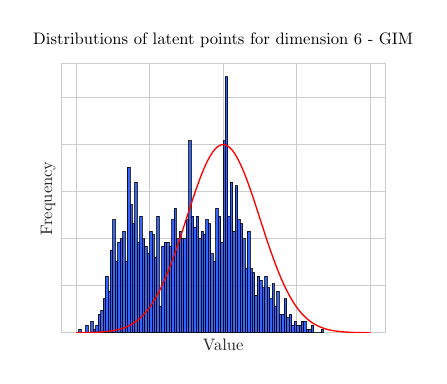
\begin{tikzpicture}[scale=0.6]

\definecolor{blue262255}{RGB}{2,62,255}
\definecolor{darkslategray38}{RGB}{38,38,38}
\definecolor{lightgray204}{RGB}{204,204,204}

\begin{axis}[
axis line style={lightgray204},
tick align=outside,
title={Distributions of latent points for dimension 6 - GIM},
x grid style={lightgray204},
xlabel=\textcolor{darkslategray38}{Value},
xmajorgrids,
xmajorticks=false,
xmin=-4.4, xmax=4.4,
xtick style={color=darkslategray38},
y grid style={lightgray204},
ylabel=\textcolor{darkslategray38}{Frequency},
ymajorgrids,
ymajorticks=false,
ymin=0, ymax=0.570359533676306,
ytick style={color=darkslategray38}
]
\draw[draw=black,fill=blue262255,opacity=0.8,line width=0.48pt] (axis cs:-3.93177318572998,0) rectangle (axis cs:-3.86522126197815,0.00798823055156016);
\draw[draw=black,fill=blue262255,opacity=0.8,line width=0.48pt] (axis cs:-3.86522102355957,0) rectangle (axis cs:-3.79866909980774,0);
\draw[draw=black,fill=blue262255,opacity=0.8,line width=0.48pt] (axis cs:-3.79866933822632,0) rectangle (axis cs:-3.73211741447449,0);
\draw[draw=black,fill=blue262255,opacity=0.8,line width=0.48pt] (axis cs:-3.73211717605591,0) rectangle (axis cs:-3.66556525230408,0.0159764611031203);
\draw[draw=black,fill=blue262255,opacity=0.8,line width=0.48pt] (axis cs:-3.66556549072266,0) rectangle (axis cs:-3.59901356697083,0);
\draw[draw=black,fill=blue262255,opacity=0.8,line width=0.48pt] (axis cs:-3.59901332855225,0) rectangle (axis cs:-3.53246140480042,0.0239646916546805);
\draw[draw=black,fill=blue262255,opacity=0.8,line width=0.48pt] (axis cs:-3.53246164321899,0) rectangle (axis cs:-3.46590971946716,0.00798823055156016);
\draw[draw=black,fill=blue262255,opacity=0.8,line width=0.48pt] (axis cs:-3.46590948104858,0) rectangle (axis cs:-3.39935731887817,0.0159764038685387);
\draw[draw=black,fill=blue262255,opacity=0.8,line width=0.48pt] (axis cs:-3.39935731887817,0) rectangle (axis cs:-3.33280539512634,0.0399411527578008);
\draw[draw=black,fill=blue262255,opacity=0.8,line width=0.48pt] (axis cs:-3.33280563354492,0) rectangle (axis cs:-3.26625370979309,0.0479293833093609);
\draw[draw=black,fill=blue262255,opacity=0.8,line width=0.48pt] (axis cs:-3.26625347137451,0) rectangle (axis cs:-3.19970154762268,0.0718940749640414);
\draw[draw=black,fill=blue262255,opacity=0.8,line width=0.48pt] (axis cs:-3.19970178604126,0) rectangle (axis cs:-3.13314986228943,0.119823458273402);
\draw[draw=black,fill=blue262255,opacity=0.8,line width=0.48pt] (axis cs:-3.13314962387085,0) rectangle (axis cs:-3.06659770011902,0.0878705360671617);
\draw[draw=black,fill=blue262255,opacity=0.8,line width=0.48pt] (axis cs:-3.0665979385376,0) rectangle (axis cs:-3.00004601478577,0.175741072134323);
\draw[draw=black,fill=blue262255,opacity=0.8,line width=0.48pt] (axis cs:-3.00004577636719,0) rectangle (axis cs:-2.93349385261536,0.239646916546805);
\draw[draw=black,fill=blue262255,opacity=0.8,line width=0.48pt] (axis cs:-2.93349409103394,0) rectangle (axis cs:-2.8669421672821,0.151776380479643);
\draw[draw=black,fill=blue262255,opacity=0.8,line width=0.48pt] (axis cs:-2.86694192886353,0) rectangle (axis cs:-2.80039000511169,0.191717533237444);
\draw[draw=black,fill=blue262255,opacity=0.8,line width=0.48pt] (axis cs:-2.80039024353027,0) rectangle (axis cs:-2.73383831977844,0.199705763789004);
\draw[draw=black,fill=blue262255,opacity=0.8,line width=0.48pt] (axis cs:-2.73383808135986,0) rectangle (axis cs:-2.66728615760803,0.215682224892124);
\draw[draw=black,fill=blue262255,opacity=0.8,line width=0.48pt] (axis cs:-2.66728639602661,0) rectangle (axis cs:-2.60073447227478,0.151776380479643);
\draw[draw=black,fill=blue262255,opacity=0.8,line width=0.48pt] (axis cs:-2.6007342338562,0) rectangle (axis cs:-2.53418231010437,0.351482144268647);
\draw[draw=black,fill=blue262255,opacity=0.8,line width=0.48pt] (axis cs:-2.53418231010437,0) rectangle (axis cs:-2.46763014793396,0.271598865765158);
\draw[draw=black,fill=blue262255,opacity=0.8,line width=0.48pt] (axis cs:-2.46763038635254,0) rectangle (axis cs:-2.40107846260071,0.231658685995245);
\draw[draw=black,fill=blue262255,opacity=0.8,line width=0.48pt] (axis cs:-2.40107822418213,0) rectangle (axis cs:-2.3345263004303,0.319529222062406);
\draw[draw=black,fill=blue262255,opacity=0.8,line width=0.48pt] (axis cs:-2.33452653884888,0) rectangle (axis cs:-2.26797461509705,0.191717533237444);
\draw[draw=black,fill=blue262255,opacity=0.8,line width=0.48pt] (axis cs:-2.26797437667847,0) rectangle (axis cs:-2.20142245292664,0.247635147098365);
\draw[draw=black,fill=blue262255,opacity=0.8,line width=0.48pt] (axis cs:-2.20142269134521,0) rectangle (axis cs:-2.13487076759338,0.199705763789004);
\draw[draw=black,fill=blue262255,opacity=0.8,line width=0.48pt] (axis cs:-2.1348705291748,0) rectangle (axis cs:-2.06831860542297,0.183729302685884);
\draw[draw=black,fill=blue262255,opacity=0.8,line width=0.48pt] (axis cs:-2.06831884384155,0) rectangle (axis cs:-2.00176692008972,0.167752841582763);
\draw[draw=black,fill=blue262255,opacity=0.8,line width=0.48pt] (axis cs:-2.00176668167114,0) rectangle (axis cs:-1.93521475791931,0.215682224892124);
\draw[draw=black,fill=blue262255,opacity=0.8,line width=0.48pt] (axis cs:-1.93521475791931,0) rectangle (axis cs:-1.86866283416748,0.207693994340564);
\draw[draw=black,fill=blue262255,opacity=0.8,line width=0.48pt] (axis cs:-1.86866283416748,0) rectangle (axis cs:-1.80211091041565,0.159764611031203);
\draw[draw=black,fill=blue262255,opacity=0.8,line width=0.48pt] (axis cs:-1.80211091041565,0) rectangle (axis cs:-1.73555874824524,0.247634703529563);
\draw[draw=black,fill=blue262255,opacity=0.8,line width=0.48pt] (axis cs:-1.73555886745453,0) rectangle (axis cs:-1.6690069437027,0.0559176138609211);
\draw[draw=black,fill=blue262255,opacity=0.8,line width=0.48pt] (axis cs:-1.6690069437027,0) rectangle (axis cs:-1.60245501995087,0.183729302685884);
\draw[draw=black,fill=blue262255,opacity=0.8,line width=0.48pt] (axis cs:-1.60245501995087,0) rectangle (axis cs:-1.53590309619904,0.191717533237444);
\draw[draw=black,fill=blue262255,opacity=0.8,line width=0.48pt] (axis cs:-1.53590309619904,0) rectangle (axis cs:-1.4693511724472,0.191717533237444);
\draw[draw=black,fill=blue262255,opacity=0.8,line width=0.48pt] (axis cs:-1.4693511724472,0) rectangle (axis cs:-1.40279924869537,0.183729302685884);
\draw[draw=black,fill=blue262255,opacity=0.8,line width=0.48pt] (axis cs:-1.40279924869537,0) rectangle (axis cs:-1.33624732494354,0.239646916546805);
\draw[draw=black,fill=blue262255,opacity=0.8,line width=0.48pt] (axis cs:-1.33624744415283,0) rectangle (axis cs:-1.26969528198242,0.263611136015341);
\draw[draw=black,fill=blue262255,opacity=0.8,line width=0.48pt] (axis cs:-1.26969528198242,0) rectangle (axis cs:-1.20314335823059,0.199705763789004);
\draw[draw=black,fill=blue262255,opacity=0.8,line width=0.48pt] (axis cs:-1.20314335823059,0) rectangle (axis cs:-1.13659143447876,0.215682224892124);
\draw[draw=black,fill=blue262255,opacity=0.8,line width=0.48pt] (axis cs:-1.13659143447876,0) rectangle (axis cs:-1.07003951072693,0.199705763789004);
\draw[draw=black,fill=blue262255,opacity=0.8,line width=0.48pt] (axis cs:-1.07003951072693,0) rectangle (axis cs:-1.0034875869751,0.199705763789004);
\draw[draw=black,fill=blue262255,opacity=0.8,line width=0.48pt] (axis cs:-1.0034875869751,0) rectangle (axis cs:-0.936935663223267,0.239646701916547);
\draw[draw=black,fill=blue262255,opacity=0.8,line width=0.48pt] (axis cs:-0.936935603618622,0) rectangle (axis cs:-0.870383679866791,0.407399758129568);
\draw[draw=black,fill=blue262255,opacity=0.8,line width=0.48pt] (axis cs:-0.870383679866791,0) rectangle (axis cs:-0.80383175611496,0.247635147098365);
\draw[draw=black,fill=blue262255,opacity=0.8,line width=0.48pt] (axis cs:-0.80383175611496,0) rectangle (axis cs:-0.737279832363129,0.223670455443684);
\draw[draw=black,fill=blue262255,opacity=0.8,line width=0.48pt] (axis cs:-0.737279772758484,0) rectangle (axis cs:-0.670727849006653,0.247634925313765);
\draw[draw=black,fill=blue262255,opacity=0.8,line width=0.48pt] (axis cs:-0.670727849006653,0) rectangle (axis cs:-0.604175925254822,0.199705763789004);
\draw[draw=black,fill=blue262255,opacity=0.8,line width=0.48pt] (axis cs:-0.604175925254822,0) rectangle (axis cs:-0.537624001502991,0.215682224892124);
\draw[draw=black,fill=blue262255,opacity=0.8,line width=0.48pt] (axis cs:-0.537624001502991,0) rectangle (axis cs:-0.47107207775116,0.207693901334078);
\draw[draw=black,fill=blue262255,opacity=0.8,line width=0.48pt] (axis cs:-0.471072018146515,0) rectangle (axis cs:-0.404520094394684,0.239646809231628);
\draw[draw=black,fill=blue262255,opacity=0.8,line width=0.48pt] (axis cs:-0.404520094394684,0) rectangle (axis cs:-0.337968170642853,0.231658685995245);
\draw[draw=black,fill=blue262255,opacity=0.8,line width=0.48pt] (axis cs:-0.337968170642853,0) rectangle (axis cs:-0.271416246891022,0.16775276646214);
\draw[draw=black,fill=blue262255,opacity=0.8,line width=0.48pt] (axis cs:-0.271416217088699,0) rectangle (axis cs:-0.204864293336868,0.151776346496496);
\draw[draw=black,fill=blue262255,opacity=0.8,line width=0.48pt] (axis cs:-0.204864263534546,0) rectangle (axis cs:-0.138312339782715,0.263611549178125);
\draw[draw=black,fill=blue262255,opacity=0.8,line width=0.48pt] (axis cs:-0.138312339782715,0) rectangle (axis cs:-0.0717604160308838,0.247635091652178);
\draw[draw=black,fill=blue262255,opacity=0.8,line width=0.48pt] (axis cs:-0.071760393679142,0) rectangle (axis cs:-0.00520846992731094,0.191717490311363);
\draw[draw=black,fill=blue262255,opacity=0.8,line width=0.48pt] (axis cs:-0.0052084531635046,0) rectangle (axis cs:0.0613434687256813,0.407399666911647);
\draw[draw=black,fill=blue262255,opacity=0.8,line width=0.48pt] (axis cs:0.0613434910774231,0) rectangle (axis cs:0.127895414829254,0.543199555882196);
\draw[draw=black,fill=blue262255,opacity=0.8,line width=0.48pt] (axis cs:0.127895414829254,0) rectangle (axis cs:0.194447338581085,0.247635091652178);
\draw[draw=black,fill=blue262255,opacity=0.8,line width=0.48pt] (axis cs:0.194447368383408,0) rectangle (axis cs:0.260999292135239,0.319529150518939);
\draw[draw=black,fill=blue262255,opacity=0.8,line width=0.48pt] (axis cs:0.260999321937561,0) rectangle (axis cs:0.327551245689392,0.215682128308465);
\draw[draw=black,fill=blue262255,opacity=0.8,line width=0.48pt] (axis cs:0.327551245689392,0) rectangle (axis cs:0.394103169441223,0.311540991510846);
\draw[draw=black,fill=blue262255,opacity=0.8,line width=0.48pt] (axis cs:0.394103169441223,0) rectangle (axis cs:0.460655093193054,0.239646809231628);
\draw[draw=black,fill=blue262255,opacity=0.8,line width=0.48pt] (axis cs:0.460655152797699,0) rectangle (axis cs:0.52720707654953,0.23165858225724);
\draw[draw=black,fill=blue262255,opacity=0.8,line width=0.48pt] (axis cs:0.52720707654953,0) rectangle (axis cs:0.593759000301361,0.199705763789004);
\draw[draw=black,fill=blue262255,opacity=0.8,line width=0.48pt] (axis cs:0.593759000301361,0) rectangle (axis cs:0.660310924053192,0.135799919376523);
\draw[draw=black,fill=blue262255,opacity=0.8,line width=0.48pt] (axis cs:0.660310983657837,0) rectangle (axis cs:0.726862907409668,0.215682031724892);
\draw[draw=black,fill=blue262255,opacity=0.8,line width=0.48pt] (axis cs:0.726862907409668,0) rectangle (axis cs:0.793414831161499,0.135799919376523);
\draw[draw=black,fill=blue262255,opacity=0.8,line width=0.48pt] (axis cs:0.793414831161499,0) rectangle (axis cs:0.85996675491333,0.127811688824963);
\draw[draw=black,fill=blue262255,opacity=0.8,line width=0.48pt] (axis cs:0.85996675491333,0) rectangle (axis cs:0.926518678665161,0.0798823055156016);
\draw[draw=black,fill=blue262255,opacity=0.8,line width=0.48pt] (axis cs:0.926518678665161,0) rectangle (axis cs:0.993070602416992,0.119823350958274);
\draw[draw=black,fill=blue262255,opacity=0.8,line width=0.48pt] (axis cs:0.993070602416992,0) rectangle (axis cs:1.05962252616882,0.111835327882809);
\draw[draw=black,fill=blue262255,opacity=0.8,line width=0.48pt] (axis cs:1.05962252616882,0) rectangle (axis cs:1.12617468833923,0.0958585949146696);
\draw[draw=black,fill=blue262255,opacity=0.8,line width=0.48pt] (axis cs:1.12617456912994,0) rectangle (axis cs:1.19272649288177,0.119823458273402);
\draw[draw=black,fill=blue262255,opacity=0.8,line width=0.48pt] (axis cs:1.19272649288177,0) rectangle (axis cs:1.25927841663361,0.0958587666187219);
\draw[draw=black,fill=blue262255,opacity=0.8,line width=0.48pt] (axis cs:1.25927841663361,0) rectangle (axis cs:1.32583034038544,0.0718940749640414);
\draw[draw=black,fill=blue262255,opacity=0.8,line width=0.48pt] (axis cs:1.32583034038544,0) rectangle (axis cs:1.39238226413727,0.103846997170282);
\draw[draw=black,fill=blue262255,opacity=0.8,line width=0.48pt] (axis cs:1.39238226413727,0) rectangle (axis cs:1.4589341878891,0.0559176138609211);
\draw[draw=black,fill=blue262255,opacity=0.8,line width=0.48pt] (axis cs:1.4589341878891,0) rectangle (axis cs:1.52548611164093,0.0878705360671617);
\draw[draw=black,fill=blue262255,opacity=0.8,line width=0.48pt] (axis cs:1.52548599243164,0) rectangle (axis cs:1.59203815460205,0.0399410812144457);
\draw[draw=black,fill=blue262255,opacity=0.8,line width=0.48pt] (axis cs:1.59203815460205,0) rectangle (axis cs:1.65859007835388,0.0399411527578008);
\draw[draw=black,fill=blue262255,opacity=0.8,line width=0.48pt] (axis cs:1.65859007835388,0) rectangle (axis cs:1.72514200210571,0.0718940749640414);
\draw[draw=black,fill=blue262255,opacity=0.8,line width=0.48pt] (axis cs:1.72514200210571,0) rectangle (axis cs:1.79169392585754,0.0319529222062406);
\draw[draw=black,fill=blue262255,opacity=0.8,line width=0.48pt] (axis cs:1.79169392585754,0) rectangle (axis cs:1.85824584960938,0.0399411527578008);
\draw[draw=black,fill=blue262255,opacity=0.8,line width=0.48pt] (axis cs:1.85824584960938,0) rectangle (axis cs:1.92479777336121,0.0159764611031203);
\draw[draw=black,fill=blue262255,opacity=0.8,line width=0.48pt] (axis cs:1.92479777336121,0) rectangle (axis cs:1.99134969711304,0.0239646916546805);
\draw[draw=black,fill=blue262255,opacity=0.8,line width=0.48pt] (axis cs:1.99134981632233,0) rectangle (axis cs:2.05790185928345,0.0159764611031203);
\draw[draw=black,fill=blue262255,opacity=0.8,line width=0.48pt] (axis cs:2.05790138244629,0) rectangle (axis cs:2.12445330619812,0.0159764611031203);
\draw[draw=black,fill=blue262255,opacity=0.8,line width=0.48pt] (axis cs:2.1244535446167,0) rectangle (axis cs:2.19100546836853,0.0239646916546805);
\draw[draw=black,fill=blue262255,opacity=0.8,line width=0.48pt] (axis cs:2.19100546836853,0) rectangle (axis cs:2.25755763053894,0.0239646058028081);
\draw[draw=black,fill=blue262255,opacity=0.8,line width=0.48pt] (axis cs:2.25755739212036,0) rectangle (axis cs:2.32410931587219,0.00798823055156016);
\draw[draw=black,fill=blue262255,opacity=0.8,line width=0.48pt] (axis cs:2.32410955429077,0) rectangle (axis cs:2.3906614780426,0.00798823055156016);
\draw[draw=black,fill=blue262255,opacity=0.8,line width=0.48pt] (axis cs:2.39066123962402,0) rectangle (axis cs:2.45721316337585,0.0159764611031203);
\draw[draw=black,fill=blue262255,opacity=0.8,line width=0.48pt] (axis cs:2.45721340179443,0) rectangle (axis cs:2.52376532554626,0);
\draw[draw=black,fill=blue262255,opacity=0.8,line width=0.48pt] (axis cs:2.52376508712769,0) rectangle (axis cs:2.59031701087952,0);
\draw[draw=black,fill=blue262255,opacity=0.8,line width=0.48pt] (axis cs:2.5903172492981,0) rectangle (axis cs:2.65686917304993,0);
\draw[draw=black,fill=blue262255,opacity=0.8,line width=0.48pt] (axis cs:2.65686893463135,0) rectangle (axis cs:2.72342085838318,0.00798823055156016);
\addplot [thick, red]
table {%
-4 0.000133830225764885
-3.99199199199199 0.000138182046410498
-3.98398398398398 0.000142666228042307
-3.97597597597598 0.000147286481503254
-3.96796796796797 0.000152046611333821
-3.95995995995996 0.000156950517814782
-3.95195195195195 0.00016200219904485
-3.94394394394394 0.00016720575305353
-3.93593593593594 0.000172565379949496
-3.92792792792793 0.00017808538410479
-3.91991991991992 0.000183770176375138
-3.91191191191191 0.000189624276356684
-3.9039039039039 0.000195652314679408
-3.8958958958959 0.000201859035337517
-3.88788788788789 0.000208249298057069
-3.87987987987988 0.000214828080701088
-3.87187187187187 0.000221600481712426
-3.86386386386386 0.0002285717225946
-3.85585585585586 0.000235747150430845
-3.84784784784785 0.000243132240441603
-3.83983983983984 0.000250732598580649
-3.83183183183183 0.000258553964170059
-3.82382382382382 0.000266602212574213
-3.81581581581582 0.000274883357912987
-3.80780780780781 0.000283403555814325
-3.7997997997998 0.000292169106206322
-3.79179179179179 0.000301186456148957
-3.78378378378378 0.0003104622027056
-3.77577577577578 0.000320003095854415
-3.76776776776777 0.000329816041439723
-3.75975975975976 0.000339908104163431
-3.75175175175175 0.00035028651061658
-3.74374374374374 0.000360958652351047
-3.73573573573574 0.000371932088991451
-3.72772772772773 0.000383214551387261
-3.71971971971972 0.000394813944805093
-3.71171171171171 0.000406738352161197
-3.7037037037037 0.000418996037294058
-3.6956956956957 0.00043159544827708
-3.68768768768769 0.00044454522077123
-3.67967967967968 0.000457854181417586
-3.67167167167167 0.000471531351269624
-3.66366366366366 0.000485585949265103
-3.65565565565566 0.000500027395737409
-3.64764764764765 0.000514865315966112
-3.63963963963964 0.000530109543766577
-3.63163163163163 0.000545770125118336
-3.62362362362362 0.000561857321831991
-3.61561561561562 0.00057838161525435
-3.60760760760761 0.000595353710011453
-3.5995995995996 0.000612784537789192
-3.59159159159159 0.000630685261151105
-3.58358358358358 0.000649067277392973
-3.57557557557558 0.000667942222433796
-3.56756756756757 0.000687321974742665
-3.55955955955956 0.000707218659301081
-3.55155155155155 0.000727644651600166
-3.54354354354354 0.000748612581672245
-3.53553553553554 0.000770135338156225
-3.52752752752753 0.000792226072396121
-3.51951951951952 0.00081489820257214
-3.51151151151151 0.000838165417863603
-3.5035035035035 0.000862041682643007
-3.4954954954955 0.000886541240700502
-3.48748748748749 0.00091167861949796
-3.47947947947948 0.000937468634451866
-3.47147147147147 0.000963926393244149
-3.46346346346346 0.000991067300160059
-3.45545545545546 0.0010189070604522
-3.44744744744745 0.00104746168472971
-3.43943943943944 0.0010767474933716
-3.43143143143143 0.00110678112096323
-3.42342342342342 0.00113757952075483
-3.41541541541542 0.00116915996914087
-3.40740740740741 0.00120154007015926
-3.3993993993994 0.00123473776000907
-3.39139139139139 0.00126877131158549
-3.38338338338338 0.00130365933903088
-3.37537537537538 0.00133942080230046
-3.36736736736737 0.00137607501174126
-3.35935935935936 0.001413641632683
-3.35135135135135 0.00145214069003938
-3.34334334334334 0.0014915925729182
-3.33533533533534 0.00153201803923895
-3.32732732732733 0.00157343822035606
-3.31931931931932 0.00161587462568624
-3.31131131131131 0.00165934914733831
-3.3033033033033 0.00170388406474362
-3.2952952952953 0.00174950204928538
-3.28728728728729 0.00179622616892505
-3.27927927927928 0.00184407989282385
-3.27127127127127 0.00189308709595757
-3.26326326326326 0.00194327206372255
-3.25525525525526 0.00199465949653091
-3.24724724724725 0.00204727451439301
-3.23923923923924 0.00210114266148476
-3.23123123123123 0.00215628991069791
-3.22322322322322 0.00221274266817093
-3.21521521521522 0.00227052777779815
-3.20720720720721 0.00232967252571501
-3.1991991991992 0.00239020464475689
-3.19119119119119 0.00245215231888918
-3.18318318318318 0.00251554418760605
-3.17517517517518 0.00258040935029545
-3.16716716716717 0.00264677737056774
-3.15915915915916 0.00271467828054534
-3.15115115115115 0.00278414258511061
-3.14314314314314 0.00285520126610952
-3.13513513513514 0.00292788578650791
-3.12712712712713 0.00300222809449793
-3.11911911911912 0.00307826062755151
-3.11111111111111 0.00315601631641804
-3.1031031031031 0.00323552858906328
-3.0950950950951 0.00331683137454643
-3.08708708708709 0.00339995910683238
-3.07907907907908 0.00348494672853595
-3.07107107107107 0.00357182969459489
-3.06306306306306 0.00366064397586864
-3.05505505505506 0.00375142606265932
-3.04704704704705 0.00384421296815189
-3.03903903903904 0.00393904223176991
-3.03103103103103 0.00403595192244368
-3.02302302302302 0.0041349806417872
-3.01501501501502 0.00423616752718052
-3.00700700700701 0.00433955225475399
-2.998998998999 0.00444517504227068
-2.99099099099099 0.00455307665190355
-2.98298298298298 0.00466329839290368
-2.97497497497497 0.00477588212415564
-2.96696696696697 0.00489087025661667
-2.95895895895896 0.00500830575563558
-2.95095095095095 0.00512823214314763
-2.94294294294294 0.00525069349974172
-2.93493493493493 0.00537573446659573
-2.92692692692693 0.00550340024727644
-2.91891891891892 0.00563373660939975
-2.91091091091091 0.0057667898861475
-2.9029029029029 0.00590260697763674
-2.89489489489489 0.00604123535213746
-2.88688688688689 0.00618272304713484
-2.87887887887888 0.00632711867023164
-2.87087087087087 0.00647447139988703
-2.86286286286286 0.00662483098598741
-2.85485485485485 0.0067782477502453
-2.84684684684685 0.0069347725864219
-2.83883883883884 0.00709445696036946
-2.83083083083083 0.00725735290988893
-2.82282282282282 0.00742351304439893
-2.81481481481481 0.00759299054441176
-2.80680680680681 0.0077658391608121
-2.7987987987988 0.00794211321393437
-2.79079079079079 0.00812186759243432
-2.78278278278278 0.00830515775195071
-2.77477477477477 0.00849203971355293
-2.76676676676677 0.00868257006197001
-2.75875875875876 0.00887680594359712
-2.75075075075075 0.00907480506427511
-2.74274274274274 0.00927662568683898
-2.73473473473473 0.00948232662843099
-2.72672672672673 0.00969196725757422
-2.71871871871872 0.00990560749100246
-2.71071071071071 0.0101233077902421
-2.7027027027027 0.0103451291579421
-2.69469469469469 0.0105711331339476
-2.68668668668669 0.0108013817911136
-2.67867867867868 0.011035937730854
-2.67067067067067 0.0112748640784219
-2.66266266266266 0.0115182244779185
-2.65465465465465 0.0117660830870247
-2.64664664664665 0.0120185045714526
-2.63863863863864 0.0122755540991133
-2.63063063063063 0.0125372973339956
-2.62262262262262 0.0128038004297541
-2.61461461461461 0.0130751300230007
-2.60660660660661 0.0133513532262973
-2.5985985985986 0.0136325376208454
-2.59059059059059 0.0139187512488692
-2.58258258258258 0.014210062605689
-2.57457457457457 0.0145065406314803
-2.56656656656657 0.0148082547027168
-2.55855855855856 0.0151152746232934
-2.55055055055055 0.0154276706153247
-2.54254254254254 0.0157455133096184
-2.53453453453453 0.0160688737358178
-2.52652652652653 0.016397823312213
-2.51851851851852 0.0167324338352151
-2.51051051051051 0.0170727774684938
-2.5025025025025 0.0174189267317727
-2.49449449449449 0.0177709544892815
-2.48648648648649 0.0181289339378627
-2.47847847847848 0.0184929385947284
-2.47047047047047 0.0188630422848682
-2.46246246246246 0.0192393191281025
-2.45445445445445 0.0196218435257817
-2.44644644644645 0.0200106901471285
-2.43843843843844 0.020405933915221
-2.43043043043043 0.0208076499926159
-2.42242242242242 0.0212159137666093
-2.41441441441441 0.0216308008341344
-2.40640640640641 0.0220523869862944
-2.3983983983984 0.0224807481925294
-2.39039039039039 0.022915960584417
-2.38238238238238 0.0233581004391047
-2.37437437437437 0.023807244162374
-2.36636636636637 0.0242634682713357
-2.35835835835836 0.0247268493767558
-2.35035035035035 0.0251974641650118
-2.34234234234234 0.0256753893796796
-2.33433433433433 0.0261607018027501
-2.32632632632633 0.0266534782354775
-2.31831831831832 0.0271537954788581
-2.31031031031031 0.0276617303137407
-2.3023023023023 0.0281773594805703
-2.29429429429429 0.0287007596587648
-2.28628628628629 0.0292320074457259
-2.27827827827828 0.029771179335487
-2.27027027027027 0.0303183516969979
-2.26226226226226 0.0308736007520491
-2.25425425425425 0.0314370025528369
-2.24624624624625 0.0320086329591723
-2.23823823823824 0.0325885676153351
-2.23023023023023 0.0331768819265761
-2.22222222222222 0.0337736510352706
-2.21421421421421 0.0343789497967251
-2.20620620620621 0.0349928527546413
-2.1981981981982 0.0356154341162401
-2.19019019019019 0.0362467677270497
-2.18218218218218 0.0368869270453615
-2.17417417417417 0.0375359851163567
-2.16616616616617 0.03819401454591
-2.15815815815816 0.0388610874740724
-2.15015015015015 0.03953727554824
-2.14214214214214 0.0402226498960119
-2.13413413413413 0.0409172810977437
-2.12612612612613 0.0416212391588003
-2.11811811811812 0.0423345934815158
-2.11011011011011 0.0430574128368641
-2.1021021021021 0.043789765335848
-2.09409409409409 0.0445317184006117
-2.08608608608609 0.0452833387352837
-2.07807807807808 0.0460446922965577
-2.07007007007007 0.0468158442640166
-2.06206206206206 0.0475968590102091
-2.05405405405405 0.0483878000704834
-2.04604604604605 0.0491887301125894
-2.03803803803804 0.0499997109060533
-2.03003003003003 0.0508208032913361
-2.02202202202202 0.0516520671487823
-2.01401401401401 0.0524935613673682
-2.00600600600601 0.053345343813258
-1.997997997998 0.0542074712981785
-1.98998998998999 0.0550799995476186
-1.98198198198198 0.0559629831688668
-1.97397397397397 0.0568564756188931
-1.96596596596597 0.0577605291720876
-1.95795795795796 0.0586751948878651
-1.94994994994995 0.0596005225781457
-1.94194194194194 0.0605365607747232
-1.93393393393393 0.0614833566965309
-1.92592592592593 0.062440956216817
-1.91791791791792 0.06340940383024
-1.90990990990991 0.0643887426198963
-1.9019019019019 0.0653790142242912
-1.89389389389389 0.0663802588042656
-1.88588588588589 0.0673925150098903
-1.87787787787788 0.0684158199473405
-1.86986986986987 0.0694502091457625
-1.86186186186186 0.0704957165241465
-1.85385385385385 0.0715523743582165
-1.84584584584585 0.0726202132473521
-1.83783783783784 0.0736992620815557
-1.82982982982983 0.0747895480084762
-1.82182182182182 0.0758910964005057
-1.81381381381381 0.0770039308219614
-1.80580580580581 0.0781280729963669
-1.7977977977978 0.0792635427738473
-1.78978978978979 0.0804103580986525
-1.78178178178178 0.0815685349768227
-1.77377377377377 0.0827380874440109
-1.76576576576577 0.0839190275334777
-1.75775775775776 0.0851113652442723
-1.74974974974975 0.086315108509615
-1.74174174174174 0.0875302631654975
-1.73373373373373 0.0887568329195139
-1.72572572572573 0.0899948193199405
-1.71771771771772 0.0912442217250772
-1.70970970970971 0.0925050372728685
-1.7017017017017 0.0937772608508177
-1.69369369369369 0.0950608850662112
-1.68568568568569 0.0963559002166691
-1.67767767767768 0.0976622942610365
-1.66966966966967 0.0989800527906321
-1.66166166166166 0.100309159000872
-1.65365365365365 0.10164959366328
-1.64564564564565 0.103001335097907
-1.63763763763764 0.10436435914617
-1.62962962962963 0.105738639144131
-1.62162162162162 0.107124145896225
-1.61361361361361 0.108520847649465
-1.60560560560561 0.10992871006813
-1.5975975975976 0.111347696208955
-1.58958958958959 0.112777766496842
-1.58158158158158 0.114218878701105
-1.57357357357357 0.115670987912262
-1.56556556556557 0.117134046519405
-1.55755755755756 0.11860800418814
-1.54954954954955 0.120092807839133
-1.54154154154154 0.121588401627275
-1.53353353353353 0.123094726921466
-1.52552552552553 0.124611722285057
-1.51751751751752 0.12613932345695
-1.50950950950951 0.127677463333369
-1.5015015015015 0.129226071950339
-1.49349349349349 0.130785076466857
-1.48548548548549 0.132354401148798
-1.47747747747748 0.133933967353555
-1.46946946946947 0.13552369351543
-1.46146146146146 0.137123495131801
-1.45345345345345 0.13873328475006
-1.44544544544545 0.140352971955359
-1.43743743743744 0.141982463359159
-1.42942942942943 0.143621662588612
-1.42142142142142 0.14527047027677
-1.41341341341341 0.146928784053658
-1.40540540540541 0.148596498538208
-1.3973973973974 0.150273505331067
-1.38938938938939 0.151959693008306
-1.38138138138138 0.153654947116025
-1.37337337337337 0.155359150165875
-1.36536536536537 0.157072181631514
-1.35735735735736 0.158793917945997
-1.34934934934935 0.160524232500121
-1.34134134134134 0.16226299564173
-1.33333333333333 0.164010074675994
-1.32532532532533 0.165765333866673
-1.31731731731732 0.167528634438376
-1.30930930930931 0.169299834579821
-1.3013013013013 0.17107878944811
-1.29329329329329 0.172865351174024
-1.28528528528529 0.174659368868355
-1.27727727727728 0.176460688629273
-1.26926926926927 0.178269153550739
-1.26126126126126 0.180084603731981
-1.25325325325325 0.181906876288021
-1.24524524524525 0.183735805361283
-1.23723723723724 0.185571222134271
-1.22922922922923 0.187412954843324
-1.22122122122122 0.18926082879347
-1.21321321321321 0.191114666374361
-1.20520520520521 0.192974287077311
-1.1971971971972 0.194839507513435
-1.18918918918919 0.19671014143289
-1.18118118118118 0.198585999745227
-1.17317317317317 0.200466890540856
-1.16516516516517 0.202352619113618
-1.15715715715716 0.204242987984477
-1.14914914914915 0.206137796926331
-1.14114114114114 0.208036842989938
-1.13313313313313 0.209939920530956
-1.12512512512513 0.21184682123811
-1.11711711711712 0.21375733416247
-1.10910910910911 0.215671245747847
-1.1011011011011 0.217588339862305
-1.09309309309309 0.219508397830784
-1.08508508508509 0.221431198468836
-1.07707707707708 0.223356518117463
-1.06906906906907 0.225284130679063
-1.06106106106106 0.22721380765447
-1.05305305305305 0.229145318181096
-1.04504504504505 0.231078429072154
-1.03703703703704 0.233012904856966
-1.02902902902903 0.234948507822352
-1.02102102102102 0.236884998055083
-1.01301301301301 0.238822133485401
-1.00500500500501 0.24075966993159
-0.996996996996997 0.242697361145593
-0.988988988988989 0.244634958859672
-0.980980980980981 0.246572212834085
-0.972972972972973 0.248508870905785
-0.964964964964965 0.250444679038131
-0.956956956956957 0.252379381371581
-0.948948948948949 0.254312720275385
-0.940940940940941 0.256244436400228
-0.932932932932933 0.258174268731856
-0.924924924924925 0.260101954645624
-0.916916916916917 0.262027229961987
-0.908908908908909 0.263949829002911
-0.900900900900901 0.265869484649172
-0.892892892892893 0.267785928398552
-0.884884884884885 0.269698890424904
-0.876876876876877 0.271608099638066
-0.868868868868869 0.273513283744617
-0.860860860860861 0.275414169309444
-0.852852852852853 0.277310481818125
-0.844844844844845 0.279201945740075
-0.836836836836837 0.281088284592474
-0.828828828828829 0.28296922100493
-0.820820820820821 0.284844476784867
-0.812812812812813 0.286713772983616
-0.804804804804805 0.288576829963198
-0.796796796796797 0.290433367463758
-0.788788788788789 0.292283104671645
-0.780780780780781 0.294125760288111
-0.772772772772773 0.295961052598604
-0.764764764764765 0.29778869954263
-0.756756756756757 0.299608418784177
-0.748748748748749 0.301419927782648
-0.740740740740741 0.303222943864308
-0.732732732732733 0.305017184294205
-0.724724724724725 0.306802366348536
-0.716716716716717 0.308578207387456
-0.708708708708709 0.310344424928268
-0.700700700700701 0.312100736719007
-0.692692692692693 0.313846860812361
-0.684684684684685 0.31558251563992
-0.676676676676677 0.317307420086723
-0.668668668668669 0.319021293566066
-0.660660660660661 0.320723856094559
-0.652652652652653 0.322414828367396
-0.644644644644645 0.324093931833804
-0.636636636636636 0.325760888772662
-0.628628628628629 0.327415422368237
-0.620620620620621 0.329057256786028
-0.612612612612613 0.330686117248681
-0.604604604604605 0.33230173011195
-0.596596596596596 0.333903822940662
-0.588588588588589 0.335492124584683
-0.580580580580581 0.337066365254824
-0.572572572572573 0.338626276598684
-0.564564564564565 0.340171591776383
-0.556556556556556 0.341702045536168
-0.548548548548549 0.343217374289848
-0.54054054054054 0.344717316188045
-0.532532532532533 0.346201611195215
-0.524524524524525 0.347670001164422
-0.516516516516516 0.349122229911825
-0.508508508508509 0.350558043290856
-0.5005005005005 0.351977189266054
-0.492492492492492 0.353379417986526
-0.484484484484485 0.354764481859011
-0.476476476476476 0.356132135620502
-0.468468468468469 0.357482136410418
-0.46046046046046 0.358814243842273
-0.452452452452452 0.360128220074839
-0.444444444444445 0.361423829882744
-0.436436436436436 0.362700840726495
-0.428428428428429 0.363959022821904
-0.42042042042042 0.365198149208855
-0.412412412412412 0.366417995819425
-0.404404404404405 0.3676183415453
-0.396396396396396 0.368798968304465
-0.388388388388389 0.369959661107154
-0.38038038038038 0.37110020812101
-0.372372372372372 0.372220400735444
-0.364364364364365 0.373320033625156
-0.356356356356356 0.374398904812801
-0.348348348348348 0.375456815730761
-0.34034034034034 0.376493571282005
-0.332332332332332 0.377508979900006
-0.324324324324325 0.378502853607702
-0.316316316316316 0.379475008075448
-0.308308308308308 0.380425262677969
-0.3003003003003 0.38135344055026
-0.292292292292292 0.382259368642425
-0.284284284284285 0.38314287777343
-0.276276276276276 0.384003802683735
-0.268268268268268 0.3848419820868
-0.26026026026026 0.385657258719425
-0.252252252252252 0.386449479390916
-0.244244244244244 0.387218495031049
-0.236236236236236 0.387964160736805
-0.228228228228228 0.38868633581787
-0.22022022022022 0.389384883840873
-0.212212212212212 0.390059672672329
-0.204204204204204 0.390710574520297
-0.196196196196196 0.391337465974705
-0.188188188188188 0.39194022804635
-0.18018018018018 0.392518746204527
-0.172172172172172 0.393072910413305
-0.164164164164164 0.393602615166401
-0.156156156156156 0.394107759520658
-0.148148148148148 0.394588247128102
-0.14014014014014 0.395043986266573
-0.132132132132132 0.3954748898689
-0.124124124124124 0.395880875550626
-0.116116116116116 0.396261865636259
-0.108108108108108 0.396617787184037
-0.1001001001001 0.396948572009207
-0.0920920920920922 0.397254156705792
-0.084084084084084 0.397534482666846
-0.0760760760760761 0.39778949610319
-0.0680680680680683 0.39801914806061
-0.06006006006006 0.398223394435522
-0.0520520520520522 0.398402195989086
-0.0440440440440439 0.398555518359772
-0.0360360360360361 0.398683332074364
-0.0280280280280278 0.398785612557403
-0.02002002002002 0.398862340139061
-0.0120120120120122 0.398913500061449
-0.00400400400400391 0.398939082483343
0.00400400400400436 0.398939082483343
0.0120120120120122 0.398913500061449
0.02002002002002 0.398862340139061
0.0280280280280278 0.398785612557403
0.0360360360360357 0.398683332074364
0.0440440440440444 0.398555518359772
0.0520520520520522 0.398402195989086
0.06006006006006 0.398223394435522
0.0680680680680679 0.39801914806061
0.0760760760760757 0.39778949610319
0.0840840840840844 0.397534482666846
0.0920920920920922 0.397254156705792
0.1001001001001 0.396948572009207
0.108108108108108 0.396617787184037
0.116116116116116 0.396261865636259
0.124124124124124 0.395880875550626
0.132132132132132 0.3954748898689
0.14014014014014 0.395043986266573
0.148148148148148 0.394588247128102
0.156156156156156 0.394107759520658
0.164164164164164 0.393602615166401
0.172172172172172 0.393072910413305
0.18018018018018 0.392518746204527
0.188188188188188 0.39194022804635
0.196196196196196 0.391337465974705
0.204204204204204 0.390710574520297
0.212212212212212 0.390059672672329
0.22022022022022 0.389384883840873
0.228228228228228 0.388686335817871
0.236236236236236 0.387964160736805
0.244244244244245 0.387218495031049
0.252252252252252 0.386449479390916
0.26026026026026 0.385657258719425
0.268268268268268 0.3848419820868
0.276276276276276 0.384003802683735
0.284284284284285 0.38314287777343
0.292292292292292 0.382259368642425
0.3003003003003 0.38135344055026
0.308308308308308 0.380425262677969
0.316316316316316 0.379475008075448
0.324324324324325 0.378502853607702
0.332332332332332 0.377508979900006
0.34034034034034 0.376493571282005
0.348348348348348 0.375456815730762
0.356356356356356 0.374398904812801
0.364364364364365 0.373320033625156
0.372372372372372 0.372220400735444
0.38038038038038 0.37110020812101
0.388388388388388 0.369959661107154
0.396396396396397 0.368798968304465
0.404404404404405 0.3676183415453
0.412412412412412 0.366417995819425
0.42042042042042 0.365198149208855
0.428428428428428 0.363959022821904
0.436436436436437 0.362700840726495
0.444444444444445 0.361423829882744
0.452452452452452 0.360128220074839
0.46046046046046 0.358814243842273
0.468468468468468 0.357482136410418
0.476476476476477 0.356132135620502
0.484484484484485 0.354764481859011
0.492492492492492 0.353379417986526
0.5005005005005 0.351977189266054
0.508508508508508 0.350558043290856
0.516516516516517 0.349122229911825
0.524524524524525 0.347670001164422
0.532532532532533 0.346201611195215
0.54054054054054 0.344717316188045
0.548548548548548 0.343217374289848
0.556556556556557 0.341702045536168
0.564564564564565 0.340171591776383
0.572572572572573 0.338626276598684
0.58058058058058 0.337066365254824
0.588588588588588 0.335492124584683
0.596596596596597 0.333903822940662
0.604604604604605 0.33230173011195
0.612612612612613 0.330686117248681
0.62062062062062 0.329057256786028
0.628628628628628 0.327415422368237
0.636636636636637 0.325760888772662
0.644644644644645 0.324093931833804
0.652652652652653 0.322414828367396
0.66066066066066 0.32072385609456
0.668668668668668 0.319021293566066
0.676676676676677 0.317307420086723
0.684684684684685 0.31558251563992
0.692692692692693 0.313846860812361
0.7007007007007 0.312100736719007
0.708708708708708 0.310344424928268
0.716716716716717 0.308578207387456
0.724724724724725 0.306802366348536
0.732732732732733 0.305017184294205
0.74074074074074 0.303222943864308
0.748748748748748 0.301419927782648
0.756756756756757 0.299608418784177
0.764764764764765 0.29778869954263
0.772772772772773 0.295961052598604
0.780780780780781 0.294125760288111
0.788788788788788 0.292283104671645
0.796796796796797 0.290433367463758
0.804804804804805 0.288576829963198
0.812812812812813 0.286713772983616
0.820820820820821 0.284844476784867
0.828828828828828 0.282969221004931
0.836836836836837 0.281088284592474
0.844844844844845 0.279201945740075
0.852852852852853 0.277310481818125
0.860860860860861 0.275414169309444
0.868868868868869 0.273513283744617
0.876876876876877 0.271608099638066
0.884884884884885 0.269698890424904
0.892892892892893 0.267785928398552
0.900900900900901 0.265869484649172
0.908908908908909 0.263949829002911
0.916916916916917 0.262027229961987
0.924924924924925 0.260101954645624
0.932932932932933 0.258174268731856
0.940940940940941 0.256244436400228
0.948948948948949 0.254312720275384
0.956956956956957 0.252379381371581
0.964964964964965 0.250444679038131
0.972972972972973 0.248508870905785
0.980980980980981 0.246572212834085
0.988988988988989 0.244634958859672
0.996996996996997 0.242697361145593
1.00500500500501 0.24075966993159
1.01301301301301 0.238822133485401
1.02102102102102 0.236884998055083
1.02902902902903 0.234948507822352
1.03703703703704 0.233012904856966
1.04504504504505 0.231078429072154
1.05305305305305 0.229145318181096
1.06106106106106 0.22721380765447
1.06906906906907 0.225284130679062
1.07707707707708 0.223356518117463
1.08508508508509 0.221431198468836
1.09309309309309 0.219508397830784
1.1011011011011 0.217588339862305
1.10910910910911 0.215671245747847
1.11711711711712 0.21375733416247
1.12512512512513 0.21184682123811
1.13313313313313 0.209939920530956
1.14114114114114 0.208036842989938
1.14914914914915 0.206137796926331
1.15715715715716 0.204242987984477
1.16516516516517 0.202352619113618
1.17317317317317 0.200466890540856
1.18118118118118 0.198585999745228
1.18918918918919 0.19671014143289
1.1971971971972 0.194839507513435
1.20520520520521 0.192974287077311
1.21321321321321 0.191114666374361
1.22122122122122 0.18926082879347
1.22922922922923 0.187412954843324
1.23723723723724 0.185571222134271
1.24524524524525 0.183735805361283
1.25325325325325 0.181906876288021
1.26126126126126 0.180084603731981
1.26926926926927 0.178269153550739
1.27727727727728 0.176460688629273
1.28528528528529 0.174659368868355
1.29329329329329 0.172865351174024
1.3013013013013 0.17107878944811
1.30930930930931 0.169299834579821
1.31731731731732 0.167528634438376
1.32532532532533 0.165765333866673
1.33333333333333 0.164010074675994
1.34134134134134 0.16226299564173
1.34934934934935 0.160524232500121
1.35735735735736 0.158793917945997
1.36536536536537 0.157072181631514
1.37337337337337 0.155359150165875
1.38138138138138 0.153654947116025
1.38938938938939 0.151959693008306
1.3973973973974 0.150273505331067
1.40540540540541 0.148596498538208
1.41341341341341 0.146928784053658
1.42142142142142 0.14527047027677
1.42942942942943 0.143621662588612
1.43743743743744 0.141982463359159
1.44544544544545 0.140352971955359
1.45345345345345 0.13873328475006
1.46146146146146 0.137123495131801
1.46946946946947 0.13552369351543
1.47747747747748 0.133933967353555
1.48548548548549 0.132354401148798
1.49349349349349 0.130785076466857
1.5015015015015 0.129226071950339
1.50950950950951 0.127677463333369
1.51751751751752 0.12613932345695
1.52552552552553 0.124611722285057
1.53353353353353 0.123094726921466
1.54154154154154 0.121588401627275
1.54954954954955 0.120092807839133
1.55755755755756 0.11860800418814
1.56556556556557 0.117134046519405
1.57357357357357 0.115670987912262
1.58158158158158 0.114218878701105
1.58958958958959 0.112777766496842
1.5975975975976 0.111347696208955
1.60560560560561 0.10992871006813
1.61361361361361 0.108520847649465
1.62162162162162 0.107124145896225
1.62962962962963 0.105738639144131
1.63763763763764 0.10436435914617
1.64564564564565 0.103001335097907
1.65365365365365 0.10164959366328
1.66166166166166 0.100309159000872
1.66966966966967 0.0989800527906321
1.67767767767768 0.0976622942610365
1.68568568568569 0.0963559002166692
1.69369369369369 0.0950608850662112
1.7017017017017 0.0937772608508176
1.70970970970971 0.0925050372728685
1.71771771771772 0.0912442217250772
1.72572572572573 0.0899948193199405
1.73373373373373 0.088756832919514
1.74174174174174 0.0875302631654974
1.74974974974975 0.086315108509615
1.75775775775776 0.0851113652442723
1.76576576576577 0.0839190275334778
1.77377377377377 0.082738087444011
1.78178178178178 0.0815685349768226
1.78978978978979 0.0804103580986525
1.7977977977978 0.0792635427738473
1.80580580580581 0.0781280729963669
1.81381381381381 0.0770039308219615
1.82182182182182 0.0758910964005057
1.82982982982983 0.0747895480084762
1.83783783783784 0.0736992620815557
1.84584584584585 0.0726202132473522
1.85385385385385 0.0715523743582165
1.86186186186186 0.0704957165241465
1.86986986986987 0.0694502091457625
1.87787787787788 0.0684158199473405
1.88588588588589 0.0673925150098903
1.89389389389389 0.0663802588042655
1.9019019019019 0.0653790142242912
1.90990990990991 0.0643887426198963
1.91791791791792 0.06340940383024
1.92592592592593 0.0624409562168171
1.93393393393393 0.0614833566965309
1.94194194194194 0.0605365607747232
1.94994994994995 0.0596005225781457
1.95795795795796 0.0586751948878651
1.96596596596597 0.0577605291720876
1.97397397397397 0.056856475618893
1.98198198198198 0.0559629831688668
1.98998998998999 0.0550799995476186
1.997997997998 0.0542074712981785
2.00600600600601 0.0533453438132581
2.01401401401401 0.0524935613673681
2.02202202202202 0.0516520671487823
2.03003003003003 0.0508208032913361
2.03803803803804 0.0499997109060533
2.04604604604605 0.0491887301125894
2.05405405405405 0.0483878000704834
2.06206206206206 0.0475968590102091
2.07007007007007 0.0468158442640166
2.07807807807808 0.0460446922965577
2.08608608608609 0.0452833387352837
2.09409409409409 0.0445317184006117
2.1021021021021 0.043789765335848
2.11011011011011 0.0430574128368641
2.11811811811812 0.0423345934815158
2.12612612612613 0.0416212391588004
2.13413413413413 0.0409172810977437
2.14214214214214 0.0402226498960119
2.15015015015015 0.03953727554824
2.15815815815816 0.0388610874740724
2.16616616616617 0.03819401454591
2.17417417417417 0.0375359851163567
2.18218218218218 0.0368869270453615
2.19019019019019 0.0362467677270497
2.1981981981982 0.0356154341162401
2.20620620620621 0.0349928527546413
2.21421421421421 0.0343789497967251
2.22222222222222 0.0337736510352706
2.23023023023023 0.0331768819265761
2.23823823823824 0.0325885676153351
2.24624624624625 0.0320086329591724
2.25425425425425 0.0314370025528369
2.26226226226226 0.0308736007520491
2.27027027027027 0.0303183516969979
2.27827827827828 0.029771179335487
2.28628628628629 0.0292320074457259
2.29429429429429 0.0287007596587648
2.3023023023023 0.0281773594805703
2.31031031031031 0.0276617303137407
2.31831831831832 0.0271537954788581
2.32632632632633 0.0266534782354776
2.33433433433433 0.0261607018027501
2.34234234234234 0.0256753893796796
2.35035035035035 0.0251974641650118
2.35835835835836 0.0247268493767558
2.36636636636637 0.0242634682713357
2.37437437437437 0.023807244162374
2.38238238238238 0.0233581004391047
2.39039039039039 0.022915960584417
2.3983983983984 0.0224807481925294
2.40640640640641 0.0220523869862944
2.41441441441441 0.0216308008341344
2.42242242242242 0.0212159137666093
2.43043043043043 0.0208076499926159
2.43843843843844 0.020405933915221
2.44644644644645 0.0200106901471285
2.45445445445445 0.0196218435257817
2.46246246246246 0.0192393191281025
2.47047047047047 0.0188630422848682
2.47847847847848 0.0184929385947284
2.48648648648649 0.0181289339378626
2.49449449449449 0.0177709544892815
2.5025025025025 0.0174189267317727
2.51051051051051 0.0170727774684938
2.51851851851852 0.0167324338352152
2.52652652652653 0.016397823312213
2.53453453453453 0.0160688737358178
2.54254254254254 0.0157455133096184
2.55055055055055 0.0154276706153247
2.55855855855856 0.0151152746232934
2.56656656656657 0.0148082547027168
2.57457457457457 0.0145065406314803
2.58258258258258 0.014210062605689
2.59059059059059 0.0139187512488692
2.5985985985986 0.0136325376208454
2.60660660660661 0.0133513532262973
2.61461461461461 0.0130751300230007
2.62262262262262 0.0128038004297541
2.63063063063063 0.0125372973339956
2.63863863863864 0.0122755540991133
2.64664664664665 0.0120185045714526
2.65465465465465 0.0117660830870247
2.66266266266266 0.0115182244779185
2.67067067067067 0.0112748640784219
2.67867867867868 0.011035937730854
2.68668668668669 0.0108013817911136
2.69469469469469 0.0105711331339476
2.7027027027027 0.0103451291579421
2.71071071071071 0.0101233077902421
2.71871871871872 0.00990560749100247
2.72672672672673 0.00969196725757422
2.73473473473473 0.00948232662843099
2.74274274274274 0.00927662568683898
2.75075075075075 0.00907480506427511
2.75875875875876 0.00887680594359712
2.76676676676677 0.00868257006197001
2.77477477477477 0.00849203971355293
2.78278278278278 0.00830515775195071
2.79079079079079 0.00812186759243432
2.7987987987988 0.00794211321393438
2.80680680680681 0.0077658391608121
2.81481481481481 0.00759299054441176
2.82282282282282 0.00742351304439893
2.83083083083083 0.00725735290988893
2.83883883883884 0.00709445696036947
2.84684684684685 0.0069347725864219
2.85485485485485 0.0067782477502453
2.86286286286286 0.00662483098598741
2.87087087087087 0.00647447139988703
2.87887887887888 0.00632711867023165
2.88688688688689 0.00618272304713484
2.89489489489489 0.00604123535213746
2.9029029029029 0.00590260697763674
2.91091091091091 0.0057667898861475
2.91891891891892 0.00563373660939975
2.92692692692693 0.00550340024727644
2.93493493493493 0.00537573446659573
2.94294294294294 0.00525069349974172
2.95095095095095 0.00512823214314764
2.95895895895896 0.00500830575563558
2.96696696696697 0.00489087025661667
2.97497497497497 0.00477588212415564
2.98298298298298 0.00466329839290368
2.99099099099099 0.00455307665190356
2.998998998999 0.00444517504227067
3.00700700700701 0.00433955225475399
3.01501501501502 0.00423616752718052
3.02302302302302 0.0041349806417872
3.03103103103103 0.00403595192244368
3.03903903903904 0.00393904223176991
3.04704704704705 0.00384421296815189
3.05505505505506 0.00375142606265932
3.06306306306306 0.00366064397586864
3.07107107107107 0.00357182969459489
3.07907907907908 0.00348494672853594
3.08708708708709 0.00339995910683238
3.0950950950951 0.00331683137454643
3.1031031031031 0.00323552858906328
3.11111111111111 0.00315601631641805
3.11911911911912 0.00307826062755151
3.12712712712713 0.00300222809449793
3.13513513513514 0.00292788578650791
3.14314314314314 0.00285520126610952
3.15115115115115 0.00278414258511062
3.15915915915916 0.00271467828054533
3.16716716716717 0.00264677737056774
3.17517517517518 0.00258040935029545
3.18318318318318 0.00251554418760605
3.19119119119119 0.00245215231888919
3.1991991991992 0.00239020464475689
3.20720720720721 0.00232967252571501
3.21521521521522 0.00227052777779815
3.22322322322322 0.00221274266817093
3.23123123123123 0.00215628991069792
3.23923923923924 0.00210114266148476
3.24724724724725 0.00204727451439301
3.25525525525526 0.00199465949653091
3.26326326326326 0.00194327206372255
3.27127127127127 0.00189308709595757
3.27927927927928 0.00184407989282385
3.28728728728729 0.00179622616892505
3.2952952952953 0.00174950204928538
3.3033033033033 0.00170388406474362
3.31131131131131 0.00165934914733832
3.31931931931932 0.00161587462568624
3.32732732732733 0.00157343822035606
3.33533533533534 0.00153201803923895
3.34334334334334 0.0014915925729182
3.35135135135135 0.00145214069003938
3.35935935935936 0.001413641632683
3.36736736736737 0.00137607501174126
3.37537537537538 0.00133942080230046
3.38338338338338 0.00130365933903089
3.39139139139139 0.00126877131158549
3.3993993993994 0.00123473776000907
3.40740740740741 0.00120154007015926
3.41541541541542 0.00116915996914087
3.42342342342342 0.00113757952075483
3.43143143143143 0.00110678112096324
3.43943943943944 0.0010767474933716
3.44744744744745 0.00104746168472971
3.45545545545546 0.0010189070604522
3.46346346346346 0.000991067300160061
3.47147147147147 0.000963926393244148
3.47947947947948 0.000937468634451866
3.48748748748749 0.00091167861949796
3.4954954954955 0.000886541240700502
3.5035035035035 0.000862041682643008
3.51151151151151 0.000838165417863601
3.51951951951952 0.00081489820257214
3.52752752752753 0.000792226072396121
3.53553553553554 0.000770135338156225
3.54354354354354 0.000748612581672247
3.55155155155155 0.000727644651600165
3.55955955955956 0.000707218659301081
3.56756756756757 0.000687321974742665
3.57557557557558 0.000667942222433796
3.58358358358358 0.000649067277392974
3.59159159159159 0.000630685261151104
3.5995995995996 0.000612784537789192
3.60760760760761 0.000595353710011453
3.61561561561562 0.00057838161525435
3.62362362362362 0.000561857321831992
3.63163163163163 0.000545770125118335
3.63963963963964 0.000530109543766577
3.64764764764765 0.000514865315966112
3.65565565565566 0.000500027395737409
3.66366366366366 0.000485585949265104
3.67167167167167 0.000471531351269623
3.67967967967968 0.000457854181417586
3.68768768768769 0.00044454522077123
3.6956956956957 0.00043159544827708
3.7037037037037 0.000418996037294059
3.71171171171171 0.000406738352161196
3.71971971971972 0.000394813944805093
3.72772772772773 0.000383214551387261
3.73573573573574 0.000371932088991452
3.74374374374374 0.000360958652351047
3.75175175175175 0.000350286510616579
3.75975975975976 0.000339908104163431
3.76776776776777 0.000329816041439723
3.77577577577578 0.000320003095854415
3.78378378378378 0.0003104622027056
3.79179179179179 0.000301186456148956
3.7997997997998 0.000292169106206322
3.80780780780781 0.000283403555814325
3.81581581581582 0.000274883357912987
3.82382382382382 0.000266602212574214
3.83183183183183 0.000258553964170059
3.83983983983984 0.000250732598580649
3.84784784784785 0.000243132240441603
3.85585585585586 0.000235747150430845
3.86386386386386 0.000228571722594601
3.87187187187187 0.000221600481712426
3.87987987987988 0.000214828080701088
3.88788788788789 0.000208249298057069
3.8958958958959 0.000201859035337517
3.9039039039039 0.000195652314679408
3.91191191191191 0.000189624276356684
3.91991991991992 0.000183770176375138
3.92792792792793 0.00017808538410479
3.93593593593594 0.000172565379949497
3.94394394394394 0.00016720575305353
3.95195195195195 0.00016200219904485
3.95995995995996 0.000156950517814782
3.96796796796797 0.000152046611333821
3.97597597597598 0.000147286481503255
3.98398398398398 0.000142666228042307
3.99199199199199 0.000138182046410498
4 0.000133830225764885
};
\end{axis}

\end{tikzpicture}

%		\end{subfigure}	
%		
%		\caption{distr beta = 0, module 1}
%	\end{figure}
%	
%		
%		
%		
		

		
	
	
	% loss func only shows part of picture -> towards tsne
		Although loss is used as evaluation metric, it only shows part of the picture. The main objective for the representations is to obtain some form of "decoupled/dis-entanged" features that are more easily separable. This evaluation is done by projecting the latent representations to a 2D plane, via t-SNE. Then datapoints are coloured in depending on their the syllable that was pronounced, eg: "gi" or "ga".
		
		
		

		%Graphs t-sne: Beta = 0	
		%	\begin{figure}[h]
		%		\centering
		%		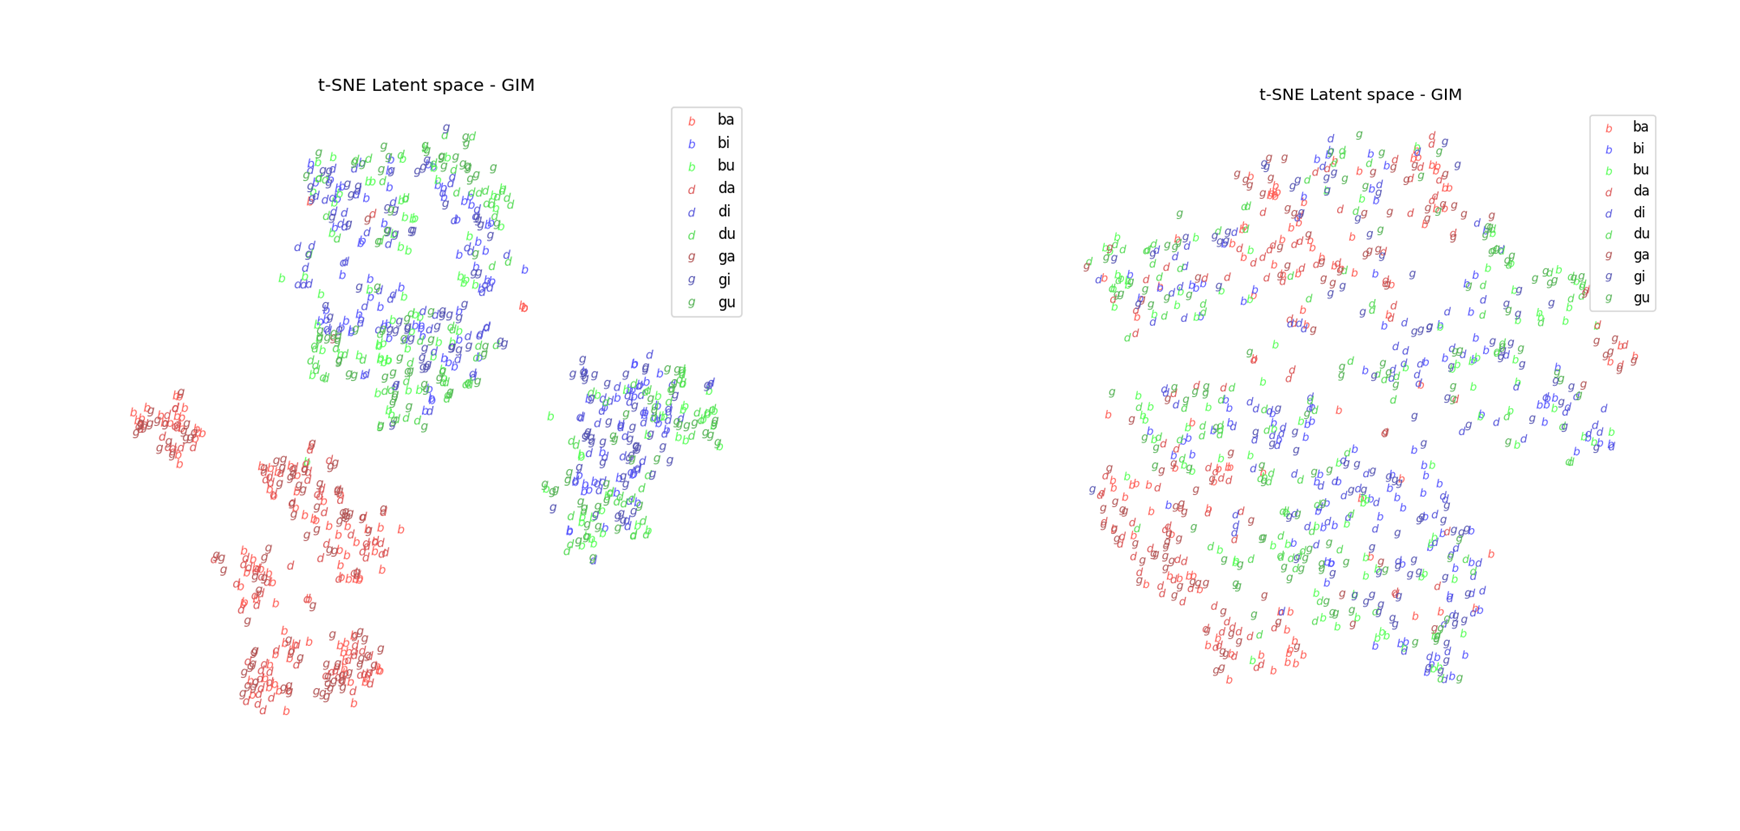
\includegraphics[width=0.7\linewidth]{screenshot023}
		%		\caption{}
		%		\label{fig:tsne_two_module_kld_0}
		%	\end{figure}
		%	
		%	
		%	\begin{figure}[h]
		%		\centering
		%		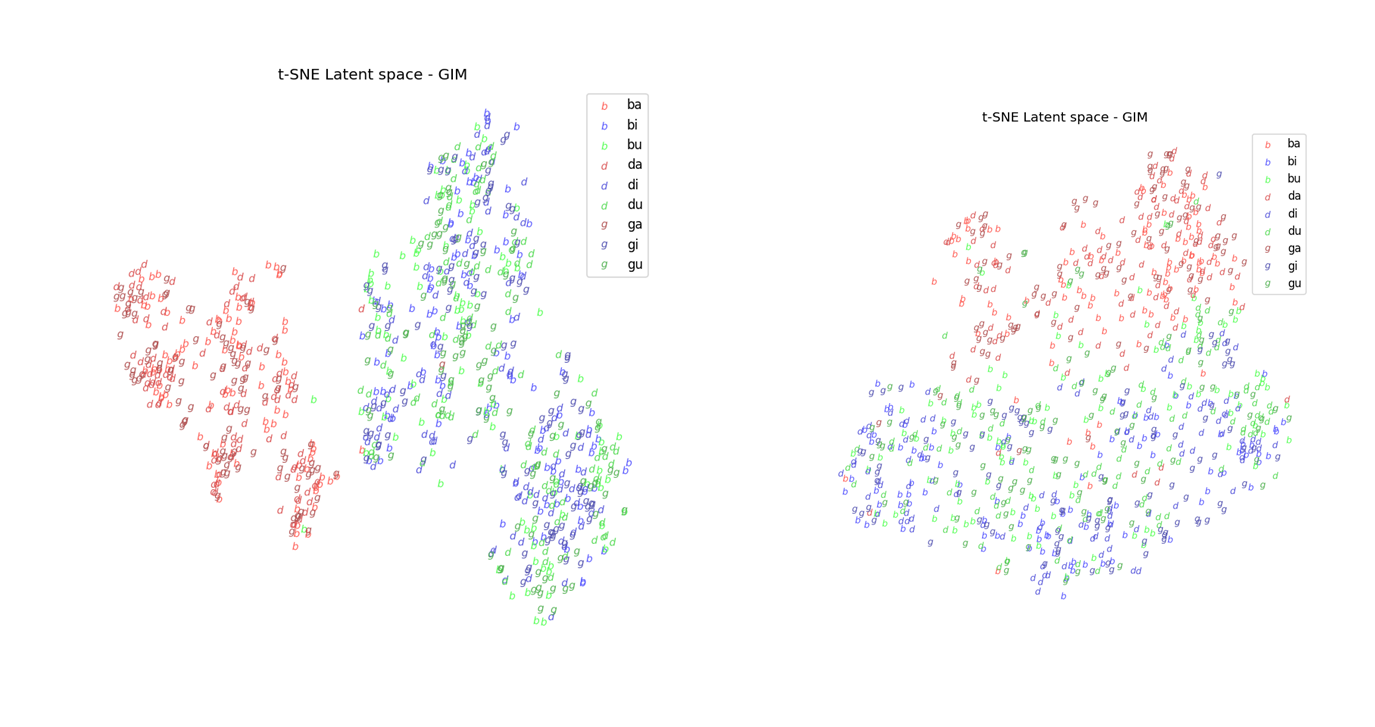
\includegraphics[width=0.7\linewidth]{screenshot024}
		%		\caption{}
		%		\label{fig:tsne_two_module_kld_0033}
		%	\end{figure}
	
	%	
	%	\ref{fig:tsne_two_module_kld_0}: can see that second model harms performance. We believe this can be explained via the learning rate. \ref{fig:tsne_two_module_kld_0033}, there we see that second module performs better separation, indicating that the intermediate KL convergence constraint (causing the normal Gaussian distributions) also serves as a batch normalisation term, and thus resulting in faster convergence.
	%
	%	
	%	---------------------------------------------
	%	
	%	\textbf{T-sne visualisations:}
	%	Multiple models trained, trained GIM, but single module (exact CPC architecture), one with autoregressor and once without autoregressor layer, so only CNN layers. 200 epochs, trained on split up data samples.
	%	
	%	1) Only CNN: We observe better linear separability
	%	\begin{figure}[h]
	%		\centering
	%		\includegraphics[width=0.7\linewidth]{"cpc architecture ONLY CNN t-SNE_latent_space_GIM"}
	%		\caption{}
	%		\label{fig:cpc-architecture-only-cnn-t-snelatentspacegim}
	%	\end{figure}
	%	
	%	2) CNN + 1 autoregressor layer:
	%	\begin{figure}[h]
	%		\centering
	%		\includegraphics[width=0.7\linewidth]{"cpc architecture CNN + GRU t-SNE_latent_space_GIM"}
	%		\caption{}
	%		\label{fig:cpc-architecture-cnn--gru-t-snelatentspacegim}
	%	\end{figure}
	%	
	%	3) This is the pure data visualised (no latent representation).
	%	Were at least doing a bit better than the original data, so that's good! our work is not for nothing.
	%	\begin{figure}[h]
	%		\centering
	%		\includegraphics[width=0.7\linewidth]{"_ t-SNE_latent_space_Original data"}
	%		\caption{}
	%		\label{fig:-t-snelatentspaceoriginal-data}
	%	\end{figure}
	%	
	%	
	%	4) old GIM with all modules each one layer. l1 .. 5 - cnn, l6 = gru. img shows l5 = cnn:
	%	model can more easily distinguish A's from other \textbf{klinkers}. Partly, it kinda makes sense for GIM to learn to separate \textbf{klinkers}. Since they last longer (longer duration), the loss function will more likely randomly sample a subwindow from the "aa's" than from the \textbf{medeklinker} part.
	%	
	
	
	
	
	
	
	
	
	
	
	

%		\begin{figure}
%			\centering
%			\includegraphics[width=0.7\linewidth]{"t-sne kld=0 module 2"}
%			\caption{}
%			\label{fig:t-sne-kld0-module-2}
%		\end{figure}
%		\begin{figure}
%			\centering
%			\includegraphics[width=0.7\linewidth]{"t-sne kld=0.0033 module 1"}
%			\caption{}
%			\label{fig:t-sne-kld0}
%		\end{figure}
%		\begin{figure}
%			\centering
%			\includegraphics[width=0.7\linewidth]{"t-sne kld=0.0033 module 2"}
%			\caption{}
%			\label{fig:t-sne-kld0}
%		\end{figure}
%		\begin{figure}
%			\centering
%			\includegraphics[width=0.7\linewidth]{"t-sne kld=0 module 1"}
%			\caption{}
%			\label{fig:t-sne-kld0-module-1}
%		\end{figure}
	
	
	\subsubsection{T-sne}
	T-distributed stochastic neighbour embedding.
	
	
	Visualising data using T-sne.
	given N high-dimensional objects x1 .. xN. wants to see underlying structure of the data. eg clusters? local structures?
	
	How visiualise very high dimensional data?
	
	Introduction:
		build map where similar data points are moved close to each other and unsimilar points far away. and map in eg 2 or 3 dims. (scatter plot).
		

		
		
		
		
		
		
	

			
			\begin{figure}[ht] % four t-sne images
				\centering
				\begin{subfigure}{0.45\linewidth}
					\centering
					\includegraphics[width=\linewidth]{"t-sne kld=0.0033 module 1"}
					\caption{Module 1: $\beta=0.0035$}
					\label{fig:t-sne-kld33-module1}
				\end{subfigure}
				\hspace{0cm}
				\begin{subfigure}{0.45\linewidth}
					\centering
					\includegraphics[width=\linewidth]{"t-sne kld=0.0033 module 2"}
					\caption{Module 2: $\beta=0.0035$}
					\label{fig:t-sne-kld33-module2}
				\end{subfigure}
				\vspace{0cm}
				\begin{subfigure}{0.45\linewidth}
					\centering					
					\includegraphics[width=\linewidth]{"t-sne kld=0 module 1"}
					\caption{Module 1: $\beta=0$}
					\label{fig:t-sne-kld0-module-1}
				\end{subfigure}
				\hspace{0cm}
				\begin{subfigure}{0.45\linewidth}
					\centering
					\includegraphics[width=\linewidth]{"t-sne kld=0 module 2"}
					\caption{Module 2: $\beta=0.0035$}
					\label{fig:t-sne-kld0-module-2}
				\end{subfigure}
				\caption{My images}
				\label{fig:myimages}
			\end{figure}
		
		
		
	
		
		
		
	
	
	
	


	



\section{Generalisation}
help!!

\begin{figure}[h] % two graphs of subsets
	\centering
	\begin{subfigure}[b]{0.4\textwidth}
		\centering
		% This file was created with tikzplotlib v0.10.1.
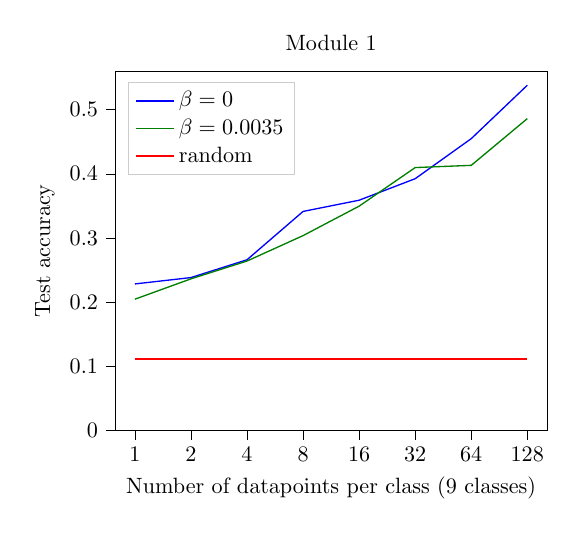
\begin{tikzpicture}[scale=0.8]

\definecolor{darkgray176}{RGB}{176,176,176}
\definecolor{green01270}{RGB}{0,127,0}
\definecolor{lightgray204}{RGB}{204,204,204}

\begin{axis}[
	legend cell align={left},
	legend style={
		fill opacity=0.8,
		draw opacity=1,
		text opacity=1,
		at={(0.03,0.97)},
		anchor=north west,
		draw=lightgray204
	},
	log basis x={2},
	tick align=outside,
	tick pos=left,
	title={Module 1},
	x grid style={darkgray176},
	xlabel={Number of datapoints per class (9 classes)},
	xmin=0.784584097896751, xmax=163.143760296865,
	xmode=log,
	%	%	xtick={0,1,2,3,5,6,7}, % <-- Modify xtick values here
	%		xtick={0,0.30103,0.60206,0.90309,1.50515,1.80618,2.10721}, % <-- Adjusted xtick values
	xticklabels={0, 1,2,4,8,16, 32,64,128}, % <-- Modify xtick labels here
	xtick style={color=black},
	y grid style={darkgray176},
	ylabel={Test accuracy},
	ymin=0.0, ymax=0.559548593309191,
	ytick style={color=black}
	]
\addplot [semithick, blue]
table {%
1 0.228174594470433
2 0.238095226969038
4 0.265873006411961
8 0.341269825526646
16 0.35879628499349
32 0.392361106872559
64 0.454861106872559
128 0.538194427490234
};
\addlegendentry{$\beta = 0$}
\addplot [semithick, green01270]
table {%
1 0.20436507156917
2 0.236111101422991
4 0.263888878141131
8 0.303571417672294
16 0.349537022908529
32 0.409722213745117
64 0.413194427490234
128 0.486111106872559
};
\addlegendentry{$\beta = 0.0035$}
\addplot [semithick, red]
table {%
1 0.111111111111111
2 0.111111111111111
4 0.111111111111111
8 0.111111111111111
16 0.111111111111111
32 0.111111111111111
64 0.111111111111111
128 0.111111111111111
};
\addlegendentry{random}
\end{axis}

\end{tikzpicture}

		%\caption{Caption for the first graph.}
	\end{subfigure}
	\hfill
	\begin{subfigure}[b]{0.4\textwidth}
		\centering
		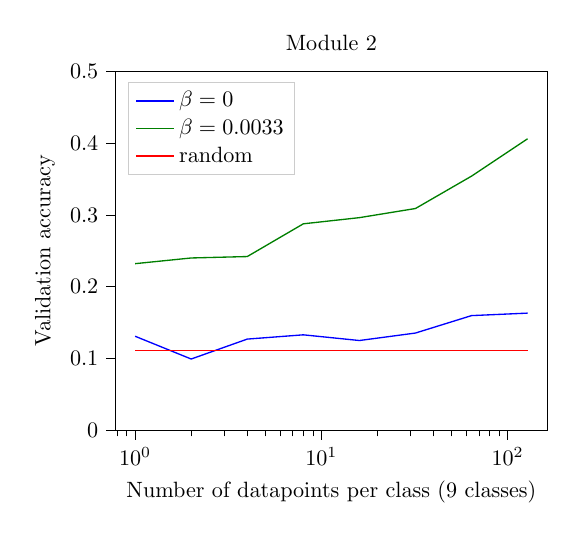
\begin{tikzpicture}[scale=0.8]
				
  \definecolor{darkgray176}{RGB}{176,176,176}
  \definecolor{green01270}{RGB}{0,127,0}
  \definecolor{lightgray204}{RGB}{204,204,204}
  
  \begin{axis}[
    legend cell align={left},
    legend style={
      fill opacity=0.8,
      draw opacity=1,
      text opacity=1,
      at={(0.03,0.97)},
      anchor=north west,
      draw=lightgray204
    },
    log basis x={10},
    tick align=outside,
    tick pos=left,
    title={Module 2},
    x grid style={darkgray176},
    xlabel={Number of datapoints per class (9 classes)},
    xmin=0.784584097896751, xmax=163.143760296865,
    xmode=log,
    xtick style={color=black},
    y grid style={darkgray176},
    ylabel={Validation accuracy},
    ymin=0, ymax=0.5,
    ytick style={color=black}
    ]
    \addplot [semithick, blue]
    table {%
      1 0.130952375956944
      2 0.0992063454219273
      4 0.126984120096479
      8 0.132936503546579
      16 0.124999993642171
      32 0.135416660308838
      64 0.159722213745117
      128 0.163194446563721
    };
    \addlegendentry{$\beta=0$}
    \addplot [semithick, green01270]
    table {%
      1 0.23214284828731
      2 0.240079355239868
      4 0.242063480785915
      8 0.287698405129569
      16 0.296296278635661
      32 0.309027767181396
      64 0.354166641235352
      128 0.40625
    };
    \addlegendentry{$\beta=0.0033$}
    \addplot [semithick, red]
    table {%
      1 0.111111111111111
      2 0.111111111111111
      4 0.111111111111111
      8 0.111111111111111
      16 0.111111111111111
      32 0.111111111111111
      64 0.111111111111111
      128 0.111111111111111
    };
    \addlegendentry{random}
  \end{axis}
  
\end{tikzpicture}
		%\caption{Caption for the second graph.}
	\end{subfigure}
	\caption{Validation accuracy for different subset sizes}
\end{figure}






	


\section{Interpretability}

	\subsection{Decoders for Variational Greedy InfoMax}
		% investigate what info in V-GIM + argue can interpolate
		To investigate what information is contained in V-GIM's representations, we train a decoder on top of each of V-GIM's modules. Contrary to variational autoencoders, V-GIM is fully independent from the decoder and does not require one for training. Furthermore, we analyse the underlying structure the representations obtained from each module. This is achieved by altering representation's component values and observing the effects through the decoder. As we argued in the previous section, this is only possible because V-GIM's encodings is optimised to be approximate to the standard normal. As long as this is case, there are no "gaps" in the latent space around the origin. The decoder will be able to generalise to the altered representations as long as the representations are close to the origin.
		
		We train a decoder for each of V-GIM's modules. As such we can assess the information contained in the final representation, but also the representations of intermediate modules.
		
		% result:
		timesteps in second module captures much wider time frame and first module, so observes different content.
		first module: each component respoble for different frequency.
		
		second module:
		combination of frequencies.
		
		\subsubsection{Decoder architecture}
		We develop two decoders, one for each module. 
		$$
			\text{decoder}^1(\zt^1) = \xt
		$$
		$$
			\text{decoder}^2(\zt^2) = \xt
		$$
		Both decoders' architectures are symmetric to the architecture the V-GIM's encoder. Where the convolutional and max pooling layers are both replaced by transposed convolution layers.
		The architecture for 
		
		\begin{tabular}{|c|c|c|c|}
			\hline
			Layer & Filter size & Stride & Padding \\
			\hline
			TransConv1 & 3 & 1 & 1 \\
			\hline
		\end{tabular}
	
	
	
		% -----
		The decoder consists of a convolutional neural network which takes as input the encodings from V-GIM and is tasked to reconstruct the original data. The decoder is optimised to minimise the mean squared error between mel spectrograms of the original data and the reconstructed data. 
		
		We optimise the decoder with the loss function introduced in [cite] and alter it to use mel spectrograms to better capture the important speech features according to the auditory system. The loss function we use is the following:
		$$
		\mathcal{L}_{\text{decoder}} =\frac{1}{n} \sum_{i=1}^n\left( \log (MEL(y^{(i)})) -\log (MEL(\hat{y} ^{(i)} )) \right)^2
		$$
		
		
	
	
	
	
	% first module:
	
%	class SimpleV2Decoder(GimDecoder):
%	def __init__(self, hidd_channels=32, out_channels=1):
%	super().__init__("Simple_v2_DECODER")
%	
%	# Encoder architecture (Simple v2)
%	kernel_sizes = [10, 8, 3]
%	strides = [4, 3, 1]
%	padding = [2, 2, 1]
%	max_unpool_k_size = 8
%	max_unpool_stride = 4
%	
%	# Decoder architecture
%	self.decoder = nn.Sequential(
%	nn.ConvTranspose1d(hidd_channels, hidd_channels,
%	kernel_sizes[2], stride=strides[2], padding=padding[2]),
%	nn.ReLU(),
%	
%	# Replaces maxpooling
%	nn.ConvTranspose1d(hidd_channels, hidd_channels, max_unpool_k_size,
%	stride=max_unpool_stride, padding=0, output_padding=0),
%	nn.ReLU(),
%	
%	nn.ConvTranspose1d(hidd_channels, hidd_channels,
%	kernel_sizes[1], stride=strides[1], padding=padding[1], output_padding=1),
%	nn.ReLU(),
%	
%	# Replaces maxpooling
%	nn.ConvTranspose1d(hidd_channels, hidd_channels, max_unpool_k_size,
%	stride=max_unpool_stride, padding=0, output_padding=3),
%	nn.ReLU(),
%	
%	nn.ConvTranspose1d(hidd_channels, out_channels,
%	kernel_sizes[0], stride=strides[0], padding=padding[0], output_padding=2),
%	)
%	
%	def forward(self, x):
%	return self.decoder(x)
	
	
	


% Second module:
%
%class SimpleV3DecoderTwoModules(GimDecoder):
%def __init__(self, hidd_channels=32, out_channels=1):
%super().__init__("Simple_v3_2Module_DECODER")
%
%kernel_sizes = [6, 6, 3]
%strides = [2, 2, 1]
%padding = [2, 2, 1]
%
%self.module2 = nn.Sequential(
%nn.ConvTranspose1d(hidd_channels, hidd_channels,
%kernel_sizes[2], stride=strides[2], padding=padding[2]),
%nn.ReLU(),
%nn.ConvTranspose1d(hidd_channels, hidd_channels,
%kernel_sizes[1], stride=strides[1], padding=padding[1], output_padding=0),
%nn.ReLU(),
%nn.ConvTranspose1d(hidd_channels, hidd_channels,
%kernel_sizes[0], stride=strides[0], padding=padding[0], output_padding=0),
%)
%self.module1 = SimpleV2Decoder(hidd_channels, out_channels)
%
%def forward(self, z):
%z = self.module2(z)
%x = self.module1(z)  # SimpleV2Decoder
%return x

	
	
		\subsubsection{Loss function}
		
 % We use five convolutional layers with strides [5, 4, 2, 2, 2], filter-sizes [10, 8, 4, 4, 4] and 512 hidden units with ReLU activations.
	



	
	
	\subsection{Decoder: predictions on test set}
	Fig \ref{fig:bagidi1-model29-true-vs-predicted} displays the reconstructed signal from the vocal sound "ba-gi-di". The two images on the left displays the original signal, while the right two images contain the reconstructed signal.  The upper images displays the signals in time domain, the bottom images spectral domain. The reconstructed signal is an audio sample, for instance which is encoded via Greedy Infomax (up to the fourth (and final) convolution layer), this output is then given to a decoder to reconstruct the original signal.
	
	%TODO: BROKEN 
	%\begin{figure}[h]
	%	\centering
	%	\includegraphics[width=0.7\linewidth]{"../../../../../../../../../GitHub/thesis-fabian-denoodt/GIM/logs/GIM_DECODER_experiment/MSE + scFFT Loss FFT=10240 Lambda=1.0000000/lr_0.0010000/GIM_L4/predictions_model=29/test/bagidi_1, model=29, True vs Predicted"}
	%	\caption{Top left: original, time domain. Bottom left: original }
	%	\label{fig:bagidi1-model29-true-vs-predicted}
	%\end{figure}



